\documentclass[twoside]{book}

% Packages required by doxygen
\usepackage{calc}
\usepackage{doxygen}
\usepackage{graphicx}
\usepackage[utf8]{inputenc}
\usepackage{makeidx}
\usepackage{multicol}
\usepackage{multirow}
\usepackage{textcomp}
\usepackage[table]{xcolor}

% Font selection
\usepackage[T1]{fontenc}
\usepackage{mathptmx}
\usepackage[scaled=.90]{helvet}
\usepackage{courier}
\usepackage{amssymb}
\usepackage{sectsty}
\renewcommand{\familydefault}{\sfdefault}
\allsectionsfont{%
  \fontseries{bc}\selectfont%
  \color{darkgray}%
}
\renewcommand{\DoxyLabelFont}{%
  \fontseries{bc}\selectfont%
  \color{darkgray}%
}

% Page & text layout
\usepackage{geometry}
\geometry{%
  a4paper,%
  top=2.5cm,%
  bottom=2.5cm,%
  left=2.5cm,%
  right=2.5cm%
}
\tolerance=750
\hfuzz=15pt
\hbadness=750
\setlength{\emergencystretch}{15pt}
\setlength{\parindent}{0cm}
\setlength{\parskip}{0.2cm}
\makeatletter
\renewcommand{\paragraph}{%
  \@startsection{paragraph}{4}{0ex}{-1.0ex}{1.0ex}{%
    \normalfont\normalsize\bfseries\SS@parafont%
  }%
}
\renewcommand{\subparagraph}{%
  \@startsection{subparagraph}{5}{0ex}{-1.0ex}{1.0ex}{%
    \normalfont\normalsize\bfseries\SS@subparafont%
  }%
}
\makeatother

% Headers & footers
\usepackage{fancyhdr}
\pagestyle{fancyplain}
\fancyhead[LE]{\fancyplain{}{\bfseries\thepage}}
\fancyhead[CE]{\fancyplain{}{}}
\fancyhead[RE]{\fancyplain{}{\bfseries\leftmark}}
\fancyhead[LO]{\fancyplain{}{\bfseries\rightmark}}
\fancyhead[CO]{\fancyplain{}{}}
\fancyhead[RO]{\fancyplain{}{\bfseries\thepage}}
\fancyfoot[LE]{\fancyplain{}{}}
\fancyfoot[CE]{\fancyplain{}{}}
\fancyfoot[RE]{\fancyplain{}{\bfseries\scriptsize Generated on Tue Dec 15 2015 12\-:22\-:56 for A\-T\-R\-E\-X Python by Doxygen }}
\fancyfoot[LO]{\fancyplain{}{\bfseries\scriptsize Generated on Tue Dec 15 2015 12\-:22\-:56 for A\-T\-R\-E\-X Python by Doxygen }}
\fancyfoot[CO]{\fancyplain{}{}}
\fancyfoot[RO]{\fancyplain{}{}}
\renewcommand{\footrulewidth}{0.4pt}
\renewcommand{\chaptermark}[1]{%
  \markboth{#1}{}%
}
\renewcommand{\sectionmark}[1]{%
  \markright{\thesection\ #1}%
}

% Indices & bibliography
\usepackage{natbib}
\usepackage[titles]{tocloft}
\setcounter{tocdepth}{3}
\setcounter{secnumdepth}{5}
\makeindex

% Hyperlinks (required, but should be loaded last)
\usepackage{ifpdf}
\ifpdf
  \usepackage[pdftex,pagebackref=true]{hyperref}
\else
  \usepackage[ps2pdf,pagebackref=true]{hyperref}
\fi
\hypersetup{%
  colorlinks=true,%
  linkcolor=blue,%
  citecolor=blue,%
  unicode%
}

% Custom commands
\newcommand{\clearemptydoublepage}{%
  \newpage{\pagestyle{empty}\cleardoublepage}%
}


%===== C O N T E N T S =====

\begin{document}

% Titlepage & ToC
\hypersetup{pageanchor=false}
\pagenumbering{roman}
\begin{titlepage}
\vspace*{7cm}
\begin{center}%
{\Large A\-T\-R\-E\-X Python }\\
\vspace*{1cm}
{\large Generated by Doxygen 1.8.5}\\
\vspace*{0.5cm}
{\small Tue Dec 15 2015 12:22:56}\\
\end{center}
\end{titlepage}
\clearemptydoublepage
\tableofcontents
\clearemptydoublepage
\pagenumbering{arabic}
\hypersetup{pageanchor=true}

%--- Begin generated contents ---
\chapter{Namespace Index}
\section{Packages}
Here are the packages with brief descriptions (if available)\-:\begin{DoxyCompactList}
\item\contentsline{section}{\hyperlink{namespace_atrex}{Atrex} }{\pageref{namespace_atrex}}{}
\item\contentsline{section}{\hyperlink{namespaceatrex__utils}{atrex\-\_\-utils} }{\pageref{namespaceatrex__utils}}{}
\item\contentsline{section}{\hyperlink{namespacecongrid}{congrid} }{\pageref{namespacecongrid}}{}
\item\contentsline{section}{\hyperlink{namespacecrystallography}{crystallography} }{\pageref{namespacecrystallography}}{}
\item\contentsline{section}{\hyperlink{namespacegaussfitter}{gaussfitter} }{\pageref{namespacegaussfitter}}{}
\item\contentsline{section}{\hyperlink{namespace_j_c_p_d_s}{J\-C\-P\-D\-S} }{\pageref{namespace_j_c_p_d_s}}{}
\item\contentsline{section}{\hyperlink{namespace_main_peaks}{Main\-Peaks} }{\pageref{namespace_main_peaks}}{}
\item\contentsline{section}{\hyperlink{namespacempfit}{mpfit} }{\pageref{namespacempfit}}{}
\item\contentsline{section}{\hyperlink{namespacemy_detector}{my\-Detector} }{\pageref{namespacemy_detector}}{}
\item\contentsline{section}{\hyperlink{namespacemy_gen_settings_dlg}{my\-Gen\-Settings\-Dlg} }{\pageref{namespacemy_gen_settings_dlg}}{}
\item\contentsline{section}{\hyperlink{namespacemy_image}{my\-Image} }{\pageref{namespacemy_image}}{}
\item\contentsline{section}{\hyperlink{namespacemy_im_display}{my\-Im\-Display} }{\pageref{namespacemy_im_display}}{}
\item\contentsline{section}{\hyperlink{namespacemy_mask}{my\-Mask} }{\pageref{namespacemy_mask}}{}
\item\contentsline{section}{\hyperlink{namespace_my_overlay_dlg}{My\-Overlay\-Dlg} }{\pageref{namespace_my_overlay_dlg}}{}
\item\contentsline{section}{\hyperlink{namespacemy_peak_adjust_dlg}{my\-Peak\-Adjust\-Dlg} }{\pageref{namespacemy_peak_adjust_dlg}}{}
\item\contentsline{section}{\hyperlink{namespacemy_peaks}{my\-Peaks} }{\pageref{namespacemy_peaks}}{}
\item\contentsline{section}{\hyperlink{namespacemy_peak_table}{my\-Peak\-Table} }{\pageref{namespacemy_peak_table}}{}
\item\contentsline{section}{\hyperlink{namespacemy_peak_table_widget}{my\-Peak\-Table\-Widget} }{\pageref{namespacemy_peak_table_widget}}{}
\item\contentsline{section}{\hyperlink{namespace_my_plot_widget}{My\-Plot\-Widget} }{\pageref{namespace_my_plot_widget}}{}
\item\contentsline{section}{\hyperlink{namespacemy_predict}{my\-Predict} }{\pageref{namespacemy_predict}}{}
\item\contentsline{section}{\hyperlink{namespacemy_zm_display}{my\-Zm\-Display} }{\pageref{namespacemy_zm_display}}{}
\item\contentsline{section}{\hyperlink{namespacemy_zm_peak_display}{my\-Zm\-Peak\-Display} }{\pageref{namespacemy_zm_peak_display}}{}
\item\contentsline{section}{\hyperlink{namespacepeak_edit_dlg}{peak\-Edit\-Dlg} }{\pageref{namespacepeak_edit_dlg}}{}
\item\contentsline{section}{\hyperlink{namespacepeak_fit}{peak\-Fit} }{\pageref{namespacepeak_fit}}{}
\item\contentsline{section}{\hyperlink{namespace_peak_object}{Peak\-Object} }{\pageref{namespace_peak_object}}{}
\item\contentsline{section}{\hyperlink{namespace_project}{Project} }{\pageref{namespace_project}}{}
\item\contentsline{section}{\hyperlink{namespace_przemek__testing}{Przemek\-\_\-testing} }{\pageref{namespace_przemek__testing}}{}
\item\contentsline{section}{\hyperlink{namespacesetup}{setup} }{\pageref{namespacesetup}}{}
\item\contentsline{section}{\hyperlink{namespacesimulate_dlg}{simulate\-Dlg} }{\pageref{namespacesimulate_dlg}}{}
\item\contentsline{section}{\hyperlink{namespacetifffile}{tifffile} }{\pageref{namespacetifffile}}{}
\item\contentsline{section}{\hyperlink{namespacevector__math}{vector\-\_\-math} }{\pageref{namespacevector__math}}{}
\end{DoxyCompactList}

\chapter{Hierarchical Index}
\section{Class Hierarchy}
This inheritance list is sorted roughly, but not completely, alphabetically\-:\begin{DoxyCompactList}
\item \contentsline{section}{B\-Y\-T\-E\-\_\-\-S\-T\-R\-I\-N\-G}{\pageref{structBYTE__STRING}}{}
\item dict\begin{DoxyCompactList}
\item \contentsline{section}{tifffile.\-Record}{\pageref{classtifffile_1_1Record}}{}
\begin{DoxyCompactList}
\item \contentsline{section}{tifffile.\-Tiff\-Tags}{\pageref{classtifffile_1_1TiffTags}}{}
\end{DoxyCompactList}
\end{DoxyCompactList}
\item Exception\begin{DoxyCompactList}
\item \contentsline{section}{tifffile.\-Tiff\-Sequence.\-Parse\-Error}{\pageref{classtifffile_1_1TiffSequence_1_1ParseError}}{}
\item \contentsline{section}{tifffile.\-Tiff\-Tag.\-Error}{\pageref{classtifffile_1_1TiffTag_1_1Error}}{}
\end{DoxyCompactList}
\item \contentsline{section}{J\-C\-P\-D\-S.\-J\-C\-P\-D\-S}{\pageref{classJCPDS_1_1JCPDS}}{}
\item \contentsline{section}{mpfit.\-machar}{\pageref{classmpfit_1_1machar}}{}
\item \contentsline{section}{Main\-Peaks.\-Main\-Peaks}{\pageref{classMainPeaks_1_1MainPeaks}}{}
\item \contentsline{section}{mpfit.\-mpfit}{\pageref{classmpfit_1_1mpfit}}{}
\item \contentsline{section}{my\-Image.\-my\-Image}{\pageref{classmyImage_1_1myImage}}{}
\item \contentsline{section}{my\-Peak\-Table.\-my\-Peak}{\pageref{classmyPeakTable_1_1myPeak}}{}
\item \contentsline{section}{my\-Peak\-Table.\-my\-Peak\-Table}{\pageref{classmyPeakTable_1_1myPeakTable}}{}
\item \contentsline{section}{my\-Predict.\-my\-Predict}{\pageref{classmyPredict_1_1myPredict}}{}
\item object\begin{DoxyCompactList}
\item \contentsline{section}{tifffile.\-File\-Handle}{\pageref{classtifffile_1_1FileHandle}}{}
\item \contentsline{section}{tifffile.\-lazyattr}{\pageref{classtifffile_1_1lazyattr}}{}
\item \contentsline{section}{tifffile.\-T\-I\-F\-F\-\_\-\-S\-U\-B\-F\-I\-L\-E\-\_\-\-T\-Y\-P\-E\-S}{\pageref{classtifffile_1_1TIFF__SUBFILE__TYPES}}{}
\item \contentsline{section}{tifffile.\-Tiff\-File}{\pageref{classtifffile_1_1TiffFile}}{}
\item \contentsline{section}{tifffile.\-Tiff\-Page}{\pageref{classtifffile_1_1TiffPage}}{}
\item \contentsline{section}{tifffile.\-Tiff\-Sequence}{\pageref{classtifffile_1_1TiffSequence}}{}
\item \contentsline{section}{tifffile.\-Tiff\-Tag}{\pageref{classtifffile_1_1TiffTag}}{}
\item \contentsline{section}{tifffile.\-Tiff\-Writer}{\pageref{classtifffile_1_1TiffWriter}}{}
\end{DoxyCompactList}
\item \contentsline{section}{peak\-Fit.\-peak\-Fit}{\pageref{classpeakFit_1_1peakFit}}{}
\item \contentsline{section}{Peak\-Object.\-Peak\-Object}{\pageref{classPeakObject_1_1PeakObject}}{}
\item \contentsline{section}{Project.\-Project}{\pageref{classProject_1_1Project}}{}
\item Q\-Dialog\begin{DoxyCompactList}
\item \contentsline{section}{cell\-Path\-Dlg.\-cell\-Path\-Dlg}{\pageref{classcellPathDlg_1_1cellPathDlg}}{}
\item \contentsline{section}{my\-Gen\-Settings\-Dlg.\-my\-Gen\-Settings\-Dlg}{\pageref{classmyGenSettingsDlg_1_1myGenSettingsDlg}}{}
\item \contentsline{section}{My\-Overlay\-Dlg.\-My\-Overlay\-Dlg}{\pageref{classMyOverlayDlg_1_1MyOverlayDlg}}{}
\item \contentsline{section}{my\-Peak\-Adjust\-Dlg.\-my\-Peak\-Adjust\-Dlg}{\pageref{classmyPeakAdjustDlg_1_1myPeakAdjustDlg}}{}
\item \contentsline{section}{peak\-Edit\-Dlg.\-peak\-Edit\-Dlg}{\pageref{classpeakEditDlg_1_1peakEditDlg}}{}
\item \contentsline{section}{simulate\-Dlg.\-simulate\-Dlg}{\pageref{classsimulateDlg_1_1simulateDlg}}{}
\end{DoxyCompactList}
\item Q\-Main\-Window\begin{DoxyCompactList}
\item \contentsline{section}{Atrex.\-Atrex}{\pageref{classAtrex_1_1Atrex}}{}
\end{DoxyCompactList}
\item Q\-Object\begin{DoxyCompactList}
\item \contentsline{section}{my\-Detector.\-my\-Detector}{\pageref{classmyDetector_1_1myDetector}}{}
\item \contentsline{section}{my\-Mask.\-my\-Mask}{\pageref{classmyMask_1_1myMask}}{}
\item \contentsline{section}{my\-Peaks.\-my\-Peaks}{\pageref{classmyPeaks_1_1myPeaks}}{}
\end{DoxyCompactList}
\item Q\-Table\-Widget\begin{DoxyCompactList}
\item \contentsline{section}{my\-Peak\-Table\-Widget.\-my\-Peak\-Table\-Widget}{\pageref{classmyPeakTableWidget_1_1myPeakTableWidget}}{}
\end{DoxyCompactList}
\item Q\-Widget\begin{DoxyCompactList}
\item \contentsline{section}{my\-Im\-Display.\-my\-Im\-Display}{\pageref{classmyImDisplay_1_1myImDisplay}}{}
\item \contentsline{section}{My\-Plot\-Widget.\-My\-Plot\-Widget}{\pageref{classMyPlotWidget_1_1MyPlotWidget}}{}
\item \contentsline{section}{my\-Zm\-Display.\-my\-Zm\-Display}{\pageref{classmyZmDisplay_1_1myZmDisplay}}{}
\item \contentsline{section}{my\-Zm\-Peak\-Display.\-my\-Zm\-Peak\-Display}{\pageref{classmyZmPeakDisplay_1_1myZmPeakDisplay}}{}
\end{DoxyCompactList}
\item \contentsline{section}{J\-C\-P\-D\-S.\-Reflection}{\pageref{classJCPDS_1_1Reflection}}{}
\item \contentsline{section}{Przemek\-\_\-testing.\-tester}{\pageref{classPrzemek__testing_1_1tester}}{}
\end{DoxyCompactList}

\chapter{Class Index}
\section{Class List}
Here are the classes, structs, unions and interfaces with brief descriptions\-:\begin{DoxyCompactList}
\item\contentsline{section}{\hyperlink{class_atrex_1_1_atrex}{Atrex.\-Atrex} \\*\hyperlink{class_atrex_1_1_atrex}{Atrex} Top level class of the \hyperlink{class_atrex_1_1_atrex}{Atrex} software package }{\pageref{class_atrex_1_1_atrex}}{}
\item\contentsline{section}{\hyperlink{struct_b_y_t_e___s_t_r_i_n_g}{B\-Y\-T\-E\-\_\-\-S\-T\-R\-I\-N\-G} }{\pageref{struct_b_y_t_e___s_t_r_i_n_g}}{}
\item\contentsline{section}{\hyperlink{classtifffile_1_1_tiff_tag_1_1_error}{tifffile.\-Tiff\-Tag.\-Error} }{\pageref{classtifffile_1_1_tiff_tag_1_1_error}}{}
\item\contentsline{section}{\hyperlink{classtifffile_1_1_file_handle}{tifffile.\-File\-Handle} }{\pageref{classtifffile_1_1_file_handle}}{}
\item\contentsline{section}{\hyperlink{class_j_c_p_d_s_1_1_j_c_p_d_s}{J\-C\-P\-D\-S.\-J\-C\-P\-D\-S} }{\pageref{class_j_c_p_d_s_1_1_j_c_p_d_s}}{}
\item\contentsline{section}{\hyperlink{classtifffile_1_1lazyattr}{tifffile.\-lazyattr} }{\pageref{classtifffile_1_1lazyattr}}{}
\item\contentsline{section}{\hyperlink{classmpfit_1_1machar}{mpfit.\-machar} }{\pageref{classmpfit_1_1machar}}{}
\item\contentsline{section}{\hyperlink{class_main_peaks_1_1_main_peaks}{Main\-Peaks.\-Main\-Peaks} }{\pageref{class_main_peaks_1_1_main_peaks}}{}
\item\contentsline{section}{\hyperlink{classmpfit_1_1mpfit}{mpfit.\-mpfit} }{\pageref{classmpfit_1_1mpfit}}{}
\item\contentsline{section}{\hyperlink{classmy_detector_1_1my_detector}{my\-Detector.\-my\-Detector} }{\pageref{classmy_detector_1_1my_detector}}{}
\item\contentsline{section}{\hyperlink{classmy_gen_settings_dlg_1_1my_gen_settings_dlg}{my\-Gen\-Settings\-Dlg.\-my\-Gen\-Settings\-Dlg} }{\pageref{classmy_gen_settings_dlg_1_1my_gen_settings_dlg}}{}
\item\contentsline{section}{\hyperlink{classmy_image_1_1my_image}{my\-Image.\-my\-Image} }{\pageref{classmy_image_1_1my_image}}{}
\item\contentsline{section}{\hyperlink{classmy_im_display_1_1my_im_display}{my\-Im\-Display.\-my\-Im\-Display} }{\pageref{classmy_im_display_1_1my_im_display}}{}
\item\contentsline{section}{\hyperlink{classmy_mask_1_1my_mask}{my\-Mask.\-my\-Mask} }{\pageref{classmy_mask_1_1my_mask}}{}
\item\contentsline{section}{\hyperlink{class_my_overlay_dlg_1_1_my_overlay_dlg}{My\-Overlay\-Dlg.\-My\-Overlay\-Dlg} }{\pageref{class_my_overlay_dlg_1_1_my_overlay_dlg}}{}
\item\contentsline{section}{\hyperlink{classmy_peak_table_1_1my_peak}{my\-Peak\-Table.\-my\-Peak} }{\pageref{classmy_peak_table_1_1my_peak}}{}
\item\contentsline{section}{\hyperlink{classmy_peak_adjust_dlg_1_1my_peak_adjust_dlg}{my\-Peak\-Adjust\-Dlg.\-my\-Peak\-Adjust\-Dlg} }{\pageref{classmy_peak_adjust_dlg_1_1my_peak_adjust_dlg}}{}
\item\contentsline{section}{\hyperlink{classmy_peaks_1_1my_peaks}{my\-Peaks.\-my\-Peaks} }{\pageref{classmy_peaks_1_1my_peaks}}{}
\item\contentsline{section}{\hyperlink{classmy_peak_table_1_1my_peak_table}{my\-Peak\-Table.\-my\-Peak\-Table} }{\pageref{classmy_peak_table_1_1my_peak_table}}{}
\item\contentsline{section}{\hyperlink{classmy_peak_table_widget_1_1my_peak_table_widget}{my\-Peak\-Table\-Widget.\-my\-Peak\-Table\-Widget} }{\pageref{classmy_peak_table_widget_1_1my_peak_table_widget}}{}
\item\contentsline{section}{\hyperlink{class_my_plot_widget_1_1_my_plot_widget}{My\-Plot\-Widget.\-My\-Plot\-Widget} }{\pageref{class_my_plot_widget_1_1_my_plot_widget}}{}
\item\contentsline{section}{\hyperlink{classmy_predict_1_1my_predict}{my\-Predict.\-my\-Predict} }{\pageref{classmy_predict_1_1my_predict}}{}
\item\contentsline{section}{\hyperlink{classmy_zm_display_1_1my_zm_display}{my\-Zm\-Display.\-my\-Zm\-Display} }{\pageref{classmy_zm_display_1_1my_zm_display}}{}
\item\contentsline{section}{\hyperlink{classmy_zm_peak_display_1_1my_zm_peak_display}{my\-Zm\-Peak\-Display.\-my\-Zm\-Peak\-Display} }{\pageref{classmy_zm_peak_display_1_1my_zm_peak_display}}{}
\item\contentsline{section}{\hyperlink{classtifffile_1_1_tiff_sequence_1_1_parse_error}{tifffile.\-Tiff\-Sequence.\-Parse\-Error} }{\pageref{classtifffile_1_1_tiff_sequence_1_1_parse_error}}{}
\item\contentsline{section}{\hyperlink{classpeak_edit_dlg_1_1peak_edit_dlg}{peak\-Edit\-Dlg.\-peak\-Edit\-Dlg} }{\pageref{classpeak_edit_dlg_1_1peak_edit_dlg}}{}
\item\contentsline{section}{\hyperlink{classpeak_fit_1_1peak_fit}{peak\-Fit.\-peak\-Fit} }{\pageref{classpeak_fit_1_1peak_fit}}{}
\item\contentsline{section}{\hyperlink{class_peak_object_1_1_peak_object}{Peak\-Object.\-Peak\-Object} }{\pageref{class_peak_object_1_1_peak_object}}{}
\item\contentsline{section}{\hyperlink{class_project_1_1_project}{Project.\-Project} }{\pageref{class_project_1_1_project}}{}
\item\contentsline{section}{\hyperlink{classtifffile_1_1_record}{tifffile.\-Record} }{\pageref{classtifffile_1_1_record}}{}
\item\contentsline{section}{\hyperlink{class_j_c_p_d_s_1_1_reflection}{J\-C\-P\-D\-S.\-Reflection} }{\pageref{class_j_c_p_d_s_1_1_reflection}}{}
\item\contentsline{section}{\hyperlink{classsimulate_dlg_1_1simulate_dlg}{simulate\-Dlg.\-simulate\-Dlg} }{\pageref{classsimulate_dlg_1_1simulate_dlg}}{}
\item\contentsline{section}{\hyperlink{class_przemek__testing_1_1tester}{Przemek\-\_\-testing.\-tester} }{\pageref{class_przemek__testing_1_1tester}}{}
\item\contentsline{section}{\hyperlink{classtifffile_1_1_t_i_f_f___s_u_b_f_i_l_e___t_y_p_e_s}{tifffile.\-T\-I\-F\-F\-\_\-\-S\-U\-B\-F\-I\-L\-E\-\_\-\-T\-Y\-P\-E\-S} }{\pageref{classtifffile_1_1_t_i_f_f___s_u_b_f_i_l_e___t_y_p_e_s}}{}
\item\contentsline{section}{\hyperlink{classtifffile_1_1_tiff_file}{tifffile.\-Tiff\-File} }{\pageref{classtifffile_1_1_tiff_file}}{}
\item\contentsline{section}{\hyperlink{classtifffile_1_1_tiff_page}{tifffile.\-Tiff\-Page} }{\pageref{classtifffile_1_1_tiff_page}}{}
\item\contentsline{section}{\hyperlink{classtifffile_1_1_tiff_sequence}{tifffile.\-Tiff\-Sequence} }{\pageref{classtifffile_1_1_tiff_sequence}}{}
\item\contentsline{section}{\hyperlink{classtifffile_1_1_tiff_tag}{tifffile.\-Tiff\-Tag} }{\pageref{classtifffile_1_1_tiff_tag}}{}
\item\contentsline{section}{\hyperlink{classtifffile_1_1_tiff_tags}{tifffile.\-Tiff\-Tags} }{\pageref{classtifffile_1_1_tiff_tags}}{}
\item\contentsline{section}{\hyperlink{classtifffile_1_1_tiff_writer}{tifffile.\-Tiff\-Writer} }{\pageref{classtifffile_1_1_tiff_writer}}{}
\end{DoxyCompactList}

\chapter{File Index}
\section{File List}
Here is a list of all files with brief descriptions\-:\begin{DoxyCompactList}
\item\contentsline{section}{workdir/atrex/\-Software/\hyperlink{_atrex_8py}{Atrex.\-py} }{\pageref{_atrex_8py}}{}
\item\contentsline{section}{workdir/atrex/\-Software/\hyperlink{atrex__utils_8py}{atrex\-\_\-utils.\-py} }{\pageref{atrex__utils_8py}}{}
\item\contentsline{section}{workdir/atrex/\-Software/\hyperlink{congrid_8py}{congrid.\-py} }{\pageref{congrid_8py}}{}
\item\contentsline{section}{workdir/atrex/\-Software/\hyperlink{crystallography_8py}{crystallography.\-py} }{\pageref{crystallography_8py}}{}
\item\contentsline{section}{workdir/atrex/\-Software/\hyperlink{gaussfitter_8py}{gaussfitter.\-py} }{\pageref{gaussfitter_8py}}{}
\item\contentsline{section}{workdir/atrex/\-Software/\hyperlink{_j_c_p_d_s_8py}{J\-C\-P\-D\-S.\-py} }{\pageref{_j_c_p_d_s_8py}}{}
\item\contentsline{section}{workdir/atrex/\-Software/\hyperlink{_main_peaks_8py}{Main\-Peaks.\-py} }{\pageref{_main_peaks_8py}}{}
\item\contentsline{section}{workdir/atrex/\-Software/\hyperlink{mpfit_8py}{mpfit.\-py} }{\pageref{mpfit_8py}}{}
\item\contentsline{section}{workdir/atrex/\-Software/\hyperlink{my_detector_8py}{my\-Detector.\-py} }{\pageref{my_detector_8py}}{}
\item\contentsline{section}{workdir/atrex/\-Software/\hyperlink{my_gen_settings_dlg_8py}{my\-Gen\-Settings\-Dlg.\-py} }{\pageref{my_gen_settings_dlg_8py}}{}
\item\contentsline{section}{workdir/atrex/\-Software/\hyperlink{my_image_8py}{my\-Image.\-py} }{\pageref{my_image_8py}}{}
\item\contentsline{section}{workdir/atrex/\-Software/\hyperlink{my_im_display_8py}{my\-Im\-Display.\-py} }{\pageref{my_im_display_8py}}{}
\item\contentsline{section}{workdir/atrex/\-Software/\hyperlink{my_mask_8py}{my\-Mask.\-py} }{\pageref{my_mask_8py}}{}
\item\contentsline{section}{workdir/atrex/\-Software/\hyperlink{_my_overlay_dlg_8py}{My\-Overlay\-Dlg.\-py} }{\pageref{_my_overlay_dlg_8py}}{}
\item\contentsline{section}{workdir/atrex/\-Software/\hyperlink{my_peak_adjust_dlg_8py}{my\-Peak\-Adjust\-Dlg.\-py} }{\pageref{my_peak_adjust_dlg_8py}}{}
\item\contentsline{section}{workdir/atrex/\-Software/\hyperlink{my_peaks_8py}{my\-Peaks.\-py} }{\pageref{my_peaks_8py}}{}
\item\contentsline{section}{workdir/atrex/\-Software/\hyperlink{my_peak_table_8py}{my\-Peak\-Table.\-py} }{\pageref{my_peak_table_8py}}{}
\item\contentsline{section}{workdir/atrex/\-Software/\hyperlink{my_peak_table_widget_8py}{my\-Peak\-Table\-Widget.\-py} }{\pageref{my_peak_table_widget_8py}}{}
\item\contentsline{section}{workdir/atrex/\-Software/\hyperlink{_my_plot_widget_8py}{My\-Plot\-Widget.\-py} }{\pageref{_my_plot_widget_8py}}{}
\item\contentsline{section}{workdir/atrex/\-Software/\hyperlink{my_predict_8py}{my\-Predict.\-py} }{\pageref{my_predict_8py}}{}
\item\contentsline{section}{workdir/atrex/\-Software/\hyperlink{my_zm_display_8py}{my\-Zm\-Display.\-py} }{\pageref{my_zm_display_8py}}{}
\item\contentsline{section}{workdir/atrex/\-Software/\hyperlink{my_zm_peak_display_8py}{my\-Zm\-Peak\-Display.\-py} }{\pageref{my_zm_peak_display_8py}}{}
\item\contentsline{section}{workdir/atrex/\-Software/\hyperlink{peak_edit_dlg_8py}{peak\-Edit\-Dlg.\-py} }{\pageref{peak_edit_dlg_8py}}{}
\item\contentsline{section}{workdir/atrex/\-Software/\hyperlink{peak_fit_8py}{peak\-Fit.\-py} }{\pageref{peak_fit_8py}}{}
\item\contentsline{section}{workdir/atrex/\-Software/\hyperlink{_peak_object_8py}{Peak\-Object.\-py} }{\pageref{_peak_object_8py}}{}
\item\contentsline{section}{workdir/atrex/\-Software/\hyperlink{_project_8py}{Project.\-py} }{\pageref{_project_8py}}{}
\item\contentsline{section}{workdir/atrex/\-Software/\hyperlink{_przemek__testing_8py}{Przemek\-\_\-testing.\-py} }{\pageref{_przemek__testing_8py}}{}
\item\contentsline{section}{workdir/atrex/\-Software/\hyperlink{setup_8py}{setup.\-py} }{\pageref{setup_8py}}{}
\item\contentsline{section}{workdir/atrex/\-Software/\hyperlink{simulate_dlg_8py}{simulate\-Dlg.\-py} }{\pageref{simulate_dlg_8py}}{}
\item\contentsline{section}{workdir/atrex/\-Software/\hyperlink{tifffile_8c}{tifffile.\-c} }{\pageref{tifffile_8c}}{}
\item\contentsline{section}{workdir/atrex/\-Software/\hyperlink{tifffile_8py}{tifffile.\-py} }{\pageref{tifffile_8py}}{}
\item\contentsline{section}{workdir/atrex/\-Software/\hyperlink{vector__math_8py}{vector\-\_\-math.\-py} }{\pageref{vector__math_8py}}{}
\end{DoxyCompactList}

\chapter{Namespace Documentation}
\hypertarget{namespace_atrex}{\section{Atrex Namespace Reference}
\label{namespace_atrex}\index{Atrex@{Atrex}}
}
\subsection*{Classes}
\begin{DoxyCompactItemize}
\item 
class \hyperlink{class_atrex_1_1_atrex}{Atrex}
\begin{DoxyCompactList}\small\item\em \hyperlink{class_atrex_1_1_atrex}{Atrex} Top level class of the \hyperlink{class_atrex_1_1_atrex}{Atrex} software package. \end{DoxyCompactList}\end{DoxyCompactItemize}
\subsection*{Variables}
\begin{DoxyCompactItemize}
\item 
tuple \hyperlink{namespace_atrex_afb58c624b98f7c5df49888bb198f1374}{app} = Qt\-Gui.\-Q\-Application(sys.\-argv)
\item 
tuple \hyperlink{namespace_atrex_a1af4daf409e7f1e23d2ff5a8352f4da1}{atrex} = \hyperlink{class_atrex_1_1_atrex}{Atrex}()
\end{DoxyCompactItemize}


\subsection{Variable Documentation}
\hypertarget{namespace_atrex_afb58c624b98f7c5df49888bb198f1374}{\index{Atrex@{Atrex}!app@{app}}
\index{app@{app}!Atrex@{Atrex}}
\subsubsection[{app}]{\setlength{\rightskip}{0pt plus 5cm}tuple Atrex.\-app = Qt\-Gui.\-Q\-Application(sys.\-argv)}}\label{namespace_atrex_afb58c624b98f7c5df49888bb198f1374}
\hypertarget{namespace_atrex_a1af4daf409e7f1e23d2ff5a8352f4da1}{\index{Atrex@{Atrex}!atrex@{atrex}}
\index{atrex@{atrex}!Atrex@{Atrex}}
\subsubsection[{atrex}]{\setlength{\rightskip}{0pt plus 5cm}tuple Atrex.\-atrex = {\bf Atrex}()}}\label{namespace_atrex_a1af4daf409e7f1e23d2ff5a8352f4da1}

\hypertarget{namespaceatrex__utils}{\section{atrex\-\_\-utils Namespace Reference}
\label{namespaceatrex__utils}\index{atrex\-\_\-utils@{atrex\-\_\-utils}}
}
\subsection*{Functions}
\begin{DoxyCompactItemize}
\item 
def \hyperlink{namespaceatrex__utils_a9a9c32b8352e0115e6f6c9ab2b8a1b26}{my\-Square}
\item 
def \hyperlink{namespaceatrex__utils_a7158daee0e5b25be1fe0a18b082cf86d}{get\-Image\-Range}
\end{DoxyCompactItemize}


\subsection{Function Documentation}
\hypertarget{namespaceatrex__utils_a7158daee0e5b25be1fe0a18b082cf86d}{\index{atrex\-\_\-utils@{atrex\-\_\-utils}!get\-Image\-Range@{get\-Image\-Range}}
\index{get\-Image\-Range@{get\-Image\-Range}!atrex_utils@{atrex\-\_\-utils}}
\subsubsection[{get\-Image\-Range}]{\setlength{\rightskip}{0pt plus 5cm}def atrex\-\_\-utils.\-get\-Image\-Range (
\begin{DoxyParamCaption}
\item[{}]{image\-Dir, }
\item[{}]{imstring}
\end{DoxyParamCaption}
)}}\label{namespaceatrex__utils_a7158daee0e5b25be1fe0a18b082cf86d}
\hypertarget{namespaceatrex__utils_a9a9c32b8352e0115e6f6c9ab2b8a1b26}{\index{atrex\-\_\-utils@{atrex\-\_\-utils}!my\-Square@{my\-Square}}
\index{my\-Square@{my\-Square}!atrex_utils@{atrex\-\_\-utils}}
\subsubsection[{my\-Square}]{\setlength{\rightskip}{0pt plus 5cm}def atrex\-\_\-utils.\-my\-Square (
\begin{DoxyParamCaption}
\item[{}]{val}
\end{DoxyParamCaption}
)}}\label{namespaceatrex__utils_a9a9c32b8352e0115e6f6c9ab2b8a1b26}

\hypertarget{namespacecongrid}{\section{congrid Namespace Reference}
\label{namespacecongrid}\index{congrid@{congrid}}
}
\subsection*{Functions}
\begin{DoxyCompactItemize}
\item 
def \hyperlink{namespacecongrid_ad23f482f1eb20fb1171adc7f01716d26}{congrid}
\end{DoxyCompactItemize}


\subsection{Function Documentation}
\hypertarget{namespacecongrid_ad23f482f1eb20fb1171adc7f01716d26}{\index{congrid@{congrid}!congrid@{congrid}}
\index{congrid@{congrid}!congrid@{congrid}}
\subsubsection[{congrid}]{\setlength{\rightskip}{0pt plus 5cm}def congrid.\-congrid (
\begin{DoxyParamCaption}
\item[{}]{a, }
\item[{}]{newdims, }
\item[{}]{method = {\ttfamily 'linear'}, }
\item[{}]{centre = {\ttfamily False}, }
\item[{}]{minusone = {\ttfamily False}}
\end{DoxyParamCaption}
)}}\label{namespacecongrid_ad23f482f1eb20fb1171adc7f01716d26}
\begin{DoxyVerb}Arbitrary resampling of source array to new dimension sizes.
Currently only supports maintaining the same number of dimensions.
To use 1-D arrays, first promote them to shape (x,1).

Uses the same parameters and creates the same co-ordinate lookup points
as IDL''s congrid routine, which apparently originally came from a VAX/VMS
routine of the same name.

method:
neighbour - closest value from original data
nearest and linear - uses n x 1-D interpolations using
                     scipy.interpolate.interp1d
(see Numerical Recipes for validity of use of n 1-D interpolations)
spline - uses ndimage.map_coordinates

centre:
True - interpolation points are at the centres of the bins
False - points are at the front edge of the bin

minusone:
For example- inarray.shape = (i,j) & new dimensions = (x,y)
False - inarray is resampled by factors of (i/x) * (j/y)
True - inarray is resampled by(i-1)/(x-1) * (j-1)/(y-1)
This prevents extrapolation one element beyond bounds of input array.
\end{DoxyVerb}
 
\hypertarget{namespacecrystallography}{\section{crystallography Namespace Reference}
\label{namespacecrystallography}\index{crystallography@{crystallography}}
}
\subsection*{Functions}
\begin{DoxyCompactItemize}
\item 
def \hyperlink{namespacecrystallography_a58171b4824c6f98df0d2200bc258bde2}{A\-\_\-to\-\_\-kev}
\item 
def \hyperlink{namespacecrystallography_a20e6dff641c1326b0062aabcd924cffd}{kev\-\_\-to\-\_\-\-A}
\item 
def \hyperlink{namespacecrystallography_ae86fb13e8f363baa1b13639483c01183}{tth\-\_\-from\-\_\-xyz}
\item 
def \hyperlink{namespacecrystallography_a9efa98c3b1aef1d7beca6fb89086c388}{en\-\_\-from\-\_\-tth\-\_\-and\-\_\-d}
\item 
def \hyperlink{namespacecrystallography_af940a609cdeb81c339448daa1db7c9a9}{en\-\_\-from\-\_\-xyz}
\item 
def \hyperlink{namespacecrystallography_a4df51e2fddc4a9c843028a572a645d8a}{d\-\_\-from\-\_\-tth\-\_\-and\-\_\-en}
\item 
def \hyperlink{namespacecrystallography_aa131e8fb34e0833ceaff1dcdf8337a60}{tth\-\_\-from\-\_\-en\-\_\-and\-\_\-d}
\item 
def \hyperlink{namespacecrystallography_a797dc74ad0fe257371737f35f5bf44d8}{tth\-\_\-from\-\_\-hkl\-\_\-and\-\_\-lp}
\item 
def \hyperlink{namespacecrystallography_a5f7e74ec1d11c8cfb020d7ebb515c0c5}{d\-\_\-from\-\_\-lp\-\_\-and\-\_\-hkl}
\item 
def \hyperlink{namespacecrystallography_a0c041a7a2849ec884fe8bd234b7e04dd}{equivalent}
\item 
def \hyperlink{namespacecrystallography_a1b5cfcfc56bb0c43e2898b18c2ae0f31}{b\-\_\-from\-\_\-lp}
\item 
def \hyperlink{namespacecrystallography_a108a8b1c5312871f58ebcbe980b37801}{dotprod}
\item 
def \hyperlink{namespacecrystallography_aea2c4d89da7b6b57a4d947a51ed67c9e}{vlength}
\item 
def \hyperlink{namespacecrystallography_aae60d18338e58a21bb9abd24beecbe42}{ang}
\item 
def \hyperlink{namespacecrystallography_afa94b4aac1d8fd726f31e98915aa3833}{lp\-\_\-from\-\_\-ub}
\item 
def \hyperlink{namespacecrystallography_a49712413ea299a47440e3db9b0d187cd}{V\-\_\-from\-\_\-lp}
\item 
def \hyperlink{namespacecrystallography_ace21f698f6a91880ff79b26cce3d44a1}{V\-\_\-from\-\_\-ub}
\item 
def \hyperlink{namespacecrystallography_a8b7bd586e750f963562e8811b171dc85}{U\-\_\-from\-\_\-ub}
\item 
def \hyperlink{namespacecrystallography_ade33673c59999578962f7e3574fd66f5}{hkl\-\_\-from\-\_\-ub\-\_\-and\-\_\-xyz}
\item 
def \hyperlink{namespacecrystallography_a1135eb3d895d4db119f03dfe03b16246}{find\-\_\-possible\-\_\-hkls}
\item 
def \hyperlink{namespacecrystallography_afc7e18304cb893ba82f482dda7a8203a}{flags\-\_\-from\-\_\-sym}
\item 
def \hyperlink{namespacecrystallography_a4e57db686b17b444803bf0b345633bcc}{syst\-\_\-extinction}
\item 
def \hyperlink{namespacecrystallography_a3e5709b266157e0701be4d336c074648}{apply\-\_\-symmetry\-\_\-to\-\_\-lp}
\item 
def \hyperlink{namespacecrystallography_aceeb721a52e4341dc482f2830ab13c9c}{angle\-\_\-between\-\_\-hkls}
\item 
def \hyperlink{namespacecrystallography_af905b3d3c9e00d94a3bda5150b55d8bd}{calc\-\_\-ub\-\_\-from\-\_\-three}
\item 
def \hyperlink{namespacecrystallography_a5c3a3554b9a344670d7ea9126758f76d}{get\-\_\-omega}
\begin{DoxyCompactList}\small\item\em get\-\_\-omega -- From xyz and energy calculates the omega angle (in deg) at which xyz will come into diffracting position during omega scan at chi 0 if diffraction position inaccessible in omega scan returns \mbox{[}-\/1000,-\/1000\mbox{]} \end{DoxyCompactList}\item 
def \hyperlink{namespacecrystallography_a135f57254d70c8f690eb769d3ad18437}{general\-\_\-axis}
\item 
def \hyperlink{namespacecrystallography_ada28fca5d9f6fd5ab456edc3e32713e1}{solve\-\_\-general\-\_\-axis}
\item 
def \hyperlink{namespacecrystallography_a0a424f36ab371104637e16161cbf9b73}{sincos}
\item 
def \hyperlink{namespacecrystallography_a0da34711a0fdb2fc186eac5a965e35d6}{open\-\_\-\-U\-B}
\end{DoxyCompactItemize}
\subsection*{Variables}
\begin{DoxyCompactItemize}
\item 
int \hyperlink{namespacecrystallography_ad28d74622030c2011af7636d2657ed99}{D\-T\-O\-R} = math.\-pi/180
\item 
int \hyperlink{namespacecrystallography_ad0848788e86c4a194771f24fb582c3c8}{radeg} = 180
\end{DoxyCompactItemize}


\subsection{Function Documentation}
\hypertarget{namespacecrystallography_a58171b4824c6f98df0d2200bc258bde2}{\index{crystallography@{crystallography}!A\-\_\-to\-\_\-kev@{A\-\_\-to\-\_\-kev}}
\index{A\-\_\-to\-\_\-kev@{A\-\_\-to\-\_\-kev}!crystallography@{crystallography}}
\subsubsection[{A\-\_\-to\-\_\-kev}]{\setlength{\rightskip}{0pt plus 5cm}def crystallography.\-A\-\_\-to\-\_\-kev (
\begin{DoxyParamCaption}
\item[{}]{la}
\end{DoxyParamCaption}
)}}\label{namespacecrystallography_a58171b4824c6f98df0d2200bc258bde2}
\hypertarget{namespacecrystallography_aae60d18338e58a21bb9abd24beecbe42}{\index{crystallography@{crystallography}!ang@{ang}}
\index{ang@{ang}!crystallography@{crystallography}}
\subsubsection[{ang}]{\setlength{\rightskip}{0pt plus 5cm}def crystallography.\-ang (
\begin{DoxyParamCaption}
\item[{}]{v, }
\item[{}]{w}
\end{DoxyParamCaption}
)}}\label{namespacecrystallography_aae60d18338e58a21bb9abd24beecbe42}
\hypertarget{namespacecrystallography_aceeb721a52e4341dc482f2830ab13c9c}{\index{crystallography@{crystallography}!angle\-\_\-between\-\_\-hkls@{angle\-\_\-between\-\_\-hkls}}
\index{angle\-\_\-between\-\_\-hkls@{angle\-\_\-between\-\_\-hkls}!crystallography@{crystallography}}
\subsubsection[{angle\-\_\-between\-\_\-hkls}]{\setlength{\rightskip}{0pt plus 5cm}def crystallography.\-angle\-\_\-between\-\_\-hkls (
\begin{DoxyParamCaption}
\item[{}]{h1, }
\item[{}]{h2, }
\item[{}]{lp}
\end{DoxyParamCaption}
)}}\label{namespacecrystallography_aceeb721a52e4341dc482f2830ab13c9c}
\hypertarget{namespacecrystallography_a3e5709b266157e0701be4d336c074648}{\index{crystallography@{crystallography}!apply\-\_\-symmetry\-\_\-to\-\_\-lp@{apply\-\_\-symmetry\-\_\-to\-\_\-lp}}
\index{apply\-\_\-symmetry\-\_\-to\-\_\-lp@{apply\-\_\-symmetry\-\_\-to\-\_\-lp}!crystallography@{crystallography}}
\subsubsection[{apply\-\_\-symmetry\-\_\-to\-\_\-lp}]{\setlength{\rightskip}{0pt plus 5cm}def crystallography.\-apply\-\_\-symmetry\-\_\-to\-\_\-lp (
\begin{DoxyParamCaption}
\item[{}]{lp, }
\item[{}]{ch, }
\item[{}]{sym}
\end{DoxyParamCaption}
)}}\label{namespacecrystallography_a3e5709b266157e0701be4d336c074648}
\hypertarget{namespacecrystallography_a1b5cfcfc56bb0c43e2898b18c2ae0f31}{\index{crystallography@{crystallography}!b\-\_\-from\-\_\-lp@{b\-\_\-from\-\_\-lp}}
\index{b\-\_\-from\-\_\-lp@{b\-\_\-from\-\_\-lp}!crystallography@{crystallography}}
\subsubsection[{b\-\_\-from\-\_\-lp}]{\setlength{\rightskip}{0pt plus 5cm}def crystallography.\-b\-\_\-from\-\_\-lp (
\begin{DoxyParamCaption}
\item[{}]{lp}
\end{DoxyParamCaption}
)}}\label{namespacecrystallography_a1b5cfcfc56bb0c43e2898b18c2ae0f31}
\hypertarget{namespacecrystallography_af905b3d3c9e00d94a3bda5150b55d8bd}{\index{crystallography@{crystallography}!calc\-\_\-ub\-\_\-from\-\_\-three@{calc\-\_\-ub\-\_\-from\-\_\-three}}
\index{calc\-\_\-ub\-\_\-from\-\_\-three@{calc\-\_\-ub\-\_\-from\-\_\-three}!crystallography@{crystallography}}
\subsubsection[{calc\-\_\-ub\-\_\-from\-\_\-three}]{\setlength{\rightskip}{0pt plus 5cm}def crystallography.\-calc\-\_\-ub\-\_\-from\-\_\-three (
\begin{DoxyParamCaption}
\item[{}]{hkls, }
\item[{}]{xyzs}
\end{DoxyParamCaption}
)}}\label{namespacecrystallography_af905b3d3c9e00d94a3bda5150b55d8bd}
\hypertarget{namespacecrystallography_a5f7e74ec1d11c8cfb020d7ebb515c0c5}{\index{crystallography@{crystallography}!d\-\_\-from\-\_\-lp\-\_\-and\-\_\-hkl@{d\-\_\-from\-\_\-lp\-\_\-and\-\_\-hkl}}
\index{d\-\_\-from\-\_\-lp\-\_\-and\-\_\-hkl@{d\-\_\-from\-\_\-lp\-\_\-and\-\_\-hkl}!crystallography@{crystallography}}
\subsubsection[{d\-\_\-from\-\_\-lp\-\_\-and\-\_\-hkl}]{\setlength{\rightskip}{0pt plus 5cm}def crystallography.\-d\-\_\-from\-\_\-lp\-\_\-and\-\_\-hkl (
\begin{DoxyParamCaption}
\item[{}]{lp, }
\item[{}]{hkl}
\end{DoxyParamCaption}
)}}\label{namespacecrystallography_a5f7e74ec1d11c8cfb020d7ebb515c0c5}
\hypertarget{namespacecrystallography_a4df51e2fddc4a9c843028a572a645d8a}{\index{crystallography@{crystallography}!d\-\_\-from\-\_\-tth\-\_\-and\-\_\-en@{d\-\_\-from\-\_\-tth\-\_\-and\-\_\-en}}
\index{d\-\_\-from\-\_\-tth\-\_\-and\-\_\-en@{d\-\_\-from\-\_\-tth\-\_\-and\-\_\-en}!crystallography@{crystallography}}
\subsubsection[{d\-\_\-from\-\_\-tth\-\_\-and\-\_\-en}]{\setlength{\rightskip}{0pt plus 5cm}def crystallography.\-d\-\_\-from\-\_\-tth\-\_\-and\-\_\-en (
\begin{DoxyParamCaption}
\item[{}]{atth, }
\item[{}]{en}
\end{DoxyParamCaption}
)}}\label{namespacecrystallography_a4df51e2fddc4a9c843028a572a645d8a}
\hypertarget{namespacecrystallography_a108a8b1c5312871f58ebcbe980b37801}{\index{crystallography@{crystallography}!dotprod@{dotprod}}
\index{dotprod@{dotprod}!crystallography@{crystallography}}
\subsubsection[{dotprod}]{\setlength{\rightskip}{0pt plus 5cm}def crystallography.\-dotprod (
\begin{DoxyParamCaption}
\item[{}]{v, }
\item[{}]{w}
\end{DoxyParamCaption}
)}}\label{namespacecrystallography_a108a8b1c5312871f58ebcbe980b37801}
\hypertarget{namespacecrystallography_a9efa98c3b1aef1d7beca6fb89086c388}{\index{crystallography@{crystallography}!en\-\_\-from\-\_\-tth\-\_\-and\-\_\-d@{en\-\_\-from\-\_\-tth\-\_\-and\-\_\-d}}
\index{en\-\_\-from\-\_\-tth\-\_\-and\-\_\-d@{en\-\_\-from\-\_\-tth\-\_\-and\-\_\-d}!crystallography@{crystallography}}
\subsubsection[{en\-\_\-from\-\_\-tth\-\_\-and\-\_\-d}]{\setlength{\rightskip}{0pt plus 5cm}def crystallography.\-en\-\_\-from\-\_\-tth\-\_\-and\-\_\-d (
\begin{DoxyParamCaption}
\item[{}]{atth, }
\item[{}]{d}
\end{DoxyParamCaption}
)}}\label{namespacecrystallography_a9efa98c3b1aef1d7beca6fb89086c388}
\hypertarget{namespacecrystallography_af940a609cdeb81c339448daa1db7c9a9}{\index{crystallography@{crystallography}!en\-\_\-from\-\_\-xyz@{en\-\_\-from\-\_\-xyz}}
\index{en\-\_\-from\-\_\-xyz@{en\-\_\-from\-\_\-xyz}!crystallography@{crystallography}}
\subsubsection[{en\-\_\-from\-\_\-xyz}]{\setlength{\rightskip}{0pt plus 5cm}def crystallography.\-en\-\_\-from\-\_\-xyz (
\begin{DoxyParamCaption}
\item[{}]{xyz}
\end{DoxyParamCaption}
)}}\label{namespacecrystallography_af940a609cdeb81c339448daa1db7c9a9}
\hypertarget{namespacecrystallography_a0c041a7a2849ec884fe8bd234b7e04dd}{\index{crystallography@{crystallography}!equivalent@{equivalent}}
\index{equivalent@{equivalent}!crystallography@{crystallography}}
\subsubsection[{equivalent}]{\setlength{\rightskip}{0pt plus 5cm}def crystallography.\-equivalent (
\begin{DoxyParamCaption}
\item[{}]{hkl1, }
\item[{}]{hkl2, }
\item[{}]{exti}
\end{DoxyParamCaption}
)}}\label{namespacecrystallography_a0c041a7a2849ec884fe8bd234b7e04dd}
\hypertarget{namespacecrystallography_a1135eb3d895d4db119f03dfe03b16246}{\index{crystallography@{crystallography}!find\-\_\-possible\-\_\-hkls@{find\-\_\-possible\-\_\-hkls}}
\index{find\-\_\-possible\-\_\-hkls@{find\-\_\-possible\-\_\-hkls}!crystallography@{crystallography}}
\subsubsection[{find\-\_\-possible\-\_\-hkls}]{\setlength{\rightskip}{0pt plus 5cm}def crystallography.\-find\-\_\-possible\-\_\-hkls (
\begin{DoxyParamCaption}
\item[{}]{d1, }
\item[{}]{lp, }
\item[{}]{dtol, }
\item[{}]{hkl}
\end{DoxyParamCaption}
)}}\label{namespacecrystallography_a1135eb3d895d4db119f03dfe03b16246}
\hypertarget{namespacecrystallography_afc7e18304cb893ba82f482dda7a8203a}{\index{crystallography@{crystallography}!flags\-\_\-from\-\_\-sym@{flags\-\_\-from\-\_\-sym}}
\index{flags\-\_\-from\-\_\-sym@{flags\-\_\-from\-\_\-sym}!crystallography@{crystallography}}
\subsubsection[{flags\-\_\-from\-\_\-sym}]{\setlength{\rightskip}{0pt plus 5cm}def crystallography.\-flags\-\_\-from\-\_\-sym (
\begin{DoxyParamCaption}
\item[{}]{sym}
\end{DoxyParamCaption}
)}}\label{namespacecrystallography_afc7e18304cb893ba82f482dda7a8203a}
\hypertarget{namespacecrystallography_a135f57254d70c8f690eb769d3ad18437}{\index{crystallography@{crystallography}!general\-\_\-axis@{general\-\_\-axis}}
\index{general\-\_\-axis@{general\-\_\-axis}!crystallography@{crystallography}}
\subsubsection[{general\-\_\-axis}]{\setlength{\rightskip}{0pt plus 5cm}def crystallography.\-general\-\_\-axis (
\begin{DoxyParamCaption}
\item[{}]{A, }
\item[{}]{vec, }
\item[{}]{en}
\end{DoxyParamCaption}
)}}\label{namespacecrystallography_a135f57254d70c8f690eb769d3ad18437}
\hypertarget{namespacecrystallography_a5c3a3554b9a344670d7ea9126758f76d}{\index{crystallography@{crystallography}!get\-\_\-omega@{get\-\_\-omega}}
\index{get\-\_\-omega@{get\-\_\-omega}!crystallography@{crystallography}}
\subsubsection[{get\-\_\-omega}]{\setlength{\rightskip}{0pt plus 5cm}def crystallography.\-get\-\_\-omega (
\begin{DoxyParamCaption}
\item[{}]{en, }
\item[{}]{xyz}
\end{DoxyParamCaption}
)}}\label{namespacecrystallography_a5c3a3554b9a344670d7ea9126758f76d}


get\-\_\-omega -- From xyz and energy calculates the omega angle (in deg) at which xyz will come into diffracting position during omega scan at chi 0 if diffraction position inaccessible in omega scan returns \mbox{[}-\/1000,-\/1000\mbox{]} 

\hypertarget{namespacecrystallography_ade33673c59999578962f7e3574fd66f5}{\index{crystallography@{crystallography}!hkl\-\_\-from\-\_\-ub\-\_\-and\-\_\-xyz@{hkl\-\_\-from\-\_\-ub\-\_\-and\-\_\-xyz}}
\index{hkl\-\_\-from\-\_\-ub\-\_\-and\-\_\-xyz@{hkl\-\_\-from\-\_\-ub\-\_\-and\-\_\-xyz}!crystallography@{crystallography}}
\subsubsection[{hkl\-\_\-from\-\_\-ub\-\_\-and\-\_\-xyz}]{\setlength{\rightskip}{0pt plus 5cm}def crystallography.\-hkl\-\_\-from\-\_\-ub\-\_\-and\-\_\-xyz (
\begin{DoxyParamCaption}
\item[{}]{ub, }
\item[{}]{xyz}
\end{DoxyParamCaption}
)}}\label{namespacecrystallography_ade33673c59999578962f7e3574fd66f5}
\hypertarget{namespacecrystallography_a20e6dff641c1326b0062aabcd924cffd}{\index{crystallography@{crystallography}!kev\-\_\-to\-\_\-\-A@{kev\-\_\-to\-\_\-\-A}}
\index{kev\-\_\-to\-\_\-\-A@{kev\-\_\-to\-\_\-\-A}!crystallography@{crystallography}}
\subsubsection[{kev\-\_\-to\-\_\-\-A}]{\setlength{\rightskip}{0pt plus 5cm}def crystallography.\-kev\-\_\-to\-\_\-\-A (
\begin{DoxyParamCaption}
\item[{}]{E}
\end{DoxyParamCaption}
)}}\label{namespacecrystallography_a20e6dff641c1326b0062aabcd924cffd}
\hypertarget{namespacecrystallography_afa94b4aac1d8fd726f31e98915aa3833}{\index{crystallography@{crystallography}!lp\-\_\-from\-\_\-ub@{lp\-\_\-from\-\_\-ub}}
\index{lp\-\_\-from\-\_\-ub@{lp\-\_\-from\-\_\-ub}!crystallography@{crystallography}}
\subsubsection[{lp\-\_\-from\-\_\-ub}]{\setlength{\rightskip}{0pt plus 5cm}def crystallography.\-lp\-\_\-from\-\_\-ub (
\begin{DoxyParamCaption}
\item[{}]{ub}
\end{DoxyParamCaption}
)}}\label{namespacecrystallography_afa94b4aac1d8fd726f31e98915aa3833}
\hypertarget{namespacecrystallography_a0da34711a0fdb2fc186eac5a965e35d6}{\index{crystallography@{crystallography}!open\-\_\-\-U\-B@{open\-\_\-\-U\-B}}
\index{open\-\_\-\-U\-B@{open\-\_\-\-U\-B}!crystallography@{crystallography}}
\subsubsection[{open\-\_\-\-U\-B}]{\setlength{\rightskip}{0pt plus 5cm}def crystallography.\-open\-\_\-\-U\-B (
\begin{DoxyParamCaption}
\item[{}]{infile}
\end{DoxyParamCaption}
)}}\label{namespacecrystallography_a0da34711a0fdb2fc186eac5a965e35d6}
\hypertarget{namespacecrystallography_a0a424f36ab371104637e16161cbf9b73}{\index{crystallography@{crystallography}!sincos@{sincos}}
\index{sincos@{sincos}!crystallography@{crystallography}}
\subsubsection[{sincos}]{\setlength{\rightskip}{0pt plus 5cm}def crystallography.\-sincos (
\begin{DoxyParamCaption}
\item[{}]{a, }
\item[{}]{b, }
\item[{}]{c}
\end{DoxyParamCaption}
)}}\label{namespacecrystallography_a0a424f36ab371104637e16161cbf9b73}
\hypertarget{namespacecrystallography_ada28fca5d9f6fd5ab456edc3e32713e1}{\index{crystallography@{crystallography}!solve\-\_\-general\-\_\-axis@{solve\-\_\-general\-\_\-axis}}
\index{solve\-\_\-general\-\_\-axis@{solve\-\_\-general\-\_\-axis}!crystallography@{crystallography}}
\subsubsection[{solve\-\_\-general\-\_\-axis}]{\setlength{\rightskip}{0pt plus 5cm}def crystallography.\-solve\-\_\-general\-\_\-axis (
\begin{DoxyParamCaption}
\item[{}]{en, }
\item[{}]{xyz, }
\item[{}]{gonio}
\end{DoxyParamCaption}
)}}\label{namespacecrystallography_ada28fca5d9f6fd5ab456edc3e32713e1}
\hypertarget{namespacecrystallography_a4e57db686b17b444803bf0b345633bcc}{\index{crystallography@{crystallography}!syst\-\_\-extinction@{syst\-\_\-extinction}}
\index{syst\-\_\-extinction@{syst\-\_\-extinction}!crystallography@{crystallography}}
\subsubsection[{syst\-\_\-extinction}]{\setlength{\rightskip}{0pt plus 5cm}def crystallography.\-syst\-\_\-extinction (
\begin{DoxyParamCaption}
\item[{}]{exti, }
\item[{}]{hkl}
\end{DoxyParamCaption}
)}}\label{namespacecrystallography_a4e57db686b17b444803bf0b345633bcc}
\hypertarget{namespacecrystallography_aa131e8fb34e0833ceaff1dcdf8337a60}{\index{crystallography@{crystallography}!tth\-\_\-from\-\_\-en\-\_\-and\-\_\-d@{tth\-\_\-from\-\_\-en\-\_\-and\-\_\-d}}
\index{tth\-\_\-from\-\_\-en\-\_\-and\-\_\-d@{tth\-\_\-from\-\_\-en\-\_\-and\-\_\-d}!crystallography@{crystallography}}
\subsubsection[{tth\-\_\-from\-\_\-en\-\_\-and\-\_\-d}]{\setlength{\rightskip}{0pt plus 5cm}def crystallography.\-tth\-\_\-from\-\_\-en\-\_\-and\-\_\-d (
\begin{DoxyParamCaption}
\item[{}]{en, }
\item[{}]{d}
\end{DoxyParamCaption}
)}}\label{namespacecrystallography_aa131e8fb34e0833ceaff1dcdf8337a60}
\hypertarget{namespacecrystallography_a797dc74ad0fe257371737f35f5bf44d8}{\index{crystallography@{crystallography}!tth\-\_\-from\-\_\-hkl\-\_\-and\-\_\-lp@{tth\-\_\-from\-\_\-hkl\-\_\-and\-\_\-lp}}
\index{tth\-\_\-from\-\_\-hkl\-\_\-and\-\_\-lp@{tth\-\_\-from\-\_\-hkl\-\_\-and\-\_\-lp}!crystallography@{crystallography}}
\subsubsection[{tth\-\_\-from\-\_\-hkl\-\_\-and\-\_\-lp}]{\setlength{\rightskip}{0pt plus 5cm}def crystallography.\-tth\-\_\-from\-\_\-hkl\-\_\-and\-\_\-lp (
\begin{DoxyParamCaption}
\item[{}]{hkl, }
\item[{}]{lp, }
\item[{}]{wv}
\end{DoxyParamCaption}
)}}\label{namespacecrystallography_a797dc74ad0fe257371737f35f5bf44d8}
\hypertarget{namespacecrystallography_ae86fb13e8f363baa1b13639483c01183}{\index{crystallography@{crystallography}!tth\-\_\-from\-\_\-xyz@{tth\-\_\-from\-\_\-xyz}}
\index{tth\-\_\-from\-\_\-xyz@{tth\-\_\-from\-\_\-xyz}!crystallography@{crystallography}}
\subsubsection[{tth\-\_\-from\-\_\-xyz}]{\setlength{\rightskip}{0pt plus 5cm}def crystallography.\-tth\-\_\-from\-\_\-xyz (
\begin{DoxyParamCaption}
\item[{}]{xyz}
\end{DoxyParamCaption}
)}}\label{namespacecrystallography_ae86fb13e8f363baa1b13639483c01183}
\hypertarget{namespacecrystallography_a8b7bd586e750f963562e8811b171dc85}{\index{crystallography@{crystallography}!U\-\_\-from\-\_\-ub@{U\-\_\-from\-\_\-ub}}
\index{U\-\_\-from\-\_\-ub@{U\-\_\-from\-\_\-ub}!crystallography@{crystallography}}
\subsubsection[{U\-\_\-from\-\_\-ub}]{\setlength{\rightskip}{0pt plus 5cm}def crystallography.\-U\-\_\-from\-\_\-ub (
\begin{DoxyParamCaption}
\item[{}]{ub}
\end{DoxyParamCaption}
)}}\label{namespacecrystallography_a8b7bd586e750f963562e8811b171dc85}
\hypertarget{namespacecrystallography_a49712413ea299a47440e3db9b0d187cd}{\index{crystallography@{crystallography}!V\-\_\-from\-\_\-lp@{V\-\_\-from\-\_\-lp}}
\index{V\-\_\-from\-\_\-lp@{V\-\_\-from\-\_\-lp}!crystallography@{crystallography}}
\subsubsection[{V\-\_\-from\-\_\-lp}]{\setlength{\rightskip}{0pt plus 5cm}def crystallography.\-V\-\_\-from\-\_\-lp (
\begin{DoxyParamCaption}
\item[{}]{lp}
\end{DoxyParamCaption}
)}}\label{namespacecrystallography_a49712413ea299a47440e3db9b0d187cd}
\hypertarget{namespacecrystallography_ace21f698f6a91880ff79b26cce3d44a1}{\index{crystallography@{crystallography}!V\-\_\-from\-\_\-ub@{V\-\_\-from\-\_\-ub}}
\index{V\-\_\-from\-\_\-ub@{V\-\_\-from\-\_\-ub}!crystallography@{crystallography}}
\subsubsection[{V\-\_\-from\-\_\-ub}]{\setlength{\rightskip}{0pt plus 5cm}def crystallography.\-V\-\_\-from\-\_\-ub (
\begin{DoxyParamCaption}
\item[{}]{ub}
\end{DoxyParamCaption}
)}}\label{namespacecrystallography_ace21f698f6a91880ff79b26cce3d44a1}
\hypertarget{namespacecrystallography_aea2c4d89da7b6b57a4d947a51ed67c9e}{\index{crystallography@{crystallography}!vlength@{vlength}}
\index{vlength@{vlength}!crystallography@{crystallography}}
\subsubsection[{vlength}]{\setlength{\rightskip}{0pt plus 5cm}def crystallography.\-vlength (
\begin{DoxyParamCaption}
\item[{}]{v}
\end{DoxyParamCaption}
)}}\label{namespacecrystallography_aea2c4d89da7b6b57a4d947a51ed67c9e}


\subsection{Variable Documentation}
\hypertarget{namespacecrystallography_ad28d74622030c2011af7636d2657ed99}{\index{crystallography@{crystallography}!D\-T\-O\-R@{D\-T\-O\-R}}
\index{D\-T\-O\-R@{D\-T\-O\-R}!crystallography@{crystallography}}
\subsubsection[{D\-T\-O\-R}]{\setlength{\rightskip}{0pt plus 5cm}int crystallography.\-D\-T\-O\-R = math.\-pi/180}}\label{namespacecrystallography_ad28d74622030c2011af7636d2657ed99}
\hypertarget{namespacecrystallography_ad0848788e86c4a194771f24fb582c3c8}{\index{crystallography@{crystallography}!radeg@{radeg}}
\index{radeg@{radeg}!crystallography@{crystallography}}
\subsubsection[{radeg}]{\setlength{\rightskip}{0pt plus 5cm}int crystallography.\-radeg = 180}}\label{namespacecrystallography_ad0848788e86c4a194771f24fb582c3c8}

\hypertarget{namespacegaussfitter}{\section{gaussfitter Namespace Reference}
\label{namespacegaussfitter}\index{gaussfitter@{gaussfitter}}
}
\subsection*{Functions}
\begin{DoxyCompactItemize}
\item 
def \hyperlink{namespacegaussfitter_abd1c2194b2b4e46cf45ddfad70b03ceb}{moments}
\item 
def \hyperlink{namespacegaussfitter_a5ecea45513967b2a9673f8d484b1659c}{twodgaussian}
\item 
def \hyperlink{namespacegaussfitter_a216f1dc4453e3f52cbb62651be3d53c4}{gaussfit}
\item 
def \hyperlink{namespacegaussfitter_a0105f3835732be908715a64b0d103175}{onedmoments}
\item 
def \hyperlink{namespacegaussfitter_ae1b5c20c3b0c0dd91a2546de6234f4f3}{onedgaussian}
\item 
def \hyperlink{namespacegaussfitter_a1f9aea874228a76d5cb959c0a6cb777f}{onedgaussfit}
\item 
def \hyperlink{namespacegaussfitter_a7ccbf085e35174083d4761487269b4cb}{n\-\_\-gaussian}
\item 
def \hyperlink{namespacegaussfitter_a016a73df3118713791355e1368b0a932}{multigaussfit}
\item 
\hypertarget{namespacegaussfitter_a90a54f5036afe56b9a3b0d0de0eb52fb}{def {\bfseries collapse\-\_\-gaussfit}}\label{namespacegaussfitter_a90a54f5036afe56b9a3b0d0de0eb52fb}

\end{DoxyCompactItemize}


\subsection{Detailed Description}
\begin{DoxyVerb}===========
gaussfitter
===========
.. codeauthor:: Adam Ginsburg <adam.g.ginsburg@gmail.com> 3/17/08

Latest version available at <http://code.google.com/p/agpy/source/browse/trunk/agpy/gaussfitter.py>\end{DoxyVerb}
 

\subsection{Function Documentation}
\hypertarget{namespacegaussfitter_a216f1dc4453e3f52cbb62651be3d53c4}{\index{gaussfitter@{gaussfitter}!gaussfit@{gaussfit}}
\index{gaussfit@{gaussfit}!gaussfitter@{gaussfitter}}
\subsubsection[{gaussfit}]{\setlength{\rightskip}{0pt plus 5cm}def gaussfitter.\-gaussfit (
\begin{DoxyParamCaption}
\item[{}]{data, }
\item[{}]{err = {\ttfamily None}, }
\item[{}]{params = {\ttfamily ()}, }
\item[{}]{autoderiv = {\ttfamily True}, }
\item[{}]{return\-\_\-all = {\ttfamily False}, }
\item[{}]{circle = {\ttfamily False}, }
\item[{}]{fixed = {\ttfamily numpy.repeat(False,7}, }
\item[{}]{limitedmin = {\ttfamily \mbox{[}False}, }
\item[{}]{False, }
\item[{}]{False, }
\item[{}]{False, }
\item[{}]{True, }
\item[{}]{True, }
\item[{}]{True, }
\item[{}]{limitedmax = {\ttfamily \mbox{[}False}, }
\item[{}]{False, }
\item[{}]{False, }
\item[{}]{False, }
\item[{}]{False, }
\item[{}]{False, }
\item[{}]{True, }
\item[{}]{usemoment = {\ttfamily numpy.array(\mbox{[}\mbox{]},dtype='bool'}, }
\item[{}]{minpars = {\ttfamily numpy.repeat(0,7}, }
\item[{}]{maxpars = {\ttfamily \mbox{[}0}, }
\item[{}]{rotate = {\ttfamily 1}, }
\item[{}]{vheight = {\ttfamily 1}, }
\item[{}]{quiet = {\ttfamily True}, }
\item[{}]{returnmp = {\ttfamily False}, }
\item[{}]{returnfitimage = {\ttfamily False}, }
\item[{}]{kwargs}
\end{DoxyParamCaption}
)}}\label{namespacegaussfitter_a216f1dc4453e3f52cbb62651be3d53c4}
\begin{DoxyVerb}Gaussian fitter with the ability to fit a variety of different forms of
2-dimensional gaussian.

Input Parameters:
    data - 2-dimensional data array
    err=None - error array with same size as data array
    params=[] - initial input parameters for Gaussian function.
        (height, amplitude, x, y, width_x, width_y, rota)
        if not input, these will be determined from the moments of the system, 
        assuming no rotation
    autoderiv=1 - use the autoderiv provided in the lmder.f function (the
        alternative is to us an analytic derivative with lmdif.f: this method
        is less robust)
    return_all=0 - Default is to return only the Gaussian parameters.  
               1 - fit params, fit error
    returnfitimage - returns (best fit params,best fit image)
    returnmp - returns the full mpfit struct
    circle=0 - default is an elliptical gaussian (different x, y widths),
        but can reduce the input by one parameter if it's a circular gaussian
    rotate=1 - default allows rotation of the gaussian ellipse.  Can remove
        last parameter by setting rotate=0.  numpy.expects angle in DEGREES
    vheight=1 - default allows a variable height-above-zero, i.e. an
        additive constant for the Gaussian function.  Can remove first
        parameter by setting this to 0
    usemoment - can choose which parameters to use a moment estimation for.
        Other parameters will be taken from params.  Needs to be a boolean
        array.

Output:
    Default output is a set of Gaussian parameters with the same shape as
        the input parameters

    Can also output the covariance matrix, 'infodict' that contains a lot
        more detail about the fit (see scipy.optimize.leastsq), and a message
        from leastsq telling what the exit status of the fitting routine was

    Warning: Does NOT necessarily output a rotation angle between 0 and 360 degrees.
\end{DoxyVerb}
 \hypertarget{namespacegaussfitter_abd1c2194b2b4e46cf45ddfad70b03ceb}{\index{gaussfitter@{gaussfitter}!moments@{moments}}
\index{moments@{moments}!gaussfitter@{gaussfitter}}
\subsubsection[{moments}]{\setlength{\rightskip}{0pt plus 5cm}def gaussfitter.\-moments (
\begin{DoxyParamCaption}
\item[{}]{data, }
\item[{}]{circle, }
\item[{}]{rotate, }
\item[{}]{vheight, }
\item[{}]{estimator = {\ttfamily median}, }
\item[{}]{kwargs}
\end{DoxyParamCaption}
)}}\label{namespacegaussfitter_abd1c2194b2b4e46cf45ddfad70b03ceb}
\begin{DoxyVerb}Returns (height, amplitude, x, y, width_x, width_y, rotation angle)
the gaussian parameters of a 2D distribution by calculating its
moments.  Depending on the input parameters, will only output 
a subset of the above.

If using masked arrays, pass estimator=numpy.ma.median
\end{DoxyVerb}
 \hypertarget{namespacegaussfitter_a016a73df3118713791355e1368b0a932}{\index{gaussfitter@{gaussfitter}!multigaussfit@{multigaussfit}}
\index{multigaussfit@{multigaussfit}!gaussfitter@{gaussfitter}}
\subsubsection[{multigaussfit}]{\setlength{\rightskip}{0pt plus 5cm}def gaussfitter.\-multigaussfit (
\begin{DoxyParamCaption}
\item[{}]{xax, }
\item[{}]{data, }
\item[{}]{ngauss = {\ttfamily 1}, }
\item[{}]{err = {\ttfamily None}, }
\item[{}]{params = {\ttfamily \mbox{[}1}, }
\item[{}]{fixed = {\ttfamily \mbox{[}False}, }
\item[{}]{False, }
\item[{}]{False, }
\item[{}]{limitedmin = {\ttfamily \mbox{[}False}, }
\item[{}]{False, }
\item[{}]{True, }
\item[{}]{limitedmax = {\ttfamily \mbox{[}False}, }
\item[{}]{False, }
\item[{}]{False, }
\item[{}]{minpars = {\ttfamily \mbox{[}0}, }
\item[{}]{maxpars = {\ttfamily \mbox{[}0}, }
\item[{}]{quiet = {\ttfamily True}, }
\item[{}]{shh = {\ttfamily True}, }
\item[{}]{veryverbose = {\ttfamily False}}
\end{DoxyParamCaption}
)}}\label{namespacegaussfitter_a016a73df3118713791355e1368b0a932}
\begin{DoxyVerb}An improvement on onedgaussfit.  Lets you fit multiple gaussians.

Inputs:
   xax - x axis
   data - y axis
   ngauss - How many gaussians to fit?  Default 1 (this could supersede onedgaussfit)
   err - error corresponding to data

 These parameters need to have length = 3*ngauss.  If ngauss > 1 and length = 3, they will
 be replicated ngauss times, otherwise they will be reset to defaults:
   params - Fit parameters: [amplitude, offset, width] * ngauss
          If len(params) % 3 == 0, ngauss will be set to len(params) / 3
   fixed - Is parameter fixed?
   limitedmin/minpars - set lower limits on each parameter (default: width>0)
   limitedmax/maxpars - set upper limits on each parameter

   quiet - should MPFIT output each iteration?
   shh - output final parameters?

Returns:
   Fit parameters
   Model
   Fit errors
   chi2
\end{DoxyVerb}
 \hypertarget{namespacegaussfitter_a7ccbf085e35174083d4761487269b4cb}{\index{gaussfitter@{gaussfitter}!n\-\_\-gaussian@{n\-\_\-gaussian}}
\index{n\-\_\-gaussian@{n\-\_\-gaussian}!gaussfitter@{gaussfitter}}
\subsubsection[{n\-\_\-gaussian}]{\setlength{\rightskip}{0pt plus 5cm}def gaussfitter.\-n\-\_\-gaussian (
\begin{DoxyParamCaption}
\item[{}]{pars = {\ttfamily None}, }
\item[{}]{a = {\ttfamily None}, }
\item[{}]{dx = {\ttfamily None}, }
\item[{}]{sigma = {\ttfamily None}}
\end{DoxyParamCaption}
)}}\label{namespacegaussfitter_a7ccbf085e35174083d4761487269b4cb}
\begin{DoxyVerb}Returns a function that sums over N gaussians, where N is the length of
a,dx,sigma *OR* N = len(pars) / 3

The background "height" is assumed to be zero (you must "baseline" your
spectrum before fitting)

pars  - a list with len(pars) = 3n, assuming a,dx,sigma repeated
dx    - offset (velocity center) values
sigma - line widths
a     - amplitudes
\end{DoxyVerb}
 \hypertarget{namespacegaussfitter_a1f9aea874228a76d5cb959c0a6cb777f}{\index{gaussfitter@{gaussfitter}!onedgaussfit@{onedgaussfit}}
\index{onedgaussfit@{onedgaussfit}!gaussfitter@{gaussfitter}}
\subsubsection[{onedgaussfit}]{\setlength{\rightskip}{0pt plus 5cm}def gaussfitter.\-onedgaussfit (
\begin{DoxyParamCaption}
\item[{}]{xax, }
\item[{}]{data, }
\item[{}]{err = {\ttfamily None}, }
\item[{}]{params = {\ttfamily \mbox{[}0}, }
\item[{}]{fixed = {\ttfamily \mbox{[}False}, }
\item[{}]{False, }
\item[{}]{False, }
\item[{}]{False, }
\item[{}]{limitedmin = {\ttfamily \mbox{[}False}, }
\item[{}]{False, }
\item[{}]{False, }
\item[{}]{True, }
\item[{}]{limitedmax = {\ttfamily \mbox{[}False}, }
\item[{}]{False, }
\item[{}]{False, }
\item[{}]{False, }
\item[{}]{minpars = {\ttfamily \mbox{[}0}, }
\item[{}]{maxpars = {\ttfamily \mbox{[}0}, }
\item[{}]{quiet = {\ttfamily True}, }
\item[{}]{shh = {\ttfamily True}, }
\item[{}]{veryverbose = {\ttfamily False}, }
\item[{}]{vheight = {\ttfamily True}, }
\item[{}]{negamp = {\ttfamily False}, }
\item[{}]{usemoments = {\ttfamily False}}
\end{DoxyParamCaption}
)}}\label{namespacegaussfitter_a1f9aea874228a76d5cb959c0a6cb777f}
\begin{DoxyVerb}Inputs:
   xax - x axis
   data - y axis
   err - error corresponding to data

   params - Fit parameters: Height of background, Amplitude, Shift, Width
   fixed - Is parameter fixed?
   limitedmin/minpars - set lower limits on each parameter (default: width>0)
   limitedmax/maxpars - set upper limits on each parameter
   quiet - should MPFIT output each iteration?
   shh - output final parameters?
   usemoments - replace default parameters with moments

Returns:
   Fit parameters
   Model
   Fit errors
   chi2
\end{DoxyVerb}
 \hypertarget{namespacegaussfitter_ae1b5c20c3b0c0dd91a2546de6234f4f3}{\index{gaussfitter@{gaussfitter}!onedgaussian@{onedgaussian}}
\index{onedgaussian@{onedgaussian}!gaussfitter@{gaussfitter}}
\subsubsection[{onedgaussian}]{\setlength{\rightskip}{0pt plus 5cm}def gaussfitter.\-onedgaussian (
\begin{DoxyParamCaption}
\item[{}]{x, }
\item[{}]{H, }
\item[{}]{A, }
\item[{}]{dx, }
\item[{}]{w}
\end{DoxyParamCaption}
)}}\label{namespacegaussfitter_ae1b5c20c3b0c0dd91a2546de6234f4f3}
\begin{DoxyVerb}Returns a 1-dimensional gaussian of form
H+A*numpy.exp(-(x-dx)**2/(2*w**2))
\end{DoxyVerb}
 \hypertarget{namespacegaussfitter_a0105f3835732be908715a64b0d103175}{\index{gaussfitter@{gaussfitter}!onedmoments@{onedmoments}}
\index{onedmoments@{onedmoments}!gaussfitter@{gaussfitter}}
\subsubsection[{onedmoments}]{\setlength{\rightskip}{0pt plus 5cm}def gaussfitter.\-onedmoments (
\begin{DoxyParamCaption}
\item[{}]{Xax, }
\item[{}]{data, }
\item[{}]{vheight = {\ttfamily True}, }
\item[{}]{estimator = {\ttfamily median}, }
\item[{}]{negamp = {\ttfamily None}, }
\item[{}]{veryverbose = {\ttfamily False}, }
\item[{}]{kwargs}
\end{DoxyParamCaption}
)}}\label{namespacegaussfitter_a0105f3835732be908715a64b0d103175}
\begin{DoxyVerb}Returns (height, amplitude, x, width_x)
the gaussian parameters of a 1D distribution by calculating its
moments.  Depending on the input parameters, will only output 
a subset of the above.

If using masked arrays, pass estimator=numpy.ma.median
'estimator' is used to measure the background level (height)

negamp can be used to force the peak negative (True), positive (False),
or it will be "autodetected" (negamp=None)
\end{DoxyVerb}
 \hypertarget{namespacegaussfitter_a5ecea45513967b2a9673f8d484b1659c}{\index{gaussfitter@{gaussfitter}!twodgaussian@{twodgaussian}}
\index{twodgaussian@{twodgaussian}!gaussfitter@{gaussfitter}}
\subsubsection[{twodgaussian}]{\setlength{\rightskip}{0pt plus 5cm}def gaussfitter.\-twodgaussian (
\begin{DoxyParamCaption}
\item[{}]{inpars, }
\item[{}]{circle = {\ttfamily False}, }
\item[{}]{rotate = {\ttfamily True}, }
\item[{}]{vheight = {\ttfamily True}, }
\item[{}]{shape = {\ttfamily None}}
\end{DoxyParamCaption}
)}}\label{namespacegaussfitter_a5ecea45513967b2a9673f8d484b1659c}
\begin{DoxyVerb}Returns a 2d gaussian function of the form:
    x' = numpy.cos(rota) * x - numpy.sin(rota) * y
    y' = numpy.sin(rota) * x + numpy.cos(rota) * y
    (rota should be in degrees)
    g = b + a * numpy.exp ( - ( ((x-center_x)/width_x)**2 +
    ((y-center_y)/width_y)**2 ) / 2 )

    inpars = [b,a,center_x,center_y,width_x,width_y,rota]
             (b is background height, a is peak amplitude)

    where x and y are the input parameters of the returned function,
    and all other parameters are specified by this function

    However, the above values are passed by list.  The list should be:
    inpars = (height,amplitude,center_x,center_y,width_x,width_y,rota)

    You can choose to ignore / neglect some of the above input parameters 
        unumpy.sing the following options:
        circle=0 - default is an elliptical gaussian (different x, y
            widths), but can reduce the input by one parameter if it's a
            circular gaussian
        rotate=1 - default allows rotation of the gaussian ellipse.  Can
            remove last parameter by setting rotate=0
        vheight=1 - default allows a variable height-above-zero, i.e. an
            additive constant for the Gaussian function.  Can remove first
            parameter by setting this to 0
        shape=None - if shape is set (to a 2-parameter list) then returns
            an image with the gaussian defined by inpars\end{DoxyVerb}
 
\hypertarget{namespace_j_c_p_d_s}{\section{J\-C\-P\-D\-S Namespace Reference}
\label{namespace_j_c_p_d_s}\index{J\-C\-P\-D\-S@{J\-C\-P\-D\-S}}
}
\subsection*{Classes}
\begin{DoxyCompactItemize}
\item 
class \hyperlink{class_j_c_p_d_s_1_1_reflection}{Reflection}
\item 
class \hyperlink{class_j_c_p_d_s_1_1_j_c_p_d_s}{J\-C\-P\-D\-S}
\end{DoxyCompactItemize}
\subsection*{Variables}
\begin{DoxyCompactItemize}
\item 
string \hyperlink{namespace_j_c_p_d_s_a67b5c176aa3482aa139a8d8bf701a897}{\-\_\-\-\_\-author\-\_\-\-\_\-} = 'harold'
\item 
int \hyperlink{namespace_j_c_p_d_s_a8db23d14be42fee4d5f6e1155dc98ee3}{dtor} = math.\-pi/180
\end{DoxyCompactItemize}


\subsection{Variable Documentation}
\hypertarget{namespace_j_c_p_d_s_a67b5c176aa3482aa139a8d8bf701a897}{\index{J\-C\-P\-D\-S@{J\-C\-P\-D\-S}!\-\_\-\-\_\-author\-\_\-\-\_\-@{\-\_\-\-\_\-author\-\_\-\-\_\-}}
\index{\-\_\-\-\_\-author\-\_\-\-\_\-@{\-\_\-\-\_\-author\-\_\-\-\_\-}!JCPDS@{J\-C\-P\-D\-S}}
\subsubsection[{\-\_\-\-\_\-author\-\_\-\-\_\-}]{\setlength{\rightskip}{0pt plus 5cm}string J\-C\-P\-D\-S.\-\_\-\-\_\-author\-\_\-\-\_\- = 'harold'}}\label{namespace_j_c_p_d_s_a67b5c176aa3482aa139a8d8bf701a897}
\hypertarget{namespace_j_c_p_d_s_a8db23d14be42fee4d5f6e1155dc98ee3}{\index{J\-C\-P\-D\-S@{J\-C\-P\-D\-S}!dtor@{dtor}}
\index{dtor@{dtor}!JCPDS@{J\-C\-P\-D\-S}}
\subsubsection[{dtor}]{\setlength{\rightskip}{0pt plus 5cm}int J\-C\-P\-D\-S.\-dtor = math.\-pi/180}}\label{namespace_j_c_p_d_s_a8db23d14be42fee4d5f6e1155dc98ee3}

\hypertarget{namespace_main_peaks}{\section{Main\-Peaks Namespace Reference}
\label{namespace_main_peaks}\index{Main\-Peaks@{Main\-Peaks}}
}
\subsection*{Classes}
\begin{DoxyCompactItemize}
\item 
class \hyperlink{class_main_peaks_1_1_main_peaks}{Main\-Peaks}
\end{DoxyCompactItemize}
\subsection*{Variables}
\begin{DoxyCompactItemize}
\item 
string \hyperlink{namespace_main_peaks_ad57c7bee83fa5c230b83cbfd6cc2b451}{testimage} = '/home/harold/workdir/atrex\-\_\-save/Software/Images/F1\-\_\-\-Fs100\-\_\-\-P4\-\_\-\-C2\-\_\-\-D1s\-\_\-004.\-tif'
\item 
tuple \hyperlink{namespace_main_peaks_a7fe1f09edf577573e898a6e51ebfe086}{mp} = \hyperlink{class_main_peaks_1_1_main_peaks}{Main\-Peaks}(\hyperlink{namespace_main_peaks_ad57c7bee83fa5c230b83cbfd6cc2b451}{testimage})
\end{DoxyCompactItemize}


\subsection{Variable Documentation}
\hypertarget{namespace_main_peaks_a7fe1f09edf577573e898a6e51ebfe086}{\index{Main\-Peaks@{Main\-Peaks}!mp@{mp}}
\index{mp@{mp}!MainPeaks@{Main\-Peaks}}
\subsubsection[{mp}]{\setlength{\rightskip}{0pt plus 5cm}tuple Main\-Peaks.\-mp = {\bf Main\-Peaks}({\bf testimage})}}\label{namespace_main_peaks_a7fe1f09edf577573e898a6e51ebfe086}
\hypertarget{namespace_main_peaks_ad57c7bee83fa5c230b83cbfd6cc2b451}{\index{Main\-Peaks@{Main\-Peaks}!testimage@{testimage}}
\index{testimage@{testimage}!MainPeaks@{Main\-Peaks}}
\subsubsection[{testimage}]{\setlength{\rightskip}{0pt plus 5cm}string Main\-Peaks.\-testimage = '/home/harold/workdir/atrex\-\_\-save/Software/Images/F1\-\_\-\-Fs100\-\_\-\-P4\-\_\-\-C2\-\_\-\-D1s\-\_\-004.\-tif'}}\label{namespace_main_peaks_ad57c7bee83fa5c230b83cbfd6cc2b451}

\hypertarget{namespacempfit}{\section{mpfit Namespace Reference}
\label{namespacempfit}\index{mpfit@{mpfit}}
}
\subsection*{Classes}
\begin{DoxyCompactItemize}
\item 
class \hyperlink{classmpfit_1_1mpfit}{mpfit}
\item 
class \hyperlink{classmpfit_1_1machar}{machar}
\end{DoxyCompactItemize}


\subsection{Detailed Description}
\begin{DoxyVerb}Perform Levenberg-Marquardt least-squares minimization, based on MINPACK-1.

                       AUTHORS
  The original version of this software, called LMFIT, was written in FORTRAN
  as part of the MINPACK-1 package by XXX.

  Craig Markwardt converted the FORTRAN code to IDL.  The information for the
  IDL version is:
     Craig B. Markwardt, NASA/GSFC Code 662, Greenbelt, MD 20770
     craigm@lheamail.gsfc.nasa.gov
     UPDATED VERSIONs can be found on my WEB PAGE:
        http://cow.physics.wisc.edu/~craigm/idl/idl.html
    
  Mark Rivers created this Python version from Craig's IDL version.
    Mark Rivers, University of Chicago
    Building 434A, Argonne National Laboratory
    9700 South Cass Avenue, Argonne, IL 60439
    rivers@cars.uchicago.edu
    Updated versions can be found at http://cars.uchicago.edu/software
 
 Sergey Koposov converted the Mark's Python version from Numeric to numpy
    Sergey Koposov, University of Cambridge, Institute of Astronomy,
    Madingley road, CB3 0HA, Cambridge, UK
    koposov@ast.cam.ac.uk
    Updated versions can be found at http://code.google.com/p/astrolibpy/source/browse/trunk/

                     DESCRIPTION

 MPFIT uses the Levenberg-Marquardt technique to solve the
 least-squares problem.  In its typical use, MPFIT will be used to
 fit a user-supplied function (the "model") to user-supplied data
 points (the "data") by adjusting a set of parameters.  MPFIT is
 based upon MINPACK-1 (LMDIF.F) by More' and collaborators.

 For example, a researcher may think that a set of observed data
 points is best modelled with a Gaussian curve.  A Gaussian curve is
 parameterized by its mean, standard deviation and normalization.
 MPFIT will, within certain constraints, find the set of parameters
 which best fits the data.  The fit is "best" in the least-squares
 sense; that is, the sum of the weighted squared differences between
 the model and data is minimized.

 The Levenberg-Marquardt technique is a particular strategy for
 iteratively searching for the best fit.  This particular
 implementation is drawn from MINPACK-1 (see NETLIB), and is much faster
 and more accurate than the version provided in the Scientific Python package
 in Scientific.Functions.LeastSquares.
 This version allows upper and lower bounding constraints to be placed on each
 parameter, or the parameter can be held fixed.

 The user-supplied Python function should return an array of weighted
 deviations between model and data.  In a typical scientific problem
 the residuals should be weighted so that each deviate has a
 gaussian sigma of 1.0.  If X represents values of the independent
 variable, Y represents a measurement for each value of X, and ERR
 represents the error in the measurements, then the deviates could
 be calculated as follows:

   DEVIATES = (Y - F(X)) / ERR

 where F is the analytical function representing the model.  You are
 recommended to use the convenience functions MPFITFUN and
 MPFITEXPR, which are driver functions that calculate the deviates
 for you.  If ERR are the 1-sigma uncertainties in Y, then

   TOTAL( DEVIATES^2 )

 will be the total chi-squared value.  MPFIT will minimize the
 chi-square value.  The values of X, Y and ERR are passed through
 MPFIT to the user-supplied function via the FUNCTKW keyword.

 Simple constraints can be placed on parameter values by using the
 PARINFO keyword to MPFIT.  See below for a description of this
 keyword.

 MPFIT does not perform more general optimization tasks.  See TNMIN
 instead.  MPFIT is customized, based on MINPACK-1, to the
 least-squares minimization problem.


                   USER FUNCTION

 The user must define a function which returns the appropriate
 values as specified above.  The function should return the weighted
 deviations between the model and the data.  It should also return a status
 flag and an optional partial derivative array.  For applications which
 use finite-difference derivatives -- the default -- the user
 function should be declared in the following way:

   def myfunct(p, fjac=None, x=None, y=None, err=None)
    # Parameter values are passed in "p"
    # If fjac==None then partial derivatives should not be
    # computed.  It will always be None if MPFIT is called with default
    # flag.
    model = F(x, p)
    # Non-negative status value means MPFIT should continue, negative means
    # stop the calculation.
    status = 0
    return([status, (y-model)/err]

 See below for applications with analytical derivatives.

 The keyword parameters X, Y, and ERR in the example above are
 suggestive but not required.  Any parameters can be passed to
 MYFUNCT by using the functkw keyword to MPFIT.  Use MPFITFUN and
 MPFITEXPR if you need ideas on how to do that.  The function *must*
 accept a parameter list, P.

 In general there are no restrictions on the number of dimensions in
 X, Y or ERR.  However the deviates *must* be returned in a
 one-dimensional Numeric array of type Float.

 User functions may also indicate a fatal error condition using the
 status return described above. If status is set to a number between
 -15 and -1 then MPFIT will stop the calculation and return to the caller.


                ANALYTIC DERIVATIVES

 In the search for the best-fit solution, MPFIT by default
 calculates derivatives numerically via a finite difference
 approximation.  The user-supplied function need not calculate the
 derivatives explicitly.  However, if you desire to compute them
 analytically, then the AUTODERIVATIVE=0 keyword must be passed to MPFIT.
 As a practical matter, it is often sufficient and even faster to allow
 MPFIT to calculate the derivatives numerically, and so
 AUTODERIVATIVE=0 is not necessary.

 If AUTODERIVATIVE=0 is used then the user function must check the parameter
 FJAC, and if FJAC!=None then return the partial derivative array in the
 return list.
   def myfunct(p, fjac=None, x=None, y=None, err=None)
    # Parameter values are passed in "p"
    # If FJAC!=None then partial derivatives must be comptuer.
    # FJAC contains an array of len(p), where each entry
    # is 1 if that parameter is free and 0 if it is fixed.
    model = F(x, p)
    Non-negative status value means MPFIT should continue, negative means
    # stop the calculation.
    status = 0
    if (dojac):
       pderiv = zeros([len(x), len(p)], Float)
       for j in range(len(p)):
         pderiv[:,j] = FGRAD(x, p, j)
    else:
       pderiv = None
    return([status, (y-model)/err, pderiv]

 where FGRAD(x, p, i) is a user function which must compute the
 derivative of the model with respect to parameter P[i] at X.  When
 finite differencing is used for computing derivatives (ie, when
 AUTODERIVATIVE=1), or when MPFIT needs only the errors but not the
 derivatives the parameter FJAC=None.

 Derivatives should be returned in the PDERIV array. PDERIV should be an m x
 n array, where m is the number of data points and n is the number
 of parameters.  dp[i,j] is the derivative at the ith point with
 respect to the jth parameter.

 The derivatives with respect to fixed parameters are ignored; zero
 is an appropriate value to insert for those derivatives.  Upon
 input to the user function, FJAC is set to a vector with the same
 length as P, with a value of 1 for a parameter which is free, and a
 value of zero for a parameter which is fixed (and hence no
 derivative needs to be calculated).

 If the data is higher than one dimensional, then the *last*
 dimension should be the parameter dimension.  Example: fitting a
 50x50 image, "dp" should be 50x50xNPAR.


           CONSTRAINING PARAMETER VALUES WITH THE PARINFO KEYWORD

 The behavior of MPFIT can be modified with respect to each
 parameter to be fitted.  A parameter value can be fixed; simple
 boundary constraints can be imposed; limitations on the parameter
 changes can be imposed; properties of the automatic derivative can
 be modified; and parameters can be tied to one another.

 These properties are governed by the PARINFO structure, which is
 passed as a keyword parameter to MPFIT.

 PARINFO should be a list of dictionaries, one list entry for each parameter.
 Each parameter is associated with one element of the array, in
 numerical order.  The dictionary can have the following keys
 (none are required, keys are case insensitive):

    'value' - the starting parameter value (but see the START_PARAMS
 parameter for more information).

    'fixed' - a boolean value, whether the parameter is to be held
 fixed or not.  Fixed parameters are not varied by
 MPFIT, but are passed on to MYFUNCT for evaluation.

    'limited' - a two-element boolean array.  If the first/second
   element is set, then the parameter is bounded on the
   lower/upper side.  A parameter can be bounded on both
   sides.  Both LIMITED and LIMITS must be given
   together.

    'limits' - a two-element float array.  Gives the
  parameter limits on the lower and upper sides,
  respectively.  Zero, one or two of these values can be
  set, depending on the values of LIMITED.  Both LIMITED
  and LIMITS must be given together.

    'parname' - a string, giving the name of the parameter.  The
   fitting code of MPFIT does not use this tag in any
   way.  However, the default iterfunct will print the
   parameter name if available.

    'step' - the step size to be used in calculating the numerical
derivatives.  If set to zero, then the step size is
computed automatically.  Ignored when AUTODERIVATIVE=0.

    'mpside' - the sidedness of the finite difference when computing
  numerical derivatives.  This field can take four
  values:

     0 - one-sided derivative computed automatically
     1 - one-sided derivative (f(x+h) - f(x)  )/h
    -1 - one-sided derivative (f(x)   - f(x-h))/h
     2 - two-sided derivative (f(x+h) - f(x-h))/(2*h)

 Where H is the STEP parameter described above.  The
 "automatic" one-sided derivative method will chose a
 direction for the finite difference which does not
 violate any constraints.  The other methods do not
 perform this check.  The two-sided method is in
 principle more precise, but requires twice as many
 function evaluations.  Default: 0.

    'mpmaxstep' - the maximum change to be made in the parameter
     value.  During the fitting process, the parameter
     will never be changed by more than this value in
     one iteration.

     A value of 0 indicates no maximum.  Default: 0.

    'tied' - a string expression which "ties" the parameter to other
free or fixed parameters.  Any expression involving
constants and the parameter array P are permitted.
Example: if parameter 2 is always to be twice parameter
1 then use the following: parinfo(2).tied = '2 * p(1)'.
Since they are totally constrained, tied parameters are
considered to be fixed; no errors are computed for them.
[ NOTE: the PARNAME can't be used in expressions. ]

    'mpprint' - if set to 1, then the default iterfunct will print the
   parameter value.  If set to 0, the parameter value
   will not be printed.  This tag can be used to
   selectively print only a few parameter values out of
   many.  Default: 1 (all parameters printed)


 Future modifications to the PARINFO structure, if any, will involve
 adding dictionary tags beginning with the two letters "MP".
 Therefore programmers are urged to avoid using tags starting with
 the same letters; otherwise they are free to include their own
 fields within the PARINFO structure, and they will be ignored.

 PARINFO Example:
 parinfo = [{'value':0., 'fixed':0, 'limited':[0,0], 'limits':[0.,0.]} 
                                    for i in range(5)]
 parinfo[0]['fixed'] = 1
 parinfo[4]['limited'][0] = 1
 parinfo[4]['limits'][0]  = 50.
 values = [5.7, 2.2, 500., 1.5, 2000.]
 for i in range(5): parinfo[i]['value']=values[i]

 A total of 5 parameters, with starting values of 5.7,
 2.2, 500, 1.5, and 2000 are given.  The first parameter
 is fixed at a value of 5.7, and the last parameter is
 constrained to be above 50.


                       EXAMPLE

   import mpfit
   import numpy.oldnumeric as Numeric
   x = arange(100, float)
   p0 = [5.7, 2.2, 500., 1.5, 2000.]
   y = ( p[0] + p[1]*[x] + p[2]*[x**2] + p[3]*sqrt(x) +
         p[4]*log(x))
   fa = {'x':x, 'y':y, 'err':err}
   m = mpfit('myfunct', p0, functkw=fa)
   print 'status = ', m.status
   if (m.status <= 0): print 'error message = ', m.errmsg
   print 'parameters = ', m.params

   Minimizes sum of squares of MYFUNCT.  MYFUNCT is called with the X,
   Y, and ERR keyword parameters that are given by FUNCTKW.  The
   results can be obtained from the returned object m.


                THEORY OF OPERATION

   There are many specific strategies for function minimization.  One
   very popular technique is to use function gradient information to
   realize the local structure of the function.  Near a local minimum
   the function value can be taylor expanded about x0 as follows:

      f(x) = f(x0) + f'(x0) . (x-x0) + (1/2) (x-x0) . f''(x0) . (x-x0)
 -----   ---------------   -------------------------------  (1)
     Order  0th       1st                     2nd

   Here f'(x) is the gradient vector of f at x, and f''(x) is the
   Hessian matrix of second derivatives of f at x.  The vector x is
   the set of function parameters, not the measured data vector.  One
   can find the minimum of f, f(xm) using Newton's method, and
   arrives at the following linear equation:

      f''(x0) . (xm-x0) = - f'(x0)                          (2)

   If an inverse can be found for f''(x0) then one can solve for
   (xm-x0), the step vector from the current position x0 to the new
   projected minimum.  Here the problem has been linearized (ie, the
   gradient information is known to first order).  f''(x0) is
   symmetric n x n matrix, and should be positive definite.

   The Levenberg - Marquardt technique is a variation on this theme.
   It adds an additional diagonal term to the equation which may aid the
   convergence properties:

      (f''(x0) + nu I) . (xm-x0) = -f'(x0)                (2a)

   where I is the identity matrix.  When nu is large, the overall
   matrix is diagonally dominant, and the iterations follow steepest
   descent.  When nu is small, the iterations are quadratically
   convergent.

   In principle, if f''(x0) and f'(x0) are known then xm-x0 can be
   determined.  However the Hessian matrix is often difficult or
   impossible to compute.  The gradient f'(x0) may be easier to
   compute, if even by finite difference techniques.  So-called
   quasi-Newton techniques attempt to successively estimate f''(x0)
   by building up gradient information as the iterations proceed.

   In the least squares problem there are further simplifications
   which assist in solving eqn (2).  The function to be minimized is
   a sum of squares:

       f = Sum(hi^2)                                         (3)

   where hi is the ith residual out of m residuals as described
   above.  This can be substituted back into eqn (2) after computing
   the derivatives:

       f'  = 2 Sum(hi  hi')
       f'' = 2 Sum(hi' hj') + 2 Sum(hi hi'')                (4)

   If one assumes that the parameters are already close enough to a
   minimum, then one typically finds that the second term in f'' is
   negligible [or, in any case, is too difficult to compute].  Thus,
   equation (2) can be solved, at least approximately, using only
   gradient information.

   In matrix notation, the combination of eqns (2) and (4) becomes:

        hT' . h' . dx = - hT' . h                         (5)

   Where h is the residual vector (length m), hT is its transpose, h'
   is the Jacobian matrix (dimensions n x m), and dx is (xm-x0).  The
   user function supplies the residual vector h, and in some cases h'
   when it is not found by finite differences (see MPFIT_FDJAC2,
   which finds h and hT').  Even if dx is not the best absolute step
   to take, it does provide a good estimate of the best *direction*,
   so often a line minimization will occur along the dx vector
   direction.

   The method of solution employed by MINPACK is to form the Q . R
   factorization of h', where Q is an orthogonal matrix such that QT .
   Q = I, and R is upper right triangular.  Using h' = Q . R and the
   ortogonality of Q, eqn (5) becomes

        (RT . QT) . (Q . R) . dx = - (RT . QT) . h
         RT . R . dx = - RT . QT . h         (6)
              R . dx = - QT . h

   where the last statement follows because R is upper triangular.
   Here, R, QT and h are known so this is a matter of solving for dx.
   The routine MPFIT_QRFAC provides the QR factorization of h, with
   pivoting, and MPFIT_QRSOLV provides the solution for dx.


                     REFERENCES

   MINPACK-1, Jorge More', available from netlib (www.netlib.org).
   "Optimization Software Guide," Jorge More' and Stephen Wright,
     SIAM, *Frontiers in Applied Mathematics*, Number 14.
   More', Jorge J., "The Levenberg-Marquardt Algorithm:
     Implementation and Theory," in *Numerical Analysis*, ed. Watson,
     G. A., Lecture Notes in Mathematics 630, Springer-Verlag, 1977.


               MODIFICATION HISTORY

   Translated from MINPACK-1 in FORTRAN, Apr-Jul 1998, CM
 Copyright (C) 1997-2002, Craig Markwardt
 This software is provided as is without any warranty whatsoever.
 Permission to use, copy, modify, and distribute modified or
 unmodified copies is granted, provided this copyright and disclaimer
 are included unchanged.

   Translated from MPFIT (Craig Markwardt's IDL package) to Python,
   August, 2002.  Mark Rivers
   Converted from Numeric to numpy (Sergey Koposov, July 2008)
\end{DoxyVerb}
 
\hypertarget{namespacemy_detector}{\section{my\-Detector Namespace Reference}
\label{namespacemy_detector}\index{my\-Detector@{my\-Detector}}
}
\subsection*{Classes}
\begin{DoxyCompactItemize}
\item 
class \hyperlink{classmy_detector_1_1my_detector}{my\-Detector}
\end{DoxyCompactItemize}

\hypertarget{namespacemy_gen_settings_dlg}{\section{my\-Gen\-Settings\-Dlg Namespace Reference}
\label{namespacemy_gen_settings_dlg}\index{my\-Gen\-Settings\-Dlg@{my\-Gen\-Settings\-Dlg}}
}
\subsection*{Classes}
\begin{DoxyCompactItemize}
\item 
class \hyperlink{classmy_gen_settings_dlg_1_1my_gen_settings_dlg}{my\-Gen\-Settings\-Dlg}
\end{DoxyCompactItemize}

\hypertarget{namespacemy_image}{\section{my\-Image Namespace Reference}
\label{namespacemy_image}\index{my\-Image@{my\-Image}}
}
\subsection*{Classes}
\begin{DoxyCompactItemize}
\item 
class \hyperlink{classmy_image_1_1my_image}{my\-Image}
\end{DoxyCompactItemize}

\hypertarget{namespacemy_im_display}{\section{my\-Im\-Display Namespace Reference}
\label{namespacemy_im_display}\index{my\-Im\-Display@{my\-Im\-Display}}
}
\subsection*{Classes}
\begin{DoxyCompactItemize}
\item 
class \hyperlink{classmy_im_display_1_1my_im_display}{my\-Im\-Display}
\end{DoxyCompactItemize}

\hypertarget{namespacemy_mask}{\section{my\-Mask Namespace Reference}
\label{namespacemy_mask}\index{my\-Mask@{my\-Mask}}
}
\subsection*{Classes}
\begin{DoxyCompactItemize}
\item 
class \hyperlink{classmy_mask_1_1my_mask}{my\-Mask}
\end{DoxyCompactItemize}

\hypertarget{namespace_my_overlay_dlg}{\section{My\-Overlay\-Dlg Namespace Reference}
\label{namespace_my_overlay_dlg}\index{My\-Overlay\-Dlg@{My\-Overlay\-Dlg}}
}
\subsection*{Classes}
\begin{DoxyCompactItemize}
\item 
class \hyperlink{class_my_overlay_dlg_1_1_my_overlay_dlg}{My\-Overlay\-Dlg}
\end{DoxyCompactItemize}

\hypertarget{namespacemy_peak_adjust_dlg}{\section{my\-Peak\-Adjust\-Dlg Namespace Reference}
\label{namespacemy_peak_adjust_dlg}\index{my\-Peak\-Adjust\-Dlg@{my\-Peak\-Adjust\-Dlg}}
}
\subsection*{Classes}
\begin{DoxyCompactItemize}
\item 
class \hyperlink{classmy_peak_adjust_dlg_1_1my_peak_adjust_dlg}{my\-Peak\-Adjust\-Dlg}
\end{DoxyCompactItemize}

\hypertarget{namespacemy_peaks}{\section{my\-Peaks Namespace Reference}
\label{namespacemy_peaks}\index{my\-Peaks@{my\-Peaks}}
}
\subsection*{Classes}
\begin{DoxyCompactItemize}
\item 
class \hyperlink{classmy_peaks_1_1my_peaks}{my\-Peaks}
\end{DoxyCompactItemize}

\hypertarget{namespacemy_peak_table}{\section{my\-Peak\-Table Namespace Reference}
\label{namespacemy_peak_table}\index{my\-Peak\-Table@{my\-Peak\-Table}}
}
\subsection*{Classes}
\begin{DoxyCompactItemize}
\item 
class \hyperlink{classmy_peak_table_1_1my_peak}{my\-Peak}
\item 
class \hyperlink{classmy_peak_table_1_1my_peak_table}{my\-Peak\-Table}
\end{DoxyCompactItemize}

\hypertarget{namespacemy_peak_table_widget}{\section{my\-Peak\-Table\-Widget Namespace Reference}
\label{namespacemy_peak_table_widget}\index{my\-Peak\-Table\-Widget@{my\-Peak\-Table\-Widget}}
}
\subsection*{Classes}
\begin{DoxyCompactItemize}
\item 
class \hyperlink{classmy_peak_table_widget_1_1my_peak_table_widget}{my\-Peak\-Table\-Widget}
\end{DoxyCompactItemize}

\hypertarget{namespace_my_plot_widget}{\section{My\-Plot\-Widget Namespace Reference}
\label{namespace_my_plot_widget}\index{My\-Plot\-Widget@{My\-Plot\-Widget}}
}
\subsection*{Classes}
\begin{DoxyCompactItemize}
\item 
class \hyperlink{class_my_plot_widget_1_1_my_plot_widget}{My\-Plot\-Widget}
\end{DoxyCompactItemize}

\hypertarget{namespacemy_predict}{\section{my\-Predict Namespace Reference}
\label{namespacemy_predict}\index{my\-Predict@{my\-Predict}}
}
\subsection*{Classes}
\begin{DoxyCompactItemize}
\item 
class \hyperlink{classmy_predict_1_1my_predict}{my\-Predict}
\end{DoxyCompactItemize}
\subsection*{Variables}
\begin{DoxyCompactItemize}
\item 
string \hyperlink{namespacemy_predict_aea7dd465fe0aa0c5347e0954c3b99cf0}{\-\_\-\-\_\-author\-\_\-\-\_\-} = 'harold'
\end{DoxyCompactItemize}


\subsection{Variable Documentation}
\hypertarget{namespacemy_predict_aea7dd465fe0aa0c5347e0954c3b99cf0}{\index{my\-Predict@{my\-Predict}!\-\_\-\-\_\-author\-\_\-\-\_\-@{\-\_\-\-\_\-author\-\_\-\-\_\-}}
\index{\-\_\-\-\_\-author\-\_\-\-\_\-@{\-\_\-\-\_\-author\-\_\-\-\_\-}!myPredict@{my\-Predict}}
\subsubsection[{\-\_\-\-\_\-author\-\_\-\-\_\-}]{\setlength{\rightskip}{0pt plus 5cm}string my\-Predict.\-\_\-\-\_\-author\-\_\-\-\_\- = 'harold'}}\label{namespacemy_predict_aea7dd465fe0aa0c5347e0954c3b99cf0}

\hypertarget{namespacemy_zm_display}{\section{my\-Zm\-Display Namespace Reference}
\label{namespacemy_zm_display}\index{my\-Zm\-Display@{my\-Zm\-Display}}
}
\subsection*{Classes}
\begin{DoxyCompactItemize}
\item 
class \hyperlink{classmy_zm_display_1_1my_zm_display}{my\-Zm\-Display}
\end{DoxyCompactItemize}

\hypertarget{namespacemy_zm_peak_display}{\section{my\-Zm\-Peak\-Display Namespace Reference}
\label{namespacemy_zm_peak_display}\index{my\-Zm\-Peak\-Display@{my\-Zm\-Peak\-Display}}
}
\subsection*{Classes}
\begin{DoxyCompactItemize}
\item 
class \hyperlink{classmy_zm_peak_display_1_1my_zm_peak_display}{my\-Zm\-Peak\-Display}
\end{DoxyCompactItemize}

\hypertarget{namespacepeak_edit_dlg}{\section{peak\-Edit\-Dlg Namespace Reference}
\label{namespacepeak_edit_dlg}\index{peak\-Edit\-Dlg@{peak\-Edit\-Dlg}}
}
\subsection*{Classes}
\begin{DoxyCompactItemize}
\item 
class \hyperlink{classpeak_edit_dlg_1_1peak_edit_dlg}{peak\-Edit\-Dlg}
\end{DoxyCompactItemize}

\hypertarget{namespacepeak_fit}{\section{peak\-Fit Namespace Reference}
\label{namespacepeak_fit}\index{peak\-Fit@{peak\-Fit}}
}
\subsection*{Classes}
\begin{DoxyCompactItemize}
\item 
class \hyperlink{classpeak_fit_1_1peak_fit}{peak\-Fit}
\end{DoxyCompactItemize}

\hypertarget{namespace_peak_object}{\section{Peak\-Object Namespace Reference}
\label{namespace_peak_object}\index{Peak\-Object@{Peak\-Object}}
}
\subsection*{Classes}
\begin{DoxyCompactItemize}
\item 
class \hyperlink{class_peak_object_1_1_peak_object}{Peak\-Object}
\end{DoxyCompactItemize}

\hypertarget{namespace_project}{\section{Project Namespace Reference}
\label{namespace_project}\index{Project@{Project}}
}
\subsection*{Classes}
\begin{DoxyCompactItemize}
\item 
class \hyperlink{class_project_1_1_project}{Project}
\end{DoxyCompactItemize}
\subsection*{Variables}
\begin{DoxyCompactItemize}
\item 
string \hyperlink{namespace_project_a331f28f8219f8f190a6a1f0dbf9b3d54}{\-\_\-\-\_\-author\-\_\-\-\_\-} = 'harold'
\end{DoxyCompactItemize}


\subsection{Variable Documentation}
\hypertarget{namespace_project_a331f28f8219f8f190a6a1f0dbf9b3d54}{\index{Project@{Project}!\-\_\-\-\_\-author\-\_\-\-\_\-@{\-\_\-\-\_\-author\-\_\-\-\_\-}}
\index{\-\_\-\-\_\-author\-\_\-\-\_\-@{\-\_\-\-\_\-author\-\_\-\-\_\-}!Project@{Project}}
\subsubsection[{\-\_\-\-\_\-author\-\_\-\-\_\-}]{\setlength{\rightskip}{0pt plus 5cm}string Project.\-\_\-\-\_\-author\-\_\-\-\_\- = 'harold'}}\label{namespace_project_a331f28f8219f8f190a6a1f0dbf9b3d54}

\hypertarget{namespace_przemek__testing}{\section{Przemek\-\_\-testing Namespace Reference}
\label{namespace_przemek__testing}\index{Przemek\-\_\-testing@{Przemek\-\_\-testing}}
}
\subsection*{Classes}
\begin{DoxyCompactItemize}
\item 
class \hyperlink{class_przemek__testing_1_1tester}{tester}
\end{DoxyCompactItemize}

\hypertarget{namespacesetup}{\section{setup Namespace Reference}
\label{namespacesetup}\index{setup@{setup}}
}
\subsection*{Variables}
\begin{DoxyCompactItemize}
\item 
list \hyperlink{namespacesetup_a2bb788a3e756338ebbf6376e6d52e04d}{include\-\_\-dirs} = \mbox{[}numpy.\-get\-\_\-include()\mbox{]}
\end{DoxyCompactItemize}


\subsection{Variable Documentation}
\hypertarget{namespacesetup_a2bb788a3e756338ebbf6376e6d52e04d}{\index{setup@{setup}!include\-\_\-dirs@{include\-\_\-dirs}}
\index{include\-\_\-dirs@{include\-\_\-dirs}!setup@{setup}}
\subsubsection[{include\-\_\-dirs}]{\setlength{\rightskip}{0pt plus 5cm}list setup.\-include\-\_\-dirs = \mbox{[}numpy.\-get\-\_\-include()\mbox{]}}}\label{namespacesetup_a2bb788a3e756338ebbf6376e6d52e04d}

\hypertarget{namespacesimulate_dlg}{\section{simulate\-Dlg Namespace Reference}
\label{namespacesimulate_dlg}\index{simulate\-Dlg@{simulate\-Dlg}}
}
\subsection*{Classes}
\begin{DoxyCompactItemize}
\item 
class \hyperlink{classsimulate_dlg_1_1simulate_dlg}{simulate\-Dlg}
\end{DoxyCompactItemize}

\hypertarget{namespacetifffile}{\section{tifffile Namespace Reference}
\label{namespacetifffile}\index{tifffile@{tifffile}}
}
\subsection*{Classes}
\begin{DoxyCompactItemize}
\item 
class \hyperlink{classtifffile_1_1_tiff_writer}{Tiff\-Writer}
\item 
class \hyperlink{classtifffile_1_1lazyattr}{lazyattr}
\item 
class \hyperlink{classtifffile_1_1_tiff_file}{Tiff\-File}
\item 
class \hyperlink{classtifffile_1_1_tiff_page}{Tiff\-Page}
\item 
class \hyperlink{classtifffile_1_1_tiff_tag}{Tiff\-Tag}
\item 
class \hyperlink{classtifffile_1_1_tiff_sequence}{Tiff\-Sequence}
\item 
class \hyperlink{classtifffile_1_1_record}{Record}
\item 
class \hyperlink{classtifffile_1_1_tiff_tags}{Tiff\-Tags}
\item 
class \hyperlink{classtifffile_1_1_file_handle}{File\-Handle}
\item 
class \hyperlink{classtifffile_1_1_t_i_f_f___s_u_b_f_i_l_e___t_y_p_e_s}{T\-I\-F\-F\-\_\-\-S\-U\-B\-F\-I\-L\-E\-\_\-\-T\-Y\-P\-E\-S}
\end{DoxyCompactItemize}
\subsection*{Functions}
\begin{DoxyCompactItemize}
\item 
def \hyperlink{namespacetifffile_aba209b148018b938b5ccd7110fa378b3}{imsave}
\item 
def \hyperlink{namespacetifffile_acdfa4ca96f79ffccc635fb93bd43f1b1}{imread}
\item 
def \hyperlink{namespacetifffile_ab4018f0a52145c56248f1208535adaed}{read\-\_\-bytes}
\item 
def \hyperlink{namespacetifffile_a20df066ea8329f6b44a312bea64f5551}{read\-\_\-numpy}
\item 
def \hyperlink{namespacetifffile_a4104367f847259ab871883caebdc8539}{read\-\_\-json}
\item 
def \hyperlink{namespacetifffile_a73a397a2a2f4bf99333813a3b429ef3d}{read\-\_\-mm\-\_\-header}
\item 
def \hyperlink{namespacetifffile_a4e133874b3469f1d22971a9497620947}{read\-\_\-mm\-\_\-stamp}
\item 
def \hyperlink{namespacetifffile_a8e21c2d21671839917fa41c3162a07eb}{read\-\_\-uic1tag}
\item 
def \hyperlink{namespacetifffile_a7d3d42c242433e466c55fc62298a1d95}{read\-\_\-uic2tag}
\item 
def \hyperlink{namespacetifffile_ab28d370c4b4ca3a4cc169da4384c0801}{read\-\_\-uic3tag}
\item 
def \hyperlink{namespacetifffile_a1573446f02ba5849c1b6ca39945e7c63}{read\-\_\-uic4tag}
\item 
def \hyperlink{namespacetifffile_aa930d750e5fc1d0cab263ff09f4cb636}{read\-\_\-uic\-\_\-tag}
\item 
def \hyperlink{namespacetifffile_a58f8a9059f2137dab53c9383b84c284f}{read\-\_\-uic\-\_\-image\-\_\-property}
\item 
def \hyperlink{namespacetifffile_aa98b1f163a2110f389b97771aeebf13a}{read\-\_\-cz\-\_\-lsm\-\_\-info}
\item 
def \hyperlink{namespacetifffile_acad98afecd0f005b9fa57c0c3c19b1c6}{read\-\_\-cz\-\_\-lsm\-\_\-floatpairs}
\item 
def \hyperlink{namespacetifffile_a925ba1ed09c746a61b71244d697a0887}{read\-\_\-cz\-\_\-lsm\-\_\-positions}
\item 
def \hyperlink{namespacetifffile_a04bc44f423e93d401e943b1fed7d8e3d}{read\-\_\-cz\-\_\-lsm\-\_\-time\-\_\-stamps}
\item 
def \hyperlink{namespacetifffile_a43f0f2d34a16be9065eb50fc3cd3fa63}{read\-\_\-cz\-\_\-lsm\-\_\-event\-\_\-list}
\item 
def \hyperlink{namespacetifffile_a926f204cc13e5de58febaa9bf995e2c3}{read\-\_\-cz\-\_\-lsm\-\_\-scan\-\_\-info}
\item 
def \hyperlink{namespacetifffile_a907fd00c94936d82b4aa7e962b0115e3}{read\-\_\-nih\-\_\-image\-\_\-header}
\item 
def \hyperlink{namespacetifffile_ac60bf0e2043755d8267a67ced0a7063a}{read\-\_\-micromanager\-\_\-metadata}
\item 
def \hyperlink{namespacetifffile_a92ad3e9d0fc0e838d086588f40a3d4f2}{imagej\-\_\-metadata}
\item 
def \hyperlink{namespacetifffile_a23a3f2df073b102b1a0522d66355a472}{imagej\-\_\-description}
\item 
def \hyperlink{namespacetifffile_ae20aaad12fd429f8d0c62b9201bb2521}{decodejpg}
\item 
def \hyperlink{namespacetifffile_a57e7eb408564ac6f7c8b85167d8cf462}{decodepackbits}
\item 
def \hyperlink{namespacetifffile_a2376f357e1c0ea59e65706f467b07cad}{decodelzw}
\item 
def \hyperlink{namespacetifffile_a48184e91218061fed4561e60fd88c2cf}{unpackints}
\item 
def \hyperlink{namespacetifffile_a692c583f894a70e549de21777c409b99}{unpackrgb}
\item 
def \hyperlink{namespacetifffile_afe0967c8e313a055a424ce6a99c0d134}{reorient}
\item 
def \hyperlink{namespacetifffile_a8e1101083059f78981492d856f515f81}{squeeze\-\_\-axes}
\item 
def \hyperlink{namespacetifffile_a68280735be0c7ed83d0ac3c69bc8ef37}{transpose\-\_\-axes}
\item 
def \hyperlink{namespacetifffile_a24b23a861083f2e07a3b5f6f12eebe7a}{stack\-\_\-pages}
\item 
def \hyperlink{namespacetifffile_ae7a94a18cdf3d70fe84d269c80891338}{stripnull}
\item 
def \hyperlink{namespacetifffile_a94e49403a3c1baad7f5bf9cc7e994e63}{stripascii}
\item 
def \hyperlink{namespacetifffile_a60d2ec1772fa88fddc525ee3584068e2}{format\-\_\-size}
\item 
def \hyperlink{namespacetifffile_af4f9f2085a2c89e83baa88a5f372c0f3}{sequence}
\item 
def \hyperlink{namespacetifffile_a24832f8d5156d2f4ae169811f860cd66}{product}
\item 
def \hyperlink{namespacetifffile_a9040e18ba8e37f7c0dc4dac09309c0a4}{natural\-\_\-sorted}
\item 
def \hyperlink{namespacetifffile_a096669d687328bb6f3cd6f95a9718a69}{excel\-\_\-datetime}
\item 
def \hyperlink{namespacetifffile_adfa6b525444dcec2c4efc962a71e79e5}{julian\-\_\-datetime}
\item 
def \hyperlink{namespacetifffile_a15a97c94a92dc5a07599fbc547833e78}{test\-\_\-tifffile}
\item 
def \hyperlink{namespacetifffile_aafa35f03fa40079f38601bb3315babd4}{imshow}
\item 
def \hyperlink{namespacetifffile_a9aacab37f010a4a288b5b7fa8612ae5f}{main}
\end{DoxyCompactItemize}
\subsection*{Variables}
\begin{DoxyCompactItemize}
\item 
string \hyperlink{namespacetifffile_ade9492864cbf7aa8ab8df8ccfadcb517}{\-\_\-\-\_\-version\-\_\-\-\_\-} = '2014.\-08.\-24'
\item 
string \hyperlink{namespacetifffile_a900bf07922924124a5d8136cf1da827b}{\-\_\-\-\_\-docformat\-\_\-\-\_\-} = 'restructuredtext en'
\item 
tuple \hyperlink{namespacetifffile_a12bf597c6d149817843e1a251fea24ac}{\-\_\-\-\_\-all\-\_\-\-\_\-}
\item 
dictionary \hyperlink{namespacetifffile_ae97a49fd3f5aa601ea643775cd7a2cc2}{T\-I\-F\-F\-\_\-\-P\-H\-O\-T\-O\-M\-E\-T\-R\-I\-C\-S}
\item 
dictionary \hyperlink{namespacetifffile_aa116c730a08b223685d7dedb1ba645a7}{T\-I\-F\-F\-\_\-\-C\-O\-M\-P\-E\-S\-S\-I\-O\-N\-S}
\item 
dictionary \hyperlink{namespacetifffile_aa40dd8260d92bb4ce1e8e23acabd17e0}{T\-I\-F\-F\-\_\-\-D\-E\-C\-O\-M\-P\-E\-S\-S\-O\-R\-S}
\item 
dictionary \hyperlink{namespacetifffile_ac5fc4c0a03f203af8324b9cfa74982fb}{T\-I\-F\-F\-\_\-\-D\-A\-T\-A\-\_\-\-T\-Y\-P\-E\-S}
\item 
dictionary \hyperlink{namespacetifffile_a9bcd5aeb8436eb2d98a761a1a6efa5b9}{T\-I\-F\-F\-\_\-\-S\-A\-M\-P\-L\-E\-\_\-\-F\-O\-R\-M\-A\-T\-S}
\item 
dictionary \hyperlink{namespacetifffile_aa50c5aae5811b01e35a37d838f782915}{T\-I\-F\-F\-\_\-\-S\-A\-M\-P\-L\-E\-\_\-\-D\-T\-Y\-P\-E\-S}
\item 
dictionary \hyperlink{namespacetifffile_a60b408f3818fcd0952e6c65de17f926e}{T\-I\-F\-F\-\_\-\-O\-R\-I\-E\-N\-T\-A\-T\-I\-O\-N\-S}
\item 
dictionary \hyperlink{namespacetifffile_af7b2944b3002574b5f1af6c83772dc87}{A\-X\-E\-S\-\_\-\-L\-A\-B\-E\-L\-S}
\item 
dictionary \hyperlink{namespacetifffile_a74bcdb69b979a5d0a0cf93df6e815ce3}{O\-M\-E\-\_\-\-P\-I\-X\-E\-L\-\_\-\-T\-Y\-P\-E\-S}
\item 
list \hyperlink{namespacetifffile_acf163877284af58b0c492c308be45006}{N\-I\-H\-\_\-\-I\-M\-A\-G\-E\-\_\-\-H\-E\-A\-D\-E\-R}
\item 
tuple \hyperlink{namespacetifffile_abe1a6d366c3be01c66a3c9e876a6eec7}{N\-I\-H\-\_\-\-C\-O\-L\-O\-R\-T\-A\-B\-L\-E\-\_\-\-T\-Y\-P\-E}
\item 
tuple \hyperlink{namespacetifffile_a29b05f1c529c5abd896aec6cee9a1af3}{N\-I\-H\-\_\-\-L\-U\-T\-M\-O\-D\-E\-\_\-\-T\-Y\-P\-E}
\item 
tuple \hyperlink{namespacetifffile_af09e992d4e37ddf454d4df4e7670902b}{N\-I\-H\-\_\-\-C\-U\-R\-V\-E\-F\-I\-T\-\_\-\-T\-Y\-P\-E}
\item 
tuple \hyperlink{namespacetifffile_ae5e364e222f33b0da9bf47077e7e20da}{N\-I\-H\-\_\-\-U\-N\-I\-T\-S\-\_\-\-T\-Y\-P\-E}
\item 
tuple \hyperlink{namespacetifffile_a5c299b8313ca1b50275a0cdf769509ff}{N\-I\-H\-\_\-\-S\-T\-A\-C\-K\-T\-Y\-P\-E\-\_\-\-T\-Y\-P\-E}
\item 
dictionary \hyperlink{namespacetifffile_af89a61cc64a47325f08da391bce675d2}{U\-I\-C\-\_\-\-T\-A\-G\-S}
\item 
list \hyperlink{namespacetifffile_a073beeac6dac3b611fc1285512669e33}{M\-M\-\_\-\-D\-I\-M\-E\-N\-S\-I\-O\-N}
\item 
list \hyperlink{namespacetifffile_abbea883513007cc59d50161a9a0ee053}{M\-M\-\_\-\-H\-E\-A\-D\-E\-R}
\item 
list \hyperlink{namespacetifffile_a7b9a234cc0e12ba5cd6793933eb68f6a}{C\-Z\-\_\-\-L\-S\-M\-\_\-\-I\-N\-F\-O}
\item 
dictionary \hyperlink{namespacetifffile_a62f6bd5ddecc587462ec2c4665c1723d}{C\-Z\-\_\-\-L\-S\-M\-\_\-\-I\-N\-F\-O\-\_\-\-R\-E\-A\-D\-E\-R\-S}
\item 
dictionary \hyperlink{namespacetifffile_a729eeb5a29d1da4cf54f5ddf50e4a01e}{C\-Z\-\_\-\-S\-C\-A\-N\-\_\-\-T\-Y\-P\-E\-S}
\item 
dictionary \hyperlink{namespacetifffile_abad05e22bf2ebf7ab5ccedf0808acd55}{C\-Z\-\_\-\-D\-I\-M\-E\-N\-S\-I\-O\-N\-S}
\item 
dictionary \hyperlink{namespacetifffile_aa2835c5edb61189ec63980bca0e1ed72}{C\-Z\-\_\-\-D\-A\-T\-A\-\_\-\-T\-Y\-P\-E\-S}
\item 
dictionary \hyperlink{namespacetifffile_ac7e3e8843aae0f8ea8127281a91e7f31}{C\-Z\-\_\-\-T\-Y\-P\-E\-\_\-\-O\-F\-\_\-\-D\-A\-T\-A}
\item 
dictionary \hyperlink{namespacetifffile_a676ccf43128489b9cacc376508ba83c3}{C\-Z\-\_\-\-L\-S\-M\-\_\-\-S\-C\-A\-N\-\_\-\-I\-N\-F\-O\-\_\-\-A\-R\-R\-A\-Y\-S}
\item 
dictionary \hyperlink{namespacetifffile_a308da713564f561debbd4e6d07500659}{C\-Z\-\_\-\-L\-S\-M\-\_\-\-S\-C\-A\-N\-\_\-\-I\-N\-F\-O\-\_\-\-S\-T\-R\-U\-C\-T\-S}
\item 
dictionary \hyperlink{namespacetifffile_a9192b12a20198661f7ce2477725a21b6}{C\-Z\-\_\-\-L\-S\-M\-\_\-\-S\-C\-A\-N\-\_\-\-I\-N\-F\-O\-\_\-\-A\-T\-T\-R\-I\-B\-U\-T\-E\-S}
\item 
dictionary \hyperlink{namespacetifffile_aa57400e0d25c841e817dd0f2b6eaf329}{T\-I\-F\-F\-\_\-\-T\-A\-G\-S}
\item 
dictionary \hyperlink{namespacetifffile_a4e8177bd7dbfb24e650a49337b5b9b89}{C\-U\-S\-T\-O\-M\-\_\-\-T\-A\-G\-S}
\item 
int \hyperlink{namespacetifffile_aba60fb8bee718e1ac4434956652c21bb}{P\-R\-I\-N\-T\-\_\-\-L\-I\-N\-E\-\_\-\-L\-E\-N} = 79
\item 
\hyperlink{namespacetifffile_a2140a736b936d0bea51efb09e345480d}{T\-I\-F\-Ffile} = \hyperlink{classtifffile_1_1_tiff_file}{Tiff\-File}
\item 
\hyperlink{namespacetifffile_af891e253319a06953c5a9efe383b0ca0}{basestring} = str,bytes
\item 
\hyperlink{namespacetifffile_ad07470becc0badb369bf556d4c40b7d1}{unicode} = str
\end{DoxyCompactItemize}


\subsection{Function Documentation}
\hypertarget{namespacetifffile_ae20aaad12fd429f8d0c62b9201bb2521}{\index{tifffile@{tifffile}!decodejpg@{decodejpg}}
\index{decodejpg@{decodejpg}!tifffile@{tifffile}}
\subsubsection[{decodejpg}]{\setlength{\rightskip}{0pt plus 5cm}def tifffile.\-decodejpg (
\begin{DoxyParamCaption}
\item[{}]{encoded, }
\item[{}]{tables = {\ttfamily b''}, }
\item[{}]{photometric = {\ttfamily None}, }
\item[{}]{ycbcr\-\_\-subsampling = {\ttfamily None}, }
\item[{}]{ycbcr\-\_\-positioning = {\ttfamily None}}
\end{DoxyParamCaption}
)}}\label{namespacetifffile_ae20aaad12fd429f8d0c62b9201bb2521}
\begin{DoxyVerb}Decode JPEG encoded byte string (using _czifile extension module).\end{DoxyVerb}
 \hypertarget{namespacetifffile_a2376f357e1c0ea59e65706f467b07cad}{\index{tifffile@{tifffile}!decodelzw@{decodelzw}}
\index{decodelzw@{decodelzw}!tifffile@{tifffile}}
\subsubsection[{decodelzw}]{\setlength{\rightskip}{0pt plus 5cm}def tifffile.\-decodelzw (
\begin{DoxyParamCaption}
\item[{}]{encoded}
\end{DoxyParamCaption}
)}}\label{namespacetifffile_a2376f357e1c0ea59e65706f467b07cad}
\begin{DoxyVerb}Decompress LZW (Lempel-Ziv-Welch) encoded TIFF strip (byte string).

The strip must begin with a CLEAR code and end with an EOI code.

This is an implementation of the LZW decoding algorithm described in (1).
It is not compatible with old style LZW compressed files like quad-lzw.tif.\end{DoxyVerb}
 \hypertarget{namespacetifffile_a57e7eb408564ac6f7c8b85167d8cf462}{\index{tifffile@{tifffile}!decodepackbits@{decodepackbits}}
\index{decodepackbits@{decodepackbits}!tifffile@{tifffile}}
\subsubsection[{decodepackbits}]{\setlength{\rightskip}{0pt plus 5cm}def tifffile.\-decodepackbits (
\begin{DoxyParamCaption}
\item[{}]{encoded}
\end{DoxyParamCaption}
)}}\label{namespacetifffile_a57e7eb408564ac6f7c8b85167d8cf462}
\begin{DoxyVerb}Decompress PackBits encoded byte string.

PackBits is a simple byte-oriented run-length compression scheme.\end{DoxyVerb}
 \hypertarget{namespacetifffile_a096669d687328bb6f3cd6f95a9718a69}{\index{tifffile@{tifffile}!excel\-\_\-datetime@{excel\-\_\-datetime}}
\index{excel\-\_\-datetime@{excel\-\_\-datetime}!tifffile@{tifffile}}
\subsubsection[{excel\-\_\-datetime}]{\setlength{\rightskip}{0pt plus 5cm}def tifffile.\-excel\-\_\-datetime (
\begin{DoxyParamCaption}
\item[{}]{timestamp, }
\item[{}]{epoch = {\ttfamily datetime.datetime.fromordinal(693594)}}
\end{DoxyParamCaption}
)}}\label{namespacetifffile_a096669d687328bb6f3cd6f95a9718a69}
\begin{DoxyVerb}Return datetime object from timestamp in Excel serial format.

Convert LSM time stamps.

>>> excel_datetime(40237.029999999795)
datetime.datetime(2010, 2, 28, 0, 43, 11, 999982)\end{DoxyVerb}
 \hypertarget{namespacetifffile_a60d2ec1772fa88fddc525ee3584068e2}{\index{tifffile@{tifffile}!format\-\_\-size@{format\-\_\-size}}
\index{format\-\_\-size@{format\-\_\-size}!tifffile@{tifffile}}
\subsubsection[{format\-\_\-size}]{\setlength{\rightskip}{0pt plus 5cm}def tifffile.\-format\-\_\-size (
\begin{DoxyParamCaption}
\item[{}]{size}
\end{DoxyParamCaption}
)}}\label{namespacetifffile_a60d2ec1772fa88fddc525ee3584068e2}
\begin{DoxyVerb}Return file size as string from byte size.\end{DoxyVerb}
 \hypertarget{namespacetifffile_a23a3f2df073b102b1a0522d66355a472}{\index{tifffile@{tifffile}!imagej\-\_\-description@{imagej\-\_\-description}}
\index{imagej\-\_\-description@{imagej\-\_\-description}!tifffile@{tifffile}}
\subsubsection[{imagej\-\_\-description}]{\setlength{\rightskip}{0pt plus 5cm}def tifffile.\-imagej\-\_\-description (
\begin{DoxyParamCaption}
\item[{}]{description}
\end{DoxyParamCaption}
)}}\label{namespacetifffile_a23a3f2df073b102b1a0522d66355a472}
\begin{DoxyVerb}Return dict from ImageJ image_description tag.\end{DoxyVerb}
 \hypertarget{namespacetifffile_a92ad3e9d0fc0e838d086588f40a3d4f2}{\index{tifffile@{tifffile}!imagej\-\_\-metadata@{imagej\-\_\-metadata}}
\index{imagej\-\_\-metadata@{imagej\-\_\-metadata}!tifffile@{tifffile}}
\subsubsection[{imagej\-\_\-metadata}]{\setlength{\rightskip}{0pt plus 5cm}def tifffile.\-imagej\-\_\-metadata (
\begin{DoxyParamCaption}
\item[{}]{data, }
\item[{}]{bytecounts, }
\item[{}]{byteorder}
\end{DoxyParamCaption}
)}}\label{namespacetifffile_a92ad3e9d0fc0e838d086588f40a3d4f2}
\begin{DoxyVerb}Return dict from ImageJ metadata tag value.\end{DoxyVerb}
 \hypertarget{namespacetifffile_acdfa4ca96f79ffccc635fb93bd43f1b1}{\index{tifffile@{tifffile}!imread@{imread}}
\index{imread@{imread}!tifffile@{tifffile}}
\subsubsection[{imread}]{\setlength{\rightskip}{0pt plus 5cm}def tifffile.\-imread (
\begin{DoxyParamCaption}
\item[{}]{files, }
\item[{}]{kwargs}
\end{DoxyParamCaption}
)}}\label{namespacetifffile_acdfa4ca96f79ffccc635fb93bd43f1b1}
\begin{DoxyVerb}Return image data from TIFF file(s) as numpy array.

The first image series is returned if no arguments are provided.

Parameters
----------
files : str or list
    File name, glob pattern, or list of file names.
key : int, slice, or sequence of page indices
    Defines which pages to return as array.
series : int
    Defines which series of pages in file to return as array.
multifile : bool
    If True (default), OME-TIFF data may include pages from multiple files.
pattern : str
    Regular expression pattern that matches axes names and indices in
    file names.
kwargs : dict
    Additional parameters passed to the TiffFile or TiffSequence asarray
    function.

Examples
--------
>>> im = imread('test.tif', key=0)
>>> im.shape
(256, 256, 4)
>>> ims = imread(['test.tif', 'test.tif'])
>>> ims.shape
(2, 256, 256, 4)\end{DoxyVerb}
 \hypertarget{namespacetifffile_aba209b148018b938b5ccd7110fa378b3}{\index{tifffile@{tifffile}!imsave@{imsave}}
\index{imsave@{imsave}!tifffile@{tifffile}}
\subsubsection[{imsave}]{\setlength{\rightskip}{0pt plus 5cm}def tifffile.\-imsave (
\begin{DoxyParamCaption}
\item[{}]{filename, }
\item[{}]{data, }
\item[{}]{kwargs}
\end{DoxyParamCaption}
)}}\label{namespacetifffile_aba209b148018b938b5ccd7110fa378b3}
\begin{DoxyVerb}Write image data to TIFF file.

Refer to the TiffWriter class and member functions for documentation.

Parameters
----------
filename : str
    Name of file to write.
data : array_like
    Input image. The last dimensions are assumed to be image depth,
    height, width, and samples.
kwargs : dict
    Parameters 'byteorder', 'bigtiff', and 'software' are passed to
    the TiffWriter class.
    Parameters 'photometric', 'planarconfig', 'resolution',
    'description', 'compress', 'volume', and 'extratags' are passed to
    the TiffWriter.save function.

Examples
--------
>>> data = numpy.random.rand(2, 5, 3, 301, 219)
>>> description = u'{"shape": %s}' % str(list(data.shape))
>>> imsave('temp.tif', data, compress=6,
...        extratags=[(270, 's', 0, description, True)])\end{DoxyVerb}
 \hypertarget{namespacetifffile_aafa35f03fa40079f38601bb3315babd4}{\index{tifffile@{tifffile}!imshow@{imshow}}
\index{imshow@{imshow}!tifffile@{tifffile}}
\subsubsection[{imshow}]{\setlength{\rightskip}{0pt plus 5cm}def tifffile.\-imshow (
\begin{DoxyParamCaption}
\item[{}]{data, }
\item[{}]{title = {\ttfamily None}, }
\item[{}]{vmin = {\ttfamily 0}, }
\item[{}]{vmax = {\ttfamily None}, }
\item[{}]{cmap = {\ttfamily None}, }
\item[{}]{bitspersample = {\ttfamily None}, }
\item[{}]{photometric = {\ttfamily 'rgb'}, }
\item[{}]{interpolation = {\ttfamily 'nearest'}, }
\item[{}]{dpi = {\ttfamily 96}, }
\item[{}]{figure = {\ttfamily None}, }
\item[{}]{subplot = {\ttfamily 111}, }
\item[{}]{maxdim = {\ttfamily 8192}, }
\item[{}]{kwargs}
\end{DoxyParamCaption}
)}}\label{namespacetifffile_aafa35f03fa40079f38601bb3315babd4}
\begin{DoxyVerb}Plot n-dimensional images using matplotlib.pyplot.

Return figure, subplot and plot axis.
Requires pyplot already imported ``from matplotlib import pyplot``.

Parameters
----------
bitspersample : int or None
    Number of bits per channel in integer RGB images.
photometric : {'miniswhite', 'minisblack', 'rgb', or 'palette'}
    The color space of the image data.
title : str
    Window and subplot title.
figure : matplotlib.figure.Figure (optional).
    Matplotlib to use for plotting.
subplot : int
    A matplotlib.pyplot.subplot axis.
maxdim : int
    maximum image size in any dimension.
kwargs : optional
    Arguments for matplotlib.pyplot.imshow.\end{DoxyVerb}
 \hypertarget{namespacetifffile_adfa6b525444dcec2c4efc962a71e79e5}{\index{tifffile@{tifffile}!julian\-\_\-datetime@{julian\-\_\-datetime}}
\index{julian\-\_\-datetime@{julian\-\_\-datetime}!tifffile@{tifffile}}
\subsubsection[{julian\-\_\-datetime}]{\setlength{\rightskip}{0pt plus 5cm}def tifffile.\-julian\-\_\-datetime (
\begin{DoxyParamCaption}
\item[{}]{julianday, }
\item[{}]{milisecond = {\ttfamily 0}}
\end{DoxyParamCaption}
)}}\label{namespacetifffile_adfa6b525444dcec2c4efc962a71e79e5}
\begin{DoxyVerb}Return datetime from days since 1/1/4713 BC and ms since midnight.

Convert Julian dates according to MetaMorph.

>>> julian_datetime(2451576, 54362783)
datetime.datetime(2000, 2, 2, 15, 6, 2, 783)\end{DoxyVerb}
 \hypertarget{namespacetifffile_a9aacab37f010a4a288b5b7fa8612ae5f}{\index{tifffile@{tifffile}!main@{main}}
\index{main@{main}!tifffile@{tifffile}}
\subsubsection[{main}]{\setlength{\rightskip}{0pt plus 5cm}def tifffile.\-main (
\begin{DoxyParamCaption}
\item[{}]{argv = {\ttfamily None}}
\end{DoxyParamCaption}
)}}\label{namespacetifffile_a9aacab37f010a4a288b5b7fa8612ae5f}
\begin{DoxyVerb}Command line usage main function.\end{DoxyVerb}
 \hypertarget{namespacetifffile_a9040e18ba8e37f7c0dc4dac09309c0a4}{\index{tifffile@{tifffile}!natural\-\_\-sorted@{natural\-\_\-sorted}}
\index{natural\-\_\-sorted@{natural\-\_\-sorted}!tifffile@{tifffile}}
\subsubsection[{natural\-\_\-sorted}]{\setlength{\rightskip}{0pt plus 5cm}def tifffile.\-natural\-\_\-sorted (
\begin{DoxyParamCaption}
\item[{}]{iterable}
\end{DoxyParamCaption}
)}}\label{namespacetifffile_a9040e18ba8e37f7c0dc4dac09309c0a4}
\begin{DoxyVerb}Return human sorted list of strings.

E.g. for sorting file names.

>>> natural_sorted(['f1', 'f2', 'f10'])
['f1', 'f2', 'f10']\end{DoxyVerb}
 \hypertarget{namespacetifffile_a24832f8d5156d2f4ae169811f860cd66}{\index{tifffile@{tifffile}!product@{product}}
\index{product@{product}!tifffile@{tifffile}}
\subsubsection[{product}]{\setlength{\rightskip}{0pt plus 5cm}def tifffile.\-product (
\begin{DoxyParamCaption}
\item[{}]{iterable}
\end{DoxyParamCaption}
)}}\label{namespacetifffile_a24832f8d5156d2f4ae169811f860cd66}
\begin{DoxyVerb}Return product of sequence of numbers.

Equivalent of functools.reduce(operator.mul, iterable, 1).

>>> product([2**8, 2**30])
274877906944
>>> product([])
1\end{DoxyVerb}
 \hypertarget{namespacetifffile_ab4018f0a52145c56248f1208535adaed}{\index{tifffile@{tifffile}!read\-\_\-bytes@{read\-\_\-bytes}}
\index{read\-\_\-bytes@{read\-\_\-bytes}!tifffile@{tifffile}}
\subsubsection[{read\-\_\-bytes}]{\setlength{\rightskip}{0pt plus 5cm}def tifffile.\-read\-\_\-bytes (
\begin{DoxyParamCaption}
\item[{}]{fh, }
\item[{}]{byteorder, }
\item[{}]{dtype, }
\item[{}]{count}
\end{DoxyParamCaption}
)}}\label{namespacetifffile_ab4018f0a52145c56248f1208535adaed}
\begin{DoxyVerb}Read tag data from file and return as byte string.\end{DoxyVerb}
 \hypertarget{namespacetifffile_a43f0f2d34a16be9065eb50fc3cd3fa63}{\index{tifffile@{tifffile}!read\-\_\-cz\-\_\-lsm\-\_\-event\-\_\-list@{read\-\_\-cz\-\_\-lsm\-\_\-event\-\_\-list}}
\index{read\-\_\-cz\-\_\-lsm\-\_\-event\-\_\-list@{read\-\_\-cz\-\_\-lsm\-\_\-event\-\_\-list}!tifffile@{tifffile}}
\subsubsection[{read\-\_\-cz\-\_\-lsm\-\_\-event\-\_\-list}]{\setlength{\rightskip}{0pt plus 5cm}def tifffile.\-read\-\_\-cz\-\_\-lsm\-\_\-event\-\_\-list (
\begin{DoxyParamCaption}
\item[{}]{fh}
\end{DoxyParamCaption}
)}}\label{namespacetifffile_a43f0f2d34a16be9065eb50fc3cd3fa63}
\begin{DoxyVerb}Read LSM events from file and return as list of (time, type, text).\end{DoxyVerb}
 \hypertarget{namespacetifffile_acad98afecd0f005b9fa57c0c3c19b1c6}{\index{tifffile@{tifffile}!read\-\_\-cz\-\_\-lsm\-\_\-floatpairs@{read\-\_\-cz\-\_\-lsm\-\_\-floatpairs}}
\index{read\-\_\-cz\-\_\-lsm\-\_\-floatpairs@{read\-\_\-cz\-\_\-lsm\-\_\-floatpairs}!tifffile@{tifffile}}
\subsubsection[{read\-\_\-cz\-\_\-lsm\-\_\-floatpairs}]{\setlength{\rightskip}{0pt plus 5cm}def tifffile.\-read\-\_\-cz\-\_\-lsm\-\_\-floatpairs (
\begin{DoxyParamCaption}
\item[{}]{fh}
\end{DoxyParamCaption}
)}}\label{namespacetifffile_acad98afecd0f005b9fa57c0c3c19b1c6}
\begin{DoxyVerb}Read LSM sequence of float pairs from file and return as list.\end{DoxyVerb}
 \hypertarget{namespacetifffile_aa98b1f163a2110f389b97771aeebf13a}{\index{tifffile@{tifffile}!read\-\_\-cz\-\_\-lsm\-\_\-info@{read\-\_\-cz\-\_\-lsm\-\_\-info}}
\index{read\-\_\-cz\-\_\-lsm\-\_\-info@{read\-\_\-cz\-\_\-lsm\-\_\-info}!tifffile@{tifffile}}
\subsubsection[{read\-\_\-cz\-\_\-lsm\-\_\-info}]{\setlength{\rightskip}{0pt plus 5cm}def tifffile.\-read\-\_\-cz\-\_\-lsm\-\_\-info (
\begin{DoxyParamCaption}
\item[{}]{fh, }
\item[{}]{byteorder, }
\item[{}]{dtype, }
\item[{}]{count}
\end{DoxyParamCaption}
)}}\label{namespacetifffile_aa98b1f163a2110f389b97771aeebf13a}
\begin{DoxyVerb}Read CS_LSM_INFO tag from file and return as numpy.rec.array.\end{DoxyVerb}
 \hypertarget{namespacetifffile_a925ba1ed09c746a61b71244d697a0887}{\index{tifffile@{tifffile}!read\-\_\-cz\-\_\-lsm\-\_\-positions@{read\-\_\-cz\-\_\-lsm\-\_\-positions}}
\index{read\-\_\-cz\-\_\-lsm\-\_\-positions@{read\-\_\-cz\-\_\-lsm\-\_\-positions}!tifffile@{tifffile}}
\subsubsection[{read\-\_\-cz\-\_\-lsm\-\_\-positions}]{\setlength{\rightskip}{0pt plus 5cm}def tifffile.\-read\-\_\-cz\-\_\-lsm\-\_\-positions (
\begin{DoxyParamCaption}
\item[{}]{fh}
\end{DoxyParamCaption}
)}}\label{namespacetifffile_a925ba1ed09c746a61b71244d697a0887}
\begin{DoxyVerb}Read LSM positions from file and return as list.\end{DoxyVerb}
 \hypertarget{namespacetifffile_a926f204cc13e5de58febaa9bf995e2c3}{\index{tifffile@{tifffile}!read\-\_\-cz\-\_\-lsm\-\_\-scan\-\_\-info@{read\-\_\-cz\-\_\-lsm\-\_\-scan\-\_\-info}}
\index{read\-\_\-cz\-\_\-lsm\-\_\-scan\-\_\-info@{read\-\_\-cz\-\_\-lsm\-\_\-scan\-\_\-info}!tifffile@{tifffile}}
\subsubsection[{read\-\_\-cz\-\_\-lsm\-\_\-scan\-\_\-info}]{\setlength{\rightskip}{0pt plus 5cm}def tifffile.\-read\-\_\-cz\-\_\-lsm\-\_\-scan\-\_\-info (
\begin{DoxyParamCaption}
\item[{}]{fh}
\end{DoxyParamCaption}
)}}\label{namespacetifffile_a926f204cc13e5de58febaa9bf995e2c3}
\begin{DoxyVerb}Read LSM scan information from file and return as Record.\end{DoxyVerb}
 \hypertarget{namespacetifffile_a04bc44f423e93d401e943b1fed7d8e3d}{\index{tifffile@{tifffile}!read\-\_\-cz\-\_\-lsm\-\_\-time\-\_\-stamps@{read\-\_\-cz\-\_\-lsm\-\_\-time\-\_\-stamps}}
\index{read\-\_\-cz\-\_\-lsm\-\_\-time\-\_\-stamps@{read\-\_\-cz\-\_\-lsm\-\_\-time\-\_\-stamps}!tifffile@{tifffile}}
\subsubsection[{read\-\_\-cz\-\_\-lsm\-\_\-time\-\_\-stamps}]{\setlength{\rightskip}{0pt plus 5cm}def tifffile.\-read\-\_\-cz\-\_\-lsm\-\_\-time\-\_\-stamps (
\begin{DoxyParamCaption}
\item[{}]{fh}
\end{DoxyParamCaption}
)}}\label{namespacetifffile_a04bc44f423e93d401e943b1fed7d8e3d}
\begin{DoxyVerb}Read LSM time stamps from file and return as list.\end{DoxyVerb}
 \hypertarget{namespacetifffile_a4104367f847259ab871883caebdc8539}{\index{tifffile@{tifffile}!read\-\_\-json@{read\-\_\-json}}
\index{read\-\_\-json@{read\-\_\-json}!tifffile@{tifffile}}
\subsubsection[{read\-\_\-json}]{\setlength{\rightskip}{0pt plus 5cm}def tifffile.\-read\-\_\-json (
\begin{DoxyParamCaption}
\item[{}]{fh, }
\item[{}]{byteorder, }
\item[{}]{dtype, }
\item[{}]{count}
\end{DoxyParamCaption}
)}}\label{namespacetifffile_a4104367f847259ab871883caebdc8539}
\begin{DoxyVerb}Read JSON tag data from file and return as object.\end{DoxyVerb}
 \hypertarget{namespacetifffile_ac60bf0e2043755d8267a67ced0a7063a}{\index{tifffile@{tifffile}!read\-\_\-micromanager\-\_\-metadata@{read\-\_\-micromanager\-\_\-metadata}}
\index{read\-\_\-micromanager\-\_\-metadata@{read\-\_\-micromanager\-\_\-metadata}!tifffile@{tifffile}}
\subsubsection[{read\-\_\-micromanager\-\_\-metadata}]{\setlength{\rightskip}{0pt plus 5cm}def tifffile.\-read\-\_\-micromanager\-\_\-metadata (
\begin{DoxyParamCaption}
\item[{}]{fh}
\end{DoxyParamCaption}
)}}\label{namespacetifffile_ac60bf0e2043755d8267a67ced0a7063a}
\begin{DoxyVerb}Read MicroManager non-TIFF settings from open file and return as dict.

The settings can be used to read image data without parsing the TIFF file.

Raise ValueError if file does not contain valid MicroManager metadata.\end{DoxyVerb}
 \hypertarget{namespacetifffile_a73a397a2a2f4bf99333813a3b429ef3d}{\index{tifffile@{tifffile}!read\-\_\-mm\-\_\-header@{read\-\_\-mm\-\_\-header}}
\index{read\-\_\-mm\-\_\-header@{read\-\_\-mm\-\_\-header}!tifffile@{tifffile}}
\subsubsection[{read\-\_\-mm\-\_\-header}]{\setlength{\rightskip}{0pt plus 5cm}def tifffile.\-read\-\_\-mm\-\_\-header (
\begin{DoxyParamCaption}
\item[{}]{fh, }
\item[{}]{byteorder, }
\item[{}]{dtype, }
\item[{}]{count}
\end{DoxyParamCaption}
)}}\label{namespacetifffile_a73a397a2a2f4bf99333813a3b429ef3d}
\begin{DoxyVerb}Read MM_HEADER tag from file and return as numpy.rec.array.\end{DoxyVerb}
 \hypertarget{namespacetifffile_a4e133874b3469f1d22971a9497620947}{\index{tifffile@{tifffile}!read\-\_\-mm\-\_\-stamp@{read\-\_\-mm\-\_\-stamp}}
\index{read\-\_\-mm\-\_\-stamp@{read\-\_\-mm\-\_\-stamp}!tifffile@{tifffile}}
\subsubsection[{read\-\_\-mm\-\_\-stamp}]{\setlength{\rightskip}{0pt plus 5cm}def tifffile.\-read\-\_\-mm\-\_\-stamp (
\begin{DoxyParamCaption}
\item[{}]{fh, }
\item[{}]{byteorder, }
\item[{}]{dtype, }
\item[{}]{count}
\end{DoxyParamCaption}
)}}\label{namespacetifffile_a4e133874b3469f1d22971a9497620947}
\begin{DoxyVerb}Read MM_STAMP tag from file and return as numpy.array.\end{DoxyVerb}
 \hypertarget{namespacetifffile_a907fd00c94936d82b4aa7e962b0115e3}{\index{tifffile@{tifffile}!read\-\_\-nih\-\_\-image\-\_\-header@{read\-\_\-nih\-\_\-image\-\_\-header}}
\index{read\-\_\-nih\-\_\-image\-\_\-header@{read\-\_\-nih\-\_\-image\-\_\-header}!tifffile@{tifffile}}
\subsubsection[{read\-\_\-nih\-\_\-image\-\_\-header}]{\setlength{\rightskip}{0pt plus 5cm}def tifffile.\-read\-\_\-nih\-\_\-image\-\_\-header (
\begin{DoxyParamCaption}
\item[{}]{fh, }
\item[{}]{byteorder, }
\item[{}]{dtype, }
\item[{}]{count}
\end{DoxyParamCaption}
)}}\label{namespacetifffile_a907fd00c94936d82b4aa7e962b0115e3}
\begin{DoxyVerb}Read NIH_IMAGE_HEADER tag from file and return as numpy.rec.array.\end{DoxyVerb}
 \hypertarget{namespacetifffile_a20df066ea8329f6b44a312bea64f5551}{\index{tifffile@{tifffile}!read\-\_\-numpy@{read\-\_\-numpy}}
\index{read\-\_\-numpy@{read\-\_\-numpy}!tifffile@{tifffile}}
\subsubsection[{read\-\_\-numpy}]{\setlength{\rightskip}{0pt plus 5cm}def tifffile.\-read\-\_\-numpy (
\begin{DoxyParamCaption}
\item[{}]{fh, }
\item[{}]{byteorder, }
\item[{}]{dtype, }
\item[{}]{count}
\end{DoxyParamCaption}
)}}\label{namespacetifffile_a20df066ea8329f6b44a312bea64f5551}
\begin{DoxyVerb}Read tag data from file and return as numpy array.\end{DoxyVerb}
 \hypertarget{namespacetifffile_a8e21c2d21671839917fa41c3162a07eb}{\index{tifffile@{tifffile}!read\-\_\-uic1tag@{read\-\_\-uic1tag}}
\index{read\-\_\-uic1tag@{read\-\_\-uic1tag}!tifffile@{tifffile}}
\subsubsection[{read\-\_\-uic1tag}]{\setlength{\rightskip}{0pt plus 5cm}def tifffile.\-read\-\_\-uic1tag (
\begin{DoxyParamCaption}
\item[{}]{fh, }
\item[{}]{byteorder, }
\item[{}]{dtype, }
\item[{}]{count, }
\item[{}]{plane\-\_\-count = {\ttfamily None}}
\end{DoxyParamCaption}
)}}\label{namespacetifffile_a8e21c2d21671839917fa41c3162a07eb}
\begin{DoxyVerb}Read MetaMorph STK UIC1Tag from file and return as dictionary.

Return empty dictionary if plane_count is unknown.\end{DoxyVerb}
 \hypertarget{namespacetifffile_a7d3d42c242433e466c55fc62298a1d95}{\index{tifffile@{tifffile}!read\-\_\-uic2tag@{read\-\_\-uic2tag}}
\index{read\-\_\-uic2tag@{read\-\_\-uic2tag}!tifffile@{tifffile}}
\subsubsection[{read\-\_\-uic2tag}]{\setlength{\rightskip}{0pt plus 5cm}def tifffile.\-read\-\_\-uic2tag (
\begin{DoxyParamCaption}
\item[{}]{fh, }
\item[{}]{byteorder, }
\item[{}]{dtype, }
\item[{}]{plane\-\_\-count}
\end{DoxyParamCaption}
)}}\label{namespacetifffile_a7d3d42c242433e466c55fc62298a1d95}
\begin{DoxyVerb}Read MetaMorph STK UIC2Tag from file and return as dictionary.\end{DoxyVerb}
 \hypertarget{namespacetifffile_ab28d370c4b4ca3a4cc169da4384c0801}{\index{tifffile@{tifffile}!read\-\_\-uic3tag@{read\-\_\-uic3tag}}
\index{read\-\_\-uic3tag@{read\-\_\-uic3tag}!tifffile@{tifffile}}
\subsubsection[{read\-\_\-uic3tag}]{\setlength{\rightskip}{0pt plus 5cm}def tifffile.\-read\-\_\-uic3tag (
\begin{DoxyParamCaption}
\item[{}]{fh, }
\item[{}]{byteorder, }
\item[{}]{dtype, }
\item[{}]{plane\-\_\-count}
\end{DoxyParamCaption}
)}}\label{namespacetifffile_ab28d370c4b4ca3a4cc169da4384c0801}
\begin{DoxyVerb}Read MetaMorph STK UIC3Tag from file and return as dictionary.\end{DoxyVerb}
 \hypertarget{namespacetifffile_a1573446f02ba5849c1b6ca39945e7c63}{\index{tifffile@{tifffile}!read\-\_\-uic4tag@{read\-\_\-uic4tag}}
\index{read\-\_\-uic4tag@{read\-\_\-uic4tag}!tifffile@{tifffile}}
\subsubsection[{read\-\_\-uic4tag}]{\setlength{\rightskip}{0pt plus 5cm}def tifffile.\-read\-\_\-uic4tag (
\begin{DoxyParamCaption}
\item[{}]{fh, }
\item[{}]{byteorder, }
\item[{}]{dtype, }
\item[{}]{plane\-\_\-count}
\end{DoxyParamCaption}
)}}\label{namespacetifffile_a1573446f02ba5849c1b6ca39945e7c63}
\begin{DoxyVerb}Read MetaMorph STK UIC4Tag from file and return as dictionary.\end{DoxyVerb}
 \hypertarget{namespacetifffile_a58f8a9059f2137dab53c9383b84c284f}{\index{tifffile@{tifffile}!read\-\_\-uic\-\_\-image\-\_\-property@{read\-\_\-uic\-\_\-image\-\_\-property}}
\index{read\-\_\-uic\-\_\-image\-\_\-property@{read\-\_\-uic\-\_\-image\-\_\-property}!tifffile@{tifffile}}
\subsubsection[{read\-\_\-uic\-\_\-image\-\_\-property}]{\setlength{\rightskip}{0pt plus 5cm}def tifffile.\-read\-\_\-uic\-\_\-image\-\_\-property (
\begin{DoxyParamCaption}
\item[{}]{fh}
\end{DoxyParamCaption}
)}}\label{namespacetifffile_a58f8a9059f2137dab53c9383b84c284f}
\begin{DoxyVerb}Read UIC ImagePropertyEx tag from file and return as dict.\end{DoxyVerb}
 \hypertarget{namespacetifffile_aa930d750e5fc1d0cab263ff09f4cb636}{\index{tifffile@{tifffile}!read\-\_\-uic\-\_\-tag@{read\-\_\-uic\-\_\-tag}}
\index{read\-\_\-uic\-\_\-tag@{read\-\_\-uic\-\_\-tag}!tifffile@{tifffile}}
\subsubsection[{read\-\_\-uic\-\_\-tag}]{\setlength{\rightskip}{0pt plus 5cm}def tifffile.\-read\-\_\-uic\-\_\-tag (
\begin{DoxyParamCaption}
\item[{}]{fh, }
\item[{}]{tagid, }
\item[{}]{plane\-\_\-count, }
\item[{}]{offset}
\end{DoxyParamCaption}
)}}\label{namespacetifffile_aa930d750e5fc1d0cab263ff09f4cb636}
\begin{DoxyVerb}Read a single UIC tag value from file and return tag name and value.

UIC1Tags use an offset.\end{DoxyVerb}
 \hypertarget{namespacetifffile_afe0967c8e313a055a424ce6a99c0d134}{\index{tifffile@{tifffile}!reorient@{reorient}}
\index{reorient@{reorient}!tifffile@{tifffile}}
\subsubsection[{reorient}]{\setlength{\rightskip}{0pt plus 5cm}def tifffile.\-reorient (
\begin{DoxyParamCaption}
\item[{}]{image, }
\item[{}]{orientation}
\end{DoxyParamCaption}
)}}\label{namespacetifffile_afe0967c8e313a055a424ce6a99c0d134}
\begin{DoxyVerb}Return reoriented view of image array.

Parameters
----------
image : numpy array
    Non-squeezed output of asarray() functions.
    Axes -3 and -2 must be image length and width respectively.
orientation : int or str
    One of TIFF_ORIENTATIONS keys or values.\end{DoxyVerb}
 \hypertarget{namespacetifffile_af4f9f2085a2c89e83baa88a5f372c0f3}{\index{tifffile@{tifffile}!sequence@{sequence}}
\index{sequence@{sequence}!tifffile@{tifffile}}
\subsubsection[{sequence}]{\setlength{\rightskip}{0pt plus 5cm}def tifffile.\-sequence (
\begin{DoxyParamCaption}
\item[{}]{value}
\end{DoxyParamCaption}
)}}\label{namespacetifffile_af4f9f2085a2c89e83baa88a5f372c0f3}
\begin{DoxyVerb}Return tuple containing value if value is not a sequence.

>>> sequence(1)
(1,)
>>> sequence([1])
[1]\end{DoxyVerb}
 \hypertarget{namespacetifffile_a8e1101083059f78981492d856f515f81}{\index{tifffile@{tifffile}!squeeze\-\_\-axes@{squeeze\-\_\-axes}}
\index{squeeze\-\_\-axes@{squeeze\-\_\-axes}!tifffile@{tifffile}}
\subsubsection[{squeeze\-\_\-axes}]{\setlength{\rightskip}{0pt plus 5cm}def tifffile.\-squeeze\-\_\-axes (
\begin{DoxyParamCaption}
\item[{}]{shape, }
\item[{}]{axes, }
\item[{}]{skip = {\ttfamily 'XY'}}
\end{DoxyParamCaption}
)}}\label{namespacetifffile_a8e1101083059f78981492d856f515f81}
\begin{DoxyVerb}Return shape and axes with single-dimensional entries removed.

Remove unused dimensions unless their axes are listed in 'skip'.

>>> squeeze_axes((5, 1, 2, 1, 1), 'TZYXC')
((5, 2, 1), 'TYX')\end{DoxyVerb}
 \hypertarget{namespacetifffile_a24b23a861083f2e07a3b5f6f12eebe7a}{\index{tifffile@{tifffile}!stack\-\_\-pages@{stack\-\_\-pages}}
\index{stack\-\_\-pages@{stack\-\_\-pages}!tifffile@{tifffile}}
\subsubsection[{stack\-\_\-pages}]{\setlength{\rightskip}{0pt plus 5cm}def tifffile.\-stack\-\_\-pages (
\begin{DoxyParamCaption}
\item[{}]{pages, }
\item[{}]{memmap = {\ttfamily False}, }
\item[{}]{args, }
\item[{}]{kwargs}
\end{DoxyParamCaption}
)}}\label{namespacetifffile_a24b23a861083f2e07a3b5f6f12eebe7a}
\begin{DoxyVerb}Read data from sequence of TiffPage and stack them vertically.

If memmap is True, return an array stored in a binary file on disk.
Additional parameters are passsed to the page asarray function.\end{DoxyVerb}
 \hypertarget{namespacetifffile_a94e49403a3c1baad7f5bf9cc7e994e63}{\index{tifffile@{tifffile}!stripascii@{stripascii}}
\index{stripascii@{stripascii}!tifffile@{tifffile}}
\subsubsection[{stripascii}]{\setlength{\rightskip}{0pt plus 5cm}def tifffile.\-stripascii (
\begin{DoxyParamCaption}
\item[{}]{string}
\end{DoxyParamCaption}
)}}\label{namespacetifffile_a94e49403a3c1baad7f5bf9cc7e994e63}
\begin{DoxyVerb}Return string truncated at last byte that is 7bit ASCII.

Clean NULL separated and terminated TIFF strings.

>>> stripascii(b'string\\x00string\\n\\x01\\x00')
b'string\\x00string\\n'
>>> stripascii(b'\\x00')
b''\end{DoxyVerb}
 \hypertarget{namespacetifffile_ae7a94a18cdf3d70fe84d269c80891338}{\index{tifffile@{tifffile}!stripnull@{stripnull}}
\index{stripnull@{stripnull}!tifffile@{tifffile}}
\subsubsection[{stripnull}]{\setlength{\rightskip}{0pt plus 5cm}def tifffile.\-stripnull (
\begin{DoxyParamCaption}
\item[{}]{string}
\end{DoxyParamCaption}
)}}\label{namespacetifffile_ae7a94a18cdf3d70fe84d269c80891338}
\begin{DoxyVerb}Return string truncated at first null character.

Clean NULL terminated C strings.

>>> stripnull(b'string\\x00')
b'string'\end{DoxyVerb}
 \hypertarget{namespacetifffile_a15a97c94a92dc5a07599fbc547833e78}{\index{tifffile@{tifffile}!test\-\_\-tifffile@{test\-\_\-tifffile}}
\index{test\-\_\-tifffile@{test\-\_\-tifffile}!tifffile@{tifffile}}
\subsubsection[{test\-\_\-tifffile}]{\setlength{\rightskip}{0pt plus 5cm}def tifffile.\-test\-\_\-tifffile (
\begin{DoxyParamCaption}
\item[{}]{directory = {\ttfamily 'testimages'}, }
\item[{}]{verbose = {\ttfamily True}}
\end{DoxyParamCaption}
)}}\label{namespacetifffile_a15a97c94a92dc5a07599fbc547833e78}
\begin{DoxyVerb}Read all images in directory.

Print error message on failure.

>>> test_tifffile(verbose=False)\end{DoxyVerb}
 \hypertarget{namespacetifffile_a68280735be0c7ed83d0ac3c69bc8ef37}{\index{tifffile@{tifffile}!transpose\-\_\-axes@{transpose\-\_\-axes}}
\index{transpose\-\_\-axes@{transpose\-\_\-axes}!tifffile@{tifffile}}
\subsubsection[{transpose\-\_\-axes}]{\setlength{\rightskip}{0pt plus 5cm}def tifffile.\-transpose\-\_\-axes (
\begin{DoxyParamCaption}
\item[{}]{data, }
\item[{}]{axes, }
\item[{}]{asaxes = {\ttfamily 'CTZYX'}}
\end{DoxyParamCaption}
)}}\label{namespacetifffile_a68280735be0c7ed83d0ac3c69bc8ef37}
\begin{DoxyVerb}Return data with its axes permuted to match specified axes.

A view is returned if possible.

>>> transpose_axes(numpy.zeros((2, 3, 4, 5)), 'TYXC', asaxes='CTZYX').shape
(5, 2, 1, 3, 4)\end{DoxyVerb}
 \hypertarget{namespacetifffile_a48184e91218061fed4561e60fd88c2cf}{\index{tifffile@{tifffile}!unpackints@{unpackints}}
\index{unpackints@{unpackints}!tifffile@{tifffile}}
\subsubsection[{unpackints}]{\setlength{\rightskip}{0pt plus 5cm}def tifffile.\-unpackints (
\begin{DoxyParamCaption}
\item[{}]{data, }
\item[{}]{dtype, }
\item[{}]{itemsize, }
\item[{}]{runlen = {\ttfamily 0}}
\end{DoxyParamCaption}
)}}\label{namespacetifffile_a48184e91218061fed4561e60fd88c2cf}
\begin{DoxyVerb}Decompress byte string to array of integers of any bit size <= 32.

Parameters
----------
data : byte str
    Data to decompress.
dtype : numpy.dtype or str
    A numpy boolean or integer type.
itemsize : int
    Number of bits per integer.
runlen : int
    Number of consecutive integers, after which to start at next byte.\end{DoxyVerb}
 \hypertarget{namespacetifffile_a692c583f894a70e549de21777c409b99}{\index{tifffile@{tifffile}!unpackrgb@{unpackrgb}}
\index{unpackrgb@{unpackrgb}!tifffile@{tifffile}}
\subsubsection[{unpackrgb}]{\setlength{\rightskip}{0pt plus 5cm}def tifffile.\-unpackrgb (
\begin{DoxyParamCaption}
\item[{}]{data, }
\item[{}]{dtype = {\ttfamily '$<$B'}, }
\item[{}]{bitspersample = {\ttfamily (5,~6}, }
\item[{}]{rescale = {\ttfamily True}}
\end{DoxyParamCaption}
)}}\label{namespacetifffile_a692c583f894a70e549de21777c409b99}
\begin{DoxyVerb}Return array from byte string containing packed samples.

Use to unpack RGB565 or RGB555 to RGB888 format.

Parameters
----------
data : byte str
    The data to be decoded. Samples in each pixel are stored consecutively.
    Pixels are aligned to 8, 16, or 32 bit boundaries.
dtype : numpy.dtype
    The sample data type. The byteorder applies also to the data stream.
bitspersample : tuple
    Number of bits for each sample in a pixel.
rescale : bool
    Upscale samples to the number of bits in dtype.

Returns
-------
result : ndarray
    Flattened array of unpacked samples of native dtype.

Examples
--------
>>> data = struct.pack('BBBB', 0x21, 0x08, 0xff, 0xff)
>>> print(unpackrgb(data, '<B', (5, 6, 5), False))
[ 1  1  1 31 63 31]
>>> print(unpackrgb(data, '<B', (5, 6, 5)))
[  8   4   8 255 255 255]
>>> print(unpackrgb(data, '<B', (5, 5, 5)))
[ 16   8   8 255 255 255]\end{DoxyVerb}
 

\subsection{Variable Documentation}
\hypertarget{namespacetifffile_a12bf597c6d149817843e1a251fea24ac}{\index{tifffile@{tifffile}!\-\_\-\-\_\-all\-\_\-\-\_\-@{\-\_\-\-\_\-all\-\_\-\-\_\-}}
\index{\-\_\-\-\_\-all\-\_\-\-\_\-@{\-\_\-\-\_\-all\-\_\-\-\_\-}!tifffile@{tifffile}}
\subsubsection[{\-\_\-\-\_\-all\-\_\-\-\_\-}]{\setlength{\rightskip}{0pt plus 5cm}tuple tifffile.\-\_\-\-\_\-all\-\_\-\-\_\-}}\label{namespacetifffile_a12bf597c6d149817843e1a251fea24ac}
{\bfseries Initial value\-:}
\begin{DoxyCode}
1 = (\textcolor{stringliteral}{'imsave'}, \textcolor{stringliteral}{'imread'}, \textcolor{stringliteral}{'imshow'}, \textcolor{stringliteral}{'TiffFile'}, \textcolor{stringliteral}{'TiffWriter'},
2            \textcolor{stringliteral}{'TiffSequence'})
\end{DoxyCode}
\hypertarget{namespacetifffile_a900bf07922924124a5d8136cf1da827b}{\index{tifffile@{tifffile}!\-\_\-\-\_\-docformat\-\_\-\-\_\-@{\-\_\-\-\_\-docformat\-\_\-\-\_\-}}
\index{\-\_\-\-\_\-docformat\-\_\-\-\_\-@{\-\_\-\-\_\-docformat\-\_\-\-\_\-}!tifffile@{tifffile}}
\subsubsection[{\-\_\-\-\_\-docformat\-\_\-\-\_\-}]{\setlength{\rightskip}{0pt plus 5cm}string tifffile.\-\_\-\-\_\-docformat\-\_\-\-\_\- = 'restructuredtext en'}}\label{namespacetifffile_a900bf07922924124a5d8136cf1da827b}
\hypertarget{namespacetifffile_ade9492864cbf7aa8ab8df8ccfadcb517}{\index{tifffile@{tifffile}!\-\_\-\-\_\-version\-\_\-\-\_\-@{\-\_\-\-\_\-version\-\_\-\-\_\-}}
\index{\-\_\-\-\_\-version\-\_\-\-\_\-@{\-\_\-\-\_\-version\-\_\-\-\_\-}!tifffile@{tifffile}}
\subsubsection[{\-\_\-\-\_\-version\-\_\-\-\_\-}]{\setlength{\rightskip}{0pt plus 5cm}string tifffile.\-\_\-\-\_\-version\-\_\-\-\_\- = '2014.\-08.\-24'}}\label{namespacetifffile_ade9492864cbf7aa8ab8df8ccfadcb517}
\hypertarget{namespacetifffile_af7b2944b3002574b5f1af6c83772dc87}{\index{tifffile@{tifffile}!A\-X\-E\-S\-\_\-\-L\-A\-B\-E\-L\-S@{A\-X\-E\-S\-\_\-\-L\-A\-B\-E\-L\-S}}
\index{A\-X\-E\-S\-\_\-\-L\-A\-B\-E\-L\-S@{A\-X\-E\-S\-\_\-\-L\-A\-B\-E\-L\-S}!tifffile@{tifffile}}
\subsubsection[{A\-X\-E\-S\-\_\-\-L\-A\-B\-E\-L\-S}]{\setlength{\rightskip}{0pt plus 5cm}dictionary tifffile.\-A\-X\-E\-S\-\_\-\-L\-A\-B\-E\-L\-S}}\label{namespacetifffile_af7b2944b3002574b5f1af6c83772dc87}
{\bfseries Initial value\-:}
\begin{DoxyCode}
1 = \{
2     \textcolor{stringliteral}{'X'}: \textcolor{stringliteral}{'width'},
3     \textcolor{stringliteral}{'Y'}: \textcolor{stringliteral}{'height'},
4     \textcolor{stringliteral}{'Z'}: \textcolor{stringliteral}{'depth'},
5     \textcolor{stringliteral}{'S'}: \textcolor{stringliteral}{'sample'},  \textcolor{comment}{# rgb(a)}
6     \textcolor{stringliteral}{'I'}: \textcolor{stringliteral}{'series'},  \textcolor{comment}{# general sequence, plane, page, IFD}
7     \textcolor{stringliteral}{'T'}: \textcolor{stringliteral}{'time'},
8     \textcolor{stringliteral}{'C'}: \textcolor{stringliteral}{'channel'},  \textcolor{comment}{# color, emission wavelength}
9     \textcolor{stringliteral}{'A'}: \textcolor{stringliteral}{'angle'},
10     \textcolor{stringliteral}{'P'}: \textcolor{stringliteral}{'phase'},  \textcolor{comment}{# formerly F    # P is Position in LSM!}
11     \textcolor{stringliteral}{'}\textcolor{stringliteral}{R': '}tile',  # region, point, mosaic
12     \textcolor{stringliteral}{'H'}: \textcolor{stringliteral}{'lifetime'},  \textcolor{comment}{# histogram}
13     \textcolor{stringliteral}{'E'}: \textcolor{stringliteral}{'lambda'},  \textcolor{comment}{# excitation wavelength}
14     \textcolor{stringliteral}{'L'}: \textcolor{stringliteral}{'exposure'},  \textcolor{comment}{# lux}
15     \textcolor{stringliteral}{'V'}: \textcolor{stringliteral}{'event'},
16     \textcolor{stringliteral}{'Q'}: \textcolor{stringliteral}{'other'},
17     \textcolor{comment}{#'M': 'mosaic',  # LSM 6}
18 \}
\end{DoxyCode}
\hypertarget{namespacetifffile_af891e253319a06953c5a9efe383b0ca0}{\index{tifffile@{tifffile}!basestring@{basestring}}
\index{basestring@{basestring}!tifffile@{tifffile}}
\subsubsection[{basestring}]{\setlength{\rightskip}{0pt plus 5cm}tifffile.\-basestring = str,bytes}}\label{namespacetifffile_af891e253319a06953c5a9efe383b0ca0}
\hypertarget{namespacetifffile_a4e8177bd7dbfb24e650a49337b5b9b89}{\index{tifffile@{tifffile}!C\-U\-S\-T\-O\-M\-\_\-\-T\-A\-G\-S@{C\-U\-S\-T\-O\-M\-\_\-\-T\-A\-G\-S}}
\index{C\-U\-S\-T\-O\-M\-\_\-\-T\-A\-G\-S@{C\-U\-S\-T\-O\-M\-\_\-\-T\-A\-G\-S}!tifffile@{tifffile}}
\subsubsection[{C\-U\-S\-T\-O\-M\-\_\-\-T\-A\-G\-S}]{\setlength{\rightskip}{0pt plus 5cm}dictionary tifffile.\-C\-U\-S\-T\-O\-M\-\_\-\-T\-A\-G\-S}}\label{namespacetifffile_a4e8177bd7dbfb24e650a49337b5b9b89}
{\bfseries Initial value\-:}
\begin{DoxyCode}
1 = \{
2     700: (\textcolor{stringliteral}{'xmp'}, read\_bytes),
3     34377: (\textcolor{stringliteral}{'photoshop'}, read\_numpy),
4     33723: (\textcolor{stringliteral}{'iptc'}, read\_bytes),
5     34675: (\textcolor{stringliteral}{'icc\_profile'}, read\_bytes),
6     33628: (\textcolor{stringliteral}{'uic1tag'}, read\_uic1tag),  \textcolor{comment}{# Universal Imaging Corporation STK}
7     33629: (\textcolor{stringliteral}{'uic2tag'}, read\_uic2tag),
8     33630: (\textcolor{stringliteral}{'uic3tag'}, read\_uic3tag),
9     33631: (\textcolor{stringliteral}{'uic4tag'}, read\_uic4tag),
10     34361: (\textcolor{stringliteral}{'mm\_header'}, read\_mm\_header),  \textcolor{comment}{# Olympus FluoView}
11     34362: (\textcolor{stringliteral}{'mm\_stamp'}, read\_mm\_stamp),
12     34386: (\textcolor{stringliteral}{'mm\_user\_block'}, read\_bytes),
13     34412: (\textcolor{stringliteral}{'cz\_lsm\_info'}, read\_cz\_lsm\_info),  \textcolor{comment}{# Carl Zeiss LSM}
14     43314: (\textcolor{stringliteral}{'nih\_image\_header'}, read\_nih\_image\_header),
15     \textcolor{comment}{# 40001: ('mc\_ipwinscal', read\_bytes),}
16     40100: (\textcolor{stringliteral}{'mc\_id\_old'}, read\_bytes),
17     50288: (\textcolor{stringliteral}{'mc\_id'}, read\_bytes),
18     50296: (\textcolor{stringliteral}{'mc\_frame\_properties'}, read\_bytes),
19     50839: (\textcolor{stringliteral}{'imagej\_metadata'}, read\_bytes),
20     51123: (\textcolor{stringliteral}{'micromanager\_metadata'}, read\_json),
21 \}
\end{DoxyCode}
\hypertarget{namespacetifffile_aa2835c5edb61189ec63980bca0e1ed72}{\index{tifffile@{tifffile}!C\-Z\-\_\-\-D\-A\-T\-A\-\_\-\-T\-Y\-P\-E\-S@{C\-Z\-\_\-\-D\-A\-T\-A\-\_\-\-T\-Y\-P\-E\-S}}
\index{C\-Z\-\_\-\-D\-A\-T\-A\-\_\-\-T\-Y\-P\-E\-S@{C\-Z\-\_\-\-D\-A\-T\-A\-\_\-\-T\-Y\-P\-E\-S}!tifffile@{tifffile}}
\subsubsection[{C\-Z\-\_\-\-D\-A\-T\-A\-\_\-\-T\-Y\-P\-E\-S}]{\setlength{\rightskip}{0pt plus 5cm}dictionary tifffile.\-C\-Z\-\_\-\-D\-A\-T\-A\-\_\-\-T\-Y\-P\-E\-S}}\label{namespacetifffile_aa2835c5edb61189ec63980bca0e1ed72}
{\bfseries Initial value\-:}
\begin{DoxyCode}
1 = \{
2     0: \textcolor{stringliteral}{'varying data types'},
3     1: \textcolor{stringliteral}{'8 bit unsigned integer'},
4     2: \textcolor{stringliteral}{'12 bit unsigned integer'},
5     5: \textcolor{stringliteral}{'32 bit float'},
6 \}
\end{DoxyCode}
\hypertarget{namespacetifffile_abad05e22bf2ebf7ab5ccedf0808acd55}{\index{tifffile@{tifffile}!C\-Z\-\_\-\-D\-I\-M\-E\-N\-S\-I\-O\-N\-S@{C\-Z\-\_\-\-D\-I\-M\-E\-N\-S\-I\-O\-N\-S}}
\index{C\-Z\-\_\-\-D\-I\-M\-E\-N\-S\-I\-O\-N\-S@{C\-Z\-\_\-\-D\-I\-M\-E\-N\-S\-I\-O\-N\-S}!tifffile@{tifffile}}
\subsubsection[{C\-Z\-\_\-\-D\-I\-M\-E\-N\-S\-I\-O\-N\-S}]{\setlength{\rightskip}{0pt plus 5cm}dictionary tifffile.\-C\-Z\-\_\-\-D\-I\-M\-E\-N\-S\-I\-O\-N\-S}}\label{namespacetifffile_abad05e22bf2ebf7ab5ccedf0808acd55}
{\bfseries Initial value\-:}
\begin{DoxyCode}
1 = \{
2     \textcolor{stringliteral}{'X'}: \textcolor{stringliteral}{'dimension\_x'},
3     \textcolor{stringliteral}{'Y'}: \textcolor{stringliteral}{'dimension\_y'},
4     \textcolor{stringliteral}{'Z'}: \textcolor{stringliteral}{'dimension\_z'},
5     \textcolor{stringliteral}{'C'}: \textcolor{stringliteral}{'dimension\_channels'},
6     \textcolor{stringliteral}{'T'}: \textcolor{stringliteral}{'dimension\_time'},
7 \}
\end{DoxyCode}
\hypertarget{namespacetifffile_a7b9a234cc0e12ba5cd6793933eb68f6a}{\index{tifffile@{tifffile}!C\-Z\-\_\-\-L\-S\-M\-\_\-\-I\-N\-F\-O@{C\-Z\-\_\-\-L\-S\-M\-\_\-\-I\-N\-F\-O}}
\index{C\-Z\-\_\-\-L\-S\-M\-\_\-\-I\-N\-F\-O@{C\-Z\-\_\-\-L\-S\-M\-\_\-\-I\-N\-F\-O}!tifffile@{tifffile}}
\subsubsection[{C\-Z\-\_\-\-L\-S\-M\-\_\-\-I\-N\-F\-O}]{\setlength{\rightskip}{0pt plus 5cm}list tifffile.\-C\-Z\-\_\-\-L\-S\-M\-\_\-\-I\-N\-F\-O}}\label{namespacetifffile_a7b9a234cc0e12ba5cd6793933eb68f6a}
\hypertarget{namespacetifffile_a62f6bd5ddecc587462ec2c4665c1723d}{\index{tifffile@{tifffile}!C\-Z\-\_\-\-L\-S\-M\-\_\-\-I\-N\-F\-O\-\_\-\-R\-E\-A\-D\-E\-R\-S@{C\-Z\-\_\-\-L\-S\-M\-\_\-\-I\-N\-F\-O\-\_\-\-R\-E\-A\-D\-E\-R\-S}}
\index{C\-Z\-\_\-\-L\-S\-M\-\_\-\-I\-N\-F\-O\-\_\-\-R\-E\-A\-D\-E\-R\-S@{C\-Z\-\_\-\-L\-S\-M\-\_\-\-I\-N\-F\-O\-\_\-\-R\-E\-A\-D\-E\-R\-S}!tifffile@{tifffile}}
\subsubsection[{C\-Z\-\_\-\-L\-S\-M\-\_\-\-I\-N\-F\-O\-\_\-\-R\-E\-A\-D\-E\-R\-S}]{\setlength{\rightskip}{0pt plus 5cm}dictionary tifffile.\-C\-Z\-\_\-\-L\-S\-M\-\_\-\-I\-N\-F\-O\-\_\-\-R\-E\-A\-D\-E\-R\-S}}\label{namespacetifffile_a62f6bd5ddecc587462ec2c4665c1723d}
{\bfseries Initial value\-:}
\begin{DoxyCode}
1 = \{
2     \textcolor{stringliteral}{'scan\_info'}: read\_cz\_lsm\_scan\_info,
3     \textcolor{stringliteral}{'time\_stamps'}: read\_cz\_lsm\_time\_stamps,
4     \textcolor{stringliteral}{'event\_list'}: read\_cz\_lsm\_event\_list,
5     \textcolor{stringliteral}{'channel\_colors'}: read\_cz\_lsm\_floatpairs,
6     \textcolor{stringliteral}{'positions'}: read\_cz\_lsm\_floatpairs,
7     \textcolor{stringliteral}{'tile\_positions'}: read\_cz\_lsm\_floatpairs,
8 \}
\end{DoxyCode}
\hypertarget{namespacetifffile_a676ccf43128489b9cacc376508ba83c3}{\index{tifffile@{tifffile}!C\-Z\-\_\-\-L\-S\-M\-\_\-\-S\-C\-A\-N\-\_\-\-I\-N\-F\-O\-\_\-\-A\-R\-R\-A\-Y\-S@{C\-Z\-\_\-\-L\-S\-M\-\_\-\-S\-C\-A\-N\-\_\-\-I\-N\-F\-O\-\_\-\-A\-R\-R\-A\-Y\-S}}
\index{C\-Z\-\_\-\-L\-S\-M\-\_\-\-S\-C\-A\-N\-\_\-\-I\-N\-F\-O\-\_\-\-A\-R\-R\-A\-Y\-S@{C\-Z\-\_\-\-L\-S\-M\-\_\-\-S\-C\-A\-N\-\_\-\-I\-N\-F\-O\-\_\-\-A\-R\-R\-A\-Y\-S}!tifffile@{tifffile}}
\subsubsection[{C\-Z\-\_\-\-L\-S\-M\-\_\-\-S\-C\-A\-N\-\_\-\-I\-N\-F\-O\-\_\-\-A\-R\-R\-A\-Y\-S}]{\setlength{\rightskip}{0pt plus 5cm}dictionary tifffile.\-C\-Z\-\_\-\-L\-S\-M\-\_\-\-S\-C\-A\-N\-\_\-\-I\-N\-F\-O\-\_\-\-A\-R\-R\-A\-Y\-S}}\label{namespacetifffile_a676ccf43128489b9cacc376508ba83c3}
{\bfseries Initial value\-:}
\begin{DoxyCode}
1 = \{
2     0x20000000: \textcolor{stringliteral}{"tracks"},
3     0x30000000: \textcolor{stringliteral}{"lasers"},
4     0x60000000: \textcolor{stringliteral}{"detection\_channels"},
5     0x80000000: \textcolor{stringliteral}{"illumination\_channels"},
6     0xa0000000: \textcolor{stringliteral}{"beam\_splitters"},
7     0xc0000000: \textcolor{stringliteral}{"data\_channels"},
8     0x11000000: \textcolor{stringliteral}{"timers"},
9     0x13000000: \textcolor{stringliteral}{"markers"},
10 \}
\end{DoxyCode}
\hypertarget{namespacetifffile_a9192b12a20198661f7ce2477725a21b6}{\index{tifffile@{tifffile}!C\-Z\-\_\-\-L\-S\-M\-\_\-\-S\-C\-A\-N\-\_\-\-I\-N\-F\-O\-\_\-\-A\-T\-T\-R\-I\-B\-U\-T\-E\-S@{C\-Z\-\_\-\-L\-S\-M\-\_\-\-S\-C\-A\-N\-\_\-\-I\-N\-F\-O\-\_\-\-A\-T\-T\-R\-I\-B\-U\-T\-E\-S}}
\index{C\-Z\-\_\-\-L\-S\-M\-\_\-\-S\-C\-A\-N\-\_\-\-I\-N\-F\-O\-\_\-\-A\-T\-T\-R\-I\-B\-U\-T\-E\-S@{C\-Z\-\_\-\-L\-S\-M\-\_\-\-S\-C\-A\-N\-\_\-\-I\-N\-F\-O\-\_\-\-A\-T\-T\-R\-I\-B\-U\-T\-E\-S}!tifffile@{tifffile}}
\subsubsection[{C\-Z\-\_\-\-L\-S\-M\-\_\-\-S\-C\-A\-N\-\_\-\-I\-N\-F\-O\-\_\-\-A\-T\-T\-R\-I\-B\-U\-T\-E\-S}]{\setlength{\rightskip}{0pt plus 5cm}dictionary tifffile.\-C\-Z\-\_\-\-L\-S\-M\-\_\-\-S\-C\-A\-N\-\_\-\-I\-N\-F\-O\-\_\-\-A\-T\-T\-R\-I\-B\-U\-T\-E\-S}}\label{namespacetifffile_a9192b12a20198661f7ce2477725a21b6}
\hypertarget{namespacetifffile_a308da713564f561debbd4e6d07500659}{\index{tifffile@{tifffile}!C\-Z\-\_\-\-L\-S\-M\-\_\-\-S\-C\-A\-N\-\_\-\-I\-N\-F\-O\-\_\-\-S\-T\-R\-U\-C\-T\-S@{C\-Z\-\_\-\-L\-S\-M\-\_\-\-S\-C\-A\-N\-\_\-\-I\-N\-F\-O\-\_\-\-S\-T\-R\-U\-C\-T\-S}}
\index{C\-Z\-\_\-\-L\-S\-M\-\_\-\-S\-C\-A\-N\-\_\-\-I\-N\-F\-O\-\_\-\-S\-T\-R\-U\-C\-T\-S@{C\-Z\-\_\-\-L\-S\-M\-\_\-\-S\-C\-A\-N\-\_\-\-I\-N\-F\-O\-\_\-\-S\-T\-R\-U\-C\-T\-S}!tifffile@{tifffile}}
\subsubsection[{C\-Z\-\_\-\-L\-S\-M\-\_\-\-S\-C\-A\-N\-\_\-\-I\-N\-F\-O\-\_\-\-S\-T\-R\-U\-C\-T\-S}]{\setlength{\rightskip}{0pt plus 5cm}dictionary tifffile.\-C\-Z\-\_\-\-L\-S\-M\-\_\-\-S\-C\-A\-N\-\_\-\-I\-N\-F\-O\-\_\-\-S\-T\-R\-U\-C\-T\-S}}\label{namespacetifffile_a308da713564f561debbd4e6d07500659}
{\bfseries Initial value\-:}
\begin{DoxyCode}
1 = \{
2     \textcolor{comment}{# 0x10000000: "recording",}
3     0x40000000: \textcolor{stringliteral}{"track"},
4     0x50000000: \textcolor{stringliteral}{"laser"},
5     0x70000000: \textcolor{stringliteral}{"detection\_channel"},
6     0x90000000: \textcolor{stringliteral}{"illumination\_channel"},
7     0xb0000000: \textcolor{stringliteral}{"beam\_splitter"},
8     0xd0000000: \textcolor{stringliteral}{"data\_channel"},
9     0x12000000: \textcolor{stringliteral}{"timer"},
10     0x14000000: \textcolor{stringliteral}{"marker"},
11 \}
\end{DoxyCode}
\hypertarget{namespacetifffile_a729eeb5a29d1da4cf54f5ddf50e4a01e}{\index{tifffile@{tifffile}!C\-Z\-\_\-\-S\-C\-A\-N\-\_\-\-T\-Y\-P\-E\-S@{C\-Z\-\_\-\-S\-C\-A\-N\-\_\-\-T\-Y\-P\-E\-S}}
\index{C\-Z\-\_\-\-S\-C\-A\-N\-\_\-\-T\-Y\-P\-E\-S@{C\-Z\-\_\-\-S\-C\-A\-N\-\_\-\-T\-Y\-P\-E\-S}!tifffile@{tifffile}}
\subsubsection[{C\-Z\-\_\-\-S\-C\-A\-N\-\_\-\-T\-Y\-P\-E\-S}]{\setlength{\rightskip}{0pt plus 5cm}dictionary tifffile.\-C\-Z\-\_\-\-S\-C\-A\-N\-\_\-\-T\-Y\-P\-E\-S}}\label{namespacetifffile_a729eeb5a29d1da4cf54f5ddf50e4a01e}
{\bfseries Initial value\-:}
\begin{DoxyCode}
1 = \{
2     0: \textcolor{stringliteral}{'XYZCT'},  \textcolor{comment}{# x-y-z scan}
3     1: \textcolor{stringliteral}{'XYZCT'},  \textcolor{comment}{# z scan (x-z plane)}
4     2: \textcolor{stringliteral}{'XYZCT'},  \textcolor{comment}{# line scan}
5     3: \textcolor{stringliteral}{'XYTCZ'},  \textcolor{comment}{# time series x-y}
6     4: \textcolor{stringliteral}{'XYZTC'},  \textcolor{comment}{# time series x-z}
7     5: \textcolor{stringliteral}{'XYTCZ'},  \textcolor{comment}{# time series 'Mean of ROIs'}
8     6: \textcolor{stringliteral}{'XYZTC'},  \textcolor{comment}{# time series x-y-z}
9     7: \textcolor{stringliteral}{'XYCTZ'},  \textcolor{comment}{# spline scan}
10     8: \textcolor{stringliteral}{'XYCZT'},  \textcolor{comment}{# spline scan x-z}
11     9: \textcolor{stringliteral}{'XYTCZ'},  \textcolor{comment}{# time series spline plane x-z}
12     10: \textcolor{stringliteral}{'XYZCT'},  \textcolor{comment}{# point mode}
13 \}
\end{DoxyCode}
\hypertarget{namespacetifffile_ac7e3e8843aae0f8ea8127281a91e7f31}{\index{tifffile@{tifffile}!C\-Z\-\_\-\-T\-Y\-P\-E\-\_\-\-O\-F\-\_\-\-D\-A\-T\-A@{C\-Z\-\_\-\-T\-Y\-P\-E\-\_\-\-O\-F\-\_\-\-D\-A\-T\-A}}
\index{C\-Z\-\_\-\-T\-Y\-P\-E\-\_\-\-O\-F\-\_\-\-D\-A\-T\-A@{C\-Z\-\_\-\-T\-Y\-P\-E\-\_\-\-O\-F\-\_\-\-D\-A\-T\-A}!tifffile@{tifffile}}
\subsubsection[{C\-Z\-\_\-\-T\-Y\-P\-E\-\_\-\-O\-F\-\_\-\-D\-A\-T\-A}]{\setlength{\rightskip}{0pt plus 5cm}dictionary tifffile.\-C\-Z\-\_\-\-T\-Y\-P\-E\-\_\-\-O\-F\-\_\-\-D\-A\-T\-A}}\label{namespacetifffile_ac7e3e8843aae0f8ea8127281a91e7f31}
{\bfseries Initial value\-:}
\begin{DoxyCode}
1 = \{
2     0: \textcolor{stringliteral}{'Original scan data'},
3     1: \textcolor{stringliteral}{'Calculated data'},
4     2: \textcolor{stringliteral}{'3D reconstruction'},
5     3: \textcolor{stringliteral}{'Topography height map'},
6 \}
\end{DoxyCode}
\hypertarget{namespacetifffile_a073beeac6dac3b611fc1285512669e33}{\index{tifffile@{tifffile}!M\-M\-\_\-\-D\-I\-M\-E\-N\-S\-I\-O\-N@{M\-M\-\_\-\-D\-I\-M\-E\-N\-S\-I\-O\-N}}
\index{M\-M\-\_\-\-D\-I\-M\-E\-N\-S\-I\-O\-N@{M\-M\-\_\-\-D\-I\-M\-E\-N\-S\-I\-O\-N}!tifffile@{tifffile}}
\subsubsection[{M\-M\-\_\-\-D\-I\-M\-E\-N\-S\-I\-O\-N}]{\setlength{\rightskip}{0pt plus 5cm}list tifffile.\-M\-M\-\_\-\-D\-I\-M\-E\-N\-S\-I\-O\-N}}\label{namespacetifffile_a073beeac6dac3b611fc1285512669e33}
{\bfseries Initial value\-:}
\begin{DoxyCode}
1 = [
2     (\textcolor{stringliteral}{'name'}, \textcolor{stringliteral}{'a16'}),
3     (\textcolor{stringliteral}{'size'}, \textcolor{stringliteral}{'i4'}),
4     (\textcolor{stringliteral}{'origin'}, \textcolor{stringliteral}{'f8'}),
5     (\textcolor{stringliteral}{'resolution'}, \textcolor{stringliteral}{'f8'}),
6     (\textcolor{stringliteral}{'unit'}, \textcolor{stringliteral}{'a64'}),
7 ]
\end{DoxyCode}
\hypertarget{namespacetifffile_abbea883513007cc59d50161a9a0ee053}{\index{tifffile@{tifffile}!M\-M\-\_\-\-H\-E\-A\-D\-E\-R@{M\-M\-\_\-\-H\-E\-A\-D\-E\-R}}
\index{M\-M\-\_\-\-H\-E\-A\-D\-E\-R@{M\-M\-\_\-\-H\-E\-A\-D\-E\-R}!tifffile@{tifffile}}
\subsubsection[{M\-M\-\_\-\-H\-E\-A\-D\-E\-R}]{\setlength{\rightskip}{0pt plus 5cm}list tifffile.\-M\-M\-\_\-\-H\-E\-A\-D\-E\-R}}\label{namespacetifffile_abbea883513007cc59d50161a9a0ee053}
{\bfseries Initial value\-:}
\begin{DoxyCode}
1 = [
2     (\textcolor{stringliteral}{'header\_flag'}, \textcolor{stringliteral}{'i2'}),
3     (\textcolor{stringliteral}{'image\_type'}, \textcolor{stringliteral}{'u1'}),
4     (\textcolor{stringliteral}{'image\_name'}, \textcolor{stringliteral}{'a257'}),
5     (\textcolor{stringliteral}{'offset\_data'}, \textcolor{stringliteral}{'u4'}),
6     (\textcolor{stringliteral}{'palette\_size'}, \textcolor{stringliteral}{'i4'}),
7     (\textcolor{stringliteral}{'offset\_palette0'}, \textcolor{stringliteral}{'u4'}),
8     (\textcolor{stringliteral}{'offset\_palette1'}, \textcolor{stringliteral}{'u4'}),
9     (\textcolor{stringliteral}{'comment\_size'}, \textcolor{stringliteral}{'i4'}),
10     (\textcolor{stringliteral}{'offset\_comment'}, \textcolor{stringliteral}{'u4'}),
11     (\textcolor{stringliteral}{'dimensions'}, MM\_DIMENSION, 10),
12     (\textcolor{stringliteral}{'offset\_position'}, \textcolor{stringliteral}{'u4'}),
13     (\textcolor{stringliteral}{'map\_type'}, \textcolor{stringliteral}{'i2'}),
14     (\textcolor{stringliteral}{'map\_min'}, \textcolor{stringliteral}{'f8'}),
15     (\textcolor{stringliteral}{'map\_max'}, \textcolor{stringliteral}{'f8'}),
16     (\textcolor{stringliteral}{'min\_value'}, \textcolor{stringliteral}{'f8'}),
17     (\textcolor{stringliteral}{'max\_value'}, \textcolor{stringliteral}{'f8'}),
18     (\textcolor{stringliteral}{'offset\_map'}, \textcolor{stringliteral}{'u4'}),
19     (\textcolor{stringliteral}{'gamma'}, \textcolor{stringliteral}{'f8'}),
20     (\textcolor{stringliteral}{'offset'}, \textcolor{stringliteral}{'f8'}),
21     (\textcolor{stringliteral}{'gray\_channel'}, MM\_DIMENSION),
22     (\textcolor{stringliteral}{'offset\_thumbnail'}, \textcolor{stringliteral}{'u4'}),
23     (\textcolor{stringliteral}{'voice\_field'}, \textcolor{stringliteral}{'i4'}),
24     (\textcolor{stringliteral}{'offset\_voice\_field'}, \textcolor{stringliteral}{'u4'}),
25 ]
\end{DoxyCode}
\hypertarget{namespacetifffile_abe1a6d366c3be01c66a3c9e876a6eec7}{\index{tifffile@{tifffile}!N\-I\-H\-\_\-\-C\-O\-L\-O\-R\-T\-A\-B\-L\-E\-\_\-\-T\-Y\-P\-E@{N\-I\-H\-\_\-\-C\-O\-L\-O\-R\-T\-A\-B\-L\-E\-\_\-\-T\-Y\-P\-E}}
\index{N\-I\-H\-\_\-\-C\-O\-L\-O\-R\-T\-A\-B\-L\-E\-\_\-\-T\-Y\-P\-E@{N\-I\-H\-\_\-\-C\-O\-L\-O\-R\-T\-A\-B\-L\-E\-\_\-\-T\-Y\-P\-E}!tifffile@{tifffile}}
\subsubsection[{N\-I\-H\-\_\-\-C\-O\-L\-O\-R\-T\-A\-B\-L\-E\-\_\-\-T\-Y\-P\-E}]{\setlength{\rightskip}{0pt plus 5cm}tuple tifffile.\-N\-I\-H\-\_\-\-C\-O\-L\-O\-R\-T\-A\-B\-L\-E\-\_\-\-T\-Y\-P\-E}}\label{namespacetifffile_abe1a6d366c3be01c66a3c9e876a6eec7}
{\bfseries Initial value\-:}
\begin{DoxyCode}
1 = (
2     \textcolor{stringliteral}{'CustomTable'}, \textcolor{stringliteral}{'AppleDefault'}, \textcolor{stringliteral}{'Pseudo20'}, \textcolor{stringliteral}{'Pseudo32'}, \textcolor{stringliteral}{'Rainbow'},
3     \textcolor{stringliteral}{'Fire1'}, \textcolor{stringliteral}{'Fire2'}, \textcolor{stringliteral}{'Ice'}, \textcolor{stringliteral}{'Grays'}, \textcolor{stringliteral}{'Spectrum'})
\end{DoxyCode}
\hypertarget{namespacetifffile_af09e992d4e37ddf454d4df4e7670902b}{\index{tifffile@{tifffile}!N\-I\-H\-\_\-\-C\-U\-R\-V\-E\-F\-I\-T\-\_\-\-T\-Y\-P\-E@{N\-I\-H\-\_\-\-C\-U\-R\-V\-E\-F\-I\-T\-\_\-\-T\-Y\-P\-E}}
\index{N\-I\-H\-\_\-\-C\-U\-R\-V\-E\-F\-I\-T\-\_\-\-T\-Y\-P\-E@{N\-I\-H\-\_\-\-C\-U\-R\-V\-E\-F\-I\-T\-\_\-\-T\-Y\-P\-E}!tifffile@{tifffile}}
\subsubsection[{N\-I\-H\-\_\-\-C\-U\-R\-V\-E\-F\-I\-T\-\_\-\-T\-Y\-P\-E}]{\setlength{\rightskip}{0pt plus 5cm}tuple tifffile.\-N\-I\-H\-\_\-\-C\-U\-R\-V\-E\-F\-I\-T\-\_\-\-T\-Y\-P\-E}}\label{namespacetifffile_af09e992d4e37ddf454d4df4e7670902b}
{\bfseries Initial value\-:}
\begin{DoxyCode}
1 = (
2     \textcolor{stringliteral}{'StraightLine'}, \textcolor{stringliteral}{'Poly2'}, \textcolor{stringliteral}{'Poly3'}, \textcolor{stringliteral}{'Poly4'}, \textcolor{stringliteral}{'Poly5'}, \textcolor{stringliteral}{'ExpoFit'},
3     \textcolor{stringliteral}{'PowerFit'}, \textcolor{stringliteral}{'LogFit'}, \textcolor{stringliteral}{'RodbardFit'}, \textcolor{stringliteral}{'SpareFit1'}, \textcolor{stringliteral}{'Uncalibrated'},
4     \textcolor{stringliteral}{'UncalibratedOD'})
\end{DoxyCode}
\hypertarget{namespacetifffile_acf163877284af58b0c492c308be45006}{\index{tifffile@{tifffile}!N\-I\-H\-\_\-\-I\-M\-A\-G\-E\-\_\-\-H\-E\-A\-D\-E\-R@{N\-I\-H\-\_\-\-I\-M\-A\-G\-E\-\_\-\-H\-E\-A\-D\-E\-R}}
\index{N\-I\-H\-\_\-\-I\-M\-A\-G\-E\-\_\-\-H\-E\-A\-D\-E\-R@{N\-I\-H\-\_\-\-I\-M\-A\-G\-E\-\_\-\-H\-E\-A\-D\-E\-R}!tifffile@{tifffile}}
\subsubsection[{N\-I\-H\-\_\-\-I\-M\-A\-G\-E\-\_\-\-H\-E\-A\-D\-E\-R}]{\setlength{\rightskip}{0pt plus 5cm}list tifffile.\-N\-I\-H\-\_\-\-I\-M\-A\-G\-E\-\_\-\-H\-E\-A\-D\-E\-R}}\label{namespacetifffile_acf163877284af58b0c492c308be45006}
\hypertarget{namespacetifffile_a29b05f1c529c5abd896aec6cee9a1af3}{\index{tifffile@{tifffile}!N\-I\-H\-\_\-\-L\-U\-T\-M\-O\-D\-E\-\_\-\-T\-Y\-P\-E@{N\-I\-H\-\_\-\-L\-U\-T\-M\-O\-D\-E\-\_\-\-T\-Y\-P\-E}}
\index{N\-I\-H\-\_\-\-L\-U\-T\-M\-O\-D\-E\-\_\-\-T\-Y\-P\-E@{N\-I\-H\-\_\-\-L\-U\-T\-M\-O\-D\-E\-\_\-\-T\-Y\-P\-E}!tifffile@{tifffile}}
\subsubsection[{N\-I\-H\-\_\-\-L\-U\-T\-M\-O\-D\-E\-\_\-\-T\-Y\-P\-E}]{\setlength{\rightskip}{0pt plus 5cm}tuple tifffile.\-N\-I\-H\-\_\-\-L\-U\-T\-M\-O\-D\-E\-\_\-\-T\-Y\-P\-E}}\label{namespacetifffile_a29b05f1c529c5abd896aec6cee9a1af3}
{\bfseries Initial value\-:}
\begin{DoxyCode}
1 = (
2     \textcolor{stringliteral}{'PseudoColor'}, \textcolor{stringliteral}{'OldAppleDefault'}, \textcolor{stringliteral}{'OldSpectrum'}, \textcolor{stringliteral}{'GrayScale'},
3     \textcolor{stringliteral}{'ColorLut'}, \textcolor{stringliteral}{'CustomGrayscale'})
\end{DoxyCode}
\hypertarget{namespacetifffile_a5c299b8313ca1b50275a0cdf769509ff}{\index{tifffile@{tifffile}!N\-I\-H\-\_\-\-S\-T\-A\-C\-K\-T\-Y\-P\-E\-\_\-\-T\-Y\-P\-E@{N\-I\-H\-\_\-\-S\-T\-A\-C\-K\-T\-Y\-P\-E\-\_\-\-T\-Y\-P\-E}}
\index{N\-I\-H\-\_\-\-S\-T\-A\-C\-K\-T\-Y\-P\-E\-\_\-\-T\-Y\-P\-E@{N\-I\-H\-\_\-\-S\-T\-A\-C\-K\-T\-Y\-P\-E\-\_\-\-T\-Y\-P\-E}!tifffile@{tifffile}}
\subsubsection[{N\-I\-H\-\_\-\-S\-T\-A\-C\-K\-T\-Y\-P\-E\-\_\-\-T\-Y\-P\-E}]{\setlength{\rightskip}{0pt plus 5cm}tuple tifffile.\-N\-I\-H\-\_\-\-S\-T\-A\-C\-K\-T\-Y\-P\-E\-\_\-\-T\-Y\-P\-E}}\label{namespacetifffile_a5c299b8313ca1b50275a0cdf769509ff}
{\bfseries Initial value\-:}
\begin{DoxyCode}
1 = (
2     \textcolor{stringliteral}{'VolumeStack'}, \textcolor{stringliteral}{'RGBStack'}, \textcolor{stringliteral}{'MovieStack'}, \textcolor{stringliteral}{'HSVStack'})
\end{DoxyCode}
\hypertarget{namespacetifffile_ae5e364e222f33b0da9bf47077e7e20da}{\index{tifffile@{tifffile}!N\-I\-H\-\_\-\-U\-N\-I\-T\-S\-\_\-\-T\-Y\-P\-E@{N\-I\-H\-\_\-\-U\-N\-I\-T\-S\-\_\-\-T\-Y\-P\-E}}
\index{N\-I\-H\-\_\-\-U\-N\-I\-T\-S\-\_\-\-T\-Y\-P\-E@{N\-I\-H\-\_\-\-U\-N\-I\-T\-S\-\_\-\-T\-Y\-P\-E}!tifffile@{tifffile}}
\subsubsection[{N\-I\-H\-\_\-\-U\-N\-I\-T\-S\-\_\-\-T\-Y\-P\-E}]{\setlength{\rightskip}{0pt plus 5cm}tuple tifffile.\-N\-I\-H\-\_\-\-U\-N\-I\-T\-S\-\_\-\-T\-Y\-P\-E}}\label{namespacetifffile_ae5e364e222f33b0da9bf47077e7e20da}
{\bfseries Initial value\-:}
\begin{DoxyCode}
1 = (
2     \textcolor{stringliteral}{'Nanometers'}, \textcolor{stringliteral}{'Micrometers'}, \textcolor{stringliteral}{'Millimeters'}, \textcolor{stringliteral}{'Centimeters'}, \textcolor{stringliteral}{'Meters'},
3     \textcolor{stringliteral}{'Kilometers'}, \textcolor{stringliteral}{'Inches'}, \textcolor{stringliteral}{'Feet'}, \textcolor{stringliteral}{'Miles'}, \textcolor{stringliteral}{'Pixels'}, \textcolor{stringliteral}{'OtherUnits'})
\end{DoxyCode}
\hypertarget{namespacetifffile_a74bcdb69b979a5d0a0cf93df6e815ce3}{\index{tifffile@{tifffile}!O\-M\-E\-\_\-\-P\-I\-X\-E\-L\-\_\-\-T\-Y\-P\-E\-S@{O\-M\-E\-\_\-\-P\-I\-X\-E\-L\-\_\-\-T\-Y\-P\-E\-S}}
\index{O\-M\-E\-\_\-\-P\-I\-X\-E\-L\-\_\-\-T\-Y\-P\-E\-S@{O\-M\-E\-\_\-\-P\-I\-X\-E\-L\-\_\-\-T\-Y\-P\-E\-S}!tifffile@{tifffile}}
\subsubsection[{O\-M\-E\-\_\-\-P\-I\-X\-E\-L\-\_\-\-T\-Y\-P\-E\-S}]{\setlength{\rightskip}{0pt plus 5cm}dictionary tifffile.\-O\-M\-E\-\_\-\-P\-I\-X\-E\-L\-\_\-\-T\-Y\-P\-E\-S}}\label{namespacetifffile_a74bcdb69b979a5d0a0cf93df6e815ce3}
{\bfseries Initial value\-:}
\begin{DoxyCode}
1 = \{
2     \textcolor{stringliteral}{'int8'}: \textcolor{stringliteral}{'i1'},
3     \textcolor{stringliteral}{'int16'}: \textcolor{stringliteral}{'i2'},
4     \textcolor{stringliteral}{'int32'}: \textcolor{stringliteral}{'i4'},
5     \textcolor{stringliteral}{'uint8'}: \textcolor{stringliteral}{'u1'},
6     \textcolor{stringliteral}{'uint16'}: \textcolor{stringliteral}{'u2'},
7     \textcolor{stringliteral}{'uint32'}: \textcolor{stringliteral}{'u4'},
8     \textcolor{stringliteral}{'float'}: \textcolor{stringliteral}{'f4'},
9     \textcolor{comment}{# 'bit': 'bit',}
10     \textcolor{stringliteral}{'double'}: \textcolor{stringliteral}{'f8'},
11     \textcolor{stringliteral}{'complex'}: \textcolor{stringliteral}{'c8'},
12     \textcolor{stringliteral}{'double-complex'}: \textcolor{stringliteral}{'c16'},
13 \}
\end{DoxyCode}
\hypertarget{namespacetifffile_aba60fb8bee718e1ac4434956652c21bb}{\index{tifffile@{tifffile}!P\-R\-I\-N\-T\-\_\-\-L\-I\-N\-E\-\_\-\-L\-E\-N@{P\-R\-I\-N\-T\-\_\-\-L\-I\-N\-E\-\_\-\-L\-E\-N}}
\index{P\-R\-I\-N\-T\-\_\-\-L\-I\-N\-E\-\_\-\-L\-E\-N@{P\-R\-I\-N\-T\-\_\-\-L\-I\-N\-E\-\_\-\-L\-E\-N}!tifffile@{tifffile}}
\subsubsection[{P\-R\-I\-N\-T\-\_\-\-L\-I\-N\-E\-\_\-\-L\-E\-N}]{\setlength{\rightskip}{0pt plus 5cm}int tifffile.\-P\-R\-I\-N\-T\-\_\-\-L\-I\-N\-E\-\_\-\-L\-E\-N = 79}}\label{namespacetifffile_aba60fb8bee718e1ac4434956652c21bb}
\hypertarget{namespacetifffile_aa116c730a08b223685d7dedb1ba645a7}{\index{tifffile@{tifffile}!T\-I\-F\-F\-\_\-\-C\-O\-M\-P\-E\-S\-S\-I\-O\-N\-S@{T\-I\-F\-F\-\_\-\-C\-O\-M\-P\-E\-S\-S\-I\-O\-N\-S}}
\index{T\-I\-F\-F\-\_\-\-C\-O\-M\-P\-E\-S\-S\-I\-O\-N\-S@{T\-I\-F\-F\-\_\-\-C\-O\-M\-P\-E\-S\-S\-I\-O\-N\-S}!tifffile@{tifffile}}
\subsubsection[{T\-I\-F\-F\-\_\-\-C\-O\-M\-P\-E\-S\-S\-I\-O\-N\-S}]{\setlength{\rightskip}{0pt plus 5cm}dictionary tifffile.\-T\-I\-F\-F\-\_\-\-C\-O\-M\-P\-E\-S\-S\-I\-O\-N\-S}}\label{namespacetifffile_aa116c730a08b223685d7dedb1ba645a7}
{\bfseries Initial value\-:}
\begin{DoxyCode}
1 = \{
2     1: \textcolor{keywordtype}{None},
3     2: \textcolor{stringliteral}{'ccittrle'},
4     3: \textcolor{stringliteral}{'ccittfax3'},
5     4: \textcolor{stringliteral}{'ccittfax4'},
6     5: \textcolor{stringliteral}{'lzw'},
7     6: \textcolor{stringliteral}{'ojpeg'},
8     7: \textcolor{stringliteral}{'jpeg'},
9     8: \textcolor{stringliteral}{'adobe\_deflate'},
10     9: \textcolor{stringliteral}{'t85'},
11     10: \textcolor{stringliteral}{'t43'},
12     32766: \textcolor{stringliteral}{'next'},
13     32771: \textcolor{stringliteral}{'ccittrlew'},
14     32773: \textcolor{stringliteral}{'packbits'},
15     32809: \textcolor{stringliteral}{'thunderscan'},
16     32895: \textcolor{stringliteral}{'it8ctpad'},
17     32896: \textcolor{stringliteral}{'it8lw'},
18     32897: \textcolor{stringliteral}{'it8mp'},
19     32898: \textcolor{stringliteral}{'it8bl'},
20     32908: \textcolor{stringliteral}{'pixarfilm'},
21     32909: \textcolor{stringliteral}{'pixarlog'},
22     32946: \textcolor{stringliteral}{'deflate'},
23     32947: \textcolor{stringliteral}{'dcs'},
24     34661: \textcolor{stringliteral}{'jbig'},
25     34676: \textcolor{stringliteral}{'sgilog'},
26     34677: \textcolor{stringliteral}{'sgilog24'},
27     34712: \textcolor{stringliteral}{'jp2000'},
28     34713: \textcolor{stringliteral}{'nef'},
29 \}
\end{DoxyCode}
\hypertarget{namespacetifffile_ac5fc4c0a03f203af8324b9cfa74982fb}{\index{tifffile@{tifffile}!T\-I\-F\-F\-\_\-\-D\-A\-T\-A\-\_\-\-T\-Y\-P\-E\-S@{T\-I\-F\-F\-\_\-\-D\-A\-T\-A\-\_\-\-T\-Y\-P\-E\-S}}
\index{T\-I\-F\-F\-\_\-\-D\-A\-T\-A\-\_\-\-T\-Y\-P\-E\-S@{T\-I\-F\-F\-\_\-\-D\-A\-T\-A\-\_\-\-T\-Y\-P\-E\-S}!tifffile@{tifffile}}
\subsubsection[{T\-I\-F\-F\-\_\-\-D\-A\-T\-A\-\_\-\-T\-Y\-P\-E\-S}]{\setlength{\rightskip}{0pt plus 5cm}dictionary tifffile.\-T\-I\-F\-F\-\_\-\-D\-A\-T\-A\-\_\-\-T\-Y\-P\-E\-S}}\label{namespacetifffile_ac5fc4c0a03f203af8324b9cfa74982fb}
{\bfseries Initial value\-:}
\begin{DoxyCode}
1 = \{
2     1: \textcolor{stringliteral}{'1B'},   \textcolor{comment}{# BYTE 8-bit unsigned integer.}
3     2: \textcolor{stringliteral}{'1s'},   \textcolor{comment}{# ASCII 8-bit byte that contains a 7-bit ASCII code;}
4                \textcolor{comment}{#   the last byte must be NULL (binary zero).}
5     3: \textcolor{stringliteral}{'1H'},   \textcolor{comment}{# SHORT 16-bit (2-byte) unsigned integer}
6     4: \textcolor{stringliteral}{'1I'},   \textcolor{comment}{# LONG 32-bit (4-byte) unsigned integer.}
7     5: \textcolor{stringliteral}{'2I'},   \textcolor{comment}{# RATIONAL Two LONGs: the first represents the numerator of}
8                \textcolor{comment}{#   a fraction; the second, the denominator.}
9     6: \textcolor{stringliteral}{'1b'},   \textcolor{comment}{# SBYTE An 8-bit signed (twos-complement) integer.}
10     7: \textcolor{stringliteral}{'1s'},   \textcolor{comment}{# UNDEFINED An 8-bit byte that may contain anything,}
11                \textcolor{comment}{#   depending on the definition of the field.}
12     8: \textcolor{stringliteral}{'1h'},   \textcolor{comment}{# SSHORT A 16-bit (2-byte) signed (twos-complement) integer.}
13     9: \textcolor{stringliteral}{'1i'},   \textcolor{comment}{# SLONG A 32-bit (4-byte) signed (twos-complement) integer.}
14     10: \textcolor{stringliteral}{'2i'},  \textcolor{comment}{# SRATIONAL Two SLONGs: the first represents the numerator}
15                \textcolor{comment}{#   of a fraction, the second the denominator.}
16     11: \textcolor{stringliteral}{'1f'},  \textcolor{comment}{# FLOAT Single precision (4-byte) IEEE format.}
17     12: \textcolor{stringliteral}{'1d'},  \textcolor{comment}{# DOUBLE Double precision (8-byte) IEEE format.}
18     13: \textcolor{stringliteral}{'1I'},  \textcolor{comment}{# IFD unsigned 4 byte IFD offset.}
19     \textcolor{comment}{#14: '',   # UNICODE}
20     \textcolor{comment}{#15: '',   # COMPLEX}
21     16: \textcolor{stringliteral}{'1Q'},  \textcolor{comment}{# LONG8 unsigned 8 byte integer (BigTiff)}
22     17: \textcolor{stringliteral}{'1q'},  \textcolor{comment}{# SLONG8 signed 8 byte integer (BigTiff)}
23     18: \textcolor{stringliteral}{'1Q'},  \textcolor{comment}{# IFD8 unsigned 8 byte IFD offset (BigTiff)}
24 \}
\end{DoxyCode}
\hypertarget{namespacetifffile_aa40dd8260d92bb4ce1e8e23acabd17e0}{\index{tifffile@{tifffile}!T\-I\-F\-F\-\_\-\-D\-E\-C\-O\-M\-P\-E\-S\-S\-O\-R\-S@{T\-I\-F\-F\-\_\-\-D\-E\-C\-O\-M\-P\-E\-S\-S\-O\-R\-S}}
\index{T\-I\-F\-F\-\_\-\-D\-E\-C\-O\-M\-P\-E\-S\-S\-O\-R\-S@{T\-I\-F\-F\-\_\-\-D\-E\-C\-O\-M\-P\-E\-S\-S\-O\-R\-S}!tifffile@{tifffile}}
\subsubsection[{T\-I\-F\-F\-\_\-\-D\-E\-C\-O\-M\-P\-E\-S\-S\-O\-R\-S}]{\setlength{\rightskip}{0pt plus 5cm}dictionary tifffile.\-T\-I\-F\-F\-\_\-\-D\-E\-C\-O\-M\-P\-E\-S\-S\-O\-R\-S}}\label{namespacetifffile_aa40dd8260d92bb4ce1e8e23acabd17e0}
{\bfseries Initial value\-:}
\begin{DoxyCode}
1 = \{
2     \textcolor{keywordtype}{None}: \textcolor{keyword}{lambda} x: x,
3     \textcolor{stringliteral}{'adobe\_deflate'}: zlib.decompress,
4     \textcolor{stringliteral}{'deflate'}: zlib.decompress,
5     \textcolor{stringliteral}{'packbits'}: decodepackbits,
6     \textcolor{stringliteral}{'lzw'}: decodelzw,
7     \textcolor{comment}{# 'jpeg': decodejpg}
8 \}
\end{DoxyCode}
\hypertarget{namespacetifffile_a60b408f3818fcd0952e6c65de17f926e}{\index{tifffile@{tifffile}!T\-I\-F\-F\-\_\-\-O\-R\-I\-E\-N\-T\-A\-T\-I\-O\-N\-S@{T\-I\-F\-F\-\_\-\-O\-R\-I\-E\-N\-T\-A\-T\-I\-O\-N\-S}}
\index{T\-I\-F\-F\-\_\-\-O\-R\-I\-E\-N\-T\-A\-T\-I\-O\-N\-S@{T\-I\-F\-F\-\_\-\-O\-R\-I\-E\-N\-T\-A\-T\-I\-O\-N\-S}!tifffile@{tifffile}}
\subsubsection[{T\-I\-F\-F\-\_\-\-O\-R\-I\-E\-N\-T\-A\-T\-I\-O\-N\-S}]{\setlength{\rightskip}{0pt plus 5cm}dictionary tifffile.\-T\-I\-F\-F\-\_\-\-O\-R\-I\-E\-N\-T\-A\-T\-I\-O\-N\-S}}\label{namespacetifffile_a60b408f3818fcd0952e6c65de17f926e}
{\bfseries Initial value\-:}
\begin{DoxyCode}
1 = \{
2     1: \textcolor{stringliteral}{'top\_left'},
3     2: \textcolor{stringliteral}{'top\_right'},
4     3: \textcolor{stringliteral}{'bottom\_right'},
5     4: \textcolor{stringliteral}{'bottom\_left'},
6     5: \textcolor{stringliteral}{'left\_top'},
7     6: \textcolor{stringliteral}{'right\_top'},
8     7: \textcolor{stringliteral}{'right\_bottom'},
9     8: \textcolor{stringliteral}{'left\_bottom'},
10 \}
\end{DoxyCode}
\hypertarget{namespacetifffile_ae97a49fd3f5aa601ea643775cd7a2cc2}{\index{tifffile@{tifffile}!T\-I\-F\-F\-\_\-\-P\-H\-O\-T\-O\-M\-E\-T\-R\-I\-C\-S@{T\-I\-F\-F\-\_\-\-P\-H\-O\-T\-O\-M\-E\-T\-R\-I\-C\-S}}
\index{T\-I\-F\-F\-\_\-\-P\-H\-O\-T\-O\-M\-E\-T\-R\-I\-C\-S@{T\-I\-F\-F\-\_\-\-P\-H\-O\-T\-O\-M\-E\-T\-R\-I\-C\-S}!tifffile@{tifffile}}
\subsubsection[{T\-I\-F\-F\-\_\-\-P\-H\-O\-T\-O\-M\-E\-T\-R\-I\-C\-S}]{\setlength{\rightskip}{0pt plus 5cm}dictionary tifffile.\-T\-I\-F\-F\-\_\-\-P\-H\-O\-T\-O\-M\-E\-T\-R\-I\-C\-S}}\label{namespacetifffile_ae97a49fd3f5aa601ea643775cd7a2cc2}
{\bfseries Initial value\-:}
\begin{DoxyCode}
1 = \{
2     0: \textcolor{stringliteral}{'miniswhite'},
3     1: \textcolor{stringliteral}{'minisblack'},
4     2: \textcolor{stringliteral}{'rgb'},
5     3: \textcolor{stringliteral}{'palette'},
6     4: \textcolor{stringliteral}{'mask'},
7     5: \textcolor{stringliteral}{'separated'},  \textcolor{comment}{# CMYK}
8     6: \textcolor{stringliteral}{'ycbcr'},
9     8: \textcolor{stringliteral}{'cielab'},
10     9: \textcolor{stringliteral}{'icclab'},
11     10: \textcolor{stringliteral}{'itulab'},
12     32803: \textcolor{stringliteral}{'cfa'},  \textcolor{comment}{# Color Filter Array}
13     32844: \textcolor{stringliteral}{'logl'},
14     32845: \textcolor{stringliteral}{'logluv'},
15     34892: \textcolor{stringliteral}{'linear\_raw'}
16 \}
\end{DoxyCode}
\hypertarget{namespacetifffile_aa50c5aae5811b01e35a37d838f782915}{\index{tifffile@{tifffile}!T\-I\-F\-F\-\_\-\-S\-A\-M\-P\-L\-E\-\_\-\-D\-T\-Y\-P\-E\-S@{T\-I\-F\-F\-\_\-\-S\-A\-M\-P\-L\-E\-\_\-\-D\-T\-Y\-P\-E\-S}}
\index{T\-I\-F\-F\-\_\-\-S\-A\-M\-P\-L\-E\-\_\-\-D\-T\-Y\-P\-E\-S@{T\-I\-F\-F\-\_\-\-S\-A\-M\-P\-L\-E\-\_\-\-D\-T\-Y\-P\-E\-S}!tifffile@{tifffile}}
\subsubsection[{T\-I\-F\-F\-\_\-\-S\-A\-M\-P\-L\-E\-\_\-\-D\-T\-Y\-P\-E\-S}]{\setlength{\rightskip}{0pt plus 5cm}dictionary tifffile.\-T\-I\-F\-F\-\_\-\-S\-A\-M\-P\-L\-E\-\_\-\-D\-T\-Y\-P\-E\-S}}\label{namespacetifffile_aa50c5aae5811b01e35a37d838f782915}
\hypertarget{namespacetifffile_a9bcd5aeb8436eb2d98a761a1a6efa5b9}{\index{tifffile@{tifffile}!T\-I\-F\-F\-\_\-\-S\-A\-M\-P\-L\-E\-\_\-\-F\-O\-R\-M\-A\-T\-S@{T\-I\-F\-F\-\_\-\-S\-A\-M\-P\-L\-E\-\_\-\-F\-O\-R\-M\-A\-T\-S}}
\index{T\-I\-F\-F\-\_\-\-S\-A\-M\-P\-L\-E\-\_\-\-F\-O\-R\-M\-A\-T\-S@{T\-I\-F\-F\-\_\-\-S\-A\-M\-P\-L\-E\-\_\-\-F\-O\-R\-M\-A\-T\-S}!tifffile@{tifffile}}
\subsubsection[{T\-I\-F\-F\-\_\-\-S\-A\-M\-P\-L\-E\-\_\-\-F\-O\-R\-M\-A\-T\-S}]{\setlength{\rightskip}{0pt plus 5cm}dictionary tifffile.\-T\-I\-F\-F\-\_\-\-S\-A\-M\-P\-L\-E\-\_\-\-F\-O\-R\-M\-A\-T\-S}}\label{namespacetifffile_a9bcd5aeb8436eb2d98a761a1a6efa5b9}
{\bfseries Initial value\-:}
\begin{DoxyCode}
1 = \{
2     1: \textcolor{stringliteral}{'uint'},
3     2: \textcolor{stringliteral}{'int'},
4     3: \textcolor{stringliteral}{'float'},
5     \textcolor{comment}{#4: 'void',}
6     \textcolor{comment}{#5: 'complex\_int',}
7     6: \textcolor{stringliteral}{'complex'},
8 \}
\end{DoxyCode}
\hypertarget{namespacetifffile_aa57400e0d25c841e817dd0f2b6eaf329}{\index{tifffile@{tifffile}!T\-I\-F\-F\-\_\-\-T\-A\-G\-S@{T\-I\-F\-F\-\_\-\-T\-A\-G\-S}}
\index{T\-I\-F\-F\-\_\-\-T\-A\-G\-S@{T\-I\-F\-F\-\_\-\-T\-A\-G\-S}!tifffile@{tifffile}}
\subsubsection[{T\-I\-F\-F\-\_\-\-T\-A\-G\-S}]{\setlength{\rightskip}{0pt plus 5cm}dictionary tifffile.\-T\-I\-F\-F\-\_\-\-T\-A\-G\-S}}\label{namespacetifffile_aa57400e0d25c841e817dd0f2b6eaf329}
\hypertarget{namespacetifffile_a2140a736b936d0bea51efb09e345480d}{\index{tifffile@{tifffile}!T\-I\-F\-Ffile@{T\-I\-F\-Ffile}}
\index{T\-I\-F\-Ffile@{T\-I\-F\-Ffile}!tifffile@{tifffile}}
\subsubsection[{T\-I\-F\-Ffile}]{\setlength{\rightskip}{0pt plus 5cm}tifffile.\-T\-I\-F\-Ffile = {\bf Tiff\-File}}}\label{namespacetifffile_a2140a736b936d0bea51efb09e345480d}
\hypertarget{namespacetifffile_af89a61cc64a47325f08da391bce675d2}{\index{tifffile@{tifffile}!U\-I\-C\-\_\-\-T\-A\-G\-S@{U\-I\-C\-\_\-\-T\-A\-G\-S}}
\index{U\-I\-C\-\_\-\-T\-A\-G\-S@{U\-I\-C\-\_\-\-T\-A\-G\-S}!tifffile@{tifffile}}
\subsubsection[{U\-I\-C\-\_\-\-T\-A\-G\-S}]{\setlength{\rightskip}{0pt plus 5cm}dictionary tifffile.\-U\-I\-C\-\_\-\-T\-A\-G\-S}}\label{namespacetifffile_af89a61cc64a47325f08da391bce675d2}
\hypertarget{namespacetifffile_ad07470becc0badb369bf556d4c40b7d1}{\index{tifffile@{tifffile}!unicode@{unicode}}
\index{unicode@{unicode}!tifffile@{tifffile}}
\subsubsection[{unicode}]{\setlength{\rightskip}{0pt plus 5cm}tifffile.\-unicode = str}}\label{namespacetifffile_ad07470becc0badb369bf556d4c40b7d1}

\hypertarget{namespacevector__math}{\section{vector\-\_\-math Namespace Reference}
\label{namespacevector__math}\index{vector\-\_\-math@{vector\-\_\-math}}
}
\subsection*{Functions}
\begin{DoxyCompactItemize}
\item 
def \hyperlink{namespacevector__math_a899b2e7ed6182b63a24b6ce25a73cf97}{generate\-\_\-rot\-\_\-mat}
\item 
def \hyperlink{namespacevector__math_a8c31bca05acf1a3504ee5e380f13eb1f}{ang\-\_\-between\-\_\-vecs}
\item 
def \hyperlink{namespacevector__math_a2470550ad7b87d69dca5b3d5f23b77f0}{line\-\_\-plane\-\_\-intersection}
\begin{DoxyCompactList}\small\item\em Calculate point of intersection define by point P0 and vector line u with a plane defined by a point V0 and vector normal n. \end{DoxyCompactList}\item 
def \hyperlink{namespacevector__math_ac1382d387da395b0fd84ea8f188e4337}{recognize\-\_\-two\-\_\-vectors}
\item 
def \hyperlink{namespacevector__math_a26674a535147589c31445095f0c7fb84}{U\-B\-\_\-from\-\_\-two\-\_\-vecs\-\_\-and\-\_\-lp}
\end{DoxyCompactItemize}


\subsection{Function Documentation}
\hypertarget{namespacevector__math_a8c31bca05acf1a3504ee5e380f13eb1f}{\index{vector\-\_\-math@{vector\-\_\-math}!ang\-\_\-between\-\_\-vecs@{ang\-\_\-between\-\_\-vecs}}
\index{ang\-\_\-between\-\_\-vecs@{ang\-\_\-between\-\_\-vecs}!vector_math@{vector\-\_\-math}}
\subsubsection[{ang\-\_\-between\-\_\-vecs}]{\setlength{\rightskip}{0pt plus 5cm}def vector\-\_\-math.\-ang\-\_\-between\-\_\-vecs (
\begin{DoxyParamCaption}
\item[{}]{vec1, }
\item[{}]{vec2}
\end{DoxyParamCaption}
)}}\label{namespacevector__math_a8c31bca05acf1a3504ee5e380f13eb1f}
\hypertarget{namespacevector__math_a899b2e7ed6182b63a24b6ce25a73cf97}{\index{vector\-\_\-math@{vector\-\_\-math}!generate\-\_\-rot\-\_\-mat@{generate\-\_\-rot\-\_\-mat}}
\index{generate\-\_\-rot\-\_\-mat@{generate\-\_\-rot\-\_\-mat}!vector_math@{vector\-\_\-math}}
\subsubsection[{generate\-\_\-rot\-\_\-mat}]{\setlength{\rightskip}{0pt plus 5cm}def vector\-\_\-math.\-generate\-\_\-rot\-\_\-mat (
\begin{DoxyParamCaption}
\item[{}]{axis, }
\item[{}]{angle}
\end{DoxyParamCaption}
)}}\label{namespacevector__math_a899b2e7ed6182b63a24b6ce25a73cf97}
\hypertarget{namespacevector__math_a2470550ad7b87d69dca5b3d5f23b77f0}{\index{vector\-\_\-math@{vector\-\_\-math}!line\-\_\-plane\-\_\-intersection@{line\-\_\-plane\-\_\-intersection}}
\index{line\-\_\-plane\-\_\-intersection@{line\-\_\-plane\-\_\-intersection}!vector_math@{vector\-\_\-math}}
\subsubsection[{line\-\_\-plane\-\_\-intersection}]{\setlength{\rightskip}{0pt plus 5cm}def vector\-\_\-math.\-line\-\_\-plane\-\_\-intersection (
\begin{DoxyParamCaption}
\item[{}]{u, }
\item[{}]{n, }
\item[{}]{P0, }
\item[{}]{V0}
\end{DoxyParamCaption}
)}}\label{namespacevector__math_a2470550ad7b87d69dca5b3d5f23b77f0}


Calculate point of intersection define by point P0 and vector line u with a plane defined by a point V0 and vector normal n. 

\hypertarget{namespacevector__math_ac1382d387da395b0fd84ea8f188e4337}{\index{vector\-\_\-math@{vector\-\_\-math}!recognize\-\_\-two\-\_\-vectors@{recognize\-\_\-two\-\_\-vectors}}
\index{recognize\-\_\-two\-\_\-vectors@{recognize\-\_\-two\-\_\-vectors}!vector_math@{vector\-\_\-math}}
\subsubsection[{recognize\-\_\-two\-\_\-vectors}]{\setlength{\rightskip}{0pt plus 5cm}def vector\-\_\-math.\-recognize\-\_\-two\-\_\-vectors (
\begin{DoxyParamCaption}
\item[{}]{x1, }
\item[{}]{x2, }
\item[{}]{lp, }
\item[{}]{dtol, }
\item[{}]{angtol}
\end{DoxyParamCaption}
)}}\label{namespacevector__math_ac1382d387da395b0fd84ea8f188e4337}
\hypertarget{namespacevector__math_a26674a535147589c31445095f0c7fb84}{\index{vector\-\_\-math@{vector\-\_\-math}!U\-B\-\_\-from\-\_\-two\-\_\-vecs\-\_\-and\-\_\-lp@{U\-B\-\_\-from\-\_\-two\-\_\-vecs\-\_\-and\-\_\-lp}}
\index{U\-B\-\_\-from\-\_\-two\-\_\-vecs\-\_\-and\-\_\-lp@{U\-B\-\_\-from\-\_\-two\-\_\-vecs\-\_\-and\-\_\-lp}!vector_math@{vector\-\_\-math}}
\subsubsection[{U\-B\-\_\-from\-\_\-two\-\_\-vecs\-\_\-and\-\_\-lp}]{\setlength{\rightskip}{0pt plus 5cm}def vector\-\_\-math.\-U\-B\-\_\-from\-\_\-two\-\_\-vecs\-\_\-and\-\_\-lp (
\begin{DoxyParamCaption}
\item[{}]{x1, }
\item[{}]{x2, }
\item[{}]{hkl1, }
\item[{}]{hkl2, }
\item[{}]{lp}
\end{DoxyParamCaption}
)}}\label{namespacevector__math_a26674a535147589c31445095f0c7fb84}

\chapter{Class Documentation}
\hypertarget{class_atrex_1_1_atrex}{\section{Atrex.\-Atrex Class Reference}
\label{class_atrex_1_1_atrex}\index{Atrex.\-Atrex@{Atrex.\-Atrex}}
}


\hyperlink{class_atrex_1_1_atrex}{Atrex} Top level class of the \hyperlink{class_atrex_1_1_atrex}{Atrex} software package.  


Inheritance diagram for Atrex.\-Atrex\-:\begin{figure}[H]
\begin{center}
\leavevmode
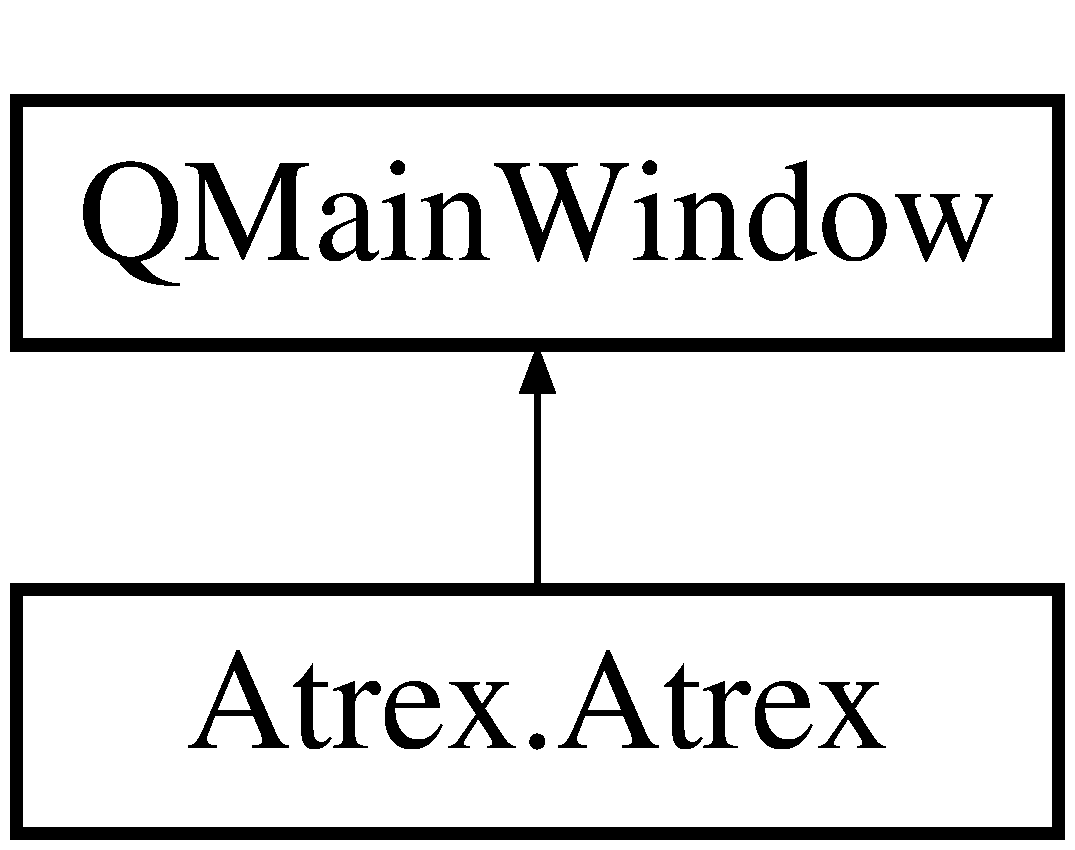
\includegraphics[height=2.000000cm]{class_atrex_1_1_atrex}
\end{center}
\end{figure}
\subsection*{Public Member Functions}
\begin{DoxyCompactItemize}
\item 
def \hyperlink{class_atrex_1_1_atrex_a3c7c6f6088f83b942d6773648e1e6347}{\-\_\-\-\_\-init\-\_\-\-\_\-}
\begin{DoxyCompactList}\small\item\em init -\/ Constructor for the atrex class. \end{DoxyCompactList}\item 
def \hyperlink{class_atrex_1_1_atrex_a6877cdfc8717ffc47d5e25a7fa1385f3}{get\-Home}
\begin{DoxyCompactList}\small\item\em get\-Home get the user's home directory \end{DoxyCompactList}\item 
def \hyperlink{class_atrex_1_1_atrex_a500ea9d7087f2aaf505f87998d1cf526}{close\-Event}
\begin{DoxyCompactList}\small\item\em close\-Event shut down the program cleanly \end{DoxyCompactList}\item 
def \hyperlink{class_atrex_1_1_atrex_aab80061d4d2127e82b592cbf5baef054}{open\-Image}
\begin{DoxyCompactList}\small\item\em open\-Image method to open an image, will query the user via an Q\-File\-Dialog \end{DoxyCompactList}\item 
def \hyperlink{class_atrex_1_1_atrex_a25ef435a888471b35045f63fad55b176}{open\-Image\-File}
\begin{DoxyCompactList}\small\item\em open\-Image\-File method to open an image \end{DoxyCompactList}\item 
def \hyperlink{class_atrex_1_1_atrex_ab96f78f24269b2608673faa9cec31ad8}{peak\-Box\-Size\-Set}
\item 
def \hyperlink{class_atrex_1_1_atrex_a02d26a480697d4631d2d8d2c76567a5b}{zoom\-Fac\-Update}
\item 
def \hyperlink{class_atrex_1_1_atrex_ab94534c12f07a7fcce69bbfc8a175692}{new\-Cent}
\item 
def \hyperlink{class_atrex_1_1_atrex_a3031c6519f2f84e9eee3a482f27132cc}{new\-Zm\-Box}
\item 
def \hyperlink{class_atrex_1_1_atrex_a64c7ac662276466211b6d02b2ad9d430}{disp\-Min\-Pressed}
\item 
def \hyperlink{class_atrex_1_1_atrex_add0fa0a0b9345510d0cf8d834e3734dd}{disp\-Max\-Pressed}
\item 
def \hyperlink{class_atrex_1_1_atrex_a2b706eddbe63823363f801bb0878eb44}{update\-Image}
\item 
def \hyperlink{class_atrex_1_1_atrex_aa8435a0f0357634c9180d2fd4aa5ce75}{imtype\-Changed}
\item 
def \hyperlink{class_atrex_1_1_atrex_ada591cc2d1c26152ddbaf72f7f7efc4c}{new\-Slider\-Value}
\item 
def \hyperlink{class_atrex_1_1_atrex_a9db0c9087a9c3adbb07b2e887322941e}{decrement\-Image\-Value}
\item 
def \hyperlink{class_atrex_1_1_atrex_aa766d95d2be1bd5b466da0a2581ca0e5}{increment\-Image\-Value}
\item 
def \hyperlink{class_atrex_1_1_atrex_acd608751b80f2f6e38b8e3a3c804aba6}{new\-Image\-Value}
\item 
def \hyperlink{class_atrex_1_1_atrex_ae474912922a15f4c46cfa4b81c6428d4}{max\-Slider\-Update}
\item 
def \hyperlink{class_atrex_1_1_atrex_ada41f153ca507e3f48294d042e991a79}{minmax\-D\-N\-Slider\-Released}
\item 
def \hyperlink{class_atrex_1_1_atrex_aec14907b3f14a48f9805194cd196b67c}{min\-Slider\-Update}
\item 
def \hyperlink{class_atrex_1_1_atrex_aae57dd8400942b0f992b4c4bc868da64}{lut\-Changed}
\item 
def \hyperlink{class_atrex_1_1_atrex_af3b9d9a660caa590a68da51656d622fb}{def\-Image\-Dir}
\item 
def \hyperlink{class_atrex_1_1_atrex_aca19dbda20686dcaef166d9680528e21}{def\-Work\-Dir}
\item 
def \hyperlink{class_atrex_1_1_atrex_ac995f1abf16ed66fea8a907373ff9475}{image\-Mouse\-Clicked}
\item 
def \hyperlink{class_atrex_1_1_atrex_adc2b173f9b80955c6f4fc7a156e9d091}{display\-Cake\-Image}
\item 
def \hyperlink{class_atrex_1_1_atrex_abfe78ab11ed54f2e83bb9fddfb16a573}{display\-Image}
\item 
def \hyperlink{class_atrex_1_1_atrex_a101abfd070fc8f268fb07c79026d778e}{new\-Peak}
\item 
def \hyperlink{class_atrex_1_1_atrex_a8778bbe32534eadb568016f2de735ef2}{update\-Peaks}
\item 
def \hyperlink{class_atrex_1_1_atrex_a88cac9434ce28cbff05cb12b81023d4d}{update\-Peak\-List}
\item 
def \hyperlink{class_atrex_1_1_atrex_a2452575598eb0088e452b2160610da4f}{peak\-List\-Clicked}
\begin{DoxyCompactList}\small\item\em peak\-List\-C\-Licked \end{DoxyCompactList}\item 
def \hyperlink{class_atrex_1_1_atrex_ace2289de8cacf431113b0a06133c5693}{adjust\-Peak\-Displays}
\item 
def \hyperlink{class_atrex_1_1_atrex_a17585a5304b57ea95ad13e6feeebbcde}{list\-Button\-Changed}
\item 
def \hyperlink{class_atrex_1_1_atrex_a245293bfb74e32de50e99de66ffeeb55}{load\-Fit\-Params}
\item 
def \hyperlink{class_atrex_1_1_atrex_a054de9d87526f2849d35862b6747a658}{zoom\-Mode}
\item 
def \hyperlink{class_atrex_1_1_atrex_a0efd15d4cccf12a54b9263d84dca6d42}{add\-Peak\-Mode}
\item 
def \hyperlink{class_atrex_1_1_atrex_a99248a89609473aaf887150c69e087fd}{select\-Mode}
\item 
def \hyperlink{class_atrex_1_1_atrex_a739717834e7626d1ba9a1986430f7cf4}{unselect\-Mode}
\item 
def \hyperlink{class_atrex_1_1_atrex_af107ee890ef60784ad28314a7908c439}{mask\-Mode}
\item 
def \hyperlink{class_atrex_1_1_atrex_a45a6a72900b8977bc8497f0ad2c0314a}{unmask\-Mode}
\item 
def \hyperlink{class_atrex_1_1_atrex_a96817ca44885b91f7d2ba9cbff61ced5}{select\-Rect}
\item 
def \hyperlink{class_atrex_1_1_atrex_a210da0549837b917dbb10bd194704d67}{mask\-Rect}
\item 
def \hyperlink{class_atrex_1_1_atrex_a4dce042d175e3f9593319481166886fd}{clear\-Mask}
\item 
def \hyperlink{class_atrex_1_1_atrex_a9a254e4f37cfc3286bab09e45de45db8}{save\-Mask}
\item 
def \hyperlink{class_atrex_1_1_atrex_a3edba6d33e67d7c8cf3eace6aa7bcb1a}{read\-Mask}
\item 
def \hyperlink{class_atrex_1_1_atrex_ac50dc26f3143315895b9afe212aeaa27}{sel\-All\-Peaks}
\item 
def \hyperlink{class_atrex_1_1_atrex_aaf655985f170b76903e840bae4cae564}{clear\-All\-Peaks}
\item 
def \hyperlink{class_atrex_1_1_atrex_a1b95e20242dba81dce9ed56aa33d4502}{move\-Sel\-Peaks}
\item 
def \hyperlink{class_atrex_1_1_atrex_ab8dacb09c6a0a632de6bccdc77836dec}{Remove\-All\-Peaks}
\item 
def \hyperlink{class_atrex_1_1_atrex_a3d1ea171a1570456260a8c9e1ff61f2e}{del\-Sel\-Peaks}
\item 
def \hyperlink{class_atrex_1_1_atrex_a7577e8ee32a4909dde0cdc26cec42439}{set\-Buttons}
\item 
def \hyperlink{class_atrex_1_1_atrex_a3ba5414e1ff2fd707ee5aa923371e917}{update\-Peak\-Number\-L\-E}
\item 
def \hyperlink{class_atrex_1_1_atrex_aed5e2cfdb3aa93f0b93f5f92923c10b6}{open\-Detector\-Calibration}
\item 
def \hyperlink{class_atrex_1_1_atrex_a6ddf6ff6c06c18493233eb34db019ac6}{save\-Detector\-Calibration}
\item 
def \hyperlink{class_atrex_1_1_atrex_a33ff7708e43d3f78a0da47e2740b783a}{Display\-\_\-\-Detector\-\_\-calibration}
\item 
def \hyperlink{class_atrex_1_1_atrex_abddae09c11c780c9f83fa74a693e3244}{Update\-\_\-\-Detector\-\_\-calibration}
\item 
def \hyperlink{class_atrex_1_1_atrex_a99527243c5cb42e343391bbd921321f0}{Search\-For\-Peaks}
\item 
def \hyperlink{class_atrex_1_1_atrex_aa44defd7fc02dad7f4371e2a2eccf710}{Search\-For\-Peaks\-Series}
\item 
def \hyperlink{class_atrex_1_1_atrex_a816143e04438e686d80a2172cb484f44}{merge\-Cancel}
\item 
def \hyperlink{class_atrex_1_1_atrex_acc559ce6fbdf2cb95ada0b191ced0c04}{merge\-Image\-Range}
\item 
def \hyperlink{class_atrex_1_1_atrex_aff22266d12cc6092353a9e53081edb9d}{Save\-Peak\-Table}
\item 
def \hyperlink{class_atrex_1_1_atrex_af2a8d53b7aa4d5211b9eb3ac25045501}{Open\-Peak\-Table}
\item 
def \hyperlink{class_atrex_1_1_atrex_aa996a3132c9ace217efe5826349df1df}{Peak\-List\-Browse}
\item 
def \hyperlink{class_atrex_1_1_atrex_a5e8c4a39fedb7dff274082c2b7cc352f}{read\-Text\-Detect}
\item 
def \hyperlink{class_atrex_1_1_atrex_a0545caa06d0d5297147a325e9f2763c5}{write\-Text\-Detect}
\item 
def \hyperlink{class_atrex_1_1_atrex_ac277ee5f02ff03bf577c91d2351d3833}{update\-Plot}
\item 
def \hyperlink{class_atrex_1_1_atrex_a5380dd3e2db37a9e6316dcfb2f79da52}{save\-Plot\-To\-File}
\item 
def \hyperlink{class_atrex_1_1_atrex_a51c8994be54b7062fd0b7cc077783f52}{plot\-X\-Y\-From\-File}
\item 
def \hyperlink{class_atrex_1_1_atrex_a4125657b083972e131da1e06587af07f}{overlay\-Plot\-From\-File}
\item 
def \hyperlink{class_atrex_1_1_atrex_a3946e847c41ffc83f4fee8787b1449a7}{read\-X\-P\-O\-W}
\item 
def \hyperlink{class_atrex_1_1_atrex_a82e4c50e20fab4518b71703bdde02994}{read\-J\-C\-P\-D\-S}
\item 
def \hyperlink{class_atrex_1_1_atrex_a4a1adbdba785016117f258c281895688}{int\-Current}
\item 
def \hyperlink{class_atrex_1_1_atrex_a4ed5b63695c617a40eb6fc2c50db7575}{cake\-Current}
\item 
def \hyperlink{class_atrex_1_1_atrex_aa1141a78fc819e7fd22a44e1847a89ba}{test\-Calc}
\item 
def \hyperlink{class_atrex_1_1_atrex_aaa0ad76fcdcdde4e7138ade95031e6c7}{calc2theta}
\item 
def \hyperlink{class_atrex_1_1_atrex_ac75d2b26897d6d799773b27b41ea369b}{done2theta}
\item 
def \hyperlink{class_atrex_1_1_atrex_a4d6871d5055309cbbaddb62e00bfbea5}{peak\-File\-Browse}
\item 
def \hyperlink{class_atrex_1_1_atrex_aaa23b7529d44f3cbbeedfd8434c8bce9}{peak\-Save\-To\-File}
\item 
def \hyperlink{class_atrex_1_1_atrex_a3a5f2aee5b962e1615c54395d9edd172}{plot\-Peak\-Prof}
\begin{DoxyCompactList}\small\item\em Function to plot the vertical or horizontal profile of the peak Vert flag controlled by combo-\/box selection This is only for first time, when vbar or hbar is centered on the image. \end{DoxyCompactList}\item 
def \hyperlink{class_atrex_1_1_atrex_ad7997e5a735ce1b34d713a4b27490fbc}{new\-Peak\-Prof\-Location}
\item 
def \hyperlink{class_atrex_1_1_atrex_a31041eb876dff6083a13777f44d09274}{peak\-Prof\-Orientation\-Set}
\item 
def \hyperlink{class_atrex_1_1_atrex_a8ed3b24c6fdcc06364436368a5112f77}{read\-Predict\-Settings}
\item 
def \hyperlink{class_atrex_1_1_atrex_ad59de2bb679492d17867acb6fffa534e}{start\-Simulate}
\item 
def \hyperlink{class_atrex_1_1_atrex_a9c7db3ee59b336c77f361177d0d14248}{update\-Display}
\item 
def \hyperlink{class_atrex_1_1_atrex_a74436efac3bb11530dbab592fe41c352}{read\-\_\-box\-\_\-change}
\item 
def \hyperlink{class_atrex_1_1_atrex_a8201adc7c4c0956f9adc65b9abdf8172}{get\-Cal\-Peaks}
\end{DoxyCompactItemize}
\subsection*{Public Attributes}
\begin{DoxyCompactItemize}
\item 
\hyperlink{class_atrex_1_1_atrex_a35cabdfa4a6164da07e19c4b4ed957aa}{ui}
\item 
\hyperlink{class_atrex_1_1_atrex_aba7d9d2058a5bdace86c305ecd35ad3b}{work\-Directory}
\item 
\hyperlink{class_atrex_1_1_atrex_a3a5510d39868ddfaae38841e8057394a}{image\-Directory}
\item 
\hyperlink{class_atrex_1_1_atrex_a6c50fb1f9133397ae0936d14310edabd}{image\-File}
\item 
\hyperlink{class_atrex_1_1_atrex_ac6283b2b56309698f9b3881fd1cb0ba2}{detect\-File}
\item 
\hyperlink{class_atrex_1_1_atrex_adee5f16f849c0990481863170787811e}{myim}
\item 
\hyperlink{class_atrex_1_1_atrex_a7f2c3002d88c2f13aa3f0f19899a0ab7}{zm\-Cent\-Loc}
\item 
\hyperlink{class_atrex_1_1_atrex_a845e289d7ed3657f89da88d1d53657bc}{active\-List}
\item 
\hyperlink{class_atrex_1_1_atrex_a1fd77da8e55fec3336694f7817bb6cb2}{peaks}
\item 
\hyperlink{class_atrex_1_1_atrex_ad1a660b6c6750e5d21a4c51abffbb2df}{peaks0}
\item 
\hyperlink{class_atrex_1_1_atrex_ace3b741c1a559e2117246a53d3e8f345}{peaks1}
\item 
\hyperlink{class_atrex_1_1_atrex_a47354f98e68c5aadcd988d0a2b476889}{detector}
\item 
\hyperlink{class_atrex_1_1_atrex_a7efc2659254ab5a5f065a5f3fa11ceb9}{fitarr}
\begin{DoxyCompactList}\small\item\em .ui.\-zoom\-Tab\-Widgets.\-set\-Current\-Index(0) \end{DoxyCompactList}\item 
\hyperlink{class_atrex_1_1_atrex_a804307169058c96d52235bacc92d6f09}{param\-File}
\item 
\hyperlink{class_atrex_1_1_atrex_a2080a9ed5c4661217ebd6fa108ef2e68}{base}
\item 
\hyperlink{class_atrex_1_1_atrex_a8cb32e63ba2e1df2a5819e6df5bfd8e9}{min\-Range}
\item 
\hyperlink{class_atrex_1_1_atrex_a240f5adcbd64d4282c41fc884722d453}{max\-Range}
\item 
\hyperlink{class_atrex_1_1_atrex_ac181165f963c93be5b4a5e79ac9100e2}{imtype\-Flag}
\item 
\hyperlink{class_atrex_1_1_atrex_aaad2acdd3e1ed0343b2414934ce8c257}{imsize}
\begin{DoxyCompactList}\small\item\em read in the accompanying settings file for the image if it exists \end{DoxyCompactList}\item 
\hyperlink{class_atrex_1_1_atrex_a46922869bb36221d04b4723afc6ceded}{myproj}
\item 
\hyperlink{class_atrex_1_1_atrex_a5a00bf83d75cef3dc64f66b7972128ac}{old\-Selected}
\item 
\hyperlink{class_atrex_1_1_atrex_a9db3f47f57f62dedb23235d73c5b81c7}{peak\-Startx}
\item 
\hyperlink{class_atrex_1_1_atrex_a7128a7471ca115d494fb8457397cb3b4}{peak\-Starty}
\item 
\hyperlink{class_atrex_1_1_atrex_a9ddce163f1008e4421d95874f8a7e006}{select\-Peak\-X\-Y}
\item 
\hyperlink{class_atrex_1_1_atrex_a5034cf92d78b203761c82c2d09571fe7}{cancel\-Merge}
\item 
\hyperlink{class_atrex_1_1_atrex_ac308bffb51e8c4a11b2adbbaf85e38ec}{mysim}
\end{DoxyCompactItemize}
\subsection*{Static Public Attributes}
\begin{DoxyCompactItemize}
\item 
\hyperlink{class_atrex_1_1_atrex_adb81a9472392a89ed733d7d0779e45b7}{displayed\-Image} = False
\item 
int \hyperlink{class_atrex_1_1_atrex_ae832c8b0566a3106d3021b88ea739683}{min\-Range} = 1
\item 
int \hyperlink{class_atrex_1_1_atrex_ad050fe0947cfc2aaed121ca1f306d637}{max\-Range} = 99
\item 
\hyperlink{class_atrex_1_1_atrex_a68605f5249c1a23ea96180aa7c011acd}{merge\-Sum\-Mode} = True
\item 
tuple \hyperlink{class_atrex_1_1_atrex_af008dc7c13f040fea0e0bd315badd461}{mymask} = \hyperlink{classmy_mask_1_1my_mask}{my\-Mask}()
\item 
tuple \hyperlink{class_atrex_1_1_atrex_af1384190082613188d50f79e7dacb4d4}{mypred} = \hyperlink{classmy_predict_1_1my_predict}{my\-Predict}()
\item 
string \hyperlink{class_atrex_1_1_atrex_a6c119a7ed751e933a34e165078520474}{olay\-File} = \char`\"{}\char`\"{}
\item 
\hyperlink{class_atrex_1_1_atrex_a2ae7c7ded99e983cf654f68a09974198}{olay\-Sec\-Flag} = False
\item 
\hyperlink{class_atrex_1_1_atrex_a227e61447cc5900a7a818713fffb4d9e}{first\-Display} = True
\item 
int \hyperlink{class_atrex_1_1_atrex_aabc4d80436aab113d3ecabc4fb692c8e}{imtype\-Flag} = 0
\item 
list \hyperlink{class_atrex_1_1_atrex_aec9ff4f8500b49c9d93872db1a458c5e}{select\-Peak\-X\-Y} = \mbox{[}0.,0.\mbox{]}
\item 
tuple \hyperlink{class_atrex_1_1_atrex_ab1b2d6a17f54b2f004daea4b71512152}{imsize} = (0,0)
\item 
int \hyperlink{class_atrex_1_1_atrex_a6d1d3398ca810ec9843f350350736793}{peak\-Box\-Size} = 33
\item 
int \hyperlink{class_atrex_1_1_atrex_ad74b4f1510f5797e76342de65eaf8433}{old\-Selected} = -\/1
\item 
\hyperlink{class_atrex_1_1_atrex_a4ca8a779dc0d0c890538d52bf28dd7da}{vert\-Prof\-Flag} = True
\item 
int \hyperlink{class_atrex_1_1_atrex_a8131137cca435bd72d5a9080f758c0ae}{peak\-Startx} = 0
\item 
int \hyperlink{class_atrex_1_1_atrex_a52f02e7771533226a5289d5ad149b71e}{peak\-Starty} = 0
\item 
\hyperlink{class_atrex_1_1_atrex_ac11efcc7aecf0e1378a6ea2403695cd9}{merge\-Arr} = None
\item 
\hyperlink{class_atrex_1_1_atrex_ab8f629b3d4108ac9fb6bf240b3f08a33}{merge\-File\-Name} = None
\item 
\hyperlink{class_atrex_1_1_atrex_a1f1c13bd2ef993ce756a84f7cd7448f7}{merge\-Display\-Flag} = False
\item 
\hyperlink{class_atrex_1_1_atrex_a6e11d4a775a3fbcca2fc6cb4f01963eb}{image\-File\-Pref} = None
\item 
tuple \hyperlink{class_atrex_1_1_atrex_a9db69c9f42cd99180c0ce16fab4f4502}{myproj} = \hyperlink{class_project_1_1_project}{Project}()
\end{DoxyCompactItemize}


\subsection{Detailed Description}
\hyperlink{class_atrex_1_1_atrex}{Atrex} Top level class of the \hyperlink{class_atrex_1_1_atrex}{Atrex} software package. 

Loads ui\-Main\-Win.\-ui and handles all events generated by the ui. This is the main control class of the \hyperlink{class_atrex_1_1_atrex}{Atrex} package. 

\subsection{Constructor \& Destructor Documentation}
\hypertarget{class_atrex_1_1_atrex_a3c7c6f6088f83b942d6773648e1e6347}{\index{Atrex\-::\-Atrex@{Atrex\-::\-Atrex}!\-\_\-\-\_\-init\-\_\-\-\_\-@{\-\_\-\-\_\-init\-\_\-\-\_\-}}
\index{\-\_\-\-\_\-init\-\_\-\-\_\-@{\-\_\-\-\_\-init\-\_\-\-\_\-}!Atrex::Atrex@{Atrex\-::\-Atrex}}
\subsubsection[{\-\_\-\-\_\-init\-\_\-\-\_\-}]{\setlength{\rightskip}{0pt plus 5cm}def Atrex.\-Atrex.\-\_\-\-\_\-init\-\_\-\-\_\- (
\begin{DoxyParamCaption}
\item[{}]{self}
\end{DoxyParamCaption}
)}}\label{class_atrex_1_1_atrex_a3c7c6f6088f83b942d6773648e1e6347}


init -\/ Constructor for the atrex class. 

initialize the gui controls, hook signals to slots 

\subsection{Member Function Documentation}
\hypertarget{class_atrex_1_1_atrex_a0efd15d4cccf12a54b9263d84dca6d42}{\index{Atrex\-::\-Atrex@{Atrex\-::\-Atrex}!add\-Peak\-Mode@{add\-Peak\-Mode}}
\index{add\-Peak\-Mode@{add\-Peak\-Mode}!Atrex::Atrex@{Atrex\-::\-Atrex}}
\subsubsection[{add\-Peak\-Mode}]{\setlength{\rightskip}{0pt plus 5cm}def Atrex.\-Atrex.\-add\-Peak\-Mode (
\begin{DoxyParamCaption}
\item[{}]{self}
\end{DoxyParamCaption}
)}}\label{class_atrex_1_1_atrex_a0efd15d4cccf12a54b9263d84dca6d42}
\hypertarget{class_atrex_1_1_atrex_ace2289de8cacf431113b0a06133c5693}{\index{Atrex\-::\-Atrex@{Atrex\-::\-Atrex}!adjust\-Peak\-Displays@{adjust\-Peak\-Displays}}
\index{adjust\-Peak\-Displays@{adjust\-Peak\-Displays}!Atrex::Atrex@{Atrex\-::\-Atrex}}
\subsubsection[{adjust\-Peak\-Displays}]{\setlength{\rightskip}{0pt plus 5cm}def Atrex.\-Atrex.\-adjust\-Peak\-Displays (
\begin{DoxyParamCaption}
\item[{}]{self}
\end{DoxyParamCaption}
)}}\label{class_atrex_1_1_atrex_ace2289de8cacf431113b0a06133c5693}
\hypertarget{class_atrex_1_1_atrex_a4ed5b63695c617a40eb6fc2c50db7575}{\index{Atrex\-::\-Atrex@{Atrex\-::\-Atrex}!cake\-Current@{cake\-Current}}
\index{cake\-Current@{cake\-Current}!Atrex::Atrex@{Atrex\-::\-Atrex}}
\subsubsection[{cake\-Current}]{\setlength{\rightskip}{0pt plus 5cm}def Atrex.\-Atrex.\-cake\-Current (
\begin{DoxyParamCaption}
\item[{}]{self}
\end{DoxyParamCaption}
)}}\label{class_atrex_1_1_atrex_a4ed5b63695c617a40eb6fc2c50db7575}
\hypertarget{class_atrex_1_1_atrex_aaa0ad76fcdcdde4e7138ade95031e6c7}{\index{Atrex\-::\-Atrex@{Atrex\-::\-Atrex}!calc2theta@{calc2theta}}
\index{calc2theta@{calc2theta}!Atrex::Atrex@{Atrex\-::\-Atrex}}
\subsubsection[{calc2theta}]{\setlength{\rightskip}{0pt plus 5cm}def Atrex.\-Atrex.\-calc2theta (
\begin{DoxyParamCaption}
\item[{}]{self}
\end{DoxyParamCaption}
)}}\label{class_atrex_1_1_atrex_aaa0ad76fcdcdde4e7138ade95031e6c7}
\hypertarget{class_atrex_1_1_atrex_aaf655985f170b76903e840bae4cae564}{\index{Atrex\-::\-Atrex@{Atrex\-::\-Atrex}!clear\-All\-Peaks@{clear\-All\-Peaks}}
\index{clear\-All\-Peaks@{clear\-All\-Peaks}!Atrex::Atrex@{Atrex\-::\-Atrex}}
\subsubsection[{clear\-All\-Peaks}]{\setlength{\rightskip}{0pt plus 5cm}def Atrex.\-Atrex.\-clear\-All\-Peaks (
\begin{DoxyParamCaption}
\item[{}]{self}
\end{DoxyParamCaption}
)}}\label{class_atrex_1_1_atrex_aaf655985f170b76903e840bae4cae564}
\hypertarget{class_atrex_1_1_atrex_a4dce042d175e3f9593319481166886fd}{\index{Atrex\-::\-Atrex@{Atrex\-::\-Atrex}!clear\-Mask@{clear\-Mask}}
\index{clear\-Mask@{clear\-Mask}!Atrex::Atrex@{Atrex\-::\-Atrex}}
\subsubsection[{clear\-Mask}]{\setlength{\rightskip}{0pt plus 5cm}def Atrex.\-Atrex.\-clear\-Mask (
\begin{DoxyParamCaption}
\item[{}]{self}
\end{DoxyParamCaption}
)}}\label{class_atrex_1_1_atrex_a4dce042d175e3f9593319481166886fd}
\hypertarget{class_atrex_1_1_atrex_a500ea9d7087f2aaf505f87998d1cf526}{\index{Atrex\-::\-Atrex@{Atrex\-::\-Atrex}!close\-Event@{close\-Event}}
\index{close\-Event@{close\-Event}!Atrex::Atrex@{Atrex\-::\-Atrex}}
\subsubsection[{close\-Event}]{\setlength{\rightskip}{0pt plus 5cm}def Atrex.\-Atrex.\-close\-Event (
\begin{DoxyParamCaption}
\item[{}]{self, }
\item[{}]{event}
\end{DoxyParamCaption}
)}}\label{class_atrex_1_1_atrex_a500ea9d7087f2aaf505f87998d1cf526}


close\-Event shut down the program cleanly 

\hypertarget{class_atrex_1_1_atrex_a9db0c9087a9c3adbb07b2e887322941e}{\index{Atrex\-::\-Atrex@{Atrex\-::\-Atrex}!decrement\-Image\-Value@{decrement\-Image\-Value}}
\index{decrement\-Image\-Value@{decrement\-Image\-Value}!Atrex::Atrex@{Atrex\-::\-Atrex}}
\subsubsection[{decrement\-Image\-Value}]{\setlength{\rightskip}{0pt plus 5cm}def Atrex.\-Atrex.\-decrement\-Image\-Value (
\begin{DoxyParamCaption}
\item[{}]{self}
\end{DoxyParamCaption}
)}}\label{class_atrex_1_1_atrex_a9db0c9087a9c3adbb07b2e887322941e}
\hypertarget{class_atrex_1_1_atrex_af3b9d9a660caa590a68da51656d622fb}{\index{Atrex\-::\-Atrex@{Atrex\-::\-Atrex}!def\-Image\-Dir@{def\-Image\-Dir}}
\index{def\-Image\-Dir@{def\-Image\-Dir}!Atrex::Atrex@{Atrex\-::\-Atrex}}
\subsubsection[{def\-Image\-Dir}]{\setlength{\rightskip}{0pt plus 5cm}def Atrex.\-Atrex.\-def\-Image\-Dir (
\begin{DoxyParamCaption}
\item[{}]{self}
\end{DoxyParamCaption}
)}}\label{class_atrex_1_1_atrex_af3b9d9a660caa590a68da51656d622fb}
\hypertarget{class_atrex_1_1_atrex_aca19dbda20686dcaef166d9680528e21}{\index{Atrex\-::\-Atrex@{Atrex\-::\-Atrex}!def\-Work\-Dir@{def\-Work\-Dir}}
\index{def\-Work\-Dir@{def\-Work\-Dir}!Atrex::Atrex@{Atrex\-::\-Atrex}}
\subsubsection[{def\-Work\-Dir}]{\setlength{\rightskip}{0pt plus 5cm}def Atrex.\-Atrex.\-def\-Work\-Dir (
\begin{DoxyParamCaption}
\item[{}]{self}
\end{DoxyParamCaption}
)}}\label{class_atrex_1_1_atrex_aca19dbda20686dcaef166d9680528e21}
\hypertarget{class_atrex_1_1_atrex_a3d1ea171a1570456260a8c9e1ff61f2e}{\index{Atrex\-::\-Atrex@{Atrex\-::\-Atrex}!del\-Sel\-Peaks@{del\-Sel\-Peaks}}
\index{del\-Sel\-Peaks@{del\-Sel\-Peaks}!Atrex::Atrex@{Atrex\-::\-Atrex}}
\subsubsection[{del\-Sel\-Peaks}]{\setlength{\rightskip}{0pt plus 5cm}def Atrex.\-Atrex.\-del\-Sel\-Peaks (
\begin{DoxyParamCaption}
\item[{}]{self}
\end{DoxyParamCaption}
)}}\label{class_atrex_1_1_atrex_a3d1ea171a1570456260a8c9e1ff61f2e}
\hypertarget{class_atrex_1_1_atrex_a33ff7708e43d3f78a0da47e2740b783a}{\index{Atrex\-::\-Atrex@{Atrex\-::\-Atrex}!Display\-\_\-\-Detector\-\_\-calibration@{Display\-\_\-\-Detector\-\_\-calibration}}
\index{Display\-\_\-\-Detector\-\_\-calibration@{Display\-\_\-\-Detector\-\_\-calibration}!Atrex::Atrex@{Atrex\-::\-Atrex}}
\subsubsection[{Display\-\_\-\-Detector\-\_\-calibration}]{\setlength{\rightskip}{0pt plus 5cm}def Atrex.\-Atrex.\-Display\-\_\-\-Detector\-\_\-calibration (
\begin{DoxyParamCaption}
\item[{}]{self, }
\item[{}]{det}
\end{DoxyParamCaption}
)}}\label{class_atrex_1_1_atrex_a33ff7708e43d3f78a0da47e2740b783a}
\hypertarget{class_atrex_1_1_atrex_adc2b173f9b80955c6f4fc7a156e9d091}{\index{Atrex\-::\-Atrex@{Atrex\-::\-Atrex}!display\-Cake\-Image@{display\-Cake\-Image}}
\index{display\-Cake\-Image@{display\-Cake\-Image}!Atrex::Atrex@{Atrex\-::\-Atrex}}
\subsubsection[{display\-Cake\-Image}]{\setlength{\rightskip}{0pt plus 5cm}def Atrex.\-Atrex.\-display\-Cake\-Image (
\begin{DoxyParamCaption}
\item[{}]{self}
\end{DoxyParamCaption}
)}}\label{class_atrex_1_1_atrex_adc2b173f9b80955c6f4fc7a156e9d091}
\hypertarget{class_atrex_1_1_atrex_abfe78ab11ed54f2e83bb9fddfb16a573}{\index{Atrex\-::\-Atrex@{Atrex\-::\-Atrex}!display\-Image@{display\-Image}}
\index{display\-Image@{display\-Image}!Atrex::Atrex@{Atrex\-::\-Atrex}}
\subsubsection[{display\-Image}]{\setlength{\rightskip}{0pt plus 5cm}def Atrex.\-Atrex.\-display\-Image (
\begin{DoxyParamCaption}
\item[{}]{self, }
\item[{}]{filename}
\end{DoxyParamCaption}
)}}\label{class_atrex_1_1_atrex_abfe78ab11ed54f2e83bb9fddfb16a573}
\hypertarget{class_atrex_1_1_atrex_add0fa0a0b9345510d0cf8d834e3734dd}{\index{Atrex\-::\-Atrex@{Atrex\-::\-Atrex}!disp\-Max\-Pressed@{disp\-Max\-Pressed}}
\index{disp\-Max\-Pressed@{disp\-Max\-Pressed}!Atrex::Atrex@{Atrex\-::\-Atrex}}
\subsubsection[{disp\-Max\-Pressed}]{\setlength{\rightskip}{0pt plus 5cm}def Atrex.\-Atrex.\-disp\-Max\-Pressed (
\begin{DoxyParamCaption}
\item[{}]{self}
\end{DoxyParamCaption}
)}}\label{class_atrex_1_1_atrex_add0fa0a0b9345510d0cf8d834e3734dd}
\hypertarget{class_atrex_1_1_atrex_a64c7ac662276466211b6d02b2ad9d430}{\index{Atrex\-::\-Atrex@{Atrex\-::\-Atrex}!disp\-Min\-Pressed@{disp\-Min\-Pressed}}
\index{disp\-Min\-Pressed@{disp\-Min\-Pressed}!Atrex::Atrex@{Atrex\-::\-Atrex}}
\subsubsection[{disp\-Min\-Pressed}]{\setlength{\rightskip}{0pt plus 5cm}def Atrex.\-Atrex.\-disp\-Min\-Pressed (
\begin{DoxyParamCaption}
\item[{}]{self}
\end{DoxyParamCaption}
)}}\label{class_atrex_1_1_atrex_a64c7ac662276466211b6d02b2ad9d430}
\hypertarget{class_atrex_1_1_atrex_ac75d2b26897d6d799773b27b41ea369b}{\index{Atrex\-::\-Atrex@{Atrex\-::\-Atrex}!done2theta@{done2theta}}
\index{done2theta@{done2theta}!Atrex::Atrex@{Atrex\-::\-Atrex}}
\subsubsection[{done2theta}]{\setlength{\rightskip}{0pt plus 5cm}def Atrex.\-Atrex.\-done2theta (
\begin{DoxyParamCaption}
\item[{}]{self}
\end{DoxyParamCaption}
)}}\label{class_atrex_1_1_atrex_ac75d2b26897d6d799773b27b41ea369b}
\hypertarget{class_atrex_1_1_atrex_a8201adc7c4c0956f9adc65b9abdf8172}{\index{Atrex\-::\-Atrex@{Atrex\-::\-Atrex}!get\-Cal\-Peaks@{get\-Cal\-Peaks}}
\index{get\-Cal\-Peaks@{get\-Cal\-Peaks}!Atrex::Atrex@{Atrex\-::\-Atrex}}
\subsubsection[{get\-Cal\-Peaks}]{\setlength{\rightskip}{0pt plus 5cm}def Atrex.\-Atrex.\-get\-Cal\-Peaks (
\begin{DoxyParamCaption}
\item[{}]{self}
\end{DoxyParamCaption}
)}}\label{class_atrex_1_1_atrex_a8201adc7c4c0956f9adc65b9abdf8172}
\hypertarget{class_atrex_1_1_atrex_a6877cdfc8717ffc47d5e25a7fa1385f3}{\index{Atrex\-::\-Atrex@{Atrex\-::\-Atrex}!get\-Home@{get\-Home}}
\index{get\-Home@{get\-Home}!Atrex::Atrex@{Atrex\-::\-Atrex}}
\subsubsection[{get\-Home}]{\setlength{\rightskip}{0pt plus 5cm}def Atrex.\-Atrex.\-get\-Home (
\begin{DoxyParamCaption}
\item[{}]{self}
\end{DoxyParamCaption}
)}}\label{class_atrex_1_1_atrex_a6877cdfc8717ffc47d5e25a7fa1385f3}


get\-Home get the user's home directory 

\hypertarget{class_atrex_1_1_atrex_ac995f1abf16ed66fea8a907373ff9475}{\index{Atrex\-::\-Atrex@{Atrex\-::\-Atrex}!image\-Mouse\-Clicked@{image\-Mouse\-Clicked}}
\index{image\-Mouse\-Clicked@{image\-Mouse\-Clicked}!Atrex::Atrex@{Atrex\-::\-Atrex}}
\subsubsection[{image\-Mouse\-Clicked}]{\setlength{\rightskip}{0pt plus 5cm}def Atrex.\-Atrex.\-image\-Mouse\-Clicked (
\begin{DoxyParamCaption}
\item[{}]{self, }
\item[{}]{vals}
\end{DoxyParamCaption}
)}}\label{class_atrex_1_1_atrex_ac995f1abf16ed66fea8a907373ff9475}
\hypertarget{class_atrex_1_1_atrex_aa8435a0f0357634c9180d2fd4aa5ce75}{\index{Atrex\-::\-Atrex@{Atrex\-::\-Atrex}!imtype\-Changed@{imtype\-Changed}}
\index{imtype\-Changed@{imtype\-Changed}!Atrex::Atrex@{Atrex\-::\-Atrex}}
\subsubsection[{imtype\-Changed}]{\setlength{\rightskip}{0pt plus 5cm}def Atrex.\-Atrex.\-imtype\-Changed (
\begin{DoxyParamCaption}
\item[{}]{self, }
\item[{}]{index}
\end{DoxyParamCaption}
)}}\label{class_atrex_1_1_atrex_aa8435a0f0357634c9180d2fd4aa5ce75}
\hypertarget{class_atrex_1_1_atrex_aa766d95d2be1bd5b466da0a2581ca0e5}{\index{Atrex\-::\-Atrex@{Atrex\-::\-Atrex}!increment\-Image\-Value@{increment\-Image\-Value}}
\index{increment\-Image\-Value@{increment\-Image\-Value}!Atrex::Atrex@{Atrex\-::\-Atrex}}
\subsubsection[{increment\-Image\-Value}]{\setlength{\rightskip}{0pt plus 5cm}def Atrex.\-Atrex.\-increment\-Image\-Value (
\begin{DoxyParamCaption}
\item[{}]{self}
\end{DoxyParamCaption}
)}}\label{class_atrex_1_1_atrex_aa766d95d2be1bd5b466da0a2581ca0e5}
\hypertarget{class_atrex_1_1_atrex_a4a1adbdba785016117f258c281895688}{\index{Atrex\-::\-Atrex@{Atrex\-::\-Atrex}!int\-Current@{int\-Current}}
\index{int\-Current@{int\-Current}!Atrex::Atrex@{Atrex\-::\-Atrex}}
\subsubsection[{int\-Current}]{\setlength{\rightskip}{0pt plus 5cm}def Atrex.\-Atrex.\-int\-Current (
\begin{DoxyParamCaption}
\item[{}]{self}
\end{DoxyParamCaption}
)}}\label{class_atrex_1_1_atrex_a4a1adbdba785016117f258c281895688}
\hypertarget{class_atrex_1_1_atrex_a17585a5304b57ea95ad13e6feeebbcde}{\index{Atrex\-::\-Atrex@{Atrex\-::\-Atrex}!list\-Button\-Changed@{list\-Button\-Changed}}
\index{list\-Button\-Changed@{list\-Button\-Changed}!Atrex::Atrex@{Atrex\-::\-Atrex}}
\subsubsection[{list\-Button\-Changed}]{\setlength{\rightskip}{0pt plus 5cm}def Atrex.\-Atrex.\-list\-Button\-Changed (
\begin{DoxyParamCaption}
\item[{}]{self, }
\item[{}]{event}
\end{DoxyParamCaption}
)}}\label{class_atrex_1_1_atrex_a17585a5304b57ea95ad13e6feeebbcde}
\hypertarget{class_atrex_1_1_atrex_a245293bfb74e32de50e99de66ffeeb55}{\index{Atrex\-::\-Atrex@{Atrex\-::\-Atrex}!load\-Fit\-Params@{load\-Fit\-Params}}
\index{load\-Fit\-Params@{load\-Fit\-Params}!Atrex::Atrex@{Atrex\-::\-Atrex}}
\subsubsection[{load\-Fit\-Params}]{\setlength{\rightskip}{0pt plus 5cm}def Atrex.\-Atrex.\-load\-Fit\-Params (
\begin{DoxyParamCaption}
\item[{}]{self, }
\item[{}]{fit\-Params}
\end{DoxyParamCaption}
)}}\label{class_atrex_1_1_atrex_a245293bfb74e32de50e99de66ffeeb55}
\hypertarget{class_atrex_1_1_atrex_aae57dd8400942b0f992b4c4bc868da64}{\index{Atrex\-::\-Atrex@{Atrex\-::\-Atrex}!lut\-Changed@{lut\-Changed}}
\index{lut\-Changed@{lut\-Changed}!Atrex::Atrex@{Atrex\-::\-Atrex}}
\subsubsection[{lut\-Changed}]{\setlength{\rightskip}{0pt plus 5cm}def Atrex.\-Atrex.\-lut\-Changed (
\begin{DoxyParamCaption}
\item[{}]{self, }
\item[{}]{index}
\end{DoxyParamCaption}
)}}\label{class_atrex_1_1_atrex_aae57dd8400942b0f992b4c4bc868da64}
\hypertarget{class_atrex_1_1_atrex_af107ee890ef60784ad28314a7908c439}{\index{Atrex\-::\-Atrex@{Atrex\-::\-Atrex}!mask\-Mode@{mask\-Mode}}
\index{mask\-Mode@{mask\-Mode}!Atrex::Atrex@{Atrex\-::\-Atrex}}
\subsubsection[{mask\-Mode}]{\setlength{\rightskip}{0pt plus 5cm}def Atrex.\-Atrex.\-mask\-Mode (
\begin{DoxyParamCaption}
\item[{}]{self}
\end{DoxyParamCaption}
)}}\label{class_atrex_1_1_atrex_af107ee890ef60784ad28314a7908c439}
\hypertarget{class_atrex_1_1_atrex_a210da0549837b917dbb10bd194704d67}{\index{Atrex\-::\-Atrex@{Atrex\-::\-Atrex}!mask\-Rect@{mask\-Rect}}
\index{mask\-Rect@{mask\-Rect}!Atrex::Atrex@{Atrex\-::\-Atrex}}
\subsubsection[{mask\-Rect}]{\setlength{\rightskip}{0pt plus 5cm}def Atrex.\-Atrex.\-mask\-Rect (
\begin{DoxyParamCaption}
\item[{}]{self, }
\item[{}]{rect, }
\item[{}]{s\-Flag}
\end{DoxyParamCaption}
)}}\label{class_atrex_1_1_atrex_a210da0549837b917dbb10bd194704d67}
\hypertarget{class_atrex_1_1_atrex_ae474912922a15f4c46cfa4b81c6428d4}{\index{Atrex\-::\-Atrex@{Atrex\-::\-Atrex}!max\-Slider\-Update@{max\-Slider\-Update}}
\index{max\-Slider\-Update@{max\-Slider\-Update}!Atrex::Atrex@{Atrex\-::\-Atrex}}
\subsubsection[{max\-Slider\-Update}]{\setlength{\rightskip}{0pt plus 5cm}def Atrex.\-Atrex.\-max\-Slider\-Update (
\begin{DoxyParamCaption}
\item[{}]{self, }
\item[{}]{newval}
\end{DoxyParamCaption}
)}}\label{class_atrex_1_1_atrex_ae474912922a15f4c46cfa4b81c6428d4}
\hypertarget{class_atrex_1_1_atrex_a816143e04438e686d80a2172cb484f44}{\index{Atrex\-::\-Atrex@{Atrex\-::\-Atrex}!merge\-Cancel@{merge\-Cancel}}
\index{merge\-Cancel@{merge\-Cancel}!Atrex::Atrex@{Atrex\-::\-Atrex}}
\subsubsection[{merge\-Cancel}]{\setlength{\rightskip}{0pt plus 5cm}def Atrex.\-Atrex.\-merge\-Cancel (
\begin{DoxyParamCaption}
\item[{}]{self}
\end{DoxyParamCaption}
)}}\label{class_atrex_1_1_atrex_a816143e04438e686d80a2172cb484f44}
\hypertarget{class_atrex_1_1_atrex_acc559ce6fbdf2cb95ada0b191ced0c04}{\index{Atrex\-::\-Atrex@{Atrex\-::\-Atrex}!merge\-Image\-Range@{merge\-Image\-Range}}
\index{merge\-Image\-Range@{merge\-Image\-Range}!Atrex::Atrex@{Atrex\-::\-Atrex}}
\subsubsection[{merge\-Image\-Range}]{\setlength{\rightskip}{0pt plus 5cm}def Atrex.\-Atrex.\-merge\-Image\-Range (
\begin{DoxyParamCaption}
\item[{}]{self}
\end{DoxyParamCaption}
)}}\label{class_atrex_1_1_atrex_acc559ce6fbdf2cb95ada0b191ced0c04}
\hypertarget{class_atrex_1_1_atrex_ada41f153ca507e3f48294d042e991a79}{\index{Atrex\-::\-Atrex@{Atrex\-::\-Atrex}!minmax\-D\-N\-Slider\-Released@{minmax\-D\-N\-Slider\-Released}}
\index{minmax\-D\-N\-Slider\-Released@{minmax\-D\-N\-Slider\-Released}!Atrex::Atrex@{Atrex\-::\-Atrex}}
\subsubsection[{minmax\-D\-N\-Slider\-Released}]{\setlength{\rightskip}{0pt plus 5cm}def Atrex.\-Atrex.\-minmax\-D\-N\-Slider\-Released (
\begin{DoxyParamCaption}
\item[{}]{self}
\end{DoxyParamCaption}
)}}\label{class_atrex_1_1_atrex_ada41f153ca507e3f48294d042e991a79}
\hypertarget{class_atrex_1_1_atrex_aec14907b3f14a48f9805194cd196b67c}{\index{Atrex\-::\-Atrex@{Atrex\-::\-Atrex}!min\-Slider\-Update@{min\-Slider\-Update}}
\index{min\-Slider\-Update@{min\-Slider\-Update}!Atrex::Atrex@{Atrex\-::\-Atrex}}
\subsubsection[{min\-Slider\-Update}]{\setlength{\rightskip}{0pt plus 5cm}def Atrex.\-Atrex.\-min\-Slider\-Update (
\begin{DoxyParamCaption}
\item[{}]{self, }
\item[{}]{newval}
\end{DoxyParamCaption}
)}}\label{class_atrex_1_1_atrex_aec14907b3f14a48f9805194cd196b67c}
\hypertarget{class_atrex_1_1_atrex_a1b95e20242dba81dce9ed56aa33d4502}{\index{Atrex\-::\-Atrex@{Atrex\-::\-Atrex}!move\-Sel\-Peaks@{move\-Sel\-Peaks}}
\index{move\-Sel\-Peaks@{move\-Sel\-Peaks}!Atrex::Atrex@{Atrex\-::\-Atrex}}
\subsubsection[{move\-Sel\-Peaks}]{\setlength{\rightskip}{0pt plus 5cm}def Atrex.\-Atrex.\-move\-Sel\-Peaks (
\begin{DoxyParamCaption}
\item[{}]{self}
\end{DoxyParamCaption}
)}}\label{class_atrex_1_1_atrex_a1b95e20242dba81dce9ed56aa33d4502}
\hypertarget{class_atrex_1_1_atrex_ab94534c12f07a7fcce69bbfc8a175692}{\index{Atrex\-::\-Atrex@{Atrex\-::\-Atrex}!new\-Cent@{new\-Cent}}
\index{new\-Cent@{new\-Cent}!Atrex::Atrex@{Atrex\-::\-Atrex}}
\subsubsection[{new\-Cent}]{\setlength{\rightskip}{0pt plus 5cm}def Atrex.\-Atrex.\-new\-Cent (
\begin{DoxyParamCaption}
\item[{}]{self, }
\item[{}]{newloc}
\end{DoxyParamCaption}
)}}\label{class_atrex_1_1_atrex_ab94534c12f07a7fcce69bbfc8a175692}
\hypertarget{class_atrex_1_1_atrex_acd608751b80f2f6e38b8e3a3c804aba6}{\index{Atrex\-::\-Atrex@{Atrex\-::\-Atrex}!new\-Image\-Value@{new\-Image\-Value}}
\index{new\-Image\-Value@{new\-Image\-Value}!Atrex::Atrex@{Atrex\-::\-Atrex}}
\subsubsection[{new\-Image\-Value}]{\setlength{\rightskip}{0pt plus 5cm}def Atrex.\-Atrex.\-new\-Image\-Value (
\begin{DoxyParamCaption}
\item[{}]{self}
\end{DoxyParamCaption}
)}}\label{class_atrex_1_1_atrex_acd608751b80f2f6e38b8e3a3c804aba6}
\hypertarget{class_atrex_1_1_atrex_a101abfd070fc8f268fb07c79026d778e}{\index{Atrex\-::\-Atrex@{Atrex\-::\-Atrex}!new\-Peak@{new\-Peak}}
\index{new\-Peak@{new\-Peak}!Atrex::Atrex@{Atrex\-::\-Atrex}}
\subsubsection[{new\-Peak}]{\setlength{\rightskip}{0pt plus 5cm}def Atrex.\-Atrex.\-new\-Peak (
\begin{DoxyParamCaption}
\item[{}]{self, }
\item[{}]{pt}
\end{DoxyParamCaption}
)}}\label{class_atrex_1_1_atrex_a101abfd070fc8f268fb07c79026d778e}
\hypertarget{class_atrex_1_1_atrex_ad7997e5a735ce1b34d713a4b27490fbc}{\index{Atrex\-::\-Atrex@{Atrex\-::\-Atrex}!new\-Peak\-Prof\-Location@{new\-Peak\-Prof\-Location}}
\index{new\-Peak\-Prof\-Location@{new\-Peak\-Prof\-Location}!Atrex::Atrex@{Atrex\-::\-Atrex}}
\subsubsection[{new\-Peak\-Prof\-Location}]{\setlength{\rightskip}{0pt plus 5cm}def Atrex.\-Atrex.\-new\-Peak\-Prof\-Location (
\begin{DoxyParamCaption}
\item[{}]{self, }
\item[{}]{v\-Flag, }
\item[{}]{x, }
\item[{}]{y}
\end{DoxyParamCaption}
)}}\label{class_atrex_1_1_atrex_ad7997e5a735ce1b34d713a4b27490fbc}
\hypertarget{class_atrex_1_1_atrex_ada591cc2d1c26152ddbaf72f7f7efc4c}{\index{Atrex\-::\-Atrex@{Atrex\-::\-Atrex}!new\-Slider\-Value@{new\-Slider\-Value}}
\index{new\-Slider\-Value@{new\-Slider\-Value}!Atrex::Atrex@{Atrex\-::\-Atrex}}
\subsubsection[{new\-Slider\-Value}]{\setlength{\rightskip}{0pt plus 5cm}def Atrex.\-Atrex.\-new\-Slider\-Value (
\begin{DoxyParamCaption}
\item[{}]{self, }
\item[{}]{newval}
\end{DoxyParamCaption}
)}}\label{class_atrex_1_1_atrex_ada591cc2d1c26152ddbaf72f7f7efc4c}
\hypertarget{class_atrex_1_1_atrex_a3031c6519f2f84e9eee3a482f27132cc}{\index{Atrex\-::\-Atrex@{Atrex\-::\-Atrex}!new\-Zm\-Box@{new\-Zm\-Box}}
\index{new\-Zm\-Box@{new\-Zm\-Box}!Atrex::Atrex@{Atrex\-::\-Atrex}}
\subsubsection[{new\-Zm\-Box}]{\setlength{\rightskip}{0pt plus 5cm}def Atrex.\-Atrex.\-new\-Zm\-Box (
\begin{DoxyParamCaption}
\item[{}]{self, }
\item[{}]{zmrect}
\end{DoxyParamCaption}
)}}\label{class_atrex_1_1_atrex_a3031c6519f2f84e9eee3a482f27132cc}
\hypertarget{class_atrex_1_1_atrex_aed5e2cfdb3aa93f0b93f5f92923c10b6}{\index{Atrex\-::\-Atrex@{Atrex\-::\-Atrex}!open\-Detector\-Calibration@{open\-Detector\-Calibration}}
\index{open\-Detector\-Calibration@{open\-Detector\-Calibration}!Atrex::Atrex@{Atrex\-::\-Atrex}}
\subsubsection[{open\-Detector\-Calibration}]{\setlength{\rightskip}{0pt plus 5cm}def Atrex.\-Atrex.\-open\-Detector\-Calibration (
\begin{DoxyParamCaption}
\item[{}]{self}
\end{DoxyParamCaption}
)}}\label{class_atrex_1_1_atrex_aed5e2cfdb3aa93f0b93f5f92923c10b6}
\hypertarget{class_atrex_1_1_atrex_aab80061d4d2127e82b592cbf5baef054}{\index{Atrex\-::\-Atrex@{Atrex\-::\-Atrex}!open\-Image@{open\-Image}}
\index{open\-Image@{open\-Image}!Atrex::Atrex@{Atrex\-::\-Atrex}}
\subsubsection[{open\-Image}]{\setlength{\rightskip}{0pt plus 5cm}def Atrex.\-Atrex.\-open\-Image (
\begin{DoxyParamCaption}
\item[{}]{self}
\end{DoxyParamCaption}
)}}\label{class_atrex_1_1_atrex_aab80061d4d2127e82b592cbf5baef054}


open\-Image method to open an image, will query the user via an Q\-File\-Dialog 

\hypertarget{class_atrex_1_1_atrex_a25ef435a888471b35045f63fad55b176}{\index{Atrex\-::\-Atrex@{Atrex\-::\-Atrex}!open\-Image\-File@{open\-Image\-File}}
\index{open\-Image\-File@{open\-Image\-File}!Atrex::Atrex@{Atrex\-::\-Atrex}}
\subsubsection[{open\-Image\-File}]{\setlength{\rightskip}{0pt plus 5cm}def Atrex.\-Atrex.\-open\-Image\-File (
\begin{DoxyParamCaption}
\item[{}]{self, }
\item[{}]{filename}
\end{DoxyParamCaption}
)}}\label{class_atrex_1_1_atrex_a25ef435a888471b35045f63fad55b176}


open\-Image\-File method to open an image 


\begin{DoxyParams}{Parameters}
{\em filename} & name of file to open from this file the image base will be established. \\
\hline
\end{DoxyParams}
\hypertarget{class_atrex_1_1_atrex_af2a8d53b7aa4d5211b9eb3ac25045501}{\index{Atrex\-::\-Atrex@{Atrex\-::\-Atrex}!Open\-Peak\-Table@{Open\-Peak\-Table}}
\index{Open\-Peak\-Table@{Open\-Peak\-Table}!Atrex::Atrex@{Atrex\-::\-Atrex}}
\subsubsection[{Open\-Peak\-Table}]{\setlength{\rightskip}{0pt plus 5cm}def Atrex.\-Atrex.\-Open\-Peak\-Table (
\begin{DoxyParamCaption}
\item[{}]{self}
\end{DoxyParamCaption}
)}}\label{class_atrex_1_1_atrex_af2a8d53b7aa4d5211b9eb3ac25045501}
\hypertarget{class_atrex_1_1_atrex_a4125657b083972e131da1e06587af07f}{\index{Atrex\-::\-Atrex@{Atrex\-::\-Atrex}!overlay\-Plot\-From\-File@{overlay\-Plot\-From\-File}}
\index{overlay\-Plot\-From\-File@{overlay\-Plot\-From\-File}!Atrex::Atrex@{Atrex\-::\-Atrex}}
\subsubsection[{overlay\-Plot\-From\-File}]{\setlength{\rightskip}{0pt plus 5cm}def Atrex.\-Atrex.\-overlay\-Plot\-From\-File (
\begin{DoxyParamCaption}
\item[{}]{self}
\end{DoxyParamCaption}
)}}\label{class_atrex_1_1_atrex_a4125657b083972e131da1e06587af07f}
\hypertarget{class_atrex_1_1_atrex_ab96f78f24269b2608673faa9cec31ad8}{\index{Atrex\-::\-Atrex@{Atrex\-::\-Atrex}!peak\-Box\-Size\-Set@{peak\-Box\-Size\-Set}}
\index{peak\-Box\-Size\-Set@{peak\-Box\-Size\-Set}!Atrex::Atrex@{Atrex\-::\-Atrex}}
\subsubsection[{peak\-Box\-Size\-Set}]{\setlength{\rightskip}{0pt plus 5cm}def Atrex.\-Atrex.\-peak\-Box\-Size\-Set (
\begin{DoxyParamCaption}
\item[{}]{self}
\end{DoxyParamCaption}
)}}\label{class_atrex_1_1_atrex_ab96f78f24269b2608673faa9cec31ad8}
\hypertarget{class_atrex_1_1_atrex_a4d6871d5055309cbbaddb62e00bfbea5}{\index{Atrex\-::\-Atrex@{Atrex\-::\-Atrex}!peak\-File\-Browse@{peak\-File\-Browse}}
\index{peak\-File\-Browse@{peak\-File\-Browse}!Atrex::Atrex@{Atrex\-::\-Atrex}}
\subsubsection[{peak\-File\-Browse}]{\setlength{\rightskip}{0pt plus 5cm}def Atrex.\-Atrex.\-peak\-File\-Browse (
\begin{DoxyParamCaption}
\item[{}]{self}
\end{DoxyParamCaption}
)}}\label{class_atrex_1_1_atrex_a4d6871d5055309cbbaddb62e00bfbea5}
\hypertarget{class_atrex_1_1_atrex_aa996a3132c9ace217efe5826349df1df}{\index{Atrex\-::\-Atrex@{Atrex\-::\-Atrex}!Peak\-List\-Browse@{Peak\-List\-Browse}}
\index{Peak\-List\-Browse@{Peak\-List\-Browse}!Atrex::Atrex@{Atrex\-::\-Atrex}}
\subsubsection[{Peak\-List\-Browse}]{\setlength{\rightskip}{0pt plus 5cm}def Atrex.\-Atrex.\-Peak\-List\-Browse (
\begin{DoxyParamCaption}
\item[{}]{self}
\end{DoxyParamCaption}
)}}\label{class_atrex_1_1_atrex_aa996a3132c9ace217efe5826349df1df}
\hypertarget{class_atrex_1_1_atrex_a2452575598eb0088e452b2160610da4f}{\index{Atrex\-::\-Atrex@{Atrex\-::\-Atrex}!peak\-List\-Clicked@{peak\-List\-Clicked}}
\index{peak\-List\-Clicked@{peak\-List\-Clicked}!Atrex::Atrex@{Atrex\-::\-Atrex}}
\subsubsection[{peak\-List\-Clicked}]{\setlength{\rightskip}{0pt plus 5cm}def Atrex.\-Atrex.\-peak\-List\-Clicked (
\begin{DoxyParamCaption}
\item[{}]{self, }
\item[{}]{event}
\end{DoxyParamCaption}
)}}\label{class_atrex_1_1_atrex_a2452575598eb0088e452b2160610da4f}


peak\-List\-C\-Licked 

Define a peak for analysis by clicking the combobox listing all peaks already identified. \hypertarget{class_atrex_1_1_atrex_a31041eb876dff6083a13777f44d09274}{\index{Atrex\-::\-Atrex@{Atrex\-::\-Atrex}!peak\-Prof\-Orientation\-Set@{peak\-Prof\-Orientation\-Set}}
\index{peak\-Prof\-Orientation\-Set@{peak\-Prof\-Orientation\-Set}!Atrex::Atrex@{Atrex\-::\-Atrex}}
\subsubsection[{peak\-Prof\-Orientation\-Set}]{\setlength{\rightskip}{0pt plus 5cm}def Atrex.\-Atrex.\-peak\-Prof\-Orientation\-Set (
\begin{DoxyParamCaption}
\item[{}]{self, }
\item[{}]{index}
\end{DoxyParamCaption}
)}}\label{class_atrex_1_1_atrex_a31041eb876dff6083a13777f44d09274}
\hypertarget{class_atrex_1_1_atrex_aaa23b7529d44f3cbbeedfd8434c8bce9}{\index{Atrex\-::\-Atrex@{Atrex\-::\-Atrex}!peak\-Save\-To\-File@{peak\-Save\-To\-File}}
\index{peak\-Save\-To\-File@{peak\-Save\-To\-File}!Atrex::Atrex@{Atrex\-::\-Atrex}}
\subsubsection[{peak\-Save\-To\-File}]{\setlength{\rightskip}{0pt plus 5cm}def Atrex.\-Atrex.\-peak\-Save\-To\-File (
\begin{DoxyParamCaption}
\item[{}]{self}
\end{DoxyParamCaption}
)}}\label{class_atrex_1_1_atrex_aaa23b7529d44f3cbbeedfd8434c8bce9}
\hypertarget{class_atrex_1_1_atrex_a3a5f2aee5b962e1615c54395d9edd172}{\index{Atrex\-::\-Atrex@{Atrex\-::\-Atrex}!plot\-Peak\-Prof@{plot\-Peak\-Prof}}
\index{plot\-Peak\-Prof@{plot\-Peak\-Prof}!Atrex::Atrex@{Atrex\-::\-Atrex}}
\subsubsection[{plot\-Peak\-Prof}]{\setlength{\rightskip}{0pt plus 5cm}def Atrex.\-Atrex.\-plot\-Peak\-Prof (
\begin{DoxyParamCaption}
\item[{}]{self, }
\item[{}]{x, }
\item[{}]{y, }
\item[{}]{npts, }
\item[{}]{v\-Flag}
\end{DoxyParamCaption}
)}}\label{class_atrex_1_1_atrex_a3a5f2aee5b962e1615c54395d9edd172}


Function to plot the vertical or horizontal profile of the peak Vert flag controlled by combo-\/box selection This is only for first time, when vbar or hbar is centered on the image. 

\hypertarget{class_atrex_1_1_atrex_a51c8994be54b7062fd0b7cc077783f52}{\index{Atrex\-::\-Atrex@{Atrex\-::\-Atrex}!plot\-X\-Y\-From\-File@{plot\-X\-Y\-From\-File}}
\index{plot\-X\-Y\-From\-File@{plot\-X\-Y\-From\-File}!Atrex::Atrex@{Atrex\-::\-Atrex}}
\subsubsection[{plot\-X\-Y\-From\-File}]{\setlength{\rightskip}{0pt plus 5cm}def Atrex.\-Atrex.\-plot\-X\-Y\-From\-File (
\begin{DoxyParamCaption}
\item[{}]{self}
\end{DoxyParamCaption}
)}}\label{class_atrex_1_1_atrex_a51c8994be54b7062fd0b7cc077783f52}
\hypertarget{class_atrex_1_1_atrex_a74436efac3bb11530dbab592fe41c352}{\index{Atrex\-::\-Atrex@{Atrex\-::\-Atrex}!read\-\_\-box\-\_\-change@{read\-\_\-box\-\_\-change}}
\index{read\-\_\-box\-\_\-change@{read\-\_\-box\-\_\-change}!Atrex::Atrex@{Atrex\-::\-Atrex}}
\subsubsection[{read\-\_\-box\-\_\-change}]{\setlength{\rightskip}{0pt plus 5cm}def Atrex.\-Atrex.\-read\-\_\-box\-\_\-change (
\begin{DoxyParamCaption}
\item[{}]{self}
\end{DoxyParamCaption}
)}}\label{class_atrex_1_1_atrex_a74436efac3bb11530dbab592fe41c352}
\hypertarget{class_atrex_1_1_atrex_a82e4c50e20fab4518b71703bdde02994}{\index{Atrex\-::\-Atrex@{Atrex\-::\-Atrex}!read\-J\-C\-P\-D\-S@{read\-J\-C\-P\-D\-S}}
\index{read\-J\-C\-P\-D\-S@{read\-J\-C\-P\-D\-S}!Atrex::Atrex@{Atrex\-::\-Atrex}}
\subsubsection[{read\-J\-C\-P\-D\-S}]{\setlength{\rightskip}{0pt plus 5cm}def Atrex.\-Atrex.\-read\-J\-C\-P\-D\-S (
\begin{DoxyParamCaption}
\item[{}]{self}
\end{DoxyParamCaption}
)}}\label{class_atrex_1_1_atrex_a82e4c50e20fab4518b71703bdde02994}
\hypertarget{class_atrex_1_1_atrex_a3edba6d33e67d7c8cf3eace6aa7bcb1a}{\index{Atrex\-::\-Atrex@{Atrex\-::\-Atrex}!read\-Mask@{read\-Mask}}
\index{read\-Mask@{read\-Mask}!Atrex::Atrex@{Atrex\-::\-Atrex}}
\subsubsection[{read\-Mask}]{\setlength{\rightskip}{0pt plus 5cm}def Atrex.\-Atrex.\-read\-Mask (
\begin{DoxyParamCaption}
\item[{}]{self}
\end{DoxyParamCaption}
)}}\label{class_atrex_1_1_atrex_a3edba6d33e67d7c8cf3eace6aa7bcb1a}
\hypertarget{class_atrex_1_1_atrex_a8ed3b24c6fdcc06364436368a5112f77}{\index{Atrex\-::\-Atrex@{Atrex\-::\-Atrex}!read\-Predict\-Settings@{read\-Predict\-Settings}}
\index{read\-Predict\-Settings@{read\-Predict\-Settings}!Atrex::Atrex@{Atrex\-::\-Atrex}}
\subsubsection[{read\-Predict\-Settings}]{\setlength{\rightskip}{0pt plus 5cm}def Atrex.\-Atrex.\-read\-Predict\-Settings (
\begin{DoxyParamCaption}
\item[{}]{self}
\end{DoxyParamCaption}
)}}\label{class_atrex_1_1_atrex_a8ed3b24c6fdcc06364436368a5112f77}
\hypertarget{class_atrex_1_1_atrex_a5e8c4a39fedb7dff274082c2b7cc352f}{\index{Atrex\-::\-Atrex@{Atrex\-::\-Atrex}!read\-Text\-Detect@{read\-Text\-Detect}}
\index{read\-Text\-Detect@{read\-Text\-Detect}!Atrex::Atrex@{Atrex\-::\-Atrex}}
\subsubsection[{read\-Text\-Detect}]{\setlength{\rightskip}{0pt plus 5cm}def Atrex.\-Atrex.\-read\-Text\-Detect (
\begin{DoxyParamCaption}
\item[{}]{self}
\end{DoxyParamCaption}
)}}\label{class_atrex_1_1_atrex_a5e8c4a39fedb7dff274082c2b7cc352f}
\hypertarget{class_atrex_1_1_atrex_a3946e847c41ffc83f4fee8787b1449a7}{\index{Atrex\-::\-Atrex@{Atrex\-::\-Atrex}!read\-X\-P\-O\-W@{read\-X\-P\-O\-W}}
\index{read\-X\-P\-O\-W@{read\-X\-P\-O\-W}!Atrex::Atrex@{Atrex\-::\-Atrex}}
\subsubsection[{read\-X\-P\-O\-W}]{\setlength{\rightskip}{0pt plus 5cm}def Atrex.\-Atrex.\-read\-X\-P\-O\-W (
\begin{DoxyParamCaption}
\item[{}]{self}
\end{DoxyParamCaption}
)}}\label{class_atrex_1_1_atrex_a3946e847c41ffc83f4fee8787b1449a7}
\hypertarget{class_atrex_1_1_atrex_ab8dacb09c6a0a632de6bccdc77836dec}{\index{Atrex\-::\-Atrex@{Atrex\-::\-Atrex}!Remove\-All\-Peaks@{Remove\-All\-Peaks}}
\index{Remove\-All\-Peaks@{Remove\-All\-Peaks}!Atrex::Atrex@{Atrex\-::\-Atrex}}
\subsubsection[{Remove\-All\-Peaks}]{\setlength{\rightskip}{0pt plus 5cm}def Atrex.\-Atrex.\-Remove\-All\-Peaks (
\begin{DoxyParamCaption}
\item[{}]{self}
\end{DoxyParamCaption}
)}}\label{class_atrex_1_1_atrex_ab8dacb09c6a0a632de6bccdc77836dec}
\hypertarget{class_atrex_1_1_atrex_a6ddf6ff6c06c18493233eb34db019ac6}{\index{Atrex\-::\-Atrex@{Atrex\-::\-Atrex}!save\-Detector\-Calibration@{save\-Detector\-Calibration}}
\index{save\-Detector\-Calibration@{save\-Detector\-Calibration}!Atrex::Atrex@{Atrex\-::\-Atrex}}
\subsubsection[{save\-Detector\-Calibration}]{\setlength{\rightskip}{0pt plus 5cm}def Atrex.\-Atrex.\-save\-Detector\-Calibration (
\begin{DoxyParamCaption}
\item[{}]{self}
\end{DoxyParamCaption}
)}}\label{class_atrex_1_1_atrex_a6ddf6ff6c06c18493233eb34db019ac6}
\hypertarget{class_atrex_1_1_atrex_a9a254e4f37cfc3286bab09e45de45db8}{\index{Atrex\-::\-Atrex@{Atrex\-::\-Atrex}!save\-Mask@{save\-Mask}}
\index{save\-Mask@{save\-Mask}!Atrex::Atrex@{Atrex\-::\-Atrex}}
\subsubsection[{save\-Mask}]{\setlength{\rightskip}{0pt plus 5cm}def Atrex.\-Atrex.\-save\-Mask (
\begin{DoxyParamCaption}
\item[{}]{self}
\end{DoxyParamCaption}
)}}\label{class_atrex_1_1_atrex_a9a254e4f37cfc3286bab09e45de45db8}
\hypertarget{class_atrex_1_1_atrex_aff22266d12cc6092353a9e53081edb9d}{\index{Atrex\-::\-Atrex@{Atrex\-::\-Atrex}!Save\-Peak\-Table@{Save\-Peak\-Table}}
\index{Save\-Peak\-Table@{Save\-Peak\-Table}!Atrex::Atrex@{Atrex\-::\-Atrex}}
\subsubsection[{Save\-Peak\-Table}]{\setlength{\rightskip}{0pt plus 5cm}def Atrex.\-Atrex.\-Save\-Peak\-Table (
\begin{DoxyParamCaption}
\item[{}]{self}
\end{DoxyParamCaption}
)}}\label{class_atrex_1_1_atrex_aff22266d12cc6092353a9e53081edb9d}
\hypertarget{class_atrex_1_1_atrex_a5380dd3e2db37a9e6316dcfb2f79da52}{\index{Atrex\-::\-Atrex@{Atrex\-::\-Atrex}!save\-Plot\-To\-File@{save\-Plot\-To\-File}}
\index{save\-Plot\-To\-File@{save\-Plot\-To\-File}!Atrex::Atrex@{Atrex\-::\-Atrex}}
\subsubsection[{save\-Plot\-To\-File}]{\setlength{\rightskip}{0pt plus 5cm}def Atrex.\-Atrex.\-save\-Plot\-To\-File (
\begin{DoxyParamCaption}
\item[{}]{self}
\end{DoxyParamCaption}
)}}\label{class_atrex_1_1_atrex_a5380dd3e2db37a9e6316dcfb2f79da52}
\hypertarget{class_atrex_1_1_atrex_a99527243c5cb42e343391bbd921321f0}{\index{Atrex\-::\-Atrex@{Atrex\-::\-Atrex}!Search\-For\-Peaks@{Search\-For\-Peaks}}
\index{Search\-For\-Peaks@{Search\-For\-Peaks}!Atrex::Atrex@{Atrex\-::\-Atrex}}
\subsubsection[{Search\-For\-Peaks}]{\setlength{\rightskip}{0pt plus 5cm}def Atrex.\-Atrex.\-Search\-For\-Peaks (
\begin{DoxyParamCaption}
\item[{}]{self}
\end{DoxyParamCaption}
)}}\label{class_atrex_1_1_atrex_a99527243c5cb42e343391bbd921321f0}
\hypertarget{class_atrex_1_1_atrex_aa44defd7fc02dad7f4371e2a2eccf710}{\index{Atrex\-::\-Atrex@{Atrex\-::\-Atrex}!Search\-For\-Peaks\-Series@{Search\-For\-Peaks\-Series}}
\index{Search\-For\-Peaks\-Series@{Search\-For\-Peaks\-Series}!Atrex::Atrex@{Atrex\-::\-Atrex}}
\subsubsection[{Search\-For\-Peaks\-Series}]{\setlength{\rightskip}{0pt plus 5cm}def Atrex.\-Atrex.\-Search\-For\-Peaks\-Series (
\begin{DoxyParamCaption}
\item[{}]{self}
\end{DoxyParamCaption}
)}}\label{class_atrex_1_1_atrex_aa44defd7fc02dad7f4371e2a2eccf710}
\hypertarget{class_atrex_1_1_atrex_ac50dc26f3143315895b9afe212aeaa27}{\index{Atrex\-::\-Atrex@{Atrex\-::\-Atrex}!sel\-All\-Peaks@{sel\-All\-Peaks}}
\index{sel\-All\-Peaks@{sel\-All\-Peaks}!Atrex::Atrex@{Atrex\-::\-Atrex}}
\subsubsection[{sel\-All\-Peaks}]{\setlength{\rightskip}{0pt plus 5cm}def Atrex.\-Atrex.\-sel\-All\-Peaks (
\begin{DoxyParamCaption}
\item[{}]{self}
\end{DoxyParamCaption}
)}}\label{class_atrex_1_1_atrex_ac50dc26f3143315895b9afe212aeaa27}
\hypertarget{class_atrex_1_1_atrex_a99248a89609473aaf887150c69e087fd}{\index{Atrex\-::\-Atrex@{Atrex\-::\-Atrex}!select\-Mode@{select\-Mode}}
\index{select\-Mode@{select\-Mode}!Atrex::Atrex@{Atrex\-::\-Atrex}}
\subsubsection[{select\-Mode}]{\setlength{\rightskip}{0pt plus 5cm}def Atrex.\-Atrex.\-select\-Mode (
\begin{DoxyParamCaption}
\item[{}]{self}
\end{DoxyParamCaption}
)}}\label{class_atrex_1_1_atrex_a99248a89609473aaf887150c69e087fd}
\hypertarget{class_atrex_1_1_atrex_a96817ca44885b91f7d2ba9cbff61ced5}{\index{Atrex\-::\-Atrex@{Atrex\-::\-Atrex}!select\-Rect@{select\-Rect}}
\index{select\-Rect@{select\-Rect}!Atrex::Atrex@{Atrex\-::\-Atrex}}
\subsubsection[{select\-Rect}]{\setlength{\rightskip}{0pt plus 5cm}def Atrex.\-Atrex.\-select\-Rect (
\begin{DoxyParamCaption}
\item[{}]{self, }
\item[{}]{rect, }
\item[{}]{s\-Flag}
\end{DoxyParamCaption}
)}}\label{class_atrex_1_1_atrex_a96817ca44885b91f7d2ba9cbff61ced5}
\hypertarget{class_atrex_1_1_atrex_a7577e8ee32a4909dde0cdc26cec42439}{\index{Atrex\-::\-Atrex@{Atrex\-::\-Atrex}!set\-Buttons@{set\-Buttons}}
\index{set\-Buttons@{set\-Buttons}!Atrex::Atrex@{Atrex\-::\-Atrex}}
\subsubsection[{set\-Buttons}]{\setlength{\rightskip}{0pt plus 5cm}def Atrex.\-Atrex.\-set\-Buttons (
\begin{DoxyParamCaption}
\item[{}]{self, }
\item[{}]{button\-Number}
\end{DoxyParamCaption}
)}}\label{class_atrex_1_1_atrex_a7577e8ee32a4909dde0cdc26cec42439}
\hypertarget{class_atrex_1_1_atrex_ad59de2bb679492d17867acb6fffa534e}{\index{Atrex\-::\-Atrex@{Atrex\-::\-Atrex}!start\-Simulate@{start\-Simulate}}
\index{start\-Simulate@{start\-Simulate}!Atrex::Atrex@{Atrex\-::\-Atrex}}
\subsubsection[{start\-Simulate}]{\setlength{\rightskip}{0pt plus 5cm}def Atrex.\-Atrex.\-start\-Simulate (
\begin{DoxyParamCaption}
\item[{}]{self}
\end{DoxyParamCaption}
)}}\label{class_atrex_1_1_atrex_ad59de2bb679492d17867acb6fffa534e}
\hypertarget{class_atrex_1_1_atrex_aa1141a78fc819e7fd22a44e1847a89ba}{\index{Atrex\-::\-Atrex@{Atrex\-::\-Atrex}!test\-Calc@{test\-Calc}}
\index{test\-Calc@{test\-Calc}!Atrex::Atrex@{Atrex\-::\-Atrex}}
\subsubsection[{test\-Calc}]{\setlength{\rightskip}{0pt plus 5cm}def Atrex.\-Atrex.\-test\-Calc (
\begin{DoxyParamCaption}
\item[{}]{self}
\end{DoxyParamCaption}
)}}\label{class_atrex_1_1_atrex_aa1141a78fc819e7fd22a44e1847a89ba}
\hypertarget{class_atrex_1_1_atrex_a45a6a72900b8977bc8497f0ad2c0314a}{\index{Atrex\-::\-Atrex@{Atrex\-::\-Atrex}!unmask\-Mode@{unmask\-Mode}}
\index{unmask\-Mode@{unmask\-Mode}!Atrex::Atrex@{Atrex\-::\-Atrex}}
\subsubsection[{unmask\-Mode}]{\setlength{\rightskip}{0pt plus 5cm}def Atrex.\-Atrex.\-unmask\-Mode (
\begin{DoxyParamCaption}
\item[{}]{self}
\end{DoxyParamCaption}
)}}\label{class_atrex_1_1_atrex_a45a6a72900b8977bc8497f0ad2c0314a}
\hypertarget{class_atrex_1_1_atrex_a739717834e7626d1ba9a1986430f7cf4}{\index{Atrex\-::\-Atrex@{Atrex\-::\-Atrex}!unselect\-Mode@{unselect\-Mode}}
\index{unselect\-Mode@{unselect\-Mode}!Atrex::Atrex@{Atrex\-::\-Atrex}}
\subsubsection[{unselect\-Mode}]{\setlength{\rightskip}{0pt plus 5cm}def Atrex.\-Atrex.\-unselect\-Mode (
\begin{DoxyParamCaption}
\item[{}]{self}
\end{DoxyParamCaption}
)}}\label{class_atrex_1_1_atrex_a739717834e7626d1ba9a1986430f7cf4}
\hypertarget{class_atrex_1_1_atrex_abddae09c11c780c9f83fa74a693e3244}{\index{Atrex\-::\-Atrex@{Atrex\-::\-Atrex}!Update\-\_\-\-Detector\-\_\-calibration@{Update\-\_\-\-Detector\-\_\-calibration}}
\index{Update\-\_\-\-Detector\-\_\-calibration@{Update\-\_\-\-Detector\-\_\-calibration}!Atrex::Atrex@{Atrex\-::\-Atrex}}
\subsubsection[{Update\-\_\-\-Detector\-\_\-calibration}]{\setlength{\rightskip}{0pt plus 5cm}def Atrex.\-Atrex.\-Update\-\_\-\-Detector\-\_\-calibration (
\begin{DoxyParamCaption}
\item[{}]{self}
\end{DoxyParamCaption}
)}}\label{class_atrex_1_1_atrex_abddae09c11c780c9f83fa74a693e3244}
\hypertarget{class_atrex_1_1_atrex_a9c7db3ee59b336c77f361177d0d14248}{\index{Atrex\-::\-Atrex@{Atrex\-::\-Atrex}!update\-Display@{update\-Display}}
\index{update\-Display@{update\-Display}!Atrex::Atrex@{Atrex\-::\-Atrex}}
\subsubsection[{update\-Display}]{\setlength{\rightskip}{0pt plus 5cm}def Atrex.\-Atrex.\-update\-Display (
\begin{DoxyParamCaption}
\item[{}]{self}
\end{DoxyParamCaption}
)}}\label{class_atrex_1_1_atrex_a9c7db3ee59b336c77f361177d0d14248}
\hypertarget{class_atrex_1_1_atrex_a2b706eddbe63823363f801bb0878eb44}{\index{Atrex\-::\-Atrex@{Atrex\-::\-Atrex}!update\-Image@{update\-Image}}
\index{update\-Image@{update\-Image}!Atrex::Atrex@{Atrex\-::\-Atrex}}
\subsubsection[{update\-Image}]{\setlength{\rightskip}{0pt plus 5cm}def Atrex.\-Atrex.\-update\-Image (
\begin{DoxyParamCaption}
\item[{}]{self}
\end{DoxyParamCaption}
)}}\label{class_atrex_1_1_atrex_a2b706eddbe63823363f801bb0878eb44}
\hypertarget{class_atrex_1_1_atrex_a88cac9434ce28cbff05cb12b81023d4d}{\index{Atrex\-::\-Atrex@{Atrex\-::\-Atrex}!update\-Peak\-List@{update\-Peak\-List}}
\index{update\-Peak\-List@{update\-Peak\-List}!Atrex::Atrex@{Atrex\-::\-Atrex}}
\subsubsection[{update\-Peak\-List}]{\setlength{\rightskip}{0pt plus 5cm}def Atrex.\-Atrex.\-update\-Peak\-List (
\begin{DoxyParamCaption}
\item[{}]{self}
\end{DoxyParamCaption}
)}}\label{class_atrex_1_1_atrex_a88cac9434ce28cbff05cb12b81023d4d}
\hypertarget{class_atrex_1_1_atrex_a3ba5414e1ff2fd707ee5aa923371e917}{\index{Atrex\-::\-Atrex@{Atrex\-::\-Atrex}!update\-Peak\-Number\-L\-E@{update\-Peak\-Number\-L\-E}}
\index{update\-Peak\-Number\-L\-E@{update\-Peak\-Number\-L\-E}!Atrex::Atrex@{Atrex\-::\-Atrex}}
\subsubsection[{update\-Peak\-Number\-L\-E}]{\setlength{\rightskip}{0pt plus 5cm}def Atrex.\-Atrex.\-update\-Peak\-Number\-L\-E (
\begin{DoxyParamCaption}
\item[{}]{self}
\end{DoxyParamCaption}
)}}\label{class_atrex_1_1_atrex_a3ba5414e1ff2fd707ee5aa923371e917}
\hypertarget{class_atrex_1_1_atrex_a8778bbe32534eadb568016f2de735ef2}{\index{Atrex\-::\-Atrex@{Atrex\-::\-Atrex}!update\-Peaks@{update\-Peaks}}
\index{update\-Peaks@{update\-Peaks}!Atrex::Atrex@{Atrex\-::\-Atrex}}
\subsubsection[{update\-Peaks}]{\setlength{\rightskip}{0pt plus 5cm}def Atrex.\-Atrex.\-update\-Peaks (
\begin{DoxyParamCaption}
\item[{}]{self}
\end{DoxyParamCaption}
)}}\label{class_atrex_1_1_atrex_a8778bbe32534eadb568016f2de735ef2}
\hypertarget{class_atrex_1_1_atrex_ac277ee5f02ff03bf577c91d2351d3833}{\index{Atrex\-::\-Atrex@{Atrex\-::\-Atrex}!update\-Plot@{update\-Plot}}
\index{update\-Plot@{update\-Plot}!Atrex::Atrex@{Atrex\-::\-Atrex}}
\subsubsection[{update\-Plot}]{\setlength{\rightskip}{0pt plus 5cm}def Atrex.\-Atrex.\-update\-Plot (
\begin{DoxyParamCaption}
\item[{}]{self}
\end{DoxyParamCaption}
)}}\label{class_atrex_1_1_atrex_ac277ee5f02ff03bf577c91d2351d3833}
\hypertarget{class_atrex_1_1_atrex_a0545caa06d0d5297147a325e9f2763c5}{\index{Atrex\-::\-Atrex@{Atrex\-::\-Atrex}!write\-Text\-Detect@{write\-Text\-Detect}}
\index{write\-Text\-Detect@{write\-Text\-Detect}!Atrex::Atrex@{Atrex\-::\-Atrex}}
\subsubsection[{write\-Text\-Detect}]{\setlength{\rightskip}{0pt plus 5cm}def Atrex.\-Atrex.\-write\-Text\-Detect (
\begin{DoxyParamCaption}
\item[{}]{self}
\end{DoxyParamCaption}
)}}\label{class_atrex_1_1_atrex_a0545caa06d0d5297147a325e9f2763c5}
\hypertarget{class_atrex_1_1_atrex_a02d26a480697d4631d2d8d2c76567a5b}{\index{Atrex\-::\-Atrex@{Atrex\-::\-Atrex}!zoom\-Fac\-Update@{zoom\-Fac\-Update}}
\index{zoom\-Fac\-Update@{zoom\-Fac\-Update}!Atrex::Atrex@{Atrex\-::\-Atrex}}
\subsubsection[{zoom\-Fac\-Update}]{\setlength{\rightskip}{0pt plus 5cm}def Atrex.\-Atrex.\-zoom\-Fac\-Update (
\begin{DoxyParamCaption}
\item[{}]{self, }
\item[{}]{value}
\end{DoxyParamCaption}
)}}\label{class_atrex_1_1_atrex_a02d26a480697d4631d2d8d2c76567a5b}
\hypertarget{class_atrex_1_1_atrex_a054de9d87526f2849d35862b6747a658}{\index{Atrex\-::\-Atrex@{Atrex\-::\-Atrex}!zoom\-Mode@{zoom\-Mode}}
\index{zoom\-Mode@{zoom\-Mode}!Atrex::Atrex@{Atrex\-::\-Atrex}}
\subsubsection[{zoom\-Mode}]{\setlength{\rightskip}{0pt plus 5cm}def Atrex.\-Atrex.\-zoom\-Mode (
\begin{DoxyParamCaption}
\item[{}]{self}
\end{DoxyParamCaption}
)}}\label{class_atrex_1_1_atrex_a054de9d87526f2849d35862b6747a658}


\subsection{Member Data Documentation}
\hypertarget{class_atrex_1_1_atrex_a845e289d7ed3657f89da88d1d53657bc}{\index{Atrex\-::\-Atrex@{Atrex\-::\-Atrex}!active\-List@{active\-List}}
\index{active\-List@{active\-List}!Atrex::Atrex@{Atrex\-::\-Atrex}}
\subsubsection[{active\-List}]{\setlength{\rightskip}{0pt plus 5cm}Atrex.\-Atrex.\-active\-List}}\label{class_atrex_1_1_atrex_a845e289d7ed3657f89da88d1d53657bc}
\hypertarget{class_atrex_1_1_atrex_a2080a9ed5c4661217ebd6fa108ef2e68}{\index{Atrex\-::\-Atrex@{Atrex\-::\-Atrex}!base@{base}}
\index{base@{base}!Atrex::Atrex@{Atrex\-::\-Atrex}}
\subsubsection[{base}]{\setlength{\rightskip}{0pt plus 5cm}Atrex.\-Atrex.\-base}}\label{class_atrex_1_1_atrex_a2080a9ed5c4661217ebd6fa108ef2e68}
\hypertarget{class_atrex_1_1_atrex_a5034cf92d78b203761c82c2d09571fe7}{\index{Atrex\-::\-Atrex@{Atrex\-::\-Atrex}!cancel\-Merge@{cancel\-Merge}}
\index{cancel\-Merge@{cancel\-Merge}!Atrex::Atrex@{Atrex\-::\-Atrex}}
\subsubsection[{cancel\-Merge}]{\setlength{\rightskip}{0pt plus 5cm}Atrex.\-Atrex.\-cancel\-Merge}}\label{class_atrex_1_1_atrex_a5034cf92d78b203761c82c2d09571fe7}
\hypertarget{class_atrex_1_1_atrex_ac6283b2b56309698f9b3881fd1cb0ba2}{\index{Atrex\-::\-Atrex@{Atrex\-::\-Atrex}!detect\-File@{detect\-File}}
\index{detect\-File@{detect\-File}!Atrex::Atrex@{Atrex\-::\-Atrex}}
\subsubsection[{detect\-File}]{\setlength{\rightskip}{0pt plus 5cm}Atrex.\-Atrex.\-detect\-File}}\label{class_atrex_1_1_atrex_ac6283b2b56309698f9b3881fd1cb0ba2}
\hypertarget{class_atrex_1_1_atrex_a47354f98e68c5aadcd988d0a2b476889}{\index{Atrex\-::\-Atrex@{Atrex\-::\-Atrex}!detector@{detector}}
\index{detector@{detector}!Atrex::Atrex@{Atrex\-::\-Atrex}}
\subsubsection[{detector}]{\setlength{\rightskip}{0pt plus 5cm}Atrex.\-Atrex.\-detector}}\label{class_atrex_1_1_atrex_a47354f98e68c5aadcd988d0a2b476889}
\hypertarget{class_atrex_1_1_atrex_adb81a9472392a89ed733d7d0779e45b7}{\index{Atrex\-::\-Atrex@{Atrex\-::\-Atrex}!displayed\-Image@{displayed\-Image}}
\index{displayed\-Image@{displayed\-Image}!Atrex::Atrex@{Atrex\-::\-Atrex}}
\subsubsection[{displayed\-Image}]{\setlength{\rightskip}{0pt plus 5cm}Atrex.\-Atrex.\-displayed\-Image = False\hspace{0.3cm}{\ttfamily [static]}}}\label{class_atrex_1_1_atrex_adb81a9472392a89ed733d7d0779e45b7}
\hypertarget{class_atrex_1_1_atrex_a227e61447cc5900a7a818713fffb4d9e}{\index{Atrex\-::\-Atrex@{Atrex\-::\-Atrex}!first\-Display@{first\-Display}}
\index{first\-Display@{first\-Display}!Atrex::Atrex@{Atrex\-::\-Atrex}}
\subsubsection[{first\-Display}]{\setlength{\rightskip}{0pt plus 5cm}Atrex.\-Atrex.\-first\-Display = True\hspace{0.3cm}{\ttfamily [static]}}}\label{class_atrex_1_1_atrex_a227e61447cc5900a7a818713fffb4d9e}
\hypertarget{class_atrex_1_1_atrex_a7efc2659254ab5a5f065a5f3fa11ceb9}{\index{Atrex\-::\-Atrex@{Atrex\-::\-Atrex}!fitarr@{fitarr}}
\index{fitarr@{fitarr}!Atrex::Atrex@{Atrex\-::\-Atrex}}
\subsubsection[{fitarr}]{\setlength{\rightskip}{0pt plus 5cm}Atrex.\-Atrex.\-fitarr}}\label{class_atrex_1_1_atrex_a7efc2659254ab5a5f065a5f3fa11ceb9}


.ui.\-zoom\-Tab\-Widgets.\-set\-Current\-Index(0) 

\hypertarget{class_atrex_1_1_atrex_a3a5510d39868ddfaae38841e8057394a}{\index{Atrex\-::\-Atrex@{Atrex\-::\-Atrex}!image\-Directory@{image\-Directory}}
\index{image\-Directory@{image\-Directory}!Atrex::Atrex@{Atrex\-::\-Atrex}}
\subsubsection[{image\-Directory}]{\setlength{\rightskip}{0pt plus 5cm}Atrex.\-Atrex.\-image\-Directory}}\label{class_atrex_1_1_atrex_a3a5510d39868ddfaae38841e8057394a}
\hypertarget{class_atrex_1_1_atrex_a6c50fb1f9133397ae0936d14310edabd}{\index{Atrex\-::\-Atrex@{Atrex\-::\-Atrex}!image\-File@{image\-File}}
\index{image\-File@{image\-File}!Atrex::Atrex@{Atrex\-::\-Atrex}}
\subsubsection[{image\-File}]{\setlength{\rightskip}{0pt plus 5cm}Atrex.\-Atrex.\-image\-File}}\label{class_atrex_1_1_atrex_a6c50fb1f9133397ae0936d14310edabd}
\hypertarget{class_atrex_1_1_atrex_a6e11d4a775a3fbcca2fc6cb4f01963eb}{\index{Atrex\-::\-Atrex@{Atrex\-::\-Atrex}!image\-File\-Pref@{image\-File\-Pref}}
\index{image\-File\-Pref@{image\-File\-Pref}!Atrex::Atrex@{Atrex\-::\-Atrex}}
\subsubsection[{image\-File\-Pref}]{\setlength{\rightskip}{0pt plus 5cm}Atrex.\-Atrex.\-image\-File\-Pref = None\hspace{0.3cm}{\ttfamily [static]}}}\label{class_atrex_1_1_atrex_a6e11d4a775a3fbcca2fc6cb4f01963eb}
\hypertarget{class_atrex_1_1_atrex_ab1b2d6a17f54b2f004daea4b71512152}{\index{Atrex\-::\-Atrex@{Atrex\-::\-Atrex}!imsize@{imsize}}
\index{imsize@{imsize}!Atrex::Atrex@{Atrex\-::\-Atrex}}
\subsubsection[{imsize}]{\setlength{\rightskip}{0pt plus 5cm}tuple Atrex.\-Atrex.\-imsize = (0,0)\hspace{0.3cm}{\ttfamily [static]}}}\label{class_atrex_1_1_atrex_ab1b2d6a17f54b2f004daea4b71512152}
\hypertarget{class_atrex_1_1_atrex_aaad2acdd3e1ed0343b2414934ce8c257}{\index{Atrex\-::\-Atrex@{Atrex\-::\-Atrex}!imsize@{imsize}}
\index{imsize@{imsize}!Atrex::Atrex@{Atrex\-::\-Atrex}}
\subsubsection[{imsize}]{\setlength{\rightskip}{0pt plus 5cm}Atrex.\-Atrex.\-imsize}}\label{class_atrex_1_1_atrex_aaad2acdd3e1ed0343b2414934ce8c257}


read in the accompanying settings file for the image if it exists 

\hypertarget{class_atrex_1_1_atrex_aabc4d80436aab113d3ecabc4fb692c8e}{\index{Atrex\-::\-Atrex@{Atrex\-::\-Atrex}!imtype\-Flag@{imtype\-Flag}}
\index{imtype\-Flag@{imtype\-Flag}!Atrex::Atrex@{Atrex\-::\-Atrex}}
\subsubsection[{imtype\-Flag}]{\setlength{\rightskip}{0pt plus 5cm}int Atrex.\-Atrex.\-imtype\-Flag = 0\hspace{0.3cm}{\ttfamily [static]}}}\label{class_atrex_1_1_atrex_aabc4d80436aab113d3ecabc4fb692c8e}
\hypertarget{class_atrex_1_1_atrex_ac181165f963c93be5b4a5e79ac9100e2}{\index{Atrex\-::\-Atrex@{Atrex\-::\-Atrex}!imtype\-Flag@{imtype\-Flag}}
\index{imtype\-Flag@{imtype\-Flag}!Atrex::Atrex@{Atrex\-::\-Atrex}}
\subsubsection[{imtype\-Flag}]{\setlength{\rightskip}{0pt plus 5cm}Atrex.\-Atrex.\-imtype\-Flag}}\label{class_atrex_1_1_atrex_ac181165f963c93be5b4a5e79ac9100e2}
\hypertarget{class_atrex_1_1_atrex_ad050fe0947cfc2aaed121ca1f306d637}{\index{Atrex\-::\-Atrex@{Atrex\-::\-Atrex}!max\-Range@{max\-Range}}
\index{max\-Range@{max\-Range}!Atrex::Atrex@{Atrex\-::\-Atrex}}
\subsubsection[{max\-Range}]{\setlength{\rightskip}{0pt plus 5cm}int Atrex.\-Atrex.\-max\-Range = 99\hspace{0.3cm}{\ttfamily [static]}}}\label{class_atrex_1_1_atrex_ad050fe0947cfc2aaed121ca1f306d637}
\hypertarget{class_atrex_1_1_atrex_a240f5adcbd64d4282c41fc884722d453}{\index{Atrex\-::\-Atrex@{Atrex\-::\-Atrex}!max\-Range@{max\-Range}}
\index{max\-Range@{max\-Range}!Atrex::Atrex@{Atrex\-::\-Atrex}}
\subsubsection[{max\-Range}]{\setlength{\rightskip}{0pt plus 5cm}Atrex.\-Atrex.\-max\-Range}}\label{class_atrex_1_1_atrex_a240f5adcbd64d4282c41fc884722d453}
\hypertarget{class_atrex_1_1_atrex_ac11efcc7aecf0e1378a6ea2403695cd9}{\index{Atrex\-::\-Atrex@{Atrex\-::\-Atrex}!merge\-Arr@{merge\-Arr}}
\index{merge\-Arr@{merge\-Arr}!Atrex::Atrex@{Atrex\-::\-Atrex}}
\subsubsection[{merge\-Arr}]{\setlength{\rightskip}{0pt plus 5cm}Atrex.\-Atrex.\-merge\-Arr = None\hspace{0.3cm}{\ttfamily [static]}}}\label{class_atrex_1_1_atrex_ac11efcc7aecf0e1378a6ea2403695cd9}
\hypertarget{class_atrex_1_1_atrex_a1f1c13bd2ef993ce756a84f7cd7448f7}{\index{Atrex\-::\-Atrex@{Atrex\-::\-Atrex}!merge\-Display\-Flag@{merge\-Display\-Flag}}
\index{merge\-Display\-Flag@{merge\-Display\-Flag}!Atrex::Atrex@{Atrex\-::\-Atrex}}
\subsubsection[{merge\-Display\-Flag}]{\setlength{\rightskip}{0pt plus 5cm}Atrex.\-Atrex.\-merge\-Display\-Flag = False\hspace{0.3cm}{\ttfamily [static]}}}\label{class_atrex_1_1_atrex_a1f1c13bd2ef993ce756a84f7cd7448f7}
\hypertarget{class_atrex_1_1_atrex_ab8f629b3d4108ac9fb6bf240b3f08a33}{\index{Atrex\-::\-Atrex@{Atrex\-::\-Atrex}!merge\-File\-Name@{merge\-File\-Name}}
\index{merge\-File\-Name@{merge\-File\-Name}!Atrex::Atrex@{Atrex\-::\-Atrex}}
\subsubsection[{merge\-File\-Name}]{\setlength{\rightskip}{0pt plus 5cm}Atrex.\-Atrex.\-merge\-File\-Name = None\hspace{0.3cm}{\ttfamily [static]}}}\label{class_atrex_1_1_atrex_ab8f629b3d4108ac9fb6bf240b3f08a33}
\hypertarget{class_atrex_1_1_atrex_a68605f5249c1a23ea96180aa7c011acd}{\index{Atrex\-::\-Atrex@{Atrex\-::\-Atrex}!merge\-Sum\-Mode@{merge\-Sum\-Mode}}
\index{merge\-Sum\-Mode@{merge\-Sum\-Mode}!Atrex::Atrex@{Atrex\-::\-Atrex}}
\subsubsection[{merge\-Sum\-Mode}]{\setlength{\rightskip}{0pt plus 5cm}Atrex.\-Atrex.\-merge\-Sum\-Mode = True\hspace{0.3cm}{\ttfamily [static]}}}\label{class_atrex_1_1_atrex_a68605f5249c1a23ea96180aa7c011acd}
\hypertarget{class_atrex_1_1_atrex_ae832c8b0566a3106d3021b88ea739683}{\index{Atrex\-::\-Atrex@{Atrex\-::\-Atrex}!min\-Range@{min\-Range}}
\index{min\-Range@{min\-Range}!Atrex::Atrex@{Atrex\-::\-Atrex}}
\subsubsection[{min\-Range}]{\setlength{\rightskip}{0pt plus 5cm}int Atrex.\-Atrex.\-min\-Range = 1\hspace{0.3cm}{\ttfamily [static]}}}\label{class_atrex_1_1_atrex_ae832c8b0566a3106d3021b88ea739683}
\hypertarget{class_atrex_1_1_atrex_a8cb32e63ba2e1df2a5819e6df5bfd8e9}{\index{Atrex\-::\-Atrex@{Atrex\-::\-Atrex}!min\-Range@{min\-Range}}
\index{min\-Range@{min\-Range}!Atrex::Atrex@{Atrex\-::\-Atrex}}
\subsubsection[{min\-Range}]{\setlength{\rightskip}{0pt plus 5cm}Atrex.\-Atrex.\-min\-Range}}\label{class_atrex_1_1_atrex_a8cb32e63ba2e1df2a5819e6df5bfd8e9}
\hypertarget{class_atrex_1_1_atrex_adee5f16f849c0990481863170787811e}{\index{Atrex\-::\-Atrex@{Atrex\-::\-Atrex}!myim@{myim}}
\index{myim@{myim}!Atrex::Atrex@{Atrex\-::\-Atrex}}
\subsubsection[{myim}]{\setlength{\rightskip}{0pt plus 5cm}Atrex.\-Atrex.\-myim}}\label{class_atrex_1_1_atrex_adee5f16f849c0990481863170787811e}
\hypertarget{class_atrex_1_1_atrex_af008dc7c13f040fea0e0bd315badd461}{\index{Atrex\-::\-Atrex@{Atrex\-::\-Atrex}!mymask@{mymask}}
\index{mymask@{mymask}!Atrex::Atrex@{Atrex\-::\-Atrex}}
\subsubsection[{mymask}]{\setlength{\rightskip}{0pt plus 5cm}tuple Atrex.\-Atrex.\-mymask = {\bf my\-Mask}()\hspace{0.3cm}{\ttfamily [static]}}}\label{class_atrex_1_1_atrex_af008dc7c13f040fea0e0bd315badd461}
\hypertarget{class_atrex_1_1_atrex_af1384190082613188d50f79e7dacb4d4}{\index{Atrex\-::\-Atrex@{Atrex\-::\-Atrex}!mypred@{mypred}}
\index{mypred@{mypred}!Atrex::Atrex@{Atrex\-::\-Atrex}}
\subsubsection[{mypred}]{\setlength{\rightskip}{0pt plus 5cm}tuple Atrex.\-Atrex.\-mypred = {\bf my\-Predict}()\hspace{0.3cm}{\ttfamily [static]}}}\label{class_atrex_1_1_atrex_af1384190082613188d50f79e7dacb4d4}
\hypertarget{class_atrex_1_1_atrex_a9db69c9f42cd99180c0ce16fab4f4502}{\index{Atrex\-::\-Atrex@{Atrex\-::\-Atrex}!myproj@{myproj}}
\index{myproj@{myproj}!Atrex::Atrex@{Atrex\-::\-Atrex}}
\subsubsection[{myproj}]{\setlength{\rightskip}{0pt plus 5cm}tuple Atrex.\-Atrex.\-myproj = {\bf Project}()\hspace{0.3cm}{\ttfamily [static]}}}\label{class_atrex_1_1_atrex_a9db69c9f42cd99180c0ce16fab4f4502}
\hypertarget{class_atrex_1_1_atrex_a46922869bb36221d04b4723afc6ceded}{\index{Atrex\-::\-Atrex@{Atrex\-::\-Atrex}!myproj@{myproj}}
\index{myproj@{myproj}!Atrex::Atrex@{Atrex\-::\-Atrex}}
\subsubsection[{myproj}]{\setlength{\rightskip}{0pt plus 5cm}Atrex.\-Atrex.\-myproj}}\label{class_atrex_1_1_atrex_a46922869bb36221d04b4723afc6ceded}
\hypertarget{class_atrex_1_1_atrex_ac308bffb51e8c4a11b2adbbaf85e38ec}{\index{Atrex\-::\-Atrex@{Atrex\-::\-Atrex}!mysim@{mysim}}
\index{mysim@{mysim}!Atrex::Atrex@{Atrex\-::\-Atrex}}
\subsubsection[{mysim}]{\setlength{\rightskip}{0pt plus 5cm}Atrex.\-Atrex.\-mysim}}\label{class_atrex_1_1_atrex_ac308bffb51e8c4a11b2adbbaf85e38ec}
\hypertarget{class_atrex_1_1_atrex_a6c119a7ed751e933a34e165078520474}{\index{Atrex\-::\-Atrex@{Atrex\-::\-Atrex}!olay\-File@{olay\-File}}
\index{olay\-File@{olay\-File}!Atrex::Atrex@{Atrex\-::\-Atrex}}
\subsubsection[{olay\-File}]{\setlength{\rightskip}{0pt plus 5cm}string Atrex.\-Atrex.\-olay\-File = \char`\"{}\char`\"{}\hspace{0.3cm}{\ttfamily [static]}}}\label{class_atrex_1_1_atrex_a6c119a7ed751e933a34e165078520474}
\hypertarget{class_atrex_1_1_atrex_a2ae7c7ded99e983cf654f68a09974198}{\index{Atrex\-::\-Atrex@{Atrex\-::\-Atrex}!olay\-Sec\-Flag@{olay\-Sec\-Flag}}
\index{olay\-Sec\-Flag@{olay\-Sec\-Flag}!Atrex::Atrex@{Atrex\-::\-Atrex}}
\subsubsection[{olay\-Sec\-Flag}]{\setlength{\rightskip}{0pt plus 5cm}Atrex.\-Atrex.\-olay\-Sec\-Flag = False\hspace{0.3cm}{\ttfamily [static]}}}\label{class_atrex_1_1_atrex_a2ae7c7ded99e983cf654f68a09974198}
\hypertarget{class_atrex_1_1_atrex_ad74b4f1510f5797e76342de65eaf8433}{\index{Atrex\-::\-Atrex@{Atrex\-::\-Atrex}!old\-Selected@{old\-Selected}}
\index{old\-Selected@{old\-Selected}!Atrex::Atrex@{Atrex\-::\-Atrex}}
\subsubsection[{old\-Selected}]{\setlength{\rightskip}{0pt plus 5cm}int Atrex.\-Atrex.\-old\-Selected = -\/1\hspace{0.3cm}{\ttfamily [static]}}}\label{class_atrex_1_1_atrex_ad74b4f1510f5797e76342de65eaf8433}
\hypertarget{class_atrex_1_1_atrex_a5a00bf83d75cef3dc64f66b7972128ac}{\index{Atrex\-::\-Atrex@{Atrex\-::\-Atrex}!old\-Selected@{old\-Selected}}
\index{old\-Selected@{old\-Selected}!Atrex::Atrex@{Atrex\-::\-Atrex}}
\subsubsection[{old\-Selected}]{\setlength{\rightskip}{0pt plus 5cm}Atrex.\-Atrex.\-old\-Selected}}\label{class_atrex_1_1_atrex_a5a00bf83d75cef3dc64f66b7972128ac}
\hypertarget{class_atrex_1_1_atrex_a804307169058c96d52235bacc92d6f09}{\index{Atrex\-::\-Atrex@{Atrex\-::\-Atrex}!param\-File@{param\-File}}
\index{param\-File@{param\-File}!Atrex::Atrex@{Atrex\-::\-Atrex}}
\subsubsection[{param\-File}]{\setlength{\rightskip}{0pt plus 5cm}Atrex.\-Atrex.\-param\-File}}\label{class_atrex_1_1_atrex_a804307169058c96d52235bacc92d6f09}
\hypertarget{class_atrex_1_1_atrex_a6d1d3398ca810ec9843f350350736793}{\index{Atrex\-::\-Atrex@{Atrex\-::\-Atrex}!peak\-Box\-Size@{peak\-Box\-Size}}
\index{peak\-Box\-Size@{peak\-Box\-Size}!Atrex::Atrex@{Atrex\-::\-Atrex}}
\subsubsection[{peak\-Box\-Size}]{\setlength{\rightskip}{0pt plus 5cm}int Atrex.\-Atrex.\-peak\-Box\-Size = 33\hspace{0.3cm}{\ttfamily [static]}}}\label{class_atrex_1_1_atrex_a6d1d3398ca810ec9843f350350736793}
\hypertarget{class_atrex_1_1_atrex_a1fd77da8e55fec3336694f7817bb6cb2}{\index{Atrex\-::\-Atrex@{Atrex\-::\-Atrex}!peaks@{peaks}}
\index{peaks@{peaks}!Atrex::Atrex@{Atrex\-::\-Atrex}}
\subsubsection[{peaks}]{\setlength{\rightskip}{0pt plus 5cm}Atrex.\-Atrex.\-peaks}}\label{class_atrex_1_1_atrex_a1fd77da8e55fec3336694f7817bb6cb2}
\hypertarget{class_atrex_1_1_atrex_ad1a660b6c6750e5d21a4c51abffbb2df}{\index{Atrex\-::\-Atrex@{Atrex\-::\-Atrex}!peaks0@{peaks0}}
\index{peaks0@{peaks0}!Atrex::Atrex@{Atrex\-::\-Atrex}}
\subsubsection[{peaks0}]{\setlength{\rightskip}{0pt plus 5cm}Atrex.\-Atrex.\-peaks0}}\label{class_atrex_1_1_atrex_ad1a660b6c6750e5d21a4c51abffbb2df}
\hypertarget{class_atrex_1_1_atrex_ace3b741c1a559e2117246a53d3e8f345}{\index{Atrex\-::\-Atrex@{Atrex\-::\-Atrex}!peaks1@{peaks1}}
\index{peaks1@{peaks1}!Atrex::Atrex@{Atrex\-::\-Atrex}}
\subsubsection[{peaks1}]{\setlength{\rightskip}{0pt plus 5cm}Atrex.\-Atrex.\-peaks1}}\label{class_atrex_1_1_atrex_ace3b741c1a559e2117246a53d3e8f345}
\hypertarget{class_atrex_1_1_atrex_a8131137cca435bd72d5a9080f758c0ae}{\index{Atrex\-::\-Atrex@{Atrex\-::\-Atrex}!peak\-Startx@{peak\-Startx}}
\index{peak\-Startx@{peak\-Startx}!Atrex::Atrex@{Atrex\-::\-Atrex}}
\subsubsection[{peak\-Startx}]{\setlength{\rightskip}{0pt plus 5cm}int Atrex.\-Atrex.\-peak\-Startx = 0\hspace{0.3cm}{\ttfamily [static]}}}\label{class_atrex_1_1_atrex_a8131137cca435bd72d5a9080f758c0ae}
\hypertarget{class_atrex_1_1_atrex_a9db3f47f57f62dedb23235d73c5b81c7}{\index{Atrex\-::\-Atrex@{Atrex\-::\-Atrex}!peak\-Startx@{peak\-Startx}}
\index{peak\-Startx@{peak\-Startx}!Atrex::Atrex@{Atrex\-::\-Atrex}}
\subsubsection[{peak\-Startx}]{\setlength{\rightskip}{0pt plus 5cm}Atrex.\-Atrex.\-peak\-Startx}}\label{class_atrex_1_1_atrex_a9db3f47f57f62dedb23235d73c5b81c7}
\hypertarget{class_atrex_1_1_atrex_a52f02e7771533226a5289d5ad149b71e}{\index{Atrex\-::\-Atrex@{Atrex\-::\-Atrex}!peak\-Starty@{peak\-Starty}}
\index{peak\-Starty@{peak\-Starty}!Atrex::Atrex@{Atrex\-::\-Atrex}}
\subsubsection[{peak\-Starty}]{\setlength{\rightskip}{0pt plus 5cm}int Atrex.\-Atrex.\-peak\-Starty = 0\hspace{0.3cm}{\ttfamily [static]}}}\label{class_atrex_1_1_atrex_a52f02e7771533226a5289d5ad149b71e}
\hypertarget{class_atrex_1_1_atrex_a7128a7471ca115d494fb8457397cb3b4}{\index{Atrex\-::\-Atrex@{Atrex\-::\-Atrex}!peak\-Starty@{peak\-Starty}}
\index{peak\-Starty@{peak\-Starty}!Atrex::Atrex@{Atrex\-::\-Atrex}}
\subsubsection[{peak\-Starty}]{\setlength{\rightskip}{0pt plus 5cm}Atrex.\-Atrex.\-peak\-Starty}}\label{class_atrex_1_1_atrex_a7128a7471ca115d494fb8457397cb3b4}
\hypertarget{class_atrex_1_1_atrex_aec9ff4f8500b49c9d93872db1a458c5e}{\index{Atrex\-::\-Atrex@{Atrex\-::\-Atrex}!select\-Peak\-X\-Y@{select\-Peak\-X\-Y}}
\index{select\-Peak\-X\-Y@{select\-Peak\-X\-Y}!Atrex::Atrex@{Atrex\-::\-Atrex}}
\subsubsection[{select\-Peak\-X\-Y}]{\setlength{\rightskip}{0pt plus 5cm}list Atrex.\-Atrex.\-select\-Peak\-X\-Y = \mbox{[}0.,0.\mbox{]}\hspace{0.3cm}{\ttfamily [static]}}}\label{class_atrex_1_1_atrex_aec9ff4f8500b49c9d93872db1a458c5e}
\hypertarget{class_atrex_1_1_atrex_a9ddce163f1008e4421d95874f8a7e006}{\index{Atrex\-::\-Atrex@{Atrex\-::\-Atrex}!select\-Peak\-X\-Y@{select\-Peak\-X\-Y}}
\index{select\-Peak\-X\-Y@{select\-Peak\-X\-Y}!Atrex::Atrex@{Atrex\-::\-Atrex}}
\subsubsection[{select\-Peak\-X\-Y}]{\setlength{\rightskip}{0pt plus 5cm}Atrex.\-Atrex.\-select\-Peak\-X\-Y}}\label{class_atrex_1_1_atrex_a9ddce163f1008e4421d95874f8a7e006}
\hypertarget{class_atrex_1_1_atrex_a35cabdfa4a6164da07e19c4b4ed957aa}{\index{Atrex\-::\-Atrex@{Atrex\-::\-Atrex}!ui@{ui}}
\index{ui@{ui}!Atrex::Atrex@{Atrex\-::\-Atrex}}
\subsubsection[{ui}]{\setlength{\rightskip}{0pt plus 5cm}Atrex.\-Atrex.\-ui}}\label{class_atrex_1_1_atrex_a35cabdfa4a6164da07e19c4b4ed957aa}
\hypertarget{class_atrex_1_1_atrex_a4ca8a779dc0d0c890538d52bf28dd7da}{\index{Atrex\-::\-Atrex@{Atrex\-::\-Atrex}!vert\-Prof\-Flag@{vert\-Prof\-Flag}}
\index{vert\-Prof\-Flag@{vert\-Prof\-Flag}!Atrex::Atrex@{Atrex\-::\-Atrex}}
\subsubsection[{vert\-Prof\-Flag}]{\setlength{\rightskip}{0pt plus 5cm}Atrex.\-Atrex.\-vert\-Prof\-Flag = True\hspace{0.3cm}{\ttfamily [static]}}}\label{class_atrex_1_1_atrex_a4ca8a779dc0d0c890538d52bf28dd7da}
\hypertarget{class_atrex_1_1_atrex_aba7d9d2058a5bdace86c305ecd35ad3b}{\index{Atrex\-::\-Atrex@{Atrex\-::\-Atrex}!work\-Directory@{work\-Directory}}
\index{work\-Directory@{work\-Directory}!Atrex::Atrex@{Atrex\-::\-Atrex}}
\subsubsection[{work\-Directory}]{\setlength{\rightskip}{0pt plus 5cm}Atrex.\-Atrex.\-work\-Directory}}\label{class_atrex_1_1_atrex_aba7d9d2058a5bdace86c305ecd35ad3b}
\hypertarget{class_atrex_1_1_atrex_a7f2c3002d88c2f13aa3f0f19899a0ab7}{\index{Atrex\-::\-Atrex@{Atrex\-::\-Atrex}!zm\-Cent\-Loc@{zm\-Cent\-Loc}}
\index{zm\-Cent\-Loc@{zm\-Cent\-Loc}!Atrex::Atrex@{Atrex\-::\-Atrex}}
\subsubsection[{zm\-Cent\-Loc}]{\setlength{\rightskip}{0pt plus 5cm}Atrex.\-Atrex.\-zm\-Cent\-Loc}}\label{class_atrex_1_1_atrex_a7f2c3002d88c2f13aa3f0f19899a0ab7}


The documentation for this class was generated from the following file\-:\begin{DoxyCompactItemize}
\item 
workdir/atrex/\-Software/\hyperlink{_atrex_8py}{Atrex.\-py}\end{DoxyCompactItemize}

\hypertarget{struct_b_y_t_e___s_t_r_i_n_g}{\section{B\-Y\-T\-E\-\_\-\-S\-T\-R\-I\-N\-G Struct Reference}
\label{struct_b_y_t_e___s_t_r_i_n_g}\index{B\-Y\-T\-E\-\_\-\-S\-T\-R\-I\-N\-G@{B\-Y\-T\-E\-\_\-\-S\-T\-R\-I\-N\-G}}
}
\subsection*{Public Attributes}
\begin{DoxyCompactItemize}
\item 
unsigned int \hyperlink{struct_b_y_t_e___s_t_r_i_n_g_a8da8577d70c09a0f8dc481b4d28a7586}{ref}
\item 
unsigned int \hyperlink{struct_b_y_t_e___s_t_r_i_n_g_a99dbb11de28b137e585323a82ae6d886}{len}
\item 
char $\ast$ \hyperlink{struct_b_y_t_e___s_t_r_i_n_g_aa3466d17d921ace130316522aa93b161}{str}
\end{DoxyCompactItemize}


\subsection{Member Data Documentation}
\hypertarget{struct_b_y_t_e___s_t_r_i_n_g_a99dbb11de28b137e585323a82ae6d886}{\index{B\-Y\-T\-E\-\_\-\-S\-T\-R\-I\-N\-G@{B\-Y\-T\-E\-\_\-\-S\-T\-R\-I\-N\-G}!len@{len}}
\index{len@{len}!BYTE_STRING@{B\-Y\-T\-E\-\_\-\-S\-T\-R\-I\-N\-G}}
\subsubsection[{len}]{\setlength{\rightskip}{0pt plus 5cm}unsigned int B\-Y\-T\-E\-\_\-\-S\-T\-R\-I\-N\-G\-::len}}\label{struct_b_y_t_e___s_t_r_i_n_g_a99dbb11de28b137e585323a82ae6d886}
\hypertarget{struct_b_y_t_e___s_t_r_i_n_g_a8da8577d70c09a0f8dc481b4d28a7586}{\index{B\-Y\-T\-E\-\_\-\-S\-T\-R\-I\-N\-G@{B\-Y\-T\-E\-\_\-\-S\-T\-R\-I\-N\-G}!ref@{ref}}
\index{ref@{ref}!BYTE_STRING@{B\-Y\-T\-E\-\_\-\-S\-T\-R\-I\-N\-G}}
\subsubsection[{ref}]{\setlength{\rightskip}{0pt plus 5cm}unsigned int B\-Y\-T\-E\-\_\-\-S\-T\-R\-I\-N\-G\-::ref}}\label{struct_b_y_t_e___s_t_r_i_n_g_a8da8577d70c09a0f8dc481b4d28a7586}
\hypertarget{struct_b_y_t_e___s_t_r_i_n_g_aa3466d17d921ace130316522aa93b161}{\index{B\-Y\-T\-E\-\_\-\-S\-T\-R\-I\-N\-G@{B\-Y\-T\-E\-\_\-\-S\-T\-R\-I\-N\-G}!str@{str}}
\index{str@{str}!BYTE_STRING@{B\-Y\-T\-E\-\_\-\-S\-T\-R\-I\-N\-G}}
\subsubsection[{str}]{\setlength{\rightskip}{0pt plus 5cm}char$\ast$ B\-Y\-T\-E\-\_\-\-S\-T\-R\-I\-N\-G\-::str}}\label{struct_b_y_t_e___s_t_r_i_n_g_aa3466d17d921ace130316522aa93b161}


The documentation for this struct was generated from the following file\-:\begin{DoxyCompactItemize}
\item 
workdir/atrex/\-Software/\hyperlink{tifffile_8c}{tifffile.\-c}\end{DoxyCompactItemize}

\hypertarget{classtifffile_1_1_tiff_tag_1_1_error}{\section{tifffile.\-Tiff\-Tag.\-Error Class Reference}
\label{classtifffile_1_1_tiff_tag_1_1_error}\index{tifffile.\-Tiff\-Tag.\-Error@{tifffile.\-Tiff\-Tag.\-Error}}
}
Inheritance diagram for tifffile.\-Tiff\-Tag.\-Error\-:\begin{figure}[H]
\begin{center}
\leavevmode
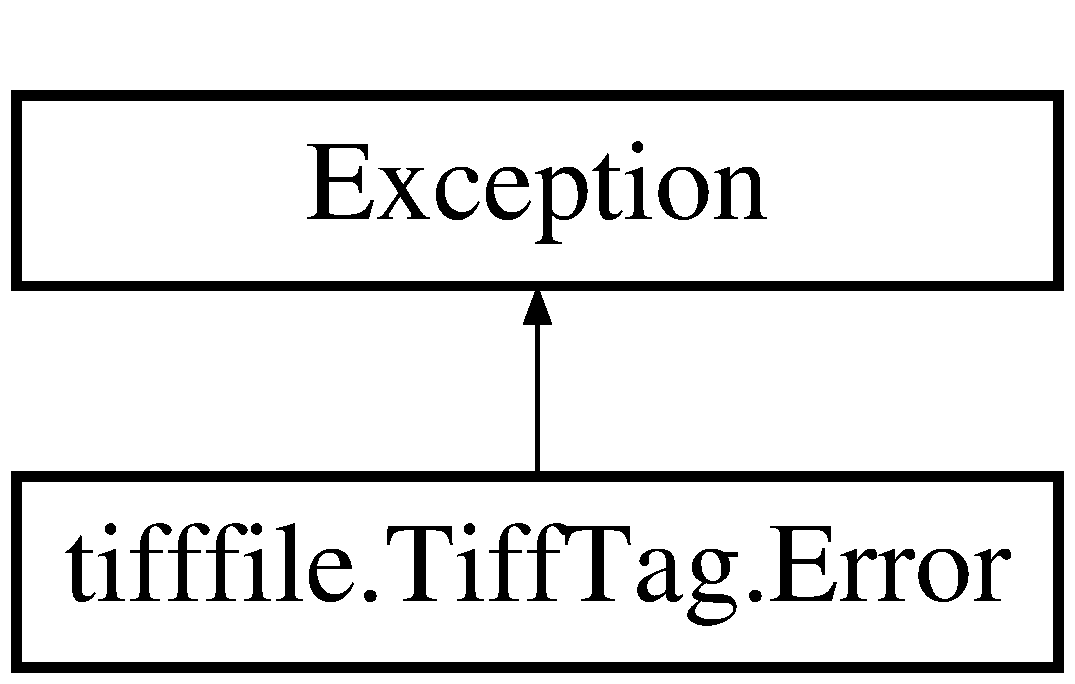
\includegraphics[height=2.000000cm]{classtifffile_1_1_tiff_tag_1_1_error}
\end{center}
\end{figure}


The documentation for this class was generated from the following file\-:\begin{DoxyCompactItemize}
\item 
workdir/atrex/\-Software/\hyperlink{tifffile_8py}{tifffile.\-py}\end{DoxyCompactItemize}

\hypertarget{classtifffile_1_1_file_handle}{\section{tifffile.\-File\-Handle Class Reference}
\label{classtifffile_1_1_file_handle}\index{tifffile.\-File\-Handle@{tifffile.\-File\-Handle}}
}
Inheritance diagram for tifffile.\-File\-Handle\-:\begin{figure}[H]
\begin{center}
\leavevmode
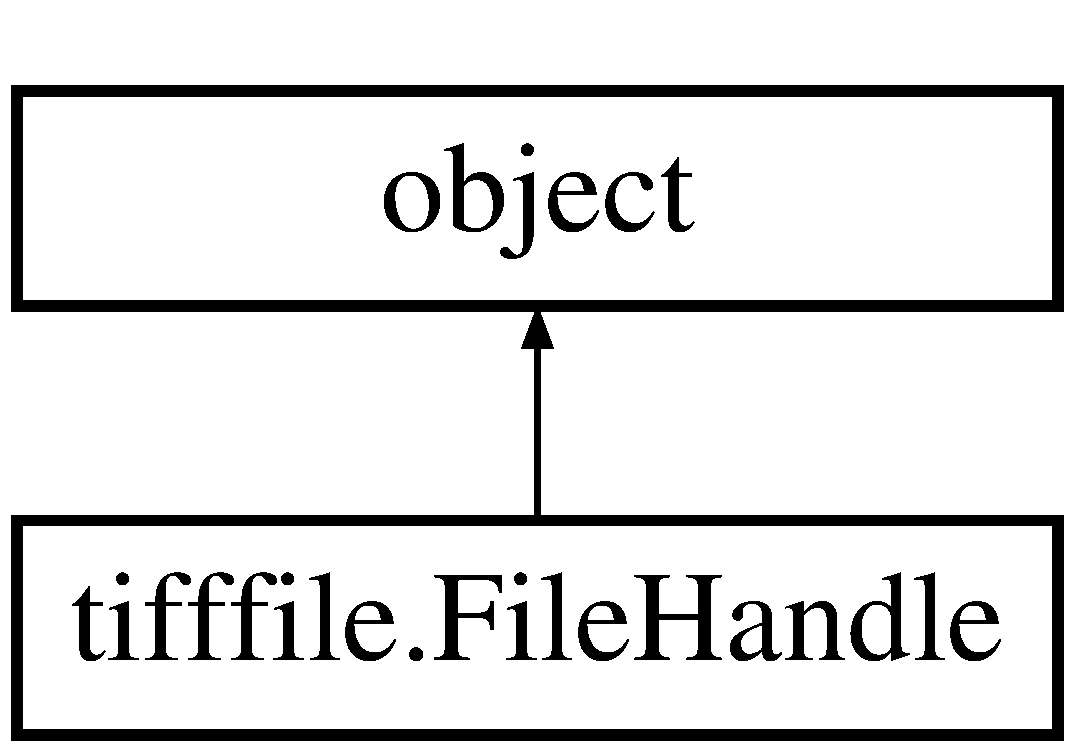
\includegraphics[height=2.000000cm]{classtifffile_1_1_file_handle}
\end{center}
\end{figure}
\subsection*{Public Member Functions}
\begin{DoxyCompactItemize}
\item 
def \hyperlink{classtifffile_1_1_file_handle_a256d28d56fa26bdc5a54056626dba06b}{\-\_\-\-\_\-init\-\_\-\-\_\-}
\item 
def \hyperlink{classtifffile_1_1_file_handle_aed5fb2120f32ee43f63a74e51ee19014}{open}
\item 
def \hyperlink{classtifffile_1_1_file_handle_a11284915485b77b0666fab6c13ff3052}{read}
\item 
def \hyperlink{classtifffile_1_1_file_handle_a57407ec5af06d23c9bad8c8b94a4c1e4}{memmap\-\_\-array}
\item 
def \hyperlink{classtifffile_1_1_file_handle_ae9a3b8d51a50d9cac82f80a33e3c9887}{read\-\_\-array}
\item 
def \hyperlink{classtifffile_1_1_file_handle_ace4a33bbf8c889940fea17f043042ce3}{read\-\_\-record}
\item 
def \hyperlink{classtifffile_1_1_file_handle_ac6a2ba4f361ef961cb206c2199513c70}{tell}
\item 
def \hyperlink{classtifffile_1_1_file_handle_a88d4b64db22c7a55afae0428b5e0200a}{seek}
\item 
def \hyperlink{classtifffile_1_1_file_handle_a8c345933b2368352aa97ee72aaeda596}{close}
\item 
def \hyperlink{classtifffile_1_1_file_handle_af0dcfc3f144e9ab96946cf8063142574}{\-\_\-\-\_\-enter\-\_\-\-\_\-}
\item 
def \hyperlink{classtifffile_1_1_file_handle_a7a59eb04f16fee7fafead1200bb4871b}{\-\_\-\-\_\-exit\-\_\-\-\_\-}
\item 
def \hyperlink{classtifffile_1_1_file_handle_a4ab2bf69b0a273e2ee43db2d9f2536b5}{\-\_\-\-\_\-getattr\-\_\-\-\_\-}
\item 
def \hyperlink{classtifffile_1_1_file_handle_a65426db83982602cb1e3e301eddf9fd6}{name}
\item 
def \hyperlink{classtifffile_1_1_file_handle_a1816f4d0d7568ebb37e4b473e527e106}{dirname}
\item 
def \hyperlink{classtifffile_1_1_file_handle_a23b95cb72e478e26496e6d3d7527a3a3}{path}
\item 
def \hyperlink{classtifffile_1_1_file_handle_a8fc096aaf40c918ccfc6f61304c63384}{size}
\item 
def \hyperlink{classtifffile_1_1_file_handle_ac35c2f69232e3c539f7b5859db1239c4}{closed}
\end{DoxyCompactItemize}
\subsection*{Public Attributes}
\begin{DoxyCompactItemize}
\item 
\hyperlink{classtifffile_1_1_file_handle_a965cb7fae14d9f259b2197072da2cf2e}{is\-\_\-file}
\end{DoxyCompactItemize}


\subsection{Detailed Description}
\begin{DoxyVerb}Binary file handle.

* Handle embedded files (for CZI within CZI files).
* Allow to re-open closed files (for multi file formats such as OME-TIFF).
* Read numpy arrays and records from file like objects.

Only binary read, seek, tell, and close are supported on embedded files.
When initialized from another file handle, do not use it unless this
FileHandle is closed.

Attributes
----------
name : str
    Name of the file.
path : str
    Absolute path to file.
size : int
    Size of file in bytes.
is_file : bool
    If True, file has a filno and can be memory mapped.

All attributes are read-only.\end{DoxyVerb}
 

\subsection{Constructor \& Destructor Documentation}
\hypertarget{classtifffile_1_1_file_handle_a256d28d56fa26bdc5a54056626dba06b}{\index{tifffile\-::\-File\-Handle@{tifffile\-::\-File\-Handle}!\-\_\-\-\_\-init\-\_\-\-\_\-@{\-\_\-\-\_\-init\-\_\-\-\_\-}}
\index{\-\_\-\-\_\-init\-\_\-\-\_\-@{\-\_\-\-\_\-init\-\_\-\-\_\-}!tifffile::FileHandle@{tifffile\-::\-File\-Handle}}
\subsubsection[{\-\_\-\-\_\-init\-\_\-\-\_\-}]{\setlength{\rightskip}{0pt plus 5cm}def tifffile.\-File\-Handle.\-\_\-\-\_\-init\-\_\-\-\_\- (
\begin{DoxyParamCaption}
\item[{}]{self, }
\item[{}]{arg, }
\item[{}]{mode = {\ttfamily 'rb'}, }
\item[{}]{name = {\ttfamily None}, }
\item[{}]{offset = {\ttfamily None}, }
\item[{}]{size = {\ttfamily None}}
\end{DoxyParamCaption}
)}}\label{classtifffile_1_1_file_handle_a256d28d56fa26bdc5a54056626dba06b}
\begin{DoxyVerb}Initialize file handle from file name or another file handle.

Parameters
----------
arg : str, File, or FileHandle
    File name or open file handle.
mode : str
    File open mode in case 'arg' is a file name.
name : str
    Optional name of file in case 'arg' is a file handle.
offset : int
    Optional start position of embedded file. By default this is
    the current file position.
size : int
    Optional size of embedded file. By default this is the number
    of bytes from the 'offset' to the end of the file.\end{DoxyVerb}
 

\subsection{Member Function Documentation}
\hypertarget{classtifffile_1_1_file_handle_af0dcfc3f144e9ab96946cf8063142574}{\index{tifffile\-::\-File\-Handle@{tifffile\-::\-File\-Handle}!\-\_\-\-\_\-enter\-\_\-\-\_\-@{\-\_\-\-\_\-enter\-\_\-\-\_\-}}
\index{\-\_\-\-\_\-enter\-\_\-\-\_\-@{\-\_\-\-\_\-enter\-\_\-\-\_\-}!tifffile::FileHandle@{tifffile\-::\-File\-Handle}}
\subsubsection[{\-\_\-\-\_\-enter\-\_\-\-\_\-}]{\setlength{\rightskip}{0pt plus 5cm}def tifffile.\-File\-Handle.\-\_\-\-\_\-enter\-\_\-\-\_\- (
\begin{DoxyParamCaption}
\item[{}]{self}
\end{DoxyParamCaption}
)}}\label{classtifffile_1_1_file_handle_af0dcfc3f144e9ab96946cf8063142574}
\hypertarget{classtifffile_1_1_file_handle_a7a59eb04f16fee7fafead1200bb4871b}{\index{tifffile\-::\-File\-Handle@{tifffile\-::\-File\-Handle}!\-\_\-\-\_\-exit\-\_\-\-\_\-@{\-\_\-\-\_\-exit\-\_\-\-\_\-}}
\index{\-\_\-\-\_\-exit\-\_\-\-\_\-@{\-\_\-\-\_\-exit\-\_\-\-\_\-}!tifffile::FileHandle@{tifffile\-::\-File\-Handle}}
\subsubsection[{\-\_\-\-\_\-exit\-\_\-\-\_\-}]{\setlength{\rightskip}{0pt plus 5cm}def tifffile.\-File\-Handle.\-\_\-\-\_\-exit\-\_\-\-\_\- (
\begin{DoxyParamCaption}
\item[{}]{self, }
\item[{}]{exc\-\_\-type, }
\item[{}]{exc\-\_\-value, }
\item[{}]{traceback}
\end{DoxyParamCaption}
)}}\label{classtifffile_1_1_file_handle_a7a59eb04f16fee7fafead1200bb4871b}
\hypertarget{classtifffile_1_1_file_handle_a4ab2bf69b0a273e2ee43db2d9f2536b5}{\index{tifffile\-::\-File\-Handle@{tifffile\-::\-File\-Handle}!\-\_\-\-\_\-getattr\-\_\-\-\_\-@{\-\_\-\-\_\-getattr\-\_\-\-\_\-}}
\index{\-\_\-\-\_\-getattr\-\_\-\-\_\-@{\-\_\-\-\_\-getattr\-\_\-\-\_\-}!tifffile::FileHandle@{tifffile\-::\-File\-Handle}}
\subsubsection[{\-\_\-\-\_\-getattr\-\_\-\-\_\-}]{\setlength{\rightskip}{0pt plus 5cm}def tifffile.\-File\-Handle.\-\_\-\-\_\-getattr\-\_\-\-\_\- (
\begin{DoxyParamCaption}
\item[{}]{self, }
\item[{}]{name}
\end{DoxyParamCaption}
)}}\label{classtifffile_1_1_file_handle_a4ab2bf69b0a273e2ee43db2d9f2536b5}
\begin{DoxyVerb}Return attribute from underlying file object.\end{DoxyVerb}
 \hypertarget{classtifffile_1_1_file_handle_a8c345933b2368352aa97ee72aaeda596}{\index{tifffile\-::\-File\-Handle@{tifffile\-::\-File\-Handle}!close@{close}}
\index{close@{close}!tifffile::FileHandle@{tifffile\-::\-File\-Handle}}
\subsubsection[{close}]{\setlength{\rightskip}{0pt plus 5cm}def tifffile.\-File\-Handle.\-close (
\begin{DoxyParamCaption}
\item[{}]{self}
\end{DoxyParamCaption}
)}}\label{classtifffile_1_1_file_handle_a8c345933b2368352aa97ee72aaeda596}
\begin{DoxyVerb}Close file.\end{DoxyVerb}
 \hypertarget{classtifffile_1_1_file_handle_ac35c2f69232e3c539f7b5859db1239c4}{\index{tifffile\-::\-File\-Handle@{tifffile\-::\-File\-Handle}!closed@{closed}}
\index{closed@{closed}!tifffile::FileHandle@{tifffile\-::\-File\-Handle}}
\subsubsection[{closed}]{\setlength{\rightskip}{0pt plus 5cm}def tifffile.\-File\-Handle.\-closed (
\begin{DoxyParamCaption}
\item[{}]{self}
\end{DoxyParamCaption}
)}}\label{classtifffile_1_1_file_handle_ac35c2f69232e3c539f7b5859db1239c4}
\hypertarget{classtifffile_1_1_file_handle_a1816f4d0d7568ebb37e4b473e527e106}{\index{tifffile\-::\-File\-Handle@{tifffile\-::\-File\-Handle}!dirname@{dirname}}
\index{dirname@{dirname}!tifffile::FileHandle@{tifffile\-::\-File\-Handle}}
\subsubsection[{dirname}]{\setlength{\rightskip}{0pt plus 5cm}def tifffile.\-File\-Handle.\-dirname (
\begin{DoxyParamCaption}
\item[{}]{self}
\end{DoxyParamCaption}
)}}\label{classtifffile_1_1_file_handle_a1816f4d0d7568ebb37e4b473e527e106}
\hypertarget{classtifffile_1_1_file_handle_a57407ec5af06d23c9bad8c8b94a4c1e4}{\index{tifffile\-::\-File\-Handle@{tifffile\-::\-File\-Handle}!memmap\-\_\-array@{memmap\-\_\-array}}
\index{memmap\-\_\-array@{memmap\-\_\-array}!tifffile::FileHandle@{tifffile\-::\-File\-Handle}}
\subsubsection[{memmap\-\_\-array}]{\setlength{\rightskip}{0pt plus 5cm}def tifffile.\-File\-Handle.\-memmap\-\_\-array (
\begin{DoxyParamCaption}
\item[{}]{self, }
\item[{}]{dtype, }
\item[{}]{shape, }
\item[{}]{offset = {\ttfamily 0}, }
\item[{}]{mode = {\ttfamily 'r'}, }
\item[{}]{order = {\ttfamily 'C'}}
\end{DoxyParamCaption}
)}}\label{classtifffile_1_1_file_handle_a57407ec5af06d23c9bad8c8b94a4c1e4}
\begin{DoxyVerb}Return numpy.memmap of data stored in file.\end{DoxyVerb}
 \hypertarget{classtifffile_1_1_file_handle_a65426db83982602cb1e3e301eddf9fd6}{\index{tifffile\-::\-File\-Handle@{tifffile\-::\-File\-Handle}!name@{name}}
\index{name@{name}!tifffile::FileHandle@{tifffile\-::\-File\-Handle}}
\subsubsection[{name}]{\setlength{\rightskip}{0pt plus 5cm}def tifffile.\-File\-Handle.\-name (
\begin{DoxyParamCaption}
\item[{}]{self}
\end{DoxyParamCaption}
)}}\label{classtifffile_1_1_file_handle_a65426db83982602cb1e3e301eddf9fd6}
\hypertarget{classtifffile_1_1_file_handle_aed5fb2120f32ee43f63a74e51ee19014}{\index{tifffile\-::\-File\-Handle@{tifffile\-::\-File\-Handle}!open@{open}}
\index{open@{open}!tifffile::FileHandle@{tifffile\-::\-File\-Handle}}
\subsubsection[{open}]{\setlength{\rightskip}{0pt plus 5cm}def tifffile.\-File\-Handle.\-open (
\begin{DoxyParamCaption}
\item[{}]{self}
\end{DoxyParamCaption}
)}}\label{classtifffile_1_1_file_handle_aed5fb2120f32ee43f63a74e51ee19014}
\begin{DoxyVerb}Open or re-open file.\end{DoxyVerb}
 \hypertarget{classtifffile_1_1_file_handle_a23b95cb72e478e26496e6d3d7527a3a3}{\index{tifffile\-::\-File\-Handle@{tifffile\-::\-File\-Handle}!path@{path}}
\index{path@{path}!tifffile::FileHandle@{tifffile\-::\-File\-Handle}}
\subsubsection[{path}]{\setlength{\rightskip}{0pt plus 5cm}def tifffile.\-File\-Handle.\-path (
\begin{DoxyParamCaption}
\item[{}]{self}
\end{DoxyParamCaption}
)}}\label{classtifffile_1_1_file_handle_a23b95cb72e478e26496e6d3d7527a3a3}
\hypertarget{classtifffile_1_1_file_handle_a11284915485b77b0666fab6c13ff3052}{\index{tifffile\-::\-File\-Handle@{tifffile\-::\-File\-Handle}!read@{read}}
\index{read@{read}!tifffile::FileHandle@{tifffile\-::\-File\-Handle}}
\subsubsection[{read}]{\setlength{\rightskip}{0pt plus 5cm}def tifffile.\-File\-Handle.\-read (
\begin{DoxyParamCaption}
\item[{}]{self, }
\item[{}]{size = {\ttfamily -\/1}}
\end{DoxyParamCaption}
)}}\label{classtifffile_1_1_file_handle_a11284915485b77b0666fab6c13ff3052}
\begin{DoxyVerb}Read 'size' bytes from file, or until EOF is reached.\end{DoxyVerb}
 \hypertarget{classtifffile_1_1_file_handle_ae9a3b8d51a50d9cac82f80a33e3c9887}{\index{tifffile\-::\-File\-Handle@{tifffile\-::\-File\-Handle}!read\-\_\-array@{read\-\_\-array}}
\index{read\-\_\-array@{read\-\_\-array}!tifffile::FileHandle@{tifffile\-::\-File\-Handle}}
\subsubsection[{read\-\_\-array}]{\setlength{\rightskip}{0pt plus 5cm}def tifffile.\-File\-Handle.\-read\-\_\-array (
\begin{DoxyParamCaption}
\item[{}]{self, }
\item[{}]{dtype, }
\item[{}]{count = {\ttfamily -\/1}, }
\item[{}]{sep = {\ttfamily \char`\"{}\char`\"{}}}
\end{DoxyParamCaption}
)}}\label{classtifffile_1_1_file_handle_ae9a3b8d51a50d9cac82f80a33e3c9887}
\begin{DoxyVerb}Return numpy array from file.

Work around numpy issue #2230, "numpy.fromfile does not accept
StringIO object" https://github.com/numpy/numpy/issues/2230.\end{DoxyVerb}
 \hypertarget{classtifffile_1_1_file_handle_ace4a33bbf8c889940fea17f043042ce3}{\index{tifffile\-::\-File\-Handle@{tifffile\-::\-File\-Handle}!read\-\_\-record@{read\-\_\-record}}
\index{read\-\_\-record@{read\-\_\-record}!tifffile::FileHandle@{tifffile\-::\-File\-Handle}}
\subsubsection[{read\-\_\-record}]{\setlength{\rightskip}{0pt plus 5cm}def tifffile.\-File\-Handle.\-read\-\_\-record (
\begin{DoxyParamCaption}
\item[{}]{self, }
\item[{}]{dtype, }
\item[{}]{shape = {\ttfamily 1}, }
\item[{}]{byteorder = {\ttfamily None}}
\end{DoxyParamCaption}
)}}\label{classtifffile_1_1_file_handle_ace4a33bbf8c889940fea17f043042ce3}
\begin{DoxyVerb}Return numpy record from file.\end{DoxyVerb}
 \hypertarget{classtifffile_1_1_file_handle_a88d4b64db22c7a55afae0428b5e0200a}{\index{tifffile\-::\-File\-Handle@{tifffile\-::\-File\-Handle}!seek@{seek}}
\index{seek@{seek}!tifffile::FileHandle@{tifffile\-::\-File\-Handle}}
\subsubsection[{seek}]{\setlength{\rightskip}{0pt plus 5cm}def tifffile.\-File\-Handle.\-seek (
\begin{DoxyParamCaption}
\item[{}]{self, }
\item[{}]{offset, }
\item[{}]{whence = {\ttfamily 0}}
\end{DoxyParamCaption}
)}}\label{classtifffile_1_1_file_handle_a88d4b64db22c7a55afae0428b5e0200a}
\begin{DoxyVerb}Set file's current position.\end{DoxyVerb}
 \hypertarget{classtifffile_1_1_file_handle_a8fc096aaf40c918ccfc6f61304c63384}{\index{tifffile\-::\-File\-Handle@{tifffile\-::\-File\-Handle}!size@{size}}
\index{size@{size}!tifffile::FileHandle@{tifffile\-::\-File\-Handle}}
\subsubsection[{size}]{\setlength{\rightskip}{0pt plus 5cm}def tifffile.\-File\-Handle.\-size (
\begin{DoxyParamCaption}
\item[{}]{self}
\end{DoxyParamCaption}
)}}\label{classtifffile_1_1_file_handle_a8fc096aaf40c918ccfc6f61304c63384}
\hypertarget{classtifffile_1_1_file_handle_ac6a2ba4f361ef961cb206c2199513c70}{\index{tifffile\-::\-File\-Handle@{tifffile\-::\-File\-Handle}!tell@{tell}}
\index{tell@{tell}!tifffile::FileHandle@{tifffile\-::\-File\-Handle}}
\subsubsection[{tell}]{\setlength{\rightskip}{0pt plus 5cm}def tifffile.\-File\-Handle.\-tell (
\begin{DoxyParamCaption}
\item[{}]{self}
\end{DoxyParamCaption}
)}}\label{classtifffile_1_1_file_handle_ac6a2ba4f361ef961cb206c2199513c70}
\begin{DoxyVerb}Return file's current position.\end{DoxyVerb}
 

\subsection{Member Data Documentation}
\hypertarget{classtifffile_1_1_file_handle_a965cb7fae14d9f259b2197072da2cf2e}{\index{tifffile\-::\-File\-Handle@{tifffile\-::\-File\-Handle}!is\-\_\-file@{is\-\_\-file}}
\index{is\-\_\-file@{is\-\_\-file}!tifffile::FileHandle@{tifffile\-::\-File\-Handle}}
\subsubsection[{is\-\_\-file}]{\setlength{\rightskip}{0pt plus 5cm}tifffile.\-File\-Handle.\-is\-\_\-file}}\label{classtifffile_1_1_file_handle_a965cb7fae14d9f259b2197072da2cf2e}


The documentation for this class was generated from the following file\-:\begin{DoxyCompactItemize}
\item 
workdir/atrex/\-Software/\hyperlink{tifffile_8py}{tifffile.\-py}\end{DoxyCompactItemize}

\hypertarget{class_j_c_p_d_s_1_1_j_c_p_d_s}{\section{J\-C\-P\-D\-S.\-J\-C\-P\-D\-S Class Reference}
\label{class_j_c_p_d_s_1_1_j_c_p_d_s}\index{J\-C\-P\-D\-S.\-J\-C\-P\-D\-S@{J\-C\-P\-D\-S.\-J\-C\-P\-D\-S}}
}
\subsection*{Public Member Functions}
\begin{DoxyCompactItemize}
\item 
def \hyperlink{class_j_c_p_d_s_1_1_j_c_p_d_s_aca0207da67855730a22a3bbcd031c1d3}{\-\_\-\-\_\-init\-\_\-\-\_\-}
\item 
def \hyperlink{class_j_c_p_d_s_1_1_j_c_p_d_s_ab3335931a8dbbff1bff32de39d752723}{read\-\_\-file}
\item 
def \hyperlink{class_j_c_p_d_s_1_1_j_c_p_d_s_a728290518d30c0c2df73cf1383515768}{read\-\_\-xpow}
\item 
def \hyperlink{class_j_c_p_d_s_1_1_j_c_p_d_s_a229ed071c04b6cb367ea7b349539e711}{write\-\_\-file}
\item 
def \hyperlink{class_j_c_p_d_s_1_1_j_c_p_d_s_a9bce7cbc5045239ca4175d750256e6aa}{compute\-\_\-\-D}
\item 
def \hyperlink{class_j_c_p_d_s_1_1_j_c_p_d_s_a3d9ee706776a7e24826e8a21ac8ac51a}{compute\-\_\-v0}
\item 
def \hyperlink{class_j_c_p_d_s_1_1_j_c_p_d_s_a15973313ee7187e0e0bef03b1aebed0e}{compute\-\_\-v}
\item 
def \hyperlink{class_j_c_p_d_s_1_1_j_c_p_d_s_aa837bef35e9c46e89a6c2673dfaa10b8}{compute\-\_\-volume}
\item 
def \hyperlink{class_j_c_p_d_s_1_1_j_c_p_d_s_ad256df2c1ea42c6ed31ff86bb577981a}{bm3\-\_\-pressure}
\item 
def \hyperlink{class_j_c_p_d_s_1_1_j_c_p_d_s_a73e3fb2c332bde54412906eaf49b5693}{check\-\_\-for\-\_\-equivalents}
\item 
def \hyperlink{class_j_c_p_d_s_1_1_j_c_p_d_s_acd0737c833865f0efd2b3e8dd273c909}{copy\-\_\-object1}
\item 
def \hyperlink{class_j_c_p_d_s_1_1_j_c_p_d_s_a3ce0c985ae5d2016ace2766ca2f520ee}{copy\-\_\-object}
\item 
def \hyperlink{class_j_c_p_d_s_1_1_j_c_p_d_s_aa3b28978840f14b05fa13d88d083b214}{generate\-\_\-accessible\-\_\-peaks}
\item 
def \hyperlink{class_j_c_p_d_s_1_1_j_c_p_d_s_a32a90e34a4d32069f00a6f6537dc91dc}{get\-\_\-ks}
\item 
def \hyperlink{class_j_c_p_d_s_1_1_j_c_p_d_s_a36e77efd2364a3f81ef463ffb959d07e}{set\-\_\-ks}
\item 
def \hyperlink{class_j_c_p_d_s_1_1_j_c_p_d_s_a06b183ba8881c7197a063b860083dfd8}{get\-\_\-lp}
\item 
def \hyperlink{class_j_c_p_d_s_1_1_j_c_p_d_s_aabe3f59ba92dfb4712082c77d74a28b0}{get\-\_\-lp0}
\item 
def \hyperlink{class_j_c_p_d_s_1_1_j_c_p_d_s_a957b63b325687580b686ea88741fdfb8}{calculate\-\_\-abc}
\item 
def \hyperlink{class_j_c_p_d_s_1_1_j_c_p_d_s_aaf4441ec7e191848281e381982568c74}{set\-\_\-lp}
\item 
def \hyperlink{class_j_c_p_d_s_1_1_j_c_p_d_s_abe8101e5474e729f2d067fcc61561a31}{set\-\_\-lp0}
\item 
def \hyperlink{class_j_c_p_d_s_1_1_j_c_p_d_s_a92e518955551c7e65dad79bb40d5181a}{get\-\_\-symmetry}
\item 
def \hyperlink{class_j_c_p_d_s_1_1_j_c_p_d_s_a8cd753161864e176f79874f9ee55ca9b}{set\-\_\-symmetry}
\item 
def \hyperlink{class_j_c_p_d_s_1_1_j_c_p_d_s_ab2c9774755de8f1b98fbd75fca00281e}{set\-\_\-comment}
\item 
def \hyperlink{class_j_c_p_d_s_1_1_j_c_p_d_s_ab93dd1b1d99684d5ee51713afc042413}{get\-\_\-comment}
\item 
def \hyperlink{class_j_c_p_d_s_1_1_j_c_p_d_s_adf2e6b325f00594a550653a6a150215d}{set\-\_\-reflections}
\item 
def \hyperlink{class_j_c_p_d_s_1_1_j_c_p_d_s_a125df1699b3e7f91e14e19c7035152e9}{get\-\_\-reflections\-\_\-\-P\-C}
\item 
def \hyperlink{class_j_c_p_d_s_1_1_j_c_p_d_s_a1d48c932a6349263167926e057807c3f}{get\-Param\-String}
\end{DoxyCompactItemize}
\subsection*{Public Attributes}
\begin{DoxyCompactItemize}
\item 
\hyperlink{class_j_c_p_d_s_1_1_j_c_p_d_s_a809397a9da7c35ae0a3ad9fca1cabc73}{a}
\item 
\hyperlink{class_j_c_p_d_s_1_1_j_c_p_d_s_af32006e867dad5c863a396af1590c34f}{version}
\item 
\hyperlink{class_j_c_p_d_s_1_1_j_c_p_d_s_ac7bb249be2c2ff3d89ca89c5cf9fba26}{filename}
\item 
\hyperlink{class_j_c_p_d_s_1_1_j_c_p_d_s_a5107a25f1f6940a39ce5f7391ff87b21}{k0}
\item 
\hyperlink{class_j_c_p_d_s_1_1_j_c_p_d_s_a20801fc810dd360855e81c7c8c486d78}{k0p}
\item 
\hyperlink{class_j_c_p_d_s_1_1_j_c_p_d_s_a1423572b84a46fa0739fba9892d55fdf}{dk0dt}
\item 
\hyperlink{class_j_c_p_d_s_1_1_j_c_p_d_s_a281da0716f471977727858228cbddaa4}{dk0pdt}
\item 
\hyperlink{class_j_c_p_d_s_1_1_j_c_p_d_s_af8dfc3bb57b6bd48b9eeed7d4eb19685}{symmetry}
\item 
\hyperlink{class_j_c_p_d_s_1_1_j_c_p_d_s_acfb0a8fef740164e10c7b87d92aa82d6}{a0}
\item 
\hyperlink{class_j_c_p_d_s_1_1_j_c_p_d_s_a7760bcfe96b190ba393928e70ed996cb}{b0}
\item 
\hyperlink{class_j_c_p_d_s_1_1_j_c_p_d_s_a81fa032e6345e4ec9baa962f65507ef6}{c0}
\item 
\hyperlink{class_j_c_p_d_s_1_1_j_c_p_d_s_a8b17a58f7870b085673c881db21b8335}{alpha0}
\item 
\hyperlink{class_j_c_p_d_s_1_1_j_c_p_d_s_a45086584379c67ece36240b890741c61}{beta0}
\item 
\hyperlink{class_j_c_p_d_s_1_1_j_c_p_d_s_aa9826897893cdc97c509c90187c61d8c}{gamma0}
\item 
\hyperlink{class_j_c_p_d_s_1_1_j_c_p_d_s_aef3a4e5b9b3659dc953d276e53a12743}{v0}
\item 
\hyperlink{class_j_c_p_d_s_1_1_j_c_p_d_s_ae09f3ff37073046c2ceb1c1aa3a6864c}{alphat}
\item 
\hyperlink{class_j_c_p_d_s_1_1_j_c_p_d_s_a1254951d6b1ef48336305b1ad1175394}{dalphadt}
\item 
\hyperlink{class_j_c_p_d_s_1_1_j_c_p_d_s_a676bd92e3b0d5b98eccc73b3caf63adf}{b}
\item 
\hyperlink{class_j_c_p_d_s_1_1_j_c_p_d_s_ac9317030388422ba002d811107a89a6b}{c}
\item 
\hyperlink{class_j_c_p_d_s_1_1_j_c_p_d_s_af6fdcb71ae44429648d063792c60fdfd}{d}
\item 
\hyperlink{class_j_c_p_d_s_1_1_j_c_p_d_s_ac75745e6c3de323e88814c7175a9d60c}{alpha}
\item 
\hyperlink{class_j_c_p_d_s_1_1_j_c_p_d_s_a124176c2b50872c9722c7cadb745916b}{beta}
\item 
\hyperlink{class_j_c_p_d_s_1_1_j_c_p_d_s_a979816f1d0a94fb06cc9f764d9d51b0f}{gamma}
\item 
\hyperlink{class_j_c_p_d_s_1_1_j_c_p_d_s_a7bb271b77b0a3dacfb0fbf27bced86a2}{v}
\item 
\hyperlink{class_j_c_p_d_s_1_1_j_c_p_d_s_a938f17d1d1d0e167248e24c127f52c1c}{reflections}
\item 
\hyperlink{class_j_c_p_d_s_1_1_j_c_p_d_s_ae1ed69e9ad7a3dbc9fa8f1a4e9fdc5c8}{comment}
\end{DoxyCompactItemize}
\subsection*{Static Public Attributes}
\begin{DoxyCompactItemize}
\item 
int \hyperlink{class_j_c_p_d_s_1_1_j_c_p_d_s_a9418ae33987e25bb6cff0c2de64f8b60}{a} = 0
\item 
int \hyperlink{class_j_c_p_d_s_1_1_j_c_p_d_s_a0a05ddd20692ac7885c02090c80ae9b2}{b} = 0
\item 
int \hyperlink{class_j_c_p_d_s_1_1_j_c_p_d_s_a48449d973d4dba83f73cf5da725a9616}{c} = 0
\item 
int \hyperlink{class_j_c_p_d_s_1_1_j_c_p_d_s_a73e6b491c6ebf61ea16474472b57f1fd}{d} = 0
\item 
int \hyperlink{class_j_c_p_d_s_1_1_j_c_p_d_s_aaa0b2a4a0b3ca6a97ea2fc55c905c29f}{a0} = 0
\item 
int \hyperlink{class_j_c_p_d_s_1_1_j_c_p_d_s_af88aaff23be0026b70e55f09a6e73acb}{b0} = 0
\item 
int \hyperlink{class_j_c_p_d_s_1_1_j_c_p_d_s_aba1a3a8c603a94e0b3ed6babbfd09734}{c0} = 0
\item 
int \hyperlink{class_j_c_p_d_s_1_1_j_c_p_d_s_acc2fd1c621c0be8f860827f3006157ee}{d0} = 0
\item 
list \hyperlink{class_j_c_p_d_s_1_1_j_c_p_d_s_a0baef80c76433cded445041b5d0e29d5}{comment} = \mbox{[}$\,$\mbox{]}
\item 
list \hyperlink{class_j_c_p_d_s_1_1_j_c_p_d_s_a4a667612a80191cc64ec7d06c27f4f84}{reflections} = \mbox{[}$\,$\mbox{]}
\item 
string \hyperlink{class_j_c_p_d_s_1_1_j_c_p_d_s_afde1c6e0f66289f1431e29b25df8a6b4}{symmetry} = 'C\-U\-B\-I\-C'
\item 
string \hyperlink{class_j_c_p_d_s_1_1_j_c_p_d_s_a24c99728583d07ecfc59ea617634a333}{filename} = ''
\item 
string \hyperlink{class_j_c_p_d_s_1_1_j_c_p_d_s_a48e76018a03f8c6fd3a7b3dfbccaf0f7}{file} = ''
\item 
int \hyperlink{class_j_c_p_d_s_1_1_j_c_p_d_s_a16bc3288893c02b04d91bd8a3fa315fe}{version} = 0
\item 
int \hyperlink{class_j_c_p_d_s_1_1_j_c_p_d_s_a669f40a36a77a7dab00da06bb5c2ec92}{k0} = 0
\item 
int \hyperlink{class_j_c_p_d_s_1_1_j_c_p_d_s_ac42204eb0a9727b57b1b0957937d60d0}{k0p} = 0
\item 
int \hyperlink{class_j_c_p_d_s_1_1_j_c_p_d_s_a3c24a9159dff627119de99dcdb4379b0}{dk0dt} = 0
\item 
int \hyperlink{class_j_c_p_d_s_1_1_j_c_p_d_s_a4366bab3d24002031f7c7ab9b19af05f}{dk0pdt} = 0
\item 
int \hyperlink{class_j_c_p_d_s_1_1_j_c_p_d_s_a99ef62d67765d544bc2c92f0e57155fa}{alphat} = 0
\item 
int \hyperlink{class_j_c_p_d_s_1_1_j_c_p_d_s_abbefe291cd0b1042d2e999030e621bb8}{dalphadt} = 0
\item 
int \hyperlink{class_j_c_p_d_s_1_1_j_c_p_d_s_a93c4313c55cb15fef00bf85ef6a5e1c3}{alpha0} = 0
\item 
int \hyperlink{class_j_c_p_d_s_1_1_j_c_p_d_s_a28cdaa7d634aa5683e2b9b3f5f0d32e7}{beta0} = 0
\item 
int \hyperlink{class_j_c_p_d_s_1_1_j_c_p_d_s_a64bff5a1dafc26de47247bd07b858774}{gamma0} = 0
\item 
int \hyperlink{class_j_c_p_d_s_1_1_j_c_p_d_s_af4550ef102f3c38e2da9fe2e29b2c95b}{alpha} = 0
\item 
int \hyperlink{class_j_c_p_d_s_1_1_j_c_p_d_s_aa5dde75830b82228fb5424b31f1d5ec2}{beta} = 0
\item 
int \hyperlink{class_j_c_p_d_s_1_1_j_c_p_d_s_a5400cdc3eb14af0cf773e9bc83a9817c}{gamma} = 0
\item 
int \hyperlink{class_j_c_p_d_s_1_1_j_c_p_d_s_aaef6e23360b1e68d8cfdcad1c60fb88f}{v0} = 0
\item 
int \hyperlink{class_j_c_p_d_s_1_1_j_c_p_d_s_aba3d9f6fdf4c176b7263d5657b602aaa}{v} = 0
\end{DoxyCompactItemize}


\subsection{Constructor \& Destructor Documentation}
\hypertarget{class_j_c_p_d_s_1_1_j_c_p_d_s_aca0207da67855730a22a3bbcd031c1d3}{\index{J\-C\-P\-D\-S\-::\-J\-C\-P\-D\-S@{J\-C\-P\-D\-S\-::\-J\-C\-P\-D\-S}!\-\_\-\-\_\-init\-\_\-\-\_\-@{\-\_\-\-\_\-init\-\_\-\-\_\-}}
\index{\-\_\-\-\_\-init\-\_\-\-\_\-@{\-\_\-\-\_\-init\-\_\-\-\_\-}!JCPDS::JCPDS@{J\-C\-P\-D\-S\-::\-J\-C\-P\-D\-S}}
\subsubsection[{\-\_\-\-\_\-init\-\_\-\-\_\-}]{\setlength{\rightskip}{0pt plus 5cm}def J\-C\-P\-D\-S.\-J\-C\-P\-D\-S.\-\_\-\-\_\-init\-\_\-\-\_\- (
\begin{DoxyParamCaption}
\item[{}]{self}
\end{DoxyParamCaption}
)}}\label{class_j_c_p_d_s_1_1_j_c_p_d_s_aca0207da67855730a22a3bbcd031c1d3}


\subsection{Member Function Documentation}
\hypertarget{class_j_c_p_d_s_1_1_j_c_p_d_s_ad256df2c1ea42c6ed31ff86bb577981a}{\index{J\-C\-P\-D\-S\-::\-J\-C\-P\-D\-S@{J\-C\-P\-D\-S\-::\-J\-C\-P\-D\-S}!bm3\-\_\-pressure@{bm3\-\_\-pressure}}
\index{bm3\-\_\-pressure@{bm3\-\_\-pressure}!JCPDS::JCPDS@{J\-C\-P\-D\-S\-::\-J\-C\-P\-D\-S}}
\subsubsection[{bm3\-\_\-pressure}]{\setlength{\rightskip}{0pt plus 5cm}def J\-C\-P\-D\-S.\-J\-C\-P\-D\-S.\-bm3\-\_\-pressure (
\begin{DoxyParamCaption}
\item[{}]{self}
\end{DoxyParamCaption}
)}}\label{class_j_c_p_d_s_1_1_j_c_p_d_s_ad256df2c1ea42c6ed31ff86bb577981a}
\hypertarget{class_j_c_p_d_s_1_1_j_c_p_d_s_a957b63b325687580b686ea88741fdfb8}{\index{J\-C\-P\-D\-S\-::\-J\-C\-P\-D\-S@{J\-C\-P\-D\-S\-::\-J\-C\-P\-D\-S}!calculate\-\_\-abc@{calculate\-\_\-abc}}
\index{calculate\-\_\-abc@{calculate\-\_\-abc}!JCPDS::JCPDS@{J\-C\-P\-D\-S\-::\-J\-C\-P\-D\-S}}
\subsubsection[{calculate\-\_\-abc}]{\setlength{\rightskip}{0pt plus 5cm}def J\-C\-P\-D\-S.\-J\-C\-P\-D\-S.\-calculate\-\_\-abc (
\begin{DoxyParamCaption}
\item[{}]{self, }
\item[{}]{p, }
\item[{}]{T}
\end{DoxyParamCaption}
)}}\label{class_j_c_p_d_s_1_1_j_c_p_d_s_a957b63b325687580b686ea88741fdfb8}
\hypertarget{class_j_c_p_d_s_1_1_j_c_p_d_s_a73e3fb2c332bde54412906eaf49b5693}{\index{J\-C\-P\-D\-S\-::\-J\-C\-P\-D\-S@{J\-C\-P\-D\-S\-::\-J\-C\-P\-D\-S}!check\-\_\-for\-\_\-equivalents@{check\-\_\-for\-\_\-equivalents}}
\index{check\-\_\-for\-\_\-equivalents@{check\-\_\-for\-\_\-equivalents}!JCPDS::JCPDS@{J\-C\-P\-D\-S\-::\-J\-C\-P\-D\-S}}
\subsubsection[{check\-\_\-for\-\_\-equivalents}]{\setlength{\rightskip}{0pt plus 5cm}def J\-C\-P\-D\-S.\-J\-C\-P\-D\-S.\-check\-\_\-for\-\_\-equivalents (
\begin{DoxyParamCaption}
\item[{}]{self, }
\item[{}]{refs, }
\item[{}]{hkl, }
\item[{}]{N, }
\item[{}]{exti}
\end{DoxyParamCaption}
)}}\label{class_j_c_p_d_s_1_1_j_c_p_d_s_a73e3fb2c332bde54412906eaf49b5693}
\hypertarget{class_j_c_p_d_s_1_1_j_c_p_d_s_a9bce7cbc5045239ca4175d750256e6aa}{\index{J\-C\-P\-D\-S\-::\-J\-C\-P\-D\-S@{J\-C\-P\-D\-S\-::\-J\-C\-P\-D\-S}!compute\-\_\-\-D@{compute\-\_\-\-D}}
\index{compute\-\_\-\-D@{compute\-\_\-\-D}!JCPDS::JCPDS@{J\-C\-P\-D\-S\-::\-J\-C\-P\-D\-S}}
\subsubsection[{compute\-\_\-\-D}]{\setlength{\rightskip}{0pt plus 5cm}def J\-C\-P\-D\-S.\-J\-C\-P\-D\-S.\-compute\-\_\-\-D (
\begin{DoxyParamCaption}
\item[{}]{self, }
\item[{}]{Press = {\ttfamily 0}, }
\item[{}]{Temp = {\ttfamily 298}}
\end{DoxyParamCaption}
)}}\label{class_j_c_p_d_s_1_1_j_c_p_d_s_a9bce7cbc5045239ca4175d750256e6aa}
\hypertarget{class_j_c_p_d_s_1_1_j_c_p_d_s_a15973313ee7187e0e0bef03b1aebed0e}{\index{J\-C\-P\-D\-S\-::\-J\-C\-P\-D\-S@{J\-C\-P\-D\-S\-::\-J\-C\-P\-D\-S}!compute\-\_\-v@{compute\-\_\-v}}
\index{compute\-\_\-v@{compute\-\_\-v}!JCPDS::JCPDS@{J\-C\-P\-D\-S\-::\-J\-C\-P\-D\-S}}
\subsubsection[{compute\-\_\-v}]{\setlength{\rightskip}{0pt plus 5cm}def J\-C\-P\-D\-S.\-J\-C\-P\-D\-S.\-compute\-\_\-v (
\begin{DoxyParamCaption}
\item[{}]{self}
\end{DoxyParamCaption}
)}}\label{class_j_c_p_d_s_1_1_j_c_p_d_s_a15973313ee7187e0e0bef03b1aebed0e}
\hypertarget{class_j_c_p_d_s_1_1_j_c_p_d_s_a3d9ee706776a7e24826e8a21ac8ac51a}{\index{J\-C\-P\-D\-S\-::\-J\-C\-P\-D\-S@{J\-C\-P\-D\-S\-::\-J\-C\-P\-D\-S}!compute\-\_\-v0@{compute\-\_\-v0}}
\index{compute\-\_\-v0@{compute\-\_\-v0}!JCPDS::JCPDS@{J\-C\-P\-D\-S\-::\-J\-C\-P\-D\-S}}
\subsubsection[{compute\-\_\-v0}]{\setlength{\rightskip}{0pt plus 5cm}def J\-C\-P\-D\-S.\-J\-C\-P\-D\-S.\-compute\-\_\-v0 (
\begin{DoxyParamCaption}
\item[{}]{self}
\end{DoxyParamCaption}
)}}\label{class_j_c_p_d_s_1_1_j_c_p_d_s_a3d9ee706776a7e24826e8a21ac8ac51a}
\hypertarget{class_j_c_p_d_s_1_1_j_c_p_d_s_aa837bef35e9c46e89a6c2673dfaa10b8}{\index{J\-C\-P\-D\-S\-::\-J\-C\-P\-D\-S@{J\-C\-P\-D\-S\-::\-J\-C\-P\-D\-S}!compute\-\_\-volume@{compute\-\_\-volume}}
\index{compute\-\_\-volume@{compute\-\_\-volume}!JCPDS::JCPDS@{J\-C\-P\-D\-S\-::\-J\-C\-P\-D\-S}}
\subsubsection[{compute\-\_\-volume}]{\setlength{\rightskip}{0pt plus 5cm}def J\-C\-P\-D\-S.\-J\-C\-P\-D\-S.\-compute\-\_\-volume (
\begin{DoxyParamCaption}
\item[{}]{self, }
\item[{}]{pressure = {\ttfamily 0.}, }
\item[{}]{temp = {\ttfamily 298.}}
\end{DoxyParamCaption}
)}}\label{class_j_c_p_d_s_1_1_j_c_p_d_s_aa837bef35e9c46e89a6c2673dfaa10b8}
\hypertarget{class_j_c_p_d_s_1_1_j_c_p_d_s_a3ce0c985ae5d2016ace2766ca2f520ee}{\index{J\-C\-P\-D\-S\-::\-J\-C\-P\-D\-S@{J\-C\-P\-D\-S\-::\-J\-C\-P\-D\-S}!copy\-\_\-object@{copy\-\_\-object}}
\index{copy\-\_\-object@{copy\-\_\-object}!JCPDS::JCPDS@{J\-C\-P\-D\-S\-::\-J\-C\-P\-D\-S}}
\subsubsection[{copy\-\_\-object}]{\setlength{\rightskip}{0pt plus 5cm}def J\-C\-P\-D\-S.\-J\-C\-P\-D\-S.\-copy\-\_\-object (
\begin{DoxyParamCaption}
\item[{}]{self}
\end{DoxyParamCaption}
)}}\label{class_j_c_p_d_s_1_1_j_c_p_d_s_a3ce0c985ae5d2016ace2766ca2f520ee}
\hypertarget{class_j_c_p_d_s_1_1_j_c_p_d_s_acd0737c833865f0efd2b3e8dd273c909}{\index{J\-C\-P\-D\-S\-::\-J\-C\-P\-D\-S@{J\-C\-P\-D\-S\-::\-J\-C\-P\-D\-S}!copy\-\_\-object1@{copy\-\_\-object1}}
\index{copy\-\_\-object1@{copy\-\_\-object1}!JCPDS::JCPDS@{J\-C\-P\-D\-S\-::\-J\-C\-P\-D\-S}}
\subsubsection[{copy\-\_\-object1}]{\setlength{\rightskip}{0pt plus 5cm}def J\-C\-P\-D\-S.\-J\-C\-P\-D\-S.\-copy\-\_\-object1 (
\begin{DoxyParamCaption}
\item[{}]{self}
\end{DoxyParamCaption}
)}}\label{class_j_c_p_d_s_1_1_j_c_p_d_s_acd0737c833865f0efd2b3e8dd273c909}
\hypertarget{class_j_c_p_d_s_1_1_j_c_p_d_s_aa3b28978840f14b05fa13d88d083b214}{\index{J\-C\-P\-D\-S\-::\-J\-C\-P\-D\-S@{J\-C\-P\-D\-S\-::\-J\-C\-P\-D\-S}!generate\-\_\-accessible\-\_\-peaks@{generate\-\_\-accessible\-\_\-peaks}}
\index{generate\-\_\-accessible\-\_\-peaks@{generate\-\_\-accessible\-\_\-peaks}!JCPDS::JCPDS@{J\-C\-P\-D\-S\-::\-J\-C\-P\-D\-S}}
\subsubsection[{generate\-\_\-accessible\-\_\-peaks}]{\setlength{\rightskip}{0pt plus 5cm}def J\-C\-P\-D\-S.\-J\-C\-P\-D\-S.\-generate\-\_\-accessible\-\_\-peaks (
\begin{DoxyParamCaption}
\item[{}]{self, }
\item[{}]{dbounds, }
\item[{}]{exti}
\end{DoxyParamCaption}
)}}\label{class_j_c_p_d_s_1_1_j_c_p_d_s_aa3b28978840f14b05fa13d88d083b214}
\hypertarget{class_j_c_p_d_s_1_1_j_c_p_d_s_ab93dd1b1d99684d5ee51713afc042413}{\index{J\-C\-P\-D\-S\-::\-J\-C\-P\-D\-S@{J\-C\-P\-D\-S\-::\-J\-C\-P\-D\-S}!get\-\_\-comment@{get\-\_\-comment}}
\index{get\-\_\-comment@{get\-\_\-comment}!JCPDS::JCPDS@{J\-C\-P\-D\-S\-::\-J\-C\-P\-D\-S}}
\subsubsection[{get\-\_\-comment}]{\setlength{\rightskip}{0pt plus 5cm}def J\-C\-P\-D\-S.\-J\-C\-P\-D\-S.\-get\-\_\-comment (
\begin{DoxyParamCaption}
\item[{}]{self}
\end{DoxyParamCaption}
)}}\label{class_j_c_p_d_s_1_1_j_c_p_d_s_ab93dd1b1d99684d5ee51713afc042413}
\hypertarget{class_j_c_p_d_s_1_1_j_c_p_d_s_a32a90e34a4d32069f00a6f6537dc91dc}{\index{J\-C\-P\-D\-S\-::\-J\-C\-P\-D\-S@{J\-C\-P\-D\-S\-::\-J\-C\-P\-D\-S}!get\-\_\-ks@{get\-\_\-ks}}
\index{get\-\_\-ks@{get\-\_\-ks}!JCPDS::JCPDS@{J\-C\-P\-D\-S\-::\-J\-C\-P\-D\-S}}
\subsubsection[{get\-\_\-ks}]{\setlength{\rightskip}{0pt plus 5cm}def J\-C\-P\-D\-S.\-J\-C\-P\-D\-S.\-get\-\_\-ks (
\begin{DoxyParamCaption}
\item[{}]{self}
\end{DoxyParamCaption}
)}}\label{class_j_c_p_d_s_1_1_j_c_p_d_s_a32a90e34a4d32069f00a6f6537dc91dc}
\hypertarget{class_j_c_p_d_s_1_1_j_c_p_d_s_a06b183ba8881c7197a063b860083dfd8}{\index{J\-C\-P\-D\-S\-::\-J\-C\-P\-D\-S@{J\-C\-P\-D\-S\-::\-J\-C\-P\-D\-S}!get\-\_\-lp@{get\-\_\-lp}}
\index{get\-\_\-lp@{get\-\_\-lp}!JCPDS::JCPDS@{J\-C\-P\-D\-S\-::\-J\-C\-P\-D\-S}}
\subsubsection[{get\-\_\-lp}]{\setlength{\rightskip}{0pt plus 5cm}def J\-C\-P\-D\-S.\-J\-C\-P\-D\-S.\-get\-\_\-lp (
\begin{DoxyParamCaption}
\item[{}]{self}
\end{DoxyParamCaption}
)}}\label{class_j_c_p_d_s_1_1_j_c_p_d_s_a06b183ba8881c7197a063b860083dfd8}
\hypertarget{class_j_c_p_d_s_1_1_j_c_p_d_s_aabe3f59ba92dfb4712082c77d74a28b0}{\index{J\-C\-P\-D\-S\-::\-J\-C\-P\-D\-S@{J\-C\-P\-D\-S\-::\-J\-C\-P\-D\-S}!get\-\_\-lp0@{get\-\_\-lp0}}
\index{get\-\_\-lp0@{get\-\_\-lp0}!JCPDS::JCPDS@{J\-C\-P\-D\-S\-::\-J\-C\-P\-D\-S}}
\subsubsection[{get\-\_\-lp0}]{\setlength{\rightskip}{0pt plus 5cm}def J\-C\-P\-D\-S.\-J\-C\-P\-D\-S.\-get\-\_\-lp0 (
\begin{DoxyParamCaption}
\item[{}]{self}
\end{DoxyParamCaption}
)}}\label{class_j_c_p_d_s_1_1_j_c_p_d_s_aabe3f59ba92dfb4712082c77d74a28b0}
\hypertarget{class_j_c_p_d_s_1_1_j_c_p_d_s_a125df1699b3e7f91e14e19c7035152e9}{\index{J\-C\-P\-D\-S\-::\-J\-C\-P\-D\-S@{J\-C\-P\-D\-S\-::\-J\-C\-P\-D\-S}!get\-\_\-reflections\-\_\-\-P\-C@{get\-\_\-reflections\-\_\-\-P\-C}}
\index{get\-\_\-reflections\-\_\-\-P\-C@{get\-\_\-reflections\-\_\-\-P\-C}!JCPDS::JCPDS@{J\-C\-P\-D\-S\-::\-J\-C\-P\-D\-S}}
\subsubsection[{get\-\_\-reflections\-\_\-\-P\-C}]{\setlength{\rightskip}{0pt plus 5cm}def J\-C\-P\-D\-S.\-J\-C\-P\-D\-S.\-get\-\_\-reflections\-\_\-\-P\-C (
\begin{DoxyParamCaption}
\item[{}]{self, }
\item[{}]{ttheta\-\_\-range, }
\item[{}]{wv}
\end{DoxyParamCaption}
)}}\label{class_j_c_p_d_s_1_1_j_c_p_d_s_a125df1699b3e7f91e14e19c7035152e9}
\hypertarget{class_j_c_p_d_s_1_1_j_c_p_d_s_a92e518955551c7e65dad79bb40d5181a}{\index{J\-C\-P\-D\-S\-::\-J\-C\-P\-D\-S@{J\-C\-P\-D\-S\-::\-J\-C\-P\-D\-S}!get\-\_\-symmetry@{get\-\_\-symmetry}}
\index{get\-\_\-symmetry@{get\-\_\-symmetry}!JCPDS::JCPDS@{J\-C\-P\-D\-S\-::\-J\-C\-P\-D\-S}}
\subsubsection[{get\-\_\-symmetry}]{\setlength{\rightskip}{0pt plus 5cm}def J\-C\-P\-D\-S.\-J\-C\-P\-D\-S.\-get\-\_\-symmetry (
\begin{DoxyParamCaption}
\item[{}]{self}
\end{DoxyParamCaption}
)}}\label{class_j_c_p_d_s_1_1_j_c_p_d_s_a92e518955551c7e65dad79bb40d5181a}
\hypertarget{class_j_c_p_d_s_1_1_j_c_p_d_s_a1d48c932a6349263167926e057807c3f}{\index{J\-C\-P\-D\-S\-::\-J\-C\-P\-D\-S@{J\-C\-P\-D\-S\-::\-J\-C\-P\-D\-S}!get\-Param\-String@{get\-Param\-String}}
\index{get\-Param\-String@{get\-Param\-String}!JCPDS::JCPDS@{J\-C\-P\-D\-S\-::\-J\-C\-P\-D\-S}}
\subsubsection[{get\-Param\-String}]{\setlength{\rightskip}{0pt plus 5cm}def J\-C\-P\-D\-S.\-J\-C\-P\-D\-S.\-get\-Param\-String (
\begin{DoxyParamCaption}
\item[{}]{self}
\end{DoxyParamCaption}
)}}\label{class_j_c_p_d_s_1_1_j_c_p_d_s_a1d48c932a6349263167926e057807c3f}
\hypertarget{class_j_c_p_d_s_1_1_j_c_p_d_s_ab3335931a8dbbff1bff32de39d752723}{\index{J\-C\-P\-D\-S\-::\-J\-C\-P\-D\-S@{J\-C\-P\-D\-S\-::\-J\-C\-P\-D\-S}!read\-\_\-file@{read\-\_\-file}}
\index{read\-\_\-file@{read\-\_\-file}!JCPDS::JCPDS@{J\-C\-P\-D\-S\-::\-J\-C\-P\-D\-S}}
\subsubsection[{read\-\_\-file}]{\setlength{\rightskip}{0pt plus 5cm}def J\-C\-P\-D\-S.\-J\-C\-P\-D\-S.\-read\-\_\-file (
\begin{DoxyParamCaption}
\item[{}]{self, }
\item[{}]{filename}
\end{DoxyParamCaption}
)}}\label{class_j_c_p_d_s_1_1_j_c_p_d_s_ab3335931a8dbbff1bff32de39d752723}
\hypertarget{class_j_c_p_d_s_1_1_j_c_p_d_s_a728290518d30c0c2df73cf1383515768}{\index{J\-C\-P\-D\-S\-::\-J\-C\-P\-D\-S@{J\-C\-P\-D\-S\-::\-J\-C\-P\-D\-S}!read\-\_\-xpow@{read\-\_\-xpow}}
\index{read\-\_\-xpow@{read\-\_\-xpow}!JCPDS::JCPDS@{J\-C\-P\-D\-S\-::\-J\-C\-P\-D\-S}}
\subsubsection[{read\-\_\-xpow}]{\setlength{\rightskip}{0pt plus 5cm}def J\-C\-P\-D\-S.\-J\-C\-P\-D\-S.\-read\-\_\-xpow (
\begin{DoxyParamCaption}
\item[{}]{self, }
\item[{}]{fname}
\end{DoxyParamCaption}
)}}\label{class_j_c_p_d_s_1_1_j_c_p_d_s_a728290518d30c0c2df73cf1383515768}
\hypertarget{class_j_c_p_d_s_1_1_j_c_p_d_s_ab2c9774755de8f1b98fbd75fca00281e}{\index{J\-C\-P\-D\-S\-::\-J\-C\-P\-D\-S@{J\-C\-P\-D\-S\-::\-J\-C\-P\-D\-S}!set\-\_\-comment@{set\-\_\-comment}}
\index{set\-\_\-comment@{set\-\_\-comment}!JCPDS::JCPDS@{J\-C\-P\-D\-S\-::\-J\-C\-P\-D\-S}}
\subsubsection[{set\-\_\-comment}]{\setlength{\rightskip}{0pt plus 5cm}def J\-C\-P\-D\-S.\-J\-C\-P\-D\-S.\-set\-\_\-comment (
\begin{DoxyParamCaption}
\item[{}]{self, }
\item[{}]{str}
\end{DoxyParamCaption}
)}}\label{class_j_c_p_d_s_1_1_j_c_p_d_s_ab2c9774755de8f1b98fbd75fca00281e}
\hypertarget{class_j_c_p_d_s_1_1_j_c_p_d_s_a36e77efd2364a3f81ef463ffb959d07e}{\index{J\-C\-P\-D\-S\-::\-J\-C\-P\-D\-S@{J\-C\-P\-D\-S\-::\-J\-C\-P\-D\-S}!set\-\_\-ks@{set\-\_\-ks}}
\index{set\-\_\-ks@{set\-\_\-ks}!JCPDS::JCPDS@{J\-C\-P\-D\-S\-::\-J\-C\-P\-D\-S}}
\subsubsection[{set\-\_\-ks}]{\setlength{\rightskip}{0pt plus 5cm}def J\-C\-P\-D\-S.\-J\-C\-P\-D\-S.\-set\-\_\-ks (
\begin{DoxyParamCaption}
\item[{}]{self, }
\item[{}]{ks}
\end{DoxyParamCaption}
)}}\label{class_j_c_p_d_s_1_1_j_c_p_d_s_a36e77efd2364a3f81ef463ffb959d07e}
\hypertarget{class_j_c_p_d_s_1_1_j_c_p_d_s_aaf4441ec7e191848281e381982568c74}{\index{J\-C\-P\-D\-S\-::\-J\-C\-P\-D\-S@{J\-C\-P\-D\-S\-::\-J\-C\-P\-D\-S}!set\-\_\-lp@{set\-\_\-lp}}
\index{set\-\_\-lp@{set\-\_\-lp}!JCPDS::JCPDS@{J\-C\-P\-D\-S\-::\-J\-C\-P\-D\-S}}
\subsubsection[{set\-\_\-lp}]{\setlength{\rightskip}{0pt plus 5cm}def J\-C\-P\-D\-S.\-J\-C\-P\-D\-S.\-set\-\_\-lp (
\begin{DoxyParamCaption}
\item[{}]{self, }
\item[{}]{abc}
\end{DoxyParamCaption}
)}}\label{class_j_c_p_d_s_1_1_j_c_p_d_s_aaf4441ec7e191848281e381982568c74}
\hypertarget{class_j_c_p_d_s_1_1_j_c_p_d_s_abe8101e5474e729f2d067fcc61561a31}{\index{J\-C\-P\-D\-S\-::\-J\-C\-P\-D\-S@{J\-C\-P\-D\-S\-::\-J\-C\-P\-D\-S}!set\-\_\-lp0@{set\-\_\-lp0}}
\index{set\-\_\-lp0@{set\-\_\-lp0}!JCPDS::JCPDS@{J\-C\-P\-D\-S\-::\-J\-C\-P\-D\-S}}
\subsubsection[{set\-\_\-lp0}]{\setlength{\rightskip}{0pt plus 5cm}def J\-C\-P\-D\-S.\-J\-C\-P\-D\-S.\-set\-\_\-lp0 (
\begin{DoxyParamCaption}
\item[{}]{self, }
\item[{}]{abc}
\end{DoxyParamCaption}
)}}\label{class_j_c_p_d_s_1_1_j_c_p_d_s_abe8101e5474e729f2d067fcc61561a31}
\hypertarget{class_j_c_p_d_s_1_1_j_c_p_d_s_adf2e6b325f00594a550653a6a150215d}{\index{J\-C\-P\-D\-S\-::\-J\-C\-P\-D\-S@{J\-C\-P\-D\-S\-::\-J\-C\-P\-D\-S}!set\-\_\-reflections@{set\-\_\-reflections}}
\index{set\-\_\-reflections@{set\-\_\-reflections}!JCPDS::JCPDS@{J\-C\-P\-D\-S\-::\-J\-C\-P\-D\-S}}
\subsubsection[{set\-\_\-reflections}]{\setlength{\rightskip}{0pt plus 5cm}def J\-C\-P\-D\-S.\-J\-C\-P\-D\-S.\-set\-\_\-reflections (
\begin{DoxyParamCaption}
\item[{}]{self, }
\item[{}]{reflec}
\end{DoxyParamCaption}
)}}\label{class_j_c_p_d_s_1_1_j_c_p_d_s_adf2e6b325f00594a550653a6a150215d}
\hypertarget{class_j_c_p_d_s_1_1_j_c_p_d_s_a8cd753161864e176f79874f9ee55ca9b}{\index{J\-C\-P\-D\-S\-::\-J\-C\-P\-D\-S@{J\-C\-P\-D\-S\-::\-J\-C\-P\-D\-S}!set\-\_\-symmetry@{set\-\_\-symmetry}}
\index{set\-\_\-symmetry@{set\-\_\-symmetry}!JCPDS::JCPDS@{J\-C\-P\-D\-S\-::\-J\-C\-P\-D\-S}}
\subsubsection[{set\-\_\-symmetry}]{\setlength{\rightskip}{0pt plus 5cm}def J\-C\-P\-D\-S.\-J\-C\-P\-D\-S.\-set\-\_\-symmetry (
\begin{DoxyParamCaption}
\item[{}]{self, }
\item[{}]{sym}
\end{DoxyParamCaption}
)}}\label{class_j_c_p_d_s_1_1_j_c_p_d_s_a8cd753161864e176f79874f9ee55ca9b}
\hypertarget{class_j_c_p_d_s_1_1_j_c_p_d_s_a229ed071c04b6cb367ea7b349539e711}{\index{J\-C\-P\-D\-S\-::\-J\-C\-P\-D\-S@{J\-C\-P\-D\-S\-::\-J\-C\-P\-D\-S}!write\-\_\-file@{write\-\_\-file}}
\index{write\-\_\-file@{write\-\_\-file}!JCPDS::JCPDS@{J\-C\-P\-D\-S\-::\-J\-C\-P\-D\-S}}
\subsubsection[{write\-\_\-file}]{\setlength{\rightskip}{0pt plus 5cm}def J\-C\-P\-D\-S.\-J\-C\-P\-D\-S.\-write\-\_\-file (
\begin{DoxyParamCaption}
\item[{}]{self, }
\item[{}]{fname}
\end{DoxyParamCaption}
)}}\label{class_j_c_p_d_s_1_1_j_c_p_d_s_a229ed071c04b6cb367ea7b349539e711}


\subsection{Member Data Documentation}
\hypertarget{class_j_c_p_d_s_1_1_j_c_p_d_s_a9418ae33987e25bb6cff0c2de64f8b60}{\index{J\-C\-P\-D\-S\-::\-J\-C\-P\-D\-S@{J\-C\-P\-D\-S\-::\-J\-C\-P\-D\-S}!a@{a}}
\index{a@{a}!JCPDS::JCPDS@{J\-C\-P\-D\-S\-::\-J\-C\-P\-D\-S}}
\subsubsection[{a}]{\setlength{\rightskip}{0pt plus 5cm}int J\-C\-P\-D\-S.\-J\-C\-P\-D\-S.\-a = 0\hspace{0.3cm}{\ttfamily [static]}}}\label{class_j_c_p_d_s_1_1_j_c_p_d_s_a9418ae33987e25bb6cff0c2de64f8b60}
\hypertarget{class_j_c_p_d_s_1_1_j_c_p_d_s_a809397a9da7c35ae0a3ad9fca1cabc73}{\index{J\-C\-P\-D\-S\-::\-J\-C\-P\-D\-S@{J\-C\-P\-D\-S\-::\-J\-C\-P\-D\-S}!a@{a}}
\index{a@{a}!JCPDS::JCPDS@{J\-C\-P\-D\-S\-::\-J\-C\-P\-D\-S}}
\subsubsection[{a}]{\setlength{\rightskip}{0pt plus 5cm}J\-C\-P\-D\-S.\-J\-C\-P\-D\-S.\-a}}\label{class_j_c_p_d_s_1_1_j_c_p_d_s_a809397a9da7c35ae0a3ad9fca1cabc73}
\hypertarget{class_j_c_p_d_s_1_1_j_c_p_d_s_aaa0b2a4a0b3ca6a97ea2fc55c905c29f}{\index{J\-C\-P\-D\-S\-::\-J\-C\-P\-D\-S@{J\-C\-P\-D\-S\-::\-J\-C\-P\-D\-S}!a0@{a0}}
\index{a0@{a0}!JCPDS::JCPDS@{J\-C\-P\-D\-S\-::\-J\-C\-P\-D\-S}}
\subsubsection[{a0}]{\setlength{\rightskip}{0pt plus 5cm}int J\-C\-P\-D\-S.\-J\-C\-P\-D\-S.\-a0 = 0\hspace{0.3cm}{\ttfamily [static]}}}\label{class_j_c_p_d_s_1_1_j_c_p_d_s_aaa0b2a4a0b3ca6a97ea2fc55c905c29f}
\hypertarget{class_j_c_p_d_s_1_1_j_c_p_d_s_acfb0a8fef740164e10c7b87d92aa82d6}{\index{J\-C\-P\-D\-S\-::\-J\-C\-P\-D\-S@{J\-C\-P\-D\-S\-::\-J\-C\-P\-D\-S}!a0@{a0}}
\index{a0@{a0}!JCPDS::JCPDS@{J\-C\-P\-D\-S\-::\-J\-C\-P\-D\-S}}
\subsubsection[{a0}]{\setlength{\rightskip}{0pt plus 5cm}J\-C\-P\-D\-S.\-J\-C\-P\-D\-S.\-a0}}\label{class_j_c_p_d_s_1_1_j_c_p_d_s_acfb0a8fef740164e10c7b87d92aa82d6}
\hypertarget{class_j_c_p_d_s_1_1_j_c_p_d_s_af4550ef102f3c38e2da9fe2e29b2c95b}{\index{J\-C\-P\-D\-S\-::\-J\-C\-P\-D\-S@{J\-C\-P\-D\-S\-::\-J\-C\-P\-D\-S}!alpha@{alpha}}
\index{alpha@{alpha}!JCPDS::JCPDS@{J\-C\-P\-D\-S\-::\-J\-C\-P\-D\-S}}
\subsubsection[{alpha}]{\setlength{\rightskip}{0pt plus 5cm}int J\-C\-P\-D\-S.\-J\-C\-P\-D\-S.\-alpha = 0\hspace{0.3cm}{\ttfamily [static]}}}\label{class_j_c_p_d_s_1_1_j_c_p_d_s_af4550ef102f3c38e2da9fe2e29b2c95b}
\hypertarget{class_j_c_p_d_s_1_1_j_c_p_d_s_ac75745e6c3de323e88814c7175a9d60c}{\index{J\-C\-P\-D\-S\-::\-J\-C\-P\-D\-S@{J\-C\-P\-D\-S\-::\-J\-C\-P\-D\-S}!alpha@{alpha}}
\index{alpha@{alpha}!JCPDS::JCPDS@{J\-C\-P\-D\-S\-::\-J\-C\-P\-D\-S}}
\subsubsection[{alpha}]{\setlength{\rightskip}{0pt plus 5cm}J\-C\-P\-D\-S.\-J\-C\-P\-D\-S.\-alpha}}\label{class_j_c_p_d_s_1_1_j_c_p_d_s_ac75745e6c3de323e88814c7175a9d60c}
\hypertarget{class_j_c_p_d_s_1_1_j_c_p_d_s_a93c4313c55cb15fef00bf85ef6a5e1c3}{\index{J\-C\-P\-D\-S\-::\-J\-C\-P\-D\-S@{J\-C\-P\-D\-S\-::\-J\-C\-P\-D\-S}!alpha0@{alpha0}}
\index{alpha0@{alpha0}!JCPDS::JCPDS@{J\-C\-P\-D\-S\-::\-J\-C\-P\-D\-S}}
\subsubsection[{alpha0}]{\setlength{\rightskip}{0pt plus 5cm}int J\-C\-P\-D\-S.\-J\-C\-P\-D\-S.\-alpha0 = 0\hspace{0.3cm}{\ttfamily [static]}}}\label{class_j_c_p_d_s_1_1_j_c_p_d_s_a93c4313c55cb15fef00bf85ef6a5e1c3}
\hypertarget{class_j_c_p_d_s_1_1_j_c_p_d_s_a8b17a58f7870b085673c881db21b8335}{\index{J\-C\-P\-D\-S\-::\-J\-C\-P\-D\-S@{J\-C\-P\-D\-S\-::\-J\-C\-P\-D\-S}!alpha0@{alpha0}}
\index{alpha0@{alpha0}!JCPDS::JCPDS@{J\-C\-P\-D\-S\-::\-J\-C\-P\-D\-S}}
\subsubsection[{alpha0}]{\setlength{\rightskip}{0pt plus 5cm}J\-C\-P\-D\-S.\-J\-C\-P\-D\-S.\-alpha0}}\label{class_j_c_p_d_s_1_1_j_c_p_d_s_a8b17a58f7870b085673c881db21b8335}
\hypertarget{class_j_c_p_d_s_1_1_j_c_p_d_s_a99ef62d67765d544bc2c92f0e57155fa}{\index{J\-C\-P\-D\-S\-::\-J\-C\-P\-D\-S@{J\-C\-P\-D\-S\-::\-J\-C\-P\-D\-S}!alphat@{alphat}}
\index{alphat@{alphat}!JCPDS::JCPDS@{J\-C\-P\-D\-S\-::\-J\-C\-P\-D\-S}}
\subsubsection[{alphat}]{\setlength{\rightskip}{0pt plus 5cm}int J\-C\-P\-D\-S.\-J\-C\-P\-D\-S.\-alphat = 0\hspace{0.3cm}{\ttfamily [static]}}}\label{class_j_c_p_d_s_1_1_j_c_p_d_s_a99ef62d67765d544bc2c92f0e57155fa}
\hypertarget{class_j_c_p_d_s_1_1_j_c_p_d_s_ae09f3ff37073046c2ceb1c1aa3a6864c}{\index{J\-C\-P\-D\-S\-::\-J\-C\-P\-D\-S@{J\-C\-P\-D\-S\-::\-J\-C\-P\-D\-S}!alphat@{alphat}}
\index{alphat@{alphat}!JCPDS::JCPDS@{J\-C\-P\-D\-S\-::\-J\-C\-P\-D\-S}}
\subsubsection[{alphat}]{\setlength{\rightskip}{0pt plus 5cm}J\-C\-P\-D\-S.\-J\-C\-P\-D\-S.\-alphat}}\label{class_j_c_p_d_s_1_1_j_c_p_d_s_ae09f3ff37073046c2ceb1c1aa3a6864c}
\hypertarget{class_j_c_p_d_s_1_1_j_c_p_d_s_a0a05ddd20692ac7885c02090c80ae9b2}{\index{J\-C\-P\-D\-S\-::\-J\-C\-P\-D\-S@{J\-C\-P\-D\-S\-::\-J\-C\-P\-D\-S}!b@{b}}
\index{b@{b}!JCPDS::JCPDS@{J\-C\-P\-D\-S\-::\-J\-C\-P\-D\-S}}
\subsubsection[{b}]{\setlength{\rightskip}{0pt plus 5cm}int J\-C\-P\-D\-S.\-J\-C\-P\-D\-S.\-b = 0\hspace{0.3cm}{\ttfamily [static]}}}\label{class_j_c_p_d_s_1_1_j_c_p_d_s_a0a05ddd20692ac7885c02090c80ae9b2}
\hypertarget{class_j_c_p_d_s_1_1_j_c_p_d_s_a676bd92e3b0d5b98eccc73b3caf63adf}{\index{J\-C\-P\-D\-S\-::\-J\-C\-P\-D\-S@{J\-C\-P\-D\-S\-::\-J\-C\-P\-D\-S}!b@{b}}
\index{b@{b}!JCPDS::JCPDS@{J\-C\-P\-D\-S\-::\-J\-C\-P\-D\-S}}
\subsubsection[{b}]{\setlength{\rightskip}{0pt plus 5cm}J\-C\-P\-D\-S.\-J\-C\-P\-D\-S.\-b}}\label{class_j_c_p_d_s_1_1_j_c_p_d_s_a676bd92e3b0d5b98eccc73b3caf63adf}
\hypertarget{class_j_c_p_d_s_1_1_j_c_p_d_s_af88aaff23be0026b70e55f09a6e73acb}{\index{J\-C\-P\-D\-S\-::\-J\-C\-P\-D\-S@{J\-C\-P\-D\-S\-::\-J\-C\-P\-D\-S}!b0@{b0}}
\index{b0@{b0}!JCPDS::JCPDS@{J\-C\-P\-D\-S\-::\-J\-C\-P\-D\-S}}
\subsubsection[{b0}]{\setlength{\rightskip}{0pt plus 5cm}int J\-C\-P\-D\-S.\-J\-C\-P\-D\-S.\-b0 = 0\hspace{0.3cm}{\ttfamily [static]}}}\label{class_j_c_p_d_s_1_1_j_c_p_d_s_af88aaff23be0026b70e55f09a6e73acb}
\hypertarget{class_j_c_p_d_s_1_1_j_c_p_d_s_a7760bcfe96b190ba393928e70ed996cb}{\index{J\-C\-P\-D\-S\-::\-J\-C\-P\-D\-S@{J\-C\-P\-D\-S\-::\-J\-C\-P\-D\-S}!b0@{b0}}
\index{b0@{b0}!JCPDS::JCPDS@{J\-C\-P\-D\-S\-::\-J\-C\-P\-D\-S}}
\subsubsection[{b0}]{\setlength{\rightskip}{0pt plus 5cm}J\-C\-P\-D\-S.\-J\-C\-P\-D\-S.\-b0}}\label{class_j_c_p_d_s_1_1_j_c_p_d_s_a7760bcfe96b190ba393928e70ed996cb}
\hypertarget{class_j_c_p_d_s_1_1_j_c_p_d_s_aa5dde75830b82228fb5424b31f1d5ec2}{\index{J\-C\-P\-D\-S\-::\-J\-C\-P\-D\-S@{J\-C\-P\-D\-S\-::\-J\-C\-P\-D\-S}!beta@{beta}}
\index{beta@{beta}!JCPDS::JCPDS@{J\-C\-P\-D\-S\-::\-J\-C\-P\-D\-S}}
\subsubsection[{beta}]{\setlength{\rightskip}{0pt plus 5cm}int J\-C\-P\-D\-S.\-J\-C\-P\-D\-S.\-beta = 0\hspace{0.3cm}{\ttfamily [static]}}}\label{class_j_c_p_d_s_1_1_j_c_p_d_s_aa5dde75830b82228fb5424b31f1d5ec2}
\hypertarget{class_j_c_p_d_s_1_1_j_c_p_d_s_a124176c2b50872c9722c7cadb745916b}{\index{J\-C\-P\-D\-S\-::\-J\-C\-P\-D\-S@{J\-C\-P\-D\-S\-::\-J\-C\-P\-D\-S}!beta@{beta}}
\index{beta@{beta}!JCPDS::JCPDS@{J\-C\-P\-D\-S\-::\-J\-C\-P\-D\-S}}
\subsubsection[{beta}]{\setlength{\rightskip}{0pt plus 5cm}J\-C\-P\-D\-S.\-J\-C\-P\-D\-S.\-beta}}\label{class_j_c_p_d_s_1_1_j_c_p_d_s_a124176c2b50872c9722c7cadb745916b}
\hypertarget{class_j_c_p_d_s_1_1_j_c_p_d_s_a28cdaa7d634aa5683e2b9b3f5f0d32e7}{\index{J\-C\-P\-D\-S\-::\-J\-C\-P\-D\-S@{J\-C\-P\-D\-S\-::\-J\-C\-P\-D\-S}!beta0@{beta0}}
\index{beta0@{beta0}!JCPDS::JCPDS@{J\-C\-P\-D\-S\-::\-J\-C\-P\-D\-S}}
\subsubsection[{beta0}]{\setlength{\rightskip}{0pt plus 5cm}int J\-C\-P\-D\-S.\-J\-C\-P\-D\-S.\-beta0 = 0\hspace{0.3cm}{\ttfamily [static]}}}\label{class_j_c_p_d_s_1_1_j_c_p_d_s_a28cdaa7d634aa5683e2b9b3f5f0d32e7}
\hypertarget{class_j_c_p_d_s_1_1_j_c_p_d_s_a45086584379c67ece36240b890741c61}{\index{J\-C\-P\-D\-S\-::\-J\-C\-P\-D\-S@{J\-C\-P\-D\-S\-::\-J\-C\-P\-D\-S}!beta0@{beta0}}
\index{beta0@{beta0}!JCPDS::JCPDS@{J\-C\-P\-D\-S\-::\-J\-C\-P\-D\-S}}
\subsubsection[{beta0}]{\setlength{\rightskip}{0pt plus 5cm}J\-C\-P\-D\-S.\-J\-C\-P\-D\-S.\-beta0}}\label{class_j_c_p_d_s_1_1_j_c_p_d_s_a45086584379c67ece36240b890741c61}
\hypertarget{class_j_c_p_d_s_1_1_j_c_p_d_s_a48449d973d4dba83f73cf5da725a9616}{\index{J\-C\-P\-D\-S\-::\-J\-C\-P\-D\-S@{J\-C\-P\-D\-S\-::\-J\-C\-P\-D\-S}!c@{c}}
\index{c@{c}!JCPDS::JCPDS@{J\-C\-P\-D\-S\-::\-J\-C\-P\-D\-S}}
\subsubsection[{c}]{\setlength{\rightskip}{0pt plus 5cm}int J\-C\-P\-D\-S.\-J\-C\-P\-D\-S.\-c = 0\hspace{0.3cm}{\ttfamily [static]}}}\label{class_j_c_p_d_s_1_1_j_c_p_d_s_a48449d973d4dba83f73cf5da725a9616}
\hypertarget{class_j_c_p_d_s_1_1_j_c_p_d_s_ac9317030388422ba002d811107a89a6b}{\index{J\-C\-P\-D\-S\-::\-J\-C\-P\-D\-S@{J\-C\-P\-D\-S\-::\-J\-C\-P\-D\-S}!c@{c}}
\index{c@{c}!JCPDS::JCPDS@{J\-C\-P\-D\-S\-::\-J\-C\-P\-D\-S}}
\subsubsection[{c}]{\setlength{\rightskip}{0pt plus 5cm}J\-C\-P\-D\-S.\-J\-C\-P\-D\-S.\-c}}\label{class_j_c_p_d_s_1_1_j_c_p_d_s_ac9317030388422ba002d811107a89a6b}
\hypertarget{class_j_c_p_d_s_1_1_j_c_p_d_s_aba1a3a8c603a94e0b3ed6babbfd09734}{\index{J\-C\-P\-D\-S\-::\-J\-C\-P\-D\-S@{J\-C\-P\-D\-S\-::\-J\-C\-P\-D\-S}!c0@{c0}}
\index{c0@{c0}!JCPDS::JCPDS@{J\-C\-P\-D\-S\-::\-J\-C\-P\-D\-S}}
\subsubsection[{c0}]{\setlength{\rightskip}{0pt plus 5cm}int J\-C\-P\-D\-S.\-J\-C\-P\-D\-S.\-c0 = 0\hspace{0.3cm}{\ttfamily [static]}}}\label{class_j_c_p_d_s_1_1_j_c_p_d_s_aba1a3a8c603a94e0b3ed6babbfd09734}
\hypertarget{class_j_c_p_d_s_1_1_j_c_p_d_s_a81fa032e6345e4ec9baa962f65507ef6}{\index{J\-C\-P\-D\-S\-::\-J\-C\-P\-D\-S@{J\-C\-P\-D\-S\-::\-J\-C\-P\-D\-S}!c0@{c0}}
\index{c0@{c0}!JCPDS::JCPDS@{J\-C\-P\-D\-S\-::\-J\-C\-P\-D\-S}}
\subsubsection[{c0}]{\setlength{\rightskip}{0pt plus 5cm}J\-C\-P\-D\-S.\-J\-C\-P\-D\-S.\-c0}}\label{class_j_c_p_d_s_1_1_j_c_p_d_s_a81fa032e6345e4ec9baa962f65507ef6}
\hypertarget{class_j_c_p_d_s_1_1_j_c_p_d_s_a0baef80c76433cded445041b5d0e29d5}{\index{J\-C\-P\-D\-S\-::\-J\-C\-P\-D\-S@{J\-C\-P\-D\-S\-::\-J\-C\-P\-D\-S}!comment@{comment}}
\index{comment@{comment}!JCPDS::JCPDS@{J\-C\-P\-D\-S\-::\-J\-C\-P\-D\-S}}
\subsubsection[{comment}]{\setlength{\rightskip}{0pt plus 5cm}list J\-C\-P\-D\-S.\-J\-C\-P\-D\-S.\-comment = \mbox{[}$\,$\mbox{]}\hspace{0.3cm}{\ttfamily [static]}}}\label{class_j_c_p_d_s_1_1_j_c_p_d_s_a0baef80c76433cded445041b5d0e29d5}
\hypertarget{class_j_c_p_d_s_1_1_j_c_p_d_s_ae1ed69e9ad7a3dbc9fa8f1a4e9fdc5c8}{\index{J\-C\-P\-D\-S\-::\-J\-C\-P\-D\-S@{J\-C\-P\-D\-S\-::\-J\-C\-P\-D\-S}!comment@{comment}}
\index{comment@{comment}!JCPDS::JCPDS@{J\-C\-P\-D\-S\-::\-J\-C\-P\-D\-S}}
\subsubsection[{comment}]{\setlength{\rightskip}{0pt plus 5cm}J\-C\-P\-D\-S.\-J\-C\-P\-D\-S.\-comment}}\label{class_j_c_p_d_s_1_1_j_c_p_d_s_ae1ed69e9ad7a3dbc9fa8f1a4e9fdc5c8}
\hypertarget{class_j_c_p_d_s_1_1_j_c_p_d_s_a73e6b491c6ebf61ea16474472b57f1fd}{\index{J\-C\-P\-D\-S\-::\-J\-C\-P\-D\-S@{J\-C\-P\-D\-S\-::\-J\-C\-P\-D\-S}!d@{d}}
\index{d@{d}!JCPDS::JCPDS@{J\-C\-P\-D\-S\-::\-J\-C\-P\-D\-S}}
\subsubsection[{d}]{\setlength{\rightskip}{0pt plus 5cm}int J\-C\-P\-D\-S.\-J\-C\-P\-D\-S.\-d = 0\hspace{0.3cm}{\ttfamily [static]}}}\label{class_j_c_p_d_s_1_1_j_c_p_d_s_a73e6b491c6ebf61ea16474472b57f1fd}
\hypertarget{class_j_c_p_d_s_1_1_j_c_p_d_s_af6fdcb71ae44429648d063792c60fdfd}{\index{J\-C\-P\-D\-S\-::\-J\-C\-P\-D\-S@{J\-C\-P\-D\-S\-::\-J\-C\-P\-D\-S}!d@{d}}
\index{d@{d}!JCPDS::JCPDS@{J\-C\-P\-D\-S\-::\-J\-C\-P\-D\-S}}
\subsubsection[{d}]{\setlength{\rightskip}{0pt plus 5cm}J\-C\-P\-D\-S.\-J\-C\-P\-D\-S.\-d}}\label{class_j_c_p_d_s_1_1_j_c_p_d_s_af6fdcb71ae44429648d063792c60fdfd}
\hypertarget{class_j_c_p_d_s_1_1_j_c_p_d_s_acc2fd1c621c0be8f860827f3006157ee}{\index{J\-C\-P\-D\-S\-::\-J\-C\-P\-D\-S@{J\-C\-P\-D\-S\-::\-J\-C\-P\-D\-S}!d0@{d0}}
\index{d0@{d0}!JCPDS::JCPDS@{J\-C\-P\-D\-S\-::\-J\-C\-P\-D\-S}}
\subsubsection[{d0}]{\setlength{\rightskip}{0pt plus 5cm}int J\-C\-P\-D\-S.\-J\-C\-P\-D\-S.\-d0 = 0\hspace{0.3cm}{\ttfamily [static]}}}\label{class_j_c_p_d_s_1_1_j_c_p_d_s_acc2fd1c621c0be8f860827f3006157ee}
\hypertarget{class_j_c_p_d_s_1_1_j_c_p_d_s_abbefe291cd0b1042d2e999030e621bb8}{\index{J\-C\-P\-D\-S\-::\-J\-C\-P\-D\-S@{J\-C\-P\-D\-S\-::\-J\-C\-P\-D\-S}!dalphadt@{dalphadt}}
\index{dalphadt@{dalphadt}!JCPDS::JCPDS@{J\-C\-P\-D\-S\-::\-J\-C\-P\-D\-S}}
\subsubsection[{dalphadt}]{\setlength{\rightskip}{0pt plus 5cm}int J\-C\-P\-D\-S.\-J\-C\-P\-D\-S.\-dalphadt = 0\hspace{0.3cm}{\ttfamily [static]}}}\label{class_j_c_p_d_s_1_1_j_c_p_d_s_abbefe291cd0b1042d2e999030e621bb8}
\hypertarget{class_j_c_p_d_s_1_1_j_c_p_d_s_a1254951d6b1ef48336305b1ad1175394}{\index{J\-C\-P\-D\-S\-::\-J\-C\-P\-D\-S@{J\-C\-P\-D\-S\-::\-J\-C\-P\-D\-S}!dalphadt@{dalphadt}}
\index{dalphadt@{dalphadt}!JCPDS::JCPDS@{J\-C\-P\-D\-S\-::\-J\-C\-P\-D\-S}}
\subsubsection[{dalphadt}]{\setlength{\rightskip}{0pt plus 5cm}J\-C\-P\-D\-S.\-J\-C\-P\-D\-S.\-dalphadt}}\label{class_j_c_p_d_s_1_1_j_c_p_d_s_a1254951d6b1ef48336305b1ad1175394}
\hypertarget{class_j_c_p_d_s_1_1_j_c_p_d_s_a3c24a9159dff627119de99dcdb4379b0}{\index{J\-C\-P\-D\-S\-::\-J\-C\-P\-D\-S@{J\-C\-P\-D\-S\-::\-J\-C\-P\-D\-S}!dk0dt@{dk0dt}}
\index{dk0dt@{dk0dt}!JCPDS::JCPDS@{J\-C\-P\-D\-S\-::\-J\-C\-P\-D\-S}}
\subsubsection[{dk0dt}]{\setlength{\rightskip}{0pt plus 5cm}int J\-C\-P\-D\-S.\-J\-C\-P\-D\-S.\-dk0dt = 0\hspace{0.3cm}{\ttfamily [static]}}}\label{class_j_c_p_d_s_1_1_j_c_p_d_s_a3c24a9159dff627119de99dcdb4379b0}
\hypertarget{class_j_c_p_d_s_1_1_j_c_p_d_s_a1423572b84a46fa0739fba9892d55fdf}{\index{J\-C\-P\-D\-S\-::\-J\-C\-P\-D\-S@{J\-C\-P\-D\-S\-::\-J\-C\-P\-D\-S}!dk0dt@{dk0dt}}
\index{dk0dt@{dk0dt}!JCPDS::JCPDS@{J\-C\-P\-D\-S\-::\-J\-C\-P\-D\-S}}
\subsubsection[{dk0dt}]{\setlength{\rightskip}{0pt plus 5cm}J\-C\-P\-D\-S.\-J\-C\-P\-D\-S.\-dk0dt}}\label{class_j_c_p_d_s_1_1_j_c_p_d_s_a1423572b84a46fa0739fba9892d55fdf}
\hypertarget{class_j_c_p_d_s_1_1_j_c_p_d_s_a4366bab3d24002031f7c7ab9b19af05f}{\index{J\-C\-P\-D\-S\-::\-J\-C\-P\-D\-S@{J\-C\-P\-D\-S\-::\-J\-C\-P\-D\-S}!dk0pdt@{dk0pdt}}
\index{dk0pdt@{dk0pdt}!JCPDS::JCPDS@{J\-C\-P\-D\-S\-::\-J\-C\-P\-D\-S}}
\subsubsection[{dk0pdt}]{\setlength{\rightskip}{0pt plus 5cm}int J\-C\-P\-D\-S.\-J\-C\-P\-D\-S.\-dk0pdt = 0\hspace{0.3cm}{\ttfamily [static]}}}\label{class_j_c_p_d_s_1_1_j_c_p_d_s_a4366bab3d24002031f7c7ab9b19af05f}
\hypertarget{class_j_c_p_d_s_1_1_j_c_p_d_s_a281da0716f471977727858228cbddaa4}{\index{J\-C\-P\-D\-S\-::\-J\-C\-P\-D\-S@{J\-C\-P\-D\-S\-::\-J\-C\-P\-D\-S}!dk0pdt@{dk0pdt}}
\index{dk0pdt@{dk0pdt}!JCPDS::JCPDS@{J\-C\-P\-D\-S\-::\-J\-C\-P\-D\-S}}
\subsubsection[{dk0pdt}]{\setlength{\rightskip}{0pt plus 5cm}J\-C\-P\-D\-S.\-J\-C\-P\-D\-S.\-dk0pdt}}\label{class_j_c_p_d_s_1_1_j_c_p_d_s_a281da0716f471977727858228cbddaa4}
\hypertarget{class_j_c_p_d_s_1_1_j_c_p_d_s_a48e76018a03f8c6fd3a7b3dfbccaf0f7}{\index{J\-C\-P\-D\-S\-::\-J\-C\-P\-D\-S@{J\-C\-P\-D\-S\-::\-J\-C\-P\-D\-S}!file@{file}}
\index{file@{file}!JCPDS::JCPDS@{J\-C\-P\-D\-S\-::\-J\-C\-P\-D\-S}}
\subsubsection[{file}]{\setlength{\rightskip}{0pt plus 5cm}string J\-C\-P\-D\-S.\-J\-C\-P\-D\-S.\-file = ''\hspace{0.3cm}{\ttfamily [static]}}}\label{class_j_c_p_d_s_1_1_j_c_p_d_s_a48e76018a03f8c6fd3a7b3dfbccaf0f7}
\hypertarget{class_j_c_p_d_s_1_1_j_c_p_d_s_a24c99728583d07ecfc59ea617634a333}{\index{J\-C\-P\-D\-S\-::\-J\-C\-P\-D\-S@{J\-C\-P\-D\-S\-::\-J\-C\-P\-D\-S}!filename@{filename}}
\index{filename@{filename}!JCPDS::JCPDS@{J\-C\-P\-D\-S\-::\-J\-C\-P\-D\-S}}
\subsubsection[{filename}]{\setlength{\rightskip}{0pt plus 5cm}string J\-C\-P\-D\-S.\-J\-C\-P\-D\-S.\-filename = ''\hspace{0.3cm}{\ttfamily [static]}}}\label{class_j_c_p_d_s_1_1_j_c_p_d_s_a24c99728583d07ecfc59ea617634a333}
\hypertarget{class_j_c_p_d_s_1_1_j_c_p_d_s_ac7bb249be2c2ff3d89ca89c5cf9fba26}{\index{J\-C\-P\-D\-S\-::\-J\-C\-P\-D\-S@{J\-C\-P\-D\-S\-::\-J\-C\-P\-D\-S}!filename@{filename}}
\index{filename@{filename}!JCPDS::JCPDS@{J\-C\-P\-D\-S\-::\-J\-C\-P\-D\-S}}
\subsubsection[{filename}]{\setlength{\rightskip}{0pt plus 5cm}J\-C\-P\-D\-S.\-J\-C\-P\-D\-S.\-filename}}\label{class_j_c_p_d_s_1_1_j_c_p_d_s_ac7bb249be2c2ff3d89ca89c5cf9fba26}
\hypertarget{class_j_c_p_d_s_1_1_j_c_p_d_s_a5400cdc3eb14af0cf773e9bc83a9817c}{\index{J\-C\-P\-D\-S\-::\-J\-C\-P\-D\-S@{J\-C\-P\-D\-S\-::\-J\-C\-P\-D\-S}!gamma@{gamma}}
\index{gamma@{gamma}!JCPDS::JCPDS@{J\-C\-P\-D\-S\-::\-J\-C\-P\-D\-S}}
\subsubsection[{gamma}]{\setlength{\rightskip}{0pt plus 5cm}int J\-C\-P\-D\-S.\-J\-C\-P\-D\-S.\-gamma = 0\hspace{0.3cm}{\ttfamily [static]}}}\label{class_j_c_p_d_s_1_1_j_c_p_d_s_a5400cdc3eb14af0cf773e9bc83a9817c}
\hypertarget{class_j_c_p_d_s_1_1_j_c_p_d_s_a979816f1d0a94fb06cc9f764d9d51b0f}{\index{J\-C\-P\-D\-S\-::\-J\-C\-P\-D\-S@{J\-C\-P\-D\-S\-::\-J\-C\-P\-D\-S}!gamma@{gamma}}
\index{gamma@{gamma}!JCPDS::JCPDS@{J\-C\-P\-D\-S\-::\-J\-C\-P\-D\-S}}
\subsubsection[{gamma}]{\setlength{\rightskip}{0pt plus 5cm}J\-C\-P\-D\-S.\-J\-C\-P\-D\-S.\-gamma}}\label{class_j_c_p_d_s_1_1_j_c_p_d_s_a979816f1d0a94fb06cc9f764d9d51b0f}
\hypertarget{class_j_c_p_d_s_1_1_j_c_p_d_s_a64bff5a1dafc26de47247bd07b858774}{\index{J\-C\-P\-D\-S\-::\-J\-C\-P\-D\-S@{J\-C\-P\-D\-S\-::\-J\-C\-P\-D\-S}!gamma0@{gamma0}}
\index{gamma0@{gamma0}!JCPDS::JCPDS@{J\-C\-P\-D\-S\-::\-J\-C\-P\-D\-S}}
\subsubsection[{gamma0}]{\setlength{\rightskip}{0pt plus 5cm}int J\-C\-P\-D\-S.\-J\-C\-P\-D\-S.\-gamma0 = 0\hspace{0.3cm}{\ttfamily [static]}}}\label{class_j_c_p_d_s_1_1_j_c_p_d_s_a64bff5a1dafc26de47247bd07b858774}
\hypertarget{class_j_c_p_d_s_1_1_j_c_p_d_s_aa9826897893cdc97c509c90187c61d8c}{\index{J\-C\-P\-D\-S\-::\-J\-C\-P\-D\-S@{J\-C\-P\-D\-S\-::\-J\-C\-P\-D\-S}!gamma0@{gamma0}}
\index{gamma0@{gamma0}!JCPDS::JCPDS@{J\-C\-P\-D\-S\-::\-J\-C\-P\-D\-S}}
\subsubsection[{gamma0}]{\setlength{\rightskip}{0pt plus 5cm}J\-C\-P\-D\-S.\-J\-C\-P\-D\-S.\-gamma0}}\label{class_j_c_p_d_s_1_1_j_c_p_d_s_aa9826897893cdc97c509c90187c61d8c}
\hypertarget{class_j_c_p_d_s_1_1_j_c_p_d_s_a669f40a36a77a7dab00da06bb5c2ec92}{\index{J\-C\-P\-D\-S\-::\-J\-C\-P\-D\-S@{J\-C\-P\-D\-S\-::\-J\-C\-P\-D\-S}!k0@{k0}}
\index{k0@{k0}!JCPDS::JCPDS@{J\-C\-P\-D\-S\-::\-J\-C\-P\-D\-S}}
\subsubsection[{k0}]{\setlength{\rightskip}{0pt plus 5cm}int J\-C\-P\-D\-S.\-J\-C\-P\-D\-S.\-k0 = 0\hspace{0.3cm}{\ttfamily [static]}}}\label{class_j_c_p_d_s_1_1_j_c_p_d_s_a669f40a36a77a7dab00da06bb5c2ec92}
\hypertarget{class_j_c_p_d_s_1_1_j_c_p_d_s_a5107a25f1f6940a39ce5f7391ff87b21}{\index{J\-C\-P\-D\-S\-::\-J\-C\-P\-D\-S@{J\-C\-P\-D\-S\-::\-J\-C\-P\-D\-S}!k0@{k0}}
\index{k0@{k0}!JCPDS::JCPDS@{J\-C\-P\-D\-S\-::\-J\-C\-P\-D\-S}}
\subsubsection[{k0}]{\setlength{\rightskip}{0pt plus 5cm}J\-C\-P\-D\-S.\-J\-C\-P\-D\-S.\-k0}}\label{class_j_c_p_d_s_1_1_j_c_p_d_s_a5107a25f1f6940a39ce5f7391ff87b21}
\hypertarget{class_j_c_p_d_s_1_1_j_c_p_d_s_ac42204eb0a9727b57b1b0957937d60d0}{\index{J\-C\-P\-D\-S\-::\-J\-C\-P\-D\-S@{J\-C\-P\-D\-S\-::\-J\-C\-P\-D\-S}!k0p@{k0p}}
\index{k0p@{k0p}!JCPDS::JCPDS@{J\-C\-P\-D\-S\-::\-J\-C\-P\-D\-S}}
\subsubsection[{k0p}]{\setlength{\rightskip}{0pt plus 5cm}int J\-C\-P\-D\-S.\-J\-C\-P\-D\-S.\-k0p = 0\hspace{0.3cm}{\ttfamily [static]}}}\label{class_j_c_p_d_s_1_1_j_c_p_d_s_ac42204eb0a9727b57b1b0957937d60d0}
\hypertarget{class_j_c_p_d_s_1_1_j_c_p_d_s_a20801fc810dd360855e81c7c8c486d78}{\index{J\-C\-P\-D\-S\-::\-J\-C\-P\-D\-S@{J\-C\-P\-D\-S\-::\-J\-C\-P\-D\-S}!k0p@{k0p}}
\index{k0p@{k0p}!JCPDS::JCPDS@{J\-C\-P\-D\-S\-::\-J\-C\-P\-D\-S}}
\subsubsection[{k0p}]{\setlength{\rightskip}{0pt plus 5cm}J\-C\-P\-D\-S.\-J\-C\-P\-D\-S.\-k0p}}\label{class_j_c_p_d_s_1_1_j_c_p_d_s_a20801fc810dd360855e81c7c8c486d78}
\hypertarget{class_j_c_p_d_s_1_1_j_c_p_d_s_a4a667612a80191cc64ec7d06c27f4f84}{\index{J\-C\-P\-D\-S\-::\-J\-C\-P\-D\-S@{J\-C\-P\-D\-S\-::\-J\-C\-P\-D\-S}!reflections@{reflections}}
\index{reflections@{reflections}!JCPDS::JCPDS@{J\-C\-P\-D\-S\-::\-J\-C\-P\-D\-S}}
\subsubsection[{reflections}]{\setlength{\rightskip}{0pt plus 5cm}list J\-C\-P\-D\-S.\-J\-C\-P\-D\-S.\-reflections = \mbox{[}$\,$\mbox{]}\hspace{0.3cm}{\ttfamily [static]}}}\label{class_j_c_p_d_s_1_1_j_c_p_d_s_a4a667612a80191cc64ec7d06c27f4f84}
\hypertarget{class_j_c_p_d_s_1_1_j_c_p_d_s_a938f17d1d1d0e167248e24c127f52c1c}{\index{J\-C\-P\-D\-S\-::\-J\-C\-P\-D\-S@{J\-C\-P\-D\-S\-::\-J\-C\-P\-D\-S}!reflections@{reflections}}
\index{reflections@{reflections}!JCPDS::JCPDS@{J\-C\-P\-D\-S\-::\-J\-C\-P\-D\-S}}
\subsubsection[{reflections}]{\setlength{\rightskip}{0pt plus 5cm}J\-C\-P\-D\-S.\-J\-C\-P\-D\-S.\-reflections}}\label{class_j_c_p_d_s_1_1_j_c_p_d_s_a938f17d1d1d0e167248e24c127f52c1c}
\hypertarget{class_j_c_p_d_s_1_1_j_c_p_d_s_afde1c6e0f66289f1431e29b25df8a6b4}{\index{J\-C\-P\-D\-S\-::\-J\-C\-P\-D\-S@{J\-C\-P\-D\-S\-::\-J\-C\-P\-D\-S}!symmetry@{symmetry}}
\index{symmetry@{symmetry}!JCPDS::JCPDS@{J\-C\-P\-D\-S\-::\-J\-C\-P\-D\-S}}
\subsubsection[{symmetry}]{\setlength{\rightskip}{0pt plus 5cm}string J\-C\-P\-D\-S.\-J\-C\-P\-D\-S.\-symmetry = 'C\-U\-B\-I\-C'\hspace{0.3cm}{\ttfamily [static]}}}\label{class_j_c_p_d_s_1_1_j_c_p_d_s_afde1c6e0f66289f1431e29b25df8a6b4}
\hypertarget{class_j_c_p_d_s_1_1_j_c_p_d_s_af8dfc3bb57b6bd48b9eeed7d4eb19685}{\index{J\-C\-P\-D\-S\-::\-J\-C\-P\-D\-S@{J\-C\-P\-D\-S\-::\-J\-C\-P\-D\-S}!symmetry@{symmetry}}
\index{symmetry@{symmetry}!JCPDS::JCPDS@{J\-C\-P\-D\-S\-::\-J\-C\-P\-D\-S}}
\subsubsection[{symmetry}]{\setlength{\rightskip}{0pt plus 5cm}J\-C\-P\-D\-S.\-J\-C\-P\-D\-S.\-symmetry}}\label{class_j_c_p_d_s_1_1_j_c_p_d_s_af8dfc3bb57b6bd48b9eeed7d4eb19685}
\hypertarget{class_j_c_p_d_s_1_1_j_c_p_d_s_aba3d9f6fdf4c176b7263d5657b602aaa}{\index{J\-C\-P\-D\-S\-::\-J\-C\-P\-D\-S@{J\-C\-P\-D\-S\-::\-J\-C\-P\-D\-S}!v@{v}}
\index{v@{v}!JCPDS::JCPDS@{J\-C\-P\-D\-S\-::\-J\-C\-P\-D\-S}}
\subsubsection[{v}]{\setlength{\rightskip}{0pt plus 5cm}int J\-C\-P\-D\-S.\-J\-C\-P\-D\-S.\-v = 0\hspace{0.3cm}{\ttfamily [static]}}}\label{class_j_c_p_d_s_1_1_j_c_p_d_s_aba3d9f6fdf4c176b7263d5657b602aaa}
\hypertarget{class_j_c_p_d_s_1_1_j_c_p_d_s_a7bb271b77b0a3dacfb0fbf27bced86a2}{\index{J\-C\-P\-D\-S\-::\-J\-C\-P\-D\-S@{J\-C\-P\-D\-S\-::\-J\-C\-P\-D\-S}!v@{v}}
\index{v@{v}!JCPDS::JCPDS@{J\-C\-P\-D\-S\-::\-J\-C\-P\-D\-S}}
\subsubsection[{v}]{\setlength{\rightskip}{0pt plus 5cm}J\-C\-P\-D\-S.\-J\-C\-P\-D\-S.\-v}}\label{class_j_c_p_d_s_1_1_j_c_p_d_s_a7bb271b77b0a3dacfb0fbf27bced86a2}
\hypertarget{class_j_c_p_d_s_1_1_j_c_p_d_s_aaef6e23360b1e68d8cfdcad1c60fb88f}{\index{J\-C\-P\-D\-S\-::\-J\-C\-P\-D\-S@{J\-C\-P\-D\-S\-::\-J\-C\-P\-D\-S}!v0@{v0}}
\index{v0@{v0}!JCPDS::JCPDS@{J\-C\-P\-D\-S\-::\-J\-C\-P\-D\-S}}
\subsubsection[{v0}]{\setlength{\rightskip}{0pt plus 5cm}int J\-C\-P\-D\-S.\-J\-C\-P\-D\-S.\-v0 = 0\hspace{0.3cm}{\ttfamily [static]}}}\label{class_j_c_p_d_s_1_1_j_c_p_d_s_aaef6e23360b1e68d8cfdcad1c60fb88f}
\hypertarget{class_j_c_p_d_s_1_1_j_c_p_d_s_aef3a4e5b9b3659dc953d276e53a12743}{\index{J\-C\-P\-D\-S\-::\-J\-C\-P\-D\-S@{J\-C\-P\-D\-S\-::\-J\-C\-P\-D\-S}!v0@{v0}}
\index{v0@{v0}!JCPDS::JCPDS@{J\-C\-P\-D\-S\-::\-J\-C\-P\-D\-S}}
\subsubsection[{v0}]{\setlength{\rightskip}{0pt plus 5cm}J\-C\-P\-D\-S.\-J\-C\-P\-D\-S.\-v0}}\label{class_j_c_p_d_s_1_1_j_c_p_d_s_aef3a4e5b9b3659dc953d276e53a12743}
\hypertarget{class_j_c_p_d_s_1_1_j_c_p_d_s_a16bc3288893c02b04d91bd8a3fa315fe}{\index{J\-C\-P\-D\-S\-::\-J\-C\-P\-D\-S@{J\-C\-P\-D\-S\-::\-J\-C\-P\-D\-S}!version@{version}}
\index{version@{version}!JCPDS::JCPDS@{J\-C\-P\-D\-S\-::\-J\-C\-P\-D\-S}}
\subsubsection[{version}]{\setlength{\rightskip}{0pt plus 5cm}int J\-C\-P\-D\-S.\-J\-C\-P\-D\-S.\-version = 0\hspace{0.3cm}{\ttfamily [static]}}}\label{class_j_c_p_d_s_1_1_j_c_p_d_s_a16bc3288893c02b04d91bd8a3fa315fe}
\hypertarget{class_j_c_p_d_s_1_1_j_c_p_d_s_af32006e867dad5c863a396af1590c34f}{\index{J\-C\-P\-D\-S\-::\-J\-C\-P\-D\-S@{J\-C\-P\-D\-S\-::\-J\-C\-P\-D\-S}!version@{version}}
\index{version@{version}!JCPDS::JCPDS@{J\-C\-P\-D\-S\-::\-J\-C\-P\-D\-S}}
\subsubsection[{version}]{\setlength{\rightskip}{0pt plus 5cm}J\-C\-P\-D\-S.\-J\-C\-P\-D\-S.\-version}}\label{class_j_c_p_d_s_1_1_j_c_p_d_s_af32006e867dad5c863a396af1590c34f}


The documentation for this class was generated from the following file\-:\begin{DoxyCompactItemize}
\item 
workdir/atrex/\-Software/\hyperlink{_j_c_p_d_s_8py}{J\-C\-P\-D\-S.\-py}\end{DoxyCompactItemize}

\hypertarget{classtifffile_1_1lazyattr}{\section{tifffile.\-lazyattr Class Reference}
\label{classtifffile_1_1lazyattr}\index{tifffile.\-lazyattr@{tifffile.\-lazyattr}}
}
Inheritance diagram for tifffile.\-lazyattr\-:\begin{figure}[H]
\begin{center}
\leavevmode
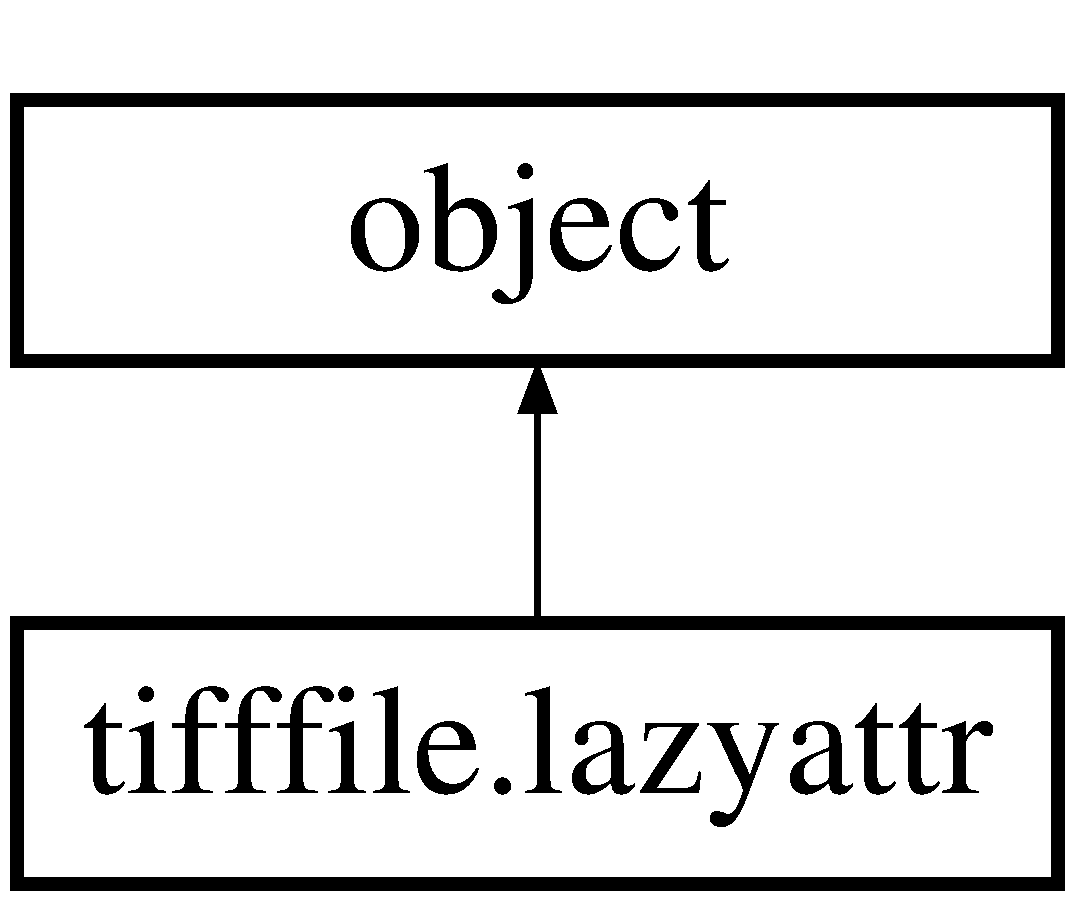
\includegraphics[height=2.000000cm]{classtifffile_1_1lazyattr}
\end{center}
\end{figure}
\subsection*{Public Member Functions}
\begin{DoxyCompactItemize}
\item 
\hypertarget{classtifffile_1_1lazyattr_ae6acbd812e166b92c16d5b76dcac5023}{def {\bfseries \-\_\-\-\_\-init\-\_\-\-\_\-}}\label{classtifffile_1_1lazyattr_ae6acbd812e166b92c16d5b76dcac5023}

\item 
\hypertarget{classtifffile_1_1lazyattr_ab4c827b46c8833a1cb92b6282c8a9365}{def {\bfseries \-\_\-\-\_\-get\-\_\-\-\_\-}}\label{classtifffile_1_1lazyattr_ab4c827b46c8833a1cb92b6282c8a9365}

\end{DoxyCompactItemize}
\subsection*{Public Attributes}
\begin{DoxyCompactItemize}
\item 
\hypertarget{classtifffile_1_1lazyattr_a2d8c47f2babd83fd5d0ca2135a63e6a4}{{\bfseries func}}\label{classtifffile_1_1lazyattr_a2d8c47f2babd83fd5d0ca2135a63e6a4}

\end{DoxyCompactItemize}


\subsection{Detailed Description}
\begin{DoxyVerb}Lazy object attribute whose value is computed on first access.\end{DoxyVerb}
 

The documentation for this class was generated from the following file\-:\begin{DoxyCompactItemize}
\item 
/home/harold/workdir/atrex/\-Software/tifffile.\-py\end{DoxyCompactItemize}

\hypertarget{classmpfit_1_1machar}{\section{mpfit.\-machar Class Reference}
\label{classmpfit_1_1machar}\index{mpfit.\-machar@{mpfit.\-machar}}
}
\subsection*{Public Member Functions}
\begin{DoxyCompactItemize}
\item 
def \hyperlink{classmpfit_1_1machar_a107a955a7c4b29ad883a7c95a564479b}{\-\_\-\-\_\-init\-\_\-\-\_\-}
\end{DoxyCompactItemize}
\subsection*{Public Attributes}
\begin{DoxyCompactItemize}
\item 
\hyperlink{classmpfit_1_1machar_a3f4c542f8c12eadb7fd7899b85e7418f}{machep}
\item 
\hyperlink{classmpfit_1_1machar_ab572a985f979d3940525b5867deafb86}{maxnum}
\item 
\hyperlink{classmpfit_1_1machar_a81a54c7e41c2ef0471983156b9d18b19}{minnum}
\item 
\hyperlink{classmpfit_1_1machar_a038d6337e708014cfb3efedc9fdb4fc8}{maxlog}
\item 
\hyperlink{classmpfit_1_1machar_af01c85a38dbf4a94ae46170e4306baf9}{minlog}
\item 
\hyperlink{classmpfit_1_1machar_ae0d8c6eebbf9deca09bcbc893d5e0428}{rdwarf}
\item 
\hyperlink{classmpfit_1_1machar_ab78cc8c341cd8a39922aa13341be9df9}{rgiant}
\end{DoxyCompactItemize}


\subsection{Constructor \& Destructor Documentation}
\hypertarget{classmpfit_1_1machar_a107a955a7c4b29ad883a7c95a564479b}{\index{mpfit\-::machar@{mpfit\-::machar}!\-\_\-\-\_\-init\-\_\-\-\_\-@{\-\_\-\-\_\-init\-\_\-\-\_\-}}
\index{\-\_\-\-\_\-init\-\_\-\-\_\-@{\-\_\-\-\_\-init\-\_\-\-\_\-}!mpfit::machar@{mpfit\-::machar}}
\subsubsection[{\-\_\-\-\_\-init\-\_\-\-\_\-}]{\setlength{\rightskip}{0pt plus 5cm}def mpfit.\-machar.\-\_\-\-\_\-init\-\_\-\-\_\- (
\begin{DoxyParamCaption}
\item[{}]{self, }
\item[{}]{double = {\ttfamily 1}}
\end{DoxyParamCaption}
)}}\label{classmpfit_1_1machar_a107a955a7c4b29ad883a7c95a564479b}


\subsection{Member Data Documentation}
\hypertarget{classmpfit_1_1machar_a3f4c542f8c12eadb7fd7899b85e7418f}{\index{mpfit\-::machar@{mpfit\-::machar}!machep@{machep}}
\index{machep@{machep}!mpfit::machar@{mpfit\-::machar}}
\subsubsection[{machep}]{\setlength{\rightskip}{0pt plus 5cm}mpfit.\-machar.\-machep}}\label{classmpfit_1_1machar_a3f4c542f8c12eadb7fd7899b85e7418f}
\hypertarget{classmpfit_1_1machar_a038d6337e708014cfb3efedc9fdb4fc8}{\index{mpfit\-::machar@{mpfit\-::machar}!maxlog@{maxlog}}
\index{maxlog@{maxlog}!mpfit::machar@{mpfit\-::machar}}
\subsubsection[{maxlog}]{\setlength{\rightskip}{0pt plus 5cm}mpfit.\-machar.\-maxlog}}\label{classmpfit_1_1machar_a038d6337e708014cfb3efedc9fdb4fc8}
\hypertarget{classmpfit_1_1machar_ab572a985f979d3940525b5867deafb86}{\index{mpfit\-::machar@{mpfit\-::machar}!maxnum@{maxnum}}
\index{maxnum@{maxnum}!mpfit::machar@{mpfit\-::machar}}
\subsubsection[{maxnum}]{\setlength{\rightskip}{0pt plus 5cm}mpfit.\-machar.\-maxnum}}\label{classmpfit_1_1machar_ab572a985f979d3940525b5867deafb86}
\hypertarget{classmpfit_1_1machar_af01c85a38dbf4a94ae46170e4306baf9}{\index{mpfit\-::machar@{mpfit\-::machar}!minlog@{minlog}}
\index{minlog@{minlog}!mpfit::machar@{mpfit\-::machar}}
\subsubsection[{minlog}]{\setlength{\rightskip}{0pt plus 5cm}mpfit.\-machar.\-minlog}}\label{classmpfit_1_1machar_af01c85a38dbf4a94ae46170e4306baf9}
\hypertarget{classmpfit_1_1machar_a81a54c7e41c2ef0471983156b9d18b19}{\index{mpfit\-::machar@{mpfit\-::machar}!minnum@{minnum}}
\index{minnum@{minnum}!mpfit::machar@{mpfit\-::machar}}
\subsubsection[{minnum}]{\setlength{\rightskip}{0pt plus 5cm}mpfit.\-machar.\-minnum}}\label{classmpfit_1_1machar_a81a54c7e41c2ef0471983156b9d18b19}
\hypertarget{classmpfit_1_1machar_ae0d8c6eebbf9deca09bcbc893d5e0428}{\index{mpfit\-::machar@{mpfit\-::machar}!rdwarf@{rdwarf}}
\index{rdwarf@{rdwarf}!mpfit::machar@{mpfit\-::machar}}
\subsubsection[{rdwarf}]{\setlength{\rightskip}{0pt plus 5cm}mpfit.\-machar.\-rdwarf}}\label{classmpfit_1_1machar_ae0d8c6eebbf9deca09bcbc893d5e0428}
\hypertarget{classmpfit_1_1machar_ab78cc8c341cd8a39922aa13341be9df9}{\index{mpfit\-::machar@{mpfit\-::machar}!rgiant@{rgiant}}
\index{rgiant@{rgiant}!mpfit::machar@{mpfit\-::machar}}
\subsubsection[{rgiant}]{\setlength{\rightskip}{0pt plus 5cm}mpfit.\-machar.\-rgiant}}\label{classmpfit_1_1machar_ab78cc8c341cd8a39922aa13341be9df9}


The documentation for this class was generated from the following file\-:\begin{DoxyCompactItemize}
\item 
workdir/atrex/\-Software/\hyperlink{mpfit_8py}{mpfit.\-py}\end{DoxyCompactItemize}

\hypertarget{class_main_peaks_1_1_main_peaks}{\section{Main\-Peaks.\-Main\-Peaks Class Reference}
\label{class_main_peaks_1_1_main_peaks}\index{Main\-Peaks.\-Main\-Peaks@{Main\-Peaks.\-Main\-Peaks}}
}
\subsection*{Public Member Functions}
\begin{DoxyCompactItemize}
\item 
def \hyperlink{class_main_peaks_1_1_main_peaks_a8a133d3ee42e272cee3c30d8a1bb6b56}{\-\_\-\-\_\-init\-\_\-\-\_\-}
\item 
def \hyperlink{class_main_peaks_1_1_main_peaks_a6c85bd1ad41c9737aa86d98e447965b2}{set\-Image}
\item 
def \hyperlink{class_main_peaks_1_1_main_peaks_af353c28f582d469588714fa90f5cefd3}{peak\-Search}
\item 
def \hyperlink{class_main_peaks_1_1_main_peaks_a450255618019c923a86edbe454578f7b}{write\-Peaks\-To\-File}
\end{DoxyCompactItemize}
\subsection*{Public Attributes}
\begin{DoxyCompactItemize}
\item 
\hyperlink{class_main_peaks_1_1_main_peaks_a3154ab9972004f57fe2e423781f07452}{myimage}
\item 
\hyperlink{class_main_peaks_1_1_main_peaks_a5c32a36556e49ae19ef9434048cc4a42}{peaks}
\end{DoxyCompactItemize}


\subsection{Constructor \& Destructor Documentation}
\hypertarget{class_main_peaks_1_1_main_peaks_a8a133d3ee42e272cee3c30d8a1bb6b56}{\index{Main\-Peaks\-::\-Main\-Peaks@{Main\-Peaks\-::\-Main\-Peaks}!\-\_\-\-\_\-init\-\_\-\-\_\-@{\-\_\-\-\_\-init\-\_\-\-\_\-}}
\index{\-\_\-\-\_\-init\-\_\-\-\_\-@{\-\_\-\-\_\-init\-\_\-\-\_\-}!MainPeaks::MainPeaks@{Main\-Peaks\-::\-Main\-Peaks}}
\subsubsection[{\-\_\-\-\_\-init\-\_\-\-\_\-}]{\setlength{\rightskip}{0pt plus 5cm}def Main\-Peaks.\-Main\-Peaks.\-\_\-\-\_\-init\-\_\-\-\_\- (
\begin{DoxyParamCaption}
\item[{}]{self, }
\item[{}]{fname}
\end{DoxyParamCaption}
)}}\label{class_main_peaks_1_1_main_peaks_a8a133d3ee42e272cee3c30d8a1bb6b56}


\subsection{Member Function Documentation}
\hypertarget{class_main_peaks_1_1_main_peaks_af353c28f582d469588714fa90f5cefd3}{\index{Main\-Peaks\-::\-Main\-Peaks@{Main\-Peaks\-::\-Main\-Peaks}!peak\-Search@{peak\-Search}}
\index{peak\-Search@{peak\-Search}!MainPeaks::MainPeaks@{Main\-Peaks\-::\-Main\-Peaks}}
\subsubsection[{peak\-Search}]{\setlength{\rightskip}{0pt plus 5cm}def Main\-Peaks.\-Main\-Peaks.\-peak\-Search (
\begin{DoxyParamCaption}
\item[{}]{self}
\end{DoxyParamCaption}
)}}\label{class_main_peaks_1_1_main_peaks_af353c28f582d469588714fa90f5cefd3}
\hypertarget{class_main_peaks_1_1_main_peaks_a6c85bd1ad41c9737aa86d98e447965b2}{\index{Main\-Peaks\-::\-Main\-Peaks@{Main\-Peaks\-::\-Main\-Peaks}!set\-Image@{set\-Image}}
\index{set\-Image@{set\-Image}!MainPeaks::MainPeaks@{Main\-Peaks\-::\-Main\-Peaks}}
\subsubsection[{set\-Image}]{\setlength{\rightskip}{0pt plus 5cm}def Main\-Peaks.\-Main\-Peaks.\-set\-Image (
\begin{DoxyParamCaption}
\item[{}]{self, }
\item[{}]{fname}
\end{DoxyParamCaption}
)}}\label{class_main_peaks_1_1_main_peaks_a6c85bd1ad41c9737aa86d98e447965b2}
\hypertarget{class_main_peaks_1_1_main_peaks_a450255618019c923a86edbe454578f7b}{\index{Main\-Peaks\-::\-Main\-Peaks@{Main\-Peaks\-::\-Main\-Peaks}!write\-Peaks\-To\-File@{write\-Peaks\-To\-File}}
\index{write\-Peaks\-To\-File@{write\-Peaks\-To\-File}!MainPeaks::MainPeaks@{Main\-Peaks\-::\-Main\-Peaks}}
\subsubsection[{write\-Peaks\-To\-File}]{\setlength{\rightskip}{0pt plus 5cm}def Main\-Peaks.\-Main\-Peaks.\-write\-Peaks\-To\-File (
\begin{DoxyParamCaption}
\item[{}]{self, }
\item[{}]{ascii\-File}
\end{DoxyParamCaption}
)}}\label{class_main_peaks_1_1_main_peaks_a450255618019c923a86edbe454578f7b}


\subsection{Member Data Documentation}
\hypertarget{class_main_peaks_1_1_main_peaks_a3154ab9972004f57fe2e423781f07452}{\index{Main\-Peaks\-::\-Main\-Peaks@{Main\-Peaks\-::\-Main\-Peaks}!myimage@{myimage}}
\index{myimage@{myimage}!MainPeaks::MainPeaks@{Main\-Peaks\-::\-Main\-Peaks}}
\subsubsection[{myimage}]{\setlength{\rightskip}{0pt plus 5cm}Main\-Peaks.\-Main\-Peaks.\-myimage}}\label{class_main_peaks_1_1_main_peaks_a3154ab9972004f57fe2e423781f07452}
\hypertarget{class_main_peaks_1_1_main_peaks_a5c32a36556e49ae19ef9434048cc4a42}{\index{Main\-Peaks\-::\-Main\-Peaks@{Main\-Peaks\-::\-Main\-Peaks}!peaks@{peaks}}
\index{peaks@{peaks}!MainPeaks::MainPeaks@{Main\-Peaks\-::\-Main\-Peaks}}
\subsubsection[{peaks}]{\setlength{\rightskip}{0pt plus 5cm}Main\-Peaks.\-Main\-Peaks.\-peaks}}\label{class_main_peaks_1_1_main_peaks_a5c32a36556e49ae19ef9434048cc4a42}


The documentation for this class was generated from the following file\-:\begin{DoxyCompactItemize}
\item 
workdir/atrex/\-Software/\hyperlink{_main_peaks_8py}{Main\-Peaks.\-py}\end{DoxyCompactItemize}

\hypertarget{classmpfit_1_1mpfit}{\section{mpfit.\-mpfit Class Reference}
\label{classmpfit_1_1mpfit}\index{mpfit.\-mpfit@{mpfit.\-mpfit}}
}
\subsection*{Public Member Functions}
\begin{DoxyCompactItemize}
\item 
def \hyperlink{classmpfit_1_1mpfit_a85f978dd465cf7e718286d24ae6c60a4}{\-\_\-\-\_\-init\-\_\-\-\_\-}
\item 
def \hyperlink{classmpfit_1_1mpfit_a05677996f0b51ba1872c6da189a716b3}{\-\_\-\-\_\-str\-\_\-\-\_\-}
\item 
def \hyperlink{classmpfit_1_1mpfit_a2642766f2780ad122bf6a8da506a3524}{defiter}
\item 
def \hyperlink{classmpfit_1_1mpfit_a4044ca5a6e332785b83426fec482dcf9}{parinfo}
\item 
def \hyperlink{classmpfit_1_1mpfit_a4a57197c1a780d1802d635aaa071ca0c}{call}
\item 
def \hyperlink{classmpfit_1_1mpfit_aacd12e70b3688a26daeece9c2d2f3bf2}{enorm}
\item 
def \hyperlink{classmpfit_1_1mpfit_a4d85cdc05b2d972f319ec1c336337906}{fdjac2}
\item 
def \hyperlink{classmpfit_1_1mpfit_a58e4954f7b62f1e53b2119a3781e03fd}{qrfac}
\item 
def \hyperlink{classmpfit_1_1mpfit_a68e859946e64a6d998b7f48cd0949875}{qrsolv}
\item 
def \hyperlink{classmpfit_1_1mpfit_abb9d174821c887e5d5aa2ca2cc7519f7}{lmpar}
\item 
def \hyperlink{classmpfit_1_1mpfit_a68b9dc3249164597f0d8ed1f6f889ebf}{tie}
\item 
def \hyperlink{classmpfit_1_1mpfit_a217e3eaade969816474f06387c0002ae}{calc\-\_\-covar}
\end{DoxyCompactItemize}
\subsection*{Public Attributes}
\begin{DoxyCompactItemize}
\item 
\hyperlink{classmpfit_1_1mpfit_a0acb816b501c7c62de9b40d51ed3e019}{niter}
\item 
\hyperlink{classmpfit_1_1mpfit_aeeab3c562889cb4fe9d347eeb7e8b40e}{params}
\item 
\hyperlink{classmpfit_1_1mpfit_a6e2df0f73518da9c1bfb3b6c7049bf19}{covar}
\item 
\hyperlink{classmpfit_1_1mpfit_a7fd7c6e0276941f29ae138be862c05fa}{perror}
\item 
\hyperlink{classmpfit_1_1mpfit_a07bef52fd34a9c9d76d605d5d5ff6e6e}{status}
\item 
\hyperlink{classmpfit_1_1mpfit_a358f9f890ac24bb17cf324dd769a69cb}{debug}
\item 
\hyperlink{classmpfit_1_1mpfit_ae0e12388314fd29ceeada36c1f706f53}{errmsg}
\item 
\hyperlink{classmpfit_1_1mpfit_a4a63457ae8102a51227f7ebae4d1d63d}{nfev}
\item 
\hyperlink{classmpfit_1_1mpfit_aef26cc875dbd46374c00332953bb556e}{damp}
\item 
\hyperlink{classmpfit_1_1mpfit_a921637d44c54727c9434aada7f2fc8fb}{dof}
\item 
\hyperlink{classmpfit_1_1mpfit_a69fbce6bf57f692544b35f71d6ae1a07}{fnorm}
\item 
\hyperlink{classmpfit_1_1mpfit_a88c16eda6a0a5ddf3296b1b2d82eba06}{qanytied}
\item 
\hyperlink{classmpfit_1_1mpfit_a121863b0d2d0ffca2d375b7a6f19a567}{ptied}
\item 
\hyperlink{classmpfit_1_1mpfit_a3b940dde9105271118b2e88d9ed88740}{machar}
\item 
\hyperlink{classmpfit_1_1mpfit_ab275d6a4b396b11b4a21d9af891b385f}{blas\-\_\-enorm}
\end{DoxyCompactItemize}


\subsection{Constructor \& Destructor Documentation}
\hypertarget{classmpfit_1_1mpfit_a85f978dd465cf7e718286d24ae6c60a4}{\index{mpfit\-::mpfit@{mpfit\-::mpfit}!\-\_\-\-\_\-init\-\_\-\-\_\-@{\-\_\-\-\_\-init\-\_\-\-\_\-}}
\index{\-\_\-\-\_\-init\-\_\-\-\_\-@{\-\_\-\-\_\-init\-\_\-\-\_\-}!mpfit::mpfit@{mpfit\-::mpfit}}
\subsubsection[{\-\_\-\-\_\-init\-\_\-\-\_\-}]{\setlength{\rightskip}{0pt plus 5cm}def mpfit.\-mpfit.\-\_\-\-\_\-init\-\_\-\-\_\- (
\begin{DoxyParamCaption}
\item[{}]{self, }
\item[{}]{fcn, }
\item[{}]{xall = {\ttfamily None}, }
\item[{}]{functkw = {\ttfamily \{\}}, }
\item[{}]{parinfo = {\ttfamily None}, }
\item[{}]{ftol = {\ttfamily 1.e-\/10}, }
\item[{}]{xtol = {\ttfamily 1.e-\/10}, }
\item[{}]{gtol = {\ttfamily 1.e-\/10}, }
\item[{}]{damp = {\ttfamily 0.}, }
\item[{}]{maxiter = {\ttfamily 200}, }
\item[{}]{factor = {\ttfamily 100.}, }
\item[{}]{nprint = {\ttfamily 1}, }
\item[{}]{iterfunct = {\ttfamily 'default'}, }
\item[{}]{iterkw = {\ttfamily \{\}}, }
\item[{}]{nocovar = {\ttfamily 0}, }
\item[{}]{rescale = {\ttfamily 0}, }
\item[{}]{autoderivative = {\ttfamily 1}, }
\item[{}]{quiet = {\ttfamily 0}, }
\item[{}]{diag = {\ttfamily None}, }
\item[{}]{epsfcn = {\ttfamily None}, }
\item[{}]{debug = {\ttfamily 0}}
\end{DoxyParamCaption}
)}}\label{classmpfit_1_1mpfit_a85f978dd465cf7e718286d24ae6c60a4}
\begin{DoxyVerb}  Inputs:
    fcn:
       The function to be minimized.  The function should return the weighted
       deviations between the model and the data, as described above.

    xall:
       An array of starting values for each of the parameters of the model.
       The number of parameters should be fewer than the number of measurements.

       This parameter is optional if the parinfo keyword is used (but see
       parinfo).  The parinfo keyword provides a mechanism to fix or constrain
       individual parameters.

  Keywords:

     autoderivative:
If this is set, derivatives of the function will be computed
automatically via a finite differencing procedure.  If not set, then
fcn must provide the (analytical) derivatives.
   Default: set (=1)
   NOTE: to supply your own analytical derivatives,
 explicitly pass autoderivative=0

     ftol:
A nonnegative input variable. Termination occurs when both the actual
and predicted relative reductions in the sum of squares are at most
ftol (and status is accordingly set to 1 or 3).  Therefore, ftol
measures the relative error desired in the sum of squares.
   Default: 1E-10

     functkw:
A dictionary which contains the parameters to be passed to the
user-supplied function specified by fcn via the standard Python
keyword dictionary mechanism.  This is the way you can pass additional
data to your user-supplied function without using global variables.

Consider the following example:
   if functkw = {'xval':[1.,2.,3.], 'yval':[1.,4.,9.],
         'errval':[1.,1.,1.] }
then the user supplied function should be declared like this:
   def myfunct(p, fjac=None, xval=None, yval=None, errval=None):

Default: {}   No extra parameters are passed to the user-supplied
      function.

     gtol:
A nonnegative input variable. Termination occurs when the cosine of
the angle between fvec and any column of the jacobian is at most gtol
in absolute value (and status is accordingly set to 4). Therefore,
gtol measures the orthogonality desired between the function vector
and the columns of the jacobian.
   Default: 1e-10

     iterkw:
The keyword arguments to be passed to iterfunct via the dictionary
keyword mechanism.  This should be a dictionary and is similar in
operation to FUNCTKW.
   Default: {}  No arguments are passed.

     iterfunct:
The name of a function to be called upon each NPRINT iteration of the
MPFIT routine.  It should be declared in the following way:
   def iterfunct(myfunct, p, iter, fnorm, functkw=None,
         parinfo=None, quiet=0, dof=None, [iterkw keywords here])
   # perform custom iteration update

iterfunct must accept all three keyword parameters (FUNCTKW, PARINFO
and QUIET).

myfunct:  The user-supplied function to be minimized,
p:      The current set of model parameters
iter:    The iteration number
functkw:  The arguments to be passed to myfunct.
fnorm:  The chi-squared value.
quiet:  Set when no textual output should be printed.
dof:      The number of degrees of freedom, normally the number of points
  less the number of free parameters.
See below for documentation of parinfo.

In implementation, iterfunct can perform updates to the terminal or
graphical user interface, to provide feedback while the fit proceeds.
If the fit is to be stopped for any reason, then iterfunct should return a
a status value between -15 and -1.  Otherwise it should return None
(e.g. no return statement) or 0.
In principle, iterfunct should probably not modify the parameter values,
because it may interfere with the algorithm's stability.  In practice it
is allowed.

Default: an internal routine is used to print the parameter values.

Set iterfunct=None if there is no user-defined routine and you don't
want the internal default routine be called.

     maxiter:
The maximum number of iterations to perform.  If the number is exceeded,
then the status value is set to 5 and MPFIT returns.
Default: 200 iterations

     nocovar:
Set this keyword to prevent the calculation of the covariance matrix
before returning (see COVAR)
Default: clear (=0)  The covariance matrix is returned

     nprint:
The frequency with which iterfunct is called.  A value of 1 indicates
that iterfunct is called with every iteration, while 2 indicates every
other iteration, etc.  Note that several Levenberg-Marquardt attempts
can be made in a single iteration.
Default value: 1

     parinfo
Provides a mechanism for more sophisticated constraints to be placed on
parameter values.  When parinfo is not passed, then it is assumed that
all parameters are free and unconstrained.  Values in parinfo are never
modified during a call to MPFIT.

See description above for the structure of PARINFO.

Default value: None  All parameters are free and unconstrained.

     quiet:
Set this keyword when no textual output should be printed by MPFIT

     damp:
A scalar number, indicating the cut-off value of residuals where
"damping" will occur.  Residuals with magnitudes greater than this
number will be replaced by their hyperbolic tangent.  This partially
mitigates the so-called large residual problem inherent in
least-squares solvers (as for the test problem CURVI,
http://www.maxthis.com/curviex.htm).
A value of 0 indicates no damping.
   Default: 0

Note: DAMP doesn't work with autoderivative=0

     xtol:
A nonnegative input variable. Termination occurs when the relative error
between two consecutive iterates is at most xtol (and status is
accordingly set to 2 or 3).  Therefore, xtol measures the relative error
desired in the approximate solution.
Default: 1E-10

   Outputs:

     Returns an object of type mpfit.  The results are attributes of this class,
     e.g. mpfit.status, mpfit.errmsg, mpfit.params, npfit.niter, mpfit.covar.

     .status
An integer status code is returned.  All values greater than zero can
represent success (however .status == 5 may indicate failure to
converge). It can have one of the following values:

-16
   A parameter or function value has become infinite or an undefined
   number.  This is usually a consequence of numerical overflow in the
   user's model function, which must be avoided.

-15 to -1
   These are error codes that either MYFUNCT or iterfunct may return to
   terminate the fitting process.  Values from -15 to -1 are reserved
   for the user functions and will not clash with MPFIT.

0  Improper input parameters.

1  Both actual and predicted relative reductions in the sum of squares
   are at most ftol.

2  Relative error between two consecutive iterates is at most xtol

3  Conditions for status = 1 and status = 2 both hold.

4  The cosine of the angle between fvec and any column of the jacobian
   is at most gtol in absolute value.

5  The maximum number of iterations has been reached.

6  ftol is too small. No further reduction in the sum of squares is
   possible.

7  xtol is too small. No further improvement in the approximate solution
   x is possible.

8  gtol is too small. fvec is orthogonal to the columns of the jacobian
   to machine precision.

     .fnorm
The value of the summed squared residuals for the returned parameter
values.

     .covar
The covariance matrix for the set of parameters returned by MPFIT.
The matrix is NxN where N is the number of  parameters.  The square root
of the diagonal elements gives the formal 1-sigma statistical errors on
the parameters if errors were treated "properly" in fcn.
Parameter errors are also returned in .perror.

To compute the correlation matrix, pcor, use this example:
   cov = mpfit.covar
   pcor = cov * 0.
   for i in range(n):
      for j in range(n):
 pcor[i,j] = cov[i,j]/sqrt(cov[i,i]*cov[j,j])

If nocovar is set or MPFIT terminated abnormally, then .covar is set to
a scalar with value None.

     .errmsg
A string error or warning message is returned.

     .nfev
The number of calls to MYFUNCT performed.

     .niter
The number of iterations completed.

     .perror
The formal 1-sigma errors in each parameter, computed from the
covariance matrix.  If a parameter is held fixed, or if it touches a
boundary, then the error is reported as zero.

If the fit is unweighted (i.e. no errors were given, or the weights
were uniformly set to unity), then .perror will probably not represent
the true parameter uncertainties.

*If* you can assume that the true reduced chi-squared value is unity --
meaning that the fit is implicitly assumed to be of good quality --
then the estimated parameter uncertainties can be computed by scaling
.perror by the measured chi-squared value.

   dof = len(x) - len(mpfit.params) # deg of freedom
   # scaled uncertainties
   pcerror = mpfit.perror * sqrt(mpfit.fnorm / dof)\end{DoxyVerb}
 

\subsection{Member Function Documentation}
\hypertarget{classmpfit_1_1mpfit_a05677996f0b51ba1872c6da189a716b3}{\index{mpfit\-::mpfit@{mpfit\-::mpfit}!\-\_\-\-\_\-str\-\_\-\-\_\-@{\-\_\-\-\_\-str\-\_\-\-\_\-}}
\index{\-\_\-\-\_\-str\-\_\-\-\_\-@{\-\_\-\-\_\-str\-\_\-\-\_\-}!mpfit::mpfit@{mpfit\-::mpfit}}
\subsubsection[{\-\_\-\-\_\-str\-\_\-\-\_\-}]{\setlength{\rightskip}{0pt plus 5cm}def mpfit.\-mpfit.\-\_\-\-\_\-str\-\_\-\-\_\- (
\begin{DoxyParamCaption}
\item[{}]{self}
\end{DoxyParamCaption}
)}}\label{classmpfit_1_1mpfit_a05677996f0b51ba1872c6da189a716b3}
\hypertarget{classmpfit_1_1mpfit_a217e3eaade969816474f06387c0002ae}{\index{mpfit\-::mpfit@{mpfit\-::mpfit}!calc\-\_\-covar@{calc\-\_\-covar}}
\index{calc\-\_\-covar@{calc\-\_\-covar}!mpfit::mpfit@{mpfit\-::mpfit}}
\subsubsection[{calc\-\_\-covar}]{\setlength{\rightskip}{0pt plus 5cm}def mpfit.\-mpfit.\-calc\-\_\-covar (
\begin{DoxyParamCaption}
\item[{}]{self, }
\item[{}]{rr, }
\item[{}]{ipvt = {\ttfamily None}, }
\item[{}]{tol = {\ttfamily 1.e-\/14}}
\end{DoxyParamCaption}
)}}\label{classmpfit_1_1mpfit_a217e3eaade969816474f06387c0002ae}
\hypertarget{classmpfit_1_1mpfit_a4a57197c1a780d1802d635aaa071ca0c}{\index{mpfit\-::mpfit@{mpfit\-::mpfit}!call@{call}}
\index{call@{call}!mpfit::mpfit@{mpfit\-::mpfit}}
\subsubsection[{call}]{\setlength{\rightskip}{0pt plus 5cm}def mpfit.\-mpfit.\-call (
\begin{DoxyParamCaption}
\item[{}]{self, }
\item[{}]{fcn, }
\item[{}]{x, }
\item[{}]{functkw, }
\item[{}]{fjac = {\ttfamily None}}
\end{DoxyParamCaption}
)}}\label{classmpfit_1_1mpfit_a4a57197c1a780d1802d635aaa071ca0c}
\hypertarget{classmpfit_1_1mpfit_a2642766f2780ad122bf6a8da506a3524}{\index{mpfit\-::mpfit@{mpfit\-::mpfit}!defiter@{defiter}}
\index{defiter@{defiter}!mpfit::mpfit@{mpfit\-::mpfit}}
\subsubsection[{defiter}]{\setlength{\rightskip}{0pt plus 5cm}def mpfit.\-mpfit.\-defiter (
\begin{DoxyParamCaption}
\item[{}]{self, }
\item[{}]{fcn, }
\item[{}]{x, }
\item[{}]{iter, }
\item[{}]{fnorm = {\ttfamily None}, }
\item[{}]{functkw = {\ttfamily None}, }
\item[{}]{quiet = {\ttfamily 0}, }
\item[{}]{iterstop = {\ttfamily None}, }
\item[{}]{parinfo = {\ttfamily None}, }
\item[{}]{format = {\ttfamily None}, }
\item[{}]{pformat = {\ttfamily '\%.10g'}, }
\item[{}]{dof = {\ttfamily 1}}
\end{DoxyParamCaption}
)}}\label{classmpfit_1_1mpfit_a2642766f2780ad122bf6a8da506a3524}
\hypertarget{classmpfit_1_1mpfit_aacd12e70b3688a26daeece9c2d2f3bf2}{\index{mpfit\-::mpfit@{mpfit\-::mpfit}!enorm@{enorm}}
\index{enorm@{enorm}!mpfit::mpfit@{mpfit\-::mpfit}}
\subsubsection[{enorm}]{\setlength{\rightskip}{0pt plus 5cm}def mpfit.\-mpfit.\-enorm (
\begin{DoxyParamCaption}
\item[{}]{self, }
\item[{}]{vec}
\end{DoxyParamCaption}
)}}\label{classmpfit_1_1mpfit_aacd12e70b3688a26daeece9c2d2f3bf2}
\hypertarget{classmpfit_1_1mpfit_a4d85cdc05b2d972f319ec1c336337906}{\index{mpfit\-::mpfit@{mpfit\-::mpfit}!fdjac2@{fdjac2}}
\index{fdjac2@{fdjac2}!mpfit::mpfit@{mpfit\-::mpfit}}
\subsubsection[{fdjac2}]{\setlength{\rightskip}{0pt plus 5cm}def mpfit.\-mpfit.\-fdjac2 (
\begin{DoxyParamCaption}
\item[{}]{self, }
\item[{}]{fcn, }
\item[{}]{x, }
\item[{}]{fvec, }
\item[{}]{step = {\ttfamily None}, }
\item[{}]{ulimited = {\ttfamily None}, }
\item[{}]{ulimit = {\ttfamily None}, }
\item[{}]{dside = {\ttfamily None}, }
\item[{}]{epsfcn = {\ttfamily None}, }
\item[{}]{autoderivative = {\ttfamily 1}, }
\item[{}]{functkw = {\ttfamily None}, }
\item[{}]{xall = {\ttfamily None}, }
\item[{}]{ifree = {\ttfamily None}, }
\item[{}]{dstep = {\ttfamily None}}
\end{DoxyParamCaption}
)}}\label{classmpfit_1_1mpfit_a4d85cdc05b2d972f319ec1c336337906}
\hypertarget{classmpfit_1_1mpfit_abb9d174821c887e5d5aa2ca2cc7519f7}{\index{mpfit\-::mpfit@{mpfit\-::mpfit}!lmpar@{lmpar}}
\index{lmpar@{lmpar}!mpfit::mpfit@{mpfit\-::mpfit}}
\subsubsection[{lmpar}]{\setlength{\rightskip}{0pt plus 5cm}def mpfit.\-mpfit.\-lmpar (
\begin{DoxyParamCaption}
\item[{}]{self, }
\item[{}]{r, }
\item[{}]{ipvt, }
\item[{}]{diag, }
\item[{}]{qtb, }
\item[{}]{delta, }
\item[{}]{x, }
\item[{}]{sdiag, }
\item[{}]{par = {\ttfamily None}}
\end{DoxyParamCaption}
)}}\label{classmpfit_1_1mpfit_abb9d174821c887e5d5aa2ca2cc7519f7}
\hypertarget{classmpfit_1_1mpfit_a4044ca5a6e332785b83426fec482dcf9}{\index{mpfit\-::mpfit@{mpfit\-::mpfit}!parinfo@{parinfo}}
\index{parinfo@{parinfo}!mpfit::mpfit@{mpfit\-::mpfit}}
\subsubsection[{parinfo}]{\setlength{\rightskip}{0pt plus 5cm}def mpfit.\-mpfit.\-parinfo (
\begin{DoxyParamCaption}
\item[{}]{self, }
\item[{}]{parinfo = {\ttfamily None}, }
\item[{}]{key = {\ttfamily 'a'}, }
\item[{}]{default = {\ttfamily None}, }
\item[{}]{n = {\ttfamily 0}}
\end{DoxyParamCaption}
)}}\label{classmpfit_1_1mpfit_a4044ca5a6e332785b83426fec482dcf9}
\hypertarget{classmpfit_1_1mpfit_a58e4954f7b62f1e53b2119a3781e03fd}{\index{mpfit\-::mpfit@{mpfit\-::mpfit}!qrfac@{qrfac}}
\index{qrfac@{qrfac}!mpfit::mpfit@{mpfit\-::mpfit}}
\subsubsection[{qrfac}]{\setlength{\rightskip}{0pt plus 5cm}def mpfit.\-mpfit.\-qrfac (
\begin{DoxyParamCaption}
\item[{}]{self, }
\item[{}]{a, }
\item[{}]{pivot = {\ttfamily 0}}
\end{DoxyParamCaption}
)}}\label{classmpfit_1_1mpfit_a58e4954f7b62f1e53b2119a3781e03fd}
\hypertarget{classmpfit_1_1mpfit_a68e859946e64a6d998b7f48cd0949875}{\index{mpfit\-::mpfit@{mpfit\-::mpfit}!qrsolv@{qrsolv}}
\index{qrsolv@{qrsolv}!mpfit::mpfit@{mpfit\-::mpfit}}
\subsubsection[{qrsolv}]{\setlength{\rightskip}{0pt plus 5cm}def mpfit.\-mpfit.\-qrsolv (
\begin{DoxyParamCaption}
\item[{}]{self, }
\item[{}]{r, }
\item[{}]{ipvt, }
\item[{}]{diag, }
\item[{}]{qtb, }
\item[{}]{sdiag}
\end{DoxyParamCaption}
)}}\label{classmpfit_1_1mpfit_a68e859946e64a6d998b7f48cd0949875}
\hypertarget{classmpfit_1_1mpfit_a68b9dc3249164597f0d8ed1f6f889ebf}{\index{mpfit\-::mpfit@{mpfit\-::mpfit}!tie@{tie}}
\index{tie@{tie}!mpfit::mpfit@{mpfit\-::mpfit}}
\subsubsection[{tie}]{\setlength{\rightskip}{0pt plus 5cm}def mpfit.\-mpfit.\-tie (
\begin{DoxyParamCaption}
\item[{}]{self, }
\item[{}]{p, }
\item[{}]{ptied = {\ttfamily None}}
\end{DoxyParamCaption}
)}}\label{classmpfit_1_1mpfit_a68b9dc3249164597f0d8ed1f6f889ebf}


\subsection{Member Data Documentation}
\hypertarget{classmpfit_1_1mpfit_ab275d6a4b396b11b4a21d9af891b385f}{\index{mpfit\-::mpfit@{mpfit\-::mpfit}!blas\-\_\-enorm@{blas\-\_\-enorm}}
\index{blas\-\_\-enorm@{blas\-\_\-enorm}!mpfit::mpfit@{mpfit\-::mpfit}}
\subsubsection[{blas\-\_\-enorm}]{\setlength{\rightskip}{0pt plus 5cm}mpfit.\-mpfit.\-blas\-\_\-enorm}}\label{classmpfit_1_1mpfit_ab275d6a4b396b11b4a21d9af891b385f}
\hypertarget{classmpfit_1_1mpfit_a6e2df0f73518da9c1bfb3b6c7049bf19}{\index{mpfit\-::mpfit@{mpfit\-::mpfit}!covar@{covar}}
\index{covar@{covar}!mpfit::mpfit@{mpfit\-::mpfit}}
\subsubsection[{covar}]{\setlength{\rightskip}{0pt plus 5cm}mpfit.\-mpfit.\-covar}}\label{classmpfit_1_1mpfit_a6e2df0f73518da9c1bfb3b6c7049bf19}
\hypertarget{classmpfit_1_1mpfit_aef26cc875dbd46374c00332953bb556e}{\index{mpfit\-::mpfit@{mpfit\-::mpfit}!damp@{damp}}
\index{damp@{damp}!mpfit::mpfit@{mpfit\-::mpfit}}
\subsubsection[{damp}]{\setlength{\rightskip}{0pt plus 5cm}mpfit.\-mpfit.\-damp}}\label{classmpfit_1_1mpfit_aef26cc875dbd46374c00332953bb556e}
\hypertarget{classmpfit_1_1mpfit_a358f9f890ac24bb17cf324dd769a69cb}{\index{mpfit\-::mpfit@{mpfit\-::mpfit}!debug@{debug}}
\index{debug@{debug}!mpfit::mpfit@{mpfit\-::mpfit}}
\subsubsection[{debug}]{\setlength{\rightskip}{0pt plus 5cm}mpfit.\-mpfit.\-debug}}\label{classmpfit_1_1mpfit_a358f9f890ac24bb17cf324dd769a69cb}
\hypertarget{classmpfit_1_1mpfit_a921637d44c54727c9434aada7f2fc8fb}{\index{mpfit\-::mpfit@{mpfit\-::mpfit}!dof@{dof}}
\index{dof@{dof}!mpfit::mpfit@{mpfit\-::mpfit}}
\subsubsection[{dof}]{\setlength{\rightskip}{0pt plus 5cm}mpfit.\-mpfit.\-dof}}\label{classmpfit_1_1mpfit_a921637d44c54727c9434aada7f2fc8fb}
\hypertarget{classmpfit_1_1mpfit_ae0e12388314fd29ceeada36c1f706f53}{\index{mpfit\-::mpfit@{mpfit\-::mpfit}!errmsg@{errmsg}}
\index{errmsg@{errmsg}!mpfit::mpfit@{mpfit\-::mpfit}}
\subsubsection[{errmsg}]{\setlength{\rightskip}{0pt plus 5cm}mpfit.\-mpfit.\-errmsg}}\label{classmpfit_1_1mpfit_ae0e12388314fd29ceeada36c1f706f53}
\hypertarget{classmpfit_1_1mpfit_a69fbce6bf57f692544b35f71d6ae1a07}{\index{mpfit\-::mpfit@{mpfit\-::mpfit}!fnorm@{fnorm}}
\index{fnorm@{fnorm}!mpfit::mpfit@{mpfit\-::mpfit}}
\subsubsection[{fnorm}]{\setlength{\rightskip}{0pt plus 5cm}mpfit.\-mpfit.\-fnorm}}\label{classmpfit_1_1mpfit_a69fbce6bf57f692544b35f71d6ae1a07}
\hypertarget{classmpfit_1_1mpfit_a3b940dde9105271118b2e88d9ed88740}{\index{mpfit\-::mpfit@{mpfit\-::mpfit}!machar@{machar}}
\index{machar@{machar}!mpfit::mpfit@{mpfit\-::mpfit}}
\subsubsection[{machar}]{\setlength{\rightskip}{0pt plus 5cm}mpfit.\-mpfit.\-machar}}\label{classmpfit_1_1mpfit_a3b940dde9105271118b2e88d9ed88740}
\hypertarget{classmpfit_1_1mpfit_a4a63457ae8102a51227f7ebae4d1d63d}{\index{mpfit\-::mpfit@{mpfit\-::mpfit}!nfev@{nfev}}
\index{nfev@{nfev}!mpfit::mpfit@{mpfit\-::mpfit}}
\subsubsection[{nfev}]{\setlength{\rightskip}{0pt plus 5cm}mpfit.\-mpfit.\-nfev}}\label{classmpfit_1_1mpfit_a4a63457ae8102a51227f7ebae4d1d63d}
\hypertarget{classmpfit_1_1mpfit_a0acb816b501c7c62de9b40d51ed3e019}{\index{mpfit\-::mpfit@{mpfit\-::mpfit}!niter@{niter}}
\index{niter@{niter}!mpfit::mpfit@{mpfit\-::mpfit}}
\subsubsection[{niter}]{\setlength{\rightskip}{0pt plus 5cm}mpfit.\-mpfit.\-niter}}\label{classmpfit_1_1mpfit_a0acb816b501c7c62de9b40d51ed3e019}
\hypertarget{classmpfit_1_1mpfit_aeeab3c562889cb4fe9d347eeb7e8b40e}{\index{mpfit\-::mpfit@{mpfit\-::mpfit}!params@{params}}
\index{params@{params}!mpfit::mpfit@{mpfit\-::mpfit}}
\subsubsection[{params}]{\setlength{\rightskip}{0pt plus 5cm}mpfit.\-mpfit.\-params}}\label{classmpfit_1_1mpfit_aeeab3c562889cb4fe9d347eeb7e8b40e}
\hypertarget{classmpfit_1_1mpfit_a7fd7c6e0276941f29ae138be862c05fa}{\index{mpfit\-::mpfit@{mpfit\-::mpfit}!perror@{perror}}
\index{perror@{perror}!mpfit::mpfit@{mpfit\-::mpfit}}
\subsubsection[{perror}]{\setlength{\rightskip}{0pt plus 5cm}mpfit.\-mpfit.\-perror}}\label{classmpfit_1_1mpfit_a7fd7c6e0276941f29ae138be862c05fa}
\hypertarget{classmpfit_1_1mpfit_a121863b0d2d0ffca2d375b7a6f19a567}{\index{mpfit\-::mpfit@{mpfit\-::mpfit}!ptied@{ptied}}
\index{ptied@{ptied}!mpfit::mpfit@{mpfit\-::mpfit}}
\subsubsection[{ptied}]{\setlength{\rightskip}{0pt plus 5cm}mpfit.\-mpfit.\-ptied}}\label{classmpfit_1_1mpfit_a121863b0d2d0ffca2d375b7a6f19a567}
\hypertarget{classmpfit_1_1mpfit_a88c16eda6a0a5ddf3296b1b2d82eba06}{\index{mpfit\-::mpfit@{mpfit\-::mpfit}!qanytied@{qanytied}}
\index{qanytied@{qanytied}!mpfit::mpfit@{mpfit\-::mpfit}}
\subsubsection[{qanytied}]{\setlength{\rightskip}{0pt plus 5cm}mpfit.\-mpfit.\-qanytied}}\label{classmpfit_1_1mpfit_a88c16eda6a0a5ddf3296b1b2d82eba06}
\hypertarget{classmpfit_1_1mpfit_a07bef52fd34a9c9d76d605d5d5ff6e6e}{\index{mpfit\-::mpfit@{mpfit\-::mpfit}!status@{status}}
\index{status@{status}!mpfit::mpfit@{mpfit\-::mpfit}}
\subsubsection[{status}]{\setlength{\rightskip}{0pt plus 5cm}mpfit.\-mpfit.\-status}}\label{classmpfit_1_1mpfit_a07bef52fd34a9c9d76d605d5d5ff6e6e}


The documentation for this class was generated from the following file\-:\begin{DoxyCompactItemize}
\item 
workdir/atrex/\-Software/\hyperlink{mpfit_8py}{mpfit.\-py}\end{DoxyCompactItemize}

\hypertarget{classmy_detector_1_1my_detector}{\section{my\-Detector.\-my\-Detector Class Reference}
\label{classmy_detector_1_1my_detector}\index{my\-Detector.\-my\-Detector@{my\-Detector.\-my\-Detector}}
}
Inheritance diagram for my\-Detector.\-my\-Detector\-:\begin{figure}[H]
\begin{center}
\leavevmode
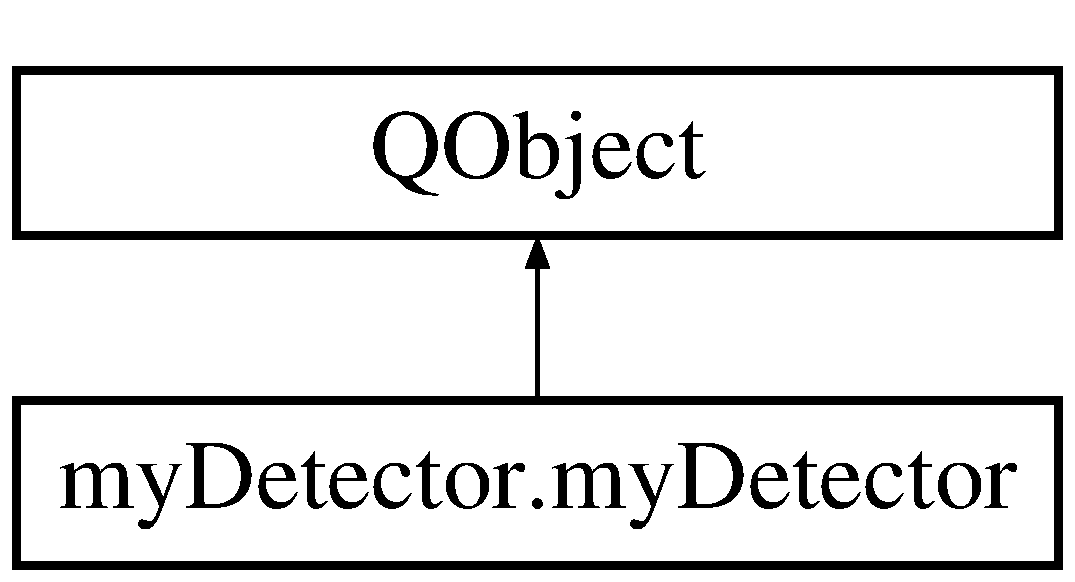
\includegraphics[height=2.000000cm]{classmy_detector_1_1my_detector}
\end{center}
\end{figure}
\subsection*{Public Member Functions}
\begin{DoxyCompactItemize}
\item 
def \hyperlink{classmy_detector_1_1my_detector_a783da80204b3f19403a26284d376fc18}{\-\_\-\-\_\-init\-\_\-\-\_\-}
\item 
def \hyperlink{classmy_detector_1_1my_detector_ad1237b8f9843336bd470eea90068c001}{set\-Top\-Level}
\item 
def \hyperlink{classmy_detector_1_1my_detector_aa9ba5cd92fa49b0935c8cc5a88adf919}{getdist}
\item 
def \hyperlink{classmy_detector_1_1my_detector_a9dbec7a26b92a1d52144dd9fd99e89a7}{setdist}
\item 
def \hyperlink{classmy_detector_1_1my_detector_a73d637fe6d8f0b6685c9ea07e0444b14}{getwavelength}
\item 
def \hyperlink{classmy_detector_1_1my_detector_aa86114f3da1a2f6bf4d8595564654b0c}{setwavelength}
\item 
def \hyperlink{classmy_detector_1_1my_detector_aa70f5dd1888bee1c70eaa1a1410c4cd9}{gettiltom}
\item 
def \hyperlink{classmy_detector_1_1my_detector_a2ab94c7245903209b1ec67fe726727f8}{settiltom}
\item 
def \hyperlink{classmy_detector_1_1my_detector_a5814f9b4c3659e0c3ca527d2c62d0cb5}{gettiltch}
\item 
def \hyperlink{classmy_detector_1_1my_detector_a962ed549d7586e474ad70f18b16ee828}{settiltch}
\item 
def \hyperlink{classmy_detector_1_1my_detector_ae355ac64795c27bec293a55ea1f0f1c5}{getttheta}
\item 
def \hyperlink{classmy_detector_1_1my_detector_a820154c642e5b92a5b7a71d02f0611cd}{setttheta}
\item 
def \hyperlink{classmy_detector_1_1my_detector_af9f5fe17290771ee89f44d61460788c2}{gettwist}
\item 
def \hyperlink{classmy_detector_1_1my_detector_aa347097de35029fb149193660848637f}{settwist}
\item 
def \hyperlink{classmy_detector_1_1my_detector_a77ca154ee209ba6feea760224b0ccc7f}{getbeam\-X\-Y}
\item 
def \hyperlink{classmy_detector_1_1my_detector_a39df1d613aada63ef323aa4a5ca4fa34}{setbeam\-X\-Y}
\item 
def \hyperlink{classmy_detector_1_1my_detector_a9c607c43c8f55baa0c6bd7bf356b17a1}{getpsize\-X\-Y}
\item 
def \hyperlink{classmy_detector_1_1my_detector_a9018d849252b07724e9046a615c27e0b}{setpsize\-X\-Y}
\item 
def \hyperlink{classmy_detector_1_1my_detector_a8f5b1f53fa3905551d797312390be7e9}{getnopix\-X\-Y}
\item 
def \hyperlink{classmy_detector_1_1my_detector_a17e10421e1beb0ace96f0e0075d923d8}{setnopix\-X\-Y}
\item 
def \hyperlink{classmy_detector_1_1my_detector_a47f4a741e9c43ea2ca937b38d26d85bd}{write\-\_\-to\-\_\-file}
\item 
def \hyperlink{classmy_detector_1_1my_detector_a28805fea27eebf5e4b50defd31842d9b}{read\-\_\-from\-\_\-file}
\item 
def \hyperlink{classmy_detector_1_1my_detector_a22f02df85f7dd4f30ab64d7e0b204b6a}{read\-\_\-from\-\_\-text\-\_\-file}
\item 
def \hyperlink{classmy_detector_1_1my_detector_a07bb062a70ceaec37614c8877e6ae659}{write\-\_\-to\-\_\-text\-\_\-file}
\item 
def \hyperlink{classmy_detector_1_1my_detector_a2f7eb213400bfad0ffd110b060ce2469}{calculate\-\_\-tth\-\_\-from\-\_\-pixels}
\item 
def \hyperlink{classmy_detector_1_1my_detector_ad897737f4883453052f916edaee91ac0}{calculate\-\_\-pixels\-\_\-from\-\_\-sd}
\item 
def \hyperlink{classmy_detector_1_1my_detector_a8e63ddf3ddf9aa2972ee936c27788915}{calculate\-\_\-sd\-\_\-from\-\_\-pixels}
\item 
def \hyperlink{classmy_detector_1_1my_detector_abd5c5ca2d3f99a6759a1a9b670ef6b2e}{calculate\-\_\-sd\-\_\-from\-\_\-pixels\-\_\-arr}
\item 
def \hyperlink{classmy_detector_1_1my_detector_a1b53a39b4e53442c2a7f7fb9ee77e156}{tilt\-\_\-mtx}
\item 
def \hyperlink{classmy_detector_1_1my_detector_a91ee215369c918ef83d0c8598daeab46}{gen\-Tilt\-Mtx}
\item 
def \hyperlink{classmy_detector_1_1my_detector_a089663282c90924b0fc4e2f53bb96aa2}{calc2theta}
\item 
def \hyperlink{classmy_detector_1_1my_detector_a10dd4f576fd9e8cd3cbfb45625a74113}{test\-Stuff}
\item 
def \hyperlink{classmy_detector_1_1my_detector_a16783ce90d948c85c5cf0a2930c60a4f}{create\-\_\-ttheta\-\_\-array}
\item 
def \hyperlink{classmy_detector_1_1my_detector_a9558eaedd3456b1705b8962d861f7b1c}{create\-\_\-ttheta\-\_\-array\-\_\-sub}
\item 
def \hyperlink{classmy_detector_1_1my_detector_ab1ec39dedf5ad3f5e49ecacd935632ee}{calc\-Tth\-D\-L\-L}
\item 
def \hyperlink{classmy_detector_1_1my_detector_afc52520eef732679f7ab195a0722a9e7}{generate\-\_\-peaks\-\_\-laue}
\item 
def \hyperlink{classmy_detector_1_1my_detector_ab1ec39dedf5ad3f5e49ecacd935632ee}{calc\-Tth\-D\-L\-L}
\item 
def \hyperlink{classmy_detector_1_1my_detector_ae6bc52229c1afb9e5f4d386f65436609}{thread\-Done\-Slot}
\item 
def \hyperlink{classmy_detector_1_1my_detector_a32e75eff3dbfa9bd7aa2c52c35dc5ed9}{calculate\-\_\-pixels\-\_\-from\-\_\-xyz}
\item 
def \hyperlink{classmy_detector_1_1my_detector_a6c37e75cc10b463055607b353c08906a}{generate\-Rot\-Matrix}
\item 
def \hyperlink{classmy_detector_1_1my_detector_ae044536621ae1d67732986d2786e89eb}{calculate\-\_\-psi\-\_\-angles}
\item 
def \hyperlink{classmy_detector_1_1my_detector_a4a11ce6f14f52e3cf63340d91dc819db}{generate\-\_\-all\-\_\-peaks}
\item 
def \hyperlink{classmy_detector_1_1my_detector_ae56669397e5b8160425c0043ce0bd10f}{read\-\_\-kappa\-\_\-and\-\_\-ttheta}
\item 
def \hyperlink{classmy_detector_1_1my_detector_aa07cdad98650ea99584f29742742c5c5}{test\-Calibration}
\begin{DoxyCompactList}\small\item\em called when test detector cal button is clicked4 \end{DoxyCompactList}\item 
def \hyperlink{classmy_detector_1_1my_detector_a770f58d5ad78d470084f5644ae55865c}{local\-\_\-background}
\item 
def \hyperlink{classmy_detector_1_1my_detector_a3870200120d08278f2f015534ca4557d}{compdist}
\begin{DoxyCompactList}\small\item\em compdist -\/ function to return something from the other pos is two element vector ff is array of tuples, being coords of calib marks returns an npt array with each element being the distance of that point from that specified by pos \end{DoxyCompactList}\item 
def \hyperlink{classmy_detector_1_1my_detector_aeef331d798559cfc9957b453c0db4f1d}{xy\-\_\-from\-\_\-ind}
\end{DoxyCompactItemize}
\subsection*{Static Public Member Functions}
\begin{DoxyCompactItemize}
\item 
def \hyperlink{classmy_detector_1_1my_detector_af1fe29daf9b0c65bb59dbee747583619}{calculate\-\_\-sd\-\_\-from\-\_\-hl}
\end{DoxyCompactItemize}
\subsection*{Public Attributes}
\begin{DoxyCompactItemize}
\item 
\hyperlink{classmy_detector_1_1my_detector_a2246cf4b56f098e953bad790b34f668f}{dist}
\item 
\hyperlink{classmy_detector_1_1my_detector_ac7a646e99083103ff8ae1ae88755dbf8}{beamx}
\item 
\hyperlink{classmy_detector_1_1my_detector_a1a4c1ea459d9cb1d299af5a37484974f}{beamy}
\item 
\hyperlink{classmy_detector_1_1my_detector_aee1c732a56fbddef76f8b8b654d8b67a}{psizex}
\item 
\hyperlink{classmy_detector_1_1my_detector_ac4bb2831ee384d8f59c2ccabf72927f1}{psizey}
\item 
\hyperlink{classmy_detector_1_1my_detector_ae7c12b4ce74cc80a85dae3843f8b764c}{nopixx}
\item 
\hyperlink{classmy_detector_1_1my_detector_a3e60d490ee58d6c5d8ccb7a7a7f24c2e}{nopixy}
\item 
\hyperlink{classmy_detector_1_1my_detector_a339da3a9ba68962c6acd24de484c4c36}{twist}
\item 
\hyperlink{classmy_detector_1_1my_detector_a1c5fb06d769d966ed7fa68b1281b6c6b}{alpha}
\item 
\hyperlink{classmy_detector_1_1my_detector_a950f054dd5d673bb9e005999ef3c1194}{angle}
\item 
\hyperlink{classmy_detector_1_1my_detector_a6c9f97cb6f39f36a0abc0eb938f4270b}{tiltom}
\item 
\hyperlink{classmy_detector_1_1my_detector_aad991ce64666053ea938c784cb2f9783}{tiltch}
\item 
\hyperlink{classmy_detector_1_1my_detector_a9fa295f86db4b7e509856d87f4181cb0}{ttheta}
\item 
\hyperlink{classmy_detector_1_1my_detector_a72cda77b7147f0d187e6540d8c6cb5c2}{wavelength}
\item 
\hyperlink{classmy_detector_1_1my_detector_a854d0f8e848ba2cbc9c4b85ed6e1e1fc}{gonio}
\item 
\hyperlink{classmy_detector_1_1my_detector_abe190122cecdd8f6918d99a03e42701b}{ttheta\-Arr}
\item 
\hyperlink{classmy_detector_1_1my_detector_a7ad466d4bc49ffc4f1a63644c05f1e96}{ttheta\-Bin}
\item 
\hyperlink{classmy_detector_1_1my_detector_aa26398c983b1e7bb378c053430dfb223}{thread\-Done}
\item 
\hyperlink{classmy_detector_1_1my_detector_ae8662acfdbb97b09a6a94523c1181c4e}{Calc\-Theta}
\item 
\hyperlink{classmy_detector_1_1my_detector_a4b106f3ede93bdcd542ab92970bf05bd}{eqprox}
\item 
\hyperlink{classmy_detector_1_1my_detector_a974a82a8a03332b7a567195ec72ad536}{eqproxfine}
\item 
\hyperlink{classmy_detector_1_1my_detector_a496d6c743310d5e8e41b76c857a3ca6f}{top\-Level}
\item 
\hyperlink{classmy_detector_1_1my_detector_aab668b653bad5aa19af675ed93657412}{wavelengtht}
\item 
\hyperlink{classmy_detector_1_1my_detector_ab44d802a6ebf15dc13c349aa798769bd}{ttwist}
\item 
\hyperlink{classmy_detector_1_1my_detector_a8e38cb0a0ede5e4a0a35900341a89591}{tiltmtx}
\item 
\hyperlink{classmy_detector_1_1my_detector_a5f0eaea4e672ec7ecc8d7a6f469e8f82}{tth}
\end{DoxyCompactItemize}
\subsection*{Static Public Attributes}
\begin{DoxyCompactItemize}
\item 
tuple \hyperlink{classmy_detector_1_1my_detector_a83320d2b6159a6b1bc8c053dbfff9bd7}{t\-Done} = Qt\-Core.\-pyqt\-Signal(int)
\item 
tuple \hyperlink{classmy_detector_1_1my_detector_a22ed0aa2e098b8d4d99aefda27475b0d}{t\-Done\-All} = Qt\-Core.\-pyqt\-Signal()
\item 
tuple \hyperlink{classmy_detector_1_1my_detector_a56d596ddc38ea76426625c66e958f597}{cal\-Peaks} = Qt\-Core.\-pyqt\-Signal()
\item 
float \hyperlink{classmy_detector_1_1my_detector_a2e2dfccba7a271626bf2569bcd4230f0}{en} = 37.\-077
\item 
int \hyperlink{classmy_detector_1_1my_detector_ae401cd79076e16e17387d857aa582485}{cut} = 30
\item 
float \hyperlink{classmy_detector_1_1my_detector_a52b6987c8b523fb62551aef4c8915c70}{dist\-\_\-tol} = 1.\-8
\item 
tuple \hyperlink{classmy_detector_1_1my_detector_a47317ecbf510f2824ec6cde297d1b49e}{Iov\-S} = self.\-top\-Level.\-ui.\-det\-\_\-snr\-L\-E.\-text()
\item 
float \hyperlink{classmy_detector_1_1my_detector_a236fc1245269dda1ad8eb67c429d4ea7}{start\-\_\-dist} = self.\-dist-\/self.\-dist$\ast$0.\-5
\item 
int \hyperlink{classmy_detector_1_1my_detector_ad533e746d764e752d9e0d29624b5b8ea}{end\-\_\-dist} = self.\-dist+self.\-dist$\ast$.\-5
\item 
tuple \hyperlink{classmy_detector_1_1my_detector_a410f74814a76fe6a1def53b340335fa7}{imarr} = cgd.\-congrid(myim.\-im\-Array, \mbox{[}500, 500\mbox{]})
\item 
tuple \hyperlink{classmy_detector_1_1my_detector_a5073be601ea77b2b69921ccf0de09f95}{zarr} = np.\-zeros((500,500),dtype=np.\-uint8)
\item 
tuple \hyperlink{classmy_detector_1_1my_detector_aab7c6d5294ad55f8124b65bbfbb2a5c8}{bg} = self.\-local\-\_\-background(\hyperlink{classmy_detector_1_1my_detector_a410f74814a76fe6a1def53b340335fa7}{imarr})
\item 
\hyperlink{classmy_detector_1_1my_detector_a8d151e9e0479b3bed1067c7f3bcf35e0}{hpf} = \hyperlink{classmy_detector_1_1my_detector_a410f74814a76fe6a1def53b340335fa7}{imarr}/\hyperlink{classmy_detector_1_1my_detector_aab7c6d5294ad55f8124b65bbfbb2a5c8}{bg}
\item 
tuple \hyperlink{classmy_detector_1_1my_detector_a386c22e4c8877c163e1c1855ac602d08}{nn} = len(self.\-ff\mbox{[}0\mbox{]})
\item 
tuple \hyperlink{classmy_detector_1_1my_detector_afcb68bb2db834b6bb8c53cb194cf92bf}{h} = np.\-zeros((100,100), dtype=np.\-float32)
\begin{DoxyCompactList}\small\item\em equal proximity coarse search in 5 pixel steps \end{DoxyCompactList}\item 
tuple \hyperlink{classmy_detector_1_1my_detector_a043b9a79c751351b6d34bcf8f0d415ca}{dist} = self.\-compdist(self.\-ff, \mbox{[}j$\ast$5,i$\ast$5\mbox{]})
\item 
tuple \hyperlink{classmy_detector_1_1my_detector_a7527caeb614bc6fe04eeb93654826835}{mx} = dist.\-max()
\item 
tuple \hyperlink{classmy_detector_1_1my_detector_a9b4d1ba192592e66b106294a29e570fa}{mn} = dist.\-min()
\item 
tuple \hyperlink{classmy_detector_1_1my_detector_ab1ca2803f8b16b976504a260af1ec86b}{nbins} = int(dist.\-max() -\/ dist.\-min()+1)
\item 
tuple \hyperlink{classmy_detector_1_1my_detector_a751d25cb37c9899a46a52dab5f032ddd}{maxsub} = np.\-argmax(\hyperlink{classmy_detector_1_1my_detector_afcb68bb2db834b6bb8c53cb194cf92bf}{h})
\item 
int \hyperlink{classmy_detector_1_1my_detector_a12a6741173b6bd3474e420c671d191e7}{maxrow} = \hyperlink{classmy_detector_1_1my_detector_a751d25cb37c9899a46a52dab5f032ddd}{maxsub}/100
\item 
int \hyperlink{classmy_detector_1_1my_detector_afc1018938cfcc881d1bf17950b2dece6}{maxcol} = \hyperlink{classmy_detector_1_1my_detector_a751d25cb37c9899a46a52dab5f032ddd}{maxsub}-\/\hyperlink{classmy_detector_1_1my_detector_a12a6741173b6bd3474e420c671d191e7}{maxrow}$\ast$100
\item 
tuple \hyperlink{classmy_detector_1_1my_detector_aeb28c7375533c3ec81727b7176f116ed}{xy} = self.\-xy\-\_\-from\-\_\-ind(11,11,\hyperlink{classmy_detector_1_1my_detector_a751d25cb37c9899a46a52dab5f032ddd}{maxsub})
\item 
tuple \hyperlink{classmy_detector_1_1my_detector_a6a2f55541520bde064608b1a3c5aec7a}{maxrow} = maxrow+(\hyperlink{classmy_detector_1_1my_detector_aeb28c7375533c3ec81727b7176f116ed}{xy}\mbox{[}0\mbox{]} -\/ 5)
\item 
tuple \hyperlink{classmy_detector_1_1my_detector_a96cedce1e5c66aaeae9d1d8267e74e0c}{maxcol} = maxcol+(\hyperlink{classmy_detector_1_1my_detector_aeb28c7375533c3ec81727b7176f116ed}{xy}\mbox{[}1\mbox{]} -\/ 5)
\item 
list \hyperlink{classmy_detector_1_1my_detector_ac41c95e8050c844f716b64f39fdc65fc}{xy0} = \mbox{[}\hyperlink{classmy_detector_1_1my_detector_a12a6741173b6bd3474e420c671d191e7}{maxrow}, \hyperlink{classmy_detector_1_1my_detector_afc1018938cfcc881d1bf17950b2dece6}{maxcol}\mbox{]}
\end{DoxyCompactItemize}


\subsection{Constructor \& Destructor Documentation}
\hypertarget{classmy_detector_1_1my_detector_a783da80204b3f19403a26284d376fc18}{\index{my\-Detector\-::my\-Detector@{my\-Detector\-::my\-Detector}!\-\_\-\-\_\-init\-\_\-\-\_\-@{\-\_\-\-\_\-init\-\_\-\-\_\-}}
\index{\-\_\-\-\_\-init\-\_\-\-\_\-@{\-\_\-\-\_\-init\-\_\-\-\_\-}!myDetector::myDetector@{my\-Detector\-::my\-Detector}}
\subsubsection[{\-\_\-\-\_\-init\-\_\-\-\_\-}]{\setlength{\rightskip}{0pt plus 5cm}def my\-Detector.\-my\-Detector.\-\_\-\-\_\-init\-\_\-\-\_\- (
\begin{DoxyParamCaption}
\item[{}]{self}
\end{DoxyParamCaption}
)}}\label{classmy_detector_1_1my_detector_a783da80204b3f19403a26284d376fc18}


\subsection{Member Function Documentation}
\hypertarget{classmy_detector_1_1my_detector_a089663282c90924b0fc4e2f53bb96aa2}{\index{my\-Detector\-::my\-Detector@{my\-Detector\-::my\-Detector}!calc2theta@{calc2theta}}
\index{calc2theta@{calc2theta}!myDetector::myDetector@{my\-Detector\-::my\-Detector}}
\subsubsection[{calc2theta}]{\setlength{\rightskip}{0pt plus 5cm}def my\-Detector.\-my\-Detector.\-calc2theta (
\begin{DoxyParamCaption}
\item[{}]{self, }
\item[{}]{save\-Flag}
\end{DoxyParamCaption}
)}}\label{classmy_detector_1_1my_detector_a089663282c90924b0fc4e2f53bb96aa2}
\hypertarget{classmy_detector_1_1my_detector_ab1ec39dedf5ad3f5e49ecacd935632ee}{\index{my\-Detector\-::my\-Detector@{my\-Detector\-::my\-Detector}!calc\-Tth\-D\-L\-L@{calc\-Tth\-D\-L\-L}}
\index{calc\-Tth\-D\-L\-L@{calc\-Tth\-D\-L\-L}!myDetector::myDetector@{my\-Detector\-::my\-Detector}}
\subsubsection[{calc\-Tth\-D\-L\-L}]{\setlength{\rightskip}{0pt plus 5cm}def my\-Detector.\-my\-Detector.\-calc\-Tth\-D\-L\-L (
\begin{DoxyParamCaption}
\item[{}]{self}
\end{DoxyParamCaption}
)}}\label{classmy_detector_1_1my_detector_ab1ec39dedf5ad3f5e49ecacd935632ee}
\hypertarget{classmy_detector_1_1my_detector_ab1ec39dedf5ad3f5e49ecacd935632ee}{\index{my\-Detector\-::my\-Detector@{my\-Detector\-::my\-Detector}!calc\-Tth\-D\-L\-L@{calc\-Tth\-D\-L\-L}}
\index{calc\-Tth\-D\-L\-L@{calc\-Tth\-D\-L\-L}!myDetector::myDetector@{my\-Detector\-::my\-Detector}}
\subsubsection[{calc\-Tth\-D\-L\-L}]{\setlength{\rightskip}{0pt plus 5cm}def my\-Detector.\-my\-Detector.\-calc\-Tth\-D\-L\-L (
\begin{DoxyParamCaption}
\item[{}]{self}
\end{DoxyParamCaption}
)}}\label{classmy_detector_1_1my_detector_ab1ec39dedf5ad3f5e49ecacd935632ee}
\hypertarget{classmy_detector_1_1my_detector_ad897737f4883453052f916edaee91ac0}{\index{my\-Detector\-::my\-Detector@{my\-Detector\-::my\-Detector}!calculate\-\_\-pixels\-\_\-from\-\_\-sd@{calculate\-\_\-pixels\-\_\-from\-\_\-sd}}
\index{calculate\-\_\-pixels\-\_\-from\-\_\-sd@{calculate\-\_\-pixels\-\_\-from\-\_\-sd}!myDetector::myDetector@{my\-Detector\-::my\-Detector}}
\subsubsection[{calculate\-\_\-pixels\-\_\-from\-\_\-sd}]{\setlength{\rightskip}{0pt plus 5cm}def my\-Detector.\-my\-Detector.\-calculate\-\_\-pixels\-\_\-from\-\_\-sd (
\begin{DoxyParamCaption}
\item[{}]{self, }
\item[{}]{sd, }
\item[{}]{gonio}
\end{DoxyParamCaption}
)}}\label{classmy_detector_1_1my_detector_ad897737f4883453052f916edaee91ac0}
\hypertarget{classmy_detector_1_1my_detector_a32e75eff3dbfa9bd7aa2c52c35dc5ed9}{\index{my\-Detector\-::my\-Detector@{my\-Detector\-::my\-Detector}!calculate\-\_\-pixels\-\_\-from\-\_\-xyz@{calculate\-\_\-pixels\-\_\-from\-\_\-xyz}}
\index{calculate\-\_\-pixels\-\_\-from\-\_\-xyz@{calculate\-\_\-pixels\-\_\-from\-\_\-xyz}!myDetector::myDetector@{my\-Detector\-::my\-Detector}}
\subsubsection[{calculate\-\_\-pixels\-\_\-from\-\_\-xyz}]{\setlength{\rightskip}{0pt plus 5cm}def my\-Detector.\-my\-Detector.\-calculate\-\_\-pixels\-\_\-from\-\_\-xyz (
\begin{DoxyParamCaption}
\item[{}]{self, }
\item[{}]{xyz, }
\item[{}]{gonio}
\end{DoxyParamCaption}
)}}\label{classmy_detector_1_1my_detector_a32e75eff3dbfa9bd7aa2c52c35dc5ed9}
\hypertarget{classmy_detector_1_1my_detector_ae044536621ae1d67732986d2786e89eb}{\index{my\-Detector\-::my\-Detector@{my\-Detector\-::my\-Detector}!calculate\-\_\-psi\-\_\-angles@{calculate\-\_\-psi\-\_\-angles}}
\index{calculate\-\_\-psi\-\_\-angles@{calculate\-\_\-psi\-\_\-angles}!myDetector::myDetector@{my\-Detector\-::my\-Detector}}
\subsubsection[{calculate\-\_\-psi\-\_\-angles}]{\setlength{\rightskip}{0pt plus 5cm}def my\-Detector.\-my\-Detector.\-calculate\-\_\-psi\-\_\-angles (
\begin{DoxyParamCaption}
\item[{}]{self, }
\item[{}]{gonio, }
\item[{}]{pix}
\end{DoxyParamCaption}
)}}\label{classmy_detector_1_1my_detector_ae044536621ae1d67732986d2786e89eb}
\hypertarget{classmy_detector_1_1my_detector_af1fe29daf9b0c65bb59dbee747583619}{\index{my\-Detector\-::my\-Detector@{my\-Detector\-::my\-Detector}!calculate\-\_\-sd\-\_\-from\-\_\-hl@{calculate\-\_\-sd\-\_\-from\-\_\-hl}}
\index{calculate\-\_\-sd\-\_\-from\-\_\-hl@{calculate\-\_\-sd\-\_\-from\-\_\-hl}!myDetector::myDetector@{my\-Detector\-::my\-Detector}}
\subsubsection[{calculate\-\_\-sd\-\_\-from\-\_\-hl}]{\setlength{\rightskip}{0pt plus 5cm}def my\-Detector.\-my\-Detector.\-calculate\-\_\-sd\-\_\-from\-\_\-hl (
\begin{DoxyParamCaption}
\item[{}]{hl}
\end{DoxyParamCaption}
)\hspace{0.3cm}{\ttfamily [static]}}}\label{classmy_detector_1_1my_detector_af1fe29daf9b0c65bb59dbee747583619}
\hypertarget{classmy_detector_1_1my_detector_a8e63ddf3ddf9aa2972ee936c27788915}{\index{my\-Detector\-::my\-Detector@{my\-Detector\-::my\-Detector}!calculate\-\_\-sd\-\_\-from\-\_\-pixels@{calculate\-\_\-sd\-\_\-from\-\_\-pixels}}
\index{calculate\-\_\-sd\-\_\-from\-\_\-pixels@{calculate\-\_\-sd\-\_\-from\-\_\-pixels}!myDetector::myDetector@{my\-Detector\-::my\-Detector}}
\subsubsection[{calculate\-\_\-sd\-\_\-from\-\_\-pixels}]{\setlength{\rightskip}{0pt plus 5cm}def my\-Detector.\-my\-Detector.\-calculate\-\_\-sd\-\_\-from\-\_\-pixels (
\begin{DoxyParamCaption}
\item[{}]{self, }
\item[{}]{pix, }
\item[{}]{gonio}
\end{DoxyParamCaption}
)}}\label{classmy_detector_1_1my_detector_a8e63ddf3ddf9aa2972ee936c27788915}
\hypertarget{classmy_detector_1_1my_detector_abd5c5ca2d3f99a6759a1a9b670ef6b2e}{\index{my\-Detector\-::my\-Detector@{my\-Detector\-::my\-Detector}!calculate\-\_\-sd\-\_\-from\-\_\-pixels\-\_\-arr@{calculate\-\_\-sd\-\_\-from\-\_\-pixels\-\_\-arr}}
\index{calculate\-\_\-sd\-\_\-from\-\_\-pixels\-\_\-arr@{calculate\-\_\-sd\-\_\-from\-\_\-pixels\-\_\-arr}!myDetector::myDetector@{my\-Detector\-::my\-Detector}}
\subsubsection[{calculate\-\_\-sd\-\_\-from\-\_\-pixels\-\_\-arr}]{\setlength{\rightskip}{0pt plus 5cm}def my\-Detector.\-my\-Detector.\-calculate\-\_\-sd\-\_\-from\-\_\-pixels\-\_\-arr (
\begin{DoxyParamCaption}
\item[{}]{self, }
\item[{}]{pix, }
\item[{}]{gonio}
\end{DoxyParamCaption}
)}}\label{classmy_detector_1_1my_detector_abd5c5ca2d3f99a6759a1a9b670ef6b2e}
\hypertarget{classmy_detector_1_1my_detector_a2f7eb213400bfad0ffd110b060ce2469}{\index{my\-Detector\-::my\-Detector@{my\-Detector\-::my\-Detector}!calculate\-\_\-tth\-\_\-from\-\_\-pixels@{calculate\-\_\-tth\-\_\-from\-\_\-pixels}}
\index{calculate\-\_\-tth\-\_\-from\-\_\-pixels@{calculate\-\_\-tth\-\_\-from\-\_\-pixels}!myDetector::myDetector@{my\-Detector\-::my\-Detector}}
\subsubsection[{calculate\-\_\-tth\-\_\-from\-\_\-pixels}]{\setlength{\rightskip}{0pt plus 5cm}def my\-Detector.\-my\-Detector.\-calculate\-\_\-tth\-\_\-from\-\_\-pixels (
\begin{DoxyParamCaption}
\item[{}]{self, }
\item[{}]{pix, }
\item[{}]{gonio}
\end{DoxyParamCaption}
)}}\label{classmy_detector_1_1my_detector_a2f7eb213400bfad0ffd110b060ce2469}
\hypertarget{classmy_detector_1_1my_detector_a3870200120d08278f2f015534ca4557d}{\index{my\-Detector\-::my\-Detector@{my\-Detector\-::my\-Detector}!compdist@{compdist}}
\index{compdist@{compdist}!myDetector::myDetector@{my\-Detector\-::my\-Detector}}
\subsubsection[{compdist}]{\setlength{\rightskip}{0pt plus 5cm}def my\-Detector.\-my\-Detector.\-compdist (
\begin{DoxyParamCaption}
\item[{}]{self, }
\item[{}]{ff, }
\item[{}]{pos}
\end{DoxyParamCaption}
)}}\label{classmy_detector_1_1my_detector_a3870200120d08278f2f015534ca4557d}


compdist -\/ function to return something from the other pos is two element vector ff is array of tuples, being coords of calib marks returns an npt array with each element being the distance of that point from that specified by pos 

\hypertarget{classmy_detector_1_1my_detector_a16783ce90d948c85c5cf0a2930c60a4f}{\index{my\-Detector\-::my\-Detector@{my\-Detector\-::my\-Detector}!create\-\_\-ttheta\-\_\-array@{create\-\_\-ttheta\-\_\-array}}
\index{create\-\_\-ttheta\-\_\-array@{create\-\_\-ttheta\-\_\-array}!myDetector::myDetector@{my\-Detector\-::my\-Detector}}
\subsubsection[{create\-\_\-ttheta\-\_\-array}]{\setlength{\rightskip}{0pt plus 5cm}def my\-Detector.\-my\-Detector.\-create\-\_\-ttheta\-\_\-array (
\begin{DoxyParamCaption}
\item[{}]{self, }
\item[{}]{xysize}
\end{DoxyParamCaption}
)}}\label{classmy_detector_1_1my_detector_a16783ce90d948c85c5cf0a2930c60a4f}
\hypertarget{classmy_detector_1_1my_detector_a9558eaedd3456b1705b8962d861f7b1c}{\index{my\-Detector\-::my\-Detector@{my\-Detector\-::my\-Detector}!create\-\_\-ttheta\-\_\-array\-\_\-sub@{create\-\_\-ttheta\-\_\-array\-\_\-sub}}
\index{create\-\_\-ttheta\-\_\-array\-\_\-sub@{create\-\_\-ttheta\-\_\-array\-\_\-sub}!myDetector::myDetector@{my\-Detector\-::my\-Detector}}
\subsubsection[{create\-\_\-ttheta\-\_\-array\-\_\-sub}]{\setlength{\rightskip}{0pt plus 5cm}def my\-Detector.\-my\-Detector.\-create\-\_\-ttheta\-\_\-array\-\_\-sub (
\begin{DoxyParamCaption}
\item[{}]{self, }
\item[{}]{ysize, }
\item[{}]{xsize, }
\item[{}]{starty, }
\item[{}]{startx, }
\item[{}]{tnum}
\end{DoxyParamCaption}
)}}\label{classmy_detector_1_1my_detector_a9558eaedd3456b1705b8962d861f7b1c}
\hypertarget{classmy_detector_1_1my_detector_a4a11ce6f14f52e3cf63340d91dc819db}{\index{my\-Detector\-::my\-Detector@{my\-Detector\-::my\-Detector}!generate\-\_\-all\-\_\-peaks@{generate\-\_\-all\-\_\-peaks}}
\index{generate\-\_\-all\-\_\-peaks@{generate\-\_\-all\-\_\-peaks}!myDetector::myDetector@{my\-Detector\-::my\-Detector}}
\subsubsection[{generate\-\_\-all\-\_\-peaks}]{\setlength{\rightskip}{0pt plus 5cm}def my\-Detector.\-my\-Detector.\-generate\-\_\-all\-\_\-peaks (
\begin{DoxyParamCaption}
\item[{}]{self, }
\item[{}]{ub, }
\item[{}]{pktable, }
\item[{}]{wv, }
\item[{}]{pred, }
\item[{}]{exti, }
\item[{}]{dac\-\_\-open, }
\item[{}]{box}
\end{DoxyParamCaption}
)}}\label{classmy_detector_1_1my_detector_a4a11ce6f14f52e3cf63340d91dc819db}
\hypertarget{classmy_detector_1_1my_detector_afc52520eef732679f7ab195a0722a9e7}{\index{my\-Detector\-::my\-Detector@{my\-Detector\-::my\-Detector}!generate\-\_\-peaks\-\_\-laue@{generate\-\_\-peaks\-\_\-laue}}
\index{generate\-\_\-peaks\-\_\-laue@{generate\-\_\-peaks\-\_\-laue}!myDetector::myDetector@{my\-Detector\-::my\-Detector}}
\subsubsection[{generate\-\_\-peaks\-\_\-laue}]{\setlength{\rightskip}{0pt plus 5cm}def my\-Detector.\-my\-Detector.\-generate\-\_\-peaks\-\_\-laue (
\begin{DoxyParamCaption}
\item[{}]{self, }
\item[{}]{ub, }
\item[{}]{optable, }
\item[{}]{pred, }
\item[{}]{en, }
\item[{}]{exti, }
\item[{}]{D\-A\-C\-\_\-open}
\end{DoxyParamCaption}
)}}\label{classmy_detector_1_1my_detector_afc52520eef732679f7ab195a0722a9e7}
\hypertarget{classmy_detector_1_1my_detector_a6c37e75cc10b463055607b353c08906a}{\index{my\-Detector\-::my\-Detector@{my\-Detector\-::my\-Detector}!generate\-Rot\-Matrix@{generate\-Rot\-Matrix}}
\index{generate\-Rot\-Matrix@{generate\-Rot\-Matrix}!myDetector::myDetector@{my\-Detector\-::my\-Detector}}
\subsubsection[{generate\-Rot\-Matrix}]{\setlength{\rightskip}{0pt plus 5cm}def my\-Detector.\-my\-Detector.\-generate\-Rot\-Matrix (
\begin{DoxyParamCaption}
\item[{}]{self, }
\item[{}]{axisnumber, }
\item[{}]{angle}
\end{DoxyParamCaption}
)}}\label{classmy_detector_1_1my_detector_a6c37e75cc10b463055607b353c08906a}
\hypertarget{classmy_detector_1_1my_detector_a91ee215369c918ef83d0c8598daeab46}{\index{my\-Detector\-::my\-Detector@{my\-Detector\-::my\-Detector}!gen\-Tilt\-Mtx@{gen\-Tilt\-Mtx}}
\index{gen\-Tilt\-Mtx@{gen\-Tilt\-Mtx}!myDetector::myDetector@{my\-Detector\-::my\-Detector}}
\subsubsection[{gen\-Tilt\-Mtx}]{\setlength{\rightskip}{0pt plus 5cm}def my\-Detector.\-my\-Detector.\-gen\-Tilt\-Mtx (
\begin{DoxyParamCaption}
\item[{}]{self}
\end{DoxyParamCaption}
)}}\label{classmy_detector_1_1my_detector_a91ee215369c918ef83d0c8598daeab46}
\hypertarget{classmy_detector_1_1my_detector_a77ca154ee209ba6feea760224b0ccc7f}{\index{my\-Detector\-::my\-Detector@{my\-Detector\-::my\-Detector}!getbeam\-X\-Y@{getbeam\-X\-Y}}
\index{getbeam\-X\-Y@{getbeam\-X\-Y}!myDetector::myDetector@{my\-Detector\-::my\-Detector}}
\subsubsection[{getbeam\-X\-Y}]{\setlength{\rightskip}{0pt plus 5cm}def my\-Detector.\-my\-Detector.\-getbeam\-X\-Y (
\begin{DoxyParamCaption}
\item[{}]{self}
\end{DoxyParamCaption}
)}}\label{classmy_detector_1_1my_detector_a77ca154ee209ba6feea760224b0ccc7f}
\hypertarget{classmy_detector_1_1my_detector_aa9ba5cd92fa49b0935c8cc5a88adf919}{\index{my\-Detector\-::my\-Detector@{my\-Detector\-::my\-Detector}!getdist@{getdist}}
\index{getdist@{getdist}!myDetector::myDetector@{my\-Detector\-::my\-Detector}}
\subsubsection[{getdist}]{\setlength{\rightskip}{0pt plus 5cm}def my\-Detector.\-my\-Detector.\-getdist (
\begin{DoxyParamCaption}
\item[{}]{self}
\end{DoxyParamCaption}
)}}\label{classmy_detector_1_1my_detector_aa9ba5cd92fa49b0935c8cc5a88adf919}
\hypertarget{classmy_detector_1_1my_detector_a8f5b1f53fa3905551d797312390be7e9}{\index{my\-Detector\-::my\-Detector@{my\-Detector\-::my\-Detector}!getnopix\-X\-Y@{getnopix\-X\-Y}}
\index{getnopix\-X\-Y@{getnopix\-X\-Y}!myDetector::myDetector@{my\-Detector\-::my\-Detector}}
\subsubsection[{getnopix\-X\-Y}]{\setlength{\rightskip}{0pt plus 5cm}def my\-Detector.\-my\-Detector.\-getnopix\-X\-Y (
\begin{DoxyParamCaption}
\item[{}]{self}
\end{DoxyParamCaption}
)}}\label{classmy_detector_1_1my_detector_a8f5b1f53fa3905551d797312390be7e9}
\hypertarget{classmy_detector_1_1my_detector_a9c607c43c8f55baa0c6bd7bf356b17a1}{\index{my\-Detector\-::my\-Detector@{my\-Detector\-::my\-Detector}!getpsize\-X\-Y@{getpsize\-X\-Y}}
\index{getpsize\-X\-Y@{getpsize\-X\-Y}!myDetector::myDetector@{my\-Detector\-::my\-Detector}}
\subsubsection[{getpsize\-X\-Y}]{\setlength{\rightskip}{0pt plus 5cm}def my\-Detector.\-my\-Detector.\-getpsize\-X\-Y (
\begin{DoxyParamCaption}
\item[{}]{self}
\end{DoxyParamCaption}
)}}\label{classmy_detector_1_1my_detector_a9c607c43c8f55baa0c6bd7bf356b17a1}
\hypertarget{classmy_detector_1_1my_detector_a5814f9b4c3659e0c3ca527d2c62d0cb5}{\index{my\-Detector\-::my\-Detector@{my\-Detector\-::my\-Detector}!gettiltch@{gettiltch}}
\index{gettiltch@{gettiltch}!myDetector::myDetector@{my\-Detector\-::my\-Detector}}
\subsubsection[{gettiltch}]{\setlength{\rightskip}{0pt plus 5cm}def my\-Detector.\-my\-Detector.\-gettiltch (
\begin{DoxyParamCaption}
\item[{}]{self}
\end{DoxyParamCaption}
)}}\label{classmy_detector_1_1my_detector_a5814f9b4c3659e0c3ca527d2c62d0cb5}
\hypertarget{classmy_detector_1_1my_detector_aa70f5dd1888bee1c70eaa1a1410c4cd9}{\index{my\-Detector\-::my\-Detector@{my\-Detector\-::my\-Detector}!gettiltom@{gettiltom}}
\index{gettiltom@{gettiltom}!myDetector::myDetector@{my\-Detector\-::my\-Detector}}
\subsubsection[{gettiltom}]{\setlength{\rightskip}{0pt plus 5cm}def my\-Detector.\-my\-Detector.\-gettiltom (
\begin{DoxyParamCaption}
\item[{}]{self}
\end{DoxyParamCaption}
)}}\label{classmy_detector_1_1my_detector_aa70f5dd1888bee1c70eaa1a1410c4cd9}
\hypertarget{classmy_detector_1_1my_detector_ae355ac64795c27bec293a55ea1f0f1c5}{\index{my\-Detector\-::my\-Detector@{my\-Detector\-::my\-Detector}!getttheta@{getttheta}}
\index{getttheta@{getttheta}!myDetector::myDetector@{my\-Detector\-::my\-Detector}}
\subsubsection[{getttheta}]{\setlength{\rightskip}{0pt plus 5cm}def my\-Detector.\-my\-Detector.\-getttheta (
\begin{DoxyParamCaption}
\item[{}]{self}
\end{DoxyParamCaption}
)}}\label{classmy_detector_1_1my_detector_ae355ac64795c27bec293a55ea1f0f1c5}
\hypertarget{classmy_detector_1_1my_detector_af9f5fe17290771ee89f44d61460788c2}{\index{my\-Detector\-::my\-Detector@{my\-Detector\-::my\-Detector}!gettwist@{gettwist}}
\index{gettwist@{gettwist}!myDetector::myDetector@{my\-Detector\-::my\-Detector}}
\subsubsection[{gettwist}]{\setlength{\rightskip}{0pt plus 5cm}def my\-Detector.\-my\-Detector.\-gettwist (
\begin{DoxyParamCaption}
\item[{}]{self}
\end{DoxyParamCaption}
)}}\label{classmy_detector_1_1my_detector_af9f5fe17290771ee89f44d61460788c2}
\hypertarget{classmy_detector_1_1my_detector_a73d637fe6d8f0b6685c9ea07e0444b14}{\index{my\-Detector\-::my\-Detector@{my\-Detector\-::my\-Detector}!getwavelength@{getwavelength}}
\index{getwavelength@{getwavelength}!myDetector::myDetector@{my\-Detector\-::my\-Detector}}
\subsubsection[{getwavelength}]{\setlength{\rightskip}{0pt plus 5cm}def my\-Detector.\-my\-Detector.\-getwavelength (
\begin{DoxyParamCaption}
\item[{}]{self}
\end{DoxyParamCaption}
)}}\label{classmy_detector_1_1my_detector_a73d637fe6d8f0b6685c9ea07e0444b14}
\hypertarget{classmy_detector_1_1my_detector_a770f58d5ad78d470084f5644ae55865c}{\index{my\-Detector\-::my\-Detector@{my\-Detector\-::my\-Detector}!local\-\_\-background@{local\-\_\-background}}
\index{local\-\_\-background@{local\-\_\-background}!myDetector::myDetector@{my\-Detector\-::my\-Detector}}
\subsubsection[{local\-\_\-background}]{\setlength{\rightskip}{0pt plus 5cm}def my\-Detector.\-my\-Detector.\-local\-\_\-background (
\begin{DoxyParamCaption}
\item[{}]{self, }
\item[{}]{myarr}
\end{DoxyParamCaption}
)}}\label{classmy_detector_1_1my_detector_a770f58d5ad78d470084f5644ae55865c}
\hypertarget{classmy_detector_1_1my_detector_a28805fea27eebf5e4b50defd31842d9b}{\index{my\-Detector\-::my\-Detector@{my\-Detector\-::my\-Detector}!read\-\_\-from\-\_\-file@{read\-\_\-from\-\_\-file}}
\index{read\-\_\-from\-\_\-file@{read\-\_\-from\-\_\-file}!myDetector::myDetector@{my\-Detector\-::my\-Detector}}
\subsubsection[{read\-\_\-from\-\_\-file}]{\setlength{\rightskip}{0pt plus 5cm}def my\-Detector.\-my\-Detector.\-read\-\_\-from\-\_\-file (
\begin{DoxyParamCaption}
\item[{}]{self, }
\item[{}]{filename}
\end{DoxyParamCaption}
)}}\label{classmy_detector_1_1my_detector_a28805fea27eebf5e4b50defd31842d9b}
\hypertarget{classmy_detector_1_1my_detector_a22f02df85f7dd4f30ab64d7e0b204b6a}{\index{my\-Detector\-::my\-Detector@{my\-Detector\-::my\-Detector}!read\-\_\-from\-\_\-text\-\_\-file@{read\-\_\-from\-\_\-text\-\_\-file}}
\index{read\-\_\-from\-\_\-text\-\_\-file@{read\-\_\-from\-\_\-text\-\_\-file}!myDetector::myDetector@{my\-Detector\-::my\-Detector}}
\subsubsection[{read\-\_\-from\-\_\-text\-\_\-file}]{\setlength{\rightskip}{0pt plus 5cm}def my\-Detector.\-my\-Detector.\-read\-\_\-from\-\_\-text\-\_\-file (
\begin{DoxyParamCaption}
\item[{}]{self, }
\item[{}]{filename}
\end{DoxyParamCaption}
)}}\label{classmy_detector_1_1my_detector_a22f02df85f7dd4f30ab64d7e0b204b6a}
\hypertarget{classmy_detector_1_1my_detector_ae56669397e5b8160425c0043ce0bd10f}{\index{my\-Detector\-::my\-Detector@{my\-Detector\-::my\-Detector}!read\-\_\-kappa\-\_\-and\-\_\-ttheta@{read\-\_\-kappa\-\_\-and\-\_\-ttheta}}
\index{read\-\_\-kappa\-\_\-and\-\_\-ttheta@{read\-\_\-kappa\-\_\-and\-\_\-ttheta}!myDetector::myDetector@{my\-Detector\-::my\-Detector}}
\subsubsection[{read\-\_\-kappa\-\_\-and\-\_\-ttheta}]{\setlength{\rightskip}{0pt plus 5cm}def my\-Detector.\-my\-Detector.\-read\-\_\-kappa\-\_\-and\-\_\-ttheta (
\begin{DoxyParamCaption}
\item[{}]{self}
\end{DoxyParamCaption}
)}}\label{classmy_detector_1_1my_detector_ae56669397e5b8160425c0043ce0bd10f}
\hypertarget{classmy_detector_1_1my_detector_a39df1d613aada63ef323aa4a5ca4fa34}{\index{my\-Detector\-::my\-Detector@{my\-Detector\-::my\-Detector}!setbeam\-X\-Y@{setbeam\-X\-Y}}
\index{setbeam\-X\-Y@{setbeam\-X\-Y}!myDetector::myDetector@{my\-Detector\-::my\-Detector}}
\subsubsection[{setbeam\-X\-Y}]{\setlength{\rightskip}{0pt plus 5cm}def my\-Detector.\-my\-Detector.\-setbeam\-X\-Y (
\begin{DoxyParamCaption}
\item[{}]{self, }
\item[{}]{xy}
\end{DoxyParamCaption}
)}}\label{classmy_detector_1_1my_detector_a39df1d613aada63ef323aa4a5ca4fa34}
\hypertarget{classmy_detector_1_1my_detector_a9dbec7a26b92a1d52144dd9fd99e89a7}{\index{my\-Detector\-::my\-Detector@{my\-Detector\-::my\-Detector}!setdist@{setdist}}
\index{setdist@{setdist}!myDetector::myDetector@{my\-Detector\-::my\-Detector}}
\subsubsection[{setdist}]{\setlength{\rightskip}{0pt plus 5cm}def my\-Detector.\-my\-Detector.\-setdist (
\begin{DoxyParamCaption}
\item[{}]{self, }
\item[{}]{d}
\end{DoxyParamCaption}
)}}\label{classmy_detector_1_1my_detector_a9dbec7a26b92a1d52144dd9fd99e89a7}
\hypertarget{classmy_detector_1_1my_detector_a17e10421e1beb0ace96f0e0075d923d8}{\index{my\-Detector\-::my\-Detector@{my\-Detector\-::my\-Detector}!setnopix\-X\-Y@{setnopix\-X\-Y}}
\index{setnopix\-X\-Y@{setnopix\-X\-Y}!myDetector::myDetector@{my\-Detector\-::my\-Detector}}
\subsubsection[{setnopix\-X\-Y}]{\setlength{\rightskip}{0pt plus 5cm}def my\-Detector.\-my\-Detector.\-setnopix\-X\-Y (
\begin{DoxyParamCaption}
\item[{}]{self, }
\item[{}]{xy}
\end{DoxyParamCaption}
)}}\label{classmy_detector_1_1my_detector_a17e10421e1beb0ace96f0e0075d923d8}
\hypertarget{classmy_detector_1_1my_detector_a9018d849252b07724e9046a615c27e0b}{\index{my\-Detector\-::my\-Detector@{my\-Detector\-::my\-Detector}!setpsize\-X\-Y@{setpsize\-X\-Y}}
\index{setpsize\-X\-Y@{setpsize\-X\-Y}!myDetector::myDetector@{my\-Detector\-::my\-Detector}}
\subsubsection[{setpsize\-X\-Y}]{\setlength{\rightskip}{0pt plus 5cm}def my\-Detector.\-my\-Detector.\-setpsize\-X\-Y (
\begin{DoxyParamCaption}
\item[{}]{self, }
\item[{}]{xy}
\end{DoxyParamCaption}
)}}\label{classmy_detector_1_1my_detector_a9018d849252b07724e9046a615c27e0b}
\hypertarget{classmy_detector_1_1my_detector_a962ed549d7586e474ad70f18b16ee828}{\index{my\-Detector\-::my\-Detector@{my\-Detector\-::my\-Detector}!settiltch@{settiltch}}
\index{settiltch@{settiltch}!myDetector::myDetector@{my\-Detector\-::my\-Detector}}
\subsubsection[{settiltch}]{\setlength{\rightskip}{0pt plus 5cm}def my\-Detector.\-my\-Detector.\-settiltch (
\begin{DoxyParamCaption}
\item[{}]{self, }
\item[{}]{d}
\end{DoxyParamCaption}
)}}\label{classmy_detector_1_1my_detector_a962ed549d7586e474ad70f18b16ee828}
\hypertarget{classmy_detector_1_1my_detector_a2ab94c7245903209b1ec67fe726727f8}{\index{my\-Detector\-::my\-Detector@{my\-Detector\-::my\-Detector}!settiltom@{settiltom}}
\index{settiltom@{settiltom}!myDetector::myDetector@{my\-Detector\-::my\-Detector}}
\subsubsection[{settiltom}]{\setlength{\rightskip}{0pt plus 5cm}def my\-Detector.\-my\-Detector.\-settiltom (
\begin{DoxyParamCaption}
\item[{}]{self, }
\item[{}]{d}
\end{DoxyParamCaption}
)}}\label{classmy_detector_1_1my_detector_a2ab94c7245903209b1ec67fe726727f8}
\hypertarget{classmy_detector_1_1my_detector_ad1237b8f9843336bd470eea90068c001}{\index{my\-Detector\-::my\-Detector@{my\-Detector\-::my\-Detector}!set\-Top\-Level@{set\-Top\-Level}}
\index{set\-Top\-Level@{set\-Top\-Level}!myDetector::myDetector@{my\-Detector\-::my\-Detector}}
\subsubsection[{set\-Top\-Level}]{\setlength{\rightskip}{0pt plus 5cm}def my\-Detector.\-my\-Detector.\-set\-Top\-Level (
\begin{DoxyParamCaption}
\item[{}]{self, }
\item[{}]{a}
\end{DoxyParamCaption}
)}}\label{classmy_detector_1_1my_detector_ad1237b8f9843336bd470eea90068c001}
\hypertarget{classmy_detector_1_1my_detector_a820154c642e5b92a5b7a71d02f0611cd}{\index{my\-Detector\-::my\-Detector@{my\-Detector\-::my\-Detector}!setttheta@{setttheta}}
\index{setttheta@{setttheta}!myDetector::myDetector@{my\-Detector\-::my\-Detector}}
\subsubsection[{setttheta}]{\setlength{\rightskip}{0pt plus 5cm}def my\-Detector.\-my\-Detector.\-setttheta (
\begin{DoxyParamCaption}
\item[{}]{self, }
\item[{}]{d}
\end{DoxyParamCaption}
)}}\label{classmy_detector_1_1my_detector_a820154c642e5b92a5b7a71d02f0611cd}
\hypertarget{classmy_detector_1_1my_detector_aa347097de35029fb149193660848637f}{\index{my\-Detector\-::my\-Detector@{my\-Detector\-::my\-Detector}!settwist@{settwist}}
\index{settwist@{settwist}!myDetector::myDetector@{my\-Detector\-::my\-Detector}}
\subsubsection[{settwist}]{\setlength{\rightskip}{0pt plus 5cm}def my\-Detector.\-my\-Detector.\-settwist (
\begin{DoxyParamCaption}
\item[{}]{self, }
\item[{}]{d}
\end{DoxyParamCaption}
)}}\label{classmy_detector_1_1my_detector_aa347097de35029fb149193660848637f}
\hypertarget{classmy_detector_1_1my_detector_aa86114f3da1a2f6bf4d8595564654b0c}{\index{my\-Detector\-::my\-Detector@{my\-Detector\-::my\-Detector}!setwavelength@{setwavelength}}
\index{setwavelength@{setwavelength}!myDetector::myDetector@{my\-Detector\-::my\-Detector}}
\subsubsection[{setwavelength}]{\setlength{\rightskip}{0pt plus 5cm}def my\-Detector.\-my\-Detector.\-setwavelength (
\begin{DoxyParamCaption}
\item[{}]{self, }
\item[{}]{d}
\end{DoxyParamCaption}
)}}\label{classmy_detector_1_1my_detector_aa86114f3da1a2f6bf4d8595564654b0c}
\hypertarget{classmy_detector_1_1my_detector_aa07cdad98650ea99584f29742742c5c5}{\index{my\-Detector\-::my\-Detector@{my\-Detector\-::my\-Detector}!test\-Calibration@{test\-Calibration}}
\index{test\-Calibration@{test\-Calibration}!myDetector::myDetector@{my\-Detector\-::my\-Detector}}
\subsubsection[{test\-Calibration}]{\setlength{\rightskip}{0pt plus 5cm}def my\-Detector.\-my\-Detector.\-test\-Calibration (
\begin{DoxyParamCaption}
\item[{}]{self, }
\item[{}]{myim}
\end{DoxyParamCaption}
)}}\label{classmy_detector_1_1my_detector_aa07cdad98650ea99584f29742742c5c5}


called when test detector cal button is clicked4 

\hypertarget{classmy_detector_1_1my_detector_a10dd4f576fd9e8cd3cbfb45625a74113}{\index{my\-Detector\-::my\-Detector@{my\-Detector\-::my\-Detector}!test\-Stuff@{test\-Stuff}}
\index{test\-Stuff@{test\-Stuff}!myDetector::myDetector@{my\-Detector\-::my\-Detector}}
\subsubsection[{test\-Stuff}]{\setlength{\rightskip}{0pt plus 5cm}def my\-Detector.\-my\-Detector.\-test\-Stuff (
\begin{DoxyParamCaption}
\item[{}]{self}
\end{DoxyParamCaption}
)}}\label{classmy_detector_1_1my_detector_a10dd4f576fd9e8cd3cbfb45625a74113}
\hypertarget{classmy_detector_1_1my_detector_ae6bc52229c1afb9e5f4d386f65436609}{\index{my\-Detector\-::my\-Detector@{my\-Detector\-::my\-Detector}!thread\-Done\-Slot@{thread\-Done\-Slot}}
\index{thread\-Done\-Slot@{thread\-Done\-Slot}!myDetector::myDetector@{my\-Detector\-::my\-Detector}}
\subsubsection[{thread\-Done\-Slot}]{\setlength{\rightskip}{0pt plus 5cm}def my\-Detector.\-my\-Detector.\-thread\-Done\-Slot (
\begin{DoxyParamCaption}
\item[{}]{self, }
\item[{}]{tnum}
\end{DoxyParamCaption}
)}}\label{classmy_detector_1_1my_detector_ae6bc52229c1afb9e5f4d386f65436609}
\hypertarget{classmy_detector_1_1my_detector_a1b53a39b4e53442c2a7f7fb9ee77e156}{\index{my\-Detector\-::my\-Detector@{my\-Detector\-::my\-Detector}!tilt\-\_\-mtx@{tilt\-\_\-mtx}}
\index{tilt\-\_\-mtx@{tilt\-\_\-mtx}!myDetector::myDetector@{my\-Detector\-::my\-Detector}}
\subsubsection[{tilt\-\_\-mtx}]{\setlength{\rightskip}{0pt plus 5cm}def my\-Detector.\-my\-Detector.\-tilt\-\_\-mtx (
\begin{DoxyParamCaption}
\item[{}]{self}
\end{DoxyParamCaption}
)}}\label{classmy_detector_1_1my_detector_a1b53a39b4e53442c2a7f7fb9ee77e156}
\hypertarget{classmy_detector_1_1my_detector_a47f4a741e9c43ea2ca937b38d26d85bd}{\index{my\-Detector\-::my\-Detector@{my\-Detector\-::my\-Detector}!write\-\_\-to\-\_\-file@{write\-\_\-to\-\_\-file}}
\index{write\-\_\-to\-\_\-file@{write\-\_\-to\-\_\-file}!myDetector::myDetector@{my\-Detector\-::my\-Detector}}
\subsubsection[{write\-\_\-to\-\_\-file}]{\setlength{\rightskip}{0pt plus 5cm}def my\-Detector.\-my\-Detector.\-write\-\_\-to\-\_\-file (
\begin{DoxyParamCaption}
\item[{}]{self, }
\item[{}]{filename}
\end{DoxyParamCaption}
)}}\label{classmy_detector_1_1my_detector_a47f4a741e9c43ea2ca937b38d26d85bd}
\hypertarget{classmy_detector_1_1my_detector_a07bb062a70ceaec37614c8877e6ae659}{\index{my\-Detector\-::my\-Detector@{my\-Detector\-::my\-Detector}!write\-\_\-to\-\_\-text\-\_\-file@{write\-\_\-to\-\_\-text\-\_\-file}}
\index{write\-\_\-to\-\_\-text\-\_\-file@{write\-\_\-to\-\_\-text\-\_\-file}!myDetector::myDetector@{my\-Detector\-::my\-Detector}}
\subsubsection[{write\-\_\-to\-\_\-text\-\_\-file}]{\setlength{\rightskip}{0pt plus 5cm}def my\-Detector.\-my\-Detector.\-write\-\_\-to\-\_\-text\-\_\-file (
\begin{DoxyParamCaption}
\item[{}]{self, }
\item[{}]{filename}
\end{DoxyParamCaption}
)}}\label{classmy_detector_1_1my_detector_a07bb062a70ceaec37614c8877e6ae659}
\hypertarget{classmy_detector_1_1my_detector_aeef331d798559cfc9957b453c0db4f1d}{\index{my\-Detector\-::my\-Detector@{my\-Detector\-::my\-Detector}!xy\-\_\-from\-\_\-ind@{xy\-\_\-from\-\_\-ind}}
\index{xy\-\_\-from\-\_\-ind@{xy\-\_\-from\-\_\-ind}!myDetector::myDetector@{my\-Detector\-::my\-Detector}}
\subsubsection[{xy\-\_\-from\-\_\-ind}]{\setlength{\rightskip}{0pt plus 5cm}def my\-Detector.\-my\-Detector.\-xy\-\_\-from\-\_\-ind (
\begin{DoxyParamCaption}
\item[{}]{self, }
\item[{}]{nx, }
\item[{}]{ny, }
\item[{}]{ind}
\end{DoxyParamCaption}
)}}\label{classmy_detector_1_1my_detector_aeef331d798559cfc9957b453c0db4f1d}


\subsection{Member Data Documentation}
\hypertarget{classmy_detector_1_1my_detector_a1c5fb06d769d966ed7fa68b1281b6c6b}{\index{my\-Detector\-::my\-Detector@{my\-Detector\-::my\-Detector}!alpha@{alpha}}
\index{alpha@{alpha}!myDetector::myDetector@{my\-Detector\-::my\-Detector}}
\subsubsection[{alpha}]{\setlength{\rightskip}{0pt plus 5cm}my\-Detector.\-my\-Detector.\-alpha}}\label{classmy_detector_1_1my_detector_a1c5fb06d769d966ed7fa68b1281b6c6b}
\hypertarget{classmy_detector_1_1my_detector_a950f054dd5d673bb9e005999ef3c1194}{\index{my\-Detector\-::my\-Detector@{my\-Detector\-::my\-Detector}!angle@{angle}}
\index{angle@{angle}!myDetector::myDetector@{my\-Detector\-::my\-Detector}}
\subsubsection[{angle}]{\setlength{\rightskip}{0pt plus 5cm}my\-Detector.\-my\-Detector.\-angle}}\label{classmy_detector_1_1my_detector_a950f054dd5d673bb9e005999ef3c1194}
\hypertarget{classmy_detector_1_1my_detector_ac7a646e99083103ff8ae1ae88755dbf8}{\index{my\-Detector\-::my\-Detector@{my\-Detector\-::my\-Detector}!beamx@{beamx}}
\index{beamx@{beamx}!myDetector::myDetector@{my\-Detector\-::my\-Detector}}
\subsubsection[{beamx}]{\setlength{\rightskip}{0pt plus 5cm}my\-Detector.\-my\-Detector.\-beamx}}\label{classmy_detector_1_1my_detector_ac7a646e99083103ff8ae1ae88755dbf8}
\hypertarget{classmy_detector_1_1my_detector_a1a4c1ea459d9cb1d299af5a37484974f}{\index{my\-Detector\-::my\-Detector@{my\-Detector\-::my\-Detector}!beamy@{beamy}}
\index{beamy@{beamy}!myDetector::myDetector@{my\-Detector\-::my\-Detector}}
\subsubsection[{beamy}]{\setlength{\rightskip}{0pt plus 5cm}my\-Detector.\-my\-Detector.\-beamy}}\label{classmy_detector_1_1my_detector_a1a4c1ea459d9cb1d299af5a37484974f}
\hypertarget{classmy_detector_1_1my_detector_aab7c6d5294ad55f8124b65bbfbb2a5c8}{\index{my\-Detector\-::my\-Detector@{my\-Detector\-::my\-Detector}!bg@{bg}}
\index{bg@{bg}!myDetector::myDetector@{my\-Detector\-::my\-Detector}}
\subsubsection[{bg}]{\setlength{\rightskip}{0pt plus 5cm}tuple my\-Detector.\-my\-Detector.\-bg = self.\-local\-\_\-background({\bf imarr})\hspace{0.3cm}{\ttfamily [static]}}}\label{classmy_detector_1_1my_detector_aab7c6d5294ad55f8124b65bbfbb2a5c8}
\hypertarget{classmy_detector_1_1my_detector_ae8662acfdbb97b09a6a94523c1181c4e}{\index{my\-Detector\-::my\-Detector@{my\-Detector\-::my\-Detector}!Calc\-Theta@{Calc\-Theta}}
\index{Calc\-Theta@{Calc\-Theta}!myDetector::myDetector@{my\-Detector\-::my\-Detector}}
\subsubsection[{Calc\-Theta}]{\setlength{\rightskip}{0pt plus 5cm}my\-Detector.\-my\-Detector.\-Calc\-Theta}}\label{classmy_detector_1_1my_detector_ae8662acfdbb97b09a6a94523c1181c4e}
\hypertarget{classmy_detector_1_1my_detector_a56d596ddc38ea76426625c66e958f597}{\index{my\-Detector\-::my\-Detector@{my\-Detector\-::my\-Detector}!cal\-Peaks@{cal\-Peaks}}
\index{cal\-Peaks@{cal\-Peaks}!myDetector::myDetector@{my\-Detector\-::my\-Detector}}
\subsubsection[{cal\-Peaks}]{\setlength{\rightskip}{0pt plus 5cm}tuple my\-Detector.\-my\-Detector.\-cal\-Peaks = Qt\-Core.\-pyqt\-Signal()\hspace{0.3cm}{\ttfamily [static]}}}\label{classmy_detector_1_1my_detector_a56d596ddc38ea76426625c66e958f597}
\hypertarget{classmy_detector_1_1my_detector_ae401cd79076e16e17387d857aa582485}{\index{my\-Detector\-::my\-Detector@{my\-Detector\-::my\-Detector}!cut@{cut}}
\index{cut@{cut}!myDetector::myDetector@{my\-Detector\-::my\-Detector}}
\subsubsection[{cut}]{\setlength{\rightskip}{0pt plus 5cm}int my\-Detector.\-my\-Detector.\-cut = 30\hspace{0.3cm}{\ttfamily [static]}}}\label{classmy_detector_1_1my_detector_ae401cd79076e16e17387d857aa582485}
\hypertarget{classmy_detector_1_1my_detector_a2246cf4b56f098e953bad790b34f668f}{\index{my\-Detector\-::my\-Detector@{my\-Detector\-::my\-Detector}!dist@{dist}}
\index{dist@{dist}!myDetector::myDetector@{my\-Detector\-::my\-Detector}}
\subsubsection[{dist}]{\setlength{\rightskip}{0pt plus 5cm}my\-Detector.\-my\-Detector.\-dist}}\label{classmy_detector_1_1my_detector_a2246cf4b56f098e953bad790b34f668f}
\hypertarget{classmy_detector_1_1my_detector_a043b9a79c751351b6d34bcf8f0d415ca}{\index{my\-Detector\-::my\-Detector@{my\-Detector\-::my\-Detector}!dist@{dist}}
\index{dist@{dist}!myDetector::myDetector@{my\-Detector\-::my\-Detector}}
\subsubsection[{dist}]{\setlength{\rightskip}{0pt plus 5cm}tuple my\-Detector.\-my\-Detector.\-dist = self.\-compdist(self.\-ff, \mbox{[}j$\ast$5,i$\ast$5\mbox{]})\hspace{0.3cm}{\ttfamily [static]}}}\label{classmy_detector_1_1my_detector_a043b9a79c751351b6d34bcf8f0d415ca}
\hypertarget{classmy_detector_1_1my_detector_a52b6987c8b523fb62551aef4c8915c70}{\index{my\-Detector\-::my\-Detector@{my\-Detector\-::my\-Detector}!dist\-\_\-tol@{dist\-\_\-tol}}
\index{dist\-\_\-tol@{dist\-\_\-tol}!myDetector::myDetector@{my\-Detector\-::my\-Detector}}
\subsubsection[{dist\-\_\-tol}]{\setlength{\rightskip}{0pt plus 5cm}float my\-Detector.\-my\-Detector.\-dist\-\_\-tol = 1.\-8\hspace{0.3cm}{\ttfamily [static]}}}\label{classmy_detector_1_1my_detector_a52b6987c8b523fb62551aef4c8915c70}
\hypertarget{classmy_detector_1_1my_detector_a2e2dfccba7a271626bf2569bcd4230f0}{\index{my\-Detector\-::my\-Detector@{my\-Detector\-::my\-Detector}!en@{en}}
\index{en@{en}!myDetector::myDetector@{my\-Detector\-::my\-Detector}}
\subsubsection[{en}]{\setlength{\rightskip}{0pt plus 5cm}float my\-Detector.\-my\-Detector.\-en = 37.\-077\hspace{0.3cm}{\ttfamily [static]}}}\label{classmy_detector_1_1my_detector_a2e2dfccba7a271626bf2569bcd4230f0}
\hypertarget{classmy_detector_1_1my_detector_ad533e746d764e752d9e0d29624b5b8ea}{\index{my\-Detector\-::my\-Detector@{my\-Detector\-::my\-Detector}!end\-\_\-dist@{end\-\_\-dist}}
\index{end\-\_\-dist@{end\-\_\-dist}!myDetector::myDetector@{my\-Detector\-::my\-Detector}}
\subsubsection[{end\-\_\-dist}]{\setlength{\rightskip}{0pt plus 5cm}int my\-Detector.\-my\-Detector.\-end\-\_\-dist = self.\-dist+self.\-dist$\ast$.\-5\hspace{0.3cm}{\ttfamily [static]}}}\label{classmy_detector_1_1my_detector_ad533e746d764e752d9e0d29624b5b8ea}
\hypertarget{classmy_detector_1_1my_detector_a4b106f3ede93bdcd542ab92970bf05bd}{\index{my\-Detector\-::my\-Detector@{my\-Detector\-::my\-Detector}!eqprox@{eqprox}}
\index{eqprox@{eqprox}!myDetector::myDetector@{my\-Detector\-::my\-Detector}}
\subsubsection[{eqprox}]{\setlength{\rightskip}{0pt plus 5cm}my\-Detector.\-my\-Detector.\-eqprox}}\label{classmy_detector_1_1my_detector_a4b106f3ede93bdcd542ab92970bf05bd}
\hypertarget{classmy_detector_1_1my_detector_a974a82a8a03332b7a567195ec72ad536}{\index{my\-Detector\-::my\-Detector@{my\-Detector\-::my\-Detector}!eqproxfine@{eqproxfine}}
\index{eqproxfine@{eqproxfine}!myDetector::myDetector@{my\-Detector\-::my\-Detector}}
\subsubsection[{eqproxfine}]{\setlength{\rightskip}{0pt plus 5cm}my\-Detector.\-my\-Detector.\-eqproxfine}}\label{classmy_detector_1_1my_detector_a974a82a8a03332b7a567195ec72ad536}
\hypertarget{classmy_detector_1_1my_detector_a854d0f8e848ba2cbc9c4b85ed6e1e1fc}{\index{my\-Detector\-::my\-Detector@{my\-Detector\-::my\-Detector}!gonio@{gonio}}
\index{gonio@{gonio}!myDetector::myDetector@{my\-Detector\-::my\-Detector}}
\subsubsection[{gonio}]{\setlength{\rightskip}{0pt plus 5cm}my\-Detector.\-my\-Detector.\-gonio}}\label{classmy_detector_1_1my_detector_a854d0f8e848ba2cbc9c4b85ed6e1e1fc}
\hypertarget{classmy_detector_1_1my_detector_afcb68bb2db834b6bb8c53cb194cf92bf}{\index{my\-Detector\-::my\-Detector@{my\-Detector\-::my\-Detector}!h@{h}}
\index{h@{h}!myDetector::myDetector@{my\-Detector\-::my\-Detector}}
\subsubsection[{h}]{\setlength{\rightskip}{0pt plus 5cm}tuple my\-Detector.\-my\-Detector.\-h = np.\-zeros((100,100), dtype=np.\-float32)\hspace{0.3cm}{\ttfamily [static]}}}\label{classmy_detector_1_1my_detector_afcb68bb2db834b6bb8c53cb194cf92bf}


equal proximity coarse search in 5 pixel steps 

equal proximity seach fine (in 500 space) \hypertarget{classmy_detector_1_1my_detector_a8d151e9e0479b3bed1067c7f3bcf35e0}{\index{my\-Detector\-::my\-Detector@{my\-Detector\-::my\-Detector}!hpf@{hpf}}
\index{hpf@{hpf}!myDetector::myDetector@{my\-Detector\-::my\-Detector}}
\subsubsection[{hpf}]{\setlength{\rightskip}{0pt plus 5cm}my\-Detector.\-my\-Detector.\-hpf = {\bf imarr}/{\bf bg}\hspace{0.3cm}{\ttfamily [static]}}}\label{classmy_detector_1_1my_detector_a8d151e9e0479b3bed1067c7f3bcf35e0}
\hypertarget{classmy_detector_1_1my_detector_a410f74814a76fe6a1def53b340335fa7}{\index{my\-Detector\-::my\-Detector@{my\-Detector\-::my\-Detector}!imarr@{imarr}}
\index{imarr@{imarr}!myDetector::myDetector@{my\-Detector\-::my\-Detector}}
\subsubsection[{imarr}]{\setlength{\rightskip}{0pt plus 5cm}tuple my\-Detector.\-my\-Detector.\-imarr = cgd.\-congrid(myim.\-im\-Array, \mbox{[}500, 500\mbox{]})\hspace{0.3cm}{\ttfamily [static]}}}\label{classmy_detector_1_1my_detector_a410f74814a76fe6a1def53b340335fa7}
\hypertarget{classmy_detector_1_1my_detector_a47317ecbf510f2824ec6cde297d1b49e}{\index{my\-Detector\-::my\-Detector@{my\-Detector\-::my\-Detector}!Iov\-S@{Iov\-S}}
\index{Iov\-S@{Iov\-S}!myDetector::myDetector@{my\-Detector\-::my\-Detector}}
\subsubsection[{Iov\-S}]{\setlength{\rightskip}{0pt plus 5cm}tuple my\-Detector.\-my\-Detector.\-Iov\-S = self.\-top\-Level.\-ui.\-det\-\_\-snr\-L\-E.\-text()\hspace{0.3cm}{\ttfamily [static]}}}\label{classmy_detector_1_1my_detector_a47317ecbf510f2824ec6cde297d1b49e}
\hypertarget{classmy_detector_1_1my_detector_afc1018938cfcc881d1bf17950b2dece6}{\index{my\-Detector\-::my\-Detector@{my\-Detector\-::my\-Detector}!maxcol@{maxcol}}
\index{maxcol@{maxcol}!myDetector::myDetector@{my\-Detector\-::my\-Detector}}
\subsubsection[{maxcol}]{\setlength{\rightskip}{0pt plus 5cm}int my\-Detector.\-my\-Detector.\-maxcol = {\bf maxsub}-\/{\bf maxrow}$\ast$100\hspace{0.3cm}{\ttfamily [static]}}}\label{classmy_detector_1_1my_detector_afc1018938cfcc881d1bf17950b2dece6}
\hypertarget{classmy_detector_1_1my_detector_a96cedce1e5c66aaeae9d1d8267e74e0c}{\index{my\-Detector\-::my\-Detector@{my\-Detector\-::my\-Detector}!maxcol@{maxcol}}
\index{maxcol@{maxcol}!myDetector::myDetector@{my\-Detector\-::my\-Detector}}
\subsubsection[{maxcol}]{\setlength{\rightskip}{0pt plus 5cm}tuple my\-Detector.\-my\-Detector.\-maxcol = maxcol+({\bf xy}\mbox{[}1\mbox{]} -\/ 5)\hspace{0.3cm}{\ttfamily [static]}}}\label{classmy_detector_1_1my_detector_a96cedce1e5c66aaeae9d1d8267e74e0c}
\hypertarget{classmy_detector_1_1my_detector_a12a6741173b6bd3474e420c671d191e7}{\index{my\-Detector\-::my\-Detector@{my\-Detector\-::my\-Detector}!maxrow@{maxrow}}
\index{maxrow@{maxrow}!myDetector::myDetector@{my\-Detector\-::my\-Detector}}
\subsubsection[{maxrow}]{\setlength{\rightskip}{0pt plus 5cm}int my\-Detector.\-my\-Detector.\-maxrow = {\bf maxsub}/100\hspace{0.3cm}{\ttfamily [static]}}}\label{classmy_detector_1_1my_detector_a12a6741173b6bd3474e420c671d191e7}
\hypertarget{classmy_detector_1_1my_detector_a6a2f55541520bde064608b1a3c5aec7a}{\index{my\-Detector\-::my\-Detector@{my\-Detector\-::my\-Detector}!maxrow@{maxrow}}
\index{maxrow@{maxrow}!myDetector::myDetector@{my\-Detector\-::my\-Detector}}
\subsubsection[{maxrow}]{\setlength{\rightskip}{0pt plus 5cm}tuple my\-Detector.\-my\-Detector.\-maxrow = maxrow+({\bf xy}\mbox{[}0\mbox{]} -\/ 5)\hspace{0.3cm}{\ttfamily [static]}}}\label{classmy_detector_1_1my_detector_a6a2f55541520bde064608b1a3c5aec7a}
\hypertarget{classmy_detector_1_1my_detector_a751d25cb37c9899a46a52dab5f032ddd}{\index{my\-Detector\-::my\-Detector@{my\-Detector\-::my\-Detector}!maxsub@{maxsub}}
\index{maxsub@{maxsub}!myDetector::myDetector@{my\-Detector\-::my\-Detector}}
\subsubsection[{maxsub}]{\setlength{\rightskip}{0pt plus 5cm}tuple my\-Detector.\-my\-Detector.\-maxsub = np.\-argmax({\bf h})\hspace{0.3cm}{\ttfamily [static]}}}\label{classmy_detector_1_1my_detector_a751d25cb37c9899a46a52dab5f032ddd}
\hypertarget{classmy_detector_1_1my_detector_a9b4d1ba192592e66b106294a29e570fa}{\index{my\-Detector\-::my\-Detector@{my\-Detector\-::my\-Detector}!mn@{mn}}
\index{mn@{mn}!myDetector::myDetector@{my\-Detector\-::my\-Detector}}
\subsubsection[{mn}]{\setlength{\rightskip}{0pt plus 5cm}tuple my\-Detector.\-my\-Detector.\-mn = dist.\-min()\hspace{0.3cm}{\ttfamily [static]}}}\label{classmy_detector_1_1my_detector_a9b4d1ba192592e66b106294a29e570fa}
\hypertarget{classmy_detector_1_1my_detector_a7527caeb614bc6fe04eeb93654826835}{\index{my\-Detector\-::my\-Detector@{my\-Detector\-::my\-Detector}!mx@{mx}}
\index{mx@{mx}!myDetector::myDetector@{my\-Detector\-::my\-Detector}}
\subsubsection[{mx}]{\setlength{\rightskip}{0pt plus 5cm}tuple my\-Detector.\-my\-Detector.\-mx = dist.\-max()\hspace{0.3cm}{\ttfamily [static]}}}\label{classmy_detector_1_1my_detector_a7527caeb614bc6fe04eeb93654826835}
\hypertarget{classmy_detector_1_1my_detector_ab1ca2803f8b16b976504a260af1ec86b}{\index{my\-Detector\-::my\-Detector@{my\-Detector\-::my\-Detector}!nbins@{nbins}}
\index{nbins@{nbins}!myDetector::myDetector@{my\-Detector\-::my\-Detector}}
\subsubsection[{nbins}]{\setlength{\rightskip}{0pt plus 5cm}tuple my\-Detector.\-my\-Detector.\-nbins = int(dist.\-max() -\/ dist.\-min()+1)\hspace{0.3cm}{\ttfamily [static]}}}\label{classmy_detector_1_1my_detector_ab1ca2803f8b16b976504a260af1ec86b}
\hypertarget{classmy_detector_1_1my_detector_a386c22e4c8877c163e1c1855ac602d08}{\index{my\-Detector\-::my\-Detector@{my\-Detector\-::my\-Detector}!nn@{nn}}
\index{nn@{nn}!myDetector::myDetector@{my\-Detector\-::my\-Detector}}
\subsubsection[{nn}]{\setlength{\rightskip}{0pt plus 5cm}tuple my\-Detector.\-my\-Detector.\-nn = len(self.\-ff\mbox{[}0\mbox{]})\hspace{0.3cm}{\ttfamily [static]}}}\label{classmy_detector_1_1my_detector_a386c22e4c8877c163e1c1855ac602d08}
\hypertarget{classmy_detector_1_1my_detector_ae7c12b4ce74cc80a85dae3843f8b764c}{\index{my\-Detector\-::my\-Detector@{my\-Detector\-::my\-Detector}!nopixx@{nopixx}}
\index{nopixx@{nopixx}!myDetector::myDetector@{my\-Detector\-::my\-Detector}}
\subsubsection[{nopixx}]{\setlength{\rightskip}{0pt plus 5cm}my\-Detector.\-my\-Detector.\-nopixx}}\label{classmy_detector_1_1my_detector_ae7c12b4ce74cc80a85dae3843f8b764c}
\hypertarget{classmy_detector_1_1my_detector_a3e60d490ee58d6c5d8ccb7a7a7f24c2e}{\index{my\-Detector\-::my\-Detector@{my\-Detector\-::my\-Detector}!nopixy@{nopixy}}
\index{nopixy@{nopixy}!myDetector::myDetector@{my\-Detector\-::my\-Detector}}
\subsubsection[{nopixy}]{\setlength{\rightskip}{0pt plus 5cm}my\-Detector.\-my\-Detector.\-nopixy}}\label{classmy_detector_1_1my_detector_a3e60d490ee58d6c5d8ccb7a7a7f24c2e}
\hypertarget{classmy_detector_1_1my_detector_aee1c732a56fbddef76f8b8b654d8b67a}{\index{my\-Detector\-::my\-Detector@{my\-Detector\-::my\-Detector}!psizex@{psizex}}
\index{psizex@{psizex}!myDetector::myDetector@{my\-Detector\-::my\-Detector}}
\subsubsection[{psizex}]{\setlength{\rightskip}{0pt plus 5cm}my\-Detector.\-my\-Detector.\-psizex}}\label{classmy_detector_1_1my_detector_aee1c732a56fbddef76f8b8b654d8b67a}
\hypertarget{classmy_detector_1_1my_detector_ac4bb2831ee384d8f59c2ccabf72927f1}{\index{my\-Detector\-::my\-Detector@{my\-Detector\-::my\-Detector}!psizey@{psizey}}
\index{psizey@{psizey}!myDetector::myDetector@{my\-Detector\-::my\-Detector}}
\subsubsection[{psizey}]{\setlength{\rightskip}{0pt plus 5cm}my\-Detector.\-my\-Detector.\-psizey}}\label{classmy_detector_1_1my_detector_ac4bb2831ee384d8f59c2ccabf72927f1}
\hypertarget{classmy_detector_1_1my_detector_a236fc1245269dda1ad8eb67c429d4ea7}{\index{my\-Detector\-::my\-Detector@{my\-Detector\-::my\-Detector}!start\-\_\-dist@{start\-\_\-dist}}
\index{start\-\_\-dist@{start\-\_\-dist}!myDetector::myDetector@{my\-Detector\-::my\-Detector}}
\subsubsection[{start\-\_\-dist}]{\setlength{\rightskip}{0pt plus 5cm}float my\-Detector.\-my\-Detector.\-start\-\_\-dist = self.\-dist-\/self.\-dist$\ast$0.\-5\hspace{0.3cm}{\ttfamily [static]}}}\label{classmy_detector_1_1my_detector_a236fc1245269dda1ad8eb67c429d4ea7}
\hypertarget{classmy_detector_1_1my_detector_a83320d2b6159a6b1bc8c053dbfff9bd7}{\index{my\-Detector\-::my\-Detector@{my\-Detector\-::my\-Detector}!t\-Done@{t\-Done}}
\index{t\-Done@{t\-Done}!myDetector::myDetector@{my\-Detector\-::my\-Detector}}
\subsubsection[{t\-Done}]{\setlength{\rightskip}{0pt plus 5cm}tuple my\-Detector.\-my\-Detector.\-t\-Done = Qt\-Core.\-pyqt\-Signal(int)\hspace{0.3cm}{\ttfamily [static]}}}\label{classmy_detector_1_1my_detector_a83320d2b6159a6b1bc8c053dbfff9bd7}
\hypertarget{classmy_detector_1_1my_detector_a22ed0aa2e098b8d4d99aefda27475b0d}{\index{my\-Detector\-::my\-Detector@{my\-Detector\-::my\-Detector}!t\-Done\-All@{t\-Done\-All}}
\index{t\-Done\-All@{t\-Done\-All}!myDetector::myDetector@{my\-Detector\-::my\-Detector}}
\subsubsection[{t\-Done\-All}]{\setlength{\rightskip}{0pt plus 5cm}tuple my\-Detector.\-my\-Detector.\-t\-Done\-All = Qt\-Core.\-pyqt\-Signal()\hspace{0.3cm}{\ttfamily [static]}}}\label{classmy_detector_1_1my_detector_a22ed0aa2e098b8d4d99aefda27475b0d}
\hypertarget{classmy_detector_1_1my_detector_aa26398c983b1e7bb378c053430dfb223}{\index{my\-Detector\-::my\-Detector@{my\-Detector\-::my\-Detector}!thread\-Done@{thread\-Done}}
\index{thread\-Done@{thread\-Done}!myDetector::myDetector@{my\-Detector\-::my\-Detector}}
\subsubsection[{thread\-Done}]{\setlength{\rightskip}{0pt plus 5cm}my\-Detector.\-my\-Detector.\-thread\-Done}}\label{classmy_detector_1_1my_detector_aa26398c983b1e7bb378c053430dfb223}
\hypertarget{classmy_detector_1_1my_detector_aad991ce64666053ea938c784cb2f9783}{\index{my\-Detector\-::my\-Detector@{my\-Detector\-::my\-Detector}!tiltch@{tiltch}}
\index{tiltch@{tiltch}!myDetector::myDetector@{my\-Detector\-::my\-Detector}}
\subsubsection[{tiltch}]{\setlength{\rightskip}{0pt plus 5cm}my\-Detector.\-my\-Detector.\-tiltch}}\label{classmy_detector_1_1my_detector_aad991ce64666053ea938c784cb2f9783}
\hypertarget{classmy_detector_1_1my_detector_a8e38cb0a0ede5e4a0a35900341a89591}{\index{my\-Detector\-::my\-Detector@{my\-Detector\-::my\-Detector}!tiltmtx@{tiltmtx}}
\index{tiltmtx@{tiltmtx}!myDetector::myDetector@{my\-Detector\-::my\-Detector}}
\subsubsection[{tiltmtx}]{\setlength{\rightskip}{0pt plus 5cm}my\-Detector.\-my\-Detector.\-tiltmtx}}\label{classmy_detector_1_1my_detector_a8e38cb0a0ede5e4a0a35900341a89591}
\hypertarget{classmy_detector_1_1my_detector_a6c9f97cb6f39f36a0abc0eb938f4270b}{\index{my\-Detector\-::my\-Detector@{my\-Detector\-::my\-Detector}!tiltom@{tiltom}}
\index{tiltom@{tiltom}!myDetector::myDetector@{my\-Detector\-::my\-Detector}}
\subsubsection[{tiltom}]{\setlength{\rightskip}{0pt plus 5cm}my\-Detector.\-my\-Detector.\-tiltom}}\label{classmy_detector_1_1my_detector_a6c9f97cb6f39f36a0abc0eb938f4270b}
\hypertarget{classmy_detector_1_1my_detector_a496d6c743310d5e8e41b76c857a3ca6f}{\index{my\-Detector\-::my\-Detector@{my\-Detector\-::my\-Detector}!top\-Level@{top\-Level}}
\index{top\-Level@{top\-Level}!myDetector::myDetector@{my\-Detector\-::my\-Detector}}
\subsubsection[{top\-Level}]{\setlength{\rightskip}{0pt plus 5cm}my\-Detector.\-my\-Detector.\-top\-Level}}\label{classmy_detector_1_1my_detector_a496d6c743310d5e8e41b76c857a3ca6f}
\hypertarget{classmy_detector_1_1my_detector_a5f0eaea4e672ec7ecc8d7a6f469e8f82}{\index{my\-Detector\-::my\-Detector@{my\-Detector\-::my\-Detector}!tth@{tth}}
\index{tth@{tth}!myDetector::myDetector@{my\-Detector\-::my\-Detector}}
\subsubsection[{tth}]{\setlength{\rightskip}{0pt plus 5cm}my\-Detector.\-my\-Detector.\-tth}}\label{classmy_detector_1_1my_detector_a5f0eaea4e672ec7ecc8d7a6f469e8f82}
\hypertarget{classmy_detector_1_1my_detector_a9fa295f86db4b7e509856d87f4181cb0}{\index{my\-Detector\-::my\-Detector@{my\-Detector\-::my\-Detector}!ttheta@{ttheta}}
\index{ttheta@{ttheta}!myDetector::myDetector@{my\-Detector\-::my\-Detector}}
\subsubsection[{ttheta}]{\setlength{\rightskip}{0pt plus 5cm}my\-Detector.\-my\-Detector.\-ttheta}}\label{classmy_detector_1_1my_detector_a9fa295f86db4b7e509856d87f4181cb0}
\hypertarget{classmy_detector_1_1my_detector_abe190122cecdd8f6918d99a03e42701b}{\index{my\-Detector\-::my\-Detector@{my\-Detector\-::my\-Detector}!ttheta\-Arr@{ttheta\-Arr}}
\index{ttheta\-Arr@{ttheta\-Arr}!myDetector::myDetector@{my\-Detector\-::my\-Detector}}
\subsubsection[{ttheta\-Arr}]{\setlength{\rightskip}{0pt plus 5cm}my\-Detector.\-my\-Detector.\-ttheta\-Arr}}\label{classmy_detector_1_1my_detector_abe190122cecdd8f6918d99a03e42701b}
\hypertarget{classmy_detector_1_1my_detector_a7ad466d4bc49ffc4f1a63644c05f1e96}{\index{my\-Detector\-::my\-Detector@{my\-Detector\-::my\-Detector}!ttheta\-Bin@{ttheta\-Bin}}
\index{ttheta\-Bin@{ttheta\-Bin}!myDetector::myDetector@{my\-Detector\-::my\-Detector}}
\subsubsection[{ttheta\-Bin}]{\setlength{\rightskip}{0pt plus 5cm}my\-Detector.\-my\-Detector.\-ttheta\-Bin}}\label{classmy_detector_1_1my_detector_a7ad466d4bc49ffc4f1a63644c05f1e96}
\hypertarget{classmy_detector_1_1my_detector_ab44d802a6ebf15dc13c349aa798769bd}{\index{my\-Detector\-::my\-Detector@{my\-Detector\-::my\-Detector}!ttwist@{ttwist}}
\index{ttwist@{ttwist}!myDetector::myDetector@{my\-Detector\-::my\-Detector}}
\subsubsection[{ttwist}]{\setlength{\rightskip}{0pt plus 5cm}my\-Detector.\-my\-Detector.\-ttwist}}\label{classmy_detector_1_1my_detector_ab44d802a6ebf15dc13c349aa798769bd}
\hypertarget{classmy_detector_1_1my_detector_a339da3a9ba68962c6acd24de484c4c36}{\index{my\-Detector\-::my\-Detector@{my\-Detector\-::my\-Detector}!twist@{twist}}
\index{twist@{twist}!myDetector::myDetector@{my\-Detector\-::my\-Detector}}
\subsubsection[{twist}]{\setlength{\rightskip}{0pt plus 5cm}my\-Detector.\-my\-Detector.\-twist}}\label{classmy_detector_1_1my_detector_a339da3a9ba68962c6acd24de484c4c36}
\hypertarget{classmy_detector_1_1my_detector_a72cda77b7147f0d187e6540d8c6cb5c2}{\index{my\-Detector\-::my\-Detector@{my\-Detector\-::my\-Detector}!wavelength@{wavelength}}
\index{wavelength@{wavelength}!myDetector::myDetector@{my\-Detector\-::my\-Detector}}
\subsubsection[{wavelength}]{\setlength{\rightskip}{0pt plus 5cm}my\-Detector.\-my\-Detector.\-wavelength}}\label{classmy_detector_1_1my_detector_a72cda77b7147f0d187e6540d8c6cb5c2}
\hypertarget{classmy_detector_1_1my_detector_aab668b653bad5aa19af675ed93657412}{\index{my\-Detector\-::my\-Detector@{my\-Detector\-::my\-Detector}!wavelengtht@{wavelengtht}}
\index{wavelengtht@{wavelengtht}!myDetector::myDetector@{my\-Detector\-::my\-Detector}}
\subsubsection[{wavelengtht}]{\setlength{\rightskip}{0pt plus 5cm}my\-Detector.\-my\-Detector.\-wavelengtht}}\label{classmy_detector_1_1my_detector_aab668b653bad5aa19af675ed93657412}
\hypertarget{classmy_detector_1_1my_detector_aeb28c7375533c3ec81727b7176f116ed}{\index{my\-Detector\-::my\-Detector@{my\-Detector\-::my\-Detector}!xy@{xy}}
\index{xy@{xy}!myDetector::myDetector@{my\-Detector\-::my\-Detector}}
\subsubsection[{xy}]{\setlength{\rightskip}{0pt plus 5cm}tuple my\-Detector.\-my\-Detector.\-xy = self.\-xy\-\_\-from\-\_\-ind(11,11,{\bf maxsub})\hspace{0.3cm}{\ttfamily [static]}}}\label{classmy_detector_1_1my_detector_aeb28c7375533c3ec81727b7176f116ed}
\hypertarget{classmy_detector_1_1my_detector_ac41c95e8050c844f716b64f39fdc65fc}{\index{my\-Detector\-::my\-Detector@{my\-Detector\-::my\-Detector}!xy0@{xy0}}
\index{xy0@{xy0}!myDetector::myDetector@{my\-Detector\-::my\-Detector}}
\subsubsection[{xy0}]{\setlength{\rightskip}{0pt plus 5cm}list my\-Detector.\-my\-Detector.\-xy0 = \mbox{[}{\bf maxrow}, {\bf maxcol}\mbox{]}\hspace{0.3cm}{\ttfamily [static]}}}\label{classmy_detector_1_1my_detector_ac41c95e8050c844f716b64f39fdc65fc}
\hypertarget{classmy_detector_1_1my_detector_a5073be601ea77b2b69921ccf0de09f95}{\index{my\-Detector\-::my\-Detector@{my\-Detector\-::my\-Detector}!zarr@{zarr}}
\index{zarr@{zarr}!myDetector::myDetector@{my\-Detector\-::my\-Detector}}
\subsubsection[{zarr}]{\setlength{\rightskip}{0pt plus 5cm}tuple my\-Detector.\-my\-Detector.\-zarr = np.\-zeros((500,500),dtype=np.\-uint8)\hspace{0.3cm}{\ttfamily [static]}}}\label{classmy_detector_1_1my_detector_a5073be601ea77b2b69921ccf0de09f95}


The documentation for this class was generated from the following file\-:\begin{DoxyCompactItemize}
\item 
workdir/atrex/\-Software/\hyperlink{my_detector_8py}{my\-Detector.\-py}\end{DoxyCompactItemize}

\hypertarget{classmy_gen_settings_dlg_1_1my_gen_settings_dlg}{\section{my\-Gen\-Settings\-Dlg.\-my\-Gen\-Settings\-Dlg Class Reference}
\label{classmy_gen_settings_dlg_1_1my_gen_settings_dlg}\index{my\-Gen\-Settings\-Dlg.\-my\-Gen\-Settings\-Dlg@{my\-Gen\-Settings\-Dlg.\-my\-Gen\-Settings\-Dlg}}
}
Inheritance diagram for my\-Gen\-Settings\-Dlg.\-my\-Gen\-Settings\-Dlg\-:\begin{figure}[H]
\begin{center}
\leavevmode
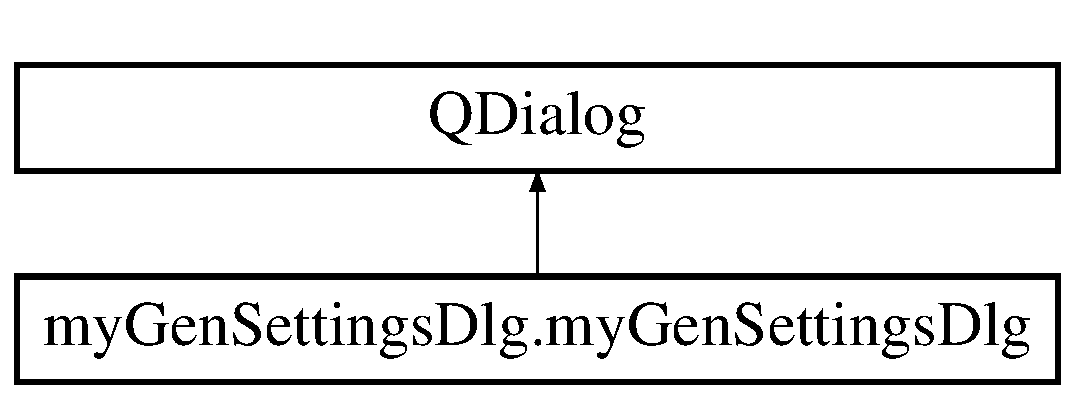
\includegraphics[height=2.000000cm]{classmy_gen_settings_dlg_1_1my_gen_settings_dlg}
\end{center}
\end{figure}
\subsection*{Public Member Functions}
\begin{DoxyCompactItemize}
\item 
def \hyperlink{classmy_gen_settings_dlg_1_1my_gen_settings_dlg_a3448925fd65dc436f29ba58f0c7e9deb}{\-\_\-\-\_\-init\-\_\-\-\_\-}
\item 
def \hyperlink{classmy_gen_settings_dlg_1_1my_gen_settings_dlg_a40a26f42e44ecf94a5b89092ab317175}{set\-Initial\-Vals}
\item 
def \hyperlink{classmy_gen_settings_dlg_1_1my_gen_settings_dlg_a5dd7698aba9583809754a31fc8238672}{make\-Str}
\item 
def \hyperlink{classmy_gen_settings_dlg_1_1my_gen_settings_dlg_a4f80cb0ec2b9ae4d4fc1ce406007d791}{get\-Vals}
\item 
def \hyperlink{classmy_gen_settings_dlg_1_1my_gen_settings_dlg_aa06ce3e18bd1fdbfc32f72ae686f4813}{set\-Arr}
\item 
def \hyperlink{classmy_gen_settings_dlg_1_1my_gen_settings_dlg_a03b1388aa3a51707339623b639675e15}{cancel\-This}
\item 
def \hyperlink{classmy_gen_settings_dlg_1_1my_gen_settings_dlg_a14c60bbaa985b6bceea42afe3fb1a44c}{close\-Up}
\end{DoxyCompactItemize}
\subsection*{Public Attributes}
\begin{DoxyCompactItemize}
\item 
\hyperlink{classmy_gen_settings_dlg_1_1my_gen_settings_dlg_a7273bd37d323cb99b1babfe474fb0794}{ui}
\item 
\hyperlink{classmy_gen_settings_dlg_1_1my_gen_settings_dlg_abb00b15bb0a18384e61e828dd8df30b7}{arr}
\item 
\hyperlink{classmy_gen_settings_dlg_1_1my_gen_settings_dlg_a0a6c727a9bd3bc9a5eccb189f58e0a6a}{status}
\end{DoxyCompactItemize}
\subsection*{Static Public Attributes}
\begin{DoxyCompactItemize}
\item 
\hyperlink{classmy_gen_settings_dlg_1_1my_gen_settings_dlg_af1f09c584de47bbe2a149f514d48bc9c}{second\-Flag} = False
\item 
string \hyperlink{classmy_gen_settings_dlg_1_1my_gen_settings_dlg_ac6e0f33c3d90c70cfb468c892557316a}{infile} = \char`\"{}\char`\"{}
\item 
int \hyperlink{classmy_gen_settings_dlg_1_1my_gen_settings_dlg_a9f34f21544d7598a99027a2d828e2c36}{status} = 0
\end{DoxyCompactItemize}


\subsection{Constructor \& Destructor Documentation}
\hypertarget{classmy_gen_settings_dlg_1_1my_gen_settings_dlg_a3448925fd65dc436f29ba58f0c7e9deb}{\index{my\-Gen\-Settings\-Dlg\-::my\-Gen\-Settings\-Dlg@{my\-Gen\-Settings\-Dlg\-::my\-Gen\-Settings\-Dlg}!\-\_\-\-\_\-init\-\_\-\-\_\-@{\-\_\-\-\_\-init\-\_\-\-\_\-}}
\index{\-\_\-\-\_\-init\-\_\-\-\_\-@{\-\_\-\-\_\-init\-\_\-\-\_\-}!myGenSettingsDlg::myGenSettingsDlg@{my\-Gen\-Settings\-Dlg\-::my\-Gen\-Settings\-Dlg}}
\subsubsection[{\-\_\-\-\_\-init\-\_\-\-\_\-}]{\setlength{\rightskip}{0pt plus 5cm}def my\-Gen\-Settings\-Dlg.\-my\-Gen\-Settings\-Dlg.\-\_\-\-\_\-init\-\_\-\-\_\- (
\begin{DoxyParamCaption}
\item[{}]{self}
\end{DoxyParamCaption}
)}}\label{classmy_gen_settings_dlg_1_1my_gen_settings_dlg_a3448925fd65dc436f29ba58f0c7e9deb}


\subsection{Member Function Documentation}
\hypertarget{classmy_gen_settings_dlg_1_1my_gen_settings_dlg_a03b1388aa3a51707339623b639675e15}{\index{my\-Gen\-Settings\-Dlg\-::my\-Gen\-Settings\-Dlg@{my\-Gen\-Settings\-Dlg\-::my\-Gen\-Settings\-Dlg}!cancel\-This@{cancel\-This}}
\index{cancel\-This@{cancel\-This}!myGenSettingsDlg::myGenSettingsDlg@{my\-Gen\-Settings\-Dlg\-::my\-Gen\-Settings\-Dlg}}
\subsubsection[{cancel\-This}]{\setlength{\rightskip}{0pt plus 5cm}def my\-Gen\-Settings\-Dlg.\-my\-Gen\-Settings\-Dlg.\-cancel\-This (
\begin{DoxyParamCaption}
\item[{}]{self}
\end{DoxyParamCaption}
)}}\label{classmy_gen_settings_dlg_1_1my_gen_settings_dlg_a03b1388aa3a51707339623b639675e15}
\hypertarget{classmy_gen_settings_dlg_1_1my_gen_settings_dlg_a14c60bbaa985b6bceea42afe3fb1a44c}{\index{my\-Gen\-Settings\-Dlg\-::my\-Gen\-Settings\-Dlg@{my\-Gen\-Settings\-Dlg\-::my\-Gen\-Settings\-Dlg}!close\-Up@{close\-Up}}
\index{close\-Up@{close\-Up}!myGenSettingsDlg::myGenSettingsDlg@{my\-Gen\-Settings\-Dlg\-::my\-Gen\-Settings\-Dlg}}
\subsubsection[{close\-Up}]{\setlength{\rightskip}{0pt plus 5cm}def my\-Gen\-Settings\-Dlg.\-my\-Gen\-Settings\-Dlg.\-close\-Up (
\begin{DoxyParamCaption}
\item[{}]{self}
\end{DoxyParamCaption}
)}}\label{classmy_gen_settings_dlg_1_1my_gen_settings_dlg_a14c60bbaa985b6bceea42afe3fb1a44c}
\hypertarget{classmy_gen_settings_dlg_1_1my_gen_settings_dlg_a4f80cb0ec2b9ae4d4fc1ce406007d791}{\index{my\-Gen\-Settings\-Dlg\-::my\-Gen\-Settings\-Dlg@{my\-Gen\-Settings\-Dlg\-::my\-Gen\-Settings\-Dlg}!get\-Vals@{get\-Vals}}
\index{get\-Vals@{get\-Vals}!myGenSettingsDlg::myGenSettingsDlg@{my\-Gen\-Settings\-Dlg\-::my\-Gen\-Settings\-Dlg}}
\subsubsection[{get\-Vals}]{\setlength{\rightskip}{0pt plus 5cm}def my\-Gen\-Settings\-Dlg.\-my\-Gen\-Settings\-Dlg.\-get\-Vals (
\begin{DoxyParamCaption}
\item[{}]{self, }
\item[{}]{array}
\end{DoxyParamCaption}
)}}\label{classmy_gen_settings_dlg_1_1my_gen_settings_dlg_a4f80cb0ec2b9ae4d4fc1ce406007d791}
\hypertarget{classmy_gen_settings_dlg_1_1my_gen_settings_dlg_a5dd7698aba9583809754a31fc8238672}{\index{my\-Gen\-Settings\-Dlg\-::my\-Gen\-Settings\-Dlg@{my\-Gen\-Settings\-Dlg\-::my\-Gen\-Settings\-Dlg}!make\-Str@{make\-Str}}
\index{make\-Str@{make\-Str}!myGenSettingsDlg::myGenSettingsDlg@{my\-Gen\-Settings\-Dlg\-::my\-Gen\-Settings\-Dlg}}
\subsubsection[{make\-Str}]{\setlength{\rightskip}{0pt plus 5cm}def my\-Gen\-Settings\-Dlg.\-my\-Gen\-Settings\-Dlg.\-make\-Str (
\begin{DoxyParamCaption}
\item[{}]{self, }
\item[{}]{num}
\end{DoxyParamCaption}
)}}\label{classmy_gen_settings_dlg_1_1my_gen_settings_dlg_a5dd7698aba9583809754a31fc8238672}
\hypertarget{classmy_gen_settings_dlg_1_1my_gen_settings_dlg_aa06ce3e18bd1fdbfc32f72ae686f4813}{\index{my\-Gen\-Settings\-Dlg\-::my\-Gen\-Settings\-Dlg@{my\-Gen\-Settings\-Dlg\-::my\-Gen\-Settings\-Dlg}!set\-Arr@{set\-Arr}}
\index{set\-Arr@{set\-Arr}!myGenSettingsDlg::myGenSettingsDlg@{my\-Gen\-Settings\-Dlg\-::my\-Gen\-Settings\-Dlg}}
\subsubsection[{set\-Arr}]{\setlength{\rightskip}{0pt plus 5cm}def my\-Gen\-Settings\-Dlg.\-my\-Gen\-Settings\-Dlg.\-set\-Arr (
\begin{DoxyParamCaption}
\item[{}]{self, }
\item[{}]{array1}
\end{DoxyParamCaption}
)}}\label{classmy_gen_settings_dlg_1_1my_gen_settings_dlg_aa06ce3e18bd1fdbfc32f72ae686f4813}
\hypertarget{classmy_gen_settings_dlg_1_1my_gen_settings_dlg_a40a26f42e44ecf94a5b89092ab317175}{\index{my\-Gen\-Settings\-Dlg\-::my\-Gen\-Settings\-Dlg@{my\-Gen\-Settings\-Dlg\-::my\-Gen\-Settings\-Dlg}!set\-Initial\-Vals@{set\-Initial\-Vals}}
\index{set\-Initial\-Vals@{set\-Initial\-Vals}!myGenSettingsDlg::myGenSettingsDlg@{my\-Gen\-Settings\-Dlg\-::my\-Gen\-Settings\-Dlg}}
\subsubsection[{set\-Initial\-Vals}]{\setlength{\rightskip}{0pt plus 5cm}def my\-Gen\-Settings\-Dlg.\-my\-Gen\-Settings\-Dlg.\-set\-Initial\-Vals (
\begin{DoxyParamCaption}
\item[{}]{self, }
\item[{}]{init\-Angle, }
\item[{}]{inc\-Angle, }
\item[{}]{start\-Number, }
\item[{}]{num\-Images, }
\item[{}]{chi, }
\item[{}]{detect, }
\item[{}]{expos\-Time}
\end{DoxyParamCaption}
)}}\label{classmy_gen_settings_dlg_1_1my_gen_settings_dlg_a40a26f42e44ecf94a5b89092ab317175}


\subsection{Member Data Documentation}
\hypertarget{classmy_gen_settings_dlg_1_1my_gen_settings_dlg_abb00b15bb0a18384e61e828dd8df30b7}{\index{my\-Gen\-Settings\-Dlg\-::my\-Gen\-Settings\-Dlg@{my\-Gen\-Settings\-Dlg\-::my\-Gen\-Settings\-Dlg}!arr@{arr}}
\index{arr@{arr}!myGenSettingsDlg::myGenSettingsDlg@{my\-Gen\-Settings\-Dlg\-::my\-Gen\-Settings\-Dlg}}
\subsubsection[{arr}]{\setlength{\rightskip}{0pt plus 5cm}my\-Gen\-Settings\-Dlg.\-my\-Gen\-Settings\-Dlg.\-arr}}\label{classmy_gen_settings_dlg_1_1my_gen_settings_dlg_abb00b15bb0a18384e61e828dd8df30b7}
\hypertarget{classmy_gen_settings_dlg_1_1my_gen_settings_dlg_ac6e0f33c3d90c70cfb468c892557316a}{\index{my\-Gen\-Settings\-Dlg\-::my\-Gen\-Settings\-Dlg@{my\-Gen\-Settings\-Dlg\-::my\-Gen\-Settings\-Dlg}!infile@{infile}}
\index{infile@{infile}!myGenSettingsDlg::myGenSettingsDlg@{my\-Gen\-Settings\-Dlg\-::my\-Gen\-Settings\-Dlg}}
\subsubsection[{infile}]{\setlength{\rightskip}{0pt plus 5cm}string my\-Gen\-Settings\-Dlg.\-my\-Gen\-Settings\-Dlg.\-infile = \char`\"{}\char`\"{}\hspace{0.3cm}{\ttfamily [static]}}}\label{classmy_gen_settings_dlg_1_1my_gen_settings_dlg_ac6e0f33c3d90c70cfb468c892557316a}
\hypertarget{classmy_gen_settings_dlg_1_1my_gen_settings_dlg_af1f09c584de47bbe2a149f514d48bc9c}{\index{my\-Gen\-Settings\-Dlg\-::my\-Gen\-Settings\-Dlg@{my\-Gen\-Settings\-Dlg\-::my\-Gen\-Settings\-Dlg}!second\-Flag@{second\-Flag}}
\index{second\-Flag@{second\-Flag}!myGenSettingsDlg::myGenSettingsDlg@{my\-Gen\-Settings\-Dlg\-::my\-Gen\-Settings\-Dlg}}
\subsubsection[{second\-Flag}]{\setlength{\rightskip}{0pt plus 5cm}my\-Gen\-Settings\-Dlg.\-my\-Gen\-Settings\-Dlg.\-second\-Flag = False\hspace{0.3cm}{\ttfamily [static]}}}\label{classmy_gen_settings_dlg_1_1my_gen_settings_dlg_af1f09c584de47bbe2a149f514d48bc9c}
\hypertarget{classmy_gen_settings_dlg_1_1my_gen_settings_dlg_a9f34f21544d7598a99027a2d828e2c36}{\index{my\-Gen\-Settings\-Dlg\-::my\-Gen\-Settings\-Dlg@{my\-Gen\-Settings\-Dlg\-::my\-Gen\-Settings\-Dlg}!status@{status}}
\index{status@{status}!myGenSettingsDlg::myGenSettingsDlg@{my\-Gen\-Settings\-Dlg\-::my\-Gen\-Settings\-Dlg}}
\subsubsection[{status}]{\setlength{\rightskip}{0pt plus 5cm}int my\-Gen\-Settings\-Dlg.\-my\-Gen\-Settings\-Dlg.\-status = 0\hspace{0.3cm}{\ttfamily [static]}}}\label{classmy_gen_settings_dlg_1_1my_gen_settings_dlg_a9f34f21544d7598a99027a2d828e2c36}
\hypertarget{classmy_gen_settings_dlg_1_1my_gen_settings_dlg_a0a6c727a9bd3bc9a5eccb189f58e0a6a}{\index{my\-Gen\-Settings\-Dlg\-::my\-Gen\-Settings\-Dlg@{my\-Gen\-Settings\-Dlg\-::my\-Gen\-Settings\-Dlg}!status@{status}}
\index{status@{status}!myGenSettingsDlg::myGenSettingsDlg@{my\-Gen\-Settings\-Dlg\-::my\-Gen\-Settings\-Dlg}}
\subsubsection[{status}]{\setlength{\rightskip}{0pt plus 5cm}my\-Gen\-Settings\-Dlg.\-my\-Gen\-Settings\-Dlg.\-status}}\label{classmy_gen_settings_dlg_1_1my_gen_settings_dlg_a0a6c727a9bd3bc9a5eccb189f58e0a6a}
\hypertarget{classmy_gen_settings_dlg_1_1my_gen_settings_dlg_a7273bd37d323cb99b1babfe474fb0794}{\index{my\-Gen\-Settings\-Dlg\-::my\-Gen\-Settings\-Dlg@{my\-Gen\-Settings\-Dlg\-::my\-Gen\-Settings\-Dlg}!ui@{ui}}
\index{ui@{ui}!myGenSettingsDlg::myGenSettingsDlg@{my\-Gen\-Settings\-Dlg\-::my\-Gen\-Settings\-Dlg}}
\subsubsection[{ui}]{\setlength{\rightskip}{0pt plus 5cm}my\-Gen\-Settings\-Dlg.\-my\-Gen\-Settings\-Dlg.\-ui}}\label{classmy_gen_settings_dlg_1_1my_gen_settings_dlg_a7273bd37d323cb99b1babfe474fb0794}


The documentation for this class was generated from the following file\-:\begin{DoxyCompactItemize}
\item 
workdir/atrex/\-Software/\hyperlink{my_gen_settings_dlg_8py}{my\-Gen\-Settings\-Dlg.\-py}\end{DoxyCompactItemize}

\hypertarget{classmy_image_1_1my_image}{\section{my\-Image.\-my\-Image Class Reference}
\label{classmy_image_1_1my_image}\index{my\-Image.\-my\-Image@{my\-Image.\-my\-Image}}
}
\subsection*{Public Member Functions}
\begin{DoxyCompactItemize}
\item 
def \hyperlink{classmy_image_1_1my_image_a204047031d17ac62cf6dc595185d4b32}{\-\_\-\-\_\-init\-\_\-\-\_\-}
\item 
def \hyperlink{classmy_image_1_1my_image_ad204cb41e7063c2c059be7edcb869fde}{read\-Tiff\-Raw}
\item 
def \hyperlink{classmy_image_1_1my_image_a9b2b7ca12028fc3c486ba1596986d200}{read\-Tiff}
\item 
def \hyperlink{classmy_image_1_1my_image_abf9d2037186dd54cfc3f98d3a14ec7b2}{read\-Text}
\item 
def \hyperlink{classmy_image_1_1my_image_a288af89bccb1aeb479746201f5f349e0}{estimate\-\_\-local\-\_\-background}
\item 
def \hyperlink{classmy_image_1_1my_image_a7d27a9c7a1708eedb66c5d2df6d83793}{grow\-\_\-peak}
\item 
def \hyperlink{classmy_image_1_1my_image_a50a355a2d27f7f62347eb2ecda76cc7f}{search\-\_\-for\-\_\-peaks\-\_\-arr}
\item 
def \hyperlink{classmy_image_1_1my_image_a947569b9e4f7e027e178961c8593e56d}{search\-\_\-for\-\_\-peaks}
\item 
def \hyperlink{classmy_image_1_1my_image_ac7d39571b3e508c285ea29391e81d83d}{apply\-Mask}
\item 
def \hyperlink{classmy_image_1_1my_image_a6d3a40f22167549a6c6d68d61c34fe88}{integrate}
\item 
def \hyperlink{classmy_image_1_1my_image_a7f239b15b61b6564c51b279b337c04a6}{cake}
\end{DoxyCompactItemize}
\subsection*{Public Attributes}
\begin{DoxyCompactItemize}
\item 
\hyperlink{classmy_image_1_1my_image_a4b84b1393353cf07c3f6a8e876b1bd1e}{Calc\-Theta}
\item 
\hyperlink{classmy_image_1_1my_image_ae621f0bcbbeb1a1c5df305d2ff74854b}{im\-File\-Name}
\item 
\hyperlink{classmy_image_1_1my_image_ae295dbccaa65f3c6d829c9f551fd1784}{im\-Array\-Size}
\item 
\hyperlink{classmy_image_1_1my_image_a3b6b9e69cb643420041fd42acfddfbb3}{im\-Array}
\item 
\hyperlink{classmy_image_1_1my_image_a906a618554e161fbe95e24b508ab6e1a}{im\-Array\-\_\-orig}
\item 
\hyperlink{classmy_image_1_1my_image_a7a46de614f68043e9420babac8f2251f}{omega0}
\item 
\hyperlink{classmy_image_1_1my_image_a48c38f81bb2ec3d332ff80510eef2846}{omega\-R}
\item 
\hyperlink{classmy_image_1_1my_image_a854752a842ba427ab11635637efd0ea5}{chi}
\item 
\hyperlink{classmy_image_1_1my_image_acb013415d500b36477f96e19ed9cc3ab}{detector}
\item 
\hyperlink{classmy_image_1_1my_image_a88013815f7b3f0a5dcd02bca7ff96b41}{exposure\-T}
\item 
\hyperlink{classmy_image_1_1my_image_a0635beb1641a5a1b7c1045dbd01bf4c4}{avg2tth}
\item 
\hyperlink{classmy_image_1_1my_image_a979ecbe45f1292ab528cefd83baad4c4}{tthetabin}
\item 
\hyperlink{classmy_image_1_1my_image_aeaf615c8bded2e97661cfc47db6d0371}{nbins\-Az}
\item 
\hyperlink{classmy_image_1_1my_image_a722eda5ce89e24cebc89da923364fb0b}{nbins\-Tth}
\item 
\hyperlink{classmy_image_1_1my_image_a5320605221fb992b852046a41947a458}{cake\-Arr}
\item 
\hyperlink{classmy_image_1_1my_image_a24f984efb2d87cb956bcce7c8a626a41}{cake\-Params}
\end{DoxyCompactItemize}
\subsection*{Static Public Attributes}
\begin{DoxyCompactItemize}
\item 
string \hyperlink{classmy_image_1_1my_image_ab9dbc690933fa5ba491388ceb1e214a0}{omega0} = ''
\item 
string \hyperlink{classmy_image_1_1my_image_ab739c7aa096b85bcdcce37dcb3c5c53c}{omega\-R} = ''
\item 
string \hyperlink{classmy_image_1_1my_image_ae0a5c8578f1aa53e8f53b522c5cf29a5}{chi} = ''
\item 
string \hyperlink{classmy_image_1_1my_image_aea69242e33fa2cc728dbfd434d44f3ed}{exposure\-T} = ''
\item 
string \hyperlink{classmy_image_1_1my_image_a0d210dc06284b429870e79968bbcbf96}{detector} = ''
\item 
list \hyperlink{classmy_image_1_1my_image_affbde3eed0befed324a6abf5d8224553}{im\-Array\-Size} = \mbox{[}0,0\mbox{]}
\item 
string \hyperlink{classmy_image_1_1my_image_a2413505e2530877553bf1c15fd5177ba}{im\-File\-Name} = ''
\end{DoxyCompactItemize}


\subsection{Constructor \& Destructor Documentation}
\hypertarget{classmy_image_1_1my_image_a204047031d17ac62cf6dc595185d4b32}{\index{my\-Image\-::my\-Image@{my\-Image\-::my\-Image}!\-\_\-\-\_\-init\-\_\-\-\_\-@{\-\_\-\-\_\-init\-\_\-\-\_\-}}
\index{\-\_\-\-\_\-init\-\_\-\-\_\-@{\-\_\-\-\_\-init\-\_\-\-\_\-}!myImage::myImage@{my\-Image\-::my\-Image}}
\subsubsection[{\-\_\-\-\_\-init\-\_\-\-\_\-}]{\setlength{\rightskip}{0pt plus 5cm}def my\-Image.\-my\-Image.\-\_\-\-\_\-init\-\_\-\-\_\- (
\begin{DoxyParamCaption}
\item[{}]{self}
\end{DoxyParamCaption}
)}}\label{classmy_image_1_1my_image_a204047031d17ac62cf6dc595185d4b32}


\subsection{Member Function Documentation}
\hypertarget{classmy_image_1_1my_image_ac7d39571b3e508c285ea29391e81d83d}{\index{my\-Image\-::my\-Image@{my\-Image\-::my\-Image}!apply\-Mask@{apply\-Mask}}
\index{apply\-Mask@{apply\-Mask}!myImage::myImage@{my\-Image\-::my\-Image}}
\subsubsection[{apply\-Mask}]{\setlength{\rightskip}{0pt plus 5cm}def my\-Image.\-my\-Image.\-apply\-Mask (
\begin{DoxyParamCaption}
\item[{}]{self, }
\item[{}]{arr}
\end{DoxyParamCaption}
)}}\label{classmy_image_1_1my_image_ac7d39571b3e508c285ea29391e81d83d}
\hypertarget{classmy_image_1_1my_image_a7f239b15b61b6564c51b279b337c04a6}{\index{my\-Image\-::my\-Image@{my\-Image\-::my\-Image}!cake@{cake}}
\index{cake@{cake}!myImage::myImage@{my\-Image\-::my\-Image}}
\subsubsection[{cake}]{\setlength{\rightskip}{0pt plus 5cm}def my\-Image.\-my\-Image.\-cake (
\begin{DoxyParamCaption}
\item[{}]{self, }
\item[{}]{beam, }
\item[{}]{ttheta\-Arr}
\end{DoxyParamCaption}
)}}\label{classmy_image_1_1my_image_a7f239b15b61b6564c51b279b337c04a6}
\hypertarget{classmy_image_1_1my_image_a288af89bccb1aeb479746201f5f349e0}{\index{my\-Image\-::my\-Image@{my\-Image\-::my\-Image}!estimate\-\_\-local\-\_\-background@{estimate\-\_\-local\-\_\-background}}
\index{estimate\-\_\-local\-\_\-background@{estimate\-\_\-local\-\_\-background}!myImage::myImage@{my\-Image\-::my\-Image}}
\subsubsection[{estimate\-\_\-local\-\_\-background}]{\setlength{\rightskip}{0pt plus 5cm}def my\-Image.\-my\-Image.\-estimate\-\_\-local\-\_\-background (
\begin{DoxyParamCaption}
\item[{}]{self, }
\item[{}]{img, }
\item[{}]{nbinx, }
\item[{}]{nbiny, }
\item[{}]{thr, }
\item[{}]{perc}
\end{DoxyParamCaption}
)}}\label{classmy_image_1_1my_image_a288af89bccb1aeb479746201f5f349e0}
\hypertarget{classmy_image_1_1my_image_a7d27a9c7a1708eedb66c5d2df6d83793}{\index{my\-Image\-::my\-Image@{my\-Image\-::my\-Image}!grow\-\_\-peak@{grow\-\_\-peak}}
\index{grow\-\_\-peak@{grow\-\_\-peak}!myImage::myImage@{my\-Image\-::my\-Image}}
\subsubsection[{grow\-\_\-peak}]{\setlength{\rightskip}{0pt plus 5cm}def my\-Image.\-my\-Image.\-grow\-\_\-peak (
\begin{DoxyParamCaption}
\item[{}]{self, }
\item[{}]{arr, }
\item[{}]{bkg, }
\item[{}]{x, }
\item[{}]{y, }
\item[{}]{mins, }
\item[{}]{xmax, }
\item[{}]{ymax}
\end{DoxyParamCaption}
)}}\label{classmy_image_1_1my_image_a7d27a9c7a1708eedb66c5d2df6d83793}
\hypertarget{classmy_image_1_1my_image_a6d3a40f22167549a6c6d68d61c34fe88}{\index{my\-Image\-::my\-Image@{my\-Image\-::my\-Image}!integrate@{integrate}}
\index{integrate@{integrate}!myImage::myImage@{my\-Image\-::my\-Image}}
\subsubsection[{integrate}]{\setlength{\rightskip}{0pt plus 5cm}def my\-Image.\-my\-Image.\-integrate (
\begin{DoxyParamCaption}
\item[{}]{self, }
\item[{}]{beam, }
\item[{}]{ttheta\-Arr}
\end{DoxyParamCaption}
)}}\label{classmy_image_1_1my_image_a6d3a40f22167549a6c6d68d61c34fe88}
\hypertarget{classmy_image_1_1my_image_abf9d2037186dd54cfc3f98d3a14ec7b2}{\index{my\-Image\-::my\-Image@{my\-Image\-::my\-Image}!read\-Text@{read\-Text}}
\index{read\-Text@{read\-Text}!myImage::myImage@{my\-Image\-::my\-Image}}
\subsubsection[{read\-Text}]{\setlength{\rightskip}{0pt plus 5cm}def my\-Image.\-my\-Image.\-read\-Text (
\begin{DoxyParamCaption}
\item[{}]{self, }
\item[{}]{infile}
\end{DoxyParamCaption}
)}}\label{classmy_image_1_1my_image_abf9d2037186dd54cfc3f98d3a14ec7b2}
\hypertarget{classmy_image_1_1my_image_a9b2b7ca12028fc3c486ba1596986d200}{\index{my\-Image\-::my\-Image@{my\-Image\-::my\-Image}!read\-Tiff@{read\-Tiff}}
\index{read\-Tiff@{read\-Tiff}!myImage::myImage@{my\-Image\-::my\-Image}}
\subsubsection[{read\-Tiff}]{\setlength{\rightskip}{0pt plus 5cm}def my\-Image.\-my\-Image.\-read\-Tiff (
\begin{DoxyParamCaption}
\item[{}]{self, }
\item[{}]{infile}
\end{DoxyParamCaption}
)}}\label{classmy_image_1_1my_image_a9b2b7ca12028fc3c486ba1596986d200}
\hypertarget{classmy_image_1_1my_image_ad204cb41e7063c2c059be7edcb869fde}{\index{my\-Image\-::my\-Image@{my\-Image\-::my\-Image}!read\-Tiff\-Raw@{read\-Tiff\-Raw}}
\index{read\-Tiff\-Raw@{read\-Tiff\-Raw}!myImage::myImage@{my\-Image\-::my\-Image}}
\subsubsection[{read\-Tiff\-Raw}]{\setlength{\rightskip}{0pt plus 5cm}def my\-Image.\-my\-Image.\-read\-Tiff\-Raw (
\begin{DoxyParamCaption}
\item[{}]{self, }
\item[{}]{infile}
\end{DoxyParamCaption}
)}}\label{classmy_image_1_1my_image_ad204cb41e7063c2c059be7edcb869fde}
\hypertarget{classmy_image_1_1my_image_a947569b9e4f7e027e178961c8593e56d}{\index{my\-Image\-::my\-Image@{my\-Image\-::my\-Image}!search\-\_\-for\-\_\-peaks@{search\-\_\-for\-\_\-peaks}}
\index{search\-\_\-for\-\_\-peaks@{search\-\_\-for\-\_\-peaks}!myImage::myImage@{my\-Image\-::my\-Image}}
\subsubsection[{search\-\_\-for\-\_\-peaks}]{\setlength{\rightskip}{0pt plus 5cm}def my\-Image.\-my\-Image.\-search\-\_\-for\-\_\-peaks (
\begin{DoxyParamCaption}
\item[{}]{self, }
\item[{}]{peaks, }
\item[{}]{thr, }
\item[{}]{max\-\_\-peak\-\_\-size, }
\item[{}]{num\-\_\-of\-\_\-segments, }
\item[{}]{perc}
\end{DoxyParamCaption}
)}}\label{classmy_image_1_1my_image_a947569b9e4f7e027e178961c8593e56d}
\hypertarget{classmy_image_1_1my_image_a50a355a2d27f7f62347eb2ecda76cc7f}{\index{my\-Image\-::my\-Image@{my\-Image\-::my\-Image}!search\-\_\-for\-\_\-peaks\-\_\-arr@{search\-\_\-for\-\_\-peaks\-\_\-arr}}
\index{search\-\_\-for\-\_\-peaks\-\_\-arr@{search\-\_\-for\-\_\-peaks\-\_\-arr}!myImage::myImage@{my\-Image\-::my\-Image}}
\subsubsection[{search\-\_\-for\-\_\-peaks\-\_\-arr}]{\setlength{\rightskip}{0pt plus 5cm}def my\-Image.\-my\-Image.\-search\-\_\-for\-\_\-peaks\-\_\-arr (
\begin{DoxyParamCaption}
\item[{}]{self, }
\item[{}]{arr, }
\item[{}]{peaks, }
\item[{}]{thr, }
\item[{}]{max\-\_\-peak\-\_\-size, }
\item[{}]{num\-\_\-of\-\_\-segments, }
\item[{}]{perc}
\end{DoxyParamCaption}
)}}\label{classmy_image_1_1my_image_a50a355a2d27f7f62347eb2ecda76cc7f}


\subsection{Member Data Documentation}
\hypertarget{classmy_image_1_1my_image_a0635beb1641a5a1b7c1045dbd01bf4c4}{\index{my\-Image\-::my\-Image@{my\-Image\-::my\-Image}!avg2tth@{avg2tth}}
\index{avg2tth@{avg2tth}!myImage::myImage@{my\-Image\-::my\-Image}}
\subsubsection[{avg2tth}]{\setlength{\rightskip}{0pt plus 5cm}my\-Image.\-my\-Image.\-avg2tth}}\label{classmy_image_1_1my_image_a0635beb1641a5a1b7c1045dbd01bf4c4}
\hypertarget{classmy_image_1_1my_image_a5320605221fb992b852046a41947a458}{\index{my\-Image\-::my\-Image@{my\-Image\-::my\-Image}!cake\-Arr@{cake\-Arr}}
\index{cake\-Arr@{cake\-Arr}!myImage::myImage@{my\-Image\-::my\-Image}}
\subsubsection[{cake\-Arr}]{\setlength{\rightskip}{0pt plus 5cm}my\-Image.\-my\-Image.\-cake\-Arr}}\label{classmy_image_1_1my_image_a5320605221fb992b852046a41947a458}
\hypertarget{classmy_image_1_1my_image_a24f984efb2d87cb956bcce7c8a626a41}{\index{my\-Image\-::my\-Image@{my\-Image\-::my\-Image}!cake\-Params@{cake\-Params}}
\index{cake\-Params@{cake\-Params}!myImage::myImage@{my\-Image\-::my\-Image}}
\subsubsection[{cake\-Params}]{\setlength{\rightskip}{0pt plus 5cm}my\-Image.\-my\-Image.\-cake\-Params}}\label{classmy_image_1_1my_image_a24f984efb2d87cb956bcce7c8a626a41}
\hypertarget{classmy_image_1_1my_image_a4b84b1393353cf07c3f6a8e876b1bd1e}{\index{my\-Image\-::my\-Image@{my\-Image\-::my\-Image}!Calc\-Theta@{Calc\-Theta}}
\index{Calc\-Theta@{Calc\-Theta}!myImage::myImage@{my\-Image\-::my\-Image}}
\subsubsection[{Calc\-Theta}]{\setlength{\rightskip}{0pt plus 5cm}my\-Image.\-my\-Image.\-Calc\-Theta}}\label{classmy_image_1_1my_image_a4b84b1393353cf07c3f6a8e876b1bd1e}
\hypertarget{classmy_image_1_1my_image_ae0a5c8578f1aa53e8f53b522c5cf29a5}{\index{my\-Image\-::my\-Image@{my\-Image\-::my\-Image}!chi@{chi}}
\index{chi@{chi}!myImage::myImage@{my\-Image\-::my\-Image}}
\subsubsection[{chi}]{\setlength{\rightskip}{0pt plus 5cm}string my\-Image.\-my\-Image.\-chi = ''\hspace{0.3cm}{\ttfamily [static]}}}\label{classmy_image_1_1my_image_ae0a5c8578f1aa53e8f53b522c5cf29a5}
\hypertarget{classmy_image_1_1my_image_a854752a842ba427ab11635637efd0ea5}{\index{my\-Image\-::my\-Image@{my\-Image\-::my\-Image}!chi@{chi}}
\index{chi@{chi}!myImage::myImage@{my\-Image\-::my\-Image}}
\subsubsection[{chi}]{\setlength{\rightskip}{0pt plus 5cm}my\-Image.\-my\-Image.\-chi}}\label{classmy_image_1_1my_image_a854752a842ba427ab11635637efd0ea5}
\hypertarget{classmy_image_1_1my_image_a0d210dc06284b429870e79968bbcbf96}{\index{my\-Image\-::my\-Image@{my\-Image\-::my\-Image}!detector@{detector}}
\index{detector@{detector}!myImage::myImage@{my\-Image\-::my\-Image}}
\subsubsection[{detector}]{\setlength{\rightskip}{0pt plus 5cm}string my\-Image.\-my\-Image.\-detector = ''\hspace{0.3cm}{\ttfamily [static]}}}\label{classmy_image_1_1my_image_a0d210dc06284b429870e79968bbcbf96}
\hypertarget{classmy_image_1_1my_image_acb013415d500b36477f96e19ed9cc3ab}{\index{my\-Image\-::my\-Image@{my\-Image\-::my\-Image}!detector@{detector}}
\index{detector@{detector}!myImage::myImage@{my\-Image\-::my\-Image}}
\subsubsection[{detector}]{\setlength{\rightskip}{0pt plus 5cm}my\-Image.\-my\-Image.\-detector}}\label{classmy_image_1_1my_image_acb013415d500b36477f96e19ed9cc3ab}
\hypertarget{classmy_image_1_1my_image_aea69242e33fa2cc728dbfd434d44f3ed}{\index{my\-Image\-::my\-Image@{my\-Image\-::my\-Image}!exposure\-T@{exposure\-T}}
\index{exposure\-T@{exposure\-T}!myImage::myImage@{my\-Image\-::my\-Image}}
\subsubsection[{exposure\-T}]{\setlength{\rightskip}{0pt plus 5cm}string my\-Image.\-my\-Image.\-exposure\-T = ''\hspace{0.3cm}{\ttfamily [static]}}}\label{classmy_image_1_1my_image_aea69242e33fa2cc728dbfd434d44f3ed}
\hypertarget{classmy_image_1_1my_image_a88013815f7b3f0a5dcd02bca7ff96b41}{\index{my\-Image\-::my\-Image@{my\-Image\-::my\-Image}!exposure\-T@{exposure\-T}}
\index{exposure\-T@{exposure\-T}!myImage::myImage@{my\-Image\-::my\-Image}}
\subsubsection[{exposure\-T}]{\setlength{\rightskip}{0pt plus 5cm}my\-Image.\-my\-Image.\-exposure\-T}}\label{classmy_image_1_1my_image_a88013815f7b3f0a5dcd02bca7ff96b41}
\hypertarget{classmy_image_1_1my_image_a3b6b9e69cb643420041fd42acfddfbb3}{\index{my\-Image\-::my\-Image@{my\-Image\-::my\-Image}!im\-Array@{im\-Array}}
\index{im\-Array@{im\-Array}!myImage::myImage@{my\-Image\-::my\-Image}}
\subsubsection[{im\-Array}]{\setlength{\rightskip}{0pt plus 5cm}my\-Image.\-my\-Image.\-im\-Array}}\label{classmy_image_1_1my_image_a3b6b9e69cb643420041fd42acfddfbb3}
\hypertarget{classmy_image_1_1my_image_a906a618554e161fbe95e24b508ab6e1a}{\index{my\-Image\-::my\-Image@{my\-Image\-::my\-Image}!im\-Array\-\_\-orig@{im\-Array\-\_\-orig}}
\index{im\-Array\-\_\-orig@{im\-Array\-\_\-orig}!myImage::myImage@{my\-Image\-::my\-Image}}
\subsubsection[{im\-Array\-\_\-orig}]{\setlength{\rightskip}{0pt plus 5cm}my\-Image.\-my\-Image.\-im\-Array\-\_\-orig}}\label{classmy_image_1_1my_image_a906a618554e161fbe95e24b508ab6e1a}
\hypertarget{classmy_image_1_1my_image_affbde3eed0befed324a6abf5d8224553}{\index{my\-Image\-::my\-Image@{my\-Image\-::my\-Image}!im\-Array\-Size@{im\-Array\-Size}}
\index{im\-Array\-Size@{im\-Array\-Size}!myImage::myImage@{my\-Image\-::my\-Image}}
\subsubsection[{im\-Array\-Size}]{\setlength{\rightskip}{0pt plus 5cm}list my\-Image.\-my\-Image.\-im\-Array\-Size = \mbox{[}0,0\mbox{]}\hspace{0.3cm}{\ttfamily [static]}}}\label{classmy_image_1_1my_image_affbde3eed0befed324a6abf5d8224553}
\hypertarget{classmy_image_1_1my_image_ae295dbccaa65f3c6d829c9f551fd1784}{\index{my\-Image\-::my\-Image@{my\-Image\-::my\-Image}!im\-Array\-Size@{im\-Array\-Size}}
\index{im\-Array\-Size@{im\-Array\-Size}!myImage::myImage@{my\-Image\-::my\-Image}}
\subsubsection[{im\-Array\-Size}]{\setlength{\rightskip}{0pt plus 5cm}my\-Image.\-my\-Image.\-im\-Array\-Size}}\label{classmy_image_1_1my_image_ae295dbccaa65f3c6d829c9f551fd1784}
\hypertarget{classmy_image_1_1my_image_a2413505e2530877553bf1c15fd5177ba}{\index{my\-Image\-::my\-Image@{my\-Image\-::my\-Image}!im\-File\-Name@{im\-File\-Name}}
\index{im\-File\-Name@{im\-File\-Name}!myImage::myImage@{my\-Image\-::my\-Image}}
\subsubsection[{im\-File\-Name}]{\setlength{\rightskip}{0pt plus 5cm}string my\-Image.\-my\-Image.\-im\-File\-Name = ''\hspace{0.3cm}{\ttfamily [static]}}}\label{classmy_image_1_1my_image_a2413505e2530877553bf1c15fd5177ba}
\hypertarget{classmy_image_1_1my_image_ae621f0bcbbeb1a1c5df305d2ff74854b}{\index{my\-Image\-::my\-Image@{my\-Image\-::my\-Image}!im\-File\-Name@{im\-File\-Name}}
\index{im\-File\-Name@{im\-File\-Name}!myImage::myImage@{my\-Image\-::my\-Image}}
\subsubsection[{im\-File\-Name}]{\setlength{\rightskip}{0pt plus 5cm}my\-Image.\-my\-Image.\-im\-File\-Name}}\label{classmy_image_1_1my_image_ae621f0bcbbeb1a1c5df305d2ff74854b}
\hypertarget{classmy_image_1_1my_image_aeaf615c8bded2e97661cfc47db6d0371}{\index{my\-Image\-::my\-Image@{my\-Image\-::my\-Image}!nbins\-Az@{nbins\-Az}}
\index{nbins\-Az@{nbins\-Az}!myImage::myImage@{my\-Image\-::my\-Image}}
\subsubsection[{nbins\-Az}]{\setlength{\rightskip}{0pt plus 5cm}my\-Image.\-my\-Image.\-nbins\-Az}}\label{classmy_image_1_1my_image_aeaf615c8bded2e97661cfc47db6d0371}
\hypertarget{classmy_image_1_1my_image_a722eda5ce89e24cebc89da923364fb0b}{\index{my\-Image\-::my\-Image@{my\-Image\-::my\-Image}!nbins\-Tth@{nbins\-Tth}}
\index{nbins\-Tth@{nbins\-Tth}!myImage::myImage@{my\-Image\-::my\-Image}}
\subsubsection[{nbins\-Tth}]{\setlength{\rightskip}{0pt plus 5cm}my\-Image.\-my\-Image.\-nbins\-Tth}}\label{classmy_image_1_1my_image_a722eda5ce89e24cebc89da923364fb0b}
\hypertarget{classmy_image_1_1my_image_ab9dbc690933fa5ba491388ceb1e214a0}{\index{my\-Image\-::my\-Image@{my\-Image\-::my\-Image}!omega0@{omega0}}
\index{omega0@{omega0}!myImage::myImage@{my\-Image\-::my\-Image}}
\subsubsection[{omega0}]{\setlength{\rightskip}{0pt plus 5cm}string my\-Image.\-my\-Image.\-omega0 = ''\hspace{0.3cm}{\ttfamily [static]}}}\label{classmy_image_1_1my_image_ab9dbc690933fa5ba491388ceb1e214a0}
\hypertarget{classmy_image_1_1my_image_a7a46de614f68043e9420babac8f2251f}{\index{my\-Image\-::my\-Image@{my\-Image\-::my\-Image}!omega0@{omega0}}
\index{omega0@{omega0}!myImage::myImage@{my\-Image\-::my\-Image}}
\subsubsection[{omega0}]{\setlength{\rightskip}{0pt plus 5cm}my\-Image.\-my\-Image.\-omega0}}\label{classmy_image_1_1my_image_a7a46de614f68043e9420babac8f2251f}
\hypertarget{classmy_image_1_1my_image_ab739c7aa096b85bcdcce37dcb3c5c53c}{\index{my\-Image\-::my\-Image@{my\-Image\-::my\-Image}!omega\-R@{omega\-R}}
\index{omega\-R@{omega\-R}!myImage::myImage@{my\-Image\-::my\-Image}}
\subsubsection[{omega\-R}]{\setlength{\rightskip}{0pt plus 5cm}string my\-Image.\-my\-Image.\-omega\-R = ''\hspace{0.3cm}{\ttfamily [static]}}}\label{classmy_image_1_1my_image_ab739c7aa096b85bcdcce37dcb3c5c53c}
\hypertarget{classmy_image_1_1my_image_a48c38f81bb2ec3d332ff80510eef2846}{\index{my\-Image\-::my\-Image@{my\-Image\-::my\-Image}!omega\-R@{omega\-R}}
\index{omega\-R@{omega\-R}!myImage::myImage@{my\-Image\-::my\-Image}}
\subsubsection[{omega\-R}]{\setlength{\rightskip}{0pt plus 5cm}my\-Image.\-my\-Image.\-omega\-R}}\label{classmy_image_1_1my_image_a48c38f81bb2ec3d332ff80510eef2846}
\hypertarget{classmy_image_1_1my_image_a979ecbe45f1292ab528cefd83baad4c4}{\index{my\-Image\-::my\-Image@{my\-Image\-::my\-Image}!tthetabin@{tthetabin}}
\index{tthetabin@{tthetabin}!myImage::myImage@{my\-Image\-::my\-Image}}
\subsubsection[{tthetabin}]{\setlength{\rightskip}{0pt plus 5cm}my\-Image.\-my\-Image.\-tthetabin}}\label{classmy_image_1_1my_image_a979ecbe45f1292ab528cefd83baad4c4}


The documentation for this class was generated from the following file\-:\begin{DoxyCompactItemize}
\item 
workdir/atrex/\-Software/\hyperlink{my_image_8py}{my\-Image.\-py}\end{DoxyCompactItemize}

\hypertarget{classmy_im_display_1_1my_im_display}{\section{my\-Im\-Display.\-my\-Im\-Display Class Reference}
\label{classmy_im_display_1_1my_im_display}\index{my\-Im\-Display.\-my\-Im\-Display@{my\-Im\-Display.\-my\-Im\-Display}}
}
Inheritance diagram for my\-Im\-Display.\-my\-Im\-Display\-:\begin{figure}[H]
\begin{center}
\leavevmode
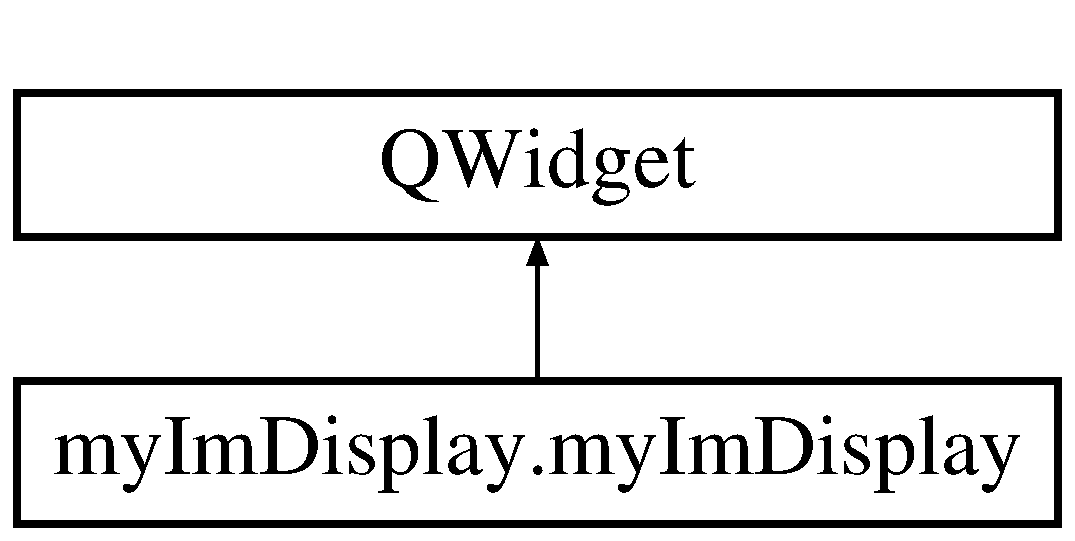
\includegraphics[height=2.000000cm]{classmy_im_display_1_1my_im_display}
\end{center}
\end{figure}
\subsection*{Public Member Functions}
\begin{DoxyCompactItemize}
\item 
def \hyperlink{classmy_im_display_1_1my_im_display_ac84ff467e290df4e4ab1d4c65d4267f5}{\-\_\-\-\_\-init\-\_\-\-\_\-}
\item 
def \hyperlink{classmy_im_display_1_1my_im_display_ab744180f478698e143f8470430f1d192}{set\-Peak\-Box\-Size}
\item 
def \hyperlink{classmy_im_display_1_1my_im_display_ab09a20ba11a398d503273b7f422c2644}{set\-Cake\-Image}
\item 
def \hyperlink{classmy_im_display_1_1my_im_display_a3352c4bc953e0a9f393d08871e5d1c31}{context\-Menu\-Kickoff}
\item 
def \hyperlink{classmy_im_display_1_1my_im_display_a8093fb201222b74f57c27297f1e6d84a}{zoom\-On}
\item 
def \hyperlink{classmy_im_display_1_1my_im_display_ae60543e0ec298c4a15e385f11091b675}{peak\-Add}
\item 
def \hyperlink{classmy_im_display_1_1my_im_display_a29d16cbb8188fd3f8c15fa6014b231e8}{select\-On}
\item 
def \hyperlink{classmy_im_display_1_1my_im_display_a6f9207ced879b40fb101f1994ba71eef}{unselect\-On}
\item 
def \hyperlink{classmy_im_display_1_1my_im_display_a7411fd0ab99914cd633c779309de1d07}{mask\-On}
\item 
def \hyperlink{classmy_im_display_1_1my_im_display_a30939cb6a115426fc1d37960cbb19297}{unmask\-On}
\item 
def \hyperlink{classmy_im_display_1_1my_im_display_acd33a2cd440fea030b809b07d9356e10}{set\-Min\-Max}
\item 
def \hyperlink{classmy_im_display_1_1my_im_display_a68c47131be6412075f42b0b1725f9964}{set\-Zm\-Rect}
\item 
def \hyperlink{classmy_im_display_1_1my_im_display_a05a3f0227ee151a60323a4c1a98fb48f}{calc\-Histo}
\item 
def \hyperlink{classmy_im_display_1_1my_im_display_a54c41ffb58933e7d11d44267fd893330}{write\-Q\-Image}
\item 
def \hyperlink{classmy_im_display_1_1my_im_display_aaf7a8e0381472923f2b0c40ab8b2b842}{write\-Q\-Image\-\_\-lut}
\item 
def \hyperlink{classmy_im_display_1_1my_im_display_a4547adad958556b811c45e2a4b89308e}{set\-L\-U\-T}
\item 
def \hyperlink{classmy_im_display_1_1my_im_display_a5085f34b80cfdd3b00758515585a0fbf}{mouse\-Release\-Event}
\begin{DoxyCompactList}\small\item\em Mouse Functions. \end{DoxyCompactList}\item 
def \hyperlink{classmy_im_display_1_1my_im_display_aff9f38dbac669da47bfb829837b8b74b}{mouse\-Press\-Event}
\item 
def \hyperlink{classmy_im_display_1_1my_im_display_ac65f590d7f74cf11fc8dcb2dfa3eb669}{mouse\-Move\-Event}
\item 
def \hyperlink{classmy_im_display_1_1my_im_display_a5ef52021cb9f418ed66ef0d8ba064430}{peak\-Find}
\item 
def \hyperlink{classmy_im_display_1_1my_im_display_a4408bd12e5abc5fb4f6e82bec3bb22c8}{set\-Peaks}
\item 
def \hyperlink{classmy_im_display_1_1my_im_display_a4c809a5912d974d2d819b5b1937638cd}{paint\-Event}
\item 
def \hyperlink{classmy_im_display_1_1my_im_display_a6bb6690d1ba6d5087ca3520d7095a625}{apply\-Mask}
\item 
def \hyperlink{classmy_im_display_1_1my_im_display_ab0ad3b819095b75f6f02df31428d7e03}{apply\-Mask\-To\-Array}
\item 
def \hyperlink{classmy_im_display_1_1my_im_display_a9dbb51a8119e4699a1fa0fd757bb1e09}{set\-Calibration\-Marks}
\item 
def \hyperlink{classmy_im_display_1_1my_im_display_ab0ad940e09349167e907fccb728efbe0}{set\-Prox\-Points}
\end{DoxyCompactItemize}
\subsection*{Public Attributes}
\begin{DoxyCompactItemize}
\item 
\hyperlink{classmy_im_display_1_1my_im_display_a388bff72546f1d6fac13520142b77095}{cal\-Points\-Flag}
\item 
\hyperlink{classmy_im_display_1_1my_im_display_ae2050cee691f881f69d1bc9caa02b8f5}{cal\-Points}
\item 
\hyperlink{classmy_im_display_1_1my_im_display_acc86c3f609b093d1dab093d5d458db1c}{prox\-Points}
\item 
\hyperlink{classmy_im_display_1_1my_im_display_aa0bc29d37aa4ceea5a1b6e73bb1b5b2a}{prox\-Points\-F}
\item 
\hyperlink{classmy_im_display_1_1my_im_display_abe157e3a38400a86b33ed3ad78aee75d}{peak\-Box\-Size}
\item 
\hyperlink{classmy_im_display_1_1my_im_display_a73cfa3418c302cd63b7583b44b9c3b98}{disp\-Min}
\item 
\hyperlink{classmy_im_display_1_1my_im_display_a9472fc9988a7d5b4b3d26555eff36629}{disp\-Max}
\item 
\hyperlink{classmy_im_display_1_1my_im_display_a2fef2a841184ea3d06026f30fedb9c68}{zm\-Rect}
\item 
\hyperlink{classmy_im_display_1_1my_im_display_ad52cc4c765b66c9200b3d3fbf8415170}{zm\-Size}
\item 
\hyperlink{classmy_im_display_1_1my_im_display_a6ae8912d4d04b0a655e1a01fd8070ff6}{ind\-\_\-5}
\item 
\hyperlink{classmy_im_display_1_1my_im_display_a4d83de595869c13b63e303709bc188a7}{ind\-\_\-95}
\item 
\hyperlink{classmy_im_display_1_1my_im_display_a781283f5accbbaf7562ef6c4a85b662c}{xsize}
\item 
\hyperlink{classmy_im_display_1_1my_im_display_acd126c9a2504bff9bc339acc8f4160d4}{ysize}
\item 
\hyperlink{classmy_im_display_1_1my_im_display_ad82dd773b3509d7c4d283654bc2b22fe}{fulldata}
\item 
\hyperlink{classmy_im_display_1_1my_im_display_a3643bcc46e320625be4b0a16a366398b}{max}
\item 
\hyperlink{classmy_im_display_1_1my_im_display_a44e480bf21d1b2f540d95b03d0e41678}{min}
\item 
\hyperlink{classmy_im_display_1_1my_im_display_a60a3651bd482b77f17fd9758418576a6}{scale}
\item 
\hyperlink{classmy_im_display_1_1my_im_display_a0a4c2d42cb88a1ffcc46de46f97298df}{pscale}
\item 
\hyperlink{classmy_im_display_1_1my_im_display_a4aaf1f57b9b82bc1fc8baa8bbb178222}{qimage}
\item 
\hyperlink{classmy_im_display_1_1my_im_display_a9746a399ab1bed5e1dd795f5996cc242}{load\-Image}
\item 
\hyperlink{classmy_im_display_1_1my_im_display_a9aca945926bdc3f037ba0cc3b155b1a8}{zm\-Fac}
\item 
\hyperlink{classmy_im_display_1_1my_im_display_a9e8a54943407a7cce248d03f5b62741a}{imdata}
\item 
\hyperlink{classmy_im_display_1_1my_im_display_aa82904a08c5b57df3520dfb0496ce1ba}{rgb\-\_\-lut}
\item 
\hyperlink{classmy_im_display_1_1my_im_display_aa8be69b012304960b810c37fc9212abb}{select\-Point\-U\-L}
\item 
\hyperlink{classmy_im_display_1_1my_im_display_a520d206f02a9731fb993705899044d46}{select\-Point\-L\-R}
\item 
\hyperlink{classmy_im_display_1_1my_im_display_af40bf78fd8315226eedca459d686ca05}{dmax}
\item 
\hyperlink{classmy_im_display_1_1my_im_display_aead7802bb20d7a0d6d7f6f680b1cb7e2}{peaks}
\item 
\hyperlink{classmy_im_display_1_1my_im_display_afde0c76a92daa96ba2d868fe4ee9a228}{curmask}
\end{DoxyCompactItemize}
\subsection*{Static Public Attributes}
\begin{DoxyCompactItemize}
\item 
int \hyperlink{classmy_im_display_1_1my_im_display_aeaa8491db62f6e99ba83f6fa81dc6d74}{load\-Image} = 0
\item 
int \hyperlink{classmy_im_display_1_1my_im_display_aaff409ee4de877ac2f0fcb090e1a5daf}{disp\-Max} = 65535
\item 
int \hyperlink{classmy_im_display_1_1my_im_display_a795083e40d9aa9b6e7d4a5d37910e187}{disp\-Min} = 0
\item 
int \hyperlink{classmy_im_display_1_1my_im_display_a4c5cc84a1c8d090c4c43d8f78b7b4d9f}{ind\-\_\-5} = 0
\item 
int \hyperlink{classmy_im_display_1_1my_im_display_a34f600eea208832c0b785288ccad9fc7}{zm\-Fac} = 3
\item 
tuple \hyperlink{classmy_im_display_1_1my_im_display_a02f7742e2c4e540f6585f39c8af717cb}{zm\-Rect} = Qt\-Core.\-Q\-Rect()
\item 
tuple \hyperlink{classmy_im_display_1_1my_im_display_afe92f10aebabc4ab5d3f18a6fea84d75}{cent\-Pt} = Qt\-Core.\-pyqt\-Signal(Qt\-Core.\-Q\-Point)
\item 
tuple \hyperlink{classmy_im_display_1_1my_im_display_a52347d8a98f02a25ddc2929a08461909}{add\-Peak\-Signal} = Qt\-Core.\-pyqt\-Signal(Qt\-Core.\-Q\-Point)
\item 
tuple \hyperlink{classmy_im_display_1_1my_im_display_a9e0436ef995b6fa9769ab1cc004956e4}{select\-Rect\-Signal} = Qt\-Core.\-pyqt\-Signal(Qt\-Core.\-Q\-Rect, bool)
\item 
tuple \hyperlink{classmy_im_display_1_1my_im_display_aebd7f068977c74a612f0428fe26bf86c}{mask\-Rect\-Signal} = Qt\-Core.\-pyqt\-Signal(Qt\-Core.\-Q\-Rect, bool)
\item 
tuple \hyperlink{classmy_im_display_1_1my_im_display_a4c70f21c598d0b670373d09133d09767}{set\-Button\-Mode\-Signal} = Qt\-Core.\-pyqt\-Signal(int)
\item 
tuple \hyperlink{classmy_im_display_1_1my_im_display_a1f5a4286181533164cb3ab70ee622264}{imcoords\-Select\-Signal} = Qt\-Core.\-pyqt\-Signal(list)
\item 
\hyperlink{classmy_im_display_1_1my_im_display_aed334f8955978445c19ec065984ffdf1}{drag\-Zm} = False
\item 
\hyperlink{classmy_im_display_1_1my_im_display_a1ede5c771d24ccc9bc28d13b9af5aea9}{zoom\-Toggle} = True
\item 
\hyperlink{classmy_im_display_1_1my_im_display_a14cb30b4564e4b042b23f20adbf38c72}{peak\-Toggle} = False
\item 
\hyperlink{classmy_im_display_1_1my_im_display_a233a9c327101136d4cf81d5e47f22f08}{select\-Flag} = False
\item 
\hyperlink{classmy_im_display_1_1my_im_display_a31a7d969ae2427fdc98ac41f7097ba5a}{unselect\-Flag} = False
\item 
\hyperlink{classmy_im_display_1_1my_im_display_a1afbe7e34027cf61cd59d25b90de33e4}{mask\-Flag} = False
\item 
\hyperlink{classmy_im_display_1_1my_im_display_a26c93c50e5e9d5f331d3f7c8de49bb73}{unmask\-Flag} = False
\item 
\hyperlink{classmy_im_display_1_1my_im_display_a7b54134bda08a36bc55e9289b3c30b98}{drag\-Flag} = False
\item 
\hyperlink{classmy_im_display_1_1my_im_display_af326649460abba4d85c62746c570961f}{apply\-Mask\-Flag} = False
\item 
tuple \hyperlink{classmy_im_display_1_1my_im_display_a4816a3cbcfb5ef0d5576395ee6c95c59}{rgb\-\_\-lut} = np.\-zeros((3,256), dtype=np.\-uint8)
\item 
\hyperlink{classmy_im_display_1_1my_im_display_a2d68517b926ed8a7ef02dc9053576197}{cake\-Image\-Flag} = False
\item 
int \hyperlink{classmy_im_display_1_1my_im_display_a0ea2cd018dee5f86a7740c76a7c08014}{peak\-Box\-Size} = 33
\end{DoxyCompactItemize}


\subsection{Constructor \& Destructor Documentation}
\hypertarget{classmy_im_display_1_1my_im_display_ac84ff467e290df4e4ab1d4c65d4267f5}{\index{my\-Im\-Display\-::my\-Im\-Display@{my\-Im\-Display\-::my\-Im\-Display}!\-\_\-\-\_\-init\-\_\-\-\_\-@{\-\_\-\-\_\-init\-\_\-\-\_\-}}
\index{\-\_\-\-\_\-init\-\_\-\-\_\-@{\-\_\-\-\_\-init\-\_\-\-\_\-}!myImDisplay::myImDisplay@{my\-Im\-Display\-::my\-Im\-Display}}
\subsubsection[{\-\_\-\-\_\-init\-\_\-\-\_\-}]{\setlength{\rightskip}{0pt plus 5cm}def my\-Im\-Display.\-my\-Im\-Display.\-\_\-\-\_\-init\-\_\-\-\_\- (
\begin{DoxyParamCaption}
\item[{}]{self, }
\item[{}]{parent}
\end{DoxyParamCaption}
)}}\label{classmy_im_display_1_1my_im_display_ac84ff467e290df4e4ab1d4c65d4267f5}


\subsection{Member Function Documentation}
\hypertarget{classmy_im_display_1_1my_im_display_a6bb6690d1ba6d5087ca3520d7095a625}{\index{my\-Im\-Display\-::my\-Im\-Display@{my\-Im\-Display\-::my\-Im\-Display}!apply\-Mask@{apply\-Mask}}
\index{apply\-Mask@{apply\-Mask}!myImDisplay::myImDisplay@{my\-Im\-Display\-::my\-Im\-Display}}
\subsubsection[{apply\-Mask}]{\setlength{\rightskip}{0pt plus 5cm}def my\-Im\-Display.\-my\-Im\-Display.\-apply\-Mask (
\begin{DoxyParamCaption}
\item[{}]{self, }
\item[{}]{fullmask}
\end{DoxyParamCaption}
)}}\label{classmy_im_display_1_1my_im_display_a6bb6690d1ba6d5087ca3520d7095a625}
\hypertarget{classmy_im_display_1_1my_im_display_ab0ad3b819095b75f6f02df31428d7e03}{\index{my\-Im\-Display\-::my\-Im\-Display@{my\-Im\-Display\-::my\-Im\-Display}!apply\-Mask\-To\-Array@{apply\-Mask\-To\-Array}}
\index{apply\-Mask\-To\-Array@{apply\-Mask\-To\-Array}!myImDisplay::myImDisplay@{my\-Im\-Display\-::my\-Im\-Display}}
\subsubsection[{apply\-Mask\-To\-Array}]{\setlength{\rightskip}{0pt plus 5cm}def my\-Im\-Display.\-my\-Im\-Display.\-apply\-Mask\-To\-Array (
\begin{DoxyParamCaption}
\item[{}]{self, }
\item[{}]{arr}
\end{DoxyParamCaption}
)}}\label{classmy_im_display_1_1my_im_display_ab0ad3b819095b75f6f02df31428d7e03}
\hypertarget{classmy_im_display_1_1my_im_display_a05a3f0227ee151a60323a4c1a98fb48f}{\index{my\-Im\-Display\-::my\-Im\-Display@{my\-Im\-Display\-::my\-Im\-Display}!calc\-Histo@{calc\-Histo}}
\index{calc\-Histo@{calc\-Histo}!myImDisplay::myImDisplay@{my\-Im\-Display\-::my\-Im\-Display}}
\subsubsection[{calc\-Histo}]{\setlength{\rightskip}{0pt plus 5cm}def my\-Im\-Display.\-my\-Im\-Display.\-calc\-Histo (
\begin{DoxyParamCaption}
\item[{}]{self, }
\item[{}]{fulldata}
\end{DoxyParamCaption}
)}}\label{classmy_im_display_1_1my_im_display_a05a3f0227ee151a60323a4c1a98fb48f}
\hypertarget{classmy_im_display_1_1my_im_display_a3352c4bc953e0a9f393d08871e5d1c31}{\index{my\-Im\-Display\-::my\-Im\-Display@{my\-Im\-Display\-::my\-Im\-Display}!context\-Menu\-Kickoff@{context\-Menu\-Kickoff}}
\index{context\-Menu\-Kickoff@{context\-Menu\-Kickoff}!myImDisplay::myImDisplay@{my\-Im\-Display\-::my\-Im\-Display}}
\subsubsection[{context\-Menu\-Kickoff}]{\setlength{\rightskip}{0pt plus 5cm}def my\-Im\-Display.\-my\-Im\-Display.\-context\-Menu\-Kickoff (
\begin{DoxyParamCaption}
\item[{}]{self, }
\item[{}]{point}
\end{DoxyParamCaption}
)}}\label{classmy_im_display_1_1my_im_display_a3352c4bc953e0a9f393d08871e5d1c31}
\hypertarget{classmy_im_display_1_1my_im_display_a7411fd0ab99914cd633c779309de1d07}{\index{my\-Im\-Display\-::my\-Im\-Display@{my\-Im\-Display\-::my\-Im\-Display}!mask\-On@{mask\-On}}
\index{mask\-On@{mask\-On}!myImDisplay::myImDisplay@{my\-Im\-Display\-::my\-Im\-Display}}
\subsubsection[{mask\-On}]{\setlength{\rightskip}{0pt plus 5cm}def my\-Im\-Display.\-my\-Im\-Display.\-mask\-On (
\begin{DoxyParamCaption}
\item[{}]{self}
\end{DoxyParamCaption}
)}}\label{classmy_im_display_1_1my_im_display_a7411fd0ab99914cd633c779309de1d07}
\hypertarget{classmy_im_display_1_1my_im_display_ac65f590d7f74cf11fc8dcb2dfa3eb669}{\index{my\-Im\-Display\-::my\-Im\-Display@{my\-Im\-Display\-::my\-Im\-Display}!mouse\-Move\-Event@{mouse\-Move\-Event}}
\index{mouse\-Move\-Event@{mouse\-Move\-Event}!myImDisplay::myImDisplay@{my\-Im\-Display\-::my\-Im\-Display}}
\subsubsection[{mouse\-Move\-Event}]{\setlength{\rightskip}{0pt plus 5cm}def my\-Im\-Display.\-my\-Im\-Display.\-mouse\-Move\-Event (
\begin{DoxyParamCaption}
\item[{}]{self, }
\item[{}]{event}
\end{DoxyParamCaption}
)}}\label{classmy_im_display_1_1my_im_display_ac65f590d7f74cf11fc8dcb2dfa3eb669}
\hypertarget{classmy_im_display_1_1my_im_display_aff9f38dbac669da47bfb829837b8b74b}{\index{my\-Im\-Display\-::my\-Im\-Display@{my\-Im\-Display\-::my\-Im\-Display}!mouse\-Press\-Event@{mouse\-Press\-Event}}
\index{mouse\-Press\-Event@{mouse\-Press\-Event}!myImDisplay::myImDisplay@{my\-Im\-Display\-::my\-Im\-Display}}
\subsubsection[{mouse\-Press\-Event}]{\setlength{\rightskip}{0pt plus 5cm}def my\-Im\-Display.\-my\-Im\-Display.\-mouse\-Press\-Event (
\begin{DoxyParamCaption}
\item[{}]{self, }
\item[{}]{event}
\end{DoxyParamCaption}
)}}\label{classmy_im_display_1_1my_im_display_aff9f38dbac669da47bfb829837b8b74b}
\hypertarget{classmy_im_display_1_1my_im_display_a5085f34b80cfdd3b00758515585a0fbf}{\index{my\-Im\-Display\-::my\-Im\-Display@{my\-Im\-Display\-::my\-Im\-Display}!mouse\-Release\-Event@{mouse\-Release\-Event}}
\index{mouse\-Release\-Event@{mouse\-Release\-Event}!myImDisplay::myImDisplay@{my\-Im\-Display\-::my\-Im\-Display}}
\subsubsection[{mouse\-Release\-Event}]{\setlength{\rightskip}{0pt plus 5cm}def my\-Im\-Display.\-my\-Im\-Display.\-mouse\-Release\-Event (
\begin{DoxyParamCaption}
\item[{}]{self, }
\item[{}]{event}
\end{DoxyParamCaption}
)}}\label{classmy_im_display_1_1my_im_display_a5085f34b80cfdd3b00758515585a0fbf}


Mouse Functions. 

\hypertarget{classmy_im_display_1_1my_im_display_a4c809a5912d974d2d819b5b1937638cd}{\index{my\-Im\-Display\-::my\-Im\-Display@{my\-Im\-Display\-::my\-Im\-Display}!paint\-Event@{paint\-Event}}
\index{paint\-Event@{paint\-Event}!myImDisplay::myImDisplay@{my\-Im\-Display\-::my\-Im\-Display}}
\subsubsection[{paint\-Event}]{\setlength{\rightskip}{0pt plus 5cm}def my\-Im\-Display.\-my\-Im\-Display.\-paint\-Event (
\begin{DoxyParamCaption}
\item[{}]{self, }
\item[{}]{event}
\end{DoxyParamCaption}
)}}\label{classmy_im_display_1_1my_im_display_a4c809a5912d974d2d819b5b1937638cd}
\hypertarget{classmy_im_display_1_1my_im_display_ae60543e0ec298c4a15e385f11091b675}{\index{my\-Im\-Display\-::my\-Im\-Display@{my\-Im\-Display\-::my\-Im\-Display}!peak\-Add@{peak\-Add}}
\index{peak\-Add@{peak\-Add}!myImDisplay::myImDisplay@{my\-Im\-Display\-::my\-Im\-Display}}
\subsubsection[{peak\-Add}]{\setlength{\rightskip}{0pt plus 5cm}def my\-Im\-Display.\-my\-Im\-Display.\-peak\-Add (
\begin{DoxyParamCaption}
\item[{}]{self}
\end{DoxyParamCaption}
)}}\label{classmy_im_display_1_1my_im_display_ae60543e0ec298c4a15e385f11091b675}
\hypertarget{classmy_im_display_1_1my_im_display_a5ef52021cb9f418ed66ef0d8ba064430}{\index{my\-Im\-Display\-::my\-Im\-Display@{my\-Im\-Display\-::my\-Im\-Display}!peak\-Find@{peak\-Find}}
\index{peak\-Find@{peak\-Find}!myImDisplay::myImDisplay@{my\-Im\-Display\-::my\-Im\-Display}}
\subsubsection[{peak\-Find}]{\setlength{\rightskip}{0pt plus 5cm}def my\-Im\-Display.\-my\-Im\-Display.\-peak\-Find (
\begin{DoxyParamCaption}
\item[{}]{self}
\end{DoxyParamCaption}
)}}\label{classmy_im_display_1_1my_im_display_a5ef52021cb9f418ed66ef0d8ba064430}
\hypertarget{classmy_im_display_1_1my_im_display_a29d16cbb8188fd3f8c15fa6014b231e8}{\index{my\-Im\-Display\-::my\-Im\-Display@{my\-Im\-Display\-::my\-Im\-Display}!select\-On@{select\-On}}
\index{select\-On@{select\-On}!myImDisplay::myImDisplay@{my\-Im\-Display\-::my\-Im\-Display}}
\subsubsection[{select\-On}]{\setlength{\rightskip}{0pt plus 5cm}def my\-Im\-Display.\-my\-Im\-Display.\-select\-On (
\begin{DoxyParamCaption}
\item[{}]{self}
\end{DoxyParamCaption}
)}}\label{classmy_im_display_1_1my_im_display_a29d16cbb8188fd3f8c15fa6014b231e8}
\hypertarget{classmy_im_display_1_1my_im_display_ab09a20ba11a398d503273b7f422c2644}{\index{my\-Im\-Display\-::my\-Im\-Display@{my\-Im\-Display\-::my\-Im\-Display}!set\-Cake\-Image@{set\-Cake\-Image}}
\index{set\-Cake\-Image@{set\-Cake\-Image}!myImDisplay::myImDisplay@{my\-Im\-Display\-::my\-Im\-Display}}
\subsubsection[{set\-Cake\-Image}]{\setlength{\rightskip}{0pt plus 5cm}def my\-Im\-Display.\-my\-Im\-Display.\-set\-Cake\-Image (
\begin{DoxyParamCaption}
\item[{}]{self}
\end{DoxyParamCaption}
)}}\label{classmy_im_display_1_1my_im_display_ab09a20ba11a398d503273b7f422c2644}
\hypertarget{classmy_im_display_1_1my_im_display_a9dbb51a8119e4699a1fa0fd757bb1e09}{\index{my\-Im\-Display\-::my\-Im\-Display@{my\-Im\-Display\-::my\-Im\-Display}!set\-Calibration\-Marks@{set\-Calibration\-Marks}}
\index{set\-Calibration\-Marks@{set\-Calibration\-Marks}!myImDisplay::myImDisplay@{my\-Im\-Display\-::my\-Im\-Display}}
\subsubsection[{set\-Calibration\-Marks}]{\setlength{\rightskip}{0pt plus 5cm}def my\-Im\-Display.\-my\-Im\-Display.\-set\-Calibration\-Marks (
\begin{DoxyParamCaption}
\item[{}]{self, }
\item[{}]{fpoints, }
\item[{}]{scale}
\end{DoxyParamCaption}
)}}\label{classmy_im_display_1_1my_im_display_a9dbb51a8119e4699a1fa0fd757bb1e09}
\hypertarget{classmy_im_display_1_1my_im_display_a4547adad958556b811c45e2a4b89308e}{\index{my\-Im\-Display\-::my\-Im\-Display@{my\-Im\-Display\-::my\-Im\-Display}!set\-L\-U\-T@{set\-L\-U\-T}}
\index{set\-L\-U\-T@{set\-L\-U\-T}!myImDisplay::myImDisplay@{my\-Im\-Display\-::my\-Im\-Display}}
\subsubsection[{set\-L\-U\-T}]{\setlength{\rightskip}{0pt plus 5cm}def my\-Im\-Display.\-my\-Im\-Display.\-set\-L\-U\-T (
\begin{DoxyParamCaption}
\item[{}]{self, }
\item[{}]{ind}
\end{DoxyParamCaption}
)}}\label{classmy_im_display_1_1my_im_display_a4547adad958556b811c45e2a4b89308e}
\hypertarget{classmy_im_display_1_1my_im_display_acd33a2cd440fea030b809b07d9356e10}{\index{my\-Im\-Display\-::my\-Im\-Display@{my\-Im\-Display\-::my\-Im\-Display}!set\-Min\-Max@{set\-Min\-Max}}
\index{set\-Min\-Max@{set\-Min\-Max}!myImDisplay::myImDisplay@{my\-Im\-Display\-::my\-Im\-Display}}
\subsubsection[{set\-Min\-Max}]{\setlength{\rightskip}{0pt plus 5cm}def my\-Im\-Display.\-my\-Im\-Display.\-set\-Min\-Max (
\begin{DoxyParamCaption}
\item[{}]{self, }
\item[{}]{min, }
\item[{}]{max}
\end{DoxyParamCaption}
)}}\label{classmy_im_display_1_1my_im_display_acd33a2cd440fea030b809b07d9356e10}
\hypertarget{classmy_im_display_1_1my_im_display_ab744180f478698e143f8470430f1d192}{\index{my\-Im\-Display\-::my\-Im\-Display@{my\-Im\-Display\-::my\-Im\-Display}!set\-Peak\-Box\-Size@{set\-Peak\-Box\-Size}}
\index{set\-Peak\-Box\-Size@{set\-Peak\-Box\-Size}!myImDisplay::myImDisplay@{my\-Im\-Display\-::my\-Im\-Display}}
\subsubsection[{set\-Peak\-Box\-Size}]{\setlength{\rightskip}{0pt plus 5cm}def my\-Im\-Display.\-my\-Im\-Display.\-set\-Peak\-Box\-Size (
\begin{DoxyParamCaption}
\item[{}]{self, }
\item[{}]{val}
\end{DoxyParamCaption}
)}}\label{classmy_im_display_1_1my_im_display_ab744180f478698e143f8470430f1d192}
\hypertarget{classmy_im_display_1_1my_im_display_a4408bd12e5abc5fb4f6e82bec3bb22c8}{\index{my\-Im\-Display\-::my\-Im\-Display@{my\-Im\-Display\-::my\-Im\-Display}!set\-Peaks@{set\-Peaks}}
\index{set\-Peaks@{set\-Peaks}!myImDisplay::myImDisplay@{my\-Im\-Display\-::my\-Im\-Display}}
\subsubsection[{set\-Peaks}]{\setlength{\rightskip}{0pt plus 5cm}def my\-Im\-Display.\-my\-Im\-Display.\-set\-Peaks (
\begin{DoxyParamCaption}
\item[{}]{self, }
\item[{}]{pks}
\end{DoxyParamCaption}
)}}\label{classmy_im_display_1_1my_im_display_a4408bd12e5abc5fb4f6e82bec3bb22c8}
\hypertarget{classmy_im_display_1_1my_im_display_ab0ad940e09349167e907fccb728efbe0}{\index{my\-Im\-Display\-::my\-Im\-Display@{my\-Im\-Display\-::my\-Im\-Display}!set\-Prox\-Points@{set\-Prox\-Points}}
\index{set\-Prox\-Points@{set\-Prox\-Points}!myImDisplay::myImDisplay@{my\-Im\-Display\-::my\-Im\-Display}}
\subsubsection[{set\-Prox\-Points}]{\setlength{\rightskip}{0pt plus 5cm}def my\-Im\-Display.\-my\-Im\-Display.\-set\-Prox\-Points (
\begin{DoxyParamCaption}
\item[{}]{self, }
\item[{}]{points, }
\item[{}]{points1}
\end{DoxyParamCaption}
)}}\label{classmy_im_display_1_1my_im_display_ab0ad940e09349167e907fccb728efbe0}
\hypertarget{classmy_im_display_1_1my_im_display_a68c47131be6412075f42b0b1725f9964}{\index{my\-Im\-Display\-::my\-Im\-Display@{my\-Im\-Display\-::my\-Im\-Display}!set\-Zm\-Rect@{set\-Zm\-Rect}}
\index{set\-Zm\-Rect@{set\-Zm\-Rect}!myImDisplay::myImDisplay@{my\-Im\-Display\-::my\-Im\-Display}}
\subsubsection[{set\-Zm\-Rect}]{\setlength{\rightskip}{0pt plus 5cm}def my\-Im\-Display.\-my\-Im\-Display.\-set\-Zm\-Rect (
\begin{DoxyParamCaption}
\item[{}]{self, }
\item[{}]{rect}
\end{DoxyParamCaption}
)}}\label{classmy_im_display_1_1my_im_display_a68c47131be6412075f42b0b1725f9964}
\hypertarget{classmy_im_display_1_1my_im_display_a30939cb6a115426fc1d37960cbb19297}{\index{my\-Im\-Display\-::my\-Im\-Display@{my\-Im\-Display\-::my\-Im\-Display}!unmask\-On@{unmask\-On}}
\index{unmask\-On@{unmask\-On}!myImDisplay::myImDisplay@{my\-Im\-Display\-::my\-Im\-Display}}
\subsubsection[{unmask\-On}]{\setlength{\rightskip}{0pt plus 5cm}def my\-Im\-Display.\-my\-Im\-Display.\-unmask\-On (
\begin{DoxyParamCaption}
\item[{}]{self}
\end{DoxyParamCaption}
)}}\label{classmy_im_display_1_1my_im_display_a30939cb6a115426fc1d37960cbb19297}
\hypertarget{classmy_im_display_1_1my_im_display_a6f9207ced879b40fb101f1994ba71eef}{\index{my\-Im\-Display\-::my\-Im\-Display@{my\-Im\-Display\-::my\-Im\-Display}!unselect\-On@{unselect\-On}}
\index{unselect\-On@{unselect\-On}!myImDisplay::myImDisplay@{my\-Im\-Display\-::my\-Im\-Display}}
\subsubsection[{unselect\-On}]{\setlength{\rightskip}{0pt plus 5cm}def my\-Im\-Display.\-my\-Im\-Display.\-unselect\-On (
\begin{DoxyParamCaption}
\item[{}]{self}
\end{DoxyParamCaption}
)}}\label{classmy_im_display_1_1my_im_display_a6f9207ced879b40fb101f1994ba71eef}
\hypertarget{classmy_im_display_1_1my_im_display_a54c41ffb58933e7d11d44267fd893330}{\index{my\-Im\-Display\-::my\-Im\-Display@{my\-Im\-Display\-::my\-Im\-Display}!write\-Q\-Image@{write\-Q\-Image}}
\index{write\-Q\-Image@{write\-Q\-Image}!myImDisplay::myImDisplay@{my\-Im\-Display\-::my\-Im\-Display}}
\subsubsection[{write\-Q\-Image}]{\setlength{\rightskip}{0pt plus 5cm}def my\-Im\-Display.\-my\-Im\-Display.\-write\-Q\-Image (
\begin{DoxyParamCaption}
\item[{}]{self, }
\item[{}]{fulldata}
\end{DoxyParamCaption}
)}}\label{classmy_im_display_1_1my_im_display_a54c41ffb58933e7d11d44267fd893330}
\hypertarget{classmy_im_display_1_1my_im_display_aaf7a8e0381472923f2b0c40ab8b2b842}{\index{my\-Im\-Display\-::my\-Im\-Display@{my\-Im\-Display\-::my\-Im\-Display}!write\-Q\-Image\-\_\-lut@{write\-Q\-Image\-\_\-lut}}
\index{write\-Q\-Image\-\_\-lut@{write\-Q\-Image\-\_\-lut}!myImDisplay::myImDisplay@{my\-Im\-Display\-::my\-Im\-Display}}
\subsubsection[{write\-Q\-Image\-\_\-lut}]{\setlength{\rightskip}{0pt plus 5cm}def my\-Im\-Display.\-my\-Im\-Display.\-write\-Q\-Image\-\_\-lut (
\begin{DoxyParamCaption}
\item[{}]{self, }
\item[{}]{fulldata}
\end{DoxyParamCaption}
)}}\label{classmy_im_display_1_1my_im_display_aaf7a8e0381472923f2b0c40ab8b2b842}
\hypertarget{classmy_im_display_1_1my_im_display_a8093fb201222b74f57c27297f1e6d84a}{\index{my\-Im\-Display\-::my\-Im\-Display@{my\-Im\-Display\-::my\-Im\-Display}!zoom\-On@{zoom\-On}}
\index{zoom\-On@{zoom\-On}!myImDisplay::myImDisplay@{my\-Im\-Display\-::my\-Im\-Display}}
\subsubsection[{zoom\-On}]{\setlength{\rightskip}{0pt plus 5cm}def my\-Im\-Display.\-my\-Im\-Display.\-zoom\-On (
\begin{DoxyParamCaption}
\item[{}]{self}
\end{DoxyParamCaption}
)}}\label{classmy_im_display_1_1my_im_display_a8093fb201222b74f57c27297f1e6d84a}


\subsection{Member Data Documentation}
\hypertarget{classmy_im_display_1_1my_im_display_a52347d8a98f02a25ddc2929a08461909}{\index{my\-Im\-Display\-::my\-Im\-Display@{my\-Im\-Display\-::my\-Im\-Display}!add\-Peak\-Signal@{add\-Peak\-Signal}}
\index{add\-Peak\-Signal@{add\-Peak\-Signal}!myImDisplay::myImDisplay@{my\-Im\-Display\-::my\-Im\-Display}}
\subsubsection[{add\-Peak\-Signal}]{\setlength{\rightskip}{0pt plus 5cm}tuple my\-Im\-Display.\-my\-Im\-Display.\-add\-Peak\-Signal = Qt\-Core.\-pyqt\-Signal(Qt\-Core.\-Q\-Point)\hspace{0.3cm}{\ttfamily [static]}}}\label{classmy_im_display_1_1my_im_display_a52347d8a98f02a25ddc2929a08461909}
\hypertarget{classmy_im_display_1_1my_im_display_af326649460abba4d85c62746c570961f}{\index{my\-Im\-Display\-::my\-Im\-Display@{my\-Im\-Display\-::my\-Im\-Display}!apply\-Mask\-Flag@{apply\-Mask\-Flag}}
\index{apply\-Mask\-Flag@{apply\-Mask\-Flag}!myImDisplay::myImDisplay@{my\-Im\-Display\-::my\-Im\-Display}}
\subsubsection[{apply\-Mask\-Flag}]{\setlength{\rightskip}{0pt plus 5cm}my\-Im\-Display.\-my\-Im\-Display.\-apply\-Mask\-Flag = False\hspace{0.3cm}{\ttfamily [static]}}}\label{classmy_im_display_1_1my_im_display_af326649460abba4d85c62746c570961f}
\hypertarget{classmy_im_display_1_1my_im_display_a2d68517b926ed8a7ef02dc9053576197}{\index{my\-Im\-Display\-::my\-Im\-Display@{my\-Im\-Display\-::my\-Im\-Display}!cake\-Image\-Flag@{cake\-Image\-Flag}}
\index{cake\-Image\-Flag@{cake\-Image\-Flag}!myImDisplay::myImDisplay@{my\-Im\-Display\-::my\-Im\-Display}}
\subsubsection[{cake\-Image\-Flag}]{\setlength{\rightskip}{0pt plus 5cm}my\-Im\-Display.\-my\-Im\-Display.\-cake\-Image\-Flag = False\hspace{0.3cm}{\ttfamily [static]}}}\label{classmy_im_display_1_1my_im_display_a2d68517b926ed8a7ef02dc9053576197}
\hypertarget{classmy_im_display_1_1my_im_display_ae2050cee691f881f69d1bc9caa02b8f5}{\index{my\-Im\-Display\-::my\-Im\-Display@{my\-Im\-Display\-::my\-Im\-Display}!cal\-Points@{cal\-Points}}
\index{cal\-Points@{cal\-Points}!myImDisplay::myImDisplay@{my\-Im\-Display\-::my\-Im\-Display}}
\subsubsection[{cal\-Points}]{\setlength{\rightskip}{0pt plus 5cm}my\-Im\-Display.\-my\-Im\-Display.\-cal\-Points}}\label{classmy_im_display_1_1my_im_display_ae2050cee691f881f69d1bc9caa02b8f5}
\hypertarget{classmy_im_display_1_1my_im_display_a388bff72546f1d6fac13520142b77095}{\index{my\-Im\-Display\-::my\-Im\-Display@{my\-Im\-Display\-::my\-Im\-Display}!cal\-Points\-Flag@{cal\-Points\-Flag}}
\index{cal\-Points\-Flag@{cal\-Points\-Flag}!myImDisplay::myImDisplay@{my\-Im\-Display\-::my\-Im\-Display}}
\subsubsection[{cal\-Points\-Flag}]{\setlength{\rightskip}{0pt plus 5cm}my\-Im\-Display.\-my\-Im\-Display.\-cal\-Points\-Flag}}\label{classmy_im_display_1_1my_im_display_a388bff72546f1d6fac13520142b77095}
\hypertarget{classmy_im_display_1_1my_im_display_afe92f10aebabc4ab5d3f18a6fea84d75}{\index{my\-Im\-Display\-::my\-Im\-Display@{my\-Im\-Display\-::my\-Im\-Display}!cent\-Pt@{cent\-Pt}}
\index{cent\-Pt@{cent\-Pt}!myImDisplay::myImDisplay@{my\-Im\-Display\-::my\-Im\-Display}}
\subsubsection[{cent\-Pt}]{\setlength{\rightskip}{0pt plus 5cm}tuple my\-Im\-Display.\-my\-Im\-Display.\-cent\-Pt = Qt\-Core.\-pyqt\-Signal(Qt\-Core.\-Q\-Point)\hspace{0.3cm}{\ttfamily [static]}}}\label{classmy_im_display_1_1my_im_display_afe92f10aebabc4ab5d3f18a6fea84d75}
\hypertarget{classmy_im_display_1_1my_im_display_afde0c76a92daa96ba2d868fe4ee9a228}{\index{my\-Im\-Display\-::my\-Im\-Display@{my\-Im\-Display\-::my\-Im\-Display}!curmask@{curmask}}
\index{curmask@{curmask}!myImDisplay::myImDisplay@{my\-Im\-Display\-::my\-Im\-Display}}
\subsubsection[{curmask}]{\setlength{\rightskip}{0pt plus 5cm}my\-Im\-Display.\-my\-Im\-Display.\-curmask}}\label{classmy_im_display_1_1my_im_display_afde0c76a92daa96ba2d868fe4ee9a228}
\hypertarget{classmy_im_display_1_1my_im_display_aaff409ee4de877ac2f0fcb090e1a5daf}{\index{my\-Im\-Display\-::my\-Im\-Display@{my\-Im\-Display\-::my\-Im\-Display}!disp\-Max@{disp\-Max}}
\index{disp\-Max@{disp\-Max}!myImDisplay::myImDisplay@{my\-Im\-Display\-::my\-Im\-Display}}
\subsubsection[{disp\-Max}]{\setlength{\rightskip}{0pt plus 5cm}int my\-Im\-Display.\-my\-Im\-Display.\-disp\-Max = 65535\hspace{0.3cm}{\ttfamily [static]}}}\label{classmy_im_display_1_1my_im_display_aaff409ee4de877ac2f0fcb090e1a5daf}
\hypertarget{classmy_im_display_1_1my_im_display_a9472fc9988a7d5b4b3d26555eff36629}{\index{my\-Im\-Display\-::my\-Im\-Display@{my\-Im\-Display\-::my\-Im\-Display}!disp\-Max@{disp\-Max}}
\index{disp\-Max@{disp\-Max}!myImDisplay::myImDisplay@{my\-Im\-Display\-::my\-Im\-Display}}
\subsubsection[{disp\-Max}]{\setlength{\rightskip}{0pt plus 5cm}my\-Im\-Display.\-my\-Im\-Display.\-disp\-Max}}\label{classmy_im_display_1_1my_im_display_a9472fc9988a7d5b4b3d26555eff36629}
\hypertarget{classmy_im_display_1_1my_im_display_a795083e40d9aa9b6e7d4a5d37910e187}{\index{my\-Im\-Display\-::my\-Im\-Display@{my\-Im\-Display\-::my\-Im\-Display}!disp\-Min@{disp\-Min}}
\index{disp\-Min@{disp\-Min}!myImDisplay::myImDisplay@{my\-Im\-Display\-::my\-Im\-Display}}
\subsubsection[{disp\-Min}]{\setlength{\rightskip}{0pt plus 5cm}int my\-Im\-Display.\-my\-Im\-Display.\-disp\-Min = 0\hspace{0.3cm}{\ttfamily [static]}}}\label{classmy_im_display_1_1my_im_display_a795083e40d9aa9b6e7d4a5d37910e187}
\hypertarget{classmy_im_display_1_1my_im_display_a73cfa3418c302cd63b7583b44b9c3b98}{\index{my\-Im\-Display\-::my\-Im\-Display@{my\-Im\-Display\-::my\-Im\-Display}!disp\-Min@{disp\-Min}}
\index{disp\-Min@{disp\-Min}!myImDisplay::myImDisplay@{my\-Im\-Display\-::my\-Im\-Display}}
\subsubsection[{disp\-Min}]{\setlength{\rightskip}{0pt plus 5cm}my\-Im\-Display.\-my\-Im\-Display.\-disp\-Min}}\label{classmy_im_display_1_1my_im_display_a73cfa3418c302cd63b7583b44b9c3b98}
\hypertarget{classmy_im_display_1_1my_im_display_af40bf78fd8315226eedca459d686ca05}{\index{my\-Im\-Display\-::my\-Im\-Display@{my\-Im\-Display\-::my\-Im\-Display}!dmax@{dmax}}
\index{dmax@{dmax}!myImDisplay::myImDisplay@{my\-Im\-Display\-::my\-Im\-Display}}
\subsubsection[{dmax}]{\setlength{\rightskip}{0pt plus 5cm}my\-Im\-Display.\-my\-Im\-Display.\-dmax}}\label{classmy_im_display_1_1my_im_display_af40bf78fd8315226eedca459d686ca05}
\hypertarget{classmy_im_display_1_1my_im_display_a7b54134bda08a36bc55e9289b3c30b98}{\index{my\-Im\-Display\-::my\-Im\-Display@{my\-Im\-Display\-::my\-Im\-Display}!drag\-Flag@{drag\-Flag}}
\index{drag\-Flag@{drag\-Flag}!myImDisplay::myImDisplay@{my\-Im\-Display\-::my\-Im\-Display}}
\subsubsection[{drag\-Flag}]{\setlength{\rightskip}{0pt plus 5cm}my\-Im\-Display.\-my\-Im\-Display.\-drag\-Flag = False\hspace{0.3cm}{\ttfamily [static]}}}\label{classmy_im_display_1_1my_im_display_a7b54134bda08a36bc55e9289b3c30b98}
\hypertarget{classmy_im_display_1_1my_im_display_aed334f8955978445c19ec065984ffdf1}{\index{my\-Im\-Display\-::my\-Im\-Display@{my\-Im\-Display\-::my\-Im\-Display}!drag\-Zm@{drag\-Zm}}
\index{drag\-Zm@{drag\-Zm}!myImDisplay::myImDisplay@{my\-Im\-Display\-::my\-Im\-Display}}
\subsubsection[{drag\-Zm}]{\setlength{\rightskip}{0pt plus 5cm}my\-Im\-Display.\-my\-Im\-Display.\-drag\-Zm = False\hspace{0.3cm}{\ttfamily [static]}}}\label{classmy_im_display_1_1my_im_display_aed334f8955978445c19ec065984ffdf1}
\hypertarget{classmy_im_display_1_1my_im_display_ad82dd773b3509d7c4d283654bc2b22fe}{\index{my\-Im\-Display\-::my\-Im\-Display@{my\-Im\-Display\-::my\-Im\-Display}!fulldata@{fulldata}}
\index{fulldata@{fulldata}!myImDisplay::myImDisplay@{my\-Im\-Display\-::my\-Im\-Display}}
\subsubsection[{fulldata}]{\setlength{\rightskip}{0pt plus 5cm}my\-Im\-Display.\-my\-Im\-Display.\-fulldata}}\label{classmy_im_display_1_1my_im_display_ad82dd773b3509d7c4d283654bc2b22fe}
\hypertarget{classmy_im_display_1_1my_im_display_a1f5a4286181533164cb3ab70ee622264}{\index{my\-Im\-Display\-::my\-Im\-Display@{my\-Im\-Display\-::my\-Im\-Display}!imcoords\-Select\-Signal@{imcoords\-Select\-Signal}}
\index{imcoords\-Select\-Signal@{imcoords\-Select\-Signal}!myImDisplay::myImDisplay@{my\-Im\-Display\-::my\-Im\-Display}}
\subsubsection[{imcoords\-Select\-Signal}]{\setlength{\rightskip}{0pt plus 5cm}tuple my\-Im\-Display.\-my\-Im\-Display.\-imcoords\-Select\-Signal = Qt\-Core.\-pyqt\-Signal(list)\hspace{0.3cm}{\ttfamily [static]}}}\label{classmy_im_display_1_1my_im_display_a1f5a4286181533164cb3ab70ee622264}
\hypertarget{classmy_im_display_1_1my_im_display_a9e8a54943407a7cce248d03f5b62741a}{\index{my\-Im\-Display\-::my\-Im\-Display@{my\-Im\-Display\-::my\-Im\-Display}!imdata@{imdata}}
\index{imdata@{imdata}!myImDisplay::myImDisplay@{my\-Im\-Display\-::my\-Im\-Display}}
\subsubsection[{imdata}]{\setlength{\rightskip}{0pt plus 5cm}my\-Im\-Display.\-my\-Im\-Display.\-imdata}}\label{classmy_im_display_1_1my_im_display_a9e8a54943407a7cce248d03f5b62741a}
\hypertarget{classmy_im_display_1_1my_im_display_a4c5cc84a1c8d090c4c43d8f78b7b4d9f}{\index{my\-Im\-Display\-::my\-Im\-Display@{my\-Im\-Display\-::my\-Im\-Display}!ind\-\_\-5@{ind\-\_\-5}}
\index{ind\-\_\-5@{ind\-\_\-5}!myImDisplay::myImDisplay@{my\-Im\-Display\-::my\-Im\-Display}}
\subsubsection[{ind\-\_\-5}]{\setlength{\rightskip}{0pt plus 5cm}int my\-Im\-Display.\-my\-Im\-Display.\-ind\-\_\-5 = 0\hspace{0.3cm}{\ttfamily [static]}}}\label{classmy_im_display_1_1my_im_display_a4c5cc84a1c8d090c4c43d8f78b7b4d9f}
\hypertarget{classmy_im_display_1_1my_im_display_a6ae8912d4d04b0a655e1a01fd8070ff6}{\index{my\-Im\-Display\-::my\-Im\-Display@{my\-Im\-Display\-::my\-Im\-Display}!ind\-\_\-5@{ind\-\_\-5}}
\index{ind\-\_\-5@{ind\-\_\-5}!myImDisplay::myImDisplay@{my\-Im\-Display\-::my\-Im\-Display}}
\subsubsection[{ind\-\_\-5}]{\setlength{\rightskip}{0pt plus 5cm}my\-Im\-Display.\-my\-Im\-Display.\-ind\-\_\-5}}\label{classmy_im_display_1_1my_im_display_a6ae8912d4d04b0a655e1a01fd8070ff6}
\hypertarget{classmy_im_display_1_1my_im_display_a4d83de595869c13b63e303709bc188a7}{\index{my\-Im\-Display\-::my\-Im\-Display@{my\-Im\-Display\-::my\-Im\-Display}!ind\-\_\-95@{ind\-\_\-95}}
\index{ind\-\_\-95@{ind\-\_\-95}!myImDisplay::myImDisplay@{my\-Im\-Display\-::my\-Im\-Display}}
\subsubsection[{ind\-\_\-95}]{\setlength{\rightskip}{0pt plus 5cm}my\-Im\-Display.\-my\-Im\-Display.\-ind\-\_\-95}}\label{classmy_im_display_1_1my_im_display_a4d83de595869c13b63e303709bc188a7}
\hypertarget{classmy_im_display_1_1my_im_display_aeaa8491db62f6e99ba83f6fa81dc6d74}{\index{my\-Im\-Display\-::my\-Im\-Display@{my\-Im\-Display\-::my\-Im\-Display}!load\-Image@{load\-Image}}
\index{load\-Image@{load\-Image}!myImDisplay::myImDisplay@{my\-Im\-Display\-::my\-Im\-Display}}
\subsubsection[{load\-Image}]{\setlength{\rightskip}{0pt plus 5cm}int my\-Im\-Display.\-my\-Im\-Display.\-load\-Image = 0\hspace{0.3cm}{\ttfamily [static]}}}\label{classmy_im_display_1_1my_im_display_aeaa8491db62f6e99ba83f6fa81dc6d74}
\hypertarget{classmy_im_display_1_1my_im_display_a9746a399ab1bed5e1dd795f5996cc242}{\index{my\-Im\-Display\-::my\-Im\-Display@{my\-Im\-Display\-::my\-Im\-Display}!load\-Image@{load\-Image}}
\index{load\-Image@{load\-Image}!myImDisplay::myImDisplay@{my\-Im\-Display\-::my\-Im\-Display}}
\subsubsection[{load\-Image}]{\setlength{\rightskip}{0pt plus 5cm}my\-Im\-Display.\-my\-Im\-Display.\-load\-Image}}\label{classmy_im_display_1_1my_im_display_a9746a399ab1bed5e1dd795f5996cc242}
\hypertarget{classmy_im_display_1_1my_im_display_a1afbe7e34027cf61cd59d25b90de33e4}{\index{my\-Im\-Display\-::my\-Im\-Display@{my\-Im\-Display\-::my\-Im\-Display}!mask\-Flag@{mask\-Flag}}
\index{mask\-Flag@{mask\-Flag}!myImDisplay::myImDisplay@{my\-Im\-Display\-::my\-Im\-Display}}
\subsubsection[{mask\-Flag}]{\setlength{\rightskip}{0pt plus 5cm}my\-Im\-Display.\-my\-Im\-Display.\-mask\-Flag = False\hspace{0.3cm}{\ttfamily [static]}}}\label{classmy_im_display_1_1my_im_display_a1afbe7e34027cf61cd59d25b90de33e4}
\hypertarget{classmy_im_display_1_1my_im_display_aebd7f068977c74a612f0428fe26bf86c}{\index{my\-Im\-Display\-::my\-Im\-Display@{my\-Im\-Display\-::my\-Im\-Display}!mask\-Rect\-Signal@{mask\-Rect\-Signal}}
\index{mask\-Rect\-Signal@{mask\-Rect\-Signal}!myImDisplay::myImDisplay@{my\-Im\-Display\-::my\-Im\-Display}}
\subsubsection[{mask\-Rect\-Signal}]{\setlength{\rightskip}{0pt plus 5cm}tuple my\-Im\-Display.\-my\-Im\-Display.\-mask\-Rect\-Signal = Qt\-Core.\-pyqt\-Signal(Qt\-Core.\-Q\-Rect, bool)\hspace{0.3cm}{\ttfamily [static]}}}\label{classmy_im_display_1_1my_im_display_aebd7f068977c74a612f0428fe26bf86c}
\hypertarget{classmy_im_display_1_1my_im_display_a3643bcc46e320625be4b0a16a366398b}{\index{my\-Im\-Display\-::my\-Im\-Display@{my\-Im\-Display\-::my\-Im\-Display}!max@{max}}
\index{max@{max}!myImDisplay::myImDisplay@{my\-Im\-Display\-::my\-Im\-Display}}
\subsubsection[{max}]{\setlength{\rightskip}{0pt plus 5cm}my\-Im\-Display.\-my\-Im\-Display.\-max}}\label{classmy_im_display_1_1my_im_display_a3643bcc46e320625be4b0a16a366398b}
\hypertarget{classmy_im_display_1_1my_im_display_a44e480bf21d1b2f540d95b03d0e41678}{\index{my\-Im\-Display\-::my\-Im\-Display@{my\-Im\-Display\-::my\-Im\-Display}!min@{min}}
\index{min@{min}!myImDisplay::myImDisplay@{my\-Im\-Display\-::my\-Im\-Display}}
\subsubsection[{min}]{\setlength{\rightskip}{0pt plus 5cm}my\-Im\-Display.\-my\-Im\-Display.\-min}}\label{classmy_im_display_1_1my_im_display_a44e480bf21d1b2f540d95b03d0e41678}
\hypertarget{classmy_im_display_1_1my_im_display_a0ea2cd018dee5f86a7740c76a7c08014}{\index{my\-Im\-Display\-::my\-Im\-Display@{my\-Im\-Display\-::my\-Im\-Display}!peak\-Box\-Size@{peak\-Box\-Size}}
\index{peak\-Box\-Size@{peak\-Box\-Size}!myImDisplay::myImDisplay@{my\-Im\-Display\-::my\-Im\-Display}}
\subsubsection[{peak\-Box\-Size}]{\setlength{\rightskip}{0pt plus 5cm}int my\-Im\-Display.\-my\-Im\-Display.\-peak\-Box\-Size = 33\hspace{0.3cm}{\ttfamily [static]}}}\label{classmy_im_display_1_1my_im_display_a0ea2cd018dee5f86a7740c76a7c08014}
\hypertarget{classmy_im_display_1_1my_im_display_abe157e3a38400a86b33ed3ad78aee75d}{\index{my\-Im\-Display\-::my\-Im\-Display@{my\-Im\-Display\-::my\-Im\-Display}!peak\-Box\-Size@{peak\-Box\-Size}}
\index{peak\-Box\-Size@{peak\-Box\-Size}!myImDisplay::myImDisplay@{my\-Im\-Display\-::my\-Im\-Display}}
\subsubsection[{peak\-Box\-Size}]{\setlength{\rightskip}{0pt plus 5cm}my\-Im\-Display.\-my\-Im\-Display.\-peak\-Box\-Size}}\label{classmy_im_display_1_1my_im_display_abe157e3a38400a86b33ed3ad78aee75d}
\hypertarget{classmy_im_display_1_1my_im_display_aead7802bb20d7a0d6d7f6f680b1cb7e2}{\index{my\-Im\-Display\-::my\-Im\-Display@{my\-Im\-Display\-::my\-Im\-Display}!peaks@{peaks}}
\index{peaks@{peaks}!myImDisplay::myImDisplay@{my\-Im\-Display\-::my\-Im\-Display}}
\subsubsection[{peaks}]{\setlength{\rightskip}{0pt plus 5cm}my\-Im\-Display.\-my\-Im\-Display.\-peaks}}\label{classmy_im_display_1_1my_im_display_aead7802bb20d7a0d6d7f6f680b1cb7e2}
\hypertarget{classmy_im_display_1_1my_im_display_a14cb30b4564e4b042b23f20adbf38c72}{\index{my\-Im\-Display\-::my\-Im\-Display@{my\-Im\-Display\-::my\-Im\-Display}!peak\-Toggle@{peak\-Toggle}}
\index{peak\-Toggle@{peak\-Toggle}!myImDisplay::myImDisplay@{my\-Im\-Display\-::my\-Im\-Display}}
\subsubsection[{peak\-Toggle}]{\setlength{\rightskip}{0pt plus 5cm}my\-Im\-Display.\-my\-Im\-Display.\-peak\-Toggle = False\hspace{0.3cm}{\ttfamily [static]}}}\label{classmy_im_display_1_1my_im_display_a14cb30b4564e4b042b23f20adbf38c72}
\hypertarget{classmy_im_display_1_1my_im_display_acc86c3f609b093d1dab093d5d458db1c}{\index{my\-Im\-Display\-::my\-Im\-Display@{my\-Im\-Display\-::my\-Im\-Display}!prox\-Points@{prox\-Points}}
\index{prox\-Points@{prox\-Points}!myImDisplay::myImDisplay@{my\-Im\-Display\-::my\-Im\-Display}}
\subsubsection[{prox\-Points}]{\setlength{\rightskip}{0pt plus 5cm}my\-Im\-Display.\-my\-Im\-Display.\-prox\-Points}}\label{classmy_im_display_1_1my_im_display_acc86c3f609b093d1dab093d5d458db1c}
\hypertarget{classmy_im_display_1_1my_im_display_aa0bc29d37aa4ceea5a1b6e73bb1b5b2a}{\index{my\-Im\-Display\-::my\-Im\-Display@{my\-Im\-Display\-::my\-Im\-Display}!prox\-Points\-F@{prox\-Points\-F}}
\index{prox\-Points\-F@{prox\-Points\-F}!myImDisplay::myImDisplay@{my\-Im\-Display\-::my\-Im\-Display}}
\subsubsection[{prox\-Points\-F}]{\setlength{\rightskip}{0pt plus 5cm}my\-Im\-Display.\-my\-Im\-Display.\-prox\-Points\-F}}\label{classmy_im_display_1_1my_im_display_aa0bc29d37aa4ceea5a1b6e73bb1b5b2a}
\hypertarget{classmy_im_display_1_1my_im_display_a0a4c2d42cb88a1ffcc46de46f97298df}{\index{my\-Im\-Display\-::my\-Im\-Display@{my\-Im\-Display\-::my\-Im\-Display}!pscale@{pscale}}
\index{pscale@{pscale}!myImDisplay::myImDisplay@{my\-Im\-Display\-::my\-Im\-Display}}
\subsubsection[{pscale}]{\setlength{\rightskip}{0pt plus 5cm}my\-Im\-Display.\-my\-Im\-Display.\-pscale}}\label{classmy_im_display_1_1my_im_display_a0a4c2d42cb88a1ffcc46de46f97298df}
\hypertarget{classmy_im_display_1_1my_im_display_a4aaf1f57b9b82bc1fc8baa8bbb178222}{\index{my\-Im\-Display\-::my\-Im\-Display@{my\-Im\-Display\-::my\-Im\-Display}!qimage@{qimage}}
\index{qimage@{qimage}!myImDisplay::myImDisplay@{my\-Im\-Display\-::my\-Im\-Display}}
\subsubsection[{qimage}]{\setlength{\rightskip}{0pt plus 5cm}my\-Im\-Display.\-my\-Im\-Display.\-qimage}}\label{classmy_im_display_1_1my_im_display_a4aaf1f57b9b82bc1fc8baa8bbb178222}
\hypertarget{classmy_im_display_1_1my_im_display_a4816a3cbcfb5ef0d5576395ee6c95c59}{\index{my\-Im\-Display\-::my\-Im\-Display@{my\-Im\-Display\-::my\-Im\-Display}!rgb\-\_\-lut@{rgb\-\_\-lut}}
\index{rgb\-\_\-lut@{rgb\-\_\-lut}!myImDisplay::myImDisplay@{my\-Im\-Display\-::my\-Im\-Display}}
\subsubsection[{rgb\-\_\-lut}]{\setlength{\rightskip}{0pt plus 5cm}tuple my\-Im\-Display.\-my\-Im\-Display.\-rgb\-\_\-lut = np.\-zeros((3,256), dtype=np.\-uint8)\hspace{0.3cm}{\ttfamily [static]}}}\label{classmy_im_display_1_1my_im_display_a4816a3cbcfb5ef0d5576395ee6c95c59}
\hypertarget{classmy_im_display_1_1my_im_display_aa82904a08c5b57df3520dfb0496ce1ba}{\index{my\-Im\-Display\-::my\-Im\-Display@{my\-Im\-Display\-::my\-Im\-Display}!rgb\-\_\-lut@{rgb\-\_\-lut}}
\index{rgb\-\_\-lut@{rgb\-\_\-lut}!myImDisplay::myImDisplay@{my\-Im\-Display\-::my\-Im\-Display}}
\subsubsection[{rgb\-\_\-lut}]{\setlength{\rightskip}{0pt plus 5cm}my\-Im\-Display.\-my\-Im\-Display.\-rgb\-\_\-lut}}\label{classmy_im_display_1_1my_im_display_aa82904a08c5b57df3520dfb0496ce1ba}
\hypertarget{classmy_im_display_1_1my_im_display_a60a3651bd482b77f17fd9758418576a6}{\index{my\-Im\-Display\-::my\-Im\-Display@{my\-Im\-Display\-::my\-Im\-Display}!scale@{scale}}
\index{scale@{scale}!myImDisplay::myImDisplay@{my\-Im\-Display\-::my\-Im\-Display}}
\subsubsection[{scale}]{\setlength{\rightskip}{0pt plus 5cm}my\-Im\-Display.\-my\-Im\-Display.\-scale}}\label{classmy_im_display_1_1my_im_display_a60a3651bd482b77f17fd9758418576a6}
\hypertarget{classmy_im_display_1_1my_im_display_a233a9c327101136d4cf81d5e47f22f08}{\index{my\-Im\-Display\-::my\-Im\-Display@{my\-Im\-Display\-::my\-Im\-Display}!select\-Flag@{select\-Flag}}
\index{select\-Flag@{select\-Flag}!myImDisplay::myImDisplay@{my\-Im\-Display\-::my\-Im\-Display}}
\subsubsection[{select\-Flag}]{\setlength{\rightskip}{0pt plus 5cm}my\-Im\-Display.\-my\-Im\-Display.\-select\-Flag = False\hspace{0.3cm}{\ttfamily [static]}}}\label{classmy_im_display_1_1my_im_display_a233a9c327101136d4cf81d5e47f22f08}
\hypertarget{classmy_im_display_1_1my_im_display_a520d206f02a9731fb993705899044d46}{\index{my\-Im\-Display\-::my\-Im\-Display@{my\-Im\-Display\-::my\-Im\-Display}!select\-Point\-L\-R@{select\-Point\-L\-R}}
\index{select\-Point\-L\-R@{select\-Point\-L\-R}!myImDisplay::myImDisplay@{my\-Im\-Display\-::my\-Im\-Display}}
\subsubsection[{select\-Point\-L\-R}]{\setlength{\rightskip}{0pt plus 5cm}my\-Im\-Display.\-my\-Im\-Display.\-select\-Point\-L\-R}}\label{classmy_im_display_1_1my_im_display_a520d206f02a9731fb993705899044d46}
\hypertarget{classmy_im_display_1_1my_im_display_aa8be69b012304960b810c37fc9212abb}{\index{my\-Im\-Display\-::my\-Im\-Display@{my\-Im\-Display\-::my\-Im\-Display}!select\-Point\-U\-L@{select\-Point\-U\-L}}
\index{select\-Point\-U\-L@{select\-Point\-U\-L}!myImDisplay::myImDisplay@{my\-Im\-Display\-::my\-Im\-Display}}
\subsubsection[{select\-Point\-U\-L}]{\setlength{\rightskip}{0pt plus 5cm}my\-Im\-Display.\-my\-Im\-Display.\-select\-Point\-U\-L}}\label{classmy_im_display_1_1my_im_display_aa8be69b012304960b810c37fc9212abb}
\hypertarget{classmy_im_display_1_1my_im_display_a9e0436ef995b6fa9769ab1cc004956e4}{\index{my\-Im\-Display\-::my\-Im\-Display@{my\-Im\-Display\-::my\-Im\-Display}!select\-Rect\-Signal@{select\-Rect\-Signal}}
\index{select\-Rect\-Signal@{select\-Rect\-Signal}!myImDisplay::myImDisplay@{my\-Im\-Display\-::my\-Im\-Display}}
\subsubsection[{select\-Rect\-Signal}]{\setlength{\rightskip}{0pt plus 5cm}tuple my\-Im\-Display.\-my\-Im\-Display.\-select\-Rect\-Signal = Qt\-Core.\-pyqt\-Signal(Qt\-Core.\-Q\-Rect, bool)\hspace{0.3cm}{\ttfamily [static]}}}\label{classmy_im_display_1_1my_im_display_a9e0436ef995b6fa9769ab1cc004956e4}
\hypertarget{classmy_im_display_1_1my_im_display_a4c70f21c598d0b670373d09133d09767}{\index{my\-Im\-Display\-::my\-Im\-Display@{my\-Im\-Display\-::my\-Im\-Display}!set\-Button\-Mode\-Signal@{set\-Button\-Mode\-Signal}}
\index{set\-Button\-Mode\-Signal@{set\-Button\-Mode\-Signal}!myImDisplay::myImDisplay@{my\-Im\-Display\-::my\-Im\-Display}}
\subsubsection[{set\-Button\-Mode\-Signal}]{\setlength{\rightskip}{0pt plus 5cm}tuple my\-Im\-Display.\-my\-Im\-Display.\-set\-Button\-Mode\-Signal = Qt\-Core.\-pyqt\-Signal(int)\hspace{0.3cm}{\ttfamily [static]}}}\label{classmy_im_display_1_1my_im_display_a4c70f21c598d0b670373d09133d09767}
\hypertarget{classmy_im_display_1_1my_im_display_a26c93c50e5e9d5f331d3f7c8de49bb73}{\index{my\-Im\-Display\-::my\-Im\-Display@{my\-Im\-Display\-::my\-Im\-Display}!unmask\-Flag@{unmask\-Flag}}
\index{unmask\-Flag@{unmask\-Flag}!myImDisplay::myImDisplay@{my\-Im\-Display\-::my\-Im\-Display}}
\subsubsection[{unmask\-Flag}]{\setlength{\rightskip}{0pt plus 5cm}my\-Im\-Display.\-my\-Im\-Display.\-unmask\-Flag = False\hspace{0.3cm}{\ttfamily [static]}}}\label{classmy_im_display_1_1my_im_display_a26c93c50e5e9d5f331d3f7c8de49bb73}
\hypertarget{classmy_im_display_1_1my_im_display_a31a7d969ae2427fdc98ac41f7097ba5a}{\index{my\-Im\-Display\-::my\-Im\-Display@{my\-Im\-Display\-::my\-Im\-Display}!unselect\-Flag@{unselect\-Flag}}
\index{unselect\-Flag@{unselect\-Flag}!myImDisplay::myImDisplay@{my\-Im\-Display\-::my\-Im\-Display}}
\subsubsection[{unselect\-Flag}]{\setlength{\rightskip}{0pt plus 5cm}my\-Im\-Display.\-my\-Im\-Display.\-unselect\-Flag = False\hspace{0.3cm}{\ttfamily [static]}}}\label{classmy_im_display_1_1my_im_display_a31a7d969ae2427fdc98ac41f7097ba5a}
\hypertarget{classmy_im_display_1_1my_im_display_a781283f5accbbaf7562ef6c4a85b662c}{\index{my\-Im\-Display\-::my\-Im\-Display@{my\-Im\-Display\-::my\-Im\-Display}!xsize@{xsize}}
\index{xsize@{xsize}!myImDisplay::myImDisplay@{my\-Im\-Display\-::my\-Im\-Display}}
\subsubsection[{xsize}]{\setlength{\rightskip}{0pt plus 5cm}my\-Im\-Display.\-my\-Im\-Display.\-xsize}}\label{classmy_im_display_1_1my_im_display_a781283f5accbbaf7562ef6c4a85b662c}
\hypertarget{classmy_im_display_1_1my_im_display_acd126c9a2504bff9bc339acc8f4160d4}{\index{my\-Im\-Display\-::my\-Im\-Display@{my\-Im\-Display\-::my\-Im\-Display}!ysize@{ysize}}
\index{ysize@{ysize}!myImDisplay::myImDisplay@{my\-Im\-Display\-::my\-Im\-Display}}
\subsubsection[{ysize}]{\setlength{\rightskip}{0pt plus 5cm}my\-Im\-Display.\-my\-Im\-Display.\-ysize}}\label{classmy_im_display_1_1my_im_display_acd126c9a2504bff9bc339acc8f4160d4}
\hypertarget{classmy_im_display_1_1my_im_display_a34f600eea208832c0b785288ccad9fc7}{\index{my\-Im\-Display\-::my\-Im\-Display@{my\-Im\-Display\-::my\-Im\-Display}!zm\-Fac@{zm\-Fac}}
\index{zm\-Fac@{zm\-Fac}!myImDisplay::myImDisplay@{my\-Im\-Display\-::my\-Im\-Display}}
\subsubsection[{zm\-Fac}]{\setlength{\rightskip}{0pt plus 5cm}int my\-Im\-Display.\-my\-Im\-Display.\-zm\-Fac = 3\hspace{0.3cm}{\ttfamily [static]}}}\label{classmy_im_display_1_1my_im_display_a34f600eea208832c0b785288ccad9fc7}
\hypertarget{classmy_im_display_1_1my_im_display_a9aca945926bdc3f037ba0cc3b155b1a8}{\index{my\-Im\-Display\-::my\-Im\-Display@{my\-Im\-Display\-::my\-Im\-Display}!zm\-Fac@{zm\-Fac}}
\index{zm\-Fac@{zm\-Fac}!myImDisplay::myImDisplay@{my\-Im\-Display\-::my\-Im\-Display}}
\subsubsection[{zm\-Fac}]{\setlength{\rightskip}{0pt plus 5cm}my\-Im\-Display.\-my\-Im\-Display.\-zm\-Fac}}\label{classmy_im_display_1_1my_im_display_a9aca945926bdc3f037ba0cc3b155b1a8}
\hypertarget{classmy_im_display_1_1my_im_display_a02f7742e2c4e540f6585f39c8af717cb}{\index{my\-Im\-Display\-::my\-Im\-Display@{my\-Im\-Display\-::my\-Im\-Display}!zm\-Rect@{zm\-Rect}}
\index{zm\-Rect@{zm\-Rect}!myImDisplay::myImDisplay@{my\-Im\-Display\-::my\-Im\-Display}}
\subsubsection[{zm\-Rect}]{\setlength{\rightskip}{0pt plus 5cm}tuple my\-Im\-Display.\-my\-Im\-Display.\-zm\-Rect = Qt\-Core.\-Q\-Rect()\hspace{0.3cm}{\ttfamily [static]}}}\label{classmy_im_display_1_1my_im_display_a02f7742e2c4e540f6585f39c8af717cb}
\hypertarget{classmy_im_display_1_1my_im_display_a2fef2a841184ea3d06026f30fedb9c68}{\index{my\-Im\-Display\-::my\-Im\-Display@{my\-Im\-Display\-::my\-Im\-Display}!zm\-Rect@{zm\-Rect}}
\index{zm\-Rect@{zm\-Rect}!myImDisplay::myImDisplay@{my\-Im\-Display\-::my\-Im\-Display}}
\subsubsection[{zm\-Rect}]{\setlength{\rightskip}{0pt plus 5cm}my\-Im\-Display.\-my\-Im\-Display.\-zm\-Rect}}\label{classmy_im_display_1_1my_im_display_a2fef2a841184ea3d06026f30fedb9c68}
\hypertarget{classmy_im_display_1_1my_im_display_ad52cc4c765b66c9200b3d3fbf8415170}{\index{my\-Im\-Display\-::my\-Im\-Display@{my\-Im\-Display\-::my\-Im\-Display}!zm\-Size@{zm\-Size}}
\index{zm\-Size@{zm\-Size}!myImDisplay::myImDisplay@{my\-Im\-Display\-::my\-Im\-Display}}
\subsubsection[{zm\-Size}]{\setlength{\rightskip}{0pt plus 5cm}my\-Im\-Display.\-my\-Im\-Display.\-zm\-Size}}\label{classmy_im_display_1_1my_im_display_ad52cc4c765b66c9200b3d3fbf8415170}
\hypertarget{classmy_im_display_1_1my_im_display_a1ede5c771d24ccc9bc28d13b9af5aea9}{\index{my\-Im\-Display\-::my\-Im\-Display@{my\-Im\-Display\-::my\-Im\-Display}!zoom\-Toggle@{zoom\-Toggle}}
\index{zoom\-Toggle@{zoom\-Toggle}!myImDisplay::myImDisplay@{my\-Im\-Display\-::my\-Im\-Display}}
\subsubsection[{zoom\-Toggle}]{\setlength{\rightskip}{0pt plus 5cm}my\-Im\-Display.\-my\-Im\-Display.\-zoom\-Toggle = True\hspace{0.3cm}{\ttfamily [static]}}}\label{classmy_im_display_1_1my_im_display_a1ede5c771d24ccc9bc28d13b9af5aea9}


The documentation for this class was generated from the following file\-:\begin{DoxyCompactItemize}
\item 
workdir/atrex/\-Software/\hyperlink{my_im_display_8py}{my\-Im\-Display.\-py}\end{DoxyCompactItemize}

\hypertarget{classmy_mask_1_1my_mask}{\section{my\-Mask.\-my\-Mask Class Reference}
\label{classmy_mask_1_1my_mask}\index{my\-Mask.\-my\-Mask@{my\-Mask.\-my\-Mask}}
}
Inheritance diagram for my\-Mask.\-my\-Mask\-:\begin{figure}[H]
\begin{center}
\leavevmode
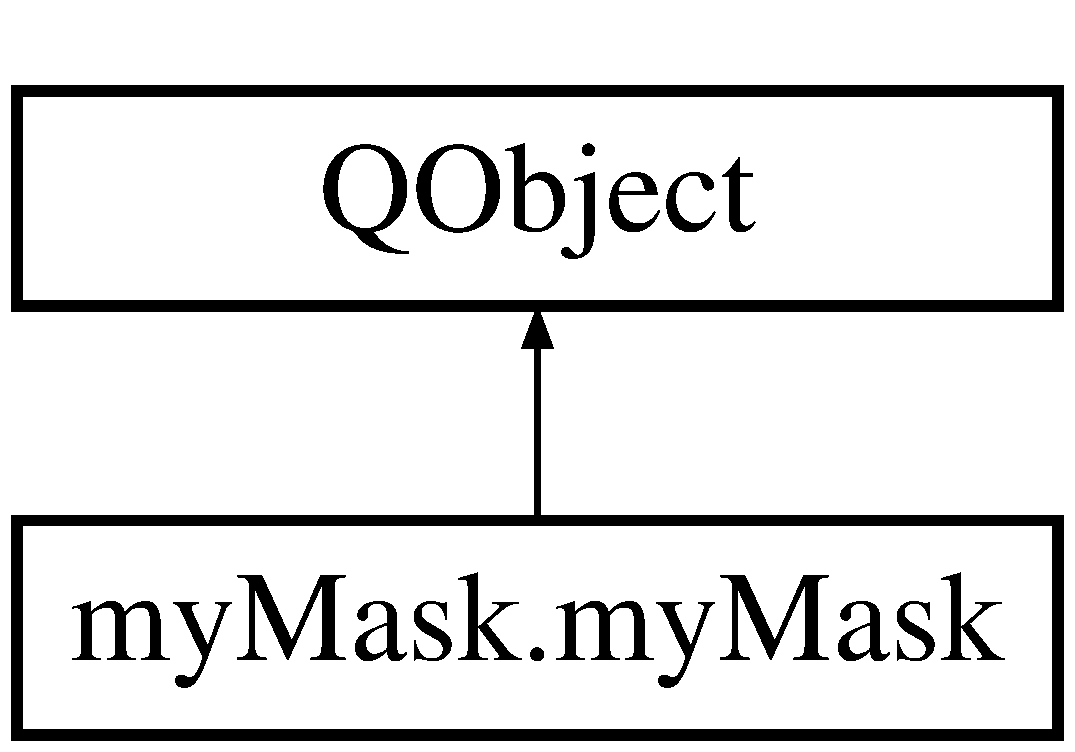
\includegraphics[height=2.000000cm]{classmy_mask_1_1my_mask}
\end{center}
\end{figure}
\subsection*{Public Member Functions}
\begin{DoxyCompactItemize}
\item 
def \hyperlink{classmy_mask_1_1my_mask_a551d04051af413888f60e9cf74a964fa}{create\-Mask}
\item 
def \hyperlink{classmy_mask_1_1my_mask_a0b6e02944d05baf74d75976672b75ba3}{set\-Mask}
\item 
def \hyperlink{classmy_mask_1_1my_mask_aaa9e1d93e4202095b0c5ffba2d98d53a}{reset\-Mask}
\item 
def \hyperlink{classmy_mask_1_1my_mask_a1b17be401eb92b7293e40de411f8b17f}{save\-To\-File}
\item 
def \hyperlink{classmy_mask_1_1my_mask_aface6241850e7cbc5bc4ae847e936eac}{read\-Tiff}
\end{DoxyCompactItemize}
\subsection*{Public Attributes}
\begin{DoxyCompactItemize}
\item 
\hyperlink{classmy_mask_1_1my_mask_abc71579b1017e1a3d98fdca371e771fd}{img}
\item 
\hyperlink{classmy_mask_1_1my_mask_aec05f7b9af1f9ba5b283f1034f229cdc}{nsamps}
\item 
\hyperlink{classmy_mask_1_1my_mask_a580ea0a4ec202bbc76ac0ad31b3d9f2b}{nlines}
\item 
\hyperlink{classmy_mask_1_1my_mask_a70decb30e8747e2688e1840f253f3950}{im\-File\-Name}
\end{DoxyCompactItemize}
\subsection*{Static Public Attributes}
\begin{DoxyCompactItemize}
\item 
int \hyperlink{classmy_mask_1_1my_mask_a6a94c13fe022b092f42d5be3f3b29fe6}{nsamps} = 0
\item 
int \hyperlink{classmy_mask_1_1my_mask_a91b9f3c41dd6f0c54860b24069f56ca4}{nlines} = 0
\end{DoxyCompactItemize}


\subsection{Member Function Documentation}
\hypertarget{classmy_mask_1_1my_mask_a551d04051af413888f60e9cf74a964fa}{\index{my\-Mask\-::my\-Mask@{my\-Mask\-::my\-Mask}!create\-Mask@{create\-Mask}}
\index{create\-Mask@{create\-Mask}!myMask::myMask@{my\-Mask\-::my\-Mask}}
\subsubsection[{create\-Mask}]{\setlength{\rightskip}{0pt plus 5cm}def my\-Mask.\-my\-Mask.\-create\-Mask (
\begin{DoxyParamCaption}
\item[{}]{self, }
\item[{}]{nsamps, }
\item[{}]{nlines}
\end{DoxyParamCaption}
)}}\label{classmy_mask_1_1my_mask_a551d04051af413888f60e9cf74a964fa}
\hypertarget{classmy_mask_1_1my_mask_aface6241850e7cbc5bc4ae847e936eac}{\index{my\-Mask\-::my\-Mask@{my\-Mask\-::my\-Mask}!read\-Tiff@{read\-Tiff}}
\index{read\-Tiff@{read\-Tiff}!myMask::myMask@{my\-Mask\-::my\-Mask}}
\subsubsection[{read\-Tiff}]{\setlength{\rightskip}{0pt plus 5cm}def my\-Mask.\-my\-Mask.\-read\-Tiff (
\begin{DoxyParamCaption}
\item[{}]{self, }
\item[{}]{infile}
\end{DoxyParamCaption}
)}}\label{classmy_mask_1_1my_mask_aface6241850e7cbc5bc4ae847e936eac}
\hypertarget{classmy_mask_1_1my_mask_aaa9e1d93e4202095b0c5ffba2d98d53a}{\index{my\-Mask\-::my\-Mask@{my\-Mask\-::my\-Mask}!reset\-Mask@{reset\-Mask}}
\index{reset\-Mask@{reset\-Mask}!myMask::myMask@{my\-Mask\-::my\-Mask}}
\subsubsection[{reset\-Mask}]{\setlength{\rightskip}{0pt plus 5cm}def my\-Mask.\-my\-Mask.\-reset\-Mask (
\begin{DoxyParamCaption}
\item[{}]{self}
\end{DoxyParamCaption}
)}}\label{classmy_mask_1_1my_mask_aaa9e1d93e4202095b0c5ffba2d98d53a}
\hypertarget{classmy_mask_1_1my_mask_a1b17be401eb92b7293e40de411f8b17f}{\index{my\-Mask\-::my\-Mask@{my\-Mask\-::my\-Mask}!save\-To\-File@{save\-To\-File}}
\index{save\-To\-File@{save\-To\-File}!myMask::myMask@{my\-Mask\-::my\-Mask}}
\subsubsection[{save\-To\-File}]{\setlength{\rightskip}{0pt plus 5cm}def my\-Mask.\-my\-Mask.\-save\-To\-File (
\begin{DoxyParamCaption}
\item[{}]{self, }
\item[{}]{fname}
\end{DoxyParamCaption}
)}}\label{classmy_mask_1_1my_mask_a1b17be401eb92b7293e40de411f8b17f}
\hypertarget{classmy_mask_1_1my_mask_a0b6e02944d05baf74d75976672b75ba3}{\index{my\-Mask\-::my\-Mask@{my\-Mask\-::my\-Mask}!set\-Mask@{set\-Mask}}
\index{set\-Mask@{set\-Mask}!myMask::myMask@{my\-Mask\-::my\-Mask}}
\subsubsection[{set\-Mask}]{\setlength{\rightskip}{0pt plus 5cm}def my\-Mask.\-my\-Mask.\-set\-Mask (
\begin{DoxyParamCaption}
\item[{}]{self, }
\item[{}]{rect, }
\item[{}]{mask\-Mode}
\end{DoxyParamCaption}
)}}\label{classmy_mask_1_1my_mask_a0b6e02944d05baf74d75976672b75ba3}


\subsection{Member Data Documentation}
\hypertarget{classmy_mask_1_1my_mask_a70decb30e8747e2688e1840f253f3950}{\index{my\-Mask\-::my\-Mask@{my\-Mask\-::my\-Mask}!im\-File\-Name@{im\-File\-Name}}
\index{im\-File\-Name@{im\-File\-Name}!myMask::myMask@{my\-Mask\-::my\-Mask}}
\subsubsection[{im\-File\-Name}]{\setlength{\rightskip}{0pt plus 5cm}my\-Mask.\-my\-Mask.\-im\-File\-Name}}\label{classmy_mask_1_1my_mask_a70decb30e8747e2688e1840f253f3950}
\hypertarget{classmy_mask_1_1my_mask_abc71579b1017e1a3d98fdca371e771fd}{\index{my\-Mask\-::my\-Mask@{my\-Mask\-::my\-Mask}!img@{img}}
\index{img@{img}!myMask::myMask@{my\-Mask\-::my\-Mask}}
\subsubsection[{img}]{\setlength{\rightskip}{0pt plus 5cm}my\-Mask.\-my\-Mask.\-img}}\label{classmy_mask_1_1my_mask_abc71579b1017e1a3d98fdca371e771fd}
\hypertarget{classmy_mask_1_1my_mask_a91b9f3c41dd6f0c54860b24069f56ca4}{\index{my\-Mask\-::my\-Mask@{my\-Mask\-::my\-Mask}!nlines@{nlines}}
\index{nlines@{nlines}!myMask::myMask@{my\-Mask\-::my\-Mask}}
\subsubsection[{nlines}]{\setlength{\rightskip}{0pt plus 5cm}int my\-Mask.\-my\-Mask.\-nlines = 0\hspace{0.3cm}{\ttfamily [static]}}}\label{classmy_mask_1_1my_mask_a91b9f3c41dd6f0c54860b24069f56ca4}
\hypertarget{classmy_mask_1_1my_mask_a580ea0a4ec202bbc76ac0ad31b3d9f2b}{\index{my\-Mask\-::my\-Mask@{my\-Mask\-::my\-Mask}!nlines@{nlines}}
\index{nlines@{nlines}!myMask::myMask@{my\-Mask\-::my\-Mask}}
\subsubsection[{nlines}]{\setlength{\rightskip}{0pt plus 5cm}my\-Mask.\-my\-Mask.\-nlines}}\label{classmy_mask_1_1my_mask_a580ea0a4ec202bbc76ac0ad31b3d9f2b}
\hypertarget{classmy_mask_1_1my_mask_a6a94c13fe022b092f42d5be3f3b29fe6}{\index{my\-Mask\-::my\-Mask@{my\-Mask\-::my\-Mask}!nsamps@{nsamps}}
\index{nsamps@{nsamps}!myMask::myMask@{my\-Mask\-::my\-Mask}}
\subsubsection[{nsamps}]{\setlength{\rightskip}{0pt plus 5cm}int my\-Mask.\-my\-Mask.\-nsamps = 0\hspace{0.3cm}{\ttfamily [static]}}}\label{classmy_mask_1_1my_mask_a6a94c13fe022b092f42d5be3f3b29fe6}
\hypertarget{classmy_mask_1_1my_mask_aec05f7b9af1f9ba5b283f1034f229cdc}{\index{my\-Mask\-::my\-Mask@{my\-Mask\-::my\-Mask}!nsamps@{nsamps}}
\index{nsamps@{nsamps}!myMask::myMask@{my\-Mask\-::my\-Mask}}
\subsubsection[{nsamps}]{\setlength{\rightskip}{0pt plus 5cm}my\-Mask.\-my\-Mask.\-nsamps}}\label{classmy_mask_1_1my_mask_aec05f7b9af1f9ba5b283f1034f229cdc}


The documentation for this class was generated from the following file\-:\begin{DoxyCompactItemize}
\item 
workdir/atrex/\-Software/\hyperlink{my_mask_8py}{my\-Mask.\-py}\end{DoxyCompactItemize}

\hypertarget{class_my_overlay_dlg_1_1_my_overlay_dlg}{\section{My\-Overlay\-Dlg.\-My\-Overlay\-Dlg Class Reference}
\label{class_my_overlay_dlg_1_1_my_overlay_dlg}\index{My\-Overlay\-Dlg.\-My\-Overlay\-Dlg@{My\-Overlay\-Dlg.\-My\-Overlay\-Dlg}}
}
Inheritance diagram for My\-Overlay\-Dlg.\-My\-Overlay\-Dlg\-:\begin{figure}[H]
\begin{center}
\leavevmode
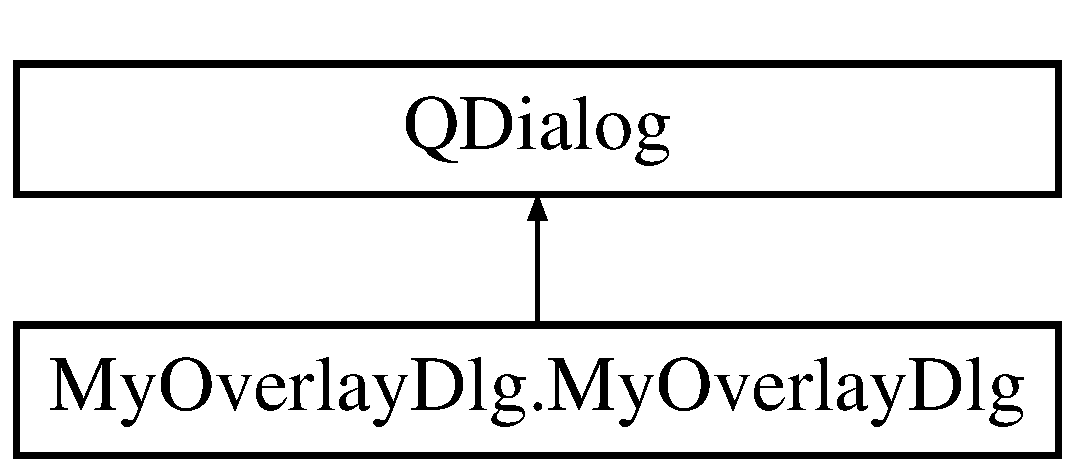
\includegraphics[height=2.000000cm]{class_my_overlay_dlg_1_1_my_overlay_dlg}
\end{center}
\end{figure}
\subsection*{Public Member Functions}
\begin{DoxyCompactItemize}
\item 
def \hyperlink{class_my_overlay_dlg_1_1_my_overlay_dlg_a836f26cd68556b2b577ba8ebbc36892a}{\-\_\-\-\_\-init\-\_\-\-\_\-}
\item 
def \hyperlink{class_my_overlay_dlg_1_1_my_overlay_dlg_a30489fcaa881f5dccddcc4782a1fcb2e}{set\-Params}
\item 
def \hyperlink{class_my_overlay_dlg_1_1_my_overlay_dlg_a911fbf22d0431f251fedbc1cc9ceee34}{accept}
\item 
def \hyperlink{class_my_overlay_dlg_1_1_my_overlay_dlg_a6b58d65c0fb4398f5187d9636723d4fd}{browse\-File}
\end{DoxyCompactItemize}
\subsection*{Public Attributes}
\begin{DoxyCompactItemize}
\item 
\hyperlink{class_my_overlay_dlg_1_1_my_overlay_dlg_a7d657b769e24e56ee48781d352de441e}{ui}
\item 
\hyperlink{class_my_overlay_dlg_1_1_my_overlay_dlg_acca8e0275695cf61524525634591381b}{infile}
\end{DoxyCompactItemize}
\subsection*{Static Public Attributes}
\begin{DoxyCompactItemize}
\item 
\hyperlink{class_my_overlay_dlg_1_1_my_overlay_dlg_a90f6e4408789fb09a8373122658e9dda}{second\-Flag} = False
\item 
string \hyperlink{class_my_overlay_dlg_1_1_my_overlay_dlg_a9a655828844f2260620132477ff6e2ac}{infile} = \char`\"{}\char`\"{}
\end{DoxyCompactItemize}


\subsection{Constructor \& Destructor Documentation}
\hypertarget{class_my_overlay_dlg_1_1_my_overlay_dlg_a836f26cd68556b2b577ba8ebbc36892a}{\index{My\-Overlay\-Dlg\-::\-My\-Overlay\-Dlg@{My\-Overlay\-Dlg\-::\-My\-Overlay\-Dlg}!\-\_\-\-\_\-init\-\_\-\-\_\-@{\-\_\-\-\_\-init\-\_\-\-\_\-}}
\index{\-\_\-\-\_\-init\-\_\-\-\_\-@{\-\_\-\-\_\-init\-\_\-\-\_\-}!MyOverlayDlg::MyOverlayDlg@{My\-Overlay\-Dlg\-::\-My\-Overlay\-Dlg}}
\subsubsection[{\-\_\-\-\_\-init\-\_\-\-\_\-}]{\setlength{\rightskip}{0pt plus 5cm}def My\-Overlay\-Dlg.\-My\-Overlay\-Dlg.\-\_\-\-\_\-init\-\_\-\-\_\- (
\begin{DoxyParamCaption}
\item[{}]{self}
\end{DoxyParamCaption}
)}}\label{class_my_overlay_dlg_1_1_my_overlay_dlg_a836f26cd68556b2b577ba8ebbc36892a}


\subsection{Member Function Documentation}
\hypertarget{class_my_overlay_dlg_1_1_my_overlay_dlg_a911fbf22d0431f251fedbc1cc9ceee34}{\index{My\-Overlay\-Dlg\-::\-My\-Overlay\-Dlg@{My\-Overlay\-Dlg\-::\-My\-Overlay\-Dlg}!accept@{accept}}
\index{accept@{accept}!MyOverlayDlg::MyOverlayDlg@{My\-Overlay\-Dlg\-::\-My\-Overlay\-Dlg}}
\subsubsection[{accept}]{\setlength{\rightskip}{0pt plus 5cm}def My\-Overlay\-Dlg.\-My\-Overlay\-Dlg.\-accept (
\begin{DoxyParamCaption}
\item[{}]{self}
\end{DoxyParamCaption}
)}}\label{class_my_overlay_dlg_1_1_my_overlay_dlg_a911fbf22d0431f251fedbc1cc9ceee34}
\hypertarget{class_my_overlay_dlg_1_1_my_overlay_dlg_a6b58d65c0fb4398f5187d9636723d4fd}{\index{My\-Overlay\-Dlg\-::\-My\-Overlay\-Dlg@{My\-Overlay\-Dlg\-::\-My\-Overlay\-Dlg}!browse\-File@{browse\-File}}
\index{browse\-File@{browse\-File}!MyOverlayDlg::MyOverlayDlg@{My\-Overlay\-Dlg\-::\-My\-Overlay\-Dlg}}
\subsubsection[{browse\-File}]{\setlength{\rightskip}{0pt plus 5cm}def My\-Overlay\-Dlg.\-My\-Overlay\-Dlg.\-browse\-File (
\begin{DoxyParamCaption}
\item[{}]{self}
\end{DoxyParamCaption}
)}}\label{class_my_overlay_dlg_1_1_my_overlay_dlg_a6b58d65c0fb4398f5187d9636723d4fd}
\hypertarget{class_my_overlay_dlg_1_1_my_overlay_dlg_a30489fcaa881f5dccddcc4782a1fcb2e}{\index{My\-Overlay\-Dlg\-::\-My\-Overlay\-Dlg@{My\-Overlay\-Dlg\-::\-My\-Overlay\-Dlg}!set\-Params@{set\-Params}}
\index{set\-Params@{set\-Params}!MyOverlayDlg::MyOverlayDlg@{My\-Overlay\-Dlg\-::\-My\-Overlay\-Dlg}}
\subsubsection[{set\-Params}]{\setlength{\rightskip}{0pt plus 5cm}def My\-Overlay\-Dlg.\-My\-Overlay\-Dlg.\-set\-Params (
\begin{DoxyParamCaption}
\item[{}]{self, }
\item[{}]{infl, }
\item[{}]{sflag}
\end{DoxyParamCaption}
)}}\label{class_my_overlay_dlg_1_1_my_overlay_dlg_a30489fcaa881f5dccddcc4782a1fcb2e}


\subsection{Member Data Documentation}
\hypertarget{class_my_overlay_dlg_1_1_my_overlay_dlg_a9a655828844f2260620132477ff6e2ac}{\index{My\-Overlay\-Dlg\-::\-My\-Overlay\-Dlg@{My\-Overlay\-Dlg\-::\-My\-Overlay\-Dlg}!infile@{infile}}
\index{infile@{infile}!MyOverlayDlg::MyOverlayDlg@{My\-Overlay\-Dlg\-::\-My\-Overlay\-Dlg}}
\subsubsection[{infile}]{\setlength{\rightskip}{0pt plus 5cm}string My\-Overlay\-Dlg.\-My\-Overlay\-Dlg.\-infile = \char`\"{}\char`\"{}\hspace{0.3cm}{\ttfamily [static]}}}\label{class_my_overlay_dlg_1_1_my_overlay_dlg_a9a655828844f2260620132477ff6e2ac}
\hypertarget{class_my_overlay_dlg_1_1_my_overlay_dlg_acca8e0275695cf61524525634591381b}{\index{My\-Overlay\-Dlg\-::\-My\-Overlay\-Dlg@{My\-Overlay\-Dlg\-::\-My\-Overlay\-Dlg}!infile@{infile}}
\index{infile@{infile}!MyOverlayDlg::MyOverlayDlg@{My\-Overlay\-Dlg\-::\-My\-Overlay\-Dlg}}
\subsubsection[{infile}]{\setlength{\rightskip}{0pt plus 5cm}My\-Overlay\-Dlg.\-My\-Overlay\-Dlg.\-infile}}\label{class_my_overlay_dlg_1_1_my_overlay_dlg_acca8e0275695cf61524525634591381b}
\hypertarget{class_my_overlay_dlg_1_1_my_overlay_dlg_a90f6e4408789fb09a8373122658e9dda}{\index{My\-Overlay\-Dlg\-::\-My\-Overlay\-Dlg@{My\-Overlay\-Dlg\-::\-My\-Overlay\-Dlg}!second\-Flag@{second\-Flag}}
\index{second\-Flag@{second\-Flag}!MyOverlayDlg::MyOverlayDlg@{My\-Overlay\-Dlg\-::\-My\-Overlay\-Dlg}}
\subsubsection[{second\-Flag}]{\setlength{\rightskip}{0pt plus 5cm}My\-Overlay\-Dlg.\-My\-Overlay\-Dlg.\-second\-Flag = False\hspace{0.3cm}{\ttfamily [static]}}}\label{class_my_overlay_dlg_1_1_my_overlay_dlg_a90f6e4408789fb09a8373122658e9dda}
\hypertarget{class_my_overlay_dlg_1_1_my_overlay_dlg_a7d657b769e24e56ee48781d352de441e}{\index{My\-Overlay\-Dlg\-::\-My\-Overlay\-Dlg@{My\-Overlay\-Dlg\-::\-My\-Overlay\-Dlg}!ui@{ui}}
\index{ui@{ui}!MyOverlayDlg::MyOverlayDlg@{My\-Overlay\-Dlg\-::\-My\-Overlay\-Dlg}}
\subsubsection[{ui}]{\setlength{\rightskip}{0pt plus 5cm}My\-Overlay\-Dlg.\-My\-Overlay\-Dlg.\-ui}}\label{class_my_overlay_dlg_1_1_my_overlay_dlg_a7d657b769e24e56ee48781d352de441e}


The documentation for this class was generated from the following file\-:\begin{DoxyCompactItemize}
\item 
workdir/atrex/\-Software/\hyperlink{_my_overlay_dlg_8py}{My\-Overlay\-Dlg.\-py}\end{DoxyCompactItemize}

\hypertarget{classmy_peak_table_1_1my_peak}{\section{my\-Peak\-Table.\-my\-Peak Class Reference}
\label{classmy_peak_table_1_1my_peak}\index{my\-Peak\-Table.\-my\-Peak@{my\-Peak\-Table.\-my\-Peak}}
}
\subsection*{Public Member Functions}
\begin{DoxyCompactItemize}
\item 
def \hyperlink{classmy_peak_table_1_1my_peak_a037a4088033f2adfaaa74c7352f70f48}{\-\_\-\-\_\-init\-\_\-\-\_\-}
\item 
def \hyperlink{classmy_peak_table_1_1my_peak_ad3e58261d15c3ac0e64876ce79e2fb65}{set\-Detxy}
\item 
def \hyperlink{classmy_peak_table_1_1my_peak_a69641e1873ad1aeb01e9addef6aee25b}{get\-Detxy}
\item 
def \hyperlink{classmy_peak_table_1_1my_peak_acd0cd543ea0c89c12ab6a336b1898f8c}{isselected}
\item 
def \hyperlink{classmy_peak_table_1_1my_peak_a95656972d93036d4f594a8dffa41ac1a}{distance}
\end{DoxyCompactItemize}
\subsection*{Public Attributes}
\begin{DoxyCompactItemize}
\item 
\hyperlink{classmy_peak_table_1_1my_peak_a7c51e9bdbae2d5de7166bd7c3e3b65c7}{Stat}
\item 
\hyperlink{classmy_peak_table_1_1my_peak_a4f83f9dd7d111bbcde0252dc8d383da6}{H\-K\-L}
\item 
\hyperlink{classmy_peak_table_1_1my_peak_a8b31f75e94aeffb31d8d0fc8f19857a5}{X\-Y\-Z}
\item 
\hyperlink{classmy_peak_table_1_1my_peak_a645f6926432f2d6f2a3c2a0ccdf2dfba}{selected}
\item 
\hyperlink{classmy_peak_table_1_1my_peak_ac1b6e5261fd5b16e906d1d372d63d2ac}{Det\-X\-Y}
\item 
\hyperlink{classmy_peak_table_1_1my_peak_ab8e16077fdc1617a011bfa4352d6a598}{Gonio}
\item 
\hyperlink{classmy_peak_table_1_1my_peak_a0538d9973495e8eb05641dfe9ecac8b7}{Gonio\-S\-S}
\item 
\hyperlink{classmy_peak_table_1_1my_peak_a9c1b6178ca664594ee881dde502d2f32}{nen}
\item 
\hyperlink{classmy_peak_table_1_1my_peak_a1e3264f8b2be66613640bb06fade9ee2}{energies}
\item 
\hyperlink{classmy_peak_table_1_1my_peak_a65c10ab02db534ce64958dcd3a5a33af}{Int\-A\-D}
\item 
\hyperlink{classmy_peak_table_1_1my_peak_a14e93826d7c0fa3bce77caa61002d545}{position}
\item 
\hyperlink{classmy_peak_table_1_1my_peak_adc16c2a4085ac1d6c9f9b8332e964be1}{Int\-S\-S\-D}
\item 
\hyperlink{classmy_peak_table_1_1my_peak_a1ad3ef21887f7a8d2c5f55df901476bc}{Adp}
\item 
\hyperlink{classmy_peak_table_1_1my_peak_ab95d78c678d003d9ff47a47fcccf9bb2}{click\-Selected}
\end{DoxyCompactItemize}


\subsection{Constructor \& Destructor Documentation}
\hypertarget{classmy_peak_table_1_1my_peak_a037a4088033f2adfaaa74c7352f70f48}{\index{my\-Peak\-Table\-::my\-Peak@{my\-Peak\-Table\-::my\-Peak}!\-\_\-\-\_\-init\-\_\-\-\_\-@{\-\_\-\-\_\-init\-\_\-\-\_\-}}
\index{\-\_\-\-\_\-init\-\_\-\-\_\-@{\-\_\-\-\_\-init\-\_\-\-\_\-}!myPeakTable::myPeak@{my\-Peak\-Table\-::my\-Peak}}
\subsubsection[{\-\_\-\-\_\-init\-\_\-\-\_\-}]{\setlength{\rightskip}{0pt plus 5cm}def my\-Peak\-Table.\-my\-Peak.\-\_\-\-\_\-init\-\_\-\-\_\- (
\begin{DoxyParamCaption}
\item[{}]{self}
\end{DoxyParamCaption}
)}}\label{classmy_peak_table_1_1my_peak_a037a4088033f2adfaaa74c7352f70f48}


\subsection{Member Function Documentation}
\hypertarget{classmy_peak_table_1_1my_peak_a95656972d93036d4f594a8dffa41ac1a}{\index{my\-Peak\-Table\-::my\-Peak@{my\-Peak\-Table\-::my\-Peak}!distance@{distance}}
\index{distance@{distance}!myPeakTable::myPeak@{my\-Peak\-Table\-::my\-Peak}}
\subsubsection[{distance}]{\setlength{\rightskip}{0pt plus 5cm}def my\-Peak\-Table.\-my\-Peak.\-distance (
\begin{DoxyParamCaption}
\item[{}]{self, }
\item[{}]{peak}
\end{DoxyParamCaption}
)}}\label{classmy_peak_table_1_1my_peak_a95656972d93036d4f594a8dffa41ac1a}
\hypertarget{classmy_peak_table_1_1my_peak_a69641e1873ad1aeb01e9addef6aee25b}{\index{my\-Peak\-Table\-::my\-Peak@{my\-Peak\-Table\-::my\-Peak}!get\-Detxy@{get\-Detxy}}
\index{get\-Detxy@{get\-Detxy}!myPeakTable::myPeak@{my\-Peak\-Table\-::my\-Peak}}
\subsubsection[{get\-Detxy}]{\setlength{\rightskip}{0pt plus 5cm}def my\-Peak\-Table.\-my\-Peak.\-get\-Detxy (
\begin{DoxyParamCaption}
\item[{}]{self}
\end{DoxyParamCaption}
)}}\label{classmy_peak_table_1_1my_peak_a69641e1873ad1aeb01e9addef6aee25b}
\hypertarget{classmy_peak_table_1_1my_peak_acd0cd543ea0c89c12ab6a336b1898f8c}{\index{my\-Peak\-Table\-::my\-Peak@{my\-Peak\-Table\-::my\-Peak}!isselected@{isselected}}
\index{isselected@{isselected}!myPeakTable::myPeak@{my\-Peak\-Table\-::my\-Peak}}
\subsubsection[{isselected}]{\setlength{\rightskip}{0pt plus 5cm}def my\-Peak\-Table.\-my\-Peak.\-isselected (
\begin{DoxyParamCaption}
\item[{}]{self}
\end{DoxyParamCaption}
)}}\label{classmy_peak_table_1_1my_peak_acd0cd543ea0c89c12ab6a336b1898f8c}
\hypertarget{classmy_peak_table_1_1my_peak_ad3e58261d15c3ac0e64876ce79e2fb65}{\index{my\-Peak\-Table\-::my\-Peak@{my\-Peak\-Table\-::my\-Peak}!set\-Detxy@{set\-Detxy}}
\index{set\-Detxy@{set\-Detxy}!myPeakTable::myPeak@{my\-Peak\-Table\-::my\-Peak}}
\subsubsection[{set\-Detxy}]{\setlength{\rightskip}{0pt plus 5cm}def my\-Peak\-Table.\-my\-Peak.\-set\-Detxy (
\begin{DoxyParamCaption}
\item[{}]{self, }
\item[{}]{X\-Y}
\end{DoxyParamCaption}
)}}\label{classmy_peak_table_1_1my_peak_ad3e58261d15c3ac0e64876ce79e2fb65}


\subsection{Member Data Documentation}
\hypertarget{classmy_peak_table_1_1my_peak_a1ad3ef21887f7a8d2c5f55df901476bc}{\index{my\-Peak\-Table\-::my\-Peak@{my\-Peak\-Table\-::my\-Peak}!Adp@{Adp}}
\index{Adp@{Adp}!myPeakTable::myPeak@{my\-Peak\-Table\-::my\-Peak}}
\subsubsection[{Adp}]{\setlength{\rightskip}{0pt plus 5cm}my\-Peak\-Table.\-my\-Peak.\-Adp}}\label{classmy_peak_table_1_1my_peak_a1ad3ef21887f7a8d2c5f55df901476bc}
\hypertarget{classmy_peak_table_1_1my_peak_ab95d78c678d003d9ff47a47fcccf9bb2}{\index{my\-Peak\-Table\-::my\-Peak@{my\-Peak\-Table\-::my\-Peak}!click\-Selected@{click\-Selected}}
\index{click\-Selected@{click\-Selected}!myPeakTable::myPeak@{my\-Peak\-Table\-::my\-Peak}}
\subsubsection[{click\-Selected}]{\setlength{\rightskip}{0pt plus 5cm}my\-Peak\-Table.\-my\-Peak.\-click\-Selected}}\label{classmy_peak_table_1_1my_peak_ab95d78c678d003d9ff47a47fcccf9bb2}
\hypertarget{classmy_peak_table_1_1my_peak_ac1b6e5261fd5b16e906d1d372d63d2ac}{\index{my\-Peak\-Table\-::my\-Peak@{my\-Peak\-Table\-::my\-Peak}!Det\-X\-Y@{Det\-X\-Y}}
\index{Det\-X\-Y@{Det\-X\-Y}!myPeakTable::myPeak@{my\-Peak\-Table\-::my\-Peak}}
\subsubsection[{Det\-X\-Y}]{\setlength{\rightskip}{0pt plus 5cm}my\-Peak\-Table.\-my\-Peak.\-Det\-X\-Y}}\label{classmy_peak_table_1_1my_peak_ac1b6e5261fd5b16e906d1d372d63d2ac}
\hypertarget{classmy_peak_table_1_1my_peak_a1e3264f8b2be66613640bb06fade9ee2}{\index{my\-Peak\-Table\-::my\-Peak@{my\-Peak\-Table\-::my\-Peak}!energies@{energies}}
\index{energies@{energies}!myPeakTable::myPeak@{my\-Peak\-Table\-::my\-Peak}}
\subsubsection[{energies}]{\setlength{\rightskip}{0pt plus 5cm}my\-Peak\-Table.\-my\-Peak.\-energies}}\label{classmy_peak_table_1_1my_peak_a1e3264f8b2be66613640bb06fade9ee2}
\hypertarget{classmy_peak_table_1_1my_peak_ab8e16077fdc1617a011bfa4352d6a598}{\index{my\-Peak\-Table\-::my\-Peak@{my\-Peak\-Table\-::my\-Peak}!Gonio@{Gonio}}
\index{Gonio@{Gonio}!myPeakTable::myPeak@{my\-Peak\-Table\-::my\-Peak}}
\subsubsection[{Gonio}]{\setlength{\rightskip}{0pt plus 5cm}my\-Peak\-Table.\-my\-Peak.\-Gonio}}\label{classmy_peak_table_1_1my_peak_ab8e16077fdc1617a011bfa4352d6a598}
\hypertarget{classmy_peak_table_1_1my_peak_a0538d9973495e8eb05641dfe9ecac8b7}{\index{my\-Peak\-Table\-::my\-Peak@{my\-Peak\-Table\-::my\-Peak}!Gonio\-S\-S@{Gonio\-S\-S}}
\index{Gonio\-S\-S@{Gonio\-S\-S}!myPeakTable::myPeak@{my\-Peak\-Table\-::my\-Peak}}
\subsubsection[{Gonio\-S\-S}]{\setlength{\rightskip}{0pt plus 5cm}my\-Peak\-Table.\-my\-Peak.\-Gonio\-S\-S}}\label{classmy_peak_table_1_1my_peak_a0538d9973495e8eb05641dfe9ecac8b7}
\hypertarget{classmy_peak_table_1_1my_peak_a4f83f9dd7d111bbcde0252dc8d383da6}{\index{my\-Peak\-Table\-::my\-Peak@{my\-Peak\-Table\-::my\-Peak}!H\-K\-L@{H\-K\-L}}
\index{H\-K\-L@{H\-K\-L}!myPeakTable::myPeak@{my\-Peak\-Table\-::my\-Peak}}
\subsubsection[{H\-K\-L}]{\setlength{\rightskip}{0pt plus 5cm}my\-Peak\-Table.\-my\-Peak.\-H\-K\-L}}\label{classmy_peak_table_1_1my_peak_a4f83f9dd7d111bbcde0252dc8d383da6}
\hypertarget{classmy_peak_table_1_1my_peak_a65c10ab02db534ce64958dcd3a5a33af}{\index{my\-Peak\-Table\-::my\-Peak@{my\-Peak\-Table\-::my\-Peak}!Int\-A\-D@{Int\-A\-D}}
\index{Int\-A\-D@{Int\-A\-D}!myPeakTable::myPeak@{my\-Peak\-Table\-::my\-Peak}}
\subsubsection[{Int\-A\-D}]{\setlength{\rightskip}{0pt plus 5cm}my\-Peak\-Table.\-my\-Peak.\-Int\-A\-D}}\label{classmy_peak_table_1_1my_peak_a65c10ab02db534ce64958dcd3a5a33af}
\hypertarget{classmy_peak_table_1_1my_peak_adc16c2a4085ac1d6c9f9b8332e964be1}{\index{my\-Peak\-Table\-::my\-Peak@{my\-Peak\-Table\-::my\-Peak}!Int\-S\-S\-D@{Int\-S\-S\-D}}
\index{Int\-S\-S\-D@{Int\-S\-S\-D}!myPeakTable::myPeak@{my\-Peak\-Table\-::my\-Peak}}
\subsubsection[{Int\-S\-S\-D}]{\setlength{\rightskip}{0pt plus 5cm}my\-Peak\-Table.\-my\-Peak.\-Int\-S\-S\-D}}\label{classmy_peak_table_1_1my_peak_adc16c2a4085ac1d6c9f9b8332e964be1}
\hypertarget{classmy_peak_table_1_1my_peak_a9c1b6178ca664594ee881dde502d2f32}{\index{my\-Peak\-Table\-::my\-Peak@{my\-Peak\-Table\-::my\-Peak}!nen@{nen}}
\index{nen@{nen}!myPeakTable::myPeak@{my\-Peak\-Table\-::my\-Peak}}
\subsubsection[{nen}]{\setlength{\rightskip}{0pt plus 5cm}my\-Peak\-Table.\-my\-Peak.\-nen}}\label{classmy_peak_table_1_1my_peak_a9c1b6178ca664594ee881dde502d2f32}
\hypertarget{classmy_peak_table_1_1my_peak_a14e93826d7c0fa3bce77caa61002d545}{\index{my\-Peak\-Table\-::my\-Peak@{my\-Peak\-Table\-::my\-Peak}!position@{position}}
\index{position@{position}!myPeakTable::myPeak@{my\-Peak\-Table\-::my\-Peak}}
\subsubsection[{position}]{\setlength{\rightskip}{0pt plus 5cm}my\-Peak\-Table.\-my\-Peak.\-position}}\label{classmy_peak_table_1_1my_peak_a14e93826d7c0fa3bce77caa61002d545}
\hypertarget{classmy_peak_table_1_1my_peak_a645f6926432f2d6f2a3c2a0ccdf2dfba}{\index{my\-Peak\-Table\-::my\-Peak@{my\-Peak\-Table\-::my\-Peak}!selected@{selected}}
\index{selected@{selected}!myPeakTable::myPeak@{my\-Peak\-Table\-::my\-Peak}}
\subsubsection[{selected}]{\setlength{\rightskip}{0pt plus 5cm}my\-Peak\-Table.\-my\-Peak.\-selected}}\label{classmy_peak_table_1_1my_peak_a645f6926432f2d6f2a3c2a0ccdf2dfba}
\hypertarget{classmy_peak_table_1_1my_peak_a7c51e9bdbae2d5de7166bd7c3e3b65c7}{\index{my\-Peak\-Table\-::my\-Peak@{my\-Peak\-Table\-::my\-Peak}!Stat@{Stat}}
\index{Stat@{Stat}!myPeakTable::myPeak@{my\-Peak\-Table\-::my\-Peak}}
\subsubsection[{Stat}]{\setlength{\rightskip}{0pt plus 5cm}my\-Peak\-Table.\-my\-Peak.\-Stat}}\label{classmy_peak_table_1_1my_peak_a7c51e9bdbae2d5de7166bd7c3e3b65c7}
\hypertarget{classmy_peak_table_1_1my_peak_a8b31f75e94aeffb31d8d0fc8f19857a5}{\index{my\-Peak\-Table\-::my\-Peak@{my\-Peak\-Table\-::my\-Peak}!X\-Y\-Z@{X\-Y\-Z}}
\index{X\-Y\-Z@{X\-Y\-Z}!myPeakTable::myPeak@{my\-Peak\-Table\-::my\-Peak}}
\subsubsection[{X\-Y\-Z}]{\setlength{\rightskip}{0pt plus 5cm}my\-Peak\-Table.\-my\-Peak.\-X\-Y\-Z}}\label{classmy_peak_table_1_1my_peak_a8b31f75e94aeffb31d8d0fc8f19857a5}


The documentation for this class was generated from the following file\-:\begin{DoxyCompactItemize}
\item 
workdir/atrex/\-Software/\hyperlink{my_peak_table_8py}{my\-Peak\-Table.\-py}\end{DoxyCompactItemize}

\hypertarget{classmy_peak_adjust_dlg_1_1my_peak_adjust_dlg}{\section{my\-Peak\-Adjust\-Dlg.\-my\-Peak\-Adjust\-Dlg Class Reference}
\label{classmy_peak_adjust_dlg_1_1my_peak_adjust_dlg}\index{my\-Peak\-Adjust\-Dlg.\-my\-Peak\-Adjust\-Dlg@{my\-Peak\-Adjust\-Dlg.\-my\-Peak\-Adjust\-Dlg}}
}
Inheritance diagram for my\-Peak\-Adjust\-Dlg.\-my\-Peak\-Adjust\-Dlg\-:\begin{figure}[H]
\begin{center}
\leavevmode
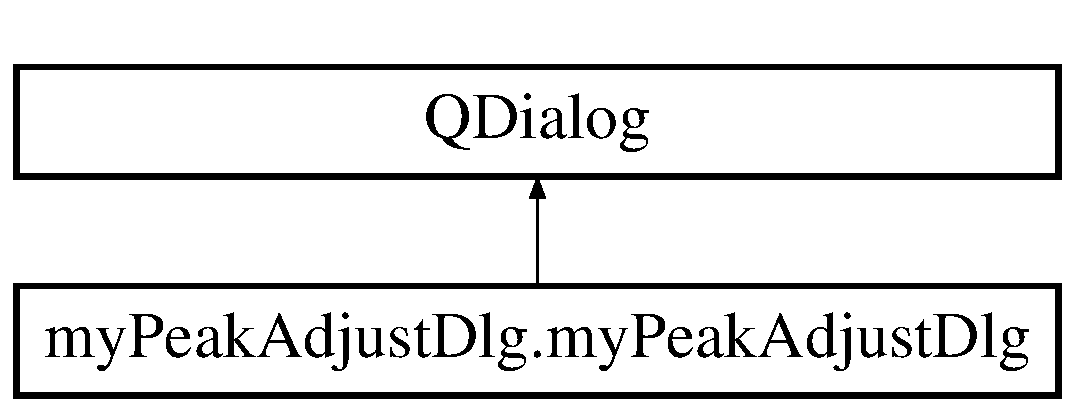
\includegraphics[height=2.000000cm]{classmy_peak_adjust_dlg_1_1my_peak_adjust_dlg}
\end{center}
\end{figure}
\subsection*{Public Member Functions}
\begin{DoxyCompactItemize}
\item 
def \hyperlink{classmy_peak_adjust_dlg_1_1my_peak_adjust_dlg_abaacb5b4b52585a3c95c3709c7ddc87a}{\-\_\-\-\_\-init\-\_\-\-\_\-}
\item 
def \hyperlink{classmy_peak_adjust_dlg_1_1my_peak_adjust_dlg_a8a3b1f75dfe5592add8cf68686659a41}{set\-Peak\-Display}
\item 
def \hyperlink{classmy_peak_adjust_dlg_1_1my_peak_adjust_dlg_a5ff4c61e897515906ea1cf647a8ebb4e}{changed\-Type}
\item 
def \hyperlink{classmy_peak_adjust_dlg_1_1my_peak_adjust_dlg_ad3012bad6f6dbe3c06af6758dab86acb}{update\-L\-E\-Fields}
\item 
def \hyperlink{classmy_peak_adjust_dlg_1_1my_peak_adjust_dlg_afde46489a42cbb16452829ef81097005}{update}
\end{DoxyCompactItemize}
\subsection*{Public Attributes}
\begin{DoxyCompactItemize}
\item 
\hyperlink{classmy_peak_adjust_dlg_1_1my_peak_adjust_dlg_a1fc76ecbe349bc391603074a7b2ca8c9}{ui}
\item 
\hyperlink{classmy_peak_adjust_dlg_1_1my_peak_adjust_dlg_af1e548deba0b44e985b04f37f53f4976}{zm\-Peak\-Fit}
\item 
\hyperlink{classmy_peak_adjust_dlg_1_1my_peak_adjust_dlg_a4c928c7791bd418243581ae926f275b6}{zm\-Peak\-Resids}
\end{DoxyCompactItemize}
\subsection*{Static Public Attributes}
\begin{DoxyCompactItemize}
\item 
\hyperlink{classmy_peak_adjust_dlg_1_1my_peak_adjust_dlg_a9c226539269d6b35d50880d49e49dff7}{zm\-Peak\-Raw} = None
\item 
list \hyperlink{classmy_peak_adjust_dlg_1_1my_peak_adjust_dlg_a77033ff8fcc0c925aafb76333050f5c9}{raw\-Mn\-Mx} = \mbox{[}0.,0.\mbox{]}
\item 
list \hyperlink{classmy_peak_adjust_dlg_1_1my_peak_adjust_dlg_a50b584afc0dbc9e5c7dc296325469935}{fit\-Mn\-Mx} = \mbox{[}0.,0.\mbox{]}
\item 
list \hyperlink{classmy_peak_adjust_dlg_1_1my_peak_adjust_dlg_a50a4c1e4d7862bb9d67565279fc9ed6e}{resids\-Mn\-Mx} = \mbox{[}0.,0.\mbox{]}
\end{DoxyCompactItemize}


\subsection{Constructor \& Destructor Documentation}
\hypertarget{classmy_peak_adjust_dlg_1_1my_peak_adjust_dlg_abaacb5b4b52585a3c95c3709c7ddc87a}{\index{my\-Peak\-Adjust\-Dlg\-::my\-Peak\-Adjust\-Dlg@{my\-Peak\-Adjust\-Dlg\-::my\-Peak\-Adjust\-Dlg}!\-\_\-\-\_\-init\-\_\-\-\_\-@{\-\_\-\-\_\-init\-\_\-\-\_\-}}
\index{\-\_\-\-\_\-init\-\_\-\-\_\-@{\-\_\-\-\_\-init\-\_\-\-\_\-}!myPeakAdjustDlg::myPeakAdjustDlg@{my\-Peak\-Adjust\-Dlg\-::my\-Peak\-Adjust\-Dlg}}
\subsubsection[{\-\_\-\-\_\-init\-\_\-\-\_\-}]{\setlength{\rightskip}{0pt plus 5cm}def my\-Peak\-Adjust\-Dlg.\-my\-Peak\-Adjust\-Dlg.\-\_\-\-\_\-init\-\_\-\-\_\- (
\begin{DoxyParamCaption}
\item[{}]{self}
\end{DoxyParamCaption}
)}}\label{classmy_peak_adjust_dlg_1_1my_peak_adjust_dlg_abaacb5b4b52585a3c95c3709c7ddc87a}


\subsection{Member Function Documentation}
\hypertarget{classmy_peak_adjust_dlg_1_1my_peak_adjust_dlg_a5ff4c61e897515906ea1cf647a8ebb4e}{\index{my\-Peak\-Adjust\-Dlg\-::my\-Peak\-Adjust\-Dlg@{my\-Peak\-Adjust\-Dlg\-::my\-Peak\-Adjust\-Dlg}!changed\-Type@{changed\-Type}}
\index{changed\-Type@{changed\-Type}!myPeakAdjustDlg::myPeakAdjustDlg@{my\-Peak\-Adjust\-Dlg\-::my\-Peak\-Adjust\-Dlg}}
\subsubsection[{changed\-Type}]{\setlength{\rightskip}{0pt plus 5cm}def my\-Peak\-Adjust\-Dlg.\-my\-Peak\-Adjust\-Dlg.\-changed\-Type (
\begin{DoxyParamCaption}
\item[{}]{self, }
\item[{}]{bval}
\end{DoxyParamCaption}
)}}\label{classmy_peak_adjust_dlg_1_1my_peak_adjust_dlg_a5ff4c61e897515906ea1cf647a8ebb4e}
\hypertarget{classmy_peak_adjust_dlg_1_1my_peak_adjust_dlg_a8a3b1f75dfe5592add8cf68686659a41}{\index{my\-Peak\-Adjust\-Dlg\-::my\-Peak\-Adjust\-Dlg@{my\-Peak\-Adjust\-Dlg\-::my\-Peak\-Adjust\-Dlg}!set\-Peak\-Display@{set\-Peak\-Display}}
\index{set\-Peak\-Display@{set\-Peak\-Display}!myPeakAdjustDlg::myPeakAdjustDlg@{my\-Peak\-Adjust\-Dlg\-::my\-Peak\-Adjust\-Dlg}}
\subsubsection[{set\-Peak\-Display}]{\setlength{\rightskip}{0pt plus 5cm}def my\-Peak\-Adjust\-Dlg.\-my\-Peak\-Adjust\-Dlg.\-set\-Peak\-Display (
\begin{DoxyParamCaption}
\item[{}]{self, }
\item[{}]{type, }
\item[{}]{disp\-Widget}
\end{DoxyParamCaption}
)}}\label{classmy_peak_adjust_dlg_1_1my_peak_adjust_dlg_a8a3b1f75dfe5592add8cf68686659a41}
\hypertarget{classmy_peak_adjust_dlg_1_1my_peak_adjust_dlg_afde46489a42cbb16452829ef81097005}{\index{my\-Peak\-Adjust\-Dlg\-::my\-Peak\-Adjust\-Dlg@{my\-Peak\-Adjust\-Dlg\-::my\-Peak\-Adjust\-Dlg}!update@{update}}
\index{update@{update}!myPeakAdjustDlg::myPeakAdjustDlg@{my\-Peak\-Adjust\-Dlg\-::my\-Peak\-Adjust\-Dlg}}
\subsubsection[{update}]{\setlength{\rightskip}{0pt plus 5cm}def my\-Peak\-Adjust\-Dlg.\-my\-Peak\-Adjust\-Dlg.\-update (
\begin{DoxyParamCaption}
\item[{}]{self}
\end{DoxyParamCaption}
)}}\label{classmy_peak_adjust_dlg_1_1my_peak_adjust_dlg_afde46489a42cbb16452829ef81097005}
\hypertarget{classmy_peak_adjust_dlg_1_1my_peak_adjust_dlg_ad3012bad6f6dbe3c06af6758dab86acb}{\index{my\-Peak\-Adjust\-Dlg\-::my\-Peak\-Adjust\-Dlg@{my\-Peak\-Adjust\-Dlg\-::my\-Peak\-Adjust\-Dlg}!update\-L\-E\-Fields@{update\-L\-E\-Fields}}
\index{update\-L\-E\-Fields@{update\-L\-E\-Fields}!myPeakAdjustDlg::myPeakAdjustDlg@{my\-Peak\-Adjust\-Dlg\-::my\-Peak\-Adjust\-Dlg}}
\subsubsection[{update\-L\-E\-Fields}]{\setlength{\rightskip}{0pt plus 5cm}def my\-Peak\-Adjust\-Dlg.\-my\-Peak\-Adjust\-Dlg.\-update\-L\-E\-Fields (
\begin{DoxyParamCaption}
\item[{}]{self}
\end{DoxyParamCaption}
)}}\label{classmy_peak_adjust_dlg_1_1my_peak_adjust_dlg_ad3012bad6f6dbe3c06af6758dab86acb}


\subsection{Member Data Documentation}
\hypertarget{classmy_peak_adjust_dlg_1_1my_peak_adjust_dlg_a50b584afc0dbc9e5c7dc296325469935}{\index{my\-Peak\-Adjust\-Dlg\-::my\-Peak\-Adjust\-Dlg@{my\-Peak\-Adjust\-Dlg\-::my\-Peak\-Adjust\-Dlg}!fit\-Mn\-Mx@{fit\-Mn\-Mx}}
\index{fit\-Mn\-Mx@{fit\-Mn\-Mx}!myPeakAdjustDlg::myPeakAdjustDlg@{my\-Peak\-Adjust\-Dlg\-::my\-Peak\-Adjust\-Dlg}}
\subsubsection[{fit\-Mn\-Mx}]{\setlength{\rightskip}{0pt plus 5cm}list my\-Peak\-Adjust\-Dlg.\-my\-Peak\-Adjust\-Dlg.\-fit\-Mn\-Mx = \mbox{[}0.,0.\mbox{]}\hspace{0.3cm}{\ttfamily [static]}}}\label{classmy_peak_adjust_dlg_1_1my_peak_adjust_dlg_a50b584afc0dbc9e5c7dc296325469935}
\hypertarget{classmy_peak_adjust_dlg_1_1my_peak_adjust_dlg_a77033ff8fcc0c925aafb76333050f5c9}{\index{my\-Peak\-Adjust\-Dlg\-::my\-Peak\-Adjust\-Dlg@{my\-Peak\-Adjust\-Dlg\-::my\-Peak\-Adjust\-Dlg}!raw\-Mn\-Mx@{raw\-Mn\-Mx}}
\index{raw\-Mn\-Mx@{raw\-Mn\-Mx}!myPeakAdjustDlg::myPeakAdjustDlg@{my\-Peak\-Adjust\-Dlg\-::my\-Peak\-Adjust\-Dlg}}
\subsubsection[{raw\-Mn\-Mx}]{\setlength{\rightskip}{0pt plus 5cm}list my\-Peak\-Adjust\-Dlg.\-my\-Peak\-Adjust\-Dlg.\-raw\-Mn\-Mx = \mbox{[}0.,0.\mbox{]}\hspace{0.3cm}{\ttfamily [static]}}}\label{classmy_peak_adjust_dlg_1_1my_peak_adjust_dlg_a77033ff8fcc0c925aafb76333050f5c9}
\hypertarget{classmy_peak_adjust_dlg_1_1my_peak_adjust_dlg_a50a4c1e4d7862bb9d67565279fc9ed6e}{\index{my\-Peak\-Adjust\-Dlg\-::my\-Peak\-Adjust\-Dlg@{my\-Peak\-Adjust\-Dlg\-::my\-Peak\-Adjust\-Dlg}!resids\-Mn\-Mx@{resids\-Mn\-Mx}}
\index{resids\-Mn\-Mx@{resids\-Mn\-Mx}!myPeakAdjustDlg::myPeakAdjustDlg@{my\-Peak\-Adjust\-Dlg\-::my\-Peak\-Adjust\-Dlg}}
\subsubsection[{resids\-Mn\-Mx}]{\setlength{\rightskip}{0pt plus 5cm}list my\-Peak\-Adjust\-Dlg.\-my\-Peak\-Adjust\-Dlg.\-resids\-Mn\-Mx = \mbox{[}0.,0.\mbox{]}\hspace{0.3cm}{\ttfamily [static]}}}\label{classmy_peak_adjust_dlg_1_1my_peak_adjust_dlg_a50a4c1e4d7862bb9d67565279fc9ed6e}
\hypertarget{classmy_peak_adjust_dlg_1_1my_peak_adjust_dlg_a1fc76ecbe349bc391603074a7b2ca8c9}{\index{my\-Peak\-Adjust\-Dlg\-::my\-Peak\-Adjust\-Dlg@{my\-Peak\-Adjust\-Dlg\-::my\-Peak\-Adjust\-Dlg}!ui@{ui}}
\index{ui@{ui}!myPeakAdjustDlg::myPeakAdjustDlg@{my\-Peak\-Adjust\-Dlg\-::my\-Peak\-Adjust\-Dlg}}
\subsubsection[{ui}]{\setlength{\rightskip}{0pt plus 5cm}my\-Peak\-Adjust\-Dlg.\-my\-Peak\-Adjust\-Dlg.\-ui}}\label{classmy_peak_adjust_dlg_1_1my_peak_adjust_dlg_a1fc76ecbe349bc391603074a7b2ca8c9}
\hypertarget{classmy_peak_adjust_dlg_1_1my_peak_adjust_dlg_af1e548deba0b44e985b04f37f53f4976}{\index{my\-Peak\-Adjust\-Dlg\-::my\-Peak\-Adjust\-Dlg@{my\-Peak\-Adjust\-Dlg\-::my\-Peak\-Adjust\-Dlg}!zm\-Peak\-Fit@{zm\-Peak\-Fit}}
\index{zm\-Peak\-Fit@{zm\-Peak\-Fit}!myPeakAdjustDlg::myPeakAdjustDlg@{my\-Peak\-Adjust\-Dlg\-::my\-Peak\-Adjust\-Dlg}}
\subsubsection[{zm\-Peak\-Fit}]{\setlength{\rightskip}{0pt plus 5cm}my\-Peak\-Adjust\-Dlg.\-my\-Peak\-Adjust\-Dlg.\-zm\-Peak\-Fit}}\label{classmy_peak_adjust_dlg_1_1my_peak_adjust_dlg_af1e548deba0b44e985b04f37f53f4976}
\hypertarget{classmy_peak_adjust_dlg_1_1my_peak_adjust_dlg_a9c226539269d6b35d50880d49e49dff7}{\index{my\-Peak\-Adjust\-Dlg\-::my\-Peak\-Adjust\-Dlg@{my\-Peak\-Adjust\-Dlg\-::my\-Peak\-Adjust\-Dlg}!zm\-Peak\-Raw@{zm\-Peak\-Raw}}
\index{zm\-Peak\-Raw@{zm\-Peak\-Raw}!myPeakAdjustDlg::myPeakAdjustDlg@{my\-Peak\-Adjust\-Dlg\-::my\-Peak\-Adjust\-Dlg}}
\subsubsection[{zm\-Peak\-Raw}]{\setlength{\rightskip}{0pt plus 5cm}my\-Peak\-Adjust\-Dlg.\-my\-Peak\-Adjust\-Dlg.\-zm\-Peak\-Raw = None\hspace{0.3cm}{\ttfamily [static]}}}\label{classmy_peak_adjust_dlg_1_1my_peak_adjust_dlg_a9c226539269d6b35d50880d49e49dff7}
\hypertarget{classmy_peak_adjust_dlg_1_1my_peak_adjust_dlg_a4c928c7791bd418243581ae926f275b6}{\index{my\-Peak\-Adjust\-Dlg\-::my\-Peak\-Adjust\-Dlg@{my\-Peak\-Adjust\-Dlg\-::my\-Peak\-Adjust\-Dlg}!zm\-Peak\-Resids@{zm\-Peak\-Resids}}
\index{zm\-Peak\-Resids@{zm\-Peak\-Resids}!myPeakAdjustDlg::myPeakAdjustDlg@{my\-Peak\-Adjust\-Dlg\-::my\-Peak\-Adjust\-Dlg}}
\subsubsection[{zm\-Peak\-Resids}]{\setlength{\rightskip}{0pt plus 5cm}my\-Peak\-Adjust\-Dlg.\-my\-Peak\-Adjust\-Dlg.\-zm\-Peak\-Resids}}\label{classmy_peak_adjust_dlg_1_1my_peak_adjust_dlg_a4c928c7791bd418243581ae926f275b6}


The documentation for this class was generated from the following file\-:\begin{DoxyCompactItemize}
\item 
workdir/atrex/\-Software/\hyperlink{my_peak_adjust_dlg_8py}{my\-Peak\-Adjust\-Dlg.\-py}\end{DoxyCompactItemize}

\hypertarget{classmy_peaks_1_1my_peaks}{\section{my\-Peaks.\-my\-Peaks Class Reference}
\label{classmy_peaks_1_1my_peaks}\index{my\-Peaks.\-my\-Peaks@{my\-Peaks.\-my\-Peaks}}
}
Inheritance diagram for my\-Peaks.\-my\-Peaks\-:\begin{figure}[H]
\begin{center}
\leavevmode
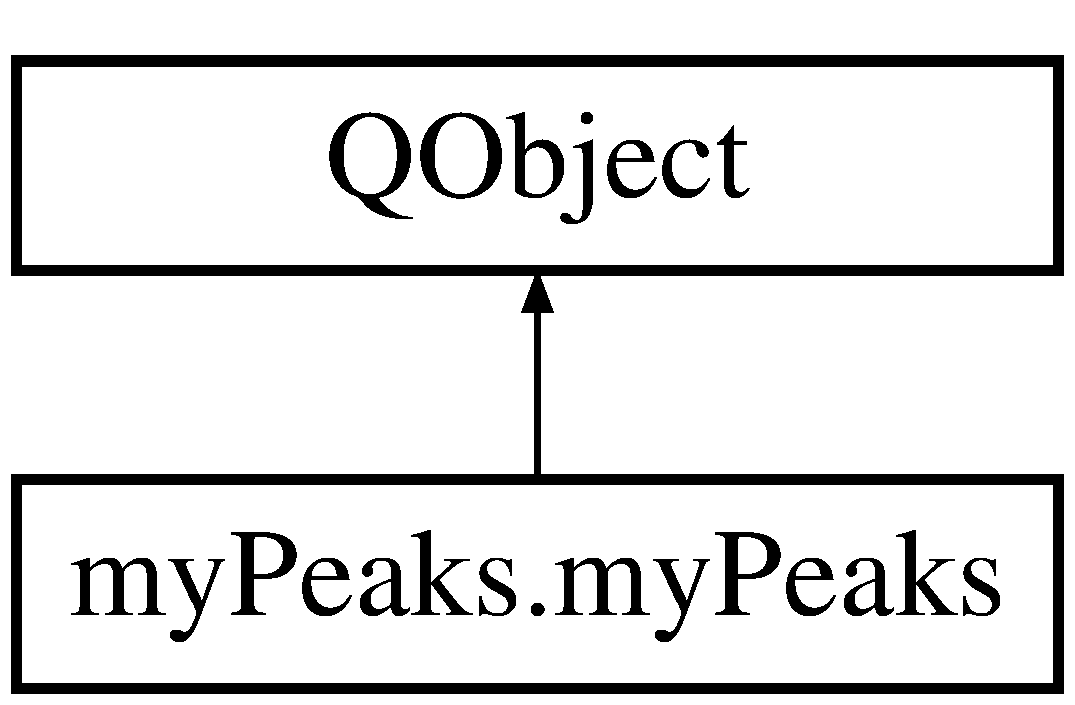
\includegraphics[height=2.000000cm]{classmy_peaks_1_1my_peaks}
\end{center}
\end{figure}
\subsection*{Public Member Functions}
\begin{DoxyCompactItemize}
\item 
def \hyperlink{classmy_peaks_1_1my_peaks_a96aa94100a2cae09e55aec9b21b5c934}{\-\_\-\-\_\-init\-\_\-\-\_\-}
\item 
def \hyperlink{classmy_peaks_1_1my_peaks_a85b8109b49ce283142c01c4f386657f5}{add\-Peak}
\item 
def \hyperlink{classmy_peaks_1_1my_peaks_a7f167f9ae163b0025f45f3552d238b4b}{set\-Active\-List}
\item 
def \hyperlink{classmy_peaks_1_1my_peaks_a8a2447225e6a87f1b0273697e633ba93}{set\-Selected}
\item 
def \hyperlink{classmy_peaks_1_1my_peaks_ab4288640f1dd2ea00b5aaa48d11014c4}{select\-All}
\item 
def \hyperlink{classmy_peaks_1_1my_peaks_aecd844074c5479e3379981ad71b85981}{clear\-All}
\item 
def \hyperlink{classmy_peaks_1_1my_peaks_a0da9e1901691583a56fb3784eedc91f7}{delete\-Selected}
\item 
def \hyperlink{classmy_peaks_1_1my_peaks_a90a5f3241c94520978668e1a3f62774e}{move\-Selected}
\end{DoxyCompactItemize}
\subsection*{Public Attributes}
\begin{DoxyCompactItemize}
\item 
\hyperlink{classmy_peaks_1_1my_peaks_ab764afe03c88786678b9b63fa09337ef}{active\-List}
\end{DoxyCompactItemize}
\subsection*{Static Public Attributes}
\begin{DoxyCompactItemize}
\item 
list \hyperlink{classmy_peaks_1_1my_peaks_a188582bdcbbda828a9d44fd7336570d8}{peaks\-\_\-0} = \mbox{[}$\,$\mbox{]}
\item 
list \hyperlink{classmy_peaks_1_1my_peaks_acba3b1f63dcd097b793f8cbcb0e0befc}{peaks\-\_\-1} = \mbox{[}$\,$\mbox{]}
\item 
list \hyperlink{classmy_peaks_1_1my_peaks_a769d8400c803069ed2de73079e5e8b08}{peak\-Lists} = \mbox{[}\hyperlink{classmy_peaks_1_1my_peaks_a188582bdcbbda828a9d44fd7336570d8}{peaks\-\_\-0},\hyperlink{classmy_peaks_1_1my_peaks_acba3b1f63dcd097b793f8cbcb0e0befc}{peaks\-\_\-1}\mbox{]}
\item 
int \hyperlink{classmy_peaks_1_1my_peaks_ae28250cdc31d2022b52ebd0b35b61ad9}{active\-List} = 0
\end{DoxyCompactItemize}


\subsection{Constructor \& Destructor Documentation}
\hypertarget{classmy_peaks_1_1my_peaks_a96aa94100a2cae09e55aec9b21b5c934}{\index{my\-Peaks\-::my\-Peaks@{my\-Peaks\-::my\-Peaks}!\-\_\-\-\_\-init\-\_\-\-\_\-@{\-\_\-\-\_\-init\-\_\-\-\_\-}}
\index{\-\_\-\-\_\-init\-\_\-\-\_\-@{\-\_\-\-\_\-init\-\_\-\-\_\-}!myPeaks::myPeaks@{my\-Peaks\-::my\-Peaks}}
\subsubsection[{\-\_\-\-\_\-init\-\_\-\-\_\-}]{\setlength{\rightskip}{0pt plus 5cm}def my\-Peaks.\-my\-Peaks.\-\_\-\-\_\-init\-\_\-\-\_\- (
\begin{DoxyParamCaption}
\item[{}]{self}
\end{DoxyParamCaption}
)}}\label{classmy_peaks_1_1my_peaks_a96aa94100a2cae09e55aec9b21b5c934}


\subsection{Member Function Documentation}
\hypertarget{classmy_peaks_1_1my_peaks_a85b8109b49ce283142c01c4f386657f5}{\index{my\-Peaks\-::my\-Peaks@{my\-Peaks\-::my\-Peaks}!add\-Peak@{add\-Peak}}
\index{add\-Peak@{add\-Peak}!myPeaks::myPeaks@{my\-Peaks\-::my\-Peaks}}
\subsubsection[{add\-Peak}]{\setlength{\rightskip}{0pt plus 5cm}def my\-Peaks.\-my\-Peaks.\-add\-Peak (
\begin{DoxyParamCaption}
\item[{}]{self, }
\item[{}]{x, }
\item[{}]{y}
\end{DoxyParamCaption}
)}}\label{classmy_peaks_1_1my_peaks_a85b8109b49ce283142c01c4f386657f5}
\hypertarget{classmy_peaks_1_1my_peaks_aecd844074c5479e3379981ad71b85981}{\index{my\-Peaks\-::my\-Peaks@{my\-Peaks\-::my\-Peaks}!clear\-All@{clear\-All}}
\index{clear\-All@{clear\-All}!myPeaks::myPeaks@{my\-Peaks\-::my\-Peaks}}
\subsubsection[{clear\-All}]{\setlength{\rightskip}{0pt plus 5cm}def my\-Peaks.\-my\-Peaks.\-clear\-All (
\begin{DoxyParamCaption}
\item[{}]{self}
\end{DoxyParamCaption}
)}}\label{classmy_peaks_1_1my_peaks_aecd844074c5479e3379981ad71b85981}
\hypertarget{classmy_peaks_1_1my_peaks_a0da9e1901691583a56fb3784eedc91f7}{\index{my\-Peaks\-::my\-Peaks@{my\-Peaks\-::my\-Peaks}!delete\-Selected@{delete\-Selected}}
\index{delete\-Selected@{delete\-Selected}!myPeaks::myPeaks@{my\-Peaks\-::my\-Peaks}}
\subsubsection[{delete\-Selected}]{\setlength{\rightskip}{0pt plus 5cm}def my\-Peaks.\-my\-Peaks.\-delete\-Selected (
\begin{DoxyParamCaption}
\item[{}]{self}
\end{DoxyParamCaption}
)}}\label{classmy_peaks_1_1my_peaks_a0da9e1901691583a56fb3784eedc91f7}
\hypertarget{classmy_peaks_1_1my_peaks_a90a5f3241c94520978668e1a3f62774e}{\index{my\-Peaks\-::my\-Peaks@{my\-Peaks\-::my\-Peaks}!move\-Selected@{move\-Selected}}
\index{move\-Selected@{move\-Selected}!myPeaks::myPeaks@{my\-Peaks\-::my\-Peaks}}
\subsubsection[{move\-Selected}]{\setlength{\rightskip}{0pt plus 5cm}def my\-Peaks.\-my\-Peaks.\-move\-Selected (
\begin{DoxyParamCaption}
\item[{}]{self}
\end{DoxyParamCaption}
)}}\label{classmy_peaks_1_1my_peaks_a90a5f3241c94520978668e1a3f62774e}
\hypertarget{classmy_peaks_1_1my_peaks_ab4288640f1dd2ea00b5aaa48d11014c4}{\index{my\-Peaks\-::my\-Peaks@{my\-Peaks\-::my\-Peaks}!select\-All@{select\-All}}
\index{select\-All@{select\-All}!myPeaks::myPeaks@{my\-Peaks\-::my\-Peaks}}
\subsubsection[{select\-All}]{\setlength{\rightskip}{0pt plus 5cm}def my\-Peaks.\-my\-Peaks.\-select\-All (
\begin{DoxyParamCaption}
\item[{}]{self}
\end{DoxyParamCaption}
)}}\label{classmy_peaks_1_1my_peaks_ab4288640f1dd2ea00b5aaa48d11014c4}
\hypertarget{classmy_peaks_1_1my_peaks_a7f167f9ae163b0025f45f3552d238b4b}{\index{my\-Peaks\-::my\-Peaks@{my\-Peaks\-::my\-Peaks}!set\-Active\-List@{set\-Active\-List}}
\index{set\-Active\-List@{set\-Active\-List}!myPeaks::myPeaks@{my\-Peaks\-::my\-Peaks}}
\subsubsection[{set\-Active\-List}]{\setlength{\rightskip}{0pt plus 5cm}def my\-Peaks.\-my\-Peaks.\-set\-Active\-List (
\begin{DoxyParamCaption}
\item[{}]{self, }
\item[{}]{ind}
\end{DoxyParamCaption}
)}}\label{classmy_peaks_1_1my_peaks_a7f167f9ae163b0025f45f3552d238b4b}
\hypertarget{classmy_peaks_1_1my_peaks_a8a2447225e6a87f1b0273697e633ba93}{\index{my\-Peaks\-::my\-Peaks@{my\-Peaks\-::my\-Peaks}!set\-Selected@{set\-Selected}}
\index{set\-Selected@{set\-Selected}!myPeaks::myPeaks@{my\-Peaks\-::my\-Peaks}}
\subsubsection[{set\-Selected}]{\setlength{\rightskip}{0pt plus 5cm}def my\-Peaks.\-my\-Peaks.\-set\-Selected (
\begin{DoxyParamCaption}
\item[{}]{self, }
\item[{}]{rect\-Coords}
\end{DoxyParamCaption}
)}}\label{classmy_peaks_1_1my_peaks_a8a2447225e6a87f1b0273697e633ba93}


\subsection{Member Data Documentation}
\hypertarget{classmy_peaks_1_1my_peaks_ae28250cdc31d2022b52ebd0b35b61ad9}{\index{my\-Peaks\-::my\-Peaks@{my\-Peaks\-::my\-Peaks}!active\-List@{active\-List}}
\index{active\-List@{active\-List}!myPeaks::myPeaks@{my\-Peaks\-::my\-Peaks}}
\subsubsection[{active\-List}]{\setlength{\rightskip}{0pt plus 5cm}int my\-Peaks.\-my\-Peaks.\-active\-List = 0\hspace{0.3cm}{\ttfamily [static]}}}\label{classmy_peaks_1_1my_peaks_ae28250cdc31d2022b52ebd0b35b61ad9}
\hypertarget{classmy_peaks_1_1my_peaks_ab764afe03c88786678b9b63fa09337ef}{\index{my\-Peaks\-::my\-Peaks@{my\-Peaks\-::my\-Peaks}!active\-List@{active\-List}}
\index{active\-List@{active\-List}!myPeaks::myPeaks@{my\-Peaks\-::my\-Peaks}}
\subsubsection[{active\-List}]{\setlength{\rightskip}{0pt plus 5cm}my\-Peaks.\-my\-Peaks.\-active\-List}}\label{classmy_peaks_1_1my_peaks_ab764afe03c88786678b9b63fa09337ef}
\hypertarget{classmy_peaks_1_1my_peaks_a769d8400c803069ed2de73079e5e8b08}{\index{my\-Peaks\-::my\-Peaks@{my\-Peaks\-::my\-Peaks}!peak\-Lists@{peak\-Lists}}
\index{peak\-Lists@{peak\-Lists}!myPeaks::myPeaks@{my\-Peaks\-::my\-Peaks}}
\subsubsection[{peak\-Lists}]{\setlength{\rightskip}{0pt plus 5cm}list my\-Peaks.\-my\-Peaks.\-peak\-Lists = \mbox{[}{\bf peaks\-\_\-0},{\bf peaks\-\_\-1}\mbox{]}\hspace{0.3cm}{\ttfamily [static]}}}\label{classmy_peaks_1_1my_peaks_a769d8400c803069ed2de73079e5e8b08}
\hypertarget{classmy_peaks_1_1my_peaks_a188582bdcbbda828a9d44fd7336570d8}{\index{my\-Peaks\-::my\-Peaks@{my\-Peaks\-::my\-Peaks}!peaks\-\_\-0@{peaks\-\_\-0}}
\index{peaks\-\_\-0@{peaks\-\_\-0}!myPeaks::myPeaks@{my\-Peaks\-::my\-Peaks}}
\subsubsection[{peaks\-\_\-0}]{\setlength{\rightskip}{0pt plus 5cm}list my\-Peaks.\-my\-Peaks.\-peaks\-\_\-0 = \mbox{[}$\,$\mbox{]}\hspace{0.3cm}{\ttfamily [static]}}}\label{classmy_peaks_1_1my_peaks_a188582bdcbbda828a9d44fd7336570d8}
\hypertarget{classmy_peaks_1_1my_peaks_acba3b1f63dcd097b793f8cbcb0e0befc}{\index{my\-Peaks\-::my\-Peaks@{my\-Peaks\-::my\-Peaks}!peaks\-\_\-1@{peaks\-\_\-1}}
\index{peaks\-\_\-1@{peaks\-\_\-1}!myPeaks::myPeaks@{my\-Peaks\-::my\-Peaks}}
\subsubsection[{peaks\-\_\-1}]{\setlength{\rightskip}{0pt plus 5cm}list my\-Peaks.\-my\-Peaks.\-peaks\-\_\-1 = \mbox{[}$\,$\mbox{]}\hspace{0.3cm}{\ttfamily [static]}}}\label{classmy_peaks_1_1my_peaks_acba3b1f63dcd097b793f8cbcb0e0befc}


The documentation for this class was generated from the following file\-:\begin{DoxyCompactItemize}
\item 
workdir/atrex/\-Software/\hyperlink{my_peaks_8py}{my\-Peaks.\-py}\end{DoxyCompactItemize}

\hypertarget{classmy_peak_table_1_1my_peak_table}{\section{my\-Peak\-Table.\-my\-Peak\-Table Class Reference}
\label{classmy_peak_table_1_1my_peak_table}\index{my\-Peak\-Table.\-my\-Peak\-Table@{my\-Peak\-Table.\-my\-Peak\-Table}}
}
\subsection*{Public Member Functions}
\begin{DoxyCompactItemize}
\item 
def \hyperlink{classmy_peak_table_1_1my_peak_table_af91b0ff7c386b74e34eaadf5228fc89c}{\-\_\-\-\_\-init\-\_\-\-\_\-}
\item 
def \hyperlink{classmy_peak_table_1_1my_peak_table_a8171aa9d50a86f7483d840ad094f77c5}{set\-Selected}
\item 
def \hyperlink{classmy_peak_table_1_1my_peak_table_aa543910f172ce15483e4753d848a296e}{set\-Unselected}
\item 
def \hyperlink{classmy_peak_table_1_1my_peak_table_aecda5256aaa268233ca76fc9aa31ea57}{get\-Peaklist\-Det\-X}
\item 
def \hyperlink{classmy_peak_table_1_1my_peak_table_ae754776fe2219a19ea8421154ec97c83}{get\-Peaklist\-Det\-Y}
\item 
def \hyperlink{classmy_peak_table_1_1my_peak_table_ab5033bca2519e7d553ff31abffe31b45}{copy\-\_\-peaktable}
\item 
def \hyperlink{classmy_peak_table_1_1my_peak_table_a2632e23b330621bc8c0db28f103b6f4b}{set\-Active\-List}
\item 
def \hyperlink{classmy_peak_table_1_1my_peak_table_aeae41fc2195c4a8e762733b10bb16037}{delete\-Selected}
\item 
def \hyperlink{classmy_peak_table_1_1my_peak_table_af0e5527f60c61c6c71c5a06740ccbb1a}{move\-Selected}
\item 
def \hyperlink{classmy_peak_table_1_1my_peak_table_afd55f45ebb0ff7a220abfc077476ab7e}{getpeakno}
\item 
def \hyperlink{classmy_peak_table_1_1my_peak_table_ac4307c79c6fbe7939ba91c8b8e863e1e}{get\-\_\-peaks}
\item 
def \hyperlink{classmy_peak_table_1_1my_peak_table_a44cf0204f3e6c72e1e38110aa1c17812}{getonepeak}
\item 
def \hyperlink{classmy_peak_table_1_1my_peak_table_a8d97309248cdbbd80bb15151d57f2d19}{getselectedno}
\item 
def \hyperlink{classmy_peak_table_1_1my_peak_table_a5597961217d00620e9528fc283cdaa34}{setpeakno}
\item 
def \hyperlink{classmy_peak_table_1_1my_peak_table_a145f32c055bd6f844f0dc2eea559c7a1}{add\-Peak}
\item 
def \hyperlink{classmy_peak_table_1_1my_peak_table_af672cd80fa6edc133258f8d02a6066cd}{remove\-Peaks}
\item 
def \hyperlink{classmy_peak_table_1_1my_peak_table_abec9c6e424ad7d7fdd4d222dd48f4059}{select\-Peaks}
\item 
def \hyperlink{classmy_peak_table_1_1my_peak_table_ad1242828b8b1857958f477e816e53e50}{unselect\-Peak}
\item 
def \hyperlink{classmy_peak_table_1_1my_peak_table_a45c06af5936ee97b75fcb2f51c6f2809}{unselect\-All}
\item 
def \hyperlink{classmy_peak_table_1_1my_peak_table_a7f0337470250c257cd8b5492bb407a34}{select\-All}
\item 
def \hyperlink{classmy_peak_table_1_1my_peak_table_a9067cdbb5a19a158bcb515417be4c5d2}{write\-\_\-to\-\_\-file}
\item 
def \hyperlink{classmy_peak_table_1_1my_peak_table_accfb27ea1b0363b5bb88fcd0e9c211c6}{read\-\_\-from\-\_\-file}
\item 
def \hyperlink{classmy_peak_table_1_1my_peak_table_a27f05c63eb11d1ebc986d84b3ce82144}{truncate}
\item 
def \hyperlink{classmy_peak_table_1_1my_peak_table_ac19edb546ca91e7fce0bbb167ed19876}{remove\-\_\-all\-\_\-peaks}
\item 
def \hyperlink{classmy_peak_table_1_1my_peak_table_a048b6f02a598f8528b9e4a7a48c66d80}{remove\-\_\-peaks\-\_\-outside\-\_\-aa}
\item 
def \hyperlink{classmy_peak_table_1_1my_peak_table_a4c84d1c677df5d806a0fe898171f32dd}{find\-\_\-closest\-\_\-peak}
\item 
def \hyperlink{classmy_peak_table_1_1my_peak_table_af90e10c7f0a6286b59b47a801d630241}{find\-\_\-multiple\-\_\-peak\-\_\-copies}
\item 
def \hyperlink{classmy_peak_table_1_1my_peak_table_a0ecc469a4774f19b94bd986fe4033009}{select\-\_\-close\-\_\-overlaps}
\item 
def \hyperlink{classmy_peak_table_1_1my_peak_table_acd681ebee5454e3b2d99fdd0ddfdbd11}{get\-Dist}
\end{DoxyCompactItemize}
\subsection*{Public Attributes}
\begin{DoxyCompactItemize}
\item 
\hyperlink{classmy_peak_table_1_1my_peak_table_ac5e5fdd422bfd17223d9424c75ac5e57}{peakno}
\item 
\hyperlink{classmy_peak_table_1_1my_peak_table_aa7213ccc67f2d998076ef95396d53d01}{selectedno}
\item 
\hyperlink{classmy_peak_table_1_1my_peak_table_a4e6db53861997b42cc4886dca5593b4d}{peaks}
\item 
\hyperlink{classmy_peak_table_1_1my_peak_table_a59227cea4995b2a3a5b7423ccb0d712c}{active\-List}
\item 
\hyperlink{classmy_peak_table_1_1my_peak_table_ac746b90e0b88d62891770a0c82a6366c}{peaks1}
\item 
\hyperlink{classmy_peak_table_1_1my_peak_table_af40587b94cba8e86cd5e790a2f6eb062}{peaks0}
\end{DoxyCompactItemize}


\subsection{Constructor \& Destructor Documentation}
\hypertarget{classmy_peak_table_1_1my_peak_table_af91b0ff7c386b74e34eaadf5228fc89c}{\index{my\-Peak\-Table\-::my\-Peak\-Table@{my\-Peak\-Table\-::my\-Peak\-Table}!\-\_\-\-\_\-init\-\_\-\-\_\-@{\-\_\-\-\_\-init\-\_\-\-\_\-}}
\index{\-\_\-\-\_\-init\-\_\-\-\_\-@{\-\_\-\-\_\-init\-\_\-\-\_\-}!myPeakTable::myPeakTable@{my\-Peak\-Table\-::my\-Peak\-Table}}
\subsubsection[{\-\_\-\-\_\-init\-\_\-\-\_\-}]{\setlength{\rightskip}{0pt plus 5cm}def my\-Peak\-Table.\-my\-Peak\-Table.\-\_\-\-\_\-init\-\_\-\-\_\- (
\begin{DoxyParamCaption}
\item[{}]{self}
\end{DoxyParamCaption}
)}}\label{classmy_peak_table_1_1my_peak_table_af91b0ff7c386b74e34eaadf5228fc89c}


\subsection{Member Function Documentation}
\hypertarget{classmy_peak_table_1_1my_peak_table_a145f32c055bd6f844f0dc2eea559c7a1}{\index{my\-Peak\-Table\-::my\-Peak\-Table@{my\-Peak\-Table\-::my\-Peak\-Table}!add\-Peak@{add\-Peak}}
\index{add\-Peak@{add\-Peak}!myPeakTable::myPeakTable@{my\-Peak\-Table\-::my\-Peak\-Table}}
\subsubsection[{add\-Peak}]{\setlength{\rightskip}{0pt plus 5cm}def my\-Peak\-Table.\-my\-Peak\-Table.\-add\-Peak (
\begin{DoxyParamCaption}
\item[{}]{self, }
\item[{}]{peak}
\end{DoxyParamCaption}
)}}\label{classmy_peak_table_1_1my_peak_table_a145f32c055bd6f844f0dc2eea559c7a1}
\hypertarget{classmy_peak_table_1_1my_peak_table_ab5033bca2519e7d553ff31abffe31b45}{\index{my\-Peak\-Table\-::my\-Peak\-Table@{my\-Peak\-Table\-::my\-Peak\-Table}!copy\-\_\-peaktable@{copy\-\_\-peaktable}}
\index{copy\-\_\-peaktable@{copy\-\_\-peaktable}!myPeakTable::myPeakTable@{my\-Peak\-Table\-::my\-Peak\-Table}}
\subsubsection[{copy\-\_\-peaktable}]{\setlength{\rightskip}{0pt plus 5cm}def my\-Peak\-Table.\-my\-Peak\-Table.\-copy\-\_\-peaktable (
\begin{DoxyParamCaption}
\item[{}]{self, }
\item[{}]{P\-T}
\end{DoxyParamCaption}
)}}\label{classmy_peak_table_1_1my_peak_table_ab5033bca2519e7d553ff31abffe31b45}
\hypertarget{classmy_peak_table_1_1my_peak_table_aeae41fc2195c4a8e762733b10bb16037}{\index{my\-Peak\-Table\-::my\-Peak\-Table@{my\-Peak\-Table\-::my\-Peak\-Table}!delete\-Selected@{delete\-Selected}}
\index{delete\-Selected@{delete\-Selected}!myPeakTable::myPeakTable@{my\-Peak\-Table\-::my\-Peak\-Table}}
\subsubsection[{delete\-Selected}]{\setlength{\rightskip}{0pt plus 5cm}def my\-Peak\-Table.\-my\-Peak\-Table.\-delete\-Selected (
\begin{DoxyParamCaption}
\item[{}]{self}
\end{DoxyParamCaption}
)}}\label{classmy_peak_table_1_1my_peak_table_aeae41fc2195c4a8e762733b10bb16037}
\hypertarget{classmy_peak_table_1_1my_peak_table_a4c84d1c677df5d806a0fe898171f32dd}{\index{my\-Peak\-Table\-::my\-Peak\-Table@{my\-Peak\-Table\-::my\-Peak\-Table}!find\-\_\-closest\-\_\-peak@{find\-\_\-closest\-\_\-peak}}
\index{find\-\_\-closest\-\_\-peak@{find\-\_\-closest\-\_\-peak}!myPeakTable::myPeakTable@{my\-Peak\-Table\-::my\-Peak\-Table}}
\subsubsection[{find\-\_\-closest\-\_\-peak}]{\setlength{\rightskip}{0pt plus 5cm}def my\-Peak\-Table.\-my\-Peak\-Table.\-find\-\_\-closest\-\_\-peak (
\begin{DoxyParamCaption}
\item[{}]{self, }
\item[{}]{peak, }
\item[{}]{S\-T\-A\-R\-T\-\_\-\-N\-O}
\end{DoxyParamCaption}
)}}\label{classmy_peak_table_1_1my_peak_table_a4c84d1c677df5d806a0fe898171f32dd}
\hypertarget{classmy_peak_table_1_1my_peak_table_af90e10c7f0a6286b59b47a801d630241}{\index{my\-Peak\-Table\-::my\-Peak\-Table@{my\-Peak\-Table\-::my\-Peak\-Table}!find\-\_\-multiple\-\_\-peak\-\_\-copies@{find\-\_\-multiple\-\_\-peak\-\_\-copies}}
\index{find\-\_\-multiple\-\_\-peak\-\_\-copies@{find\-\_\-multiple\-\_\-peak\-\_\-copies}!myPeakTable::myPeakTable@{my\-Peak\-Table\-::my\-Peak\-Table}}
\subsubsection[{find\-\_\-multiple\-\_\-peak\-\_\-copies}]{\setlength{\rightskip}{0pt plus 5cm}def my\-Peak\-Table.\-my\-Peak\-Table.\-find\-\_\-multiple\-\_\-peak\-\_\-copies (
\begin{DoxyParamCaption}
\item[{}]{self}
\end{DoxyParamCaption}
)}}\label{classmy_peak_table_1_1my_peak_table_af90e10c7f0a6286b59b47a801d630241}
\hypertarget{classmy_peak_table_1_1my_peak_table_ac4307c79c6fbe7939ba91c8b8e863e1e}{\index{my\-Peak\-Table\-::my\-Peak\-Table@{my\-Peak\-Table\-::my\-Peak\-Table}!get\-\_\-peaks@{get\-\_\-peaks}}
\index{get\-\_\-peaks@{get\-\_\-peaks}!myPeakTable::myPeakTable@{my\-Peak\-Table\-::my\-Peak\-Table}}
\subsubsection[{get\-\_\-peaks}]{\setlength{\rightskip}{0pt plus 5cm}def my\-Peak\-Table.\-my\-Peak\-Table.\-get\-\_\-peaks (
\begin{DoxyParamCaption}
\item[{}]{self}
\end{DoxyParamCaption}
)}}\label{classmy_peak_table_1_1my_peak_table_ac4307c79c6fbe7939ba91c8b8e863e1e}
\hypertarget{classmy_peak_table_1_1my_peak_table_acd681ebee5454e3b2d99fdd0ddfdbd11}{\index{my\-Peak\-Table\-::my\-Peak\-Table@{my\-Peak\-Table\-::my\-Peak\-Table}!get\-Dist@{get\-Dist}}
\index{get\-Dist@{get\-Dist}!myPeakTable::myPeakTable@{my\-Peak\-Table\-::my\-Peak\-Table}}
\subsubsection[{get\-Dist}]{\setlength{\rightskip}{0pt plus 5cm}def my\-Peak\-Table.\-my\-Peak\-Table.\-get\-Dist (
\begin{DoxyParamCaption}
\item[{}]{self, }
\item[{}]{xy1, }
\item[{}]{xy2}
\end{DoxyParamCaption}
)}}\label{classmy_peak_table_1_1my_peak_table_acd681ebee5454e3b2d99fdd0ddfdbd11}
\hypertarget{classmy_peak_table_1_1my_peak_table_a44cf0204f3e6c72e1e38110aa1c17812}{\index{my\-Peak\-Table\-::my\-Peak\-Table@{my\-Peak\-Table\-::my\-Peak\-Table}!getonepeak@{getonepeak}}
\index{getonepeak@{getonepeak}!myPeakTable::myPeakTable@{my\-Peak\-Table\-::my\-Peak\-Table}}
\subsubsection[{getonepeak}]{\setlength{\rightskip}{0pt plus 5cm}def my\-Peak\-Table.\-my\-Peak\-Table.\-getonepeak (
\begin{DoxyParamCaption}
\item[{}]{self, }
\item[{}]{i}
\end{DoxyParamCaption}
)}}\label{classmy_peak_table_1_1my_peak_table_a44cf0204f3e6c72e1e38110aa1c17812}
\hypertarget{classmy_peak_table_1_1my_peak_table_aecda5256aaa268233ca76fc9aa31ea57}{\index{my\-Peak\-Table\-::my\-Peak\-Table@{my\-Peak\-Table\-::my\-Peak\-Table}!get\-Peaklist\-Det\-X@{get\-Peaklist\-Det\-X}}
\index{get\-Peaklist\-Det\-X@{get\-Peaklist\-Det\-X}!myPeakTable::myPeakTable@{my\-Peak\-Table\-::my\-Peak\-Table}}
\subsubsection[{get\-Peaklist\-Det\-X}]{\setlength{\rightskip}{0pt plus 5cm}def my\-Peak\-Table.\-my\-Peak\-Table.\-get\-Peaklist\-Det\-X (
\begin{DoxyParamCaption}
\item[{}]{self}
\end{DoxyParamCaption}
)}}\label{classmy_peak_table_1_1my_peak_table_aecda5256aaa268233ca76fc9aa31ea57}
\hypertarget{classmy_peak_table_1_1my_peak_table_ae754776fe2219a19ea8421154ec97c83}{\index{my\-Peak\-Table\-::my\-Peak\-Table@{my\-Peak\-Table\-::my\-Peak\-Table}!get\-Peaklist\-Det\-Y@{get\-Peaklist\-Det\-Y}}
\index{get\-Peaklist\-Det\-Y@{get\-Peaklist\-Det\-Y}!myPeakTable::myPeakTable@{my\-Peak\-Table\-::my\-Peak\-Table}}
\subsubsection[{get\-Peaklist\-Det\-Y}]{\setlength{\rightskip}{0pt plus 5cm}def my\-Peak\-Table.\-my\-Peak\-Table.\-get\-Peaklist\-Det\-Y (
\begin{DoxyParamCaption}
\item[{}]{self}
\end{DoxyParamCaption}
)}}\label{classmy_peak_table_1_1my_peak_table_ae754776fe2219a19ea8421154ec97c83}
\hypertarget{classmy_peak_table_1_1my_peak_table_afd55f45ebb0ff7a220abfc077476ab7e}{\index{my\-Peak\-Table\-::my\-Peak\-Table@{my\-Peak\-Table\-::my\-Peak\-Table}!getpeakno@{getpeakno}}
\index{getpeakno@{getpeakno}!myPeakTable::myPeakTable@{my\-Peak\-Table\-::my\-Peak\-Table}}
\subsubsection[{getpeakno}]{\setlength{\rightskip}{0pt plus 5cm}def my\-Peak\-Table.\-my\-Peak\-Table.\-getpeakno (
\begin{DoxyParamCaption}
\item[{}]{self}
\end{DoxyParamCaption}
)}}\label{classmy_peak_table_1_1my_peak_table_afd55f45ebb0ff7a220abfc077476ab7e}
\hypertarget{classmy_peak_table_1_1my_peak_table_a8d97309248cdbbd80bb15151d57f2d19}{\index{my\-Peak\-Table\-::my\-Peak\-Table@{my\-Peak\-Table\-::my\-Peak\-Table}!getselectedno@{getselectedno}}
\index{getselectedno@{getselectedno}!myPeakTable::myPeakTable@{my\-Peak\-Table\-::my\-Peak\-Table}}
\subsubsection[{getselectedno}]{\setlength{\rightskip}{0pt plus 5cm}def my\-Peak\-Table.\-my\-Peak\-Table.\-getselectedno (
\begin{DoxyParamCaption}
\item[{}]{self}
\end{DoxyParamCaption}
)}}\label{classmy_peak_table_1_1my_peak_table_a8d97309248cdbbd80bb15151d57f2d19}
\hypertarget{classmy_peak_table_1_1my_peak_table_af0e5527f60c61c6c71c5a06740ccbb1a}{\index{my\-Peak\-Table\-::my\-Peak\-Table@{my\-Peak\-Table\-::my\-Peak\-Table}!move\-Selected@{move\-Selected}}
\index{move\-Selected@{move\-Selected}!myPeakTable::myPeakTable@{my\-Peak\-Table\-::my\-Peak\-Table}}
\subsubsection[{move\-Selected}]{\setlength{\rightskip}{0pt plus 5cm}def my\-Peak\-Table.\-my\-Peak\-Table.\-move\-Selected (
\begin{DoxyParamCaption}
\item[{}]{self}
\end{DoxyParamCaption}
)}}\label{classmy_peak_table_1_1my_peak_table_af0e5527f60c61c6c71c5a06740ccbb1a}
\hypertarget{classmy_peak_table_1_1my_peak_table_accfb27ea1b0363b5bb88fcd0e9c211c6}{\index{my\-Peak\-Table\-::my\-Peak\-Table@{my\-Peak\-Table\-::my\-Peak\-Table}!read\-\_\-from\-\_\-file@{read\-\_\-from\-\_\-file}}
\index{read\-\_\-from\-\_\-file@{read\-\_\-from\-\_\-file}!myPeakTable::myPeakTable@{my\-Peak\-Table\-::my\-Peak\-Table}}
\subsubsection[{read\-\_\-from\-\_\-file}]{\setlength{\rightskip}{0pt plus 5cm}def my\-Peak\-Table.\-my\-Peak\-Table.\-read\-\_\-from\-\_\-file (
\begin{DoxyParamCaption}
\item[{}]{self, }
\item[{}]{filename}
\end{DoxyParamCaption}
)}}\label{classmy_peak_table_1_1my_peak_table_accfb27ea1b0363b5bb88fcd0e9c211c6}
\hypertarget{classmy_peak_table_1_1my_peak_table_ac19edb546ca91e7fce0bbb167ed19876}{\index{my\-Peak\-Table\-::my\-Peak\-Table@{my\-Peak\-Table\-::my\-Peak\-Table}!remove\-\_\-all\-\_\-peaks@{remove\-\_\-all\-\_\-peaks}}
\index{remove\-\_\-all\-\_\-peaks@{remove\-\_\-all\-\_\-peaks}!myPeakTable::myPeakTable@{my\-Peak\-Table\-::my\-Peak\-Table}}
\subsubsection[{remove\-\_\-all\-\_\-peaks}]{\setlength{\rightskip}{0pt plus 5cm}def my\-Peak\-Table.\-my\-Peak\-Table.\-remove\-\_\-all\-\_\-peaks (
\begin{DoxyParamCaption}
\item[{}]{self}
\end{DoxyParamCaption}
)}}\label{classmy_peak_table_1_1my_peak_table_ac19edb546ca91e7fce0bbb167ed19876}
\hypertarget{classmy_peak_table_1_1my_peak_table_a048b6f02a598f8528b9e4a7a48c66d80}{\index{my\-Peak\-Table\-::my\-Peak\-Table@{my\-Peak\-Table\-::my\-Peak\-Table}!remove\-\_\-peaks\-\_\-outside\-\_\-aa@{remove\-\_\-peaks\-\_\-outside\-\_\-aa}}
\index{remove\-\_\-peaks\-\_\-outside\-\_\-aa@{remove\-\_\-peaks\-\_\-outside\-\_\-aa}!myPeakTable::myPeakTable@{my\-Peak\-Table\-::my\-Peak\-Table}}
\subsubsection[{remove\-\_\-peaks\-\_\-outside\-\_\-aa}]{\setlength{\rightskip}{0pt plus 5cm}def my\-Peak\-Table.\-my\-Peak\-Table.\-remove\-\_\-peaks\-\_\-outside\-\_\-aa (
\begin{DoxyParamCaption}
\item[{}]{self, }
\item[{}]{detect}
\end{DoxyParamCaption}
)}}\label{classmy_peak_table_1_1my_peak_table_a048b6f02a598f8528b9e4a7a48c66d80}
\hypertarget{classmy_peak_table_1_1my_peak_table_af672cd80fa6edc133258f8d02a6066cd}{\index{my\-Peak\-Table\-::my\-Peak\-Table@{my\-Peak\-Table\-::my\-Peak\-Table}!remove\-Peaks@{remove\-Peaks}}
\index{remove\-Peaks@{remove\-Peaks}!myPeakTable::myPeakTable@{my\-Peak\-Table\-::my\-Peak\-Table}}
\subsubsection[{remove\-Peaks}]{\setlength{\rightskip}{0pt plus 5cm}def my\-Peak\-Table.\-my\-Peak\-Table.\-remove\-Peaks (
\begin{DoxyParamCaption}
\item[{}]{self, }
\item[{}]{plist}
\end{DoxyParamCaption}
)}}\label{classmy_peak_table_1_1my_peak_table_af672cd80fa6edc133258f8d02a6066cd}
\hypertarget{classmy_peak_table_1_1my_peak_table_a0ecc469a4774f19b94bd986fe4033009}{\index{my\-Peak\-Table\-::my\-Peak\-Table@{my\-Peak\-Table\-::my\-Peak\-Table}!select\-\_\-close\-\_\-overlaps@{select\-\_\-close\-\_\-overlaps}}
\index{select\-\_\-close\-\_\-overlaps@{select\-\_\-close\-\_\-overlaps}!myPeakTable::myPeakTable@{my\-Peak\-Table\-::my\-Peak\-Table}}
\subsubsection[{select\-\_\-close\-\_\-overlaps}]{\setlength{\rightskip}{0pt plus 5cm}def my\-Peak\-Table.\-my\-Peak\-Table.\-select\-\_\-close\-\_\-overlaps (
\begin{DoxyParamCaption}
\item[{}]{self, }
\item[{}]{far}
\end{DoxyParamCaption}
)}}\label{classmy_peak_table_1_1my_peak_table_a0ecc469a4774f19b94bd986fe4033009}
\hypertarget{classmy_peak_table_1_1my_peak_table_a7f0337470250c257cd8b5492bb407a34}{\index{my\-Peak\-Table\-::my\-Peak\-Table@{my\-Peak\-Table\-::my\-Peak\-Table}!select\-All@{select\-All}}
\index{select\-All@{select\-All}!myPeakTable::myPeakTable@{my\-Peak\-Table\-::my\-Peak\-Table}}
\subsubsection[{select\-All}]{\setlength{\rightskip}{0pt plus 5cm}def my\-Peak\-Table.\-my\-Peak\-Table.\-select\-All (
\begin{DoxyParamCaption}
\item[{}]{self}
\end{DoxyParamCaption}
)}}\label{classmy_peak_table_1_1my_peak_table_a7f0337470250c257cd8b5492bb407a34}
\hypertarget{classmy_peak_table_1_1my_peak_table_abec9c6e424ad7d7fdd4d222dd48f4059}{\index{my\-Peak\-Table\-::my\-Peak\-Table@{my\-Peak\-Table\-::my\-Peak\-Table}!select\-Peaks@{select\-Peaks}}
\index{select\-Peaks@{select\-Peaks}!myPeakTable::myPeakTable@{my\-Peak\-Table\-::my\-Peak\-Table}}
\subsubsection[{select\-Peaks}]{\setlength{\rightskip}{0pt plus 5cm}def my\-Peak\-Table.\-my\-Peak\-Table.\-select\-Peaks (
\begin{DoxyParamCaption}
\item[{}]{self, }
\item[{}]{plist}
\end{DoxyParamCaption}
)}}\label{classmy_peak_table_1_1my_peak_table_abec9c6e424ad7d7fdd4d222dd48f4059}
\hypertarget{classmy_peak_table_1_1my_peak_table_a2632e23b330621bc8c0db28f103b6f4b}{\index{my\-Peak\-Table\-::my\-Peak\-Table@{my\-Peak\-Table\-::my\-Peak\-Table}!set\-Active\-List@{set\-Active\-List}}
\index{set\-Active\-List@{set\-Active\-List}!myPeakTable::myPeakTable@{my\-Peak\-Table\-::my\-Peak\-Table}}
\subsubsection[{set\-Active\-List}]{\setlength{\rightskip}{0pt plus 5cm}def my\-Peak\-Table.\-my\-Peak\-Table.\-set\-Active\-List (
\begin{DoxyParamCaption}
\item[{}]{self, }
\item[{}]{peaks0, }
\item[{}]{peaks1, }
\item[{}]{ind}
\end{DoxyParamCaption}
)}}\label{classmy_peak_table_1_1my_peak_table_a2632e23b330621bc8c0db28f103b6f4b}
\hypertarget{classmy_peak_table_1_1my_peak_table_a5597961217d00620e9528fc283cdaa34}{\index{my\-Peak\-Table\-::my\-Peak\-Table@{my\-Peak\-Table\-::my\-Peak\-Table}!setpeakno@{setpeakno}}
\index{setpeakno@{setpeakno}!myPeakTable::myPeakTable@{my\-Peak\-Table\-::my\-Peak\-Table}}
\subsubsection[{setpeakno}]{\setlength{\rightskip}{0pt plus 5cm}def my\-Peak\-Table.\-my\-Peak\-Table.\-setpeakno (
\begin{DoxyParamCaption}
\item[{}]{self, }
\item[{}]{pn}
\end{DoxyParamCaption}
)}}\label{classmy_peak_table_1_1my_peak_table_a5597961217d00620e9528fc283cdaa34}
\hypertarget{classmy_peak_table_1_1my_peak_table_a8171aa9d50a86f7483d840ad094f77c5}{\index{my\-Peak\-Table\-::my\-Peak\-Table@{my\-Peak\-Table\-::my\-Peak\-Table}!set\-Selected@{set\-Selected}}
\index{set\-Selected@{set\-Selected}!myPeakTable::myPeakTable@{my\-Peak\-Table\-::my\-Peak\-Table}}
\subsubsection[{set\-Selected}]{\setlength{\rightskip}{0pt plus 5cm}def my\-Peak\-Table.\-my\-Peak\-Table.\-set\-Selected (
\begin{DoxyParamCaption}
\item[{}]{self, }
\item[{}]{rect\-Coords}
\end{DoxyParamCaption}
)}}\label{classmy_peak_table_1_1my_peak_table_a8171aa9d50a86f7483d840ad094f77c5}
\hypertarget{classmy_peak_table_1_1my_peak_table_aa543910f172ce15483e4753d848a296e}{\index{my\-Peak\-Table\-::my\-Peak\-Table@{my\-Peak\-Table\-::my\-Peak\-Table}!set\-Unselected@{set\-Unselected}}
\index{set\-Unselected@{set\-Unselected}!myPeakTable::myPeakTable@{my\-Peak\-Table\-::my\-Peak\-Table}}
\subsubsection[{set\-Unselected}]{\setlength{\rightskip}{0pt plus 5cm}def my\-Peak\-Table.\-my\-Peak\-Table.\-set\-Unselected (
\begin{DoxyParamCaption}
\item[{}]{self, }
\item[{}]{rect\-Coords}
\end{DoxyParamCaption}
)}}\label{classmy_peak_table_1_1my_peak_table_aa543910f172ce15483e4753d848a296e}
\hypertarget{classmy_peak_table_1_1my_peak_table_a27f05c63eb11d1ebc986d84b3ce82144}{\index{my\-Peak\-Table\-::my\-Peak\-Table@{my\-Peak\-Table\-::my\-Peak\-Table}!truncate@{truncate}}
\index{truncate@{truncate}!myPeakTable::myPeakTable@{my\-Peak\-Table\-::my\-Peak\-Table}}
\subsubsection[{truncate}]{\setlength{\rightskip}{0pt plus 5cm}def my\-Peak\-Table.\-my\-Peak\-Table.\-truncate (
\begin{DoxyParamCaption}
\item[{}]{self}
\end{DoxyParamCaption}
)}}\label{classmy_peak_table_1_1my_peak_table_a27f05c63eb11d1ebc986d84b3ce82144}
\hypertarget{classmy_peak_table_1_1my_peak_table_a45c06af5936ee97b75fcb2f51c6f2809}{\index{my\-Peak\-Table\-::my\-Peak\-Table@{my\-Peak\-Table\-::my\-Peak\-Table}!unselect\-All@{unselect\-All}}
\index{unselect\-All@{unselect\-All}!myPeakTable::myPeakTable@{my\-Peak\-Table\-::my\-Peak\-Table}}
\subsubsection[{unselect\-All}]{\setlength{\rightskip}{0pt plus 5cm}def my\-Peak\-Table.\-my\-Peak\-Table.\-unselect\-All (
\begin{DoxyParamCaption}
\item[{}]{self}
\end{DoxyParamCaption}
)}}\label{classmy_peak_table_1_1my_peak_table_a45c06af5936ee97b75fcb2f51c6f2809}
\hypertarget{classmy_peak_table_1_1my_peak_table_ad1242828b8b1857958f477e816e53e50}{\index{my\-Peak\-Table\-::my\-Peak\-Table@{my\-Peak\-Table\-::my\-Peak\-Table}!unselect\-Peak@{unselect\-Peak}}
\index{unselect\-Peak@{unselect\-Peak}!myPeakTable::myPeakTable@{my\-Peak\-Table\-::my\-Peak\-Table}}
\subsubsection[{unselect\-Peak}]{\setlength{\rightskip}{0pt plus 5cm}def my\-Peak\-Table.\-my\-Peak\-Table.\-unselect\-Peak (
\begin{DoxyParamCaption}
\item[{}]{self, }
\item[{}]{pn}
\end{DoxyParamCaption}
)}}\label{classmy_peak_table_1_1my_peak_table_ad1242828b8b1857958f477e816e53e50}
\hypertarget{classmy_peak_table_1_1my_peak_table_a9067cdbb5a19a158bcb515417be4c5d2}{\index{my\-Peak\-Table\-::my\-Peak\-Table@{my\-Peak\-Table\-::my\-Peak\-Table}!write\-\_\-to\-\_\-file@{write\-\_\-to\-\_\-file}}
\index{write\-\_\-to\-\_\-file@{write\-\_\-to\-\_\-file}!myPeakTable::myPeakTable@{my\-Peak\-Table\-::my\-Peak\-Table}}
\subsubsection[{write\-\_\-to\-\_\-file}]{\setlength{\rightskip}{0pt plus 5cm}def my\-Peak\-Table.\-my\-Peak\-Table.\-write\-\_\-to\-\_\-file (
\begin{DoxyParamCaption}
\item[{}]{self, }
\item[{}]{filename}
\end{DoxyParamCaption}
)}}\label{classmy_peak_table_1_1my_peak_table_a9067cdbb5a19a158bcb515417be4c5d2}


\subsection{Member Data Documentation}
\hypertarget{classmy_peak_table_1_1my_peak_table_a59227cea4995b2a3a5b7423ccb0d712c}{\index{my\-Peak\-Table\-::my\-Peak\-Table@{my\-Peak\-Table\-::my\-Peak\-Table}!active\-List@{active\-List}}
\index{active\-List@{active\-List}!myPeakTable::myPeakTable@{my\-Peak\-Table\-::my\-Peak\-Table}}
\subsubsection[{active\-List}]{\setlength{\rightskip}{0pt plus 5cm}my\-Peak\-Table.\-my\-Peak\-Table.\-active\-List}}\label{classmy_peak_table_1_1my_peak_table_a59227cea4995b2a3a5b7423ccb0d712c}
\hypertarget{classmy_peak_table_1_1my_peak_table_ac5e5fdd422bfd17223d9424c75ac5e57}{\index{my\-Peak\-Table\-::my\-Peak\-Table@{my\-Peak\-Table\-::my\-Peak\-Table}!peakno@{peakno}}
\index{peakno@{peakno}!myPeakTable::myPeakTable@{my\-Peak\-Table\-::my\-Peak\-Table}}
\subsubsection[{peakno}]{\setlength{\rightskip}{0pt plus 5cm}my\-Peak\-Table.\-my\-Peak\-Table.\-peakno}}\label{classmy_peak_table_1_1my_peak_table_ac5e5fdd422bfd17223d9424c75ac5e57}
\hypertarget{classmy_peak_table_1_1my_peak_table_a4e6db53861997b42cc4886dca5593b4d}{\index{my\-Peak\-Table\-::my\-Peak\-Table@{my\-Peak\-Table\-::my\-Peak\-Table}!peaks@{peaks}}
\index{peaks@{peaks}!myPeakTable::myPeakTable@{my\-Peak\-Table\-::my\-Peak\-Table}}
\subsubsection[{peaks}]{\setlength{\rightskip}{0pt plus 5cm}my\-Peak\-Table.\-my\-Peak\-Table.\-peaks}}\label{classmy_peak_table_1_1my_peak_table_a4e6db53861997b42cc4886dca5593b4d}
\hypertarget{classmy_peak_table_1_1my_peak_table_af40587b94cba8e86cd5e790a2f6eb062}{\index{my\-Peak\-Table\-::my\-Peak\-Table@{my\-Peak\-Table\-::my\-Peak\-Table}!peaks0@{peaks0}}
\index{peaks0@{peaks0}!myPeakTable::myPeakTable@{my\-Peak\-Table\-::my\-Peak\-Table}}
\subsubsection[{peaks0}]{\setlength{\rightskip}{0pt plus 5cm}my\-Peak\-Table.\-my\-Peak\-Table.\-peaks0}}\label{classmy_peak_table_1_1my_peak_table_af40587b94cba8e86cd5e790a2f6eb062}
\hypertarget{classmy_peak_table_1_1my_peak_table_ac746b90e0b88d62891770a0c82a6366c}{\index{my\-Peak\-Table\-::my\-Peak\-Table@{my\-Peak\-Table\-::my\-Peak\-Table}!peaks1@{peaks1}}
\index{peaks1@{peaks1}!myPeakTable::myPeakTable@{my\-Peak\-Table\-::my\-Peak\-Table}}
\subsubsection[{peaks1}]{\setlength{\rightskip}{0pt plus 5cm}my\-Peak\-Table.\-my\-Peak\-Table.\-peaks1}}\label{classmy_peak_table_1_1my_peak_table_ac746b90e0b88d62891770a0c82a6366c}
\hypertarget{classmy_peak_table_1_1my_peak_table_aa7213ccc67f2d998076ef95396d53d01}{\index{my\-Peak\-Table\-::my\-Peak\-Table@{my\-Peak\-Table\-::my\-Peak\-Table}!selectedno@{selectedno}}
\index{selectedno@{selectedno}!myPeakTable::myPeakTable@{my\-Peak\-Table\-::my\-Peak\-Table}}
\subsubsection[{selectedno}]{\setlength{\rightskip}{0pt plus 5cm}my\-Peak\-Table.\-my\-Peak\-Table.\-selectedno}}\label{classmy_peak_table_1_1my_peak_table_aa7213ccc67f2d998076ef95396d53d01}


The documentation for this class was generated from the following file\-:\begin{DoxyCompactItemize}
\item 
workdir/atrex/\-Software/\hyperlink{my_peak_table_8py}{my\-Peak\-Table.\-py}\end{DoxyCompactItemize}

\hypertarget{classmy_peak_table_widget_1_1my_peak_table_widget}{\section{my\-Peak\-Table\-Widget.\-my\-Peak\-Table\-Widget Class Reference}
\label{classmy_peak_table_widget_1_1my_peak_table_widget}\index{my\-Peak\-Table\-Widget.\-my\-Peak\-Table\-Widget@{my\-Peak\-Table\-Widget.\-my\-Peak\-Table\-Widget}}
}
Inheritance diagram for my\-Peak\-Table\-Widget.\-my\-Peak\-Table\-Widget\-:\begin{figure}[H]
\begin{center}
\leavevmode
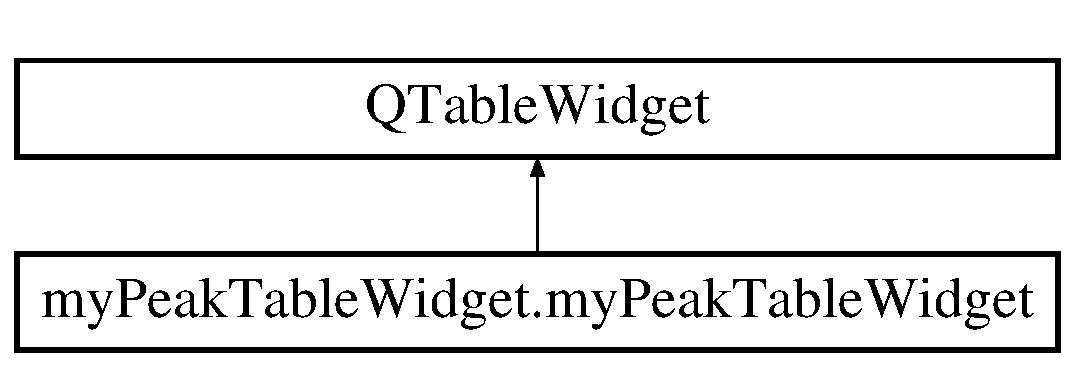
\includegraphics[height=2.000000cm]{classmy_peak_table_widget_1_1my_peak_table_widget}
\end{center}
\end{figure}
\subsection*{Public Member Functions}
\begin{DoxyCompactItemize}
\item 
def \hyperlink{classmy_peak_table_widget_1_1my_peak_table_widget_a112e9c9fe94f89bee7313906355d6c8f}{\-\_\-\-\_\-init\-\_\-\-\_\-}
\item 
def \hyperlink{classmy_peak_table_widget_1_1my_peak_table_widget_abc9980e6816ae93b1302da488b1eb83b}{set\-Image\-File\-Name}
\item 
def \hyperlink{classmy_peak_table_widget_1_1my_peak_table_widget_a30d9b900b3a8eb5fac45aacdd1355b4c}{set\-Detector}
\item 
def \hyperlink{classmy_peak_table_widget_1_1my_peak_table_widget_a3c7bc1e38db2eb6e0458a438a753f6c3}{set\-Peaks}
\item 
def \hyperlink{classmy_peak_table_widget_1_1my_peak_table_widget_aa4aed89efa31348e87d73f711d996daf}{add\-Peak}
\item 
def \hyperlink{classmy_peak_table_widget_1_1my_peak_table_widget_ac06c362f6d4a47181fbcc0fe2e78a2cb}{peak\-Edit}
\end{DoxyCompactItemize}
\subsection*{Public Attributes}
\begin{DoxyCompactItemize}
\item 
\hyperlink{classmy_peak_table_widget_1_1my_peak_table_widget_ac482a5f93ba7061a3a6e8c6d46e2e26b}{imfile}
\item 
\hyperlink{classmy_peak_table_widget_1_1my_peak_table_widget_a9c8259e29d4d739d45452eaec8bebff0}{my\-Det}
\item 
\hyperlink{classmy_peak_table_widget_1_1my_peak_table_widget_afa4b43bf4a5bf3308bf8a7d4c146712b}{peaks}
\item 
\hyperlink{classmy_peak_table_widget_1_1my_peak_table_widget_ae4934e86392397c16937ababde3ac38e}{num\-Peaks}
\end{DoxyCompactItemize}
\subsection*{Static Public Attributes}
\begin{DoxyCompactItemize}
\item 
int \hyperlink{classmy_peak_table_widget_1_1my_peak_table_widget_a8e630a6f15d224300abc621b8bac8e23}{num\-Peaks} = 0
\item 
tuple \hyperlink{classmy_peak_table_widget_1_1my_peak_table_widget_a6b0c16aabbedcc000d20542e5d4b3e08}{head\-List} = Qt\-Core.\-Q\-String(\char`\"{}X;Y;2-\/theta;d-\/spacing;h;k;l;rot. angle\char`\"{})
\item 
int \hyperlink{classmy_peak_table_widget_1_1my_peak_table_widget_a7be636c918a7d4e642015b4531795477}{my\-Det} = 0
\item 
int \hyperlink{classmy_peak_table_widget_1_1my_peak_table_widget_a00a3801ee16f8bb1b140b254793e098c}{peaks} = 0
\item 
string \hyperlink{classmy_peak_table_widget_1_1my_peak_table_widget_ae072cce7f45a7c9a7c4a4d6ea9887593}{imname} = ''
\end{DoxyCompactItemize}


\subsection{Constructor \& Destructor Documentation}
\hypertarget{classmy_peak_table_widget_1_1my_peak_table_widget_a112e9c9fe94f89bee7313906355d6c8f}{\index{my\-Peak\-Table\-Widget\-::my\-Peak\-Table\-Widget@{my\-Peak\-Table\-Widget\-::my\-Peak\-Table\-Widget}!\-\_\-\-\_\-init\-\_\-\-\_\-@{\-\_\-\-\_\-init\-\_\-\-\_\-}}
\index{\-\_\-\-\_\-init\-\_\-\-\_\-@{\-\_\-\-\_\-init\-\_\-\-\_\-}!myPeakTableWidget::myPeakTableWidget@{my\-Peak\-Table\-Widget\-::my\-Peak\-Table\-Widget}}
\subsubsection[{\-\_\-\-\_\-init\-\_\-\-\_\-}]{\setlength{\rightskip}{0pt plus 5cm}def my\-Peak\-Table\-Widget.\-my\-Peak\-Table\-Widget.\-\_\-\-\_\-init\-\_\-\-\_\- (
\begin{DoxyParamCaption}
\item[{}]{self, }
\item[{}]{parent = {\ttfamily None}}
\end{DoxyParamCaption}
)}}\label{classmy_peak_table_widget_1_1my_peak_table_widget_a112e9c9fe94f89bee7313906355d6c8f}


\subsection{Member Function Documentation}
\hypertarget{classmy_peak_table_widget_1_1my_peak_table_widget_aa4aed89efa31348e87d73f711d996daf}{\index{my\-Peak\-Table\-Widget\-::my\-Peak\-Table\-Widget@{my\-Peak\-Table\-Widget\-::my\-Peak\-Table\-Widget}!add\-Peak@{add\-Peak}}
\index{add\-Peak@{add\-Peak}!myPeakTableWidget::myPeakTableWidget@{my\-Peak\-Table\-Widget\-::my\-Peak\-Table\-Widget}}
\subsubsection[{add\-Peak}]{\setlength{\rightskip}{0pt plus 5cm}def my\-Peak\-Table\-Widget.\-my\-Peak\-Table\-Widget.\-add\-Peak (
\begin{DoxyParamCaption}
\item[{}]{self, }
\item[{}]{peak}
\end{DoxyParamCaption}
)}}\label{classmy_peak_table_widget_1_1my_peak_table_widget_aa4aed89efa31348e87d73f711d996daf}
\hypertarget{classmy_peak_table_widget_1_1my_peak_table_widget_ac06c362f6d4a47181fbcc0fe2e78a2cb}{\index{my\-Peak\-Table\-Widget\-::my\-Peak\-Table\-Widget@{my\-Peak\-Table\-Widget\-::my\-Peak\-Table\-Widget}!peak\-Edit@{peak\-Edit}}
\index{peak\-Edit@{peak\-Edit}!myPeakTableWidget::myPeakTableWidget@{my\-Peak\-Table\-Widget\-::my\-Peak\-Table\-Widget}}
\subsubsection[{peak\-Edit}]{\setlength{\rightskip}{0pt plus 5cm}def my\-Peak\-Table\-Widget.\-my\-Peak\-Table\-Widget.\-peak\-Edit (
\begin{DoxyParamCaption}
\item[{}]{self, }
\item[{}]{row, }
\item[{}]{col}
\end{DoxyParamCaption}
)}}\label{classmy_peak_table_widget_1_1my_peak_table_widget_ac06c362f6d4a47181fbcc0fe2e78a2cb}
\hypertarget{classmy_peak_table_widget_1_1my_peak_table_widget_a30d9b900b3a8eb5fac45aacdd1355b4c}{\index{my\-Peak\-Table\-Widget\-::my\-Peak\-Table\-Widget@{my\-Peak\-Table\-Widget\-::my\-Peak\-Table\-Widget}!set\-Detector@{set\-Detector}}
\index{set\-Detector@{set\-Detector}!myPeakTableWidget::myPeakTableWidget@{my\-Peak\-Table\-Widget\-::my\-Peak\-Table\-Widget}}
\subsubsection[{set\-Detector}]{\setlength{\rightskip}{0pt plus 5cm}def my\-Peak\-Table\-Widget.\-my\-Peak\-Table\-Widget.\-set\-Detector (
\begin{DoxyParamCaption}
\item[{}]{self, }
\item[{}]{det}
\end{DoxyParamCaption}
)}}\label{classmy_peak_table_widget_1_1my_peak_table_widget_a30d9b900b3a8eb5fac45aacdd1355b4c}
\hypertarget{classmy_peak_table_widget_1_1my_peak_table_widget_abc9980e6816ae93b1302da488b1eb83b}{\index{my\-Peak\-Table\-Widget\-::my\-Peak\-Table\-Widget@{my\-Peak\-Table\-Widget\-::my\-Peak\-Table\-Widget}!set\-Image\-File\-Name@{set\-Image\-File\-Name}}
\index{set\-Image\-File\-Name@{set\-Image\-File\-Name}!myPeakTableWidget::myPeakTableWidget@{my\-Peak\-Table\-Widget\-::my\-Peak\-Table\-Widget}}
\subsubsection[{set\-Image\-File\-Name}]{\setlength{\rightskip}{0pt plus 5cm}def my\-Peak\-Table\-Widget.\-my\-Peak\-Table\-Widget.\-set\-Image\-File\-Name (
\begin{DoxyParamCaption}
\item[{}]{self, }
\item[{}]{imname}
\end{DoxyParamCaption}
)}}\label{classmy_peak_table_widget_1_1my_peak_table_widget_abc9980e6816ae93b1302da488b1eb83b}
\hypertarget{classmy_peak_table_widget_1_1my_peak_table_widget_a3c7bc1e38db2eb6e0458a438a753f6c3}{\index{my\-Peak\-Table\-Widget\-::my\-Peak\-Table\-Widget@{my\-Peak\-Table\-Widget\-::my\-Peak\-Table\-Widget}!set\-Peaks@{set\-Peaks}}
\index{set\-Peaks@{set\-Peaks}!myPeakTableWidget::myPeakTableWidget@{my\-Peak\-Table\-Widget\-::my\-Peak\-Table\-Widget}}
\subsubsection[{set\-Peaks}]{\setlength{\rightskip}{0pt plus 5cm}def my\-Peak\-Table\-Widget.\-my\-Peak\-Table\-Widget.\-set\-Peaks (
\begin{DoxyParamCaption}
\item[{}]{self, }
\item[{}]{peaks}
\end{DoxyParamCaption}
)}}\label{classmy_peak_table_widget_1_1my_peak_table_widget_a3c7bc1e38db2eb6e0458a438a753f6c3}


\subsection{Member Data Documentation}
\hypertarget{classmy_peak_table_widget_1_1my_peak_table_widget_a6b0c16aabbedcc000d20542e5d4b3e08}{\index{my\-Peak\-Table\-Widget\-::my\-Peak\-Table\-Widget@{my\-Peak\-Table\-Widget\-::my\-Peak\-Table\-Widget}!head\-List@{head\-List}}
\index{head\-List@{head\-List}!myPeakTableWidget::myPeakTableWidget@{my\-Peak\-Table\-Widget\-::my\-Peak\-Table\-Widget}}
\subsubsection[{head\-List}]{\setlength{\rightskip}{0pt plus 5cm}tuple my\-Peak\-Table\-Widget.\-my\-Peak\-Table\-Widget.\-head\-List = Qt\-Core.\-Q\-String(\char`\"{}X;Y;2-\/theta;d-\/spacing;h;k;l;rot. angle\char`\"{})\hspace{0.3cm}{\ttfamily [static]}}}\label{classmy_peak_table_widget_1_1my_peak_table_widget_a6b0c16aabbedcc000d20542e5d4b3e08}
\hypertarget{classmy_peak_table_widget_1_1my_peak_table_widget_ac482a5f93ba7061a3a6e8c6d46e2e26b}{\index{my\-Peak\-Table\-Widget\-::my\-Peak\-Table\-Widget@{my\-Peak\-Table\-Widget\-::my\-Peak\-Table\-Widget}!imfile@{imfile}}
\index{imfile@{imfile}!myPeakTableWidget::myPeakTableWidget@{my\-Peak\-Table\-Widget\-::my\-Peak\-Table\-Widget}}
\subsubsection[{imfile}]{\setlength{\rightskip}{0pt plus 5cm}my\-Peak\-Table\-Widget.\-my\-Peak\-Table\-Widget.\-imfile}}\label{classmy_peak_table_widget_1_1my_peak_table_widget_ac482a5f93ba7061a3a6e8c6d46e2e26b}
\hypertarget{classmy_peak_table_widget_1_1my_peak_table_widget_ae072cce7f45a7c9a7c4a4d6ea9887593}{\index{my\-Peak\-Table\-Widget\-::my\-Peak\-Table\-Widget@{my\-Peak\-Table\-Widget\-::my\-Peak\-Table\-Widget}!imname@{imname}}
\index{imname@{imname}!myPeakTableWidget::myPeakTableWidget@{my\-Peak\-Table\-Widget\-::my\-Peak\-Table\-Widget}}
\subsubsection[{imname}]{\setlength{\rightskip}{0pt plus 5cm}string my\-Peak\-Table\-Widget.\-my\-Peak\-Table\-Widget.\-imname = ''\hspace{0.3cm}{\ttfamily [static]}}}\label{classmy_peak_table_widget_1_1my_peak_table_widget_ae072cce7f45a7c9a7c4a4d6ea9887593}
\hypertarget{classmy_peak_table_widget_1_1my_peak_table_widget_a7be636c918a7d4e642015b4531795477}{\index{my\-Peak\-Table\-Widget\-::my\-Peak\-Table\-Widget@{my\-Peak\-Table\-Widget\-::my\-Peak\-Table\-Widget}!my\-Det@{my\-Det}}
\index{my\-Det@{my\-Det}!myPeakTableWidget::myPeakTableWidget@{my\-Peak\-Table\-Widget\-::my\-Peak\-Table\-Widget}}
\subsubsection[{my\-Det}]{\setlength{\rightskip}{0pt plus 5cm}int my\-Peak\-Table\-Widget.\-my\-Peak\-Table\-Widget.\-my\-Det = 0\hspace{0.3cm}{\ttfamily [static]}}}\label{classmy_peak_table_widget_1_1my_peak_table_widget_a7be636c918a7d4e642015b4531795477}
\hypertarget{classmy_peak_table_widget_1_1my_peak_table_widget_a9c8259e29d4d739d45452eaec8bebff0}{\index{my\-Peak\-Table\-Widget\-::my\-Peak\-Table\-Widget@{my\-Peak\-Table\-Widget\-::my\-Peak\-Table\-Widget}!my\-Det@{my\-Det}}
\index{my\-Det@{my\-Det}!myPeakTableWidget::myPeakTableWidget@{my\-Peak\-Table\-Widget\-::my\-Peak\-Table\-Widget}}
\subsubsection[{my\-Det}]{\setlength{\rightskip}{0pt plus 5cm}my\-Peak\-Table\-Widget.\-my\-Peak\-Table\-Widget.\-my\-Det}}\label{classmy_peak_table_widget_1_1my_peak_table_widget_a9c8259e29d4d739d45452eaec8bebff0}
\hypertarget{classmy_peak_table_widget_1_1my_peak_table_widget_a8e630a6f15d224300abc621b8bac8e23}{\index{my\-Peak\-Table\-Widget\-::my\-Peak\-Table\-Widget@{my\-Peak\-Table\-Widget\-::my\-Peak\-Table\-Widget}!num\-Peaks@{num\-Peaks}}
\index{num\-Peaks@{num\-Peaks}!myPeakTableWidget::myPeakTableWidget@{my\-Peak\-Table\-Widget\-::my\-Peak\-Table\-Widget}}
\subsubsection[{num\-Peaks}]{\setlength{\rightskip}{0pt plus 5cm}int my\-Peak\-Table\-Widget.\-my\-Peak\-Table\-Widget.\-num\-Peaks = 0\hspace{0.3cm}{\ttfamily [static]}}}\label{classmy_peak_table_widget_1_1my_peak_table_widget_a8e630a6f15d224300abc621b8bac8e23}
\hypertarget{classmy_peak_table_widget_1_1my_peak_table_widget_ae4934e86392397c16937ababde3ac38e}{\index{my\-Peak\-Table\-Widget\-::my\-Peak\-Table\-Widget@{my\-Peak\-Table\-Widget\-::my\-Peak\-Table\-Widget}!num\-Peaks@{num\-Peaks}}
\index{num\-Peaks@{num\-Peaks}!myPeakTableWidget::myPeakTableWidget@{my\-Peak\-Table\-Widget\-::my\-Peak\-Table\-Widget}}
\subsubsection[{num\-Peaks}]{\setlength{\rightskip}{0pt plus 5cm}my\-Peak\-Table\-Widget.\-my\-Peak\-Table\-Widget.\-num\-Peaks}}\label{classmy_peak_table_widget_1_1my_peak_table_widget_ae4934e86392397c16937ababde3ac38e}
\hypertarget{classmy_peak_table_widget_1_1my_peak_table_widget_a00a3801ee16f8bb1b140b254793e098c}{\index{my\-Peak\-Table\-Widget\-::my\-Peak\-Table\-Widget@{my\-Peak\-Table\-Widget\-::my\-Peak\-Table\-Widget}!peaks@{peaks}}
\index{peaks@{peaks}!myPeakTableWidget::myPeakTableWidget@{my\-Peak\-Table\-Widget\-::my\-Peak\-Table\-Widget}}
\subsubsection[{peaks}]{\setlength{\rightskip}{0pt plus 5cm}int my\-Peak\-Table\-Widget.\-my\-Peak\-Table\-Widget.\-peaks = 0\hspace{0.3cm}{\ttfamily [static]}}}\label{classmy_peak_table_widget_1_1my_peak_table_widget_a00a3801ee16f8bb1b140b254793e098c}
\hypertarget{classmy_peak_table_widget_1_1my_peak_table_widget_afa4b43bf4a5bf3308bf8a7d4c146712b}{\index{my\-Peak\-Table\-Widget\-::my\-Peak\-Table\-Widget@{my\-Peak\-Table\-Widget\-::my\-Peak\-Table\-Widget}!peaks@{peaks}}
\index{peaks@{peaks}!myPeakTableWidget::myPeakTableWidget@{my\-Peak\-Table\-Widget\-::my\-Peak\-Table\-Widget}}
\subsubsection[{peaks}]{\setlength{\rightskip}{0pt plus 5cm}my\-Peak\-Table\-Widget.\-my\-Peak\-Table\-Widget.\-peaks}}\label{classmy_peak_table_widget_1_1my_peak_table_widget_afa4b43bf4a5bf3308bf8a7d4c146712b}


The documentation for this class was generated from the following file\-:\begin{DoxyCompactItemize}
\item 
workdir/atrex/\-Software/\hyperlink{my_peak_table_widget_8py}{my\-Peak\-Table\-Widget.\-py}\end{DoxyCompactItemize}

\hypertarget{class_my_plot_widget_1_1_my_plot_widget}{\section{My\-Plot\-Widget.\-My\-Plot\-Widget Class Reference}
\label{class_my_plot_widget_1_1_my_plot_widget}\index{My\-Plot\-Widget.\-My\-Plot\-Widget@{My\-Plot\-Widget.\-My\-Plot\-Widget}}
}
Inheritance diagram for My\-Plot\-Widget.\-My\-Plot\-Widget\-:\begin{figure}[H]
\begin{center}
\leavevmode
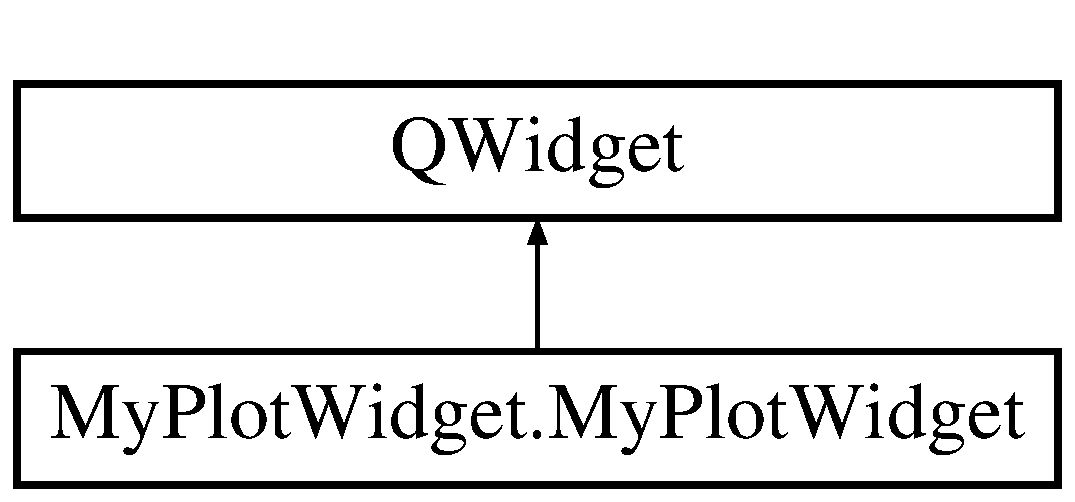
\includegraphics[height=2.000000cm]{class_my_plot_widget_1_1_my_plot_widget}
\end{center}
\end{figure}
\subsection*{Public Member Functions}
\begin{DoxyCompactItemize}
\item 
def \hyperlink{class_my_plot_widget_1_1_my_plot_widget_a6609ab444ac92ada3d856756c4d63ff3}{\-\_\-\-\_\-init\-\_\-\-\_\-}
\item 
def \hyperlink{class_my_plot_widget_1_1_my_plot_widget_a7cc35e9fdcea629d444e69c9be1f17e5}{size\-Hint}
\item 
def \hyperlink{class_my_plot_widget_1_1_my_plot_widget_a24bbe5fb4b29afdb328e65616fd49607}{minimum\-Size\-Hint}
\item 
def \hyperlink{class_my_plot_widget_1_1_my_plot_widget_a51f5c70ea2dd4024e4c56a0a73925164}{plot\-Data}
\item 
def \hyperlink{class_my_plot_widget_1_1_my_plot_widget_aa715ad5a13d60bef1d1d8f35d17a128d}{plot\-Data\-X\-Y2}
\item 
def \hyperlink{class_my_plot_widget_1_1_my_plot_widget_adf3455693401acc7a41cc2b167c8ea7d}{set\-X\-Y\-Data}
\item 
def \hyperlink{class_my_plot_widget_1_1_my_plot_widget_a6298a336d89650749a4c04e28bcf4274}{set\-Overlay\-X\-Y\-Data}
\item 
def \hyperlink{class_my_plot_widget_1_1_my_plot_widget_ac55f01d08b5bf74fe1bfeb2719747a92}{set\-X\-Y\-Data\-\_\-\-Integrate}
\item 
def \hyperlink{class_my_plot_widget_1_1_my_plot_widget_a2ba64fd7e8dd68a755267f4fbcde2b45}{create\-Cos\-Data}
\item 
def \hyperlink{class_my_plot_widget_1_1_my_plot_widget_a866f749621b291e90310593be2c612f8}{setp\-Type}
\item 
def \hyperlink{class_my_plot_widget_1_1_my_plot_widget_a9363485b431a40f93626e21842248589}{set\-Labels}
\item 
def \hyperlink{class_my_plot_widget_1_1_my_plot_widget_ae782a56a3f86e3e4a7c57fcc3ab55fa7}{output\-To\-File}
\end{DoxyCompactItemize}
\subsection*{Public Attributes}
\begin{DoxyCompactItemize}
\item 
\hyperlink{class_my_plot_widget_1_1_my_plot_widget_a3f90de6f5ac0f2f681457c7d1db66422}{figure}
\item 
\hyperlink{class_my_plot_widget_1_1_my_plot_widget_ae40a5f04a117f5863db217e6134cde3a}{canvas}
\item 
\hyperlink{class_my_plot_widget_1_1_my_plot_widget_a5c0d1b439e1708a9e105e9c1123ba19c}{toolbar}
\item 
\hyperlink{class_my_plot_widget_1_1_my_plot_widget_afdd3a63e478b90f8a9d43d813eef44f3}{axes}
\item 
\hyperlink{class_my_plot_widget_1_1_my_plot_widget_a4a63c84c067d764fcdef1e84b36331a4}{p\-Type}
\item 
\hyperlink{class_my_plot_widget_1_1_my_plot_widget_a1ca45f1c4b0bea8328ca2926126f0468}{tstr}
\item 
\hyperlink{class_my_plot_widget_1_1_my_plot_widget_a07aaae96f1d5667f6125cf6bf7274a14}{xstr}
\item 
\hyperlink{class_my_plot_widget_1_1_my_plot_widget_a1257bc7678d216ec50d9cafa6329c8a7}{ystr}
\item 
\hyperlink{class_my_plot_widget_1_1_my_plot_widget_aa95c6b8ff2b9952b5f4fdca6b5aa2901}{olay\-Flag}
\item 
\hyperlink{class_my_plot_widget_1_1_my_plot_widget_a64e693fbacbde23a8c8d08899aa6dcdd}{plot\-Data\-Flag}
\item 
\hyperlink{class_my_plot_widget_1_1_my_plot_widget_af8e35141d9588e42805da0c06bcffd32}{xarr}
\item 
\hyperlink{class_my_plot_widget_1_1_my_plot_widget_aa1b1b70359cb0139710db0982040778b}{yarr}
\item 
\hyperlink{class_my_plot_widget_1_1_my_plot_widget_ada9f240a51b2615a25fef530c4028350}{x10}
\item 
\hyperlink{class_my_plot_widget_1_1_my_plot_widget_a2bcd4bfd7b9d5c75e58140845b87508d}{yarr\-Spline}
\item 
\hyperlink{class_my_plot_widget_1_1_my_plot_widget_ad4ac85f27d3aded8658bb61a50c3f72e}{xarr\-Olay}
\item 
\hyperlink{class_my_plot_widget_1_1_my_plot_widget_a26308ed5767dd716db3984aa549fddef}{yarr\-Olay}
\end{DoxyCompactItemize}


\subsection{Constructor \& Destructor Documentation}
\hypertarget{class_my_plot_widget_1_1_my_plot_widget_a6609ab444ac92ada3d856756c4d63ff3}{\index{My\-Plot\-Widget\-::\-My\-Plot\-Widget@{My\-Plot\-Widget\-::\-My\-Plot\-Widget}!\-\_\-\-\_\-init\-\_\-\-\_\-@{\-\_\-\-\_\-init\-\_\-\-\_\-}}
\index{\-\_\-\-\_\-init\-\_\-\-\_\-@{\-\_\-\-\_\-init\-\_\-\-\_\-}!MyPlotWidget::MyPlotWidget@{My\-Plot\-Widget\-::\-My\-Plot\-Widget}}
\subsubsection[{\-\_\-\-\_\-init\-\_\-\-\_\-}]{\setlength{\rightskip}{0pt plus 5cm}def My\-Plot\-Widget.\-My\-Plot\-Widget.\-\_\-\-\_\-init\-\_\-\-\_\- (
\begin{DoxyParamCaption}
\item[{}]{self, }
\item[{}]{parent}
\end{DoxyParamCaption}
)}}\label{class_my_plot_widget_1_1_my_plot_widget_a6609ab444ac92ada3d856756c4d63ff3}


\subsection{Member Function Documentation}
\hypertarget{class_my_plot_widget_1_1_my_plot_widget_a2ba64fd7e8dd68a755267f4fbcde2b45}{\index{My\-Plot\-Widget\-::\-My\-Plot\-Widget@{My\-Plot\-Widget\-::\-My\-Plot\-Widget}!create\-Cos\-Data@{create\-Cos\-Data}}
\index{create\-Cos\-Data@{create\-Cos\-Data}!MyPlotWidget::MyPlotWidget@{My\-Plot\-Widget\-::\-My\-Plot\-Widget}}
\subsubsection[{create\-Cos\-Data}]{\setlength{\rightskip}{0pt plus 5cm}def My\-Plot\-Widget.\-My\-Plot\-Widget.\-create\-Cos\-Data (
\begin{DoxyParamCaption}
\item[{}]{self}
\end{DoxyParamCaption}
)}}\label{class_my_plot_widget_1_1_my_plot_widget_a2ba64fd7e8dd68a755267f4fbcde2b45}
\hypertarget{class_my_plot_widget_1_1_my_plot_widget_a24bbe5fb4b29afdb328e65616fd49607}{\index{My\-Plot\-Widget\-::\-My\-Plot\-Widget@{My\-Plot\-Widget\-::\-My\-Plot\-Widget}!minimum\-Size\-Hint@{minimum\-Size\-Hint}}
\index{minimum\-Size\-Hint@{minimum\-Size\-Hint}!MyPlotWidget::MyPlotWidget@{My\-Plot\-Widget\-::\-My\-Plot\-Widget}}
\subsubsection[{minimum\-Size\-Hint}]{\setlength{\rightskip}{0pt plus 5cm}def My\-Plot\-Widget.\-My\-Plot\-Widget.\-minimum\-Size\-Hint (
\begin{DoxyParamCaption}
\item[{}]{self}
\end{DoxyParamCaption}
)}}\label{class_my_plot_widget_1_1_my_plot_widget_a24bbe5fb4b29afdb328e65616fd49607}
\hypertarget{class_my_plot_widget_1_1_my_plot_widget_ae782a56a3f86e3e4a7c57fcc3ab55fa7}{\index{My\-Plot\-Widget\-::\-My\-Plot\-Widget@{My\-Plot\-Widget\-::\-My\-Plot\-Widget}!output\-To\-File@{output\-To\-File}}
\index{output\-To\-File@{output\-To\-File}!MyPlotWidget::MyPlotWidget@{My\-Plot\-Widget\-::\-My\-Plot\-Widget}}
\subsubsection[{output\-To\-File}]{\setlength{\rightskip}{0pt plus 5cm}def My\-Plot\-Widget.\-My\-Plot\-Widget.\-output\-To\-File (
\begin{DoxyParamCaption}
\item[{}]{self, }
\item[{}]{fname}
\end{DoxyParamCaption}
)}}\label{class_my_plot_widget_1_1_my_plot_widget_ae782a56a3f86e3e4a7c57fcc3ab55fa7}
\hypertarget{class_my_plot_widget_1_1_my_plot_widget_a51f5c70ea2dd4024e4c56a0a73925164}{\index{My\-Plot\-Widget\-::\-My\-Plot\-Widget@{My\-Plot\-Widget\-::\-My\-Plot\-Widget}!plot\-Data@{plot\-Data}}
\index{plot\-Data@{plot\-Data}!MyPlotWidget::MyPlotWidget@{My\-Plot\-Widget\-::\-My\-Plot\-Widget}}
\subsubsection[{plot\-Data}]{\setlength{\rightskip}{0pt plus 5cm}def My\-Plot\-Widget.\-My\-Plot\-Widget.\-plot\-Data (
\begin{DoxyParamCaption}
\item[{}]{self}
\end{DoxyParamCaption}
)}}\label{class_my_plot_widget_1_1_my_plot_widget_a51f5c70ea2dd4024e4c56a0a73925164}
\hypertarget{class_my_plot_widget_1_1_my_plot_widget_aa715ad5a13d60bef1d1d8f35d17a128d}{\index{My\-Plot\-Widget\-::\-My\-Plot\-Widget@{My\-Plot\-Widget\-::\-My\-Plot\-Widget}!plot\-Data\-X\-Y2@{plot\-Data\-X\-Y2}}
\index{plot\-Data\-X\-Y2@{plot\-Data\-X\-Y2}!MyPlotWidget::MyPlotWidget@{My\-Plot\-Widget\-::\-My\-Plot\-Widget}}
\subsubsection[{plot\-Data\-X\-Y2}]{\setlength{\rightskip}{0pt plus 5cm}def My\-Plot\-Widget.\-My\-Plot\-Widget.\-plot\-Data\-X\-Y2 (
\begin{DoxyParamCaption}
\item[{}]{self, }
\item[{}]{xarr, }
\item[{}]{yarr, }
\item[{}]{yarr\-Fit}
\end{DoxyParamCaption}
)}}\label{class_my_plot_widget_1_1_my_plot_widget_aa715ad5a13d60bef1d1d8f35d17a128d}
\hypertarget{class_my_plot_widget_1_1_my_plot_widget_a9363485b431a40f93626e21842248589}{\index{My\-Plot\-Widget\-::\-My\-Plot\-Widget@{My\-Plot\-Widget\-::\-My\-Plot\-Widget}!set\-Labels@{set\-Labels}}
\index{set\-Labels@{set\-Labels}!MyPlotWidget::MyPlotWidget@{My\-Plot\-Widget\-::\-My\-Plot\-Widget}}
\subsubsection[{set\-Labels}]{\setlength{\rightskip}{0pt plus 5cm}def My\-Plot\-Widget.\-My\-Plot\-Widget.\-set\-Labels (
\begin{DoxyParamCaption}
\item[{}]{self, }
\item[{}]{title\-String, }
\item[{}]{x\-String, }
\item[{}]{y\-String}
\end{DoxyParamCaption}
)}}\label{class_my_plot_widget_1_1_my_plot_widget_a9363485b431a40f93626e21842248589}
\hypertarget{class_my_plot_widget_1_1_my_plot_widget_a6298a336d89650749a4c04e28bcf4274}{\index{My\-Plot\-Widget\-::\-My\-Plot\-Widget@{My\-Plot\-Widget\-::\-My\-Plot\-Widget}!set\-Overlay\-X\-Y\-Data@{set\-Overlay\-X\-Y\-Data}}
\index{set\-Overlay\-X\-Y\-Data@{set\-Overlay\-X\-Y\-Data}!MyPlotWidget::MyPlotWidget@{My\-Plot\-Widget\-::\-My\-Plot\-Widget}}
\subsubsection[{set\-Overlay\-X\-Y\-Data}]{\setlength{\rightskip}{0pt plus 5cm}def My\-Plot\-Widget.\-My\-Plot\-Widget.\-set\-Overlay\-X\-Y\-Data (
\begin{DoxyParamCaption}
\item[{}]{self, }
\item[{}]{xarr, }
\item[{}]{yarr, }
\item[{}]{sec\-Flag}
\end{DoxyParamCaption}
)}}\label{class_my_plot_widget_1_1_my_plot_widget_a6298a336d89650749a4c04e28bcf4274}
\hypertarget{class_my_plot_widget_1_1_my_plot_widget_a866f749621b291e90310593be2c612f8}{\index{My\-Plot\-Widget\-::\-My\-Plot\-Widget@{My\-Plot\-Widget\-::\-My\-Plot\-Widget}!setp\-Type@{setp\-Type}}
\index{setp\-Type@{setp\-Type}!MyPlotWidget::MyPlotWidget@{My\-Plot\-Widget\-::\-My\-Plot\-Widget}}
\subsubsection[{setp\-Type}]{\setlength{\rightskip}{0pt plus 5cm}def My\-Plot\-Widget.\-My\-Plot\-Widget.\-setp\-Type (
\begin{DoxyParamCaption}
\item[{}]{self, }
\item[{}]{type}
\end{DoxyParamCaption}
)}}\label{class_my_plot_widget_1_1_my_plot_widget_a866f749621b291e90310593be2c612f8}
\hypertarget{class_my_plot_widget_1_1_my_plot_widget_adf3455693401acc7a41cc2b167c8ea7d}{\index{My\-Plot\-Widget\-::\-My\-Plot\-Widget@{My\-Plot\-Widget\-::\-My\-Plot\-Widget}!set\-X\-Y\-Data@{set\-X\-Y\-Data}}
\index{set\-X\-Y\-Data@{set\-X\-Y\-Data}!MyPlotWidget::MyPlotWidget@{My\-Plot\-Widget\-::\-My\-Plot\-Widget}}
\subsubsection[{set\-X\-Y\-Data}]{\setlength{\rightskip}{0pt plus 5cm}def My\-Plot\-Widget.\-My\-Plot\-Widget.\-set\-X\-Y\-Data (
\begin{DoxyParamCaption}
\item[{}]{self, }
\item[{}]{xarr, }
\item[{}]{yarr}
\end{DoxyParamCaption}
)}}\label{class_my_plot_widget_1_1_my_plot_widget_adf3455693401acc7a41cc2b167c8ea7d}
\hypertarget{class_my_plot_widget_1_1_my_plot_widget_ac55f01d08b5bf74fe1bfeb2719747a92}{\index{My\-Plot\-Widget\-::\-My\-Plot\-Widget@{My\-Plot\-Widget\-::\-My\-Plot\-Widget}!set\-X\-Y\-Data\-\_\-\-Integrate@{set\-X\-Y\-Data\-\_\-\-Integrate}}
\index{set\-X\-Y\-Data\-\_\-\-Integrate@{set\-X\-Y\-Data\-\_\-\-Integrate}!MyPlotWidget::MyPlotWidget@{My\-Plot\-Widget\-::\-My\-Plot\-Widget}}
\subsubsection[{set\-X\-Y\-Data\-\_\-\-Integrate}]{\setlength{\rightskip}{0pt plus 5cm}def My\-Plot\-Widget.\-My\-Plot\-Widget.\-set\-X\-Y\-Data\-\_\-\-Integrate (
\begin{DoxyParamCaption}
\item[{}]{self, }
\item[{}]{xarr, }
\item[{}]{yarr}
\end{DoxyParamCaption}
)}}\label{class_my_plot_widget_1_1_my_plot_widget_ac55f01d08b5bf74fe1bfeb2719747a92}
\hypertarget{class_my_plot_widget_1_1_my_plot_widget_a7cc35e9fdcea629d444e69c9be1f17e5}{\index{My\-Plot\-Widget\-::\-My\-Plot\-Widget@{My\-Plot\-Widget\-::\-My\-Plot\-Widget}!size\-Hint@{size\-Hint}}
\index{size\-Hint@{size\-Hint}!MyPlotWidget::MyPlotWidget@{My\-Plot\-Widget\-::\-My\-Plot\-Widget}}
\subsubsection[{size\-Hint}]{\setlength{\rightskip}{0pt plus 5cm}def My\-Plot\-Widget.\-My\-Plot\-Widget.\-size\-Hint (
\begin{DoxyParamCaption}
\item[{}]{self}
\end{DoxyParamCaption}
)}}\label{class_my_plot_widget_1_1_my_plot_widget_a7cc35e9fdcea629d444e69c9be1f17e5}


\subsection{Member Data Documentation}
\hypertarget{class_my_plot_widget_1_1_my_plot_widget_afdd3a63e478b90f8a9d43d813eef44f3}{\index{My\-Plot\-Widget\-::\-My\-Plot\-Widget@{My\-Plot\-Widget\-::\-My\-Plot\-Widget}!axes@{axes}}
\index{axes@{axes}!MyPlotWidget::MyPlotWidget@{My\-Plot\-Widget\-::\-My\-Plot\-Widget}}
\subsubsection[{axes}]{\setlength{\rightskip}{0pt plus 5cm}My\-Plot\-Widget.\-My\-Plot\-Widget.\-axes}}\label{class_my_plot_widget_1_1_my_plot_widget_afdd3a63e478b90f8a9d43d813eef44f3}
\hypertarget{class_my_plot_widget_1_1_my_plot_widget_ae40a5f04a117f5863db217e6134cde3a}{\index{My\-Plot\-Widget\-::\-My\-Plot\-Widget@{My\-Plot\-Widget\-::\-My\-Plot\-Widget}!canvas@{canvas}}
\index{canvas@{canvas}!MyPlotWidget::MyPlotWidget@{My\-Plot\-Widget\-::\-My\-Plot\-Widget}}
\subsubsection[{canvas}]{\setlength{\rightskip}{0pt plus 5cm}My\-Plot\-Widget.\-My\-Plot\-Widget.\-canvas}}\label{class_my_plot_widget_1_1_my_plot_widget_ae40a5f04a117f5863db217e6134cde3a}
\hypertarget{class_my_plot_widget_1_1_my_plot_widget_a3f90de6f5ac0f2f681457c7d1db66422}{\index{My\-Plot\-Widget\-::\-My\-Plot\-Widget@{My\-Plot\-Widget\-::\-My\-Plot\-Widget}!figure@{figure}}
\index{figure@{figure}!MyPlotWidget::MyPlotWidget@{My\-Plot\-Widget\-::\-My\-Plot\-Widget}}
\subsubsection[{figure}]{\setlength{\rightskip}{0pt plus 5cm}My\-Plot\-Widget.\-My\-Plot\-Widget.\-figure}}\label{class_my_plot_widget_1_1_my_plot_widget_a3f90de6f5ac0f2f681457c7d1db66422}
\hypertarget{class_my_plot_widget_1_1_my_plot_widget_aa95c6b8ff2b9952b5f4fdca6b5aa2901}{\index{My\-Plot\-Widget\-::\-My\-Plot\-Widget@{My\-Plot\-Widget\-::\-My\-Plot\-Widget}!olay\-Flag@{olay\-Flag}}
\index{olay\-Flag@{olay\-Flag}!MyPlotWidget::MyPlotWidget@{My\-Plot\-Widget\-::\-My\-Plot\-Widget}}
\subsubsection[{olay\-Flag}]{\setlength{\rightskip}{0pt plus 5cm}My\-Plot\-Widget.\-My\-Plot\-Widget.\-olay\-Flag}}\label{class_my_plot_widget_1_1_my_plot_widget_aa95c6b8ff2b9952b5f4fdca6b5aa2901}
\hypertarget{class_my_plot_widget_1_1_my_plot_widget_a64e693fbacbde23a8c8d08899aa6dcdd}{\index{My\-Plot\-Widget\-::\-My\-Plot\-Widget@{My\-Plot\-Widget\-::\-My\-Plot\-Widget}!plot\-Data\-Flag@{plot\-Data\-Flag}}
\index{plot\-Data\-Flag@{plot\-Data\-Flag}!MyPlotWidget::MyPlotWidget@{My\-Plot\-Widget\-::\-My\-Plot\-Widget}}
\subsubsection[{plot\-Data\-Flag}]{\setlength{\rightskip}{0pt plus 5cm}My\-Plot\-Widget.\-My\-Plot\-Widget.\-plot\-Data\-Flag}}\label{class_my_plot_widget_1_1_my_plot_widget_a64e693fbacbde23a8c8d08899aa6dcdd}
\hypertarget{class_my_plot_widget_1_1_my_plot_widget_a4a63c84c067d764fcdef1e84b36331a4}{\index{My\-Plot\-Widget\-::\-My\-Plot\-Widget@{My\-Plot\-Widget\-::\-My\-Plot\-Widget}!p\-Type@{p\-Type}}
\index{p\-Type@{p\-Type}!MyPlotWidget::MyPlotWidget@{My\-Plot\-Widget\-::\-My\-Plot\-Widget}}
\subsubsection[{p\-Type}]{\setlength{\rightskip}{0pt plus 5cm}My\-Plot\-Widget.\-My\-Plot\-Widget.\-p\-Type}}\label{class_my_plot_widget_1_1_my_plot_widget_a4a63c84c067d764fcdef1e84b36331a4}
\hypertarget{class_my_plot_widget_1_1_my_plot_widget_a5c0d1b439e1708a9e105e9c1123ba19c}{\index{My\-Plot\-Widget\-::\-My\-Plot\-Widget@{My\-Plot\-Widget\-::\-My\-Plot\-Widget}!toolbar@{toolbar}}
\index{toolbar@{toolbar}!MyPlotWidget::MyPlotWidget@{My\-Plot\-Widget\-::\-My\-Plot\-Widget}}
\subsubsection[{toolbar}]{\setlength{\rightskip}{0pt plus 5cm}My\-Plot\-Widget.\-My\-Plot\-Widget.\-toolbar}}\label{class_my_plot_widget_1_1_my_plot_widget_a5c0d1b439e1708a9e105e9c1123ba19c}
\hypertarget{class_my_plot_widget_1_1_my_plot_widget_a1ca45f1c4b0bea8328ca2926126f0468}{\index{My\-Plot\-Widget\-::\-My\-Plot\-Widget@{My\-Plot\-Widget\-::\-My\-Plot\-Widget}!tstr@{tstr}}
\index{tstr@{tstr}!MyPlotWidget::MyPlotWidget@{My\-Plot\-Widget\-::\-My\-Plot\-Widget}}
\subsubsection[{tstr}]{\setlength{\rightskip}{0pt plus 5cm}My\-Plot\-Widget.\-My\-Plot\-Widget.\-tstr}}\label{class_my_plot_widget_1_1_my_plot_widget_a1ca45f1c4b0bea8328ca2926126f0468}
\hypertarget{class_my_plot_widget_1_1_my_plot_widget_ada9f240a51b2615a25fef530c4028350}{\index{My\-Plot\-Widget\-::\-My\-Plot\-Widget@{My\-Plot\-Widget\-::\-My\-Plot\-Widget}!x10@{x10}}
\index{x10@{x10}!MyPlotWidget::MyPlotWidget@{My\-Plot\-Widget\-::\-My\-Plot\-Widget}}
\subsubsection[{x10}]{\setlength{\rightskip}{0pt plus 5cm}My\-Plot\-Widget.\-My\-Plot\-Widget.\-x10}}\label{class_my_plot_widget_1_1_my_plot_widget_ada9f240a51b2615a25fef530c4028350}
\hypertarget{class_my_plot_widget_1_1_my_plot_widget_af8e35141d9588e42805da0c06bcffd32}{\index{My\-Plot\-Widget\-::\-My\-Plot\-Widget@{My\-Plot\-Widget\-::\-My\-Plot\-Widget}!xarr@{xarr}}
\index{xarr@{xarr}!MyPlotWidget::MyPlotWidget@{My\-Plot\-Widget\-::\-My\-Plot\-Widget}}
\subsubsection[{xarr}]{\setlength{\rightskip}{0pt plus 5cm}My\-Plot\-Widget.\-My\-Plot\-Widget.\-xarr}}\label{class_my_plot_widget_1_1_my_plot_widget_af8e35141d9588e42805da0c06bcffd32}
\hypertarget{class_my_plot_widget_1_1_my_plot_widget_ad4ac85f27d3aded8658bb61a50c3f72e}{\index{My\-Plot\-Widget\-::\-My\-Plot\-Widget@{My\-Plot\-Widget\-::\-My\-Plot\-Widget}!xarr\-Olay@{xarr\-Olay}}
\index{xarr\-Olay@{xarr\-Olay}!MyPlotWidget::MyPlotWidget@{My\-Plot\-Widget\-::\-My\-Plot\-Widget}}
\subsubsection[{xarr\-Olay}]{\setlength{\rightskip}{0pt plus 5cm}My\-Plot\-Widget.\-My\-Plot\-Widget.\-xarr\-Olay}}\label{class_my_plot_widget_1_1_my_plot_widget_ad4ac85f27d3aded8658bb61a50c3f72e}
\hypertarget{class_my_plot_widget_1_1_my_plot_widget_a07aaae96f1d5667f6125cf6bf7274a14}{\index{My\-Plot\-Widget\-::\-My\-Plot\-Widget@{My\-Plot\-Widget\-::\-My\-Plot\-Widget}!xstr@{xstr}}
\index{xstr@{xstr}!MyPlotWidget::MyPlotWidget@{My\-Plot\-Widget\-::\-My\-Plot\-Widget}}
\subsubsection[{xstr}]{\setlength{\rightskip}{0pt plus 5cm}My\-Plot\-Widget.\-My\-Plot\-Widget.\-xstr}}\label{class_my_plot_widget_1_1_my_plot_widget_a07aaae96f1d5667f6125cf6bf7274a14}
\hypertarget{class_my_plot_widget_1_1_my_plot_widget_aa1b1b70359cb0139710db0982040778b}{\index{My\-Plot\-Widget\-::\-My\-Plot\-Widget@{My\-Plot\-Widget\-::\-My\-Plot\-Widget}!yarr@{yarr}}
\index{yarr@{yarr}!MyPlotWidget::MyPlotWidget@{My\-Plot\-Widget\-::\-My\-Plot\-Widget}}
\subsubsection[{yarr}]{\setlength{\rightskip}{0pt plus 5cm}My\-Plot\-Widget.\-My\-Plot\-Widget.\-yarr}}\label{class_my_plot_widget_1_1_my_plot_widget_aa1b1b70359cb0139710db0982040778b}
\hypertarget{class_my_plot_widget_1_1_my_plot_widget_a26308ed5767dd716db3984aa549fddef}{\index{My\-Plot\-Widget\-::\-My\-Plot\-Widget@{My\-Plot\-Widget\-::\-My\-Plot\-Widget}!yarr\-Olay@{yarr\-Olay}}
\index{yarr\-Olay@{yarr\-Olay}!MyPlotWidget::MyPlotWidget@{My\-Plot\-Widget\-::\-My\-Plot\-Widget}}
\subsubsection[{yarr\-Olay}]{\setlength{\rightskip}{0pt plus 5cm}My\-Plot\-Widget.\-My\-Plot\-Widget.\-yarr\-Olay}}\label{class_my_plot_widget_1_1_my_plot_widget_a26308ed5767dd716db3984aa549fddef}
\hypertarget{class_my_plot_widget_1_1_my_plot_widget_a2bcd4bfd7b9d5c75e58140845b87508d}{\index{My\-Plot\-Widget\-::\-My\-Plot\-Widget@{My\-Plot\-Widget\-::\-My\-Plot\-Widget}!yarr\-Spline@{yarr\-Spline}}
\index{yarr\-Spline@{yarr\-Spline}!MyPlotWidget::MyPlotWidget@{My\-Plot\-Widget\-::\-My\-Plot\-Widget}}
\subsubsection[{yarr\-Spline}]{\setlength{\rightskip}{0pt plus 5cm}My\-Plot\-Widget.\-My\-Plot\-Widget.\-yarr\-Spline}}\label{class_my_plot_widget_1_1_my_plot_widget_a2bcd4bfd7b9d5c75e58140845b87508d}
\hypertarget{class_my_plot_widget_1_1_my_plot_widget_a1257bc7678d216ec50d9cafa6329c8a7}{\index{My\-Plot\-Widget\-::\-My\-Plot\-Widget@{My\-Plot\-Widget\-::\-My\-Plot\-Widget}!ystr@{ystr}}
\index{ystr@{ystr}!MyPlotWidget::MyPlotWidget@{My\-Plot\-Widget\-::\-My\-Plot\-Widget}}
\subsubsection[{ystr}]{\setlength{\rightskip}{0pt plus 5cm}My\-Plot\-Widget.\-My\-Plot\-Widget.\-ystr}}\label{class_my_plot_widget_1_1_my_plot_widget_a1257bc7678d216ec50d9cafa6329c8a7}


The documentation for this class was generated from the following file\-:\begin{DoxyCompactItemize}
\item 
workdir/atrex/\-Software/\hyperlink{_my_plot_widget_8py}{My\-Plot\-Widget.\-py}\end{DoxyCompactItemize}

\hypertarget{classmy_predict_1_1my_predict}{\section{my\-Predict.\-my\-Predict Class Reference}
\label{classmy_predict_1_1my_predict}\index{my\-Predict.\-my\-Predict@{my\-Predict.\-my\-Predict}}
}
\subsection*{Static Public Attributes}
\begin{DoxyCompactItemize}
\item 
int \hyperlink{classmy_predict_1_1my_predict_a22120f9618f06acd8650c15c08825c80}{om\-\_\-start} = 0
\item 
int \hyperlink{classmy_predict_1_1my_predict_a4b21c39ba945630d9b575427e578ca96}{om\-\_\-range} = 0
\item 
int \hyperlink{classmy_predict_1_1my_predict_a628dfab0d8a8cd900af38f69d58ea96a}{chi} = 0
\item 
int \hyperlink{classmy_predict_1_1my_predict_ad000055f5486abf5e3ad766e1170775f}{d} = 0
\item 
int \hyperlink{classmy_predict_1_1my_predict_abf3a46e4bd94b6d14263dacd22c9cb24}{h1} = -\/25
\item 
int \hyperlink{classmy_predict_1_1my_predict_a1193984f0a6fde8ddbca73c1c027294a}{h2} = 25
\item 
int \hyperlink{classmy_predict_1_1my_predict_a36f7425581e5d92e7ae40a14c731cc9c}{k1} = -\/25
\item 
int \hyperlink{classmy_predict_1_1my_predict_a25decbee9aa99c6106854776fdeca4bb}{k2} = 25
\item 
int \hyperlink{classmy_predict_1_1my_predict_a6b9c00f63edbf64fb570418b1f1a6905}{l1} = -\/25
\end{DoxyCompactItemize}


\subsection{Member Data Documentation}
\hypertarget{classmy_predict_1_1my_predict_a628dfab0d8a8cd900af38f69d58ea96a}{\index{my\-Predict\-::my\-Predict@{my\-Predict\-::my\-Predict}!chi@{chi}}
\index{chi@{chi}!myPredict::myPredict@{my\-Predict\-::my\-Predict}}
\subsubsection[{chi}]{\setlength{\rightskip}{0pt plus 5cm}int my\-Predict.\-my\-Predict.\-chi = 0\hspace{0.3cm}{\ttfamily [static]}}}\label{classmy_predict_1_1my_predict_a628dfab0d8a8cd900af38f69d58ea96a}
\hypertarget{classmy_predict_1_1my_predict_ad000055f5486abf5e3ad766e1170775f}{\index{my\-Predict\-::my\-Predict@{my\-Predict\-::my\-Predict}!d@{d}}
\index{d@{d}!myPredict::myPredict@{my\-Predict\-::my\-Predict}}
\subsubsection[{d}]{\setlength{\rightskip}{0pt plus 5cm}int my\-Predict.\-my\-Predict.\-d = 0\hspace{0.3cm}{\ttfamily [static]}}}\label{classmy_predict_1_1my_predict_ad000055f5486abf5e3ad766e1170775f}
\hypertarget{classmy_predict_1_1my_predict_abf3a46e4bd94b6d14263dacd22c9cb24}{\index{my\-Predict\-::my\-Predict@{my\-Predict\-::my\-Predict}!h1@{h1}}
\index{h1@{h1}!myPredict::myPredict@{my\-Predict\-::my\-Predict}}
\subsubsection[{h1}]{\setlength{\rightskip}{0pt plus 5cm}int my\-Predict.\-my\-Predict.\-h1 = -\/25\hspace{0.3cm}{\ttfamily [static]}}}\label{classmy_predict_1_1my_predict_abf3a46e4bd94b6d14263dacd22c9cb24}
\hypertarget{classmy_predict_1_1my_predict_a1193984f0a6fde8ddbca73c1c027294a}{\index{my\-Predict\-::my\-Predict@{my\-Predict\-::my\-Predict}!h2@{h2}}
\index{h2@{h2}!myPredict::myPredict@{my\-Predict\-::my\-Predict}}
\subsubsection[{h2}]{\setlength{\rightskip}{0pt plus 5cm}int my\-Predict.\-my\-Predict.\-h2 = 25\hspace{0.3cm}{\ttfamily [static]}}}\label{classmy_predict_1_1my_predict_a1193984f0a6fde8ddbca73c1c027294a}
\hypertarget{classmy_predict_1_1my_predict_a36f7425581e5d92e7ae40a14c731cc9c}{\index{my\-Predict\-::my\-Predict@{my\-Predict\-::my\-Predict}!k1@{k1}}
\index{k1@{k1}!myPredict::myPredict@{my\-Predict\-::my\-Predict}}
\subsubsection[{k1}]{\setlength{\rightskip}{0pt plus 5cm}int my\-Predict.\-my\-Predict.\-k1 = -\/25\hspace{0.3cm}{\ttfamily [static]}}}\label{classmy_predict_1_1my_predict_a36f7425581e5d92e7ae40a14c731cc9c}
\hypertarget{classmy_predict_1_1my_predict_a25decbee9aa99c6106854776fdeca4bb}{\index{my\-Predict\-::my\-Predict@{my\-Predict\-::my\-Predict}!k2@{k2}}
\index{k2@{k2}!myPredict::myPredict@{my\-Predict\-::my\-Predict}}
\subsubsection[{k2}]{\setlength{\rightskip}{0pt plus 5cm}int my\-Predict.\-my\-Predict.\-k2 = 25\hspace{0.3cm}{\ttfamily [static]}}}\label{classmy_predict_1_1my_predict_a25decbee9aa99c6106854776fdeca4bb}
\hypertarget{classmy_predict_1_1my_predict_a6b9c00f63edbf64fb570418b1f1a6905}{\index{my\-Predict\-::my\-Predict@{my\-Predict\-::my\-Predict}!l1@{l1}}
\index{l1@{l1}!myPredict::myPredict@{my\-Predict\-::my\-Predict}}
\subsubsection[{l1}]{\setlength{\rightskip}{0pt plus 5cm}int my\-Predict.\-my\-Predict.\-l1 = -\/25\hspace{0.3cm}{\ttfamily [static]}}}\label{classmy_predict_1_1my_predict_a6b9c00f63edbf64fb570418b1f1a6905}
\hypertarget{classmy_predict_1_1my_predict_a4b21c39ba945630d9b575427e578ca96}{\index{my\-Predict\-::my\-Predict@{my\-Predict\-::my\-Predict}!om\-\_\-range@{om\-\_\-range}}
\index{om\-\_\-range@{om\-\_\-range}!myPredict::myPredict@{my\-Predict\-::my\-Predict}}
\subsubsection[{om\-\_\-range}]{\setlength{\rightskip}{0pt plus 5cm}int my\-Predict.\-my\-Predict.\-om\-\_\-range = 0\hspace{0.3cm}{\ttfamily [static]}}}\label{classmy_predict_1_1my_predict_a4b21c39ba945630d9b575427e578ca96}
\hypertarget{classmy_predict_1_1my_predict_a22120f9618f06acd8650c15c08825c80}{\index{my\-Predict\-::my\-Predict@{my\-Predict\-::my\-Predict}!om\-\_\-start@{om\-\_\-start}}
\index{om\-\_\-start@{om\-\_\-start}!myPredict::myPredict@{my\-Predict\-::my\-Predict}}
\subsubsection[{om\-\_\-start}]{\setlength{\rightskip}{0pt plus 5cm}int my\-Predict.\-my\-Predict.\-om\-\_\-start = 0\hspace{0.3cm}{\ttfamily [static]}}}\label{classmy_predict_1_1my_predict_a22120f9618f06acd8650c15c08825c80}


The documentation for this class was generated from the following file\-:\begin{DoxyCompactItemize}
\item 
workdir/atrex/\-Software/\hyperlink{my_predict_8py}{my\-Predict.\-py}\end{DoxyCompactItemize}

\hypertarget{classmy_zm_display_1_1my_zm_display}{\section{my\-Zm\-Display.\-my\-Zm\-Display Class Reference}
\label{classmy_zm_display_1_1my_zm_display}\index{my\-Zm\-Display.\-my\-Zm\-Display@{my\-Zm\-Display.\-my\-Zm\-Display}}
}
Inheritance diagram for my\-Zm\-Display.\-my\-Zm\-Display\-:\begin{figure}[H]
\begin{center}
\leavevmode
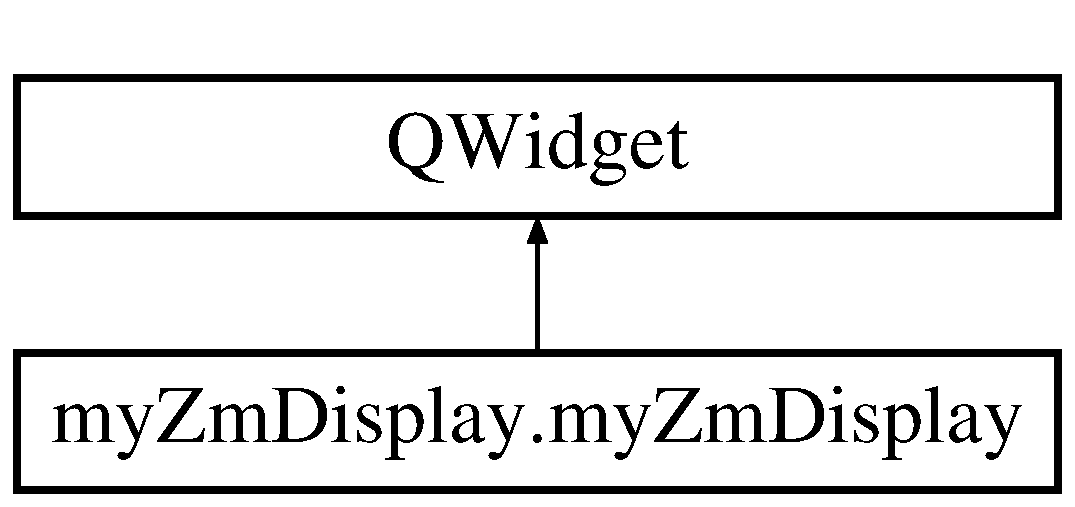
\includegraphics[height=2.000000cm]{classmy_zm_display_1_1my_zm_display}
\end{center}
\end{figure}
\subsection*{Public Member Functions}
\begin{DoxyCompactItemize}
\item 
def \hyperlink{classmy_zm_display_1_1my_zm_display_a54641fdc112a59527b6d8f449f7d37c7}{\-\_\-\-\_\-init\-\_\-\-\_\-}
\item 
def \hyperlink{classmy_zm_display_1_1my_zm_display_a217206bd5052930d7d07a909b65dcc0d}{set\-L\-U\-T}
\item 
def \hyperlink{classmy_zm_display_1_1my_zm_display_a97423d0a9d494ceaed4dae284d3d8450}{context\-Menu\-Kickoff}
\item 
def \hyperlink{classmy_zm_display_1_1my_zm_display_a2a6f289f9c749b30a41afddd9a9ccff2}{zoom\-On}
\item 
def \hyperlink{classmy_zm_display_1_1my_zm_display_ae19086d7b292cb945ef88264dcb239e8}{peak\-Add}
\item 
def \hyperlink{classmy_zm_display_1_1my_zm_display_abf543bfb38629b3ac50bb2077cab67cd}{set\-Peaks}
\item 
def \hyperlink{classmy_zm_display_1_1my_zm_display_acbc1fcd19eb140b6b08522900c66197b}{set\-Zm\-Fac}
\item 
def \hyperlink{classmy_zm_display_1_1my_zm_display_a424cb82d1b5af9f171d41b6aa8b4f933}{set\-Min\-Max}
\item 
def \hyperlink{classmy_zm_display_1_1my_zm_display_a236a9fc1081d57f3e8c528be5114d2ca}{set\-Fulldata}
\item 
def \hyperlink{classmy_zm_display_1_1my_zm_display_aa659a4760b6e6cb43c0d5ab6d68a505d}{write\-Q\-Image\-\_\-lut}
\item 
def \hyperlink{classmy_zm_display_1_1my_zm_display_a18fbc9063827c141d9c147ce9d9cafb5}{write\-Q\-Image\-\_\-update}
\item 
def \hyperlink{classmy_zm_display_1_1my_zm_display_a93f20083a078a129b63a75d7a05bfd3a}{mouse\-Press\-Event}
\item 
def \hyperlink{classmy_zm_display_1_1my_zm_display_a4abf307925064f63612b392ba2b5f0e3}{paint\-Event}
\item 
def \hyperlink{classmy_zm_display_1_1my_zm_display_a4a570d23a2199026dd99b659c7f1b15a}{apply\-Mask}
\end{DoxyCompactItemize}
\subsection*{Public Attributes}
\begin{DoxyCompactItemize}
\item 
\hyperlink{classmy_zm_display_1_1my_zm_display_ae957c679b9db235efff6747602ef60df}{peaks}
\item 
\hyperlink{classmy_zm_display_1_1my_zm_display_aaec1992079d9eaf789ed0e65cd55b99d}{zm\-Fac}
\item 
\hyperlink{classmy_zm_display_1_1my_zm_display_ab8eb21cf700300335ca6dedd71ccaba1}{disp\-Min}
\item 
\hyperlink{classmy_zm_display_1_1my_zm_display_ac03bdd7f4276b3d0aefe0dc7827143bc}{disp\-Max}
\item 
\hyperlink{classmy_zm_display_1_1my_zm_display_a108eff552f2c0e09db6c9d7ab2bdd401}{fulldata}
\item 
\hyperlink{classmy_zm_display_1_1my_zm_display_a97229acfaee29c678542d4c5f8cae694}{centloc}
\item 
\hyperlink{classmy_zm_display_1_1my_zm_display_a7aec333c091a737ace35d96d4a4e2991}{zoom\-Rect}
\item 
\hyperlink{classmy_zm_display_1_1my_zm_display_a27b868f986854ed524c451797f248028}{scale}
\item 
\hyperlink{classmy_zm_display_1_1my_zm_display_a54ce03f488e6c7852c76aca77a5c3895}{newx}
\item 
\hyperlink{classmy_zm_display_1_1my_zm_display_a736a1b9ec07a3565161b71961923da74}{newy}
\item 
\hyperlink{classmy_zm_display_1_1my_zm_display_ad535c3b024aab5d1cec5e6646e2bf60f}{qimage}
\item 
\hyperlink{classmy_zm_display_1_1my_zm_display_afd39f4afb5f5dc21acf35c5e6f050379}{load\-Image}
\item 
\hyperlink{classmy_zm_display_1_1my_zm_display_a10b4f37676eb840f0c9307365ea2dd48}{mymask}
\end{DoxyCompactItemize}
\subsection*{Static Public Attributes}
\begin{DoxyCompactItemize}
\item 
int \hyperlink{classmy_zm_display_1_1my_zm_display_a04859be3d64685448954dba22cdf78a4}{load\-Image} = 0
\item 
int \hyperlink{classmy_zm_display_1_1my_zm_display_a713e9fc2c8bf740fab1eb2e748b21f91}{disp\-Max} = 65535
\item 
int \hyperlink{classmy_zm_display_1_1my_zm_display_ab548c51111f007ef31a97994e8b410d8}{disp\-Min} = 0
\item 
int \hyperlink{classmy_zm_display_1_1my_zm_display_a70fe9d6a18cd3a6149fb5198448793c1}{zm\-Fac} = 4
\item 
int \hyperlink{classmy_zm_display_1_1my_zm_display_a88f396278207e78ff8c5e27dd6749b4c}{newx} = 0
\item 
int \hyperlink{classmy_zm_display_1_1my_zm_display_a0770201bb3e33e877d381cae65d6cfd9}{newy} = 0
\item 
\hyperlink{classmy_zm_display_1_1my_zm_display_a946f14d48450a167199b9ac2e14af7a4}{zoom\-Toggle} = True
\item 
\hyperlink{classmy_zm_display_1_1my_zm_display_a9b9dd02bf8545bd50e1d2f49a4be9ae3}{peak\-Toggle} = False
\item 
tuple \hyperlink{classmy_zm_display_1_1my_zm_display_a1caafb5ed9bfd30d1e992c754389a331}{zoom\-Rect} = Qt\-Core.\-Q\-Rect()
\item 
\hyperlink{classmy_zm_display_1_1my_zm_display_a5baf38a6e9c6609307240a3c4be0bca7}{apply\-Mask\-Flag} = False
\item 
tuple \hyperlink{classmy_zm_display_1_1my_zm_display_a7dbe912029d1343f3839c19050e235e3}{add\-Peak\-Signal} = Qt\-Core.\-pyqt\-Signal(Qt\-Core.\-Q\-Point)
\item 
tuple \hyperlink{classmy_zm_display_1_1my_zm_display_aa0ea7f897243bc2529551255f512d8c3}{set\-Button\-Mode\-Signal} = Qt\-Core.\-pyqt\-Signal(int)
\item 
tuple \hyperlink{classmy_zm_display_1_1my_zm_display_a24271d6d079df901d5128772fea0400b}{zm\-Rect\-Signal} = Qt\-Core.\-pyqt\-Signal(Qt\-Core.\-Q\-Rect)
\item 
tuple \hyperlink{classmy_zm_display_1_1my_zm_display_a47a941c14bc12031105afe99e85ef371}{imcoords\-Select\-Signal} = Qt\-Core.\-pyqt\-Signal(list)
\item 
tuple \hyperlink{classmy_zm_display_1_1my_zm_display_a6fd2b18cb86a3acb62e794079a9af2ca}{rgb\-\_\-lut} = np.\-zeros((3,256), dtype=np.\-uint8)
\end{DoxyCompactItemize}


\subsection{Constructor \& Destructor Documentation}
\hypertarget{classmy_zm_display_1_1my_zm_display_a54641fdc112a59527b6d8f449f7d37c7}{\index{my\-Zm\-Display\-::my\-Zm\-Display@{my\-Zm\-Display\-::my\-Zm\-Display}!\-\_\-\-\_\-init\-\_\-\-\_\-@{\-\_\-\-\_\-init\-\_\-\-\_\-}}
\index{\-\_\-\-\_\-init\-\_\-\-\_\-@{\-\_\-\-\_\-init\-\_\-\-\_\-}!myZmDisplay::myZmDisplay@{my\-Zm\-Display\-::my\-Zm\-Display}}
\subsubsection[{\-\_\-\-\_\-init\-\_\-\-\_\-}]{\setlength{\rightskip}{0pt plus 5cm}def my\-Zm\-Display.\-my\-Zm\-Display.\-\_\-\-\_\-init\-\_\-\-\_\- (
\begin{DoxyParamCaption}
\item[{}]{self, }
\item[{}]{parent}
\end{DoxyParamCaption}
)}}\label{classmy_zm_display_1_1my_zm_display_a54641fdc112a59527b6d8f449f7d37c7}


\subsection{Member Function Documentation}
\hypertarget{classmy_zm_display_1_1my_zm_display_a4a570d23a2199026dd99b659c7f1b15a}{\index{my\-Zm\-Display\-::my\-Zm\-Display@{my\-Zm\-Display\-::my\-Zm\-Display}!apply\-Mask@{apply\-Mask}}
\index{apply\-Mask@{apply\-Mask}!myZmDisplay::myZmDisplay@{my\-Zm\-Display\-::my\-Zm\-Display}}
\subsubsection[{apply\-Mask}]{\setlength{\rightskip}{0pt plus 5cm}def my\-Zm\-Display.\-my\-Zm\-Display.\-apply\-Mask (
\begin{DoxyParamCaption}
\item[{}]{self, }
\item[{}]{mask}
\end{DoxyParamCaption}
)}}\label{classmy_zm_display_1_1my_zm_display_a4a570d23a2199026dd99b659c7f1b15a}
\hypertarget{classmy_zm_display_1_1my_zm_display_a97423d0a9d494ceaed4dae284d3d8450}{\index{my\-Zm\-Display\-::my\-Zm\-Display@{my\-Zm\-Display\-::my\-Zm\-Display}!context\-Menu\-Kickoff@{context\-Menu\-Kickoff}}
\index{context\-Menu\-Kickoff@{context\-Menu\-Kickoff}!myZmDisplay::myZmDisplay@{my\-Zm\-Display\-::my\-Zm\-Display}}
\subsubsection[{context\-Menu\-Kickoff}]{\setlength{\rightskip}{0pt plus 5cm}def my\-Zm\-Display.\-my\-Zm\-Display.\-context\-Menu\-Kickoff (
\begin{DoxyParamCaption}
\item[{}]{self, }
\item[{}]{point}
\end{DoxyParamCaption}
)}}\label{classmy_zm_display_1_1my_zm_display_a97423d0a9d494ceaed4dae284d3d8450}
\hypertarget{classmy_zm_display_1_1my_zm_display_a93f20083a078a129b63a75d7a05bfd3a}{\index{my\-Zm\-Display\-::my\-Zm\-Display@{my\-Zm\-Display\-::my\-Zm\-Display}!mouse\-Press\-Event@{mouse\-Press\-Event}}
\index{mouse\-Press\-Event@{mouse\-Press\-Event}!myZmDisplay::myZmDisplay@{my\-Zm\-Display\-::my\-Zm\-Display}}
\subsubsection[{mouse\-Press\-Event}]{\setlength{\rightskip}{0pt plus 5cm}def my\-Zm\-Display.\-my\-Zm\-Display.\-mouse\-Press\-Event (
\begin{DoxyParamCaption}
\item[{}]{self, }
\item[{}]{event}
\end{DoxyParamCaption}
)}}\label{classmy_zm_display_1_1my_zm_display_a93f20083a078a129b63a75d7a05bfd3a}
\hypertarget{classmy_zm_display_1_1my_zm_display_a4abf307925064f63612b392ba2b5f0e3}{\index{my\-Zm\-Display\-::my\-Zm\-Display@{my\-Zm\-Display\-::my\-Zm\-Display}!paint\-Event@{paint\-Event}}
\index{paint\-Event@{paint\-Event}!myZmDisplay::myZmDisplay@{my\-Zm\-Display\-::my\-Zm\-Display}}
\subsubsection[{paint\-Event}]{\setlength{\rightskip}{0pt plus 5cm}def my\-Zm\-Display.\-my\-Zm\-Display.\-paint\-Event (
\begin{DoxyParamCaption}
\item[{}]{self, }
\item[{}]{event}
\end{DoxyParamCaption}
)}}\label{classmy_zm_display_1_1my_zm_display_a4abf307925064f63612b392ba2b5f0e3}
\hypertarget{classmy_zm_display_1_1my_zm_display_ae19086d7b292cb945ef88264dcb239e8}{\index{my\-Zm\-Display\-::my\-Zm\-Display@{my\-Zm\-Display\-::my\-Zm\-Display}!peak\-Add@{peak\-Add}}
\index{peak\-Add@{peak\-Add}!myZmDisplay::myZmDisplay@{my\-Zm\-Display\-::my\-Zm\-Display}}
\subsubsection[{peak\-Add}]{\setlength{\rightskip}{0pt plus 5cm}def my\-Zm\-Display.\-my\-Zm\-Display.\-peak\-Add (
\begin{DoxyParamCaption}
\item[{}]{self}
\end{DoxyParamCaption}
)}}\label{classmy_zm_display_1_1my_zm_display_ae19086d7b292cb945ef88264dcb239e8}
\hypertarget{classmy_zm_display_1_1my_zm_display_a236a9fc1081d57f3e8c528be5114d2ca}{\index{my\-Zm\-Display\-::my\-Zm\-Display@{my\-Zm\-Display\-::my\-Zm\-Display}!set\-Fulldata@{set\-Fulldata}}
\index{set\-Fulldata@{set\-Fulldata}!myZmDisplay::myZmDisplay@{my\-Zm\-Display\-::my\-Zm\-Display}}
\subsubsection[{set\-Fulldata}]{\setlength{\rightskip}{0pt plus 5cm}def my\-Zm\-Display.\-my\-Zm\-Display.\-set\-Fulldata (
\begin{DoxyParamCaption}
\item[{}]{self, }
\item[{}]{fd}
\end{DoxyParamCaption}
)}}\label{classmy_zm_display_1_1my_zm_display_a236a9fc1081d57f3e8c528be5114d2ca}
\hypertarget{classmy_zm_display_1_1my_zm_display_a217206bd5052930d7d07a909b65dcc0d}{\index{my\-Zm\-Display\-::my\-Zm\-Display@{my\-Zm\-Display\-::my\-Zm\-Display}!set\-L\-U\-T@{set\-L\-U\-T}}
\index{set\-L\-U\-T@{set\-L\-U\-T}!myZmDisplay::myZmDisplay@{my\-Zm\-Display\-::my\-Zm\-Display}}
\subsubsection[{set\-L\-U\-T}]{\setlength{\rightskip}{0pt plus 5cm}def my\-Zm\-Display.\-my\-Zm\-Display.\-set\-L\-U\-T (
\begin{DoxyParamCaption}
\item[{}]{self, }
\item[{}]{arr}
\end{DoxyParamCaption}
)}}\label{classmy_zm_display_1_1my_zm_display_a217206bd5052930d7d07a909b65dcc0d}
\hypertarget{classmy_zm_display_1_1my_zm_display_a424cb82d1b5af9f171d41b6aa8b4f933}{\index{my\-Zm\-Display\-::my\-Zm\-Display@{my\-Zm\-Display\-::my\-Zm\-Display}!set\-Min\-Max@{set\-Min\-Max}}
\index{set\-Min\-Max@{set\-Min\-Max}!myZmDisplay::myZmDisplay@{my\-Zm\-Display\-::my\-Zm\-Display}}
\subsubsection[{set\-Min\-Max}]{\setlength{\rightskip}{0pt plus 5cm}def my\-Zm\-Display.\-my\-Zm\-Display.\-set\-Min\-Max (
\begin{DoxyParamCaption}
\item[{}]{self, }
\item[{}]{min, }
\item[{}]{max}
\end{DoxyParamCaption}
)}}\label{classmy_zm_display_1_1my_zm_display_a424cb82d1b5af9f171d41b6aa8b4f933}
\hypertarget{classmy_zm_display_1_1my_zm_display_abf543bfb38629b3ac50bb2077cab67cd}{\index{my\-Zm\-Display\-::my\-Zm\-Display@{my\-Zm\-Display\-::my\-Zm\-Display}!set\-Peaks@{set\-Peaks}}
\index{set\-Peaks@{set\-Peaks}!myZmDisplay::myZmDisplay@{my\-Zm\-Display\-::my\-Zm\-Display}}
\subsubsection[{set\-Peaks}]{\setlength{\rightskip}{0pt plus 5cm}def my\-Zm\-Display.\-my\-Zm\-Display.\-set\-Peaks (
\begin{DoxyParamCaption}
\item[{}]{self, }
\item[{}]{pks}
\end{DoxyParamCaption}
)}}\label{classmy_zm_display_1_1my_zm_display_abf543bfb38629b3ac50bb2077cab67cd}
\hypertarget{classmy_zm_display_1_1my_zm_display_acbc1fcd19eb140b6b08522900c66197b}{\index{my\-Zm\-Display\-::my\-Zm\-Display@{my\-Zm\-Display\-::my\-Zm\-Display}!set\-Zm\-Fac@{set\-Zm\-Fac}}
\index{set\-Zm\-Fac@{set\-Zm\-Fac}!myZmDisplay::myZmDisplay@{my\-Zm\-Display\-::my\-Zm\-Display}}
\subsubsection[{set\-Zm\-Fac}]{\setlength{\rightskip}{0pt plus 5cm}def my\-Zm\-Display.\-my\-Zm\-Display.\-set\-Zm\-Fac (
\begin{DoxyParamCaption}
\item[{}]{self, }
\item[{}]{zm}
\end{DoxyParamCaption}
)}}\label{classmy_zm_display_1_1my_zm_display_acbc1fcd19eb140b6b08522900c66197b}
\hypertarget{classmy_zm_display_1_1my_zm_display_aa659a4760b6e6cb43c0d5ab6d68a505d}{\index{my\-Zm\-Display\-::my\-Zm\-Display@{my\-Zm\-Display\-::my\-Zm\-Display}!write\-Q\-Image\-\_\-lut@{write\-Q\-Image\-\_\-lut}}
\index{write\-Q\-Image\-\_\-lut@{write\-Q\-Image\-\_\-lut}!myZmDisplay::myZmDisplay@{my\-Zm\-Display\-::my\-Zm\-Display}}
\subsubsection[{write\-Q\-Image\-\_\-lut}]{\setlength{\rightskip}{0pt plus 5cm}def my\-Zm\-Display.\-my\-Zm\-Display.\-write\-Q\-Image\-\_\-lut (
\begin{DoxyParamCaption}
\item[{}]{self, }
\item[{}]{fulldata, }
\item[{}]{centloc}
\end{DoxyParamCaption}
)}}\label{classmy_zm_display_1_1my_zm_display_aa659a4760b6e6cb43c0d5ab6d68a505d}
\hypertarget{classmy_zm_display_1_1my_zm_display_a18fbc9063827c141d9c147ce9d9cafb5}{\index{my\-Zm\-Display\-::my\-Zm\-Display@{my\-Zm\-Display\-::my\-Zm\-Display}!write\-Q\-Image\-\_\-update@{write\-Q\-Image\-\_\-update}}
\index{write\-Q\-Image\-\_\-update@{write\-Q\-Image\-\_\-update}!myZmDisplay::myZmDisplay@{my\-Zm\-Display\-::my\-Zm\-Display}}
\subsubsection[{write\-Q\-Image\-\_\-update}]{\setlength{\rightskip}{0pt plus 5cm}def my\-Zm\-Display.\-my\-Zm\-Display.\-write\-Q\-Image\-\_\-update (
\begin{DoxyParamCaption}
\item[{}]{self}
\end{DoxyParamCaption}
)}}\label{classmy_zm_display_1_1my_zm_display_a18fbc9063827c141d9c147ce9d9cafb5}
\hypertarget{classmy_zm_display_1_1my_zm_display_a2a6f289f9c749b30a41afddd9a9ccff2}{\index{my\-Zm\-Display\-::my\-Zm\-Display@{my\-Zm\-Display\-::my\-Zm\-Display}!zoom\-On@{zoom\-On}}
\index{zoom\-On@{zoom\-On}!myZmDisplay::myZmDisplay@{my\-Zm\-Display\-::my\-Zm\-Display}}
\subsubsection[{zoom\-On}]{\setlength{\rightskip}{0pt plus 5cm}def my\-Zm\-Display.\-my\-Zm\-Display.\-zoom\-On (
\begin{DoxyParamCaption}
\item[{}]{self}
\end{DoxyParamCaption}
)}}\label{classmy_zm_display_1_1my_zm_display_a2a6f289f9c749b30a41afddd9a9ccff2}


\subsection{Member Data Documentation}
\hypertarget{classmy_zm_display_1_1my_zm_display_a7dbe912029d1343f3839c19050e235e3}{\index{my\-Zm\-Display\-::my\-Zm\-Display@{my\-Zm\-Display\-::my\-Zm\-Display}!add\-Peak\-Signal@{add\-Peak\-Signal}}
\index{add\-Peak\-Signal@{add\-Peak\-Signal}!myZmDisplay::myZmDisplay@{my\-Zm\-Display\-::my\-Zm\-Display}}
\subsubsection[{add\-Peak\-Signal}]{\setlength{\rightskip}{0pt plus 5cm}tuple my\-Zm\-Display.\-my\-Zm\-Display.\-add\-Peak\-Signal = Qt\-Core.\-pyqt\-Signal(Qt\-Core.\-Q\-Point)\hspace{0.3cm}{\ttfamily [static]}}}\label{classmy_zm_display_1_1my_zm_display_a7dbe912029d1343f3839c19050e235e3}
\hypertarget{classmy_zm_display_1_1my_zm_display_a5baf38a6e9c6609307240a3c4be0bca7}{\index{my\-Zm\-Display\-::my\-Zm\-Display@{my\-Zm\-Display\-::my\-Zm\-Display}!apply\-Mask\-Flag@{apply\-Mask\-Flag}}
\index{apply\-Mask\-Flag@{apply\-Mask\-Flag}!myZmDisplay::myZmDisplay@{my\-Zm\-Display\-::my\-Zm\-Display}}
\subsubsection[{apply\-Mask\-Flag}]{\setlength{\rightskip}{0pt plus 5cm}my\-Zm\-Display.\-my\-Zm\-Display.\-apply\-Mask\-Flag = False\hspace{0.3cm}{\ttfamily [static]}}}\label{classmy_zm_display_1_1my_zm_display_a5baf38a6e9c6609307240a3c4be0bca7}
\hypertarget{classmy_zm_display_1_1my_zm_display_a97229acfaee29c678542d4c5f8cae694}{\index{my\-Zm\-Display\-::my\-Zm\-Display@{my\-Zm\-Display\-::my\-Zm\-Display}!centloc@{centloc}}
\index{centloc@{centloc}!myZmDisplay::myZmDisplay@{my\-Zm\-Display\-::my\-Zm\-Display}}
\subsubsection[{centloc}]{\setlength{\rightskip}{0pt plus 5cm}my\-Zm\-Display.\-my\-Zm\-Display.\-centloc}}\label{classmy_zm_display_1_1my_zm_display_a97229acfaee29c678542d4c5f8cae694}
\hypertarget{classmy_zm_display_1_1my_zm_display_a713e9fc2c8bf740fab1eb2e748b21f91}{\index{my\-Zm\-Display\-::my\-Zm\-Display@{my\-Zm\-Display\-::my\-Zm\-Display}!disp\-Max@{disp\-Max}}
\index{disp\-Max@{disp\-Max}!myZmDisplay::myZmDisplay@{my\-Zm\-Display\-::my\-Zm\-Display}}
\subsubsection[{disp\-Max}]{\setlength{\rightskip}{0pt plus 5cm}int my\-Zm\-Display.\-my\-Zm\-Display.\-disp\-Max = 65535\hspace{0.3cm}{\ttfamily [static]}}}\label{classmy_zm_display_1_1my_zm_display_a713e9fc2c8bf740fab1eb2e748b21f91}
\hypertarget{classmy_zm_display_1_1my_zm_display_ac03bdd7f4276b3d0aefe0dc7827143bc}{\index{my\-Zm\-Display\-::my\-Zm\-Display@{my\-Zm\-Display\-::my\-Zm\-Display}!disp\-Max@{disp\-Max}}
\index{disp\-Max@{disp\-Max}!myZmDisplay::myZmDisplay@{my\-Zm\-Display\-::my\-Zm\-Display}}
\subsubsection[{disp\-Max}]{\setlength{\rightskip}{0pt plus 5cm}my\-Zm\-Display.\-my\-Zm\-Display.\-disp\-Max}}\label{classmy_zm_display_1_1my_zm_display_ac03bdd7f4276b3d0aefe0dc7827143bc}
\hypertarget{classmy_zm_display_1_1my_zm_display_ab548c51111f007ef31a97994e8b410d8}{\index{my\-Zm\-Display\-::my\-Zm\-Display@{my\-Zm\-Display\-::my\-Zm\-Display}!disp\-Min@{disp\-Min}}
\index{disp\-Min@{disp\-Min}!myZmDisplay::myZmDisplay@{my\-Zm\-Display\-::my\-Zm\-Display}}
\subsubsection[{disp\-Min}]{\setlength{\rightskip}{0pt plus 5cm}int my\-Zm\-Display.\-my\-Zm\-Display.\-disp\-Min = 0\hspace{0.3cm}{\ttfamily [static]}}}\label{classmy_zm_display_1_1my_zm_display_ab548c51111f007ef31a97994e8b410d8}
\hypertarget{classmy_zm_display_1_1my_zm_display_ab8eb21cf700300335ca6dedd71ccaba1}{\index{my\-Zm\-Display\-::my\-Zm\-Display@{my\-Zm\-Display\-::my\-Zm\-Display}!disp\-Min@{disp\-Min}}
\index{disp\-Min@{disp\-Min}!myZmDisplay::myZmDisplay@{my\-Zm\-Display\-::my\-Zm\-Display}}
\subsubsection[{disp\-Min}]{\setlength{\rightskip}{0pt plus 5cm}my\-Zm\-Display.\-my\-Zm\-Display.\-disp\-Min}}\label{classmy_zm_display_1_1my_zm_display_ab8eb21cf700300335ca6dedd71ccaba1}
\hypertarget{classmy_zm_display_1_1my_zm_display_a108eff552f2c0e09db6c9d7ab2bdd401}{\index{my\-Zm\-Display\-::my\-Zm\-Display@{my\-Zm\-Display\-::my\-Zm\-Display}!fulldata@{fulldata}}
\index{fulldata@{fulldata}!myZmDisplay::myZmDisplay@{my\-Zm\-Display\-::my\-Zm\-Display}}
\subsubsection[{fulldata}]{\setlength{\rightskip}{0pt plus 5cm}my\-Zm\-Display.\-my\-Zm\-Display.\-fulldata}}\label{classmy_zm_display_1_1my_zm_display_a108eff552f2c0e09db6c9d7ab2bdd401}
\hypertarget{classmy_zm_display_1_1my_zm_display_a47a941c14bc12031105afe99e85ef371}{\index{my\-Zm\-Display\-::my\-Zm\-Display@{my\-Zm\-Display\-::my\-Zm\-Display}!imcoords\-Select\-Signal@{imcoords\-Select\-Signal}}
\index{imcoords\-Select\-Signal@{imcoords\-Select\-Signal}!myZmDisplay::myZmDisplay@{my\-Zm\-Display\-::my\-Zm\-Display}}
\subsubsection[{imcoords\-Select\-Signal}]{\setlength{\rightskip}{0pt plus 5cm}tuple my\-Zm\-Display.\-my\-Zm\-Display.\-imcoords\-Select\-Signal = Qt\-Core.\-pyqt\-Signal(list)\hspace{0.3cm}{\ttfamily [static]}}}\label{classmy_zm_display_1_1my_zm_display_a47a941c14bc12031105afe99e85ef371}
\hypertarget{classmy_zm_display_1_1my_zm_display_a04859be3d64685448954dba22cdf78a4}{\index{my\-Zm\-Display\-::my\-Zm\-Display@{my\-Zm\-Display\-::my\-Zm\-Display}!load\-Image@{load\-Image}}
\index{load\-Image@{load\-Image}!myZmDisplay::myZmDisplay@{my\-Zm\-Display\-::my\-Zm\-Display}}
\subsubsection[{load\-Image}]{\setlength{\rightskip}{0pt plus 5cm}int my\-Zm\-Display.\-my\-Zm\-Display.\-load\-Image = 0\hspace{0.3cm}{\ttfamily [static]}}}\label{classmy_zm_display_1_1my_zm_display_a04859be3d64685448954dba22cdf78a4}
\hypertarget{classmy_zm_display_1_1my_zm_display_afd39f4afb5f5dc21acf35c5e6f050379}{\index{my\-Zm\-Display\-::my\-Zm\-Display@{my\-Zm\-Display\-::my\-Zm\-Display}!load\-Image@{load\-Image}}
\index{load\-Image@{load\-Image}!myZmDisplay::myZmDisplay@{my\-Zm\-Display\-::my\-Zm\-Display}}
\subsubsection[{load\-Image}]{\setlength{\rightskip}{0pt plus 5cm}my\-Zm\-Display.\-my\-Zm\-Display.\-load\-Image}}\label{classmy_zm_display_1_1my_zm_display_afd39f4afb5f5dc21acf35c5e6f050379}
\hypertarget{classmy_zm_display_1_1my_zm_display_a10b4f37676eb840f0c9307365ea2dd48}{\index{my\-Zm\-Display\-::my\-Zm\-Display@{my\-Zm\-Display\-::my\-Zm\-Display}!mymask@{mymask}}
\index{mymask@{mymask}!myZmDisplay::myZmDisplay@{my\-Zm\-Display\-::my\-Zm\-Display}}
\subsubsection[{mymask}]{\setlength{\rightskip}{0pt plus 5cm}my\-Zm\-Display.\-my\-Zm\-Display.\-mymask}}\label{classmy_zm_display_1_1my_zm_display_a10b4f37676eb840f0c9307365ea2dd48}
\hypertarget{classmy_zm_display_1_1my_zm_display_a88f396278207e78ff8c5e27dd6749b4c}{\index{my\-Zm\-Display\-::my\-Zm\-Display@{my\-Zm\-Display\-::my\-Zm\-Display}!newx@{newx}}
\index{newx@{newx}!myZmDisplay::myZmDisplay@{my\-Zm\-Display\-::my\-Zm\-Display}}
\subsubsection[{newx}]{\setlength{\rightskip}{0pt plus 5cm}int my\-Zm\-Display.\-my\-Zm\-Display.\-newx = 0\hspace{0.3cm}{\ttfamily [static]}}}\label{classmy_zm_display_1_1my_zm_display_a88f396278207e78ff8c5e27dd6749b4c}
\hypertarget{classmy_zm_display_1_1my_zm_display_a54ce03f488e6c7852c76aca77a5c3895}{\index{my\-Zm\-Display\-::my\-Zm\-Display@{my\-Zm\-Display\-::my\-Zm\-Display}!newx@{newx}}
\index{newx@{newx}!myZmDisplay::myZmDisplay@{my\-Zm\-Display\-::my\-Zm\-Display}}
\subsubsection[{newx}]{\setlength{\rightskip}{0pt plus 5cm}my\-Zm\-Display.\-my\-Zm\-Display.\-newx}}\label{classmy_zm_display_1_1my_zm_display_a54ce03f488e6c7852c76aca77a5c3895}
\hypertarget{classmy_zm_display_1_1my_zm_display_a0770201bb3e33e877d381cae65d6cfd9}{\index{my\-Zm\-Display\-::my\-Zm\-Display@{my\-Zm\-Display\-::my\-Zm\-Display}!newy@{newy}}
\index{newy@{newy}!myZmDisplay::myZmDisplay@{my\-Zm\-Display\-::my\-Zm\-Display}}
\subsubsection[{newy}]{\setlength{\rightskip}{0pt plus 5cm}int my\-Zm\-Display.\-my\-Zm\-Display.\-newy = 0\hspace{0.3cm}{\ttfamily [static]}}}\label{classmy_zm_display_1_1my_zm_display_a0770201bb3e33e877d381cae65d6cfd9}
\hypertarget{classmy_zm_display_1_1my_zm_display_a736a1b9ec07a3565161b71961923da74}{\index{my\-Zm\-Display\-::my\-Zm\-Display@{my\-Zm\-Display\-::my\-Zm\-Display}!newy@{newy}}
\index{newy@{newy}!myZmDisplay::myZmDisplay@{my\-Zm\-Display\-::my\-Zm\-Display}}
\subsubsection[{newy}]{\setlength{\rightskip}{0pt plus 5cm}my\-Zm\-Display.\-my\-Zm\-Display.\-newy}}\label{classmy_zm_display_1_1my_zm_display_a736a1b9ec07a3565161b71961923da74}
\hypertarget{classmy_zm_display_1_1my_zm_display_ae957c679b9db235efff6747602ef60df}{\index{my\-Zm\-Display\-::my\-Zm\-Display@{my\-Zm\-Display\-::my\-Zm\-Display}!peaks@{peaks}}
\index{peaks@{peaks}!myZmDisplay::myZmDisplay@{my\-Zm\-Display\-::my\-Zm\-Display}}
\subsubsection[{peaks}]{\setlength{\rightskip}{0pt plus 5cm}my\-Zm\-Display.\-my\-Zm\-Display.\-peaks}}\label{classmy_zm_display_1_1my_zm_display_ae957c679b9db235efff6747602ef60df}
\hypertarget{classmy_zm_display_1_1my_zm_display_a9b9dd02bf8545bd50e1d2f49a4be9ae3}{\index{my\-Zm\-Display\-::my\-Zm\-Display@{my\-Zm\-Display\-::my\-Zm\-Display}!peak\-Toggle@{peak\-Toggle}}
\index{peak\-Toggle@{peak\-Toggle}!myZmDisplay::myZmDisplay@{my\-Zm\-Display\-::my\-Zm\-Display}}
\subsubsection[{peak\-Toggle}]{\setlength{\rightskip}{0pt plus 5cm}my\-Zm\-Display.\-my\-Zm\-Display.\-peak\-Toggle = False\hspace{0.3cm}{\ttfamily [static]}}}\label{classmy_zm_display_1_1my_zm_display_a9b9dd02bf8545bd50e1d2f49a4be9ae3}
\hypertarget{classmy_zm_display_1_1my_zm_display_ad535c3b024aab5d1cec5e6646e2bf60f}{\index{my\-Zm\-Display\-::my\-Zm\-Display@{my\-Zm\-Display\-::my\-Zm\-Display}!qimage@{qimage}}
\index{qimage@{qimage}!myZmDisplay::myZmDisplay@{my\-Zm\-Display\-::my\-Zm\-Display}}
\subsubsection[{qimage}]{\setlength{\rightskip}{0pt plus 5cm}my\-Zm\-Display.\-my\-Zm\-Display.\-qimage}}\label{classmy_zm_display_1_1my_zm_display_ad535c3b024aab5d1cec5e6646e2bf60f}
\hypertarget{classmy_zm_display_1_1my_zm_display_a6fd2b18cb86a3acb62e794079a9af2ca}{\index{my\-Zm\-Display\-::my\-Zm\-Display@{my\-Zm\-Display\-::my\-Zm\-Display}!rgb\-\_\-lut@{rgb\-\_\-lut}}
\index{rgb\-\_\-lut@{rgb\-\_\-lut}!myZmDisplay::myZmDisplay@{my\-Zm\-Display\-::my\-Zm\-Display}}
\subsubsection[{rgb\-\_\-lut}]{\setlength{\rightskip}{0pt plus 5cm}tuple my\-Zm\-Display.\-my\-Zm\-Display.\-rgb\-\_\-lut = np.\-zeros((3,256), dtype=np.\-uint8)\hspace{0.3cm}{\ttfamily [static]}}}\label{classmy_zm_display_1_1my_zm_display_a6fd2b18cb86a3acb62e794079a9af2ca}
\hypertarget{classmy_zm_display_1_1my_zm_display_a27b868f986854ed524c451797f248028}{\index{my\-Zm\-Display\-::my\-Zm\-Display@{my\-Zm\-Display\-::my\-Zm\-Display}!scale@{scale}}
\index{scale@{scale}!myZmDisplay::myZmDisplay@{my\-Zm\-Display\-::my\-Zm\-Display}}
\subsubsection[{scale}]{\setlength{\rightskip}{0pt plus 5cm}my\-Zm\-Display.\-my\-Zm\-Display.\-scale}}\label{classmy_zm_display_1_1my_zm_display_a27b868f986854ed524c451797f248028}
\hypertarget{classmy_zm_display_1_1my_zm_display_aa0ea7f897243bc2529551255f512d8c3}{\index{my\-Zm\-Display\-::my\-Zm\-Display@{my\-Zm\-Display\-::my\-Zm\-Display}!set\-Button\-Mode\-Signal@{set\-Button\-Mode\-Signal}}
\index{set\-Button\-Mode\-Signal@{set\-Button\-Mode\-Signal}!myZmDisplay::myZmDisplay@{my\-Zm\-Display\-::my\-Zm\-Display}}
\subsubsection[{set\-Button\-Mode\-Signal}]{\setlength{\rightskip}{0pt plus 5cm}tuple my\-Zm\-Display.\-my\-Zm\-Display.\-set\-Button\-Mode\-Signal = Qt\-Core.\-pyqt\-Signal(int)\hspace{0.3cm}{\ttfamily [static]}}}\label{classmy_zm_display_1_1my_zm_display_aa0ea7f897243bc2529551255f512d8c3}
\hypertarget{classmy_zm_display_1_1my_zm_display_a70fe9d6a18cd3a6149fb5198448793c1}{\index{my\-Zm\-Display\-::my\-Zm\-Display@{my\-Zm\-Display\-::my\-Zm\-Display}!zm\-Fac@{zm\-Fac}}
\index{zm\-Fac@{zm\-Fac}!myZmDisplay::myZmDisplay@{my\-Zm\-Display\-::my\-Zm\-Display}}
\subsubsection[{zm\-Fac}]{\setlength{\rightskip}{0pt plus 5cm}int my\-Zm\-Display.\-my\-Zm\-Display.\-zm\-Fac = 4\hspace{0.3cm}{\ttfamily [static]}}}\label{classmy_zm_display_1_1my_zm_display_a70fe9d6a18cd3a6149fb5198448793c1}
\hypertarget{classmy_zm_display_1_1my_zm_display_aaec1992079d9eaf789ed0e65cd55b99d}{\index{my\-Zm\-Display\-::my\-Zm\-Display@{my\-Zm\-Display\-::my\-Zm\-Display}!zm\-Fac@{zm\-Fac}}
\index{zm\-Fac@{zm\-Fac}!myZmDisplay::myZmDisplay@{my\-Zm\-Display\-::my\-Zm\-Display}}
\subsubsection[{zm\-Fac}]{\setlength{\rightskip}{0pt plus 5cm}my\-Zm\-Display.\-my\-Zm\-Display.\-zm\-Fac}}\label{classmy_zm_display_1_1my_zm_display_aaec1992079d9eaf789ed0e65cd55b99d}
\hypertarget{classmy_zm_display_1_1my_zm_display_a24271d6d079df901d5128772fea0400b}{\index{my\-Zm\-Display\-::my\-Zm\-Display@{my\-Zm\-Display\-::my\-Zm\-Display}!zm\-Rect\-Signal@{zm\-Rect\-Signal}}
\index{zm\-Rect\-Signal@{zm\-Rect\-Signal}!myZmDisplay::myZmDisplay@{my\-Zm\-Display\-::my\-Zm\-Display}}
\subsubsection[{zm\-Rect\-Signal}]{\setlength{\rightskip}{0pt plus 5cm}tuple my\-Zm\-Display.\-my\-Zm\-Display.\-zm\-Rect\-Signal = Qt\-Core.\-pyqt\-Signal(Qt\-Core.\-Q\-Rect)\hspace{0.3cm}{\ttfamily [static]}}}\label{classmy_zm_display_1_1my_zm_display_a24271d6d079df901d5128772fea0400b}
\hypertarget{classmy_zm_display_1_1my_zm_display_a1caafb5ed9bfd30d1e992c754389a331}{\index{my\-Zm\-Display\-::my\-Zm\-Display@{my\-Zm\-Display\-::my\-Zm\-Display}!zoom\-Rect@{zoom\-Rect}}
\index{zoom\-Rect@{zoom\-Rect}!myZmDisplay::myZmDisplay@{my\-Zm\-Display\-::my\-Zm\-Display}}
\subsubsection[{zoom\-Rect}]{\setlength{\rightskip}{0pt plus 5cm}tuple my\-Zm\-Display.\-my\-Zm\-Display.\-zoom\-Rect = Qt\-Core.\-Q\-Rect()\hspace{0.3cm}{\ttfamily [static]}}}\label{classmy_zm_display_1_1my_zm_display_a1caafb5ed9bfd30d1e992c754389a331}
\hypertarget{classmy_zm_display_1_1my_zm_display_a7aec333c091a737ace35d96d4a4e2991}{\index{my\-Zm\-Display\-::my\-Zm\-Display@{my\-Zm\-Display\-::my\-Zm\-Display}!zoom\-Rect@{zoom\-Rect}}
\index{zoom\-Rect@{zoom\-Rect}!myZmDisplay::myZmDisplay@{my\-Zm\-Display\-::my\-Zm\-Display}}
\subsubsection[{zoom\-Rect}]{\setlength{\rightskip}{0pt plus 5cm}my\-Zm\-Display.\-my\-Zm\-Display.\-zoom\-Rect}}\label{classmy_zm_display_1_1my_zm_display_a7aec333c091a737ace35d96d4a4e2991}
\hypertarget{classmy_zm_display_1_1my_zm_display_a946f14d48450a167199b9ac2e14af7a4}{\index{my\-Zm\-Display\-::my\-Zm\-Display@{my\-Zm\-Display\-::my\-Zm\-Display}!zoom\-Toggle@{zoom\-Toggle}}
\index{zoom\-Toggle@{zoom\-Toggle}!myZmDisplay::myZmDisplay@{my\-Zm\-Display\-::my\-Zm\-Display}}
\subsubsection[{zoom\-Toggle}]{\setlength{\rightskip}{0pt plus 5cm}my\-Zm\-Display.\-my\-Zm\-Display.\-zoom\-Toggle = True\hspace{0.3cm}{\ttfamily [static]}}}\label{classmy_zm_display_1_1my_zm_display_a946f14d48450a167199b9ac2e14af7a4}


The documentation for this class was generated from the following file\-:\begin{DoxyCompactItemize}
\item 
workdir/atrex/\-Software/\hyperlink{my_zm_display_8py}{my\-Zm\-Display.\-py}\end{DoxyCompactItemize}

\hypertarget{classmy_zm_peak_display_1_1my_zm_peak_display}{\section{my\-Zm\-Peak\-Display.\-my\-Zm\-Peak\-Display Class Reference}
\label{classmy_zm_peak_display_1_1my_zm_peak_display}\index{my\-Zm\-Peak\-Display.\-my\-Zm\-Peak\-Display@{my\-Zm\-Peak\-Display.\-my\-Zm\-Peak\-Display}}
}
Inheritance diagram for my\-Zm\-Peak\-Display.\-my\-Zm\-Peak\-Display\-:\begin{figure}[H]
\begin{center}
\leavevmode
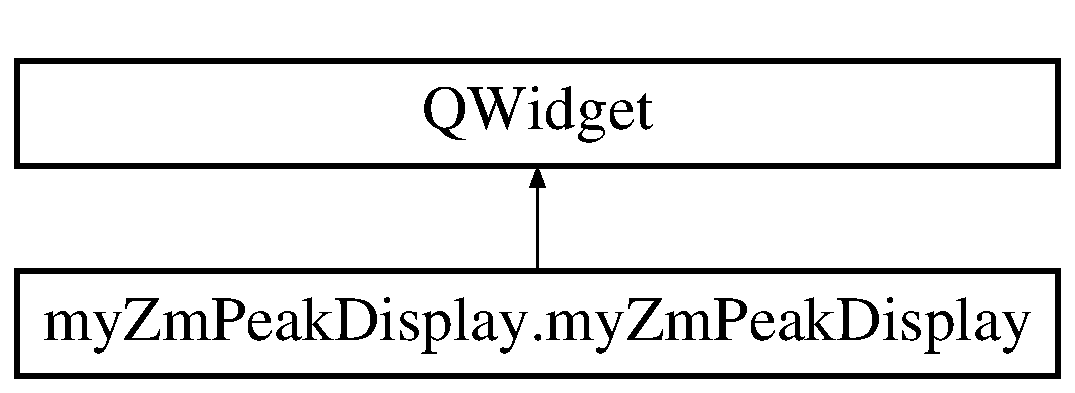
\includegraphics[height=2.000000cm]{classmy_zm_peak_display_1_1my_zm_peak_display}
\end{center}
\end{figure}
\subsection*{Public Member Functions}
\begin{DoxyCompactItemize}
\item 
def \hyperlink{classmy_zm_peak_display_1_1my_zm_peak_display_a348a15b190a012ffee26f7526d2eca3c}{\-\_\-\-\_\-init\-\_\-\-\_\-}
\item 
def \hyperlink{classmy_zm_peak_display_1_1my_zm_peak_display_aab9ac5a869bd132456f71fe022b2ad65}{calc\-Histo}
\item 
def \hyperlink{classmy_zm_peak_display_1_1my_zm_peak_display_a3a7fbef40f5613213deb5367a19f7857}{set\-Min\-Max}
\item 
def \hyperlink{classmy_zm_peak_display_1_1my_zm_peak_display_af002add8e8eb6c55820cc2e12a8457c9}{array\-To\-Q\-Image}
\item 
def \hyperlink{classmy_zm_peak_display_1_1my_zm_peak_display_ae50e3adcca21aee551f8d757d77b9eba}{write\-Q\-Image\-\_\-lut}
\item 
def \hyperlink{classmy_zm_peak_display_1_1my_zm_peak_display_abd1762a6b6ac58060a7a3d5f2fc4ff1a}{mouse\-Press\-Event}
\item 
def \hyperlink{classmy_zm_peak_display_1_1my_zm_peak_display_a7bce038050bb5bdd6b3d58be7ef13f00}{mouse\-Release\-Event}
\item 
def \hyperlink{classmy_zm_peak_display_1_1my_zm_peak_display_a86086ce776ea26bbb7c84dd6f49a3064}{set\-Bar\-Flag}
\item 
def \hyperlink{classmy_zm_peak_display_1_1my_zm_peak_display_ada885fc1335a833a72ce8f65078c1fab}{mouse\-Move\-Event}
\item 
def \hyperlink{classmy_zm_peak_display_1_1my_zm_peak_display_a86086ce776ea26bbb7c84dd6f49a3064}{set\-Bar\-Flag}
\item 
def \hyperlink{classmy_zm_peak_display_1_1my_zm_peak_display_a45a5009c5ecc96d9a6ff350600478b37}{paint\-Event}
\end{DoxyCompactItemize}
\subsection*{Public Attributes}
\begin{DoxyCompactItemize}
\item 
\hyperlink{classmy_zm_peak_display_1_1my_zm_peak_display_a2a58f32f3a30578f0d511a206dac4d92}{ind\-\_\-5}
\item 
\hyperlink{classmy_zm_peak_display_1_1my_zm_peak_display_a188042c43b850fa601b05ef9b45983b7}{ind\-\_\-95}
\item 
\hyperlink{classmy_zm_peak_display_1_1my_zm_peak_display_adc972d94702bf72b1aa7f9bafa51a523}{disp\-Max}
\item 
\hyperlink{classmy_zm_peak_display_1_1my_zm_peak_display_a82777e7574c238178144464a0a4c9dd5}{disp\-Min}
\item 
\hyperlink{classmy_zm_peak_display_1_1my_zm_peak_display_a4d79fa930b80664bf9c661c69c90e45a}{scale}
\item 
\hyperlink{classmy_zm_peak_display_1_1my_zm_peak_display_ac30db7d7e88a260a660c73842cc7e70c}{newx}
\item 
\hyperlink{classmy_zm_peak_display_1_1my_zm_peak_display_aa5d3657333093135e384f3bfa49a9ddf}{newy}
\item 
\hyperlink{classmy_zm_peak_display_1_1my_zm_peak_display_a1ff0a93d46b719217c98326afd23efc0}{qimage}
\item 
\hyperlink{classmy_zm_peak_display_1_1my_zm_peak_display_a90d2173fc5c4bda615e1f6e2cda08d89}{load\-Image}
\item 
\hyperlink{classmy_zm_peak_display_1_1my_zm_peak_display_a72f7fc0519471f766cacc379811b3de0}{startx}
\item 
\hyperlink{classmy_zm_peak_display_1_1my_zm_peak_display_a18be92130080c324da24bfd8bb70d1f0}{starty}
\item 
\hyperlink{classmy_zm_peak_display_1_1my_zm_peak_display_ad5645653988974bebc739532eac8ef86}{ns}
\item 
\hyperlink{classmy_zm_peak_display_1_1my_zm_peak_display_aa08f61c355a9ebaf1ee628a10ba72a02}{nl}
\item 
\hyperlink{classmy_zm_peak_display_1_1my_zm_peak_display_a3418f94ca8d8f74f38e83a9857cacd5b}{zm\-Fac}
\item 
\hyperlink{classmy_zm_peak_display_1_1my_zm_peak_display_ae1ca848339601ec3d5cdd9409a683ce9}{vbarloc}
\item 
\hyperlink{classmy_zm_peak_display_1_1my_zm_peak_display_ad44f714b1fc1fc724d16ebdb4d910574}{hbarloc}
\item 
\hyperlink{classmy_zm_peak_display_1_1my_zm_peak_display_adf7a9d7f5ca82215805acbc121e9d42d}{vbarloc\-\_\-orig}
\item 
\hyperlink{classmy_zm_peak_display_1_1my_zm_peak_display_a9f46ba18c0baa95bd2c7ec8b70dcddbe}{hbarloc\-\_\-orig}
\item 
\hyperlink{classmy_zm_peak_display_1_1my_zm_peak_display_a2ad52ce54407b62ce8829e538a845049}{fulldata}
\item 
\hyperlink{classmy_zm_peak_display_1_1my_zm_peak_display_aead8ab13c78f41a35434760be199264a}{zoom\-Rect}
\item 
\hyperlink{classmy_zm_peak_display_1_1my_zm_peak_display_ab0a84e7b6930d7b42d51c4bc0a2fc4ec}{bar\-Flag}
\end{DoxyCompactItemize}
\subsection*{Static Public Attributes}
\begin{DoxyCompactItemize}
\item 
int \hyperlink{classmy_zm_peak_display_1_1my_zm_peak_display_a52a6206bea396c772d3c3f3bd9e39263}{load\-Image} = 0
\item 
int \hyperlink{classmy_zm_peak_display_1_1my_zm_peak_display_a513bd49e45f862ce6d675c0fd1403d1a}{disp\-Max} = 1000
\item 
int \hyperlink{classmy_zm_peak_display_1_1my_zm_peak_display_aaee145150aa3dc3ec84d322d1361fc9d}{disp\-Min} = 0
\item 
int \hyperlink{classmy_zm_peak_display_1_1my_zm_peak_display_af5ac7ba7a7d3b83223b61462349f6d46}{zm\-Fac} = 4
\item 
int \hyperlink{classmy_zm_peak_display_1_1my_zm_peak_display_a61900777c8f1ee16eefca8614f7a940c}{newx} = 0
\item 
int \hyperlink{classmy_zm_peak_display_1_1my_zm_peak_display_ac6ef82ef45e92d1380a4122b085933e6}{newy} = 0
\item 
int \hyperlink{classmy_zm_peak_display_1_1my_zm_peak_display_a76602f7e8c11dbd816a9161b0a864ccd}{ns} = 21
\item 
int \hyperlink{classmy_zm_peak_display_1_1my_zm_peak_display_a98ac7ad822c6d740e6a748b1dabb96b5}{nl} = 21
\item 
\hyperlink{classmy_zm_peak_display_1_1my_zm_peak_display_ac2ffc7ced35826e8eed43f5abbf0e3d0}{zoom\-Toggle} = True
\item 
\hyperlink{classmy_zm_peak_display_1_1my_zm_peak_display_a4a28127e7e5fa8bab3d21c4693d7fede}{peak\-Toggle} = False
\item 
tuple \hyperlink{classmy_zm_peak_display_1_1my_zm_peak_display_a43b75e7b7d508ce23a9f4e663917fa01}{zoom\-Rect} = Qt\-Core.\-Q\-Rect()
\item 
int \hyperlink{classmy_zm_peak_display_1_1my_zm_peak_display_ac88fb195fd24548062bf22107b9dfa18}{bar\-Flag} = 1
\item 
\hyperlink{classmy_zm_peak_display_1_1my_zm_peak_display_a297952d3c6546ef718feb343566fe283}{bar\-Drag} = False
\item 
int \hyperlink{classmy_zm_peak_display_1_1my_zm_peak_display_ad44d50518d3ab0f2eb9c3ddb0d247906}{vbarloc} = \hyperlink{classmy_zm_peak_display_1_1my_zm_peak_display_a76602f7e8c11dbd816a9161b0a864ccd}{ns}/2
\item 
int \hyperlink{classmy_zm_peak_display_1_1my_zm_peak_display_a27608279f98a23a7c3c869df0d3995ce}{hbarloc} = \hyperlink{classmy_zm_peak_display_1_1my_zm_peak_display_a98ac7ad822c6d740e6a748b1dabb96b5}{nl}/2
\item 
int \hyperlink{classmy_zm_peak_display_1_1my_zm_peak_display_adff5c6da641109f0677fa397b0a3331d}{startx} = 0
\item 
int \hyperlink{classmy_zm_peak_display_1_1my_zm_peak_display_a149e621976069c20cd89545890f708ea}{starty} = 0
\item 
tuple \hyperlink{classmy_zm_peak_display_1_1my_zm_peak_display_acb4b811dcb4c35efd8dcedcccd1050db}{slide\-Bar\-Signal} = Qt\-Core.\-pyqt\-Signal(int, int, int)
\item 
\hyperlink{classmy_zm_peak_display_1_1my_zm_peak_display_add6e28bc8fcf22321234c3c76090d0b4}{raw\-Arr} = None
\end{DoxyCompactItemize}


\subsection{Constructor \& Destructor Documentation}
\hypertarget{classmy_zm_peak_display_1_1my_zm_peak_display_a348a15b190a012ffee26f7526d2eca3c}{\index{my\-Zm\-Peak\-Display\-::my\-Zm\-Peak\-Display@{my\-Zm\-Peak\-Display\-::my\-Zm\-Peak\-Display}!\-\_\-\-\_\-init\-\_\-\-\_\-@{\-\_\-\-\_\-init\-\_\-\-\_\-}}
\index{\-\_\-\-\_\-init\-\_\-\-\_\-@{\-\_\-\-\_\-init\-\_\-\-\_\-}!myZmPeakDisplay::myZmPeakDisplay@{my\-Zm\-Peak\-Display\-::my\-Zm\-Peak\-Display}}
\subsubsection[{\-\_\-\-\_\-init\-\_\-\-\_\-}]{\setlength{\rightskip}{0pt plus 5cm}def my\-Zm\-Peak\-Display.\-my\-Zm\-Peak\-Display.\-\_\-\-\_\-init\-\_\-\-\_\- (
\begin{DoxyParamCaption}
\item[{}]{self, }
\item[{}]{parent}
\end{DoxyParamCaption}
)}}\label{classmy_zm_peak_display_1_1my_zm_peak_display_a348a15b190a012ffee26f7526d2eca3c}


\subsection{Member Function Documentation}
\hypertarget{classmy_zm_peak_display_1_1my_zm_peak_display_af002add8e8eb6c55820cc2e12a8457c9}{\index{my\-Zm\-Peak\-Display\-::my\-Zm\-Peak\-Display@{my\-Zm\-Peak\-Display\-::my\-Zm\-Peak\-Display}!array\-To\-Q\-Image@{array\-To\-Q\-Image}}
\index{array\-To\-Q\-Image@{array\-To\-Q\-Image}!myZmPeakDisplay::myZmPeakDisplay@{my\-Zm\-Peak\-Display\-::my\-Zm\-Peak\-Display}}
\subsubsection[{array\-To\-Q\-Image}]{\setlength{\rightskip}{0pt plus 5cm}def my\-Zm\-Peak\-Display.\-my\-Zm\-Peak\-Display.\-array\-To\-Q\-Image (
\begin{DoxyParamCaption}
\item[{}]{self, }
\item[{}]{arr, }
\item[{}]{x0, }
\item[{}]{y0}
\end{DoxyParamCaption}
)}}\label{classmy_zm_peak_display_1_1my_zm_peak_display_af002add8e8eb6c55820cc2e12a8457c9}
\hypertarget{classmy_zm_peak_display_1_1my_zm_peak_display_aab9ac5a869bd132456f71fe022b2ad65}{\index{my\-Zm\-Peak\-Display\-::my\-Zm\-Peak\-Display@{my\-Zm\-Peak\-Display\-::my\-Zm\-Peak\-Display}!calc\-Histo@{calc\-Histo}}
\index{calc\-Histo@{calc\-Histo}!myZmPeakDisplay::myZmPeakDisplay@{my\-Zm\-Peak\-Display\-::my\-Zm\-Peak\-Display}}
\subsubsection[{calc\-Histo}]{\setlength{\rightskip}{0pt plus 5cm}def my\-Zm\-Peak\-Display.\-my\-Zm\-Peak\-Display.\-calc\-Histo (
\begin{DoxyParamCaption}
\item[{}]{self, }
\item[{}]{fulldata}
\end{DoxyParamCaption}
)}}\label{classmy_zm_peak_display_1_1my_zm_peak_display_aab9ac5a869bd132456f71fe022b2ad65}
\hypertarget{classmy_zm_peak_display_1_1my_zm_peak_display_ada885fc1335a833a72ce8f65078c1fab}{\index{my\-Zm\-Peak\-Display\-::my\-Zm\-Peak\-Display@{my\-Zm\-Peak\-Display\-::my\-Zm\-Peak\-Display}!mouse\-Move\-Event@{mouse\-Move\-Event}}
\index{mouse\-Move\-Event@{mouse\-Move\-Event}!myZmPeakDisplay::myZmPeakDisplay@{my\-Zm\-Peak\-Display\-::my\-Zm\-Peak\-Display}}
\subsubsection[{mouse\-Move\-Event}]{\setlength{\rightskip}{0pt plus 5cm}def my\-Zm\-Peak\-Display.\-my\-Zm\-Peak\-Display.\-mouse\-Move\-Event (
\begin{DoxyParamCaption}
\item[{}]{self, }
\item[{}]{event}
\end{DoxyParamCaption}
)}}\label{classmy_zm_peak_display_1_1my_zm_peak_display_ada885fc1335a833a72ce8f65078c1fab}
\hypertarget{classmy_zm_peak_display_1_1my_zm_peak_display_abd1762a6b6ac58060a7a3d5f2fc4ff1a}{\index{my\-Zm\-Peak\-Display\-::my\-Zm\-Peak\-Display@{my\-Zm\-Peak\-Display\-::my\-Zm\-Peak\-Display}!mouse\-Press\-Event@{mouse\-Press\-Event}}
\index{mouse\-Press\-Event@{mouse\-Press\-Event}!myZmPeakDisplay::myZmPeakDisplay@{my\-Zm\-Peak\-Display\-::my\-Zm\-Peak\-Display}}
\subsubsection[{mouse\-Press\-Event}]{\setlength{\rightskip}{0pt plus 5cm}def my\-Zm\-Peak\-Display.\-my\-Zm\-Peak\-Display.\-mouse\-Press\-Event (
\begin{DoxyParamCaption}
\item[{}]{self, }
\item[{}]{event}
\end{DoxyParamCaption}
)}}\label{classmy_zm_peak_display_1_1my_zm_peak_display_abd1762a6b6ac58060a7a3d5f2fc4ff1a}
\hypertarget{classmy_zm_peak_display_1_1my_zm_peak_display_a7bce038050bb5bdd6b3d58be7ef13f00}{\index{my\-Zm\-Peak\-Display\-::my\-Zm\-Peak\-Display@{my\-Zm\-Peak\-Display\-::my\-Zm\-Peak\-Display}!mouse\-Release\-Event@{mouse\-Release\-Event}}
\index{mouse\-Release\-Event@{mouse\-Release\-Event}!myZmPeakDisplay::myZmPeakDisplay@{my\-Zm\-Peak\-Display\-::my\-Zm\-Peak\-Display}}
\subsubsection[{mouse\-Release\-Event}]{\setlength{\rightskip}{0pt plus 5cm}def my\-Zm\-Peak\-Display.\-my\-Zm\-Peak\-Display.\-mouse\-Release\-Event (
\begin{DoxyParamCaption}
\item[{}]{self, }
\item[{}]{event}
\end{DoxyParamCaption}
)}}\label{classmy_zm_peak_display_1_1my_zm_peak_display_a7bce038050bb5bdd6b3d58be7ef13f00}
\hypertarget{classmy_zm_peak_display_1_1my_zm_peak_display_a45a5009c5ecc96d9a6ff350600478b37}{\index{my\-Zm\-Peak\-Display\-::my\-Zm\-Peak\-Display@{my\-Zm\-Peak\-Display\-::my\-Zm\-Peak\-Display}!paint\-Event@{paint\-Event}}
\index{paint\-Event@{paint\-Event}!myZmPeakDisplay::myZmPeakDisplay@{my\-Zm\-Peak\-Display\-::my\-Zm\-Peak\-Display}}
\subsubsection[{paint\-Event}]{\setlength{\rightskip}{0pt plus 5cm}def my\-Zm\-Peak\-Display.\-my\-Zm\-Peak\-Display.\-paint\-Event (
\begin{DoxyParamCaption}
\item[{}]{self, }
\item[{}]{event}
\end{DoxyParamCaption}
)}}\label{classmy_zm_peak_display_1_1my_zm_peak_display_a45a5009c5ecc96d9a6ff350600478b37}
\hypertarget{classmy_zm_peak_display_1_1my_zm_peak_display_a86086ce776ea26bbb7c84dd6f49a3064}{\index{my\-Zm\-Peak\-Display\-::my\-Zm\-Peak\-Display@{my\-Zm\-Peak\-Display\-::my\-Zm\-Peak\-Display}!set\-Bar\-Flag@{set\-Bar\-Flag}}
\index{set\-Bar\-Flag@{set\-Bar\-Flag}!myZmPeakDisplay::myZmPeakDisplay@{my\-Zm\-Peak\-Display\-::my\-Zm\-Peak\-Display}}
\subsubsection[{set\-Bar\-Flag}]{\setlength{\rightskip}{0pt plus 5cm}def my\-Zm\-Peak\-Display.\-my\-Zm\-Peak\-Display.\-set\-Bar\-Flag (
\begin{DoxyParamCaption}
\item[{}]{self, }
\item[{}]{val}
\end{DoxyParamCaption}
)}}\label{classmy_zm_peak_display_1_1my_zm_peak_display_a86086ce776ea26bbb7c84dd6f49a3064}
\hypertarget{classmy_zm_peak_display_1_1my_zm_peak_display_a86086ce776ea26bbb7c84dd6f49a3064}{\index{my\-Zm\-Peak\-Display\-::my\-Zm\-Peak\-Display@{my\-Zm\-Peak\-Display\-::my\-Zm\-Peak\-Display}!set\-Bar\-Flag@{set\-Bar\-Flag}}
\index{set\-Bar\-Flag@{set\-Bar\-Flag}!myZmPeakDisplay::myZmPeakDisplay@{my\-Zm\-Peak\-Display\-::my\-Zm\-Peak\-Display}}
\subsubsection[{set\-Bar\-Flag}]{\setlength{\rightskip}{0pt plus 5cm}def my\-Zm\-Peak\-Display.\-my\-Zm\-Peak\-Display.\-set\-Bar\-Flag (
\begin{DoxyParamCaption}
\item[{}]{self, }
\item[{}]{ind}
\end{DoxyParamCaption}
)}}\label{classmy_zm_peak_display_1_1my_zm_peak_display_a86086ce776ea26bbb7c84dd6f49a3064}
\hypertarget{classmy_zm_peak_display_1_1my_zm_peak_display_a3a7fbef40f5613213deb5367a19f7857}{\index{my\-Zm\-Peak\-Display\-::my\-Zm\-Peak\-Display@{my\-Zm\-Peak\-Display\-::my\-Zm\-Peak\-Display}!set\-Min\-Max@{set\-Min\-Max}}
\index{set\-Min\-Max@{set\-Min\-Max}!myZmPeakDisplay::myZmPeakDisplay@{my\-Zm\-Peak\-Display\-::my\-Zm\-Peak\-Display}}
\subsubsection[{set\-Min\-Max}]{\setlength{\rightskip}{0pt plus 5cm}def my\-Zm\-Peak\-Display.\-my\-Zm\-Peak\-Display.\-set\-Min\-Max (
\begin{DoxyParamCaption}
\item[{}]{self, }
\item[{}]{min, }
\item[{}]{max}
\end{DoxyParamCaption}
)}}\label{classmy_zm_peak_display_1_1my_zm_peak_display_a3a7fbef40f5613213deb5367a19f7857}
\hypertarget{classmy_zm_peak_display_1_1my_zm_peak_display_ae50e3adcca21aee551f8d757d77b9eba}{\index{my\-Zm\-Peak\-Display\-::my\-Zm\-Peak\-Display@{my\-Zm\-Peak\-Display\-::my\-Zm\-Peak\-Display}!write\-Q\-Image\-\_\-lut@{write\-Q\-Image\-\_\-lut}}
\index{write\-Q\-Image\-\_\-lut@{write\-Q\-Image\-\_\-lut}!myZmPeakDisplay::myZmPeakDisplay@{my\-Zm\-Peak\-Display\-::my\-Zm\-Peak\-Display}}
\subsubsection[{write\-Q\-Image\-\_\-lut}]{\setlength{\rightskip}{0pt plus 5cm}def my\-Zm\-Peak\-Display.\-my\-Zm\-Peak\-Display.\-write\-Q\-Image\-\_\-lut (
\begin{DoxyParamCaption}
\item[{}]{self, }
\item[{}]{fulldata, }
\item[{}]{centloc}
\end{DoxyParamCaption}
)}}\label{classmy_zm_peak_display_1_1my_zm_peak_display_ae50e3adcca21aee551f8d757d77b9eba}


\subsection{Member Data Documentation}
\hypertarget{classmy_zm_peak_display_1_1my_zm_peak_display_a297952d3c6546ef718feb343566fe283}{\index{my\-Zm\-Peak\-Display\-::my\-Zm\-Peak\-Display@{my\-Zm\-Peak\-Display\-::my\-Zm\-Peak\-Display}!bar\-Drag@{bar\-Drag}}
\index{bar\-Drag@{bar\-Drag}!myZmPeakDisplay::myZmPeakDisplay@{my\-Zm\-Peak\-Display\-::my\-Zm\-Peak\-Display}}
\subsubsection[{bar\-Drag}]{\setlength{\rightskip}{0pt plus 5cm}my\-Zm\-Peak\-Display.\-my\-Zm\-Peak\-Display.\-bar\-Drag = False\hspace{0.3cm}{\ttfamily [static]}}}\label{classmy_zm_peak_display_1_1my_zm_peak_display_a297952d3c6546ef718feb343566fe283}
\hypertarget{classmy_zm_peak_display_1_1my_zm_peak_display_ac88fb195fd24548062bf22107b9dfa18}{\index{my\-Zm\-Peak\-Display\-::my\-Zm\-Peak\-Display@{my\-Zm\-Peak\-Display\-::my\-Zm\-Peak\-Display}!bar\-Flag@{bar\-Flag}}
\index{bar\-Flag@{bar\-Flag}!myZmPeakDisplay::myZmPeakDisplay@{my\-Zm\-Peak\-Display\-::my\-Zm\-Peak\-Display}}
\subsubsection[{bar\-Flag}]{\setlength{\rightskip}{0pt plus 5cm}int my\-Zm\-Peak\-Display.\-my\-Zm\-Peak\-Display.\-bar\-Flag = 1\hspace{0.3cm}{\ttfamily [static]}}}\label{classmy_zm_peak_display_1_1my_zm_peak_display_ac88fb195fd24548062bf22107b9dfa18}
\hypertarget{classmy_zm_peak_display_1_1my_zm_peak_display_ab0a84e7b6930d7b42d51c4bc0a2fc4ec}{\index{my\-Zm\-Peak\-Display\-::my\-Zm\-Peak\-Display@{my\-Zm\-Peak\-Display\-::my\-Zm\-Peak\-Display}!bar\-Flag@{bar\-Flag}}
\index{bar\-Flag@{bar\-Flag}!myZmPeakDisplay::myZmPeakDisplay@{my\-Zm\-Peak\-Display\-::my\-Zm\-Peak\-Display}}
\subsubsection[{bar\-Flag}]{\setlength{\rightskip}{0pt plus 5cm}my\-Zm\-Peak\-Display.\-my\-Zm\-Peak\-Display.\-bar\-Flag}}\label{classmy_zm_peak_display_1_1my_zm_peak_display_ab0a84e7b6930d7b42d51c4bc0a2fc4ec}
\hypertarget{classmy_zm_peak_display_1_1my_zm_peak_display_a513bd49e45f862ce6d675c0fd1403d1a}{\index{my\-Zm\-Peak\-Display\-::my\-Zm\-Peak\-Display@{my\-Zm\-Peak\-Display\-::my\-Zm\-Peak\-Display}!disp\-Max@{disp\-Max}}
\index{disp\-Max@{disp\-Max}!myZmPeakDisplay::myZmPeakDisplay@{my\-Zm\-Peak\-Display\-::my\-Zm\-Peak\-Display}}
\subsubsection[{disp\-Max}]{\setlength{\rightskip}{0pt plus 5cm}int my\-Zm\-Peak\-Display.\-my\-Zm\-Peak\-Display.\-disp\-Max = 1000\hspace{0.3cm}{\ttfamily [static]}}}\label{classmy_zm_peak_display_1_1my_zm_peak_display_a513bd49e45f862ce6d675c0fd1403d1a}
\hypertarget{classmy_zm_peak_display_1_1my_zm_peak_display_adc972d94702bf72b1aa7f9bafa51a523}{\index{my\-Zm\-Peak\-Display\-::my\-Zm\-Peak\-Display@{my\-Zm\-Peak\-Display\-::my\-Zm\-Peak\-Display}!disp\-Max@{disp\-Max}}
\index{disp\-Max@{disp\-Max}!myZmPeakDisplay::myZmPeakDisplay@{my\-Zm\-Peak\-Display\-::my\-Zm\-Peak\-Display}}
\subsubsection[{disp\-Max}]{\setlength{\rightskip}{0pt plus 5cm}my\-Zm\-Peak\-Display.\-my\-Zm\-Peak\-Display.\-disp\-Max}}\label{classmy_zm_peak_display_1_1my_zm_peak_display_adc972d94702bf72b1aa7f9bafa51a523}
\hypertarget{classmy_zm_peak_display_1_1my_zm_peak_display_aaee145150aa3dc3ec84d322d1361fc9d}{\index{my\-Zm\-Peak\-Display\-::my\-Zm\-Peak\-Display@{my\-Zm\-Peak\-Display\-::my\-Zm\-Peak\-Display}!disp\-Min@{disp\-Min}}
\index{disp\-Min@{disp\-Min}!myZmPeakDisplay::myZmPeakDisplay@{my\-Zm\-Peak\-Display\-::my\-Zm\-Peak\-Display}}
\subsubsection[{disp\-Min}]{\setlength{\rightskip}{0pt plus 5cm}int my\-Zm\-Peak\-Display.\-my\-Zm\-Peak\-Display.\-disp\-Min = 0\hspace{0.3cm}{\ttfamily [static]}}}\label{classmy_zm_peak_display_1_1my_zm_peak_display_aaee145150aa3dc3ec84d322d1361fc9d}
\hypertarget{classmy_zm_peak_display_1_1my_zm_peak_display_a82777e7574c238178144464a0a4c9dd5}{\index{my\-Zm\-Peak\-Display\-::my\-Zm\-Peak\-Display@{my\-Zm\-Peak\-Display\-::my\-Zm\-Peak\-Display}!disp\-Min@{disp\-Min}}
\index{disp\-Min@{disp\-Min}!myZmPeakDisplay::myZmPeakDisplay@{my\-Zm\-Peak\-Display\-::my\-Zm\-Peak\-Display}}
\subsubsection[{disp\-Min}]{\setlength{\rightskip}{0pt plus 5cm}my\-Zm\-Peak\-Display.\-my\-Zm\-Peak\-Display.\-disp\-Min}}\label{classmy_zm_peak_display_1_1my_zm_peak_display_a82777e7574c238178144464a0a4c9dd5}
\hypertarget{classmy_zm_peak_display_1_1my_zm_peak_display_a2ad52ce54407b62ce8829e538a845049}{\index{my\-Zm\-Peak\-Display\-::my\-Zm\-Peak\-Display@{my\-Zm\-Peak\-Display\-::my\-Zm\-Peak\-Display}!fulldata@{fulldata}}
\index{fulldata@{fulldata}!myZmPeakDisplay::myZmPeakDisplay@{my\-Zm\-Peak\-Display\-::my\-Zm\-Peak\-Display}}
\subsubsection[{fulldata}]{\setlength{\rightskip}{0pt plus 5cm}my\-Zm\-Peak\-Display.\-my\-Zm\-Peak\-Display.\-fulldata}}\label{classmy_zm_peak_display_1_1my_zm_peak_display_a2ad52ce54407b62ce8829e538a845049}
\hypertarget{classmy_zm_peak_display_1_1my_zm_peak_display_a27608279f98a23a7c3c869df0d3995ce}{\index{my\-Zm\-Peak\-Display\-::my\-Zm\-Peak\-Display@{my\-Zm\-Peak\-Display\-::my\-Zm\-Peak\-Display}!hbarloc@{hbarloc}}
\index{hbarloc@{hbarloc}!myZmPeakDisplay::myZmPeakDisplay@{my\-Zm\-Peak\-Display\-::my\-Zm\-Peak\-Display}}
\subsubsection[{hbarloc}]{\setlength{\rightskip}{0pt plus 5cm}int my\-Zm\-Peak\-Display.\-my\-Zm\-Peak\-Display.\-hbarloc = {\bf nl}/2\hspace{0.3cm}{\ttfamily [static]}}}\label{classmy_zm_peak_display_1_1my_zm_peak_display_a27608279f98a23a7c3c869df0d3995ce}
\hypertarget{classmy_zm_peak_display_1_1my_zm_peak_display_ad44f714b1fc1fc724d16ebdb4d910574}{\index{my\-Zm\-Peak\-Display\-::my\-Zm\-Peak\-Display@{my\-Zm\-Peak\-Display\-::my\-Zm\-Peak\-Display}!hbarloc@{hbarloc}}
\index{hbarloc@{hbarloc}!myZmPeakDisplay::myZmPeakDisplay@{my\-Zm\-Peak\-Display\-::my\-Zm\-Peak\-Display}}
\subsubsection[{hbarloc}]{\setlength{\rightskip}{0pt plus 5cm}my\-Zm\-Peak\-Display.\-my\-Zm\-Peak\-Display.\-hbarloc}}\label{classmy_zm_peak_display_1_1my_zm_peak_display_ad44f714b1fc1fc724d16ebdb4d910574}
\hypertarget{classmy_zm_peak_display_1_1my_zm_peak_display_a9f46ba18c0baa95bd2c7ec8b70dcddbe}{\index{my\-Zm\-Peak\-Display\-::my\-Zm\-Peak\-Display@{my\-Zm\-Peak\-Display\-::my\-Zm\-Peak\-Display}!hbarloc\-\_\-orig@{hbarloc\-\_\-orig}}
\index{hbarloc\-\_\-orig@{hbarloc\-\_\-orig}!myZmPeakDisplay::myZmPeakDisplay@{my\-Zm\-Peak\-Display\-::my\-Zm\-Peak\-Display}}
\subsubsection[{hbarloc\-\_\-orig}]{\setlength{\rightskip}{0pt plus 5cm}my\-Zm\-Peak\-Display.\-my\-Zm\-Peak\-Display.\-hbarloc\-\_\-orig}}\label{classmy_zm_peak_display_1_1my_zm_peak_display_a9f46ba18c0baa95bd2c7ec8b70dcddbe}
\hypertarget{classmy_zm_peak_display_1_1my_zm_peak_display_a2a58f32f3a30578f0d511a206dac4d92}{\index{my\-Zm\-Peak\-Display\-::my\-Zm\-Peak\-Display@{my\-Zm\-Peak\-Display\-::my\-Zm\-Peak\-Display}!ind\-\_\-5@{ind\-\_\-5}}
\index{ind\-\_\-5@{ind\-\_\-5}!myZmPeakDisplay::myZmPeakDisplay@{my\-Zm\-Peak\-Display\-::my\-Zm\-Peak\-Display}}
\subsubsection[{ind\-\_\-5}]{\setlength{\rightskip}{0pt plus 5cm}my\-Zm\-Peak\-Display.\-my\-Zm\-Peak\-Display.\-ind\-\_\-5}}\label{classmy_zm_peak_display_1_1my_zm_peak_display_a2a58f32f3a30578f0d511a206dac4d92}
\hypertarget{classmy_zm_peak_display_1_1my_zm_peak_display_a188042c43b850fa601b05ef9b45983b7}{\index{my\-Zm\-Peak\-Display\-::my\-Zm\-Peak\-Display@{my\-Zm\-Peak\-Display\-::my\-Zm\-Peak\-Display}!ind\-\_\-95@{ind\-\_\-95}}
\index{ind\-\_\-95@{ind\-\_\-95}!myZmPeakDisplay::myZmPeakDisplay@{my\-Zm\-Peak\-Display\-::my\-Zm\-Peak\-Display}}
\subsubsection[{ind\-\_\-95}]{\setlength{\rightskip}{0pt plus 5cm}my\-Zm\-Peak\-Display.\-my\-Zm\-Peak\-Display.\-ind\-\_\-95}}\label{classmy_zm_peak_display_1_1my_zm_peak_display_a188042c43b850fa601b05ef9b45983b7}
\hypertarget{classmy_zm_peak_display_1_1my_zm_peak_display_a52a6206bea396c772d3c3f3bd9e39263}{\index{my\-Zm\-Peak\-Display\-::my\-Zm\-Peak\-Display@{my\-Zm\-Peak\-Display\-::my\-Zm\-Peak\-Display}!load\-Image@{load\-Image}}
\index{load\-Image@{load\-Image}!myZmPeakDisplay::myZmPeakDisplay@{my\-Zm\-Peak\-Display\-::my\-Zm\-Peak\-Display}}
\subsubsection[{load\-Image}]{\setlength{\rightskip}{0pt plus 5cm}int my\-Zm\-Peak\-Display.\-my\-Zm\-Peak\-Display.\-load\-Image = 0\hspace{0.3cm}{\ttfamily [static]}}}\label{classmy_zm_peak_display_1_1my_zm_peak_display_a52a6206bea396c772d3c3f3bd9e39263}
\hypertarget{classmy_zm_peak_display_1_1my_zm_peak_display_a90d2173fc5c4bda615e1f6e2cda08d89}{\index{my\-Zm\-Peak\-Display\-::my\-Zm\-Peak\-Display@{my\-Zm\-Peak\-Display\-::my\-Zm\-Peak\-Display}!load\-Image@{load\-Image}}
\index{load\-Image@{load\-Image}!myZmPeakDisplay::myZmPeakDisplay@{my\-Zm\-Peak\-Display\-::my\-Zm\-Peak\-Display}}
\subsubsection[{load\-Image}]{\setlength{\rightskip}{0pt plus 5cm}my\-Zm\-Peak\-Display.\-my\-Zm\-Peak\-Display.\-load\-Image}}\label{classmy_zm_peak_display_1_1my_zm_peak_display_a90d2173fc5c4bda615e1f6e2cda08d89}
\hypertarget{classmy_zm_peak_display_1_1my_zm_peak_display_a61900777c8f1ee16eefca8614f7a940c}{\index{my\-Zm\-Peak\-Display\-::my\-Zm\-Peak\-Display@{my\-Zm\-Peak\-Display\-::my\-Zm\-Peak\-Display}!newx@{newx}}
\index{newx@{newx}!myZmPeakDisplay::myZmPeakDisplay@{my\-Zm\-Peak\-Display\-::my\-Zm\-Peak\-Display}}
\subsubsection[{newx}]{\setlength{\rightskip}{0pt plus 5cm}int my\-Zm\-Peak\-Display.\-my\-Zm\-Peak\-Display.\-newx = 0\hspace{0.3cm}{\ttfamily [static]}}}\label{classmy_zm_peak_display_1_1my_zm_peak_display_a61900777c8f1ee16eefca8614f7a940c}
\hypertarget{classmy_zm_peak_display_1_1my_zm_peak_display_ac30db7d7e88a260a660c73842cc7e70c}{\index{my\-Zm\-Peak\-Display\-::my\-Zm\-Peak\-Display@{my\-Zm\-Peak\-Display\-::my\-Zm\-Peak\-Display}!newx@{newx}}
\index{newx@{newx}!myZmPeakDisplay::myZmPeakDisplay@{my\-Zm\-Peak\-Display\-::my\-Zm\-Peak\-Display}}
\subsubsection[{newx}]{\setlength{\rightskip}{0pt plus 5cm}my\-Zm\-Peak\-Display.\-my\-Zm\-Peak\-Display.\-newx}}\label{classmy_zm_peak_display_1_1my_zm_peak_display_ac30db7d7e88a260a660c73842cc7e70c}
\hypertarget{classmy_zm_peak_display_1_1my_zm_peak_display_ac6ef82ef45e92d1380a4122b085933e6}{\index{my\-Zm\-Peak\-Display\-::my\-Zm\-Peak\-Display@{my\-Zm\-Peak\-Display\-::my\-Zm\-Peak\-Display}!newy@{newy}}
\index{newy@{newy}!myZmPeakDisplay::myZmPeakDisplay@{my\-Zm\-Peak\-Display\-::my\-Zm\-Peak\-Display}}
\subsubsection[{newy}]{\setlength{\rightskip}{0pt plus 5cm}int my\-Zm\-Peak\-Display.\-my\-Zm\-Peak\-Display.\-newy = 0\hspace{0.3cm}{\ttfamily [static]}}}\label{classmy_zm_peak_display_1_1my_zm_peak_display_ac6ef82ef45e92d1380a4122b085933e6}
\hypertarget{classmy_zm_peak_display_1_1my_zm_peak_display_aa5d3657333093135e384f3bfa49a9ddf}{\index{my\-Zm\-Peak\-Display\-::my\-Zm\-Peak\-Display@{my\-Zm\-Peak\-Display\-::my\-Zm\-Peak\-Display}!newy@{newy}}
\index{newy@{newy}!myZmPeakDisplay::myZmPeakDisplay@{my\-Zm\-Peak\-Display\-::my\-Zm\-Peak\-Display}}
\subsubsection[{newy}]{\setlength{\rightskip}{0pt plus 5cm}my\-Zm\-Peak\-Display.\-my\-Zm\-Peak\-Display.\-newy}}\label{classmy_zm_peak_display_1_1my_zm_peak_display_aa5d3657333093135e384f3bfa49a9ddf}
\hypertarget{classmy_zm_peak_display_1_1my_zm_peak_display_a98ac7ad822c6d740e6a748b1dabb96b5}{\index{my\-Zm\-Peak\-Display\-::my\-Zm\-Peak\-Display@{my\-Zm\-Peak\-Display\-::my\-Zm\-Peak\-Display}!nl@{nl}}
\index{nl@{nl}!myZmPeakDisplay::myZmPeakDisplay@{my\-Zm\-Peak\-Display\-::my\-Zm\-Peak\-Display}}
\subsubsection[{nl}]{\setlength{\rightskip}{0pt plus 5cm}int my\-Zm\-Peak\-Display.\-my\-Zm\-Peak\-Display.\-nl = 21\hspace{0.3cm}{\ttfamily [static]}}}\label{classmy_zm_peak_display_1_1my_zm_peak_display_a98ac7ad822c6d740e6a748b1dabb96b5}
\hypertarget{classmy_zm_peak_display_1_1my_zm_peak_display_aa08f61c355a9ebaf1ee628a10ba72a02}{\index{my\-Zm\-Peak\-Display\-::my\-Zm\-Peak\-Display@{my\-Zm\-Peak\-Display\-::my\-Zm\-Peak\-Display}!nl@{nl}}
\index{nl@{nl}!myZmPeakDisplay::myZmPeakDisplay@{my\-Zm\-Peak\-Display\-::my\-Zm\-Peak\-Display}}
\subsubsection[{nl}]{\setlength{\rightskip}{0pt plus 5cm}my\-Zm\-Peak\-Display.\-my\-Zm\-Peak\-Display.\-nl}}\label{classmy_zm_peak_display_1_1my_zm_peak_display_aa08f61c355a9ebaf1ee628a10ba72a02}
\hypertarget{classmy_zm_peak_display_1_1my_zm_peak_display_a76602f7e8c11dbd816a9161b0a864ccd}{\index{my\-Zm\-Peak\-Display\-::my\-Zm\-Peak\-Display@{my\-Zm\-Peak\-Display\-::my\-Zm\-Peak\-Display}!ns@{ns}}
\index{ns@{ns}!myZmPeakDisplay::myZmPeakDisplay@{my\-Zm\-Peak\-Display\-::my\-Zm\-Peak\-Display}}
\subsubsection[{ns}]{\setlength{\rightskip}{0pt plus 5cm}int my\-Zm\-Peak\-Display.\-my\-Zm\-Peak\-Display.\-ns = 21\hspace{0.3cm}{\ttfamily [static]}}}\label{classmy_zm_peak_display_1_1my_zm_peak_display_a76602f7e8c11dbd816a9161b0a864ccd}
\hypertarget{classmy_zm_peak_display_1_1my_zm_peak_display_ad5645653988974bebc739532eac8ef86}{\index{my\-Zm\-Peak\-Display\-::my\-Zm\-Peak\-Display@{my\-Zm\-Peak\-Display\-::my\-Zm\-Peak\-Display}!ns@{ns}}
\index{ns@{ns}!myZmPeakDisplay::myZmPeakDisplay@{my\-Zm\-Peak\-Display\-::my\-Zm\-Peak\-Display}}
\subsubsection[{ns}]{\setlength{\rightskip}{0pt plus 5cm}my\-Zm\-Peak\-Display.\-my\-Zm\-Peak\-Display.\-ns}}\label{classmy_zm_peak_display_1_1my_zm_peak_display_ad5645653988974bebc739532eac8ef86}
\hypertarget{classmy_zm_peak_display_1_1my_zm_peak_display_a4a28127e7e5fa8bab3d21c4693d7fede}{\index{my\-Zm\-Peak\-Display\-::my\-Zm\-Peak\-Display@{my\-Zm\-Peak\-Display\-::my\-Zm\-Peak\-Display}!peak\-Toggle@{peak\-Toggle}}
\index{peak\-Toggle@{peak\-Toggle}!myZmPeakDisplay::myZmPeakDisplay@{my\-Zm\-Peak\-Display\-::my\-Zm\-Peak\-Display}}
\subsubsection[{peak\-Toggle}]{\setlength{\rightskip}{0pt plus 5cm}my\-Zm\-Peak\-Display.\-my\-Zm\-Peak\-Display.\-peak\-Toggle = False\hspace{0.3cm}{\ttfamily [static]}}}\label{classmy_zm_peak_display_1_1my_zm_peak_display_a4a28127e7e5fa8bab3d21c4693d7fede}
\hypertarget{classmy_zm_peak_display_1_1my_zm_peak_display_a1ff0a93d46b719217c98326afd23efc0}{\index{my\-Zm\-Peak\-Display\-::my\-Zm\-Peak\-Display@{my\-Zm\-Peak\-Display\-::my\-Zm\-Peak\-Display}!qimage@{qimage}}
\index{qimage@{qimage}!myZmPeakDisplay::myZmPeakDisplay@{my\-Zm\-Peak\-Display\-::my\-Zm\-Peak\-Display}}
\subsubsection[{qimage}]{\setlength{\rightskip}{0pt plus 5cm}my\-Zm\-Peak\-Display.\-my\-Zm\-Peak\-Display.\-qimage}}\label{classmy_zm_peak_display_1_1my_zm_peak_display_a1ff0a93d46b719217c98326afd23efc0}
\hypertarget{classmy_zm_peak_display_1_1my_zm_peak_display_add6e28bc8fcf22321234c3c76090d0b4}{\index{my\-Zm\-Peak\-Display\-::my\-Zm\-Peak\-Display@{my\-Zm\-Peak\-Display\-::my\-Zm\-Peak\-Display}!raw\-Arr@{raw\-Arr}}
\index{raw\-Arr@{raw\-Arr}!myZmPeakDisplay::myZmPeakDisplay@{my\-Zm\-Peak\-Display\-::my\-Zm\-Peak\-Display}}
\subsubsection[{raw\-Arr}]{\setlength{\rightskip}{0pt plus 5cm}my\-Zm\-Peak\-Display.\-my\-Zm\-Peak\-Display.\-raw\-Arr = None\hspace{0.3cm}{\ttfamily [static]}}}\label{classmy_zm_peak_display_1_1my_zm_peak_display_add6e28bc8fcf22321234c3c76090d0b4}
\hypertarget{classmy_zm_peak_display_1_1my_zm_peak_display_a4d79fa930b80664bf9c661c69c90e45a}{\index{my\-Zm\-Peak\-Display\-::my\-Zm\-Peak\-Display@{my\-Zm\-Peak\-Display\-::my\-Zm\-Peak\-Display}!scale@{scale}}
\index{scale@{scale}!myZmPeakDisplay::myZmPeakDisplay@{my\-Zm\-Peak\-Display\-::my\-Zm\-Peak\-Display}}
\subsubsection[{scale}]{\setlength{\rightskip}{0pt plus 5cm}my\-Zm\-Peak\-Display.\-my\-Zm\-Peak\-Display.\-scale}}\label{classmy_zm_peak_display_1_1my_zm_peak_display_a4d79fa930b80664bf9c661c69c90e45a}
\hypertarget{classmy_zm_peak_display_1_1my_zm_peak_display_acb4b811dcb4c35efd8dcedcccd1050db}{\index{my\-Zm\-Peak\-Display\-::my\-Zm\-Peak\-Display@{my\-Zm\-Peak\-Display\-::my\-Zm\-Peak\-Display}!slide\-Bar\-Signal@{slide\-Bar\-Signal}}
\index{slide\-Bar\-Signal@{slide\-Bar\-Signal}!myZmPeakDisplay::myZmPeakDisplay@{my\-Zm\-Peak\-Display\-::my\-Zm\-Peak\-Display}}
\subsubsection[{slide\-Bar\-Signal}]{\setlength{\rightskip}{0pt plus 5cm}tuple my\-Zm\-Peak\-Display.\-my\-Zm\-Peak\-Display.\-slide\-Bar\-Signal = Qt\-Core.\-pyqt\-Signal(int, int, int)\hspace{0.3cm}{\ttfamily [static]}}}\label{classmy_zm_peak_display_1_1my_zm_peak_display_acb4b811dcb4c35efd8dcedcccd1050db}
\hypertarget{classmy_zm_peak_display_1_1my_zm_peak_display_adff5c6da641109f0677fa397b0a3331d}{\index{my\-Zm\-Peak\-Display\-::my\-Zm\-Peak\-Display@{my\-Zm\-Peak\-Display\-::my\-Zm\-Peak\-Display}!startx@{startx}}
\index{startx@{startx}!myZmPeakDisplay::myZmPeakDisplay@{my\-Zm\-Peak\-Display\-::my\-Zm\-Peak\-Display}}
\subsubsection[{startx}]{\setlength{\rightskip}{0pt plus 5cm}int my\-Zm\-Peak\-Display.\-my\-Zm\-Peak\-Display.\-startx = 0\hspace{0.3cm}{\ttfamily [static]}}}\label{classmy_zm_peak_display_1_1my_zm_peak_display_adff5c6da641109f0677fa397b0a3331d}
\hypertarget{classmy_zm_peak_display_1_1my_zm_peak_display_a72f7fc0519471f766cacc379811b3de0}{\index{my\-Zm\-Peak\-Display\-::my\-Zm\-Peak\-Display@{my\-Zm\-Peak\-Display\-::my\-Zm\-Peak\-Display}!startx@{startx}}
\index{startx@{startx}!myZmPeakDisplay::myZmPeakDisplay@{my\-Zm\-Peak\-Display\-::my\-Zm\-Peak\-Display}}
\subsubsection[{startx}]{\setlength{\rightskip}{0pt plus 5cm}my\-Zm\-Peak\-Display.\-my\-Zm\-Peak\-Display.\-startx}}\label{classmy_zm_peak_display_1_1my_zm_peak_display_a72f7fc0519471f766cacc379811b3de0}
\hypertarget{classmy_zm_peak_display_1_1my_zm_peak_display_a149e621976069c20cd89545890f708ea}{\index{my\-Zm\-Peak\-Display\-::my\-Zm\-Peak\-Display@{my\-Zm\-Peak\-Display\-::my\-Zm\-Peak\-Display}!starty@{starty}}
\index{starty@{starty}!myZmPeakDisplay::myZmPeakDisplay@{my\-Zm\-Peak\-Display\-::my\-Zm\-Peak\-Display}}
\subsubsection[{starty}]{\setlength{\rightskip}{0pt plus 5cm}int my\-Zm\-Peak\-Display.\-my\-Zm\-Peak\-Display.\-starty = 0\hspace{0.3cm}{\ttfamily [static]}}}\label{classmy_zm_peak_display_1_1my_zm_peak_display_a149e621976069c20cd89545890f708ea}
\hypertarget{classmy_zm_peak_display_1_1my_zm_peak_display_a18be92130080c324da24bfd8bb70d1f0}{\index{my\-Zm\-Peak\-Display\-::my\-Zm\-Peak\-Display@{my\-Zm\-Peak\-Display\-::my\-Zm\-Peak\-Display}!starty@{starty}}
\index{starty@{starty}!myZmPeakDisplay::myZmPeakDisplay@{my\-Zm\-Peak\-Display\-::my\-Zm\-Peak\-Display}}
\subsubsection[{starty}]{\setlength{\rightskip}{0pt plus 5cm}my\-Zm\-Peak\-Display.\-my\-Zm\-Peak\-Display.\-starty}}\label{classmy_zm_peak_display_1_1my_zm_peak_display_a18be92130080c324da24bfd8bb70d1f0}
\hypertarget{classmy_zm_peak_display_1_1my_zm_peak_display_ad44d50518d3ab0f2eb9c3ddb0d247906}{\index{my\-Zm\-Peak\-Display\-::my\-Zm\-Peak\-Display@{my\-Zm\-Peak\-Display\-::my\-Zm\-Peak\-Display}!vbarloc@{vbarloc}}
\index{vbarloc@{vbarloc}!myZmPeakDisplay::myZmPeakDisplay@{my\-Zm\-Peak\-Display\-::my\-Zm\-Peak\-Display}}
\subsubsection[{vbarloc}]{\setlength{\rightskip}{0pt plus 5cm}int my\-Zm\-Peak\-Display.\-my\-Zm\-Peak\-Display.\-vbarloc = {\bf ns}/2\hspace{0.3cm}{\ttfamily [static]}}}\label{classmy_zm_peak_display_1_1my_zm_peak_display_ad44d50518d3ab0f2eb9c3ddb0d247906}
\hypertarget{classmy_zm_peak_display_1_1my_zm_peak_display_ae1ca848339601ec3d5cdd9409a683ce9}{\index{my\-Zm\-Peak\-Display\-::my\-Zm\-Peak\-Display@{my\-Zm\-Peak\-Display\-::my\-Zm\-Peak\-Display}!vbarloc@{vbarloc}}
\index{vbarloc@{vbarloc}!myZmPeakDisplay::myZmPeakDisplay@{my\-Zm\-Peak\-Display\-::my\-Zm\-Peak\-Display}}
\subsubsection[{vbarloc}]{\setlength{\rightskip}{0pt plus 5cm}my\-Zm\-Peak\-Display.\-my\-Zm\-Peak\-Display.\-vbarloc}}\label{classmy_zm_peak_display_1_1my_zm_peak_display_ae1ca848339601ec3d5cdd9409a683ce9}
\hypertarget{classmy_zm_peak_display_1_1my_zm_peak_display_adf7a9d7f5ca82215805acbc121e9d42d}{\index{my\-Zm\-Peak\-Display\-::my\-Zm\-Peak\-Display@{my\-Zm\-Peak\-Display\-::my\-Zm\-Peak\-Display}!vbarloc\-\_\-orig@{vbarloc\-\_\-orig}}
\index{vbarloc\-\_\-orig@{vbarloc\-\_\-orig}!myZmPeakDisplay::myZmPeakDisplay@{my\-Zm\-Peak\-Display\-::my\-Zm\-Peak\-Display}}
\subsubsection[{vbarloc\-\_\-orig}]{\setlength{\rightskip}{0pt plus 5cm}my\-Zm\-Peak\-Display.\-my\-Zm\-Peak\-Display.\-vbarloc\-\_\-orig}}\label{classmy_zm_peak_display_1_1my_zm_peak_display_adf7a9d7f5ca82215805acbc121e9d42d}
\hypertarget{classmy_zm_peak_display_1_1my_zm_peak_display_af5ac7ba7a7d3b83223b61462349f6d46}{\index{my\-Zm\-Peak\-Display\-::my\-Zm\-Peak\-Display@{my\-Zm\-Peak\-Display\-::my\-Zm\-Peak\-Display}!zm\-Fac@{zm\-Fac}}
\index{zm\-Fac@{zm\-Fac}!myZmPeakDisplay::myZmPeakDisplay@{my\-Zm\-Peak\-Display\-::my\-Zm\-Peak\-Display}}
\subsubsection[{zm\-Fac}]{\setlength{\rightskip}{0pt plus 5cm}int my\-Zm\-Peak\-Display.\-my\-Zm\-Peak\-Display.\-zm\-Fac = 4\hspace{0.3cm}{\ttfamily [static]}}}\label{classmy_zm_peak_display_1_1my_zm_peak_display_af5ac7ba7a7d3b83223b61462349f6d46}
\hypertarget{classmy_zm_peak_display_1_1my_zm_peak_display_a3418f94ca8d8f74f38e83a9857cacd5b}{\index{my\-Zm\-Peak\-Display\-::my\-Zm\-Peak\-Display@{my\-Zm\-Peak\-Display\-::my\-Zm\-Peak\-Display}!zm\-Fac@{zm\-Fac}}
\index{zm\-Fac@{zm\-Fac}!myZmPeakDisplay::myZmPeakDisplay@{my\-Zm\-Peak\-Display\-::my\-Zm\-Peak\-Display}}
\subsubsection[{zm\-Fac}]{\setlength{\rightskip}{0pt plus 5cm}my\-Zm\-Peak\-Display.\-my\-Zm\-Peak\-Display.\-zm\-Fac}}\label{classmy_zm_peak_display_1_1my_zm_peak_display_a3418f94ca8d8f74f38e83a9857cacd5b}
\hypertarget{classmy_zm_peak_display_1_1my_zm_peak_display_a43b75e7b7d508ce23a9f4e663917fa01}{\index{my\-Zm\-Peak\-Display\-::my\-Zm\-Peak\-Display@{my\-Zm\-Peak\-Display\-::my\-Zm\-Peak\-Display}!zoom\-Rect@{zoom\-Rect}}
\index{zoom\-Rect@{zoom\-Rect}!myZmPeakDisplay::myZmPeakDisplay@{my\-Zm\-Peak\-Display\-::my\-Zm\-Peak\-Display}}
\subsubsection[{zoom\-Rect}]{\setlength{\rightskip}{0pt plus 5cm}tuple my\-Zm\-Peak\-Display.\-my\-Zm\-Peak\-Display.\-zoom\-Rect = Qt\-Core.\-Q\-Rect()\hspace{0.3cm}{\ttfamily [static]}}}\label{classmy_zm_peak_display_1_1my_zm_peak_display_a43b75e7b7d508ce23a9f4e663917fa01}
\hypertarget{classmy_zm_peak_display_1_1my_zm_peak_display_aead8ab13c78f41a35434760be199264a}{\index{my\-Zm\-Peak\-Display\-::my\-Zm\-Peak\-Display@{my\-Zm\-Peak\-Display\-::my\-Zm\-Peak\-Display}!zoom\-Rect@{zoom\-Rect}}
\index{zoom\-Rect@{zoom\-Rect}!myZmPeakDisplay::myZmPeakDisplay@{my\-Zm\-Peak\-Display\-::my\-Zm\-Peak\-Display}}
\subsubsection[{zoom\-Rect}]{\setlength{\rightskip}{0pt plus 5cm}my\-Zm\-Peak\-Display.\-my\-Zm\-Peak\-Display.\-zoom\-Rect}}\label{classmy_zm_peak_display_1_1my_zm_peak_display_aead8ab13c78f41a35434760be199264a}
\hypertarget{classmy_zm_peak_display_1_1my_zm_peak_display_ac2ffc7ced35826e8eed43f5abbf0e3d0}{\index{my\-Zm\-Peak\-Display\-::my\-Zm\-Peak\-Display@{my\-Zm\-Peak\-Display\-::my\-Zm\-Peak\-Display}!zoom\-Toggle@{zoom\-Toggle}}
\index{zoom\-Toggle@{zoom\-Toggle}!myZmPeakDisplay::myZmPeakDisplay@{my\-Zm\-Peak\-Display\-::my\-Zm\-Peak\-Display}}
\subsubsection[{zoom\-Toggle}]{\setlength{\rightskip}{0pt plus 5cm}my\-Zm\-Peak\-Display.\-my\-Zm\-Peak\-Display.\-zoom\-Toggle = True\hspace{0.3cm}{\ttfamily [static]}}}\label{classmy_zm_peak_display_1_1my_zm_peak_display_ac2ffc7ced35826e8eed43f5abbf0e3d0}


The documentation for this class was generated from the following file\-:\begin{DoxyCompactItemize}
\item 
workdir/atrex/\-Software/\hyperlink{my_zm_peak_display_8py}{my\-Zm\-Peak\-Display.\-py}\end{DoxyCompactItemize}

\hypertarget{classtifffile_1_1_tiff_sequence_1_1_parse_error}{\section{tifffile.\-Tiff\-Sequence.\-Parse\-Error Class Reference}
\label{classtifffile_1_1_tiff_sequence_1_1_parse_error}\index{tifffile.\-Tiff\-Sequence.\-Parse\-Error@{tifffile.\-Tiff\-Sequence.\-Parse\-Error}}
}
Inheritance diagram for tifffile.\-Tiff\-Sequence.\-Parse\-Error\-:\begin{figure}[H]
\begin{center}
\leavevmode
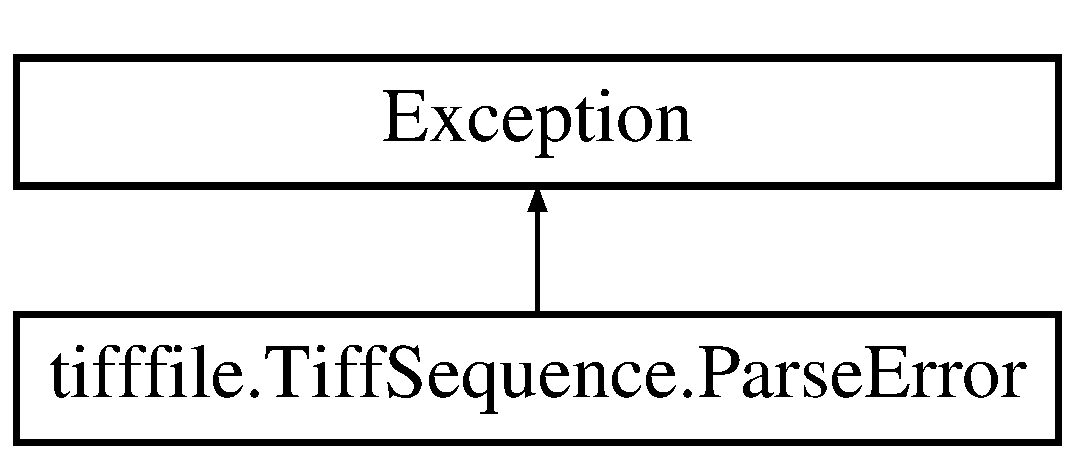
\includegraphics[height=2.000000cm]{classtifffile_1_1_tiff_sequence_1_1_parse_error}
\end{center}
\end{figure}


The documentation for this class was generated from the following file\-:\begin{DoxyCompactItemize}
\item 
workdir/atrex/\-Software/\hyperlink{tifffile_8py}{tifffile.\-py}\end{DoxyCompactItemize}

\hypertarget{classpeak_edit_dlg_1_1peak_edit_dlg}{\section{peak\-Edit\-Dlg.\-peak\-Edit\-Dlg Class Reference}
\label{classpeak_edit_dlg_1_1peak_edit_dlg}\index{peak\-Edit\-Dlg.\-peak\-Edit\-Dlg@{peak\-Edit\-Dlg.\-peak\-Edit\-Dlg}}
}
Inheritance diagram for peak\-Edit\-Dlg.\-peak\-Edit\-Dlg\-:\begin{figure}[H]
\begin{center}
\leavevmode
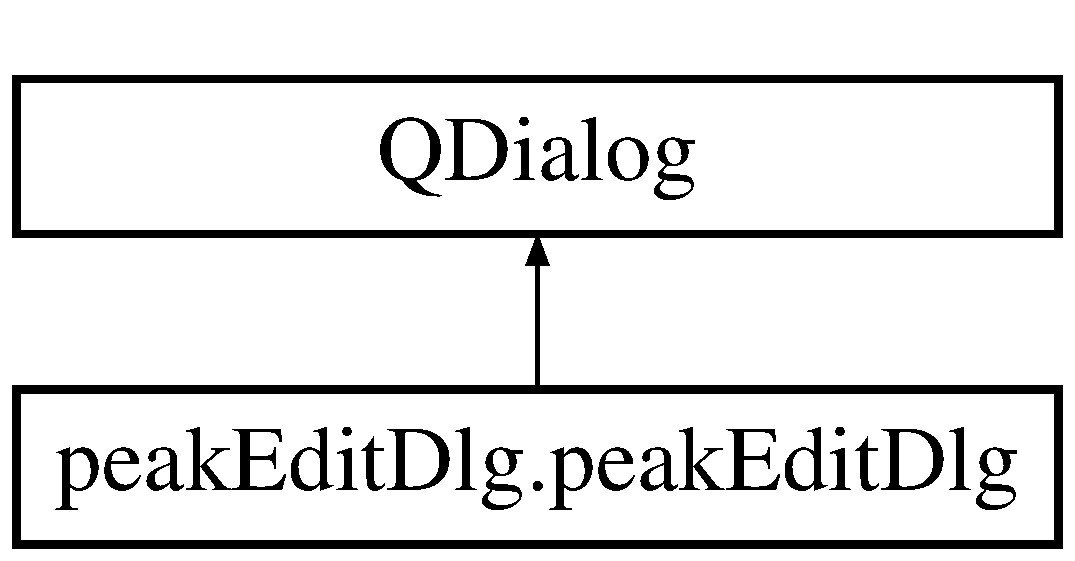
\includegraphics[height=2.000000cm]{classpeak_edit_dlg_1_1peak_edit_dlg}
\end{center}
\end{figure}
\subsection*{Public Member Functions}
\begin{DoxyCompactItemize}
\item 
def \hyperlink{classpeak_edit_dlg_1_1peak_edit_dlg_a3a89be502d41175fb5b75fd419715096}{\-\_\-\-\_\-init\-\_\-\-\_\-}
\item 
def \hyperlink{classpeak_edit_dlg_1_1peak_edit_dlg_ab11967324093e3350fe404fa29e255c1}{set\-Image\-File}
\item 
def \hyperlink{classpeak_edit_dlg_1_1peak_edit_dlg_a2f577ff67c33813f4d803e5d85e62eb2}{text\-Set\-D}
\item 
def \hyperlink{classpeak_edit_dlg_1_1peak_edit_dlg_a2dc064d39d748e09a70a7f6a236c7187}{text\-Set\-F}
\end{DoxyCompactItemize}
\subsection*{Public Attributes}
\begin{DoxyCompactItemize}
\item 
\hyperlink{classpeak_edit_dlg_1_1peak_edit_dlg_a0220ea9f1c4703a47098891c57e1da1f}{ui}
\item 
\hyperlink{classpeak_edit_dlg_1_1peak_edit_dlg_abd94cfb1dd7a9ed84e1955b100a0be78}{peak}
\end{DoxyCompactItemize}


\subsection{Constructor \& Destructor Documentation}
\hypertarget{classpeak_edit_dlg_1_1peak_edit_dlg_a3a89be502d41175fb5b75fd419715096}{\index{peak\-Edit\-Dlg\-::peak\-Edit\-Dlg@{peak\-Edit\-Dlg\-::peak\-Edit\-Dlg}!\-\_\-\-\_\-init\-\_\-\-\_\-@{\-\_\-\-\_\-init\-\_\-\-\_\-}}
\index{\-\_\-\-\_\-init\-\_\-\-\_\-@{\-\_\-\-\_\-init\-\_\-\-\_\-}!peakEditDlg::peakEditDlg@{peak\-Edit\-Dlg\-::peak\-Edit\-Dlg}}
\subsubsection[{\-\_\-\-\_\-init\-\_\-\-\_\-}]{\setlength{\rightskip}{0pt plus 5cm}def peak\-Edit\-Dlg.\-peak\-Edit\-Dlg.\-\_\-\-\_\-init\-\_\-\-\_\- (
\begin{DoxyParamCaption}
\item[{}]{self, }
\item[{}]{peak, }
\item[{}]{rownum}
\end{DoxyParamCaption}
)}}\label{classpeak_edit_dlg_1_1peak_edit_dlg_a3a89be502d41175fb5b75fd419715096}


\subsection{Member Function Documentation}
\hypertarget{classpeak_edit_dlg_1_1peak_edit_dlg_ab11967324093e3350fe404fa29e255c1}{\index{peak\-Edit\-Dlg\-::peak\-Edit\-Dlg@{peak\-Edit\-Dlg\-::peak\-Edit\-Dlg}!set\-Image\-File@{set\-Image\-File}}
\index{set\-Image\-File@{set\-Image\-File}!peakEditDlg::peakEditDlg@{peak\-Edit\-Dlg\-::peak\-Edit\-Dlg}}
\subsubsection[{set\-Image\-File}]{\setlength{\rightskip}{0pt plus 5cm}def peak\-Edit\-Dlg.\-peak\-Edit\-Dlg.\-set\-Image\-File (
\begin{DoxyParamCaption}
\item[{}]{self, }
\item[{}]{imf}
\end{DoxyParamCaption}
)}}\label{classpeak_edit_dlg_1_1peak_edit_dlg_ab11967324093e3350fe404fa29e255c1}
\hypertarget{classpeak_edit_dlg_1_1peak_edit_dlg_a2f577ff67c33813f4d803e5d85e62eb2}{\index{peak\-Edit\-Dlg\-::peak\-Edit\-Dlg@{peak\-Edit\-Dlg\-::peak\-Edit\-Dlg}!text\-Set\-D@{text\-Set\-D}}
\index{text\-Set\-D@{text\-Set\-D}!peakEditDlg::peakEditDlg@{peak\-Edit\-Dlg\-::peak\-Edit\-Dlg}}
\subsubsection[{text\-Set\-D}]{\setlength{\rightskip}{0pt plus 5cm}def peak\-Edit\-Dlg.\-peak\-Edit\-Dlg.\-text\-Set\-D (
\begin{DoxyParamCaption}
\item[{}]{self, }
\item[{}]{L\-E, }
\item[{}]{number}
\end{DoxyParamCaption}
)}}\label{classpeak_edit_dlg_1_1peak_edit_dlg_a2f577ff67c33813f4d803e5d85e62eb2}
\hypertarget{classpeak_edit_dlg_1_1peak_edit_dlg_a2dc064d39d748e09a70a7f6a236c7187}{\index{peak\-Edit\-Dlg\-::peak\-Edit\-Dlg@{peak\-Edit\-Dlg\-::peak\-Edit\-Dlg}!text\-Set\-F@{text\-Set\-F}}
\index{text\-Set\-F@{text\-Set\-F}!peakEditDlg::peakEditDlg@{peak\-Edit\-Dlg\-::peak\-Edit\-Dlg}}
\subsubsection[{text\-Set\-F}]{\setlength{\rightskip}{0pt plus 5cm}def peak\-Edit\-Dlg.\-peak\-Edit\-Dlg.\-text\-Set\-F (
\begin{DoxyParamCaption}
\item[{}]{self, }
\item[{}]{L\-E, }
\item[{}]{number}
\end{DoxyParamCaption}
)}}\label{classpeak_edit_dlg_1_1peak_edit_dlg_a2dc064d39d748e09a70a7f6a236c7187}


\subsection{Member Data Documentation}
\hypertarget{classpeak_edit_dlg_1_1peak_edit_dlg_abd94cfb1dd7a9ed84e1955b100a0be78}{\index{peak\-Edit\-Dlg\-::peak\-Edit\-Dlg@{peak\-Edit\-Dlg\-::peak\-Edit\-Dlg}!peak@{peak}}
\index{peak@{peak}!peakEditDlg::peakEditDlg@{peak\-Edit\-Dlg\-::peak\-Edit\-Dlg}}
\subsubsection[{peak}]{\setlength{\rightskip}{0pt plus 5cm}peak\-Edit\-Dlg.\-peak\-Edit\-Dlg.\-peak}}\label{classpeak_edit_dlg_1_1peak_edit_dlg_abd94cfb1dd7a9ed84e1955b100a0be78}
\hypertarget{classpeak_edit_dlg_1_1peak_edit_dlg_a0220ea9f1c4703a47098891c57e1da1f}{\index{peak\-Edit\-Dlg\-::peak\-Edit\-Dlg@{peak\-Edit\-Dlg\-::peak\-Edit\-Dlg}!ui@{ui}}
\index{ui@{ui}!peakEditDlg::peakEditDlg@{peak\-Edit\-Dlg\-::peak\-Edit\-Dlg}}
\subsubsection[{ui}]{\setlength{\rightskip}{0pt plus 5cm}peak\-Edit\-Dlg.\-peak\-Edit\-Dlg.\-ui}}\label{classpeak_edit_dlg_1_1peak_edit_dlg_a0220ea9f1c4703a47098891c57e1da1f}


The documentation for this class was generated from the following file\-:\begin{DoxyCompactItemize}
\item 
workdir/atrex/\-Software/\hyperlink{peak_edit_dlg_8py}{peak\-Edit\-Dlg.\-py}\end{DoxyCompactItemize}

\hypertarget{classpeak_fit_1_1peak_fit}{\section{peak\-Fit.\-peak\-Fit Class Reference}
\label{classpeak_fit_1_1peak_fit}\index{peak\-Fit.\-peak\-Fit@{peak\-Fit.\-peak\-Fit}}
}
\subsection*{Public Member Functions}
\begin{DoxyCompactItemize}
\item 
def \hyperlink{classpeak_fit_1_1peak_fit_a6ab39ce33c91775176e0c46cc6f936f6}{\-\_\-\-\_\-init\-\_\-\-\_\-}
\item 
def \hyperlink{classpeak_fit_1_1peak_fit_a84a91a33d88ca2403a4e435b5d1f90ec}{fit\-Arr}
\item 
def \hyperlink{classpeak_fit_1_1peak_fit_a0bbfae3ae35fbad87477c06b1607362a}{fit\-Array}
\item 
def \hyperlink{classpeak_fit_1_1peak_fit_a4be5cc7b519e08cd3c401e44449ff06b}{return\-Fit\-Array}
\item 
def \hyperlink{classpeak_fit_1_1peak_fit_ad2af816ebe4e711d783eac36caf062fd}{return\-Fit}
\item 
def \hyperlink{classpeak_fit_1_1peak_fit_a430b52fc42d7539b1374dc4bd1b64efc}{interp\-Array}
\end{DoxyCompactItemize}
\subsection*{Public Attributes}
\begin{DoxyCompactItemize}
\item 
\hyperlink{classpeak_fit_1_1peak_fit_a46bbd242120c1eb44158673fc1ba69eb}{inarr}
\item 
\hyperlink{classpeak_fit_1_1peak_fit_a7bcef9f3d5dbca4a5470a53661dabe4c}{fitpars}
\item 
\hyperlink{classpeak_fit_1_1peak_fit_a1d06c78ecd07718ae71cc50df4d0251c}{fitted}
\end{DoxyCompactItemize}


\subsection{Constructor \& Destructor Documentation}
\hypertarget{classpeak_fit_1_1peak_fit_a6ab39ce33c91775176e0c46cc6f936f6}{\index{peak\-Fit\-::peak\-Fit@{peak\-Fit\-::peak\-Fit}!\-\_\-\-\_\-init\-\_\-\-\_\-@{\-\_\-\-\_\-init\-\_\-\-\_\-}}
\index{\-\_\-\-\_\-init\-\_\-\-\_\-@{\-\_\-\-\_\-init\-\_\-\-\_\-}!peakFit::peakFit@{peak\-Fit\-::peak\-Fit}}
\subsubsection[{\-\_\-\-\_\-init\-\_\-\-\_\-}]{\setlength{\rightskip}{0pt plus 5cm}def peak\-Fit.\-peak\-Fit.\-\_\-\-\_\-init\-\_\-\-\_\- (
\begin{DoxyParamCaption}
\item[{}]{self, }
\item[{}]{arr}
\end{DoxyParamCaption}
)}}\label{classpeak_fit_1_1peak_fit_a6ab39ce33c91775176e0c46cc6f936f6}


\subsection{Member Function Documentation}
\hypertarget{classpeak_fit_1_1peak_fit_a84a91a33d88ca2403a4e435b5d1f90ec}{\index{peak\-Fit\-::peak\-Fit@{peak\-Fit\-::peak\-Fit}!fit\-Arr@{fit\-Arr}}
\index{fit\-Arr@{fit\-Arr}!peakFit::peakFit@{peak\-Fit\-::peak\-Fit}}
\subsubsection[{fit\-Arr}]{\setlength{\rightskip}{0pt plus 5cm}def peak\-Fit.\-peak\-Fit.\-fit\-Arr (
\begin{DoxyParamCaption}
\item[{}]{self}
\end{DoxyParamCaption}
)}}\label{classpeak_fit_1_1peak_fit_a84a91a33d88ca2403a4e435b5d1f90ec}
\hypertarget{classpeak_fit_1_1peak_fit_a0bbfae3ae35fbad87477c06b1607362a}{\index{peak\-Fit\-::peak\-Fit@{peak\-Fit\-::peak\-Fit}!fit\-Array@{fit\-Array}}
\index{fit\-Array@{fit\-Array}!peakFit::peakFit@{peak\-Fit\-::peak\-Fit}}
\subsubsection[{fit\-Array}]{\setlength{\rightskip}{0pt plus 5cm}def peak\-Fit.\-peak\-Fit.\-fit\-Array (
\begin{DoxyParamCaption}
\item[{}]{self, }
\item[{}]{my\-Arr}
\end{DoxyParamCaption}
)}}\label{classpeak_fit_1_1peak_fit_a0bbfae3ae35fbad87477c06b1607362a}
\hypertarget{classpeak_fit_1_1peak_fit_a430b52fc42d7539b1374dc4bd1b64efc}{\index{peak\-Fit\-::peak\-Fit@{peak\-Fit\-::peak\-Fit}!interp\-Array@{interp\-Array}}
\index{interp\-Array@{interp\-Array}!peakFit::peakFit@{peak\-Fit\-::peak\-Fit}}
\subsubsection[{interp\-Array}]{\setlength{\rightskip}{0pt plus 5cm}def peak\-Fit.\-peak\-Fit.\-interp\-Array (
\begin{DoxyParamCaption}
\item[{}]{self, }
\item[{}]{inarr, }
\item[{}]{zmfac}
\end{DoxyParamCaption}
)}}\label{classpeak_fit_1_1peak_fit_a430b52fc42d7539b1374dc4bd1b64efc}
\hypertarget{classpeak_fit_1_1peak_fit_ad2af816ebe4e711d783eac36caf062fd}{\index{peak\-Fit\-::peak\-Fit@{peak\-Fit\-::peak\-Fit}!return\-Fit@{return\-Fit}}
\index{return\-Fit@{return\-Fit}!peakFit::peakFit@{peak\-Fit\-::peak\-Fit}}
\subsubsection[{return\-Fit}]{\setlength{\rightskip}{0pt plus 5cm}def peak\-Fit.\-peak\-Fit.\-return\-Fit (
\begin{DoxyParamCaption}
\item[{}]{self}
\end{DoxyParamCaption}
)}}\label{classpeak_fit_1_1peak_fit_ad2af816ebe4e711d783eac36caf062fd}
\hypertarget{classpeak_fit_1_1peak_fit_a4be5cc7b519e08cd3c401e44449ff06b}{\index{peak\-Fit\-::peak\-Fit@{peak\-Fit\-::peak\-Fit}!return\-Fit\-Array@{return\-Fit\-Array}}
\index{return\-Fit\-Array@{return\-Fit\-Array}!peakFit::peakFit@{peak\-Fit\-::peak\-Fit}}
\subsubsection[{return\-Fit\-Array}]{\setlength{\rightskip}{0pt plus 5cm}def peak\-Fit.\-peak\-Fit.\-return\-Fit\-Array (
\begin{DoxyParamCaption}
\item[{}]{self, }
\item[{}]{my\-Arr}
\end{DoxyParamCaption}
)}}\label{classpeak_fit_1_1peak_fit_a4be5cc7b519e08cd3c401e44449ff06b}


\subsection{Member Data Documentation}
\hypertarget{classpeak_fit_1_1peak_fit_a7bcef9f3d5dbca4a5470a53661dabe4c}{\index{peak\-Fit\-::peak\-Fit@{peak\-Fit\-::peak\-Fit}!fitpars@{fitpars}}
\index{fitpars@{fitpars}!peakFit::peakFit@{peak\-Fit\-::peak\-Fit}}
\subsubsection[{fitpars}]{\setlength{\rightskip}{0pt plus 5cm}peak\-Fit.\-peak\-Fit.\-fitpars}}\label{classpeak_fit_1_1peak_fit_a7bcef9f3d5dbca4a5470a53661dabe4c}
\hypertarget{classpeak_fit_1_1peak_fit_a1d06c78ecd07718ae71cc50df4d0251c}{\index{peak\-Fit\-::peak\-Fit@{peak\-Fit\-::peak\-Fit}!fitted@{fitted}}
\index{fitted@{fitted}!peakFit::peakFit@{peak\-Fit\-::peak\-Fit}}
\subsubsection[{fitted}]{\setlength{\rightskip}{0pt plus 5cm}peak\-Fit.\-peak\-Fit.\-fitted}}\label{classpeak_fit_1_1peak_fit_a1d06c78ecd07718ae71cc50df4d0251c}
\hypertarget{classpeak_fit_1_1peak_fit_a46bbd242120c1eb44158673fc1ba69eb}{\index{peak\-Fit\-::peak\-Fit@{peak\-Fit\-::peak\-Fit}!inarr@{inarr}}
\index{inarr@{inarr}!peakFit::peakFit@{peak\-Fit\-::peak\-Fit}}
\subsubsection[{inarr}]{\setlength{\rightskip}{0pt plus 5cm}peak\-Fit.\-peak\-Fit.\-inarr}}\label{classpeak_fit_1_1peak_fit_a46bbd242120c1eb44158673fc1ba69eb}


The documentation for this class was generated from the following file\-:\begin{DoxyCompactItemize}
\item 
workdir/atrex/\-Software/\hyperlink{peak_fit_8py}{peak\-Fit.\-py}\end{DoxyCompactItemize}

\hypertarget{class_peak_object_1_1_peak_object}{\section{Peak\-Object.\-Peak\-Object Class Reference}
\label{class_peak_object_1_1_peak_object}\index{Peak\-Object.\-Peak\-Object@{Peak\-Object.\-Peak\-Object}}
}
\subsection*{Public Member Functions}
\begin{DoxyCompactItemize}
\item 
def \hyperlink{class_peak_object_1_1_peak_object_a066c72d23958912081182a5aca95e32c}{\-\_\-\-\_\-init\-\_\-\-\_\-}
\item 
def \hyperlink{class_peak_object_1_1_peak_object_a44e1f82c79582b10885050ae8ffd7201}{x}
\item 
def \hyperlink{class_peak_object_1_1_peak_object_a674a319850462abc76a7091e49c2425c}{y}
\item 
def \hyperlink{class_peak_object_1_1_peak_object_a4a9dabf7ebe3b0703da235f77259d5d2}{set\-Selected}
\end{DoxyCompactItemize}
\subsection*{Public Attributes}
\begin{DoxyCompactItemize}
\item 
\hyperlink{class_peak_object_1_1_peak_object_a0675bfef330cb0e7111c507d0fd2f505}{xloc}
\item 
\hyperlink{class_peak_object_1_1_peak_object_adc5441b9bde0d002725032741bce8a3a}{yloc}
\end{DoxyCompactItemize}
\subsection*{Static Public Attributes}
\begin{DoxyCompactItemize}
\item 
int \hyperlink{class_peak_object_1_1_peak_object_a547374a82aab09bcf28e13ecfb598117}{xloc} = 0
\item 
int \hyperlink{class_peak_object_1_1_peak_object_abebfb4985f9b0b73e6b1e20cb5a56f18}{yloc} = 0
\item 
tuple \hyperlink{class_peak_object_1_1_peak_object_a5d69241780c9ba49bccd1a76c3ef2738}{ident} = Qt\-Core.\-Q\-String(\char`\"{}\char`\"{})
\item 
\hyperlink{class_peak_object_1_1_peak_object_aa0095eabde0eeb9ed146a052f7dea921}{selected} = False
\end{DoxyCompactItemize}


\subsection{Constructor \& Destructor Documentation}
\hypertarget{class_peak_object_1_1_peak_object_a066c72d23958912081182a5aca95e32c}{\index{Peak\-Object\-::\-Peak\-Object@{Peak\-Object\-::\-Peak\-Object}!\-\_\-\-\_\-init\-\_\-\-\_\-@{\-\_\-\-\_\-init\-\_\-\-\_\-}}
\index{\-\_\-\-\_\-init\-\_\-\-\_\-@{\-\_\-\-\_\-init\-\_\-\-\_\-}!PeakObject::PeakObject@{Peak\-Object\-::\-Peak\-Object}}
\subsubsection[{\-\_\-\-\_\-init\-\_\-\-\_\-}]{\setlength{\rightskip}{0pt plus 5cm}def Peak\-Object.\-Peak\-Object.\-\_\-\-\_\-init\-\_\-\-\_\- (
\begin{DoxyParamCaption}
\item[{}]{self, }
\item[{}]{x, }
\item[{}]{y}
\end{DoxyParamCaption}
)}}\label{class_peak_object_1_1_peak_object_a066c72d23958912081182a5aca95e32c}


\subsection{Member Function Documentation}
\hypertarget{class_peak_object_1_1_peak_object_a4a9dabf7ebe3b0703da235f77259d5d2}{\index{Peak\-Object\-::\-Peak\-Object@{Peak\-Object\-::\-Peak\-Object}!set\-Selected@{set\-Selected}}
\index{set\-Selected@{set\-Selected}!PeakObject::PeakObject@{Peak\-Object\-::\-Peak\-Object}}
\subsubsection[{set\-Selected}]{\setlength{\rightskip}{0pt plus 5cm}def Peak\-Object.\-Peak\-Object.\-set\-Selected (
\begin{DoxyParamCaption}
\item[{}]{self, }
\item[{}]{state}
\end{DoxyParamCaption}
)}}\label{class_peak_object_1_1_peak_object_a4a9dabf7ebe3b0703da235f77259d5d2}
\hypertarget{class_peak_object_1_1_peak_object_a44e1f82c79582b10885050ae8ffd7201}{\index{Peak\-Object\-::\-Peak\-Object@{Peak\-Object\-::\-Peak\-Object}!x@{x}}
\index{x@{x}!PeakObject::PeakObject@{Peak\-Object\-::\-Peak\-Object}}
\subsubsection[{x}]{\setlength{\rightskip}{0pt plus 5cm}def Peak\-Object.\-Peak\-Object.\-x (
\begin{DoxyParamCaption}
\item[{}]{self}
\end{DoxyParamCaption}
)}}\label{class_peak_object_1_1_peak_object_a44e1f82c79582b10885050ae8ffd7201}
\hypertarget{class_peak_object_1_1_peak_object_a674a319850462abc76a7091e49c2425c}{\index{Peak\-Object\-::\-Peak\-Object@{Peak\-Object\-::\-Peak\-Object}!y@{y}}
\index{y@{y}!PeakObject::PeakObject@{Peak\-Object\-::\-Peak\-Object}}
\subsubsection[{y}]{\setlength{\rightskip}{0pt plus 5cm}def Peak\-Object.\-Peak\-Object.\-y (
\begin{DoxyParamCaption}
\item[{}]{self}
\end{DoxyParamCaption}
)}}\label{class_peak_object_1_1_peak_object_a674a319850462abc76a7091e49c2425c}


\subsection{Member Data Documentation}
\hypertarget{class_peak_object_1_1_peak_object_a5d69241780c9ba49bccd1a76c3ef2738}{\index{Peak\-Object\-::\-Peak\-Object@{Peak\-Object\-::\-Peak\-Object}!ident@{ident}}
\index{ident@{ident}!PeakObject::PeakObject@{Peak\-Object\-::\-Peak\-Object}}
\subsubsection[{ident}]{\setlength{\rightskip}{0pt plus 5cm}tuple Peak\-Object.\-Peak\-Object.\-ident = Qt\-Core.\-Q\-String(\char`\"{}\char`\"{})\hspace{0.3cm}{\ttfamily [static]}}}\label{class_peak_object_1_1_peak_object_a5d69241780c9ba49bccd1a76c3ef2738}
\hypertarget{class_peak_object_1_1_peak_object_aa0095eabde0eeb9ed146a052f7dea921}{\index{Peak\-Object\-::\-Peak\-Object@{Peak\-Object\-::\-Peak\-Object}!selected@{selected}}
\index{selected@{selected}!PeakObject::PeakObject@{Peak\-Object\-::\-Peak\-Object}}
\subsubsection[{selected}]{\setlength{\rightskip}{0pt plus 5cm}Peak\-Object.\-Peak\-Object.\-selected = False\hspace{0.3cm}{\ttfamily [static]}}}\label{class_peak_object_1_1_peak_object_aa0095eabde0eeb9ed146a052f7dea921}
\hypertarget{class_peak_object_1_1_peak_object_a547374a82aab09bcf28e13ecfb598117}{\index{Peak\-Object\-::\-Peak\-Object@{Peak\-Object\-::\-Peak\-Object}!xloc@{xloc}}
\index{xloc@{xloc}!PeakObject::PeakObject@{Peak\-Object\-::\-Peak\-Object}}
\subsubsection[{xloc}]{\setlength{\rightskip}{0pt plus 5cm}int Peak\-Object.\-Peak\-Object.\-xloc = 0\hspace{0.3cm}{\ttfamily [static]}}}\label{class_peak_object_1_1_peak_object_a547374a82aab09bcf28e13ecfb598117}
\hypertarget{class_peak_object_1_1_peak_object_a0675bfef330cb0e7111c507d0fd2f505}{\index{Peak\-Object\-::\-Peak\-Object@{Peak\-Object\-::\-Peak\-Object}!xloc@{xloc}}
\index{xloc@{xloc}!PeakObject::PeakObject@{Peak\-Object\-::\-Peak\-Object}}
\subsubsection[{xloc}]{\setlength{\rightskip}{0pt plus 5cm}Peak\-Object.\-Peak\-Object.\-xloc}}\label{class_peak_object_1_1_peak_object_a0675bfef330cb0e7111c507d0fd2f505}
\hypertarget{class_peak_object_1_1_peak_object_abebfb4985f9b0b73e6b1e20cb5a56f18}{\index{Peak\-Object\-::\-Peak\-Object@{Peak\-Object\-::\-Peak\-Object}!yloc@{yloc}}
\index{yloc@{yloc}!PeakObject::PeakObject@{Peak\-Object\-::\-Peak\-Object}}
\subsubsection[{yloc}]{\setlength{\rightskip}{0pt plus 5cm}int Peak\-Object.\-Peak\-Object.\-yloc = 0\hspace{0.3cm}{\ttfamily [static]}}}\label{class_peak_object_1_1_peak_object_abebfb4985f9b0b73e6b1e20cb5a56f18}
\hypertarget{class_peak_object_1_1_peak_object_adc5441b9bde0d002725032741bce8a3a}{\index{Peak\-Object\-::\-Peak\-Object@{Peak\-Object\-::\-Peak\-Object}!yloc@{yloc}}
\index{yloc@{yloc}!PeakObject::PeakObject@{Peak\-Object\-::\-Peak\-Object}}
\subsubsection[{yloc}]{\setlength{\rightskip}{0pt plus 5cm}Peak\-Object.\-Peak\-Object.\-yloc}}\label{class_peak_object_1_1_peak_object_adc5441b9bde0d002725032741bce8a3a}


The documentation for this class was generated from the following file\-:\begin{DoxyCompactItemize}
\item 
workdir/atrex/\-Software/\hyperlink{_peak_object_8py}{Peak\-Object.\-py}\end{DoxyCompactItemize}

\hypertarget{class_project_1_1_project}{\section{Project.\-Project Class Reference}
\label{class_project_1_1_project}\index{Project.\-Project@{Project.\-Project}}
}
\subsection*{Public Member Functions}
\begin{DoxyCompactItemize}
\item 
def \hyperlink{class_project_1_1_project_af5d15337a24279fed5df943cdd17a521}{get\-Image\-Base}
\item 
def \hyperlink{class_project_1_1_project_af4f0a9adbac70beed61838e0552b5fce}{get\-File\-Name\-From\-Num}
\item 
def \hyperlink{class_project_1_1_project_a26e3cfe3e056c97f722eeef03137c475}{get\-File\-Number}
\item 
def \hyperlink{class_project_1_1_project_aa4241d0e834f8686b89e977ad6b16d26}{check\-For\-Files}
\item 
def \hyperlink{class_project_1_1_project_abcb28ed447f9094e8eb6d6a49b0c4294}{read\-File\-Settings}
\item 
def \hyperlink{class_project_1_1_project_a4b58bd09e8457006fb81aa85d7723a7d}{write\-Settings\-Files}
\end{DoxyCompactItemize}
\subsection*{Public Attributes}
\begin{DoxyCompactItemize}
\item 
\hyperlink{class_project_1_1_project_aec70e48d90635d6c41b66660fc23c14b}{im\-File}
\item 
\hyperlink{class_project_1_1_project_a4a1a26e41d50eafb9a1ecd7c344ae974}{base}
\item 
\hyperlink{class_project_1_1_project_ae8e5eb7ce2196fd5eec5b91686732069}{filenum}
\item 
\hyperlink{class_project_1_1_project_abf36ec5e3005385e03d533200b5c098a}{num\-Digits}
\item 
\hyperlink{class_project_1_1_project_af03d34654b00a3f4d1f8a38b834af406}{min\-Image\-Num}
\item 
\hyperlink{class_project_1_1_project_afc5b3afcc2020e4527c6328c508ad5c9}{max\-Image\-Num}
\item 
\hyperlink{class_project_1_1_project_aed74c6fd1832b33e1299f1180a691fa6}{prj\-File}
\item 
\hyperlink{class_project_1_1_project_a8eae8faddab323b07537ca6a5f3916cc}{ub\-File}
\item 
\hyperlink{class_project_1_1_project_ae2e3e43c456a03959ddc60f010e54aa9}{omega0}
\item 
\hyperlink{class_project_1_1_project_a05d50a418a51ea0f4dcf7d1a87812b00}{omega\-R}
\item 
\hyperlink{class_project_1_1_project_aae1d33efbce822c8023528ff7f3b841a}{chi}
\item 
\hyperlink{class_project_1_1_project_a2513615e3adc838e60e00da5c77ef307}{detector}
\item 
\hyperlink{class_project_1_1_project_aa53e83e0b9b4b05e86bbb6b80873d700}{expos}
\end{DoxyCompactItemize}
\subsection*{Static Public Attributes}
\begin{DoxyCompactItemize}
\item 
string \hyperlink{class_project_1_1_project_a3fa761a117618c8524b700ceb2c7122f}{base} = ''
\item 
int \hyperlink{class_project_1_1_project_a9294abcb712f449838e46b3e98aa74f1}{filenum} = 0
\item 
tuple \hyperlink{class_project_1_1_project_aa523085a77fa7d77f1e8112dc95aa35b}{curimage} = Qt\-Core.\-Q\-String('')
\item 
\hyperlink{class_project_1_1_project_a24e1a52b21994951813562a80bfcdcad}{proj\-Flag} = False
\item 
\hyperlink{class_project_1_1_project_ad80180beff6260cee514b29e80083d55}{ub\-Flag} = False
\item 
string \hyperlink{class_project_1_1_project_aa2118a5e8c2024d900ce4cecf8d0bc5b}{proj\-File} = ''
\item 
string \hyperlink{class_project_1_1_project_add56cb764f050d4cbd41564b5de6bdf0}{ub\-File} = ''
\item 
list \hyperlink{class_project_1_1_project_a0d645f784cc44f878dc6bbaf86579517}{settings\-Array} = \mbox{[}0.,0.,0.,0.,0.,0.,0\mbox{]}
\item 
int \hyperlink{class_project_1_1_project_a441402412f2536707678ddc504873b29}{num\-Digits} = 3
\item 
int \hyperlink{class_project_1_1_project_a08ab65a606b424f1c03e20fc87df6907}{min\-Image\-Num} = 1
\item 
int \hyperlink{class_project_1_1_project_a4a71b55b2b2893cfa10f8375b75aab14}{max\-Image\-Num} = -\/1
\item 
string \hyperlink{class_project_1_1_project_ac2e36746ec209c56d0609cc99a0bc138}{im\-File} = ''
\item 
int \hyperlink{class_project_1_1_project_a5a62c4d934e7182c36b4f50bd590b29a}{omega0} = 0
\item 
int \hyperlink{class_project_1_1_project_ae5bb0d5790b39c1ba5185ee7cfdd6a0a}{omega\-R} = 15
\item 
int \hyperlink{class_project_1_1_project_a7f1d473c7f6210a62aca3991c0c3acc9}{expos} = 10
\item 
int \hyperlink{class_project_1_1_project_a2b04fbe0238d23490f6482a17046da9a}{chi} = 0
\item 
int \hyperlink{class_project_1_1_project_a51202b77e720d7d2c68c62ee982c372e}{detector} = 0
\end{DoxyCompactItemize}


\subsection{Detailed Description}
\begin{DoxyVerb}Project.py
Class containing utilities to get the image base from a input file name and to return a filename
based upon the image base
\end{DoxyVerb}
 

\subsection{Member Function Documentation}
\hypertarget{class_project_1_1_project_aa4241d0e834f8686b89e977ad6b16d26}{\index{Project\-::\-Project@{Project\-::\-Project}!check\-For\-Files@{check\-For\-Files}}
\index{check\-For\-Files@{check\-For\-Files}!Project::Project@{Project\-::\-Project}}
\subsubsection[{check\-For\-Files}]{\setlength{\rightskip}{0pt plus 5cm}def Project.\-Project.\-check\-For\-Files (
\begin{DoxyParamCaption}
\item[{}]{self}
\end{DoxyParamCaption}
)}}\label{class_project_1_1_project_aa4241d0e834f8686b89e977ad6b16d26}
\hypertarget{class_project_1_1_project_af4f0a9adbac70beed61838e0552b5fce}{\index{Project\-::\-Project@{Project\-::\-Project}!get\-File\-Name\-From\-Num@{get\-File\-Name\-From\-Num}}
\index{get\-File\-Name\-From\-Num@{get\-File\-Name\-From\-Num}!Project::Project@{Project\-::\-Project}}
\subsubsection[{get\-File\-Name\-From\-Num}]{\setlength{\rightskip}{0pt plus 5cm}def Project.\-Project.\-get\-File\-Name\-From\-Num (
\begin{DoxyParamCaption}
\item[{}]{self, }
\item[{}]{number}
\end{DoxyParamCaption}
)}}\label{class_project_1_1_project_af4f0a9adbac70beed61838e0552b5fce}
\hypertarget{class_project_1_1_project_a26e3cfe3e056c97f722eeef03137c475}{\index{Project\-::\-Project@{Project\-::\-Project}!get\-File\-Number@{get\-File\-Number}}
\index{get\-File\-Number@{get\-File\-Number}!Project::Project@{Project\-::\-Project}}
\subsubsection[{get\-File\-Number}]{\setlength{\rightskip}{0pt plus 5cm}def Project.\-Project.\-get\-File\-Number (
\begin{DoxyParamCaption}
\item[{}]{self, }
\item[{}]{filename}
\end{DoxyParamCaption}
)}}\label{class_project_1_1_project_a26e3cfe3e056c97f722eeef03137c475}
\hypertarget{class_project_1_1_project_af5d15337a24279fed5df943cdd17a521}{\index{Project\-::\-Project@{Project\-::\-Project}!get\-Image\-Base@{get\-Image\-Base}}
\index{get\-Image\-Base@{get\-Image\-Base}!Project::Project@{Project\-::\-Project}}
\subsubsection[{get\-Image\-Base}]{\setlength{\rightskip}{0pt plus 5cm}def Project.\-Project.\-get\-Image\-Base (
\begin{DoxyParamCaption}
\item[{}]{self, }
\item[{}]{filename}
\end{DoxyParamCaption}
)}}\label{class_project_1_1_project_af5d15337a24279fed5df943cdd17a521}
\begin{DoxyVerb}getImageBase returns the prefix which will be used for subsequent file naming based upon
an input filename
:param filename:
:return:
\end{DoxyVerb}
 \hypertarget{class_project_1_1_project_abcb28ed447f9094e8eb6d6a49b0c4294}{\index{Project\-::\-Project@{Project\-::\-Project}!read\-File\-Settings@{read\-File\-Settings}}
\index{read\-File\-Settings@{read\-File\-Settings}!Project::Project@{Project\-::\-Project}}
\subsubsection[{read\-File\-Settings}]{\setlength{\rightskip}{0pt plus 5cm}def Project.\-Project.\-read\-File\-Settings (
\begin{DoxyParamCaption}
\item[{}]{self, }
\item[{}]{fname}
\end{DoxyParamCaption}
)}}\label{class_project_1_1_project_abcb28ed447f9094e8eb6d6a49b0c4294}
\hypertarget{class_project_1_1_project_a4b58bd09e8457006fb81aa85d7723a7d}{\index{Project\-::\-Project@{Project\-::\-Project}!write\-Settings\-Files@{write\-Settings\-Files}}
\index{write\-Settings\-Files@{write\-Settings\-Files}!Project::Project@{Project\-::\-Project}}
\subsubsection[{write\-Settings\-Files}]{\setlength{\rightskip}{0pt plus 5cm}def Project.\-Project.\-write\-Settings\-Files (
\begin{DoxyParamCaption}
\item[{}]{self}
\end{DoxyParamCaption}
)}}\label{class_project_1_1_project_a4b58bd09e8457006fb81aa85d7723a7d}


\subsection{Member Data Documentation}
\hypertarget{class_project_1_1_project_a3fa761a117618c8524b700ceb2c7122f}{\index{Project\-::\-Project@{Project\-::\-Project}!base@{base}}
\index{base@{base}!Project::Project@{Project\-::\-Project}}
\subsubsection[{base}]{\setlength{\rightskip}{0pt plus 5cm}string Project.\-Project.\-base = ''\hspace{0.3cm}{\ttfamily [static]}}}\label{class_project_1_1_project_a3fa761a117618c8524b700ceb2c7122f}
\hypertarget{class_project_1_1_project_a4a1a26e41d50eafb9a1ecd7c344ae974}{\index{Project\-::\-Project@{Project\-::\-Project}!base@{base}}
\index{base@{base}!Project::Project@{Project\-::\-Project}}
\subsubsection[{base}]{\setlength{\rightskip}{0pt plus 5cm}Project.\-Project.\-base}}\label{class_project_1_1_project_a4a1a26e41d50eafb9a1ecd7c344ae974}
\hypertarget{class_project_1_1_project_a2b04fbe0238d23490f6482a17046da9a}{\index{Project\-::\-Project@{Project\-::\-Project}!chi@{chi}}
\index{chi@{chi}!Project::Project@{Project\-::\-Project}}
\subsubsection[{chi}]{\setlength{\rightskip}{0pt plus 5cm}int Project.\-Project.\-chi = 0\hspace{0.3cm}{\ttfamily [static]}}}\label{class_project_1_1_project_a2b04fbe0238d23490f6482a17046da9a}
\hypertarget{class_project_1_1_project_aae1d33efbce822c8023528ff7f3b841a}{\index{Project\-::\-Project@{Project\-::\-Project}!chi@{chi}}
\index{chi@{chi}!Project::Project@{Project\-::\-Project}}
\subsubsection[{chi}]{\setlength{\rightskip}{0pt plus 5cm}Project.\-Project.\-chi}}\label{class_project_1_1_project_aae1d33efbce822c8023528ff7f3b841a}
\hypertarget{class_project_1_1_project_aa523085a77fa7d77f1e8112dc95aa35b}{\index{Project\-::\-Project@{Project\-::\-Project}!curimage@{curimage}}
\index{curimage@{curimage}!Project::Project@{Project\-::\-Project}}
\subsubsection[{curimage}]{\setlength{\rightskip}{0pt plus 5cm}tuple Project.\-Project.\-curimage = Qt\-Core.\-Q\-String('')\hspace{0.3cm}{\ttfamily [static]}}}\label{class_project_1_1_project_aa523085a77fa7d77f1e8112dc95aa35b}
\hypertarget{class_project_1_1_project_a51202b77e720d7d2c68c62ee982c372e}{\index{Project\-::\-Project@{Project\-::\-Project}!detector@{detector}}
\index{detector@{detector}!Project::Project@{Project\-::\-Project}}
\subsubsection[{detector}]{\setlength{\rightskip}{0pt plus 5cm}int Project.\-Project.\-detector = 0\hspace{0.3cm}{\ttfamily [static]}}}\label{class_project_1_1_project_a51202b77e720d7d2c68c62ee982c372e}
\hypertarget{class_project_1_1_project_a2513615e3adc838e60e00da5c77ef307}{\index{Project\-::\-Project@{Project\-::\-Project}!detector@{detector}}
\index{detector@{detector}!Project::Project@{Project\-::\-Project}}
\subsubsection[{detector}]{\setlength{\rightskip}{0pt plus 5cm}Project.\-Project.\-detector}}\label{class_project_1_1_project_a2513615e3adc838e60e00da5c77ef307}
\hypertarget{class_project_1_1_project_a7f1d473c7f6210a62aca3991c0c3acc9}{\index{Project\-::\-Project@{Project\-::\-Project}!expos@{expos}}
\index{expos@{expos}!Project::Project@{Project\-::\-Project}}
\subsubsection[{expos}]{\setlength{\rightskip}{0pt plus 5cm}int Project.\-Project.\-expos = 10\hspace{0.3cm}{\ttfamily [static]}}}\label{class_project_1_1_project_a7f1d473c7f6210a62aca3991c0c3acc9}
\hypertarget{class_project_1_1_project_aa53e83e0b9b4b05e86bbb6b80873d700}{\index{Project\-::\-Project@{Project\-::\-Project}!expos@{expos}}
\index{expos@{expos}!Project::Project@{Project\-::\-Project}}
\subsubsection[{expos}]{\setlength{\rightskip}{0pt plus 5cm}Project.\-Project.\-expos}}\label{class_project_1_1_project_aa53e83e0b9b4b05e86bbb6b80873d700}
\hypertarget{class_project_1_1_project_a9294abcb712f449838e46b3e98aa74f1}{\index{Project\-::\-Project@{Project\-::\-Project}!filenum@{filenum}}
\index{filenum@{filenum}!Project::Project@{Project\-::\-Project}}
\subsubsection[{filenum}]{\setlength{\rightskip}{0pt plus 5cm}int Project.\-Project.\-filenum = 0\hspace{0.3cm}{\ttfamily [static]}}}\label{class_project_1_1_project_a9294abcb712f449838e46b3e98aa74f1}
\hypertarget{class_project_1_1_project_ae8e5eb7ce2196fd5eec5b91686732069}{\index{Project\-::\-Project@{Project\-::\-Project}!filenum@{filenum}}
\index{filenum@{filenum}!Project::Project@{Project\-::\-Project}}
\subsubsection[{filenum}]{\setlength{\rightskip}{0pt plus 5cm}Project.\-Project.\-filenum}}\label{class_project_1_1_project_ae8e5eb7ce2196fd5eec5b91686732069}
\hypertarget{class_project_1_1_project_ac2e36746ec209c56d0609cc99a0bc138}{\index{Project\-::\-Project@{Project\-::\-Project}!im\-File@{im\-File}}
\index{im\-File@{im\-File}!Project::Project@{Project\-::\-Project}}
\subsubsection[{im\-File}]{\setlength{\rightskip}{0pt plus 5cm}string Project.\-Project.\-im\-File = ''\hspace{0.3cm}{\ttfamily [static]}}}\label{class_project_1_1_project_ac2e36746ec209c56d0609cc99a0bc138}
\hypertarget{class_project_1_1_project_aec70e48d90635d6c41b66660fc23c14b}{\index{Project\-::\-Project@{Project\-::\-Project}!im\-File@{im\-File}}
\index{im\-File@{im\-File}!Project::Project@{Project\-::\-Project}}
\subsubsection[{im\-File}]{\setlength{\rightskip}{0pt plus 5cm}Project.\-Project.\-im\-File}}\label{class_project_1_1_project_aec70e48d90635d6c41b66660fc23c14b}
\hypertarget{class_project_1_1_project_a4a71b55b2b2893cfa10f8375b75aab14}{\index{Project\-::\-Project@{Project\-::\-Project}!max\-Image\-Num@{max\-Image\-Num}}
\index{max\-Image\-Num@{max\-Image\-Num}!Project::Project@{Project\-::\-Project}}
\subsubsection[{max\-Image\-Num}]{\setlength{\rightskip}{0pt plus 5cm}int Project.\-Project.\-max\-Image\-Num = -\/1\hspace{0.3cm}{\ttfamily [static]}}}\label{class_project_1_1_project_a4a71b55b2b2893cfa10f8375b75aab14}
\hypertarget{class_project_1_1_project_afc5b3afcc2020e4527c6328c508ad5c9}{\index{Project\-::\-Project@{Project\-::\-Project}!max\-Image\-Num@{max\-Image\-Num}}
\index{max\-Image\-Num@{max\-Image\-Num}!Project::Project@{Project\-::\-Project}}
\subsubsection[{max\-Image\-Num}]{\setlength{\rightskip}{0pt plus 5cm}Project.\-Project.\-max\-Image\-Num}}\label{class_project_1_1_project_afc5b3afcc2020e4527c6328c508ad5c9}
\hypertarget{class_project_1_1_project_a08ab65a606b424f1c03e20fc87df6907}{\index{Project\-::\-Project@{Project\-::\-Project}!min\-Image\-Num@{min\-Image\-Num}}
\index{min\-Image\-Num@{min\-Image\-Num}!Project::Project@{Project\-::\-Project}}
\subsubsection[{min\-Image\-Num}]{\setlength{\rightskip}{0pt plus 5cm}int Project.\-Project.\-min\-Image\-Num = 1\hspace{0.3cm}{\ttfamily [static]}}}\label{class_project_1_1_project_a08ab65a606b424f1c03e20fc87df6907}
\hypertarget{class_project_1_1_project_af03d34654b00a3f4d1f8a38b834af406}{\index{Project\-::\-Project@{Project\-::\-Project}!min\-Image\-Num@{min\-Image\-Num}}
\index{min\-Image\-Num@{min\-Image\-Num}!Project::Project@{Project\-::\-Project}}
\subsubsection[{min\-Image\-Num}]{\setlength{\rightskip}{0pt plus 5cm}Project.\-Project.\-min\-Image\-Num}}\label{class_project_1_1_project_af03d34654b00a3f4d1f8a38b834af406}
\hypertarget{class_project_1_1_project_a441402412f2536707678ddc504873b29}{\index{Project\-::\-Project@{Project\-::\-Project}!num\-Digits@{num\-Digits}}
\index{num\-Digits@{num\-Digits}!Project::Project@{Project\-::\-Project}}
\subsubsection[{num\-Digits}]{\setlength{\rightskip}{0pt plus 5cm}int Project.\-Project.\-num\-Digits = 3\hspace{0.3cm}{\ttfamily [static]}}}\label{class_project_1_1_project_a441402412f2536707678ddc504873b29}
\hypertarget{class_project_1_1_project_abf36ec5e3005385e03d533200b5c098a}{\index{Project\-::\-Project@{Project\-::\-Project}!num\-Digits@{num\-Digits}}
\index{num\-Digits@{num\-Digits}!Project::Project@{Project\-::\-Project}}
\subsubsection[{num\-Digits}]{\setlength{\rightskip}{0pt plus 5cm}Project.\-Project.\-num\-Digits}}\label{class_project_1_1_project_abf36ec5e3005385e03d533200b5c098a}
\hypertarget{class_project_1_1_project_a5a62c4d934e7182c36b4f50bd590b29a}{\index{Project\-::\-Project@{Project\-::\-Project}!omega0@{omega0}}
\index{omega0@{omega0}!Project::Project@{Project\-::\-Project}}
\subsubsection[{omega0}]{\setlength{\rightskip}{0pt plus 5cm}int Project.\-Project.\-omega0 = 0\hspace{0.3cm}{\ttfamily [static]}}}\label{class_project_1_1_project_a5a62c4d934e7182c36b4f50bd590b29a}
\hypertarget{class_project_1_1_project_ae2e3e43c456a03959ddc60f010e54aa9}{\index{Project\-::\-Project@{Project\-::\-Project}!omega0@{omega0}}
\index{omega0@{omega0}!Project::Project@{Project\-::\-Project}}
\subsubsection[{omega0}]{\setlength{\rightskip}{0pt plus 5cm}Project.\-Project.\-omega0}}\label{class_project_1_1_project_ae2e3e43c456a03959ddc60f010e54aa9}
\hypertarget{class_project_1_1_project_ae5bb0d5790b39c1ba5185ee7cfdd6a0a}{\index{Project\-::\-Project@{Project\-::\-Project}!omega\-R@{omega\-R}}
\index{omega\-R@{omega\-R}!Project::Project@{Project\-::\-Project}}
\subsubsection[{omega\-R}]{\setlength{\rightskip}{0pt plus 5cm}int Project.\-Project.\-omega\-R = 15\hspace{0.3cm}{\ttfamily [static]}}}\label{class_project_1_1_project_ae5bb0d5790b39c1ba5185ee7cfdd6a0a}
\hypertarget{class_project_1_1_project_a05d50a418a51ea0f4dcf7d1a87812b00}{\index{Project\-::\-Project@{Project\-::\-Project}!omega\-R@{omega\-R}}
\index{omega\-R@{omega\-R}!Project::Project@{Project\-::\-Project}}
\subsubsection[{omega\-R}]{\setlength{\rightskip}{0pt plus 5cm}Project.\-Project.\-omega\-R}}\label{class_project_1_1_project_a05d50a418a51ea0f4dcf7d1a87812b00}
\hypertarget{class_project_1_1_project_aed74c6fd1832b33e1299f1180a691fa6}{\index{Project\-::\-Project@{Project\-::\-Project}!prj\-File@{prj\-File}}
\index{prj\-File@{prj\-File}!Project::Project@{Project\-::\-Project}}
\subsubsection[{prj\-File}]{\setlength{\rightskip}{0pt plus 5cm}Project.\-Project.\-prj\-File}}\label{class_project_1_1_project_aed74c6fd1832b33e1299f1180a691fa6}
\hypertarget{class_project_1_1_project_aa2118a5e8c2024d900ce4cecf8d0bc5b}{\index{Project\-::\-Project@{Project\-::\-Project}!proj\-File@{proj\-File}}
\index{proj\-File@{proj\-File}!Project::Project@{Project\-::\-Project}}
\subsubsection[{proj\-File}]{\setlength{\rightskip}{0pt plus 5cm}string Project.\-Project.\-proj\-File = ''\hspace{0.3cm}{\ttfamily [static]}}}\label{class_project_1_1_project_aa2118a5e8c2024d900ce4cecf8d0bc5b}
\hypertarget{class_project_1_1_project_a24e1a52b21994951813562a80bfcdcad}{\index{Project\-::\-Project@{Project\-::\-Project}!proj\-Flag@{proj\-Flag}}
\index{proj\-Flag@{proj\-Flag}!Project::Project@{Project\-::\-Project}}
\subsubsection[{proj\-Flag}]{\setlength{\rightskip}{0pt plus 5cm}Project.\-Project.\-proj\-Flag = False\hspace{0.3cm}{\ttfamily [static]}}}\label{class_project_1_1_project_a24e1a52b21994951813562a80bfcdcad}
\hypertarget{class_project_1_1_project_a0d645f784cc44f878dc6bbaf86579517}{\index{Project\-::\-Project@{Project\-::\-Project}!settings\-Array@{settings\-Array}}
\index{settings\-Array@{settings\-Array}!Project::Project@{Project\-::\-Project}}
\subsubsection[{settings\-Array}]{\setlength{\rightskip}{0pt plus 5cm}list Project.\-Project.\-settings\-Array = \mbox{[}0.,0.,0.,0.,0.,0.,0\mbox{]}\hspace{0.3cm}{\ttfamily [static]}}}\label{class_project_1_1_project_a0d645f784cc44f878dc6bbaf86579517}
\hypertarget{class_project_1_1_project_add56cb764f050d4cbd41564b5de6bdf0}{\index{Project\-::\-Project@{Project\-::\-Project}!ub\-File@{ub\-File}}
\index{ub\-File@{ub\-File}!Project::Project@{Project\-::\-Project}}
\subsubsection[{ub\-File}]{\setlength{\rightskip}{0pt plus 5cm}string Project.\-Project.\-ub\-File = ''\hspace{0.3cm}{\ttfamily [static]}}}\label{class_project_1_1_project_add56cb764f050d4cbd41564b5de6bdf0}
\hypertarget{class_project_1_1_project_a8eae8faddab323b07537ca6a5f3916cc}{\index{Project\-::\-Project@{Project\-::\-Project}!ub\-File@{ub\-File}}
\index{ub\-File@{ub\-File}!Project::Project@{Project\-::\-Project}}
\subsubsection[{ub\-File}]{\setlength{\rightskip}{0pt plus 5cm}Project.\-Project.\-ub\-File}}\label{class_project_1_1_project_a8eae8faddab323b07537ca6a5f3916cc}
\hypertarget{class_project_1_1_project_ad80180beff6260cee514b29e80083d55}{\index{Project\-::\-Project@{Project\-::\-Project}!ub\-Flag@{ub\-Flag}}
\index{ub\-Flag@{ub\-Flag}!Project::Project@{Project\-::\-Project}}
\subsubsection[{ub\-Flag}]{\setlength{\rightskip}{0pt plus 5cm}Project.\-Project.\-ub\-Flag = False\hspace{0.3cm}{\ttfamily [static]}}}\label{class_project_1_1_project_ad80180beff6260cee514b29e80083d55}


The documentation for this class was generated from the following file\-:\begin{DoxyCompactItemize}
\item 
workdir/atrex/\-Software/\hyperlink{_project_8py}{Project.\-py}\end{DoxyCompactItemize}

\hypertarget{classtifffile_1_1_record}{\section{tifffile.\-Record Class Reference}
\label{classtifffile_1_1_record}\index{tifffile.\-Record@{tifffile.\-Record}}
}
Inheritance diagram for tifffile.\-Record\-:\begin{figure}[H]
\begin{center}
\leavevmode
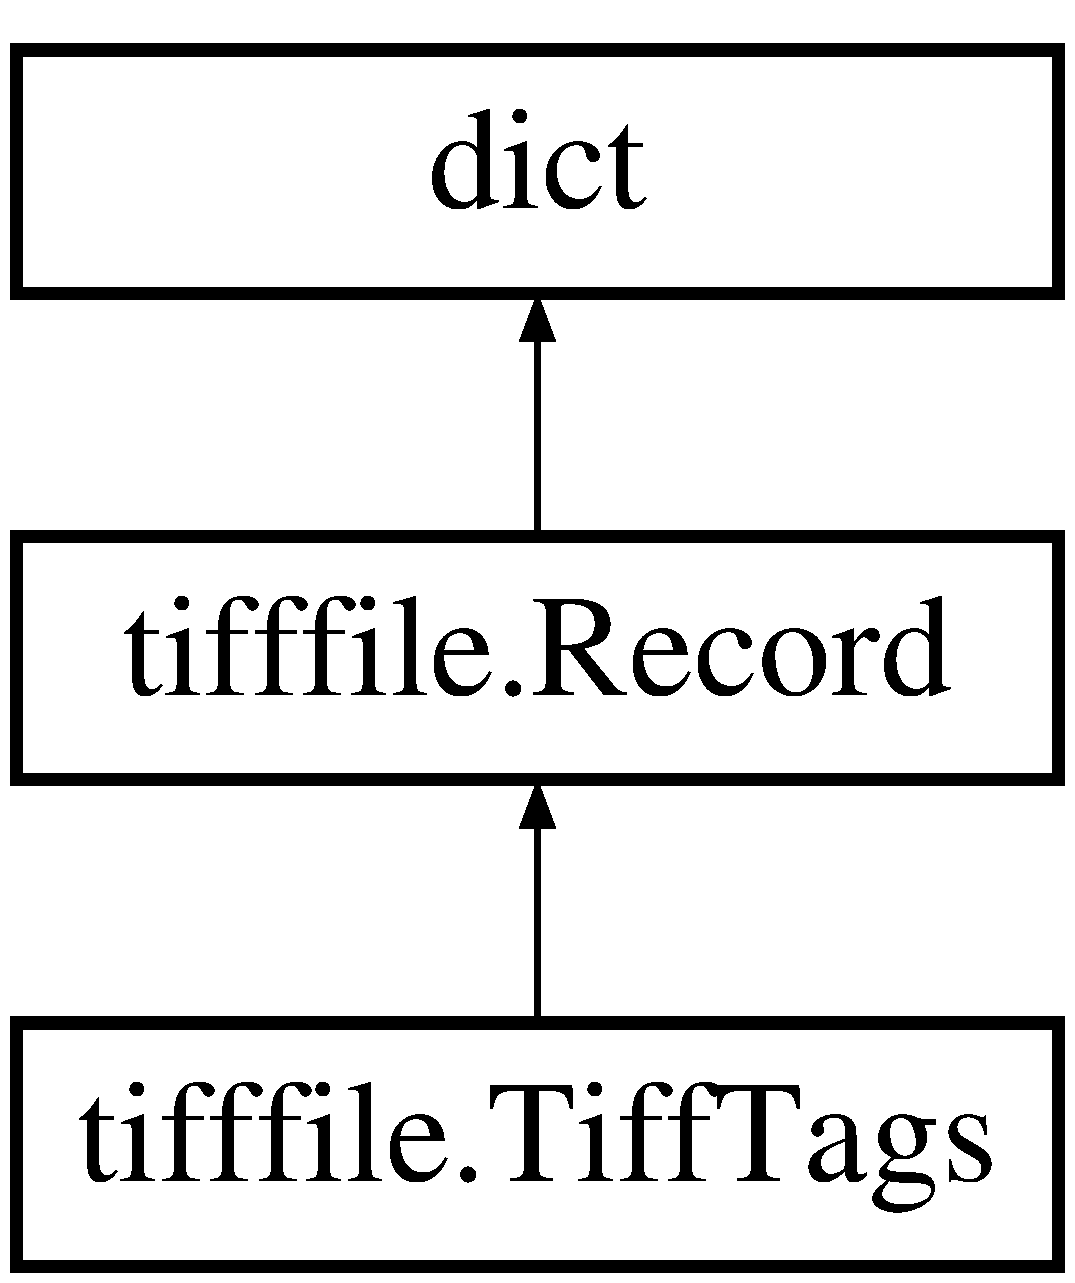
\includegraphics[height=3.000000cm]{classtifffile_1_1_record}
\end{center}
\end{figure}
\subsection*{Public Member Functions}
\begin{DoxyCompactItemize}
\item 
def \hyperlink{classtifffile_1_1_record_a0ff543c8d9ef139ba868177e0db7ac02}{\-\_\-\-\_\-init\-\_\-\-\_\-}
\item 
def \hyperlink{classtifffile_1_1_record_aeba3dd18a66ecb80f9d6fc09dae33a5d}{\-\_\-\-\_\-getattr\-\_\-\-\_\-}
\item 
def \hyperlink{classtifffile_1_1_record_a2fc93e114d60c64619cd6ea297c186bf}{\-\_\-\-\_\-setattr\-\_\-\-\_\-}
\item 
def \hyperlink{classtifffile_1_1_record_a6462a5901c01bd8644032e4c55005e57}{\-\_\-\-\_\-str\-\_\-\-\_\-}
\end{DoxyCompactItemize}


\subsection{Detailed Description}
\begin{DoxyVerb}Dictionary with attribute access.

Can also be initialized with numpy.core.records.record.\end{DoxyVerb}
 

\subsection{Constructor \& Destructor Documentation}
\hypertarget{classtifffile_1_1_record_a0ff543c8d9ef139ba868177e0db7ac02}{\index{tifffile\-::\-Record@{tifffile\-::\-Record}!\-\_\-\-\_\-init\-\_\-\-\_\-@{\-\_\-\-\_\-init\-\_\-\-\_\-}}
\index{\-\_\-\-\_\-init\-\_\-\-\_\-@{\-\_\-\-\_\-init\-\_\-\-\_\-}!tifffile::Record@{tifffile\-::\-Record}}
\subsubsection[{\-\_\-\-\_\-init\-\_\-\-\_\-}]{\setlength{\rightskip}{0pt plus 5cm}def tifffile.\-Record.\-\_\-\-\_\-init\-\_\-\-\_\- (
\begin{DoxyParamCaption}
\item[{}]{self, }
\item[{}]{arg = {\ttfamily None}, }
\item[{}]{kwargs}
\end{DoxyParamCaption}
)}}\label{classtifffile_1_1_record_a0ff543c8d9ef139ba868177e0db7ac02}


\subsection{Member Function Documentation}
\hypertarget{classtifffile_1_1_record_aeba3dd18a66ecb80f9d6fc09dae33a5d}{\index{tifffile\-::\-Record@{tifffile\-::\-Record}!\-\_\-\-\_\-getattr\-\_\-\-\_\-@{\-\_\-\-\_\-getattr\-\_\-\-\_\-}}
\index{\-\_\-\-\_\-getattr\-\_\-\-\_\-@{\-\_\-\-\_\-getattr\-\_\-\-\_\-}!tifffile::Record@{tifffile\-::\-Record}}
\subsubsection[{\-\_\-\-\_\-getattr\-\_\-\-\_\-}]{\setlength{\rightskip}{0pt plus 5cm}def tifffile.\-Record.\-\_\-\-\_\-getattr\-\_\-\-\_\- (
\begin{DoxyParamCaption}
\item[{}]{self, }
\item[{}]{name}
\end{DoxyParamCaption}
)}}\label{classtifffile_1_1_record_aeba3dd18a66ecb80f9d6fc09dae33a5d}
\hypertarget{classtifffile_1_1_record_a2fc93e114d60c64619cd6ea297c186bf}{\index{tifffile\-::\-Record@{tifffile\-::\-Record}!\-\_\-\-\_\-setattr\-\_\-\-\_\-@{\-\_\-\-\_\-setattr\-\_\-\-\_\-}}
\index{\-\_\-\-\_\-setattr\-\_\-\-\_\-@{\-\_\-\-\_\-setattr\-\_\-\-\_\-}!tifffile::Record@{tifffile\-::\-Record}}
\subsubsection[{\-\_\-\-\_\-setattr\-\_\-\-\_\-}]{\setlength{\rightskip}{0pt plus 5cm}def tifffile.\-Record.\-\_\-\-\_\-setattr\-\_\-\-\_\- (
\begin{DoxyParamCaption}
\item[{}]{self, }
\item[{}]{name, }
\item[{}]{value}
\end{DoxyParamCaption}
)}}\label{classtifffile_1_1_record_a2fc93e114d60c64619cd6ea297c186bf}
\hypertarget{classtifffile_1_1_record_a6462a5901c01bd8644032e4c55005e57}{\index{tifffile\-::\-Record@{tifffile\-::\-Record}!\-\_\-\-\_\-str\-\_\-\-\_\-@{\-\_\-\-\_\-str\-\_\-\-\_\-}}
\index{\-\_\-\-\_\-str\-\_\-\-\_\-@{\-\_\-\-\_\-str\-\_\-\-\_\-}!tifffile::Record@{tifffile\-::\-Record}}
\subsubsection[{\-\_\-\-\_\-str\-\_\-\-\_\-}]{\setlength{\rightskip}{0pt plus 5cm}def tifffile.\-Record.\-\_\-\-\_\-str\-\_\-\-\_\- (
\begin{DoxyParamCaption}
\item[{}]{self}
\end{DoxyParamCaption}
)}}\label{classtifffile_1_1_record_a6462a5901c01bd8644032e4c55005e57}
\begin{DoxyVerb}Pretty print Record.\end{DoxyVerb}
 

The documentation for this class was generated from the following file\-:\begin{DoxyCompactItemize}
\item 
workdir/atrex/\-Software/\hyperlink{tifffile_8py}{tifffile.\-py}\end{DoxyCompactItemize}

\hypertarget{class_j_c_p_d_s_1_1_reflection}{\section{J\-C\-P\-D\-S.\-Reflection Class Reference}
\label{class_j_c_p_d_s_1_1_reflection}\index{J\-C\-P\-D\-S.\-Reflection@{J\-C\-P\-D\-S.\-Reflection}}
}
\subsection*{Public Member Functions}
\begin{DoxyCompactItemize}
\item 
def \hyperlink{class_j_c_p_d_s_1_1_reflection_a60f239e7b0dc01ae22859aab4ce15958}{parse\-Vals}
\item 
def \hyperlink{class_j_c_p_d_s_1_1_reflection_a5b0c369390f0f6c9d4f43f79451666ad}{parse\-Vals\-X\-P\-O\-W}
\end{DoxyCompactItemize}
\subsection*{Public Attributes}
\begin{DoxyCompactItemize}
\item 
\hyperlink{class_j_c_p_d_s_1_1_reflection_a2e19b84f40e3e5dadbe49a60cd45406e}{d0}
\item 
\hyperlink{class_j_c_p_d_s_1_1_reflection_af4298638f38bd63f0731ee0d564f390d}{inten}
\item 
\hyperlink{class_j_c_p_d_s_1_1_reflection_aaab66547bee474122bb66caa9732b683}{h}
\item 
\hyperlink{class_j_c_p_d_s_1_1_reflection_a40102fb28adbda5bc337211845a3a3e3}{k}
\item 
\hyperlink{class_j_c_p_d_s_1_1_reflection_a678d14a1fe67331931242cc73ef096b9}{l}
\end{DoxyCompactItemize}
\subsection*{Static Public Attributes}
\begin{DoxyCompactItemize}
\item 
int \hyperlink{class_j_c_p_d_s_1_1_reflection_a21cdd847ccc4a67939ba0f7eddb288b5}{d0} = 0
\item 
int \hyperlink{class_j_c_p_d_s_1_1_reflection_a343546653e0fa7aa59c9ef63366d6d95}{d} = 0
\item 
int \hyperlink{class_j_c_p_d_s_1_1_reflection_a0122c97dba87bbee7195978f098a6e77}{inten} = 0
\item 
int \hyperlink{class_j_c_p_d_s_1_1_reflection_a9e23ae17c46a767f5b54e8c3f03e48f2}{h} = 0
\item 
int \hyperlink{class_j_c_p_d_s_1_1_reflection_acf1308b53630e8382c97b0d9ebb25bf3}{k} = 0
\item 
int \hyperlink{class_j_c_p_d_s_1_1_reflection_af56bfe0782709d77e267c57b198c3e0a}{l} = 0
\end{DoxyCompactItemize}


\subsection{Member Function Documentation}
\hypertarget{class_j_c_p_d_s_1_1_reflection_a60f239e7b0dc01ae22859aab4ce15958}{\index{J\-C\-P\-D\-S\-::\-Reflection@{J\-C\-P\-D\-S\-::\-Reflection}!parse\-Vals@{parse\-Vals}}
\index{parse\-Vals@{parse\-Vals}!JCPDS::Reflection@{J\-C\-P\-D\-S\-::\-Reflection}}
\subsubsection[{parse\-Vals}]{\setlength{\rightskip}{0pt plus 5cm}def J\-C\-P\-D\-S.\-Reflection.\-parse\-Vals (
\begin{DoxyParamCaption}
\item[{}]{self, }
\item[{}]{instr}
\end{DoxyParamCaption}
)}}\label{class_j_c_p_d_s_1_1_reflection_a60f239e7b0dc01ae22859aab4ce15958}
\hypertarget{class_j_c_p_d_s_1_1_reflection_a5b0c369390f0f6c9d4f43f79451666ad}{\index{J\-C\-P\-D\-S\-::\-Reflection@{J\-C\-P\-D\-S\-::\-Reflection}!parse\-Vals\-X\-P\-O\-W@{parse\-Vals\-X\-P\-O\-W}}
\index{parse\-Vals\-X\-P\-O\-W@{parse\-Vals\-X\-P\-O\-W}!JCPDS::Reflection@{J\-C\-P\-D\-S\-::\-Reflection}}
\subsubsection[{parse\-Vals\-X\-P\-O\-W}]{\setlength{\rightskip}{0pt plus 5cm}def J\-C\-P\-D\-S.\-Reflection.\-parse\-Vals\-X\-P\-O\-W (
\begin{DoxyParamCaption}
\item[{}]{self, }
\item[{}]{instr}
\end{DoxyParamCaption}
)}}\label{class_j_c_p_d_s_1_1_reflection_a5b0c369390f0f6c9d4f43f79451666ad}


\subsection{Member Data Documentation}
\hypertarget{class_j_c_p_d_s_1_1_reflection_a343546653e0fa7aa59c9ef63366d6d95}{\index{J\-C\-P\-D\-S\-::\-Reflection@{J\-C\-P\-D\-S\-::\-Reflection}!d@{d}}
\index{d@{d}!JCPDS::Reflection@{J\-C\-P\-D\-S\-::\-Reflection}}
\subsubsection[{d}]{\setlength{\rightskip}{0pt plus 5cm}int J\-C\-P\-D\-S.\-Reflection.\-d = 0\hspace{0.3cm}{\ttfamily [static]}}}\label{class_j_c_p_d_s_1_1_reflection_a343546653e0fa7aa59c9ef63366d6d95}
\hypertarget{class_j_c_p_d_s_1_1_reflection_a21cdd847ccc4a67939ba0f7eddb288b5}{\index{J\-C\-P\-D\-S\-::\-Reflection@{J\-C\-P\-D\-S\-::\-Reflection}!d0@{d0}}
\index{d0@{d0}!JCPDS::Reflection@{J\-C\-P\-D\-S\-::\-Reflection}}
\subsubsection[{d0}]{\setlength{\rightskip}{0pt plus 5cm}int J\-C\-P\-D\-S.\-Reflection.\-d0 = 0\hspace{0.3cm}{\ttfamily [static]}}}\label{class_j_c_p_d_s_1_1_reflection_a21cdd847ccc4a67939ba0f7eddb288b5}
\hypertarget{class_j_c_p_d_s_1_1_reflection_a2e19b84f40e3e5dadbe49a60cd45406e}{\index{J\-C\-P\-D\-S\-::\-Reflection@{J\-C\-P\-D\-S\-::\-Reflection}!d0@{d0}}
\index{d0@{d0}!JCPDS::Reflection@{J\-C\-P\-D\-S\-::\-Reflection}}
\subsubsection[{d0}]{\setlength{\rightskip}{0pt plus 5cm}J\-C\-P\-D\-S.\-Reflection.\-d0}}\label{class_j_c_p_d_s_1_1_reflection_a2e19b84f40e3e5dadbe49a60cd45406e}
\hypertarget{class_j_c_p_d_s_1_1_reflection_a9e23ae17c46a767f5b54e8c3f03e48f2}{\index{J\-C\-P\-D\-S\-::\-Reflection@{J\-C\-P\-D\-S\-::\-Reflection}!h@{h}}
\index{h@{h}!JCPDS::Reflection@{J\-C\-P\-D\-S\-::\-Reflection}}
\subsubsection[{h}]{\setlength{\rightskip}{0pt plus 5cm}int J\-C\-P\-D\-S.\-Reflection.\-h = 0\hspace{0.3cm}{\ttfamily [static]}}}\label{class_j_c_p_d_s_1_1_reflection_a9e23ae17c46a767f5b54e8c3f03e48f2}
\hypertarget{class_j_c_p_d_s_1_1_reflection_aaab66547bee474122bb66caa9732b683}{\index{J\-C\-P\-D\-S\-::\-Reflection@{J\-C\-P\-D\-S\-::\-Reflection}!h@{h}}
\index{h@{h}!JCPDS::Reflection@{J\-C\-P\-D\-S\-::\-Reflection}}
\subsubsection[{h}]{\setlength{\rightskip}{0pt plus 5cm}J\-C\-P\-D\-S.\-Reflection.\-h}}\label{class_j_c_p_d_s_1_1_reflection_aaab66547bee474122bb66caa9732b683}
\hypertarget{class_j_c_p_d_s_1_1_reflection_a0122c97dba87bbee7195978f098a6e77}{\index{J\-C\-P\-D\-S\-::\-Reflection@{J\-C\-P\-D\-S\-::\-Reflection}!inten@{inten}}
\index{inten@{inten}!JCPDS::Reflection@{J\-C\-P\-D\-S\-::\-Reflection}}
\subsubsection[{inten}]{\setlength{\rightskip}{0pt plus 5cm}int J\-C\-P\-D\-S.\-Reflection.\-inten = 0\hspace{0.3cm}{\ttfamily [static]}}}\label{class_j_c_p_d_s_1_1_reflection_a0122c97dba87bbee7195978f098a6e77}
\hypertarget{class_j_c_p_d_s_1_1_reflection_af4298638f38bd63f0731ee0d564f390d}{\index{J\-C\-P\-D\-S\-::\-Reflection@{J\-C\-P\-D\-S\-::\-Reflection}!inten@{inten}}
\index{inten@{inten}!JCPDS::Reflection@{J\-C\-P\-D\-S\-::\-Reflection}}
\subsubsection[{inten}]{\setlength{\rightskip}{0pt plus 5cm}J\-C\-P\-D\-S.\-Reflection.\-inten}}\label{class_j_c_p_d_s_1_1_reflection_af4298638f38bd63f0731ee0d564f390d}
\hypertarget{class_j_c_p_d_s_1_1_reflection_acf1308b53630e8382c97b0d9ebb25bf3}{\index{J\-C\-P\-D\-S\-::\-Reflection@{J\-C\-P\-D\-S\-::\-Reflection}!k@{k}}
\index{k@{k}!JCPDS::Reflection@{J\-C\-P\-D\-S\-::\-Reflection}}
\subsubsection[{k}]{\setlength{\rightskip}{0pt plus 5cm}int J\-C\-P\-D\-S.\-Reflection.\-k = 0\hspace{0.3cm}{\ttfamily [static]}}}\label{class_j_c_p_d_s_1_1_reflection_acf1308b53630e8382c97b0d9ebb25bf3}
\hypertarget{class_j_c_p_d_s_1_1_reflection_a40102fb28adbda5bc337211845a3a3e3}{\index{J\-C\-P\-D\-S\-::\-Reflection@{J\-C\-P\-D\-S\-::\-Reflection}!k@{k}}
\index{k@{k}!JCPDS::Reflection@{J\-C\-P\-D\-S\-::\-Reflection}}
\subsubsection[{k}]{\setlength{\rightskip}{0pt plus 5cm}J\-C\-P\-D\-S.\-Reflection.\-k}}\label{class_j_c_p_d_s_1_1_reflection_a40102fb28adbda5bc337211845a3a3e3}
\hypertarget{class_j_c_p_d_s_1_1_reflection_af56bfe0782709d77e267c57b198c3e0a}{\index{J\-C\-P\-D\-S\-::\-Reflection@{J\-C\-P\-D\-S\-::\-Reflection}!l@{l}}
\index{l@{l}!JCPDS::Reflection@{J\-C\-P\-D\-S\-::\-Reflection}}
\subsubsection[{l}]{\setlength{\rightskip}{0pt plus 5cm}int J\-C\-P\-D\-S.\-Reflection.\-l = 0\hspace{0.3cm}{\ttfamily [static]}}}\label{class_j_c_p_d_s_1_1_reflection_af56bfe0782709d77e267c57b198c3e0a}
\hypertarget{class_j_c_p_d_s_1_1_reflection_a678d14a1fe67331931242cc73ef096b9}{\index{J\-C\-P\-D\-S\-::\-Reflection@{J\-C\-P\-D\-S\-::\-Reflection}!l@{l}}
\index{l@{l}!JCPDS::Reflection@{J\-C\-P\-D\-S\-::\-Reflection}}
\subsubsection[{l}]{\setlength{\rightskip}{0pt plus 5cm}J\-C\-P\-D\-S.\-Reflection.\-l}}\label{class_j_c_p_d_s_1_1_reflection_a678d14a1fe67331931242cc73ef096b9}


The documentation for this class was generated from the following file\-:\begin{DoxyCompactItemize}
\item 
workdir/atrex/\-Software/\hyperlink{_j_c_p_d_s_8py}{J\-C\-P\-D\-S.\-py}\end{DoxyCompactItemize}

\hypertarget{classsimulate_dlg_1_1simulate_dlg}{\section{simulate\-Dlg.\-simulate\-Dlg Class Reference}
\label{classsimulate_dlg_1_1simulate_dlg}\index{simulate\-Dlg.\-simulate\-Dlg@{simulate\-Dlg.\-simulate\-Dlg}}
}
Inheritance diagram for simulate\-Dlg.\-simulate\-Dlg\-:\begin{figure}[H]
\begin{center}
\leavevmode
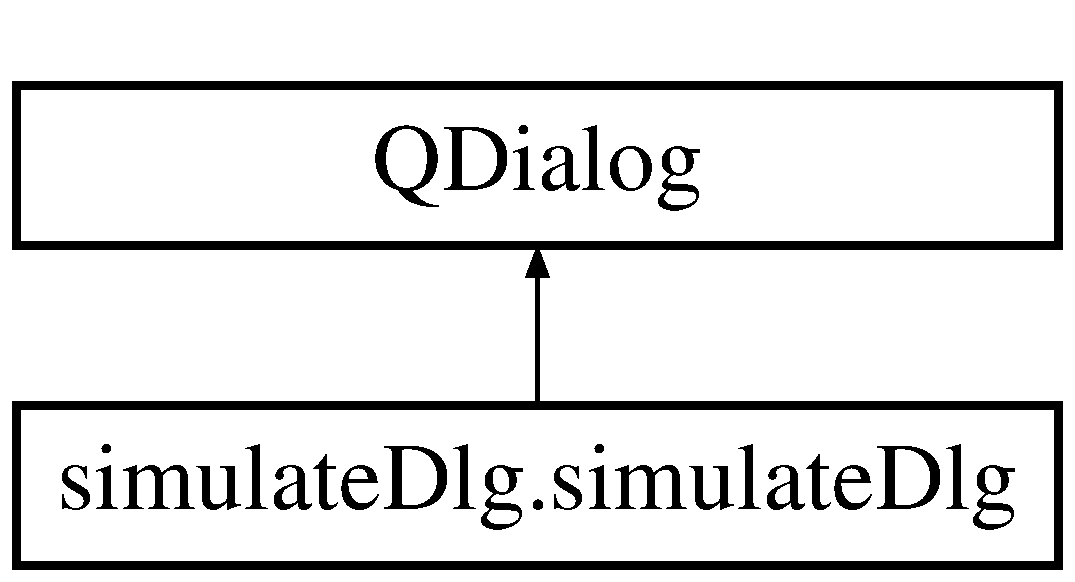
\includegraphics[height=2.000000cm]{classsimulate_dlg_1_1simulate_dlg}
\end{center}
\end{figure}
\subsection*{Public Member Functions}
\begin{DoxyCompactItemize}
\item 
def \hyperlink{classsimulate_dlg_1_1simulate_dlg_a30e20ab290a85ace9b9f1aa244d7c474}{\-\_\-\-\_\-init\-\_\-\-\_\-}
\item 
def \hyperlink{classsimulate_dlg_1_1simulate_dlg_ae8ad62465bea76aeb7ced4d34d8ca56a}{set\-Work\-Dir}
\item 
def \hyperlink{classsimulate_dlg_1_1simulate_dlg_a53b3c5047a7a281b5baeec7135492591}{set\-B\-Size\-Control}
\item 
def \hyperlink{classsimulate_dlg_1_1simulate_dlg_a97123c1f3e8b1b340dc382a6fd86a101}{set\-Exclude\-Control}
\item 
def \hyperlink{classsimulate_dlg_1_1simulate_dlg_abe6b4f3fef4b78d2c7a2555727653de1}{set\-Detector}
\item 
def \hyperlink{classsimulate_dlg_1_1simulate_dlg_a3087ff8625ca2596757a04e8d57c6aef}{set\-Peak\-Table}
\item 
def \hyperlink{classsimulate_dlg_1_1simulate_dlg_ac656f0af5fb6ead3d58c3a79cbe90453}{set\-Predict}
\item 
def \hyperlink{classsimulate_dlg_1_1simulate_dlg_afc7435e2812554e7059d3d9e908183ff}{set\-Project}
\item 
def \hyperlink{classsimulate_dlg_1_1simulate_dlg_a251194e1c458621e24fdfdeb409342c6}{fill\-Up}
\item 
def \hyperlink{classsimulate_dlg_1_1simulate_dlg_a8d07b8b8fbaebf05066a368ef55d1c3e}{inc\-Val}
\item 
def \hyperlink{classsimulate_dlg_1_1simulate_dlg_a686a9c2d3206667c4f54f742537dc0f4}{dec\-Val}
\item 
def \hyperlink{classsimulate_dlg_1_1simulate_dlg_ae7f76a72f48eadc2aa799a2a2a66c24f}{rad\-State}
\item 
def \hyperlink{classsimulate_dlg_1_1simulate_dlg_a9c525e6091e98de8f7da2fa5390e7f45}{gen\-B}
\item 
def \hyperlink{classsimulate_dlg_1_1simulate_dlg_a5420da8b718295dec6996e3af575d009}{change\-B}
\item 
def \hyperlink{classsimulate_dlg_1_1simulate_dlg_ab5bf1b8be44923ad6767d7b26e24dfba}{reset\-O\-C\-P}
\item 
def \hyperlink{classsimulate_dlg_1_1simulate_dlg_a36b13c633095fd1b37a8c24bdc9feb02}{read\-\_\-\-L\-P}
\item 
def \hyperlink{classsimulate_dlg_1_1simulate_dlg_a541dcb68081dc45190cf99d019e34abb}{print\-\_\-\-L\-P}
\item 
def \hyperlink{classsimulate_dlg_1_1simulate_dlg_a670a1ff9f543741845ce493b6cd74a3c}{open\-U\-B}
\begin{DoxyCompactList}\small\item\em open U\-B matrix \end{DoxyCompactList}\item 
def \hyperlink{classsimulate_dlg_1_1simulate_dlg_a581c5c28fe9bf57a0de93fcb1e8859aa}{load\-U\-B}
\item 
def \hyperlink{classsimulate_dlg_1_1simulate_dlg_af4dec6ad7208da45bb52d9d42f4d16ce}{save\-U\-B}
\item 
def \hyperlink{classsimulate_dlg_1_1simulate_dlg_ad9f8e5700a177c99d6d602a897240408}{display\-Matrix}
\item 
def \hyperlink{classsimulate_dlg_1_1simulate_dlg_aa4af2d01c58f4243d379c31a9a46f45c}{assign\-H\-K\-L}
\item 
def \hyperlink{classsimulate_dlg_1_1simulate_dlg_a234c4ec7bdd66c1146e769d3e2cb757b}{generate}
\item 
def \hyperlink{classsimulate_dlg_1_1simulate_dlg_a1e8f99f0c2ba8218f61c039d7456a62a}{index}
\item 
def \hyperlink{classsimulate_dlg_1_1simulate_dlg_a5785ed6c6f50cc4276949b204b39dd62}{get\-Bravais\-Type}
\item 
def \hyperlink{classsimulate_dlg_1_1simulate_dlg_a6bc9d5aedaf9bf4452cb118b7a4dab01}{generate\-\_\-laue}
\item 
def \hyperlink{classsimulate_dlg_1_1simulate_dlg_ad93d6457999611add68e57fea7270e2a}{generate\-\_\-mono}
\item 
def \hyperlink{classsimulate_dlg_1_1simulate_dlg_a2c6753d7216124538a12c8b5f8157c43}{read\-\_\-box\-\_\-size}
\item 
def \hyperlink{classsimulate_dlg_1_1simulate_dlg_a3464acfdc69fd672f3ea82d6408fede7}{close\-Up}
\end{DoxyCompactItemize}
\subsection*{Public Attributes}
\begin{DoxyCompactItemize}
\item 
\hyperlink{classsimulate_dlg_1_1simulate_dlg_a23a3d39d70f0ae6ce8a838fe680afd08}{ui}
\item 
\hyperlink{classsimulate_dlg_1_1simulate_dlg_ad2226009f457b82889ed337b1ed49e4b}{my\-Detect}
\item 
\hyperlink{classsimulate_dlg_1_1simulate_dlg_a5aa51d22e30acd26145131e848e30759}{ub}
\item 
\hyperlink{classsimulate_dlg_1_1simulate_dlg_afb873a7d23504a37dc242405343f64aa}{my\-Predict}
\item 
\hyperlink{classsimulate_dlg_1_1simulate_dlg_a714be7d1a5fb648271c987444d5be3c4}{my\-Peaks}
\item 
\hyperlink{classsimulate_dlg_1_1simulate_dlg_aed2a79b17c8c625b06bad686996395e8}{brav\-Type}
\item 
\hyperlink{classsimulate_dlg_1_1simulate_dlg_a217be5c43518b4f44ac9f9397e4cd155}{workdir}
\item 
\hyperlink{classsimulate_dlg_1_1simulate_dlg_a37752b91546a36f94ff8e4dedee83518}{base}
\item 
\hyperlink{classsimulate_dlg_1_1simulate_dlg_a6b8afedfdaab0461117c61cde727aa2d}{proj\-Flag}
\item 
\hyperlink{classsimulate_dlg_1_1simulate_dlg_a2b03e2e70fbf25c638c1e0466a2de38f}{bs\-Control}
\item 
\hyperlink{classsimulate_dlg_1_1simulate_dlg_a2adb9273893575b3120e8878a99983d4}{exclude\-C\-Box}
\item 
\hyperlink{classsimulate_dlg_1_1simulate_dlg_a723b0e1c3aa3f071ae84ec39a1558845}{project}
\end{DoxyCompactItemize}
\subsection*{Static Public Attributes}
\begin{DoxyCompactItemize}
\item 
tuple \hyperlink{classsimulate_dlg_1_1simulate_dlg_a14c3146ee7422f53d8488a114344800e}{update\-Peaks} = Qt\-Core.\-pyqt\-Signal()
\item 
tuple \hyperlink{classsimulate_dlg_1_1simulate_dlg_a1c6d77c7b4759cb95a7fbdd5a7ca23d7}{update\-Display} = Qt\-Core.\-pyqt\-Signal()
\end{DoxyCompactItemize}


\subsection{Constructor \& Destructor Documentation}
\hypertarget{classsimulate_dlg_1_1simulate_dlg_a30e20ab290a85ace9b9f1aa244d7c474}{\index{simulate\-Dlg\-::simulate\-Dlg@{simulate\-Dlg\-::simulate\-Dlg}!\-\_\-\-\_\-init\-\_\-\-\_\-@{\-\_\-\-\_\-init\-\_\-\-\_\-}}
\index{\-\_\-\-\_\-init\-\_\-\-\_\-@{\-\_\-\-\_\-init\-\_\-\-\_\-}!simulateDlg::simulateDlg@{simulate\-Dlg\-::simulate\-Dlg}}
\subsubsection[{\-\_\-\-\_\-init\-\_\-\-\_\-}]{\setlength{\rightskip}{0pt plus 5cm}def simulate\-Dlg.\-simulate\-Dlg.\-\_\-\-\_\-init\-\_\-\-\_\- (
\begin{DoxyParamCaption}
\item[{}]{self}
\end{DoxyParamCaption}
)}}\label{classsimulate_dlg_1_1simulate_dlg_a30e20ab290a85ace9b9f1aa244d7c474}


\subsection{Member Function Documentation}
\hypertarget{classsimulate_dlg_1_1simulate_dlg_aa4af2d01c58f4243d379c31a9a46f45c}{\index{simulate\-Dlg\-::simulate\-Dlg@{simulate\-Dlg\-::simulate\-Dlg}!assign\-H\-K\-L@{assign\-H\-K\-L}}
\index{assign\-H\-K\-L@{assign\-H\-K\-L}!simulateDlg::simulateDlg@{simulate\-Dlg\-::simulate\-Dlg}}
\subsubsection[{assign\-H\-K\-L}]{\setlength{\rightskip}{0pt plus 5cm}def simulate\-Dlg.\-simulate\-Dlg.\-assign\-H\-K\-L (
\begin{DoxyParamCaption}
\item[{}]{self}
\end{DoxyParamCaption}
)}}\label{classsimulate_dlg_1_1simulate_dlg_aa4af2d01c58f4243d379c31a9a46f45c}
\hypertarget{classsimulate_dlg_1_1simulate_dlg_a5420da8b718295dec6996e3af575d009}{\index{simulate\-Dlg\-::simulate\-Dlg@{simulate\-Dlg\-::simulate\-Dlg}!change\-B@{change\-B}}
\index{change\-B@{change\-B}!simulateDlg::simulateDlg@{simulate\-Dlg\-::simulate\-Dlg}}
\subsubsection[{change\-B}]{\setlength{\rightskip}{0pt plus 5cm}def simulate\-Dlg.\-simulate\-Dlg.\-change\-B (
\begin{DoxyParamCaption}
\item[{}]{self}
\end{DoxyParamCaption}
)}}\label{classsimulate_dlg_1_1simulate_dlg_a5420da8b718295dec6996e3af575d009}
\hypertarget{classsimulate_dlg_1_1simulate_dlg_a3464acfdc69fd672f3ea82d6408fede7}{\index{simulate\-Dlg\-::simulate\-Dlg@{simulate\-Dlg\-::simulate\-Dlg}!close\-Up@{close\-Up}}
\index{close\-Up@{close\-Up}!simulateDlg::simulateDlg@{simulate\-Dlg\-::simulate\-Dlg}}
\subsubsection[{close\-Up}]{\setlength{\rightskip}{0pt plus 5cm}def simulate\-Dlg.\-simulate\-Dlg.\-close\-Up (
\begin{DoxyParamCaption}
\item[{}]{self}
\end{DoxyParamCaption}
)}}\label{classsimulate_dlg_1_1simulate_dlg_a3464acfdc69fd672f3ea82d6408fede7}
\hypertarget{classsimulate_dlg_1_1simulate_dlg_a686a9c2d3206667c4f54f742537dc0f4}{\index{simulate\-Dlg\-::simulate\-Dlg@{simulate\-Dlg\-::simulate\-Dlg}!dec\-Val@{dec\-Val}}
\index{dec\-Val@{dec\-Val}!simulateDlg::simulateDlg@{simulate\-Dlg\-::simulate\-Dlg}}
\subsubsection[{dec\-Val}]{\setlength{\rightskip}{0pt plus 5cm}def simulate\-Dlg.\-simulate\-Dlg.\-dec\-Val (
\begin{DoxyParamCaption}
\item[{}]{self}
\end{DoxyParamCaption}
)}}\label{classsimulate_dlg_1_1simulate_dlg_a686a9c2d3206667c4f54f742537dc0f4}
\hypertarget{classsimulate_dlg_1_1simulate_dlg_ad9f8e5700a177c99d6d602a897240408}{\index{simulate\-Dlg\-::simulate\-Dlg@{simulate\-Dlg\-::simulate\-Dlg}!display\-Matrix@{display\-Matrix}}
\index{display\-Matrix@{display\-Matrix}!simulateDlg::simulateDlg@{simulate\-Dlg\-::simulate\-Dlg}}
\subsubsection[{display\-Matrix}]{\setlength{\rightskip}{0pt plus 5cm}def simulate\-Dlg.\-simulate\-Dlg.\-display\-Matrix (
\begin{DoxyParamCaption}
\item[{}]{self, }
\item[{}]{mat\-Type}
\end{DoxyParamCaption}
)}}\label{classsimulate_dlg_1_1simulate_dlg_ad9f8e5700a177c99d6d602a897240408}
\hypertarget{classsimulate_dlg_1_1simulate_dlg_a251194e1c458621e24fdfdeb409342c6}{\index{simulate\-Dlg\-::simulate\-Dlg@{simulate\-Dlg\-::simulate\-Dlg}!fill\-Up@{fill\-Up}}
\index{fill\-Up@{fill\-Up}!simulateDlg::simulateDlg@{simulate\-Dlg\-::simulate\-Dlg}}
\subsubsection[{fill\-Up}]{\setlength{\rightskip}{0pt plus 5cm}def simulate\-Dlg.\-simulate\-Dlg.\-fill\-Up (
\begin{DoxyParamCaption}
\item[{}]{self}
\end{DoxyParamCaption}
)}}\label{classsimulate_dlg_1_1simulate_dlg_a251194e1c458621e24fdfdeb409342c6}
\hypertarget{classsimulate_dlg_1_1simulate_dlg_a9c525e6091e98de8f7da2fa5390e7f45}{\index{simulate\-Dlg\-::simulate\-Dlg@{simulate\-Dlg\-::simulate\-Dlg}!gen\-B@{gen\-B}}
\index{gen\-B@{gen\-B}!simulateDlg::simulateDlg@{simulate\-Dlg\-::simulate\-Dlg}}
\subsubsection[{gen\-B}]{\setlength{\rightskip}{0pt plus 5cm}def simulate\-Dlg.\-simulate\-Dlg.\-gen\-B (
\begin{DoxyParamCaption}
\item[{}]{self}
\end{DoxyParamCaption}
)}}\label{classsimulate_dlg_1_1simulate_dlg_a9c525e6091e98de8f7da2fa5390e7f45}
\hypertarget{classsimulate_dlg_1_1simulate_dlg_a234c4ec7bdd66c1146e769d3e2cb757b}{\index{simulate\-Dlg\-::simulate\-Dlg@{simulate\-Dlg\-::simulate\-Dlg}!generate@{generate}}
\index{generate@{generate}!simulateDlg::simulateDlg@{simulate\-Dlg\-::simulate\-Dlg}}
\subsubsection[{generate}]{\setlength{\rightskip}{0pt plus 5cm}def simulate\-Dlg.\-simulate\-Dlg.\-generate (
\begin{DoxyParamCaption}
\item[{}]{self}
\end{DoxyParamCaption}
)}}\label{classsimulate_dlg_1_1simulate_dlg_a234c4ec7bdd66c1146e769d3e2cb757b}
\hypertarget{classsimulate_dlg_1_1simulate_dlg_a6bc9d5aedaf9bf4452cb118b7a4dab01}{\index{simulate\-Dlg\-::simulate\-Dlg@{simulate\-Dlg\-::simulate\-Dlg}!generate\-\_\-laue@{generate\-\_\-laue}}
\index{generate\-\_\-laue@{generate\-\_\-laue}!simulateDlg::simulateDlg@{simulate\-Dlg\-::simulate\-Dlg}}
\subsubsection[{generate\-\_\-laue}]{\setlength{\rightskip}{0pt plus 5cm}def simulate\-Dlg.\-simulate\-Dlg.\-generate\-\_\-laue (
\begin{DoxyParamCaption}
\item[{}]{self}
\end{DoxyParamCaption}
)}}\label{classsimulate_dlg_1_1simulate_dlg_a6bc9d5aedaf9bf4452cb118b7a4dab01}
\hypertarget{classsimulate_dlg_1_1simulate_dlg_ad93d6457999611add68e57fea7270e2a}{\index{simulate\-Dlg\-::simulate\-Dlg@{simulate\-Dlg\-::simulate\-Dlg}!generate\-\_\-mono@{generate\-\_\-mono}}
\index{generate\-\_\-mono@{generate\-\_\-mono}!simulateDlg::simulateDlg@{simulate\-Dlg\-::simulate\-Dlg}}
\subsubsection[{generate\-\_\-mono}]{\setlength{\rightskip}{0pt plus 5cm}def simulate\-Dlg.\-simulate\-Dlg.\-generate\-\_\-mono (
\begin{DoxyParamCaption}
\item[{}]{self}
\end{DoxyParamCaption}
)}}\label{classsimulate_dlg_1_1simulate_dlg_ad93d6457999611add68e57fea7270e2a}
\hypertarget{classsimulate_dlg_1_1simulate_dlg_a5785ed6c6f50cc4276949b204b39dd62}{\index{simulate\-Dlg\-::simulate\-Dlg@{simulate\-Dlg\-::simulate\-Dlg}!get\-Bravais\-Type@{get\-Bravais\-Type}}
\index{get\-Bravais\-Type@{get\-Bravais\-Type}!simulateDlg::simulateDlg@{simulate\-Dlg\-::simulate\-Dlg}}
\subsubsection[{get\-Bravais\-Type}]{\setlength{\rightskip}{0pt plus 5cm}def simulate\-Dlg.\-simulate\-Dlg.\-get\-Bravais\-Type (
\begin{DoxyParamCaption}
\item[{}]{self}
\end{DoxyParamCaption}
)}}\label{classsimulate_dlg_1_1simulate_dlg_a5785ed6c6f50cc4276949b204b39dd62}
\hypertarget{classsimulate_dlg_1_1simulate_dlg_a8d07b8b8fbaebf05066a368ef55d1c3e}{\index{simulate\-Dlg\-::simulate\-Dlg@{simulate\-Dlg\-::simulate\-Dlg}!inc\-Val@{inc\-Val}}
\index{inc\-Val@{inc\-Val}!simulateDlg::simulateDlg@{simulate\-Dlg\-::simulate\-Dlg}}
\subsubsection[{inc\-Val}]{\setlength{\rightskip}{0pt plus 5cm}def simulate\-Dlg.\-simulate\-Dlg.\-inc\-Val (
\begin{DoxyParamCaption}
\item[{}]{self}
\end{DoxyParamCaption}
)}}\label{classsimulate_dlg_1_1simulate_dlg_a8d07b8b8fbaebf05066a368ef55d1c3e}
\hypertarget{classsimulate_dlg_1_1simulate_dlg_a1e8f99f0c2ba8218f61c039d7456a62a}{\index{simulate\-Dlg\-::simulate\-Dlg@{simulate\-Dlg\-::simulate\-Dlg}!index@{index}}
\index{index@{index}!simulateDlg::simulateDlg@{simulate\-Dlg\-::simulate\-Dlg}}
\subsubsection[{index}]{\setlength{\rightskip}{0pt plus 5cm}def simulate\-Dlg.\-simulate\-Dlg.\-index (
\begin{DoxyParamCaption}
\item[{}]{self}
\end{DoxyParamCaption}
)}}\label{classsimulate_dlg_1_1simulate_dlg_a1e8f99f0c2ba8218f61c039d7456a62a}
\hypertarget{classsimulate_dlg_1_1simulate_dlg_a581c5c28fe9bf57a0de93fcb1e8859aa}{\index{simulate\-Dlg\-::simulate\-Dlg@{simulate\-Dlg\-::simulate\-Dlg}!load\-U\-B@{load\-U\-B}}
\index{load\-U\-B@{load\-U\-B}!simulateDlg::simulateDlg@{simulate\-Dlg\-::simulate\-Dlg}}
\subsubsection[{load\-U\-B}]{\setlength{\rightskip}{0pt plus 5cm}def simulate\-Dlg.\-simulate\-Dlg.\-load\-U\-B (
\begin{DoxyParamCaption}
\item[{}]{self, }
\item[{}]{fname}
\end{DoxyParamCaption}
)}}\label{classsimulate_dlg_1_1simulate_dlg_a581c5c28fe9bf57a0de93fcb1e8859aa}
\hypertarget{classsimulate_dlg_1_1simulate_dlg_a670a1ff9f543741845ce493b6cd74a3c}{\index{simulate\-Dlg\-::simulate\-Dlg@{simulate\-Dlg\-::simulate\-Dlg}!open\-U\-B@{open\-U\-B}}
\index{open\-U\-B@{open\-U\-B}!simulateDlg::simulateDlg@{simulate\-Dlg\-::simulate\-Dlg}}
\subsubsection[{open\-U\-B}]{\setlength{\rightskip}{0pt plus 5cm}def simulate\-Dlg.\-simulate\-Dlg.\-open\-U\-B (
\begin{DoxyParamCaption}
\item[{}]{self}
\end{DoxyParamCaption}
)}}\label{classsimulate_dlg_1_1simulate_dlg_a670a1ff9f543741845ce493b6cd74a3c}


open U\-B matrix 

\hypertarget{classsimulate_dlg_1_1simulate_dlg_a541dcb68081dc45190cf99d019e34abb}{\index{simulate\-Dlg\-::simulate\-Dlg@{simulate\-Dlg\-::simulate\-Dlg}!print\-\_\-\-L\-P@{print\-\_\-\-L\-P}}
\index{print\-\_\-\-L\-P@{print\-\_\-\-L\-P}!simulateDlg::simulateDlg@{simulate\-Dlg\-::simulate\-Dlg}}
\subsubsection[{print\-\_\-\-L\-P}]{\setlength{\rightskip}{0pt plus 5cm}def simulate\-Dlg.\-simulate\-Dlg.\-print\-\_\-\-L\-P (
\begin{DoxyParamCaption}
\item[{}]{self, }
\item[{}]{lp}
\end{DoxyParamCaption}
)}}\label{classsimulate_dlg_1_1simulate_dlg_a541dcb68081dc45190cf99d019e34abb}
\hypertarget{classsimulate_dlg_1_1simulate_dlg_ae7f76a72f48eadc2aa799a2a2a66c24f}{\index{simulate\-Dlg\-::simulate\-Dlg@{simulate\-Dlg\-::simulate\-Dlg}!rad\-State@{rad\-State}}
\index{rad\-State@{rad\-State}!simulateDlg::simulateDlg@{simulate\-Dlg\-::simulate\-Dlg}}
\subsubsection[{rad\-State}]{\setlength{\rightskip}{0pt plus 5cm}def simulate\-Dlg.\-simulate\-Dlg.\-rad\-State (
\begin{DoxyParamCaption}
\item[{}]{self}
\end{DoxyParamCaption}
)}}\label{classsimulate_dlg_1_1simulate_dlg_ae7f76a72f48eadc2aa799a2a2a66c24f}
\hypertarget{classsimulate_dlg_1_1simulate_dlg_a2c6753d7216124538a12c8b5f8157c43}{\index{simulate\-Dlg\-::simulate\-Dlg@{simulate\-Dlg\-::simulate\-Dlg}!read\-\_\-box\-\_\-size@{read\-\_\-box\-\_\-size}}
\index{read\-\_\-box\-\_\-size@{read\-\_\-box\-\_\-size}!simulateDlg::simulateDlg@{simulate\-Dlg\-::simulate\-Dlg}}
\subsubsection[{read\-\_\-box\-\_\-size}]{\setlength{\rightskip}{0pt plus 5cm}def simulate\-Dlg.\-simulate\-Dlg.\-read\-\_\-box\-\_\-size (
\begin{DoxyParamCaption}
\item[{}]{self}
\end{DoxyParamCaption}
)}}\label{classsimulate_dlg_1_1simulate_dlg_a2c6753d7216124538a12c8b5f8157c43}
\hypertarget{classsimulate_dlg_1_1simulate_dlg_a36b13c633095fd1b37a8c24bdc9feb02}{\index{simulate\-Dlg\-::simulate\-Dlg@{simulate\-Dlg\-::simulate\-Dlg}!read\-\_\-\-L\-P@{read\-\_\-\-L\-P}}
\index{read\-\_\-\-L\-P@{read\-\_\-\-L\-P}!simulateDlg::simulateDlg@{simulate\-Dlg\-::simulate\-Dlg}}
\subsubsection[{read\-\_\-\-L\-P}]{\setlength{\rightskip}{0pt plus 5cm}def simulate\-Dlg.\-simulate\-Dlg.\-read\-\_\-\-L\-P (
\begin{DoxyParamCaption}
\item[{}]{self}
\end{DoxyParamCaption}
)}}\label{classsimulate_dlg_1_1simulate_dlg_a36b13c633095fd1b37a8c24bdc9feb02}
\hypertarget{classsimulate_dlg_1_1simulate_dlg_ab5bf1b8be44923ad6767d7b26e24dfba}{\index{simulate\-Dlg\-::simulate\-Dlg@{simulate\-Dlg\-::simulate\-Dlg}!reset\-O\-C\-P@{reset\-O\-C\-P}}
\index{reset\-O\-C\-P@{reset\-O\-C\-P}!simulateDlg::simulateDlg@{simulate\-Dlg\-::simulate\-Dlg}}
\subsubsection[{reset\-O\-C\-P}]{\setlength{\rightskip}{0pt plus 5cm}def simulate\-Dlg.\-simulate\-Dlg.\-reset\-O\-C\-P (
\begin{DoxyParamCaption}
\item[{}]{self}
\end{DoxyParamCaption}
)}}\label{classsimulate_dlg_1_1simulate_dlg_ab5bf1b8be44923ad6767d7b26e24dfba}
\hypertarget{classsimulate_dlg_1_1simulate_dlg_af4dec6ad7208da45bb52d9d42f4d16ce}{\index{simulate\-Dlg\-::simulate\-Dlg@{simulate\-Dlg\-::simulate\-Dlg}!save\-U\-B@{save\-U\-B}}
\index{save\-U\-B@{save\-U\-B}!simulateDlg::simulateDlg@{simulate\-Dlg\-::simulate\-Dlg}}
\subsubsection[{save\-U\-B}]{\setlength{\rightskip}{0pt plus 5cm}def simulate\-Dlg.\-simulate\-Dlg.\-save\-U\-B (
\begin{DoxyParamCaption}
\item[{}]{self}
\end{DoxyParamCaption}
)}}\label{classsimulate_dlg_1_1simulate_dlg_af4dec6ad7208da45bb52d9d42f4d16ce}
\hypertarget{classsimulate_dlg_1_1simulate_dlg_a53b3c5047a7a281b5baeec7135492591}{\index{simulate\-Dlg\-::simulate\-Dlg@{simulate\-Dlg\-::simulate\-Dlg}!set\-B\-Size\-Control@{set\-B\-Size\-Control}}
\index{set\-B\-Size\-Control@{set\-B\-Size\-Control}!simulateDlg::simulateDlg@{simulate\-Dlg\-::simulate\-Dlg}}
\subsubsection[{set\-B\-Size\-Control}]{\setlength{\rightskip}{0pt plus 5cm}def simulate\-Dlg.\-simulate\-Dlg.\-set\-B\-Size\-Control (
\begin{DoxyParamCaption}
\item[{}]{self, }
\item[{}]{tl}
\end{DoxyParamCaption}
)}}\label{classsimulate_dlg_1_1simulate_dlg_a53b3c5047a7a281b5baeec7135492591}
\hypertarget{classsimulate_dlg_1_1simulate_dlg_abe6b4f3fef4b78d2c7a2555727653de1}{\index{simulate\-Dlg\-::simulate\-Dlg@{simulate\-Dlg\-::simulate\-Dlg}!set\-Detector@{set\-Detector}}
\index{set\-Detector@{set\-Detector}!simulateDlg::simulateDlg@{simulate\-Dlg\-::simulate\-Dlg}}
\subsubsection[{set\-Detector}]{\setlength{\rightskip}{0pt plus 5cm}def simulate\-Dlg.\-simulate\-Dlg.\-set\-Detector (
\begin{DoxyParamCaption}
\item[{}]{self, }
\item[{}]{mydetect}
\end{DoxyParamCaption}
)}}\label{classsimulate_dlg_1_1simulate_dlg_abe6b4f3fef4b78d2c7a2555727653de1}
\hypertarget{classsimulate_dlg_1_1simulate_dlg_a97123c1f3e8b1b340dc382a6fd86a101}{\index{simulate\-Dlg\-::simulate\-Dlg@{simulate\-Dlg\-::simulate\-Dlg}!set\-Exclude\-Control@{set\-Exclude\-Control}}
\index{set\-Exclude\-Control@{set\-Exclude\-Control}!simulateDlg::simulateDlg@{simulate\-Dlg\-::simulate\-Dlg}}
\subsubsection[{set\-Exclude\-Control}]{\setlength{\rightskip}{0pt plus 5cm}def simulate\-Dlg.\-simulate\-Dlg.\-set\-Exclude\-Control (
\begin{DoxyParamCaption}
\item[{}]{self, }
\item[{}]{ec}
\end{DoxyParamCaption}
)}}\label{classsimulate_dlg_1_1simulate_dlg_a97123c1f3e8b1b340dc382a6fd86a101}
\hypertarget{classsimulate_dlg_1_1simulate_dlg_a3087ff8625ca2596757a04e8d57c6aef}{\index{simulate\-Dlg\-::simulate\-Dlg@{simulate\-Dlg\-::simulate\-Dlg}!set\-Peak\-Table@{set\-Peak\-Table}}
\index{set\-Peak\-Table@{set\-Peak\-Table}!simulateDlg::simulateDlg@{simulate\-Dlg\-::simulate\-Dlg}}
\subsubsection[{set\-Peak\-Table}]{\setlength{\rightskip}{0pt plus 5cm}def simulate\-Dlg.\-simulate\-Dlg.\-set\-Peak\-Table (
\begin{DoxyParamCaption}
\item[{}]{self, }
\item[{}]{ptable}
\end{DoxyParamCaption}
)}}\label{classsimulate_dlg_1_1simulate_dlg_a3087ff8625ca2596757a04e8d57c6aef}
\hypertarget{classsimulate_dlg_1_1simulate_dlg_ac656f0af5fb6ead3d58c3a79cbe90453}{\index{simulate\-Dlg\-::simulate\-Dlg@{simulate\-Dlg\-::simulate\-Dlg}!set\-Predict@{set\-Predict}}
\index{set\-Predict@{set\-Predict}!simulateDlg::simulateDlg@{simulate\-Dlg\-::simulate\-Dlg}}
\subsubsection[{set\-Predict}]{\setlength{\rightskip}{0pt plus 5cm}def simulate\-Dlg.\-simulate\-Dlg.\-set\-Predict (
\begin{DoxyParamCaption}
\item[{}]{self, }
\item[{}]{my\-Predict}
\end{DoxyParamCaption}
)}}\label{classsimulate_dlg_1_1simulate_dlg_ac656f0af5fb6ead3d58c3a79cbe90453}
\hypertarget{classsimulate_dlg_1_1simulate_dlg_afc7435e2812554e7059d3d9e908183ff}{\index{simulate\-Dlg\-::simulate\-Dlg@{simulate\-Dlg\-::simulate\-Dlg}!set\-Project@{set\-Project}}
\index{set\-Project@{set\-Project}!simulateDlg::simulateDlg@{simulate\-Dlg\-::simulate\-Dlg}}
\subsubsection[{set\-Project}]{\setlength{\rightskip}{0pt plus 5cm}def simulate\-Dlg.\-simulate\-Dlg.\-set\-Project (
\begin{DoxyParamCaption}
\item[{}]{self, }
\item[{}]{p}
\end{DoxyParamCaption}
)}}\label{classsimulate_dlg_1_1simulate_dlg_afc7435e2812554e7059d3d9e908183ff}
\hypertarget{classsimulate_dlg_1_1simulate_dlg_ae8ad62465bea76aeb7ced4d34d8ca56a}{\index{simulate\-Dlg\-::simulate\-Dlg@{simulate\-Dlg\-::simulate\-Dlg}!set\-Work\-Dir@{set\-Work\-Dir}}
\index{set\-Work\-Dir@{set\-Work\-Dir}!simulateDlg::simulateDlg@{simulate\-Dlg\-::simulate\-Dlg}}
\subsubsection[{set\-Work\-Dir}]{\setlength{\rightskip}{0pt plus 5cm}def simulate\-Dlg.\-simulate\-Dlg.\-set\-Work\-Dir (
\begin{DoxyParamCaption}
\item[{}]{self, }
\item[{}]{d}
\end{DoxyParamCaption}
)}}\label{classsimulate_dlg_1_1simulate_dlg_ae8ad62465bea76aeb7ced4d34d8ca56a}


\subsection{Member Data Documentation}
\hypertarget{classsimulate_dlg_1_1simulate_dlg_a37752b91546a36f94ff8e4dedee83518}{\index{simulate\-Dlg\-::simulate\-Dlg@{simulate\-Dlg\-::simulate\-Dlg}!base@{base}}
\index{base@{base}!simulateDlg::simulateDlg@{simulate\-Dlg\-::simulate\-Dlg}}
\subsubsection[{base}]{\setlength{\rightskip}{0pt plus 5cm}simulate\-Dlg.\-simulate\-Dlg.\-base}}\label{classsimulate_dlg_1_1simulate_dlg_a37752b91546a36f94ff8e4dedee83518}
\hypertarget{classsimulate_dlg_1_1simulate_dlg_aed2a79b17c8c625b06bad686996395e8}{\index{simulate\-Dlg\-::simulate\-Dlg@{simulate\-Dlg\-::simulate\-Dlg}!brav\-Type@{brav\-Type}}
\index{brav\-Type@{brav\-Type}!simulateDlg::simulateDlg@{simulate\-Dlg\-::simulate\-Dlg}}
\subsubsection[{brav\-Type}]{\setlength{\rightskip}{0pt plus 5cm}simulate\-Dlg.\-simulate\-Dlg.\-brav\-Type}}\label{classsimulate_dlg_1_1simulate_dlg_aed2a79b17c8c625b06bad686996395e8}
\hypertarget{classsimulate_dlg_1_1simulate_dlg_a2b03e2e70fbf25c638c1e0466a2de38f}{\index{simulate\-Dlg\-::simulate\-Dlg@{simulate\-Dlg\-::simulate\-Dlg}!bs\-Control@{bs\-Control}}
\index{bs\-Control@{bs\-Control}!simulateDlg::simulateDlg@{simulate\-Dlg\-::simulate\-Dlg}}
\subsubsection[{bs\-Control}]{\setlength{\rightskip}{0pt plus 5cm}simulate\-Dlg.\-simulate\-Dlg.\-bs\-Control}}\label{classsimulate_dlg_1_1simulate_dlg_a2b03e2e70fbf25c638c1e0466a2de38f}
\hypertarget{classsimulate_dlg_1_1simulate_dlg_a2adb9273893575b3120e8878a99983d4}{\index{simulate\-Dlg\-::simulate\-Dlg@{simulate\-Dlg\-::simulate\-Dlg}!exclude\-C\-Box@{exclude\-C\-Box}}
\index{exclude\-C\-Box@{exclude\-C\-Box}!simulateDlg::simulateDlg@{simulate\-Dlg\-::simulate\-Dlg}}
\subsubsection[{exclude\-C\-Box}]{\setlength{\rightskip}{0pt plus 5cm}simulate\-Dlg.\-simulate\-Dlg.\-exclude\-C\-Box}}\label{classsimulate_dlg_1_1simulate_dlg_a2adb9273893575b3120e8878a99983d4}
\hypertarget{classsimulate_dlg_1_1simulate_dlg_ad2226009f457b82889ed337b1ed49e4b}{\index{simulate\-Dlg\-::simulate\-Dlg@{simulate\-Dlg\-::simulate\-Dlg}!my\-Detect@{my\-Detect}}
\index{my\-Detect@{my\-Detect}!simulateDlg::simulateDlg@{simulate\-Dlg\-::simulate\-Dlg}}
\subsubsection[{my\-Detect}]{\setlength{\rightskip}{0pt plus 5cm}simulate\-Dlg.\-simulate\-Dlg.\-my\-Detect}}\label{classsimulate_dlg_1_1simulate_dlg_ad2226009f457b82889ed337b1ed49e4b}
\hypertarget{classsimulate_dlg_1_1simulate_dlg_a714be7d1a5fb648271c987444d5be3c4}{\index{simulate\-Dlg\-::simulate\-Dlg@{simulate\-Dlg\-::simulate\-Dlg}!my\-Peaks@{my\-Peaks}}
\index{my\-Peaks@{my\-Peaks}!simulateDlg::simulateDlg@{simulate\-Dlg\-::simulate\-Dlg}}
\subsubsection[{my\-Peaks}]{\setlength{\rightskip}{0pt plus 5cm}simulate\-Dlg.\-simulate\-Dlg.\-my\-Peaks}}\label{classsimulate_dlg_1_1simulate_dlg_a714be7d1a5fb648271c987444d5be3c4}
\hypertarget{classsimulate_dlg_1_1simulate_dlg_afb873a7d23504a37dc242405343f64aa}{\index{simulate\-Dlg\-::simulate\-Dlg@{simulate\-Dlg\-::simulate\-Dlg}!my\-Predict@{my\-Predict}}
\index{my\-Predict@{my\-Predict}!simulateDlg::simulateDlg@{simulate\-Dlg\-::simulate\-Dlg}}
\subsubsection[{my\-Predict}]{\setlength{\rightskip}{0pt plus 5cm}simulate\-Dlg.\-simulate\-Dlg.\-my\-Predict}}\label{classsimulate_dlg_1_1simulate_dlg_afb873a7d23504a37dc242405343f64aa}
\hypertarget{classsimulate_dlg_1_1simulate_dlg_a723b0e1c3aa3f071ae84ec39a1558845}{\index{simulate\-Dlg\-::simulate\-Dlg@{simulate\-Dlg\-::simulate\-Dlg}!project@{project}}
\index{project@{project}!simulateDlg::simulateDlg@{simulate\-Dlg\-::simulate\-Dlg}}
\subsubsection[{project}]{\setlength{\rightskip}{0pt plus 5cm}simulate\-Dlg.\-simulate\-Dlg.\-project}}\label{classsimulate_dlg_1_1simulate_dlg_a723b0e1c3aa3f071ae84ec39a1558845}
\hypertarget{classsimulate_dlg_1_1simulate_dlg_a6b8afedfdaab0461117c61cde727aa2d}{\index{simulate\-Dlg\-::simulate\-Dlg@{simulate\-Dlg\-::simulate\-Dlg}!proj\-Flag@{proj\-Flag}}
\index{proj\-Flag@{proj\-Flag}!simulateDlg::simulateDlg@{simulate\-Dlg\-::simulate\-Dlg}}
\subsubsection[{proj\-Flag}]{\setlength{\rightskip}{0pt plus 5cm}simulate\-Dlg.\-simulate\-Dlg.\-proj\-Flag}}\label{classsimulate_dlg_1_1simulate_dlg_a6b8afedfdaab0461117c61cde727aa2d}
\hypertarget{classsimulate_dlg_1_1simulate_dlg_a5aa51d22e30acd26145131e848e30759}{\index{simulate\-Dlg\-::simulate\-Dlg@{simulate\-Dlg\-::simulate\-Dlg}!ub@{ub}}
\index{ub@{ub}!simulateDlg::simulateDlg@{simulate\-Dlg\-::simulate\-Dlg}}
\subsubsection[{ub}]{\setlength{\rightskip}{0pt plus 5cm}simulate\-Dlg.\-simulate\-Dlg.\-ub}}\label{classsimulate_dlg_1_1simulate_dlg_a5aa51d22e30acd26145131e848e30759}
\hypertarget{classsimulate_dlg_1_1simulate_dlg_a23a3d39d70f0ae6ce8a838fe680afd08}{\index{simulate\-Dlg\-::simulate\-Dlg@{simulate\-Dlg\-::simulate\-Dlg}!ui@{ui}}
\index{ui@{ui}!simulateDlg::simulateDlg@{simulate\-Dlg\-::simulate\-Dlg}}
\subsubsection[{ui}]{\setlength{\rightskip}{0pt plus 5cm}simulate\-Dlg.\-simulate\-Dlg.\-ui}}\label{classsimulate_dlg_1_1simulate_dlg_a23a3d39d70f0ae6ce8a838fe680afd08}
\hypertarget{classsimulate_dlg_1_1simulate_dlg_a1c6d77c7b4759cb95a7fbdd5a7ca23d7}{\index{simulate\-Dlg\-::simulate\-Dlg@{simulate\-Dlg\-::simulate\-Dlg}!update\-Display@{update\-Display}}
\index{update\-Display@{update\-Display}!simulateDlg::simulateDlg@{simulate\-Dlg\-::simulate\-Dlg}}
\subsubsection[{update\-Display}]{\setlength{\rightskip}{0pt plus 5cm}tuple simulate\-Dlg.\-simulate\-Dlg.\-update\-Display = Qt\-Core.\-pyqt\-Signal()\hspace{0.3cm}{\ttfamily [static]}}}\label{classsimulate_dlg_1_1simulate_dlg_a1c6d77c7b4759cb95a7fbdd5a7ca23d7}
\hypertarget{classsimulate_dlg_1_1simulate_dlg_a14c3146ee7422f53d8488a114344800e}{\index{simulate\-Dlg\-::simulate\-Dlg@{simulate\-Dlg\-::simulate\-Dlg}!update\-Peaks@{update\-Peaks}}
\index{update\-Peaks@{update\-Peaks}!simulateDlg::simulateDlg@{simulate\-Dlg\-::simulate\-Dlg}}
\subsubsection[{update\-Peaks}]{\setlength{\rightskip}{0pt plus 5cm}tuple simulate\-Dlg.\-simulate\-Dlg.\-update\-Peaks = Qt\-Core.\-pyqt\-Signal()\hspace{0.3cm}{\ttfamily [static]}}}\label{classsimulate_dlg_1_1simulate_dlg_a14c3146ee7422f53d8488a114344800e}
\hypertarget{classsimulate_dlg_1_1simulate_dlg_a217be5c43518b4f44ac9f9397e4cd155}{\index{simulate\-Dlg\-::simulate\-Dlg@{simulate\-Dlg\-::simulate\-Dlg}!workdir@{workdir}}
\index{workdir@{workdir}!simulateDlg::simulateDlg@{simulate\-Dlg\-::simulate\-Dlg}}
\subsubsection[{workdir}]{\setlength{\rightskip}{0pt plus 5cm}simulate\-Dlg.\-simulate\-Dlg.\-workdir}}\label{classsimulate_dlg_1_1simulate_dlg_a217be5c43518b4f44ac9f9397e4cd155}


The documentation for this class was generated from the following file\-:\begin{DoxyCompactItemize}
\item 
workdir/atrex/\-Software/\hyperlink{simulate_dlg_8py}{simulate\-Dlg.\-py}\end{DoxyCompactItemize}

\hypertarget{class_przemek__testing_1_1tester}{\section{Przemek\-\_\-testing.\-tester Class Reference}
\label{class_przemek__testing_1_1tester}\index{Przemek\-\_\-testing.\-tester@{Przemek\-\_\-testing.\-tester}}
}
\subsection*{Static Public Attributes}
\begin{DoxyCompactItemize}
\item 
tuple \hyperlink{class_przemek__testing_1_1tester_a3b224f5c318c0a6ff10f84f3ed1ae172}{a} = \hyperlink{classmy_peak_table_1_1my_peak_table}{my\-Peak\-Table.\-my\-Peak\-Table}()
\item 
tuple \hyperlink{class_przemek__testing_1_1tester_a567760c83534060e622ca5c14ba7d393}{b} = \hyperlink{classmy_peak_table_1_1my_peak_table}{my\-Peak\-Table.\-my\-Peak\-Table}()
\end{DoxyCompactItemize}


\subsection{Member Data Documentation}
\hypertarget{class_przemek__testing_1_1tester_a3b224f5c318c0a6ff10f84f3ed1ae172}{\index{Przemek\-\_\-testing\-::tester@{Przemek\-\_\-testing\-::tester}!a@{a}}
\index{a@{a}!Przemek_testing::tester@{Przemek\-\_\-testing\-::tester}}
\subsubsection[{a}]{\setlength{\rightskip}{0pt plus 5cm}tuple Przemek\-\_\-testing.\-tester.\-a = {\bf my\-Peak\-Table.\-my\-Peak\-Table}()\hspace{0.3cm}{\ttfamily [static]}}}\label{class_przemek__testing_1_1tester_a3b224f5c318c0a6ff10f84f3ed1ae172}
\hypertarget{class_przemek__testing_1_1tester_a567760c83534060e622ca5c14ba7d393}{\index{Przemek\-\_\-testing\-::tester@{Przemek\-\_\-testing\-::tester}!b@{b}}
\index{b@{b}!Przemek_testing::tester@{Przemek\-\_\-testing\-::tester}}
\subsubsection[{b}]{\setlength{\rightskip}{0pt plus 5cm}tuple Przemek\-\_\-testing.\-tester.\-b = {\bf my\-Peak\-Table.\-my\-Peak\-Table}()\hspace{0.3cm}{\ttfamily [static]}}}\label{class_przemek__testing_1_1tester_a567760c83534060e622ca5c14ba7d393}


The documentation for this class was generated from the following file\-:\begin{DoxyCompactItemize}
\item 
workdir/atrex/\-Software/\hyperlink{_przemek__testing_8py}{Przemek\-\_\-testing.\-py}\end{DoxyCompactItemize}

\hypertarget{classtifffile_1_1_t_i_f_f___s_u_b_f_i_l_e___t_y_p_e_s}{\section{tifffile.\-T\-I\-F\-F\-\_\-\-S\-U\-B\-F\-I\-L\-E\-\_\-\-T\-Y\-P\-E\-S Class Reference}
\label{classtifffile_1_1_t_i_f_f___s_u_b_f_i_l_e___t_y_p_e_s}\index{tifffile.\-T\-I\-F\-F\-\_\-\-S\-U\-B\-F\-I\-L\-E\-\_\-\-T\-Y\-P\-E\-S@{tifffile.\-T\-I\-F\-F\-\_\-\-S\-U\-B\-F\-I\-L\-E\-\_\-\-T\-Y\-P\-E\-S}}
}
Inheritance diagram for tifffile.\-T\-I\-F\-F\-\_\-\-S\-U\-B\-F\-I\-L\-E\-\_\-\-T\-Y\-P\-E\-S\-:\begin{figure}[H]
\begin{center}
\leavevmode
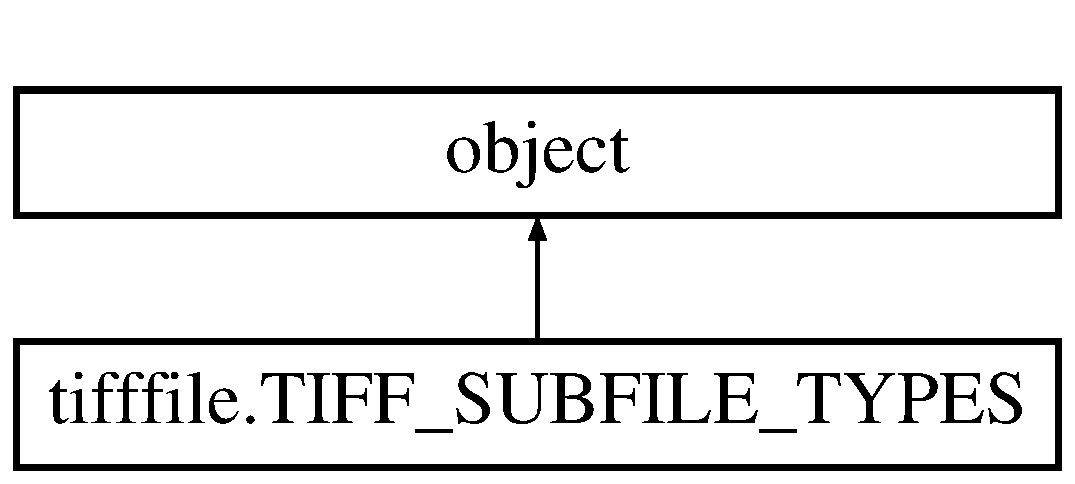
\includegraphics[height=2.000000cm]{classtifffile_1_1_t_i_f_f___s_u_b_f_i_l_e___t_y_p_e_s}
\end{center}
\end{figure}
\subsection*{Public Member Functions}
\begin{DoxyCompactItemize}
\item 
def \hyperlink{classtifffile_1_1_t_i_f_f___s_u_b_f_i_l_e___t_y_p_e_s_a64c992e0cabb37664338e4a7edfa34c8}{\-\_\-\-\_\-getitem\-\_\-\-\_\-}
\end{DoxyCompactItemize}


\subsection{Member Function Documentation}
\hypertarget{classtifffile_1_1_t_i_f_f___s_u_b_f_i_l_e___t_y_p_e_s_a64c992e0cabb37664338e4a7edfa34c8}{\index{tifffile\-::\-T\-I\-F\-F\-\_\-\-S\-U\-B\-F\-I\-L\-E\-\_\-\-T\-Y\-P\-E\-S@{tifffile\-::\-T\-I\-F\-F\-\_\-\-S\-U\-B\-F\-I\-L\-E\-\_\-\-T\-Y\-P\-E\-S}!\-\_\-\-\_\-getitem\-\_\-\-\_\-@{\-\_\-\-\_\-getitem\-\_\-\-\_\-}}
\index{\-\_\-\-\_\-getitem\-\_\-\-\_\-@{\-\_\-\-\_\-getitem\-\_\-\-\_\-}!tifffile::TIFF_SUBFILE_TYPES@{tifffile\-::\-T\-I\-F\-F\-\_\-\-S\-U\-B\-F\-I\-L\-E\-\_\-\-T\-Y\-P\-E\-S}}
\subsubsection[{\-\_\-\-\_\-getitem\-\_\-\-\_\-}]{\setlength{\rightskip}{0pt plus 5cm}def tifffile.\-T\-I\-F\-F\-\_\-\-S\-U\-B\-F\-I\-L\-E\-\_\-\-T\-Y\-P\-E\-S.\-\_\-\-\_\-getitem\-\_\-\-\_\- (
\begin{DoxyParamCaption}
\item[{}]{self, }
\item[{}]{key}
\end{DoxyParamCaption}
)}}\label{classtifffile_1_1_t_i_f_f___s_u_b_f_i_l_e___t_y_p_e_s_a64c992e0cabb37664338e4a7edfa34c8}


The documentation for this class was generated from the following file\-:\begin{DoxyCompactItemize}
\item 
workdir/atrex/\-Software/\hyperlink{tifffile_8py}{tifffile.\-py}\end{DoxyCompactItemize}

\hypertarget{classtifffile_1_1_tiff_file}{\section{tifffile.\-Tiff\-File Class Reference}
\label{classtifffile_1_1_tiff_file}\index{tifffile.\-Tiff\-File@{tifffile.\-Tiff\-File}}
}
Inheritance diagram for tifffile.\-Tiff\-File\-:\begin{figure}[H]
\begin{center}
\leavevmode
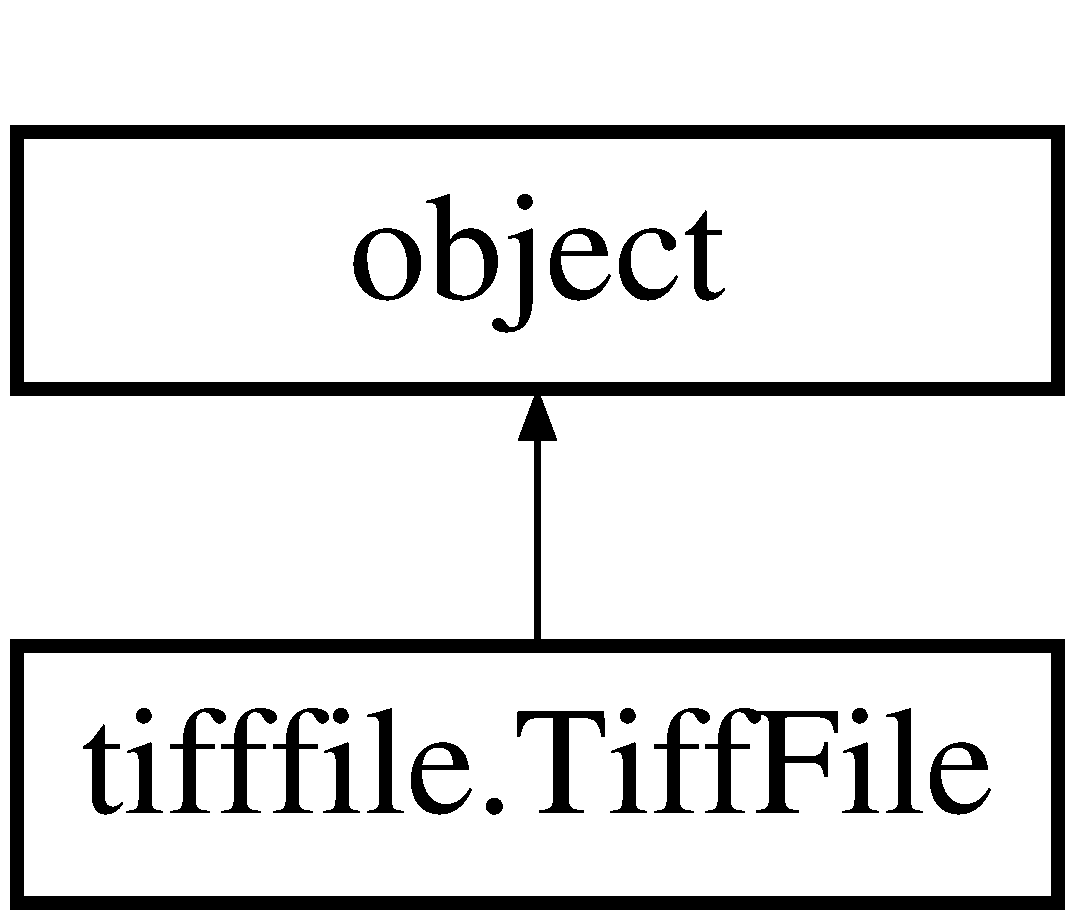
\includegraphics[height=2.000000cm]{classtifffile_1_1_tiff_file}
\end{center}
\end{figure}
\subsection*{Public Member Functions}
\begin{DoxyCompactItemize}
\item 
def \hyperlink{classtifffile_1_1_tiff_file_a2cacc91d936a85b866629e1004db56be}{\-\_\-\-\_\-init\-\_\-\-\_\-}
\item 
def \hyperlink{classtifffile_1_1_tiff_file_ab60b7755da796bc24e0959901a2178f2}{filehandle}
\item 
def \hyperlink{classtifffile_1_1_tiff_file_a6215683006e55ed5602df52a5596b6c2}{filename}
\item 
def \hyperlink{classtifffile_1_1_tiff_file_aeee11d1813bfd5ca6684468bb771f214}{close}
\item 
def \hyperlink{classtifffile_1_1_tiff_file_a774e670bd07b1bfc5f06ccd52a6a800a}{series}
\item 
def \hyperlink{classtifffile_1_1_tiff_file_a6ffb819278ba899e42fd6253508bcb8a}{asarray}
\item 
def \hyperlink{classtifffile_1_1_tiff_file_a9e400571d3475d5e268893877136bf24}{\-\_\-\-\_\-len\-\_\-\-\_\-}
\item 
def \hyperlink{classtifffile_1_1_tiff_file_addf7084c3ea60f31fa8f19b4db5284a4}{\-\_\-\-\_\-getitem\-\_\-\-\_\-}
\item 
def \hyperlink{classtifffile_1_1_tiff_file_a12847e8b06cb8c2c4b9233377eaec539}{\-\_\-\-\_\-iter\-\_\-\-\_\-}
\item 
def \hyperlink{classtifffile_1_1_tiff_file_a090018b858ceac412aafeae6c6c29a89}{\-\_\-\-\_\-str\-\_\-\-\_\-}
\item 
def \hyperlink{classtifffile_1_1_tiff_file_a8af0d38a6308893259f009a848dc8f55}{\-\_\-\-\_\-enter\-\_\-\-\_\-}
\item 
def \hyperlink{classtifffile_1_1_tiff_file_a86dacb85206d356ff3da93bec1ed0848}{\-\_\-\-\_\-exit\-\_\-\-\_\-}
\item 
def \hyperlink{classtifffile_1_1_tiff_file_a930a149ecaf1ad9409c4dbad1d9c2d60}{fstat}
\item 
def \hyperlink{classtifffile_1_1_tiff_file_af5d955e517896fee54d9fe3d9e9f266c}{is\-\_\-bigtiff}
\item 
def \hyperlink{classtifffile_1_1_tiff_file_a633ef6274a2c54e1af3f1e01c9e6ee66}{is\-\_\-rgb}
\item 
def \hyperlink{classtifffile_1_1_tiff_file_a610addce1bfe1fe31aed918f358bdeaf}{is\-\_\-palette}
\item 
def \hyperlink{classtifffile_1_1_tiff_file_a48749abc5c5eaf5e11cd731104c22cb9}{is\-\_\-mdgel}
\item 
def \hyperlink{classtifffile_1_1_tiff_file_a491c0c01ccff753773477ff0adc2b1c3}{is\-\_\-mediacy}
\item 
def \hyperlink{classtifffile_1_1_tiff_file_a3aef6d37c74dc3c2ae8d319f1680e4cd}{is\-\_\-stk}
\item 
def \hyperlink{classtifffile_1_1_tiff_file_a4b62231ac45a69f35b4eebe2cafd9233}{is\-\_\-lsm}
\item 
def \hyperlink{classtifffile_1_1_tiff_file_a57ccede80811571fa599f67771f35c6a}{is\-\_\-imagej}
\item 
def \hyperlink{classtifffile_1_1_tiff_file_a3ae5c2e4f211833e4d830c1af04b9b9f}{is\-\_\-micromanager}
\item 
def \hyperlink{classtifffile_1_1_tiff_file_a4b98fd0ade83b2679ecd2da1230196a1}{is\-\_\-nih}
\item 
def \hyperlink{classtifffile_1_1_tiff_file_a1f6562d875ce250d67b1566aaf49d9f7}{is\-\_\-fluoview}
\item 
def \hyperlink{classtifffile_1_1_tiff_file_acab85c4f4398924ad3cc041ef4beee90}{is\-\_\-ome}
\end{DoxyCompactItemize}
\subsection*{Public Attributes}
\begin{DoxyCompactItemize}
\item 
\hyperlink{classtifffile_1_1_tiff_file_ab531ab5699a9b426c32e26444e8e53ac}{offset\-\_\-size}
\item 
\hyperlink{classtifffile_1_1_tiff_file_a38687a2ea2711cef070cf0b9ddb4e65f}{pages}
\item 
\hyperlink{classtifffile_1_1_tiff_file_a9482f0d20fef11df3b9baaa04f8a7bb6}{byteorder}
\item 
\hyperlink{classtifffile_1_1_tiff_file_ad38661d0b0a16180347517d5ff208afd}{micromanager\-\_\-metadata}
\item 
\hyperlink{classtifffile_1_1_tiff_file_acc082b0de522251b75669336fe57b005}{master}
\item 
\hyperlink{classtifffile_1_1_tiff_file_a29b8b6eb049a61de92b16223f75492e0}{parent}
\end{DoxyCompactItemize}


\subsection{Detailed Description}
\begin{DoxyVerb}Read image and metadata from TIFF, STK, LSM, and FluoView files.

TiffFile instances must be closed using the close method, which is
automatically called when using the 'with' statement.

Attributes
----------
pages : list
    All TIFF pages in file.
series : list of Records(shape, dtype, axes, TiffPages)
    TIFF pages with compatible shapes and types.
micromanager_metadata: dict
    Extra MicroManager non-TIFF metadata in the file, if exists.

All attributes are read-only.

Examples
--------
>>> with TiffFile('test.tif') as tif:
...     data = tif.asarray()
...     data.shape
(256, 256, 4)\end{DoxyVerb}
 

\subsection{Constructor \& Destructor Documentation}
\hypertarget{classtifffile_1_1_tiff_file_a2cacc91d936a85b866629e1004db56be}{\index{tifffile\-::\-Tiff\-File@{tifffile\-::\-Tiff\-File}!\-\_\-\-\_\-init\-\_\-\-\_\-@{\-\_\-\-\_\-init\-\_\-\-\_\-}}
\index{\-\_\-\-\_\-init\-\_\-\-\_\-@{\-\_\-\-\_\-init\-\_\-\-\_\-}!tifffile::TiffFile@{tifffile\-::\-Tiff\-File}}
\subsubsection[{\-\_\-\-\_\-init\-\_\-\-\_\-}]{\setlength{\rightskip}{0pt plus 5cm}def tifffile.\-Tiff\-File.\-\_\-\-\_\-init\-\_\-\-\_\- (
\begin{DoxyParamCaption}
\item[{}]{self, }
\item[{}]{arg, }
\item[{}]{name = {\ttfamily None}, }
\item[{}]{offset = {\ttfamily None}, }
\item[{}]{size = {\ttfamily None}, }
\item[{}]{multifile = {\ttfamily True}, }
\item[{}]{multifile\-\_\-close = {\ttfamily True}}
\end{DoxyParamCaption}
)}}\label{classtifffile_1_1_tiff_file_a2cacc91d936a85b866629e1004db56be}
\begin{DoxyVerb}Initialize instance from file.

Parameters
----------
arg : str or open file
    Name of file or open file object.
    The file objects are closed in TiffFile.close().
name : str
    Optional name of file in case 'arg' is a file handle.
offset : int
    Optional start position of embedded file. By default this is
    the current file position.
size : int
    Optional size of embedded file. By default this is the number
    of bytes from the 'offset' to the end of the file.
multifile : bool
    If True (default), series may include pages from multiple files.
    Currently applies to OME-TIFF only.
multifile_close : bool
    If True (default), keep the handles of other files in multifile
    series closed. This is inefficient when few files refer to
    many pages. If False, the C runtime may run out of resources.\end{DoxyVerb}
 

\subsection{Member Function Documentation}
\hypertarget{classtifffile_1_1_tiff_file_a8af0d38a6308893259f009a848dc8f55}{\index{tifffile\-::\-Tiff\-File@{tifffile\-::\-Tiff\-File}!\-\_\-\-\_\-enter\-\_\-\-\_\-@{\-\_\-\-\_\-enter\-\_\-\-\_\-}}
\index{\-\_\-\-\_\-enter\-\_\-\-\_\-@{\-\_\-\-\_\-enter\-\_\-\-\_\-}!tifffile::TiffFile@{tifffile\-::\-Tiff\-File}}
\subsubsection[{\-\_\-\-\_\-enter\-\_\-\-\_\-}]{\setlength{\rightskip}{0pt plus 5cm}def tifffile.\-Tiff\-File.\-\_\-\-\_\-enter\-\_\-\-\_\- (
\begin{DoxyParamCaption}
\item[{}]{self}
\end{DoxyParamCaption}
)}}\label{classtifffile_1_1_tiff_file_a8af0d38a6308893259f009a848dc8f55}
\hypertarget{classtifffile_1_1_tiff_file_a86dacb85206d356ff3da93bec1ed0848}{\index{tifffile\-::\-Tiff\-File@{tifffile\-::\-Tiff\-File}!\-\_\-\-\_\-exit\-\_\-\-\_\-@{\-\_\-\-\_\-exit\-\_\-\-\_\-}}
\index{\-\_\-\-\_\-exit\-\_\-\-\_\-@{\-\_\-\-\_\-exit\-\_\-\-\_\-}!tifffile::TiffFile@{tifffile\-::\-Tiff\-File}}
\subsubsection[{\-\_\-\-\_\-exit\-\_\-\-\_\-}]{\setlength{\rightskip}{0pt plus 5cm}def tifffile.\-Tiff\-File.\-\_\-\-\_\-exit\-\_\-\-\_\- (
\begin{DoxyParamCaption}
\item[{}]{self, }
\item[{}]{exc\-\_\-type, }
\item[{}]{exc\-\_\-value, }
\item[{}]{traceback}
\end{DoxyParamCaption}
)}}\label{classtifffile_1_1_tiff_file_a86dacb85206d356ff3da93bec1ed0848}
\hypertarget{classtifffile_1_1_tiff_file_addf7084c3ea60f31fa8f19b4db5284a4}{\index{tifffile\-::\-Tiff\-File@{tifffile\-::\-Tiff\-File}!\-\_\-\-\_\-getitem\-\_\-\-\_\-@{\-\_\-\-\_\-getitem\-\_\-\-\_\-}}
\index{\-\_\-\-\_\-getitem\-\_\-\-\_\-@{\-\_\-\-\_\-getitem\-\_\-\-\_\-}!tifffile::TiffFile@{tifffile\-::\-Tiff\-File}}
\subsubsection[{\-\_\-\-\_\-getitem\-\_\-\-\_\-}]{\setlength{\rightskip}{0pt plus 5cm}def tifffile.\-Tiff\-File.\-\_\-\-\_\-getitem\-\_\-\-\_\- (
\begin{DoxyParamCaption}
\item[{}]{self, }
\item[{}]{key}
\end{DoxyParamCaption}
)}}\label{classtifffile_1_1_tiff_file_addf7084c3ea60f31fa8f19b4db5284a4}
\begin{DoxyVerb}Return specified page.\end{DoxyVerb}
 \hypertarget{classtifffile_1_1_tiff_file_a12847e8b06cb8c2c4b9233377eaec539}{\index{tifffile\-::\-Tiff\-File@{tifffile\-::\-Tiff\-File}!\-\_\-\-\_\-iter\-\_\-\-\_\-@{\-\_\-\-\_\-iter\-\_\-\-\_\-}}
\index{\-\_\-\-\_\-iter\-\_\-\-\_\-@{\-\_\-\-\_\-iter\-\_\-\-\_\-}!tifffile::TiffFile@{tifffile\-::\-Tiff\-File}}
\subsubsection[{\-\_\-\-\_\-iter\-\_\-\-\_\-}]{\setlength{\rightskip}{0pt plus 5cm}def tifffile.\-Tiff\-File.\-\_\-\-\_\-iter\-\_\-\-\_\- (
\begin{DoxyParamCaption}
\item[{}]{self}
\end{DoxyParamCaption}
)}}\label{classtifffile_1_1_tiff_file_a12847e8b06cb8c2c4b9233377eaec539}
\begin{DoxyVerb}Return iterator over pages.\end{DoxyVerb}
 \hypertarget{classtifffile_1_1_tiff_file_a9e400571d3475d5e268893877136bf24}{\index{tifffile\-::\-Tiff\-File@{tifffile\-::\-Tiff\-File}!\-\_\-\-\_\-len\-\_\-\-\_\-@{\-\_\-\-\_\-len\-\_\-\-\_\-}}
\index{\-\_\-\-\_\-len\-\_\-\-\_\-@{\-\_\-\-\_\-len\-\_\-\-\_\-}!tifffile::TiffFile@{tifffile\-::\-Tiff\-File}}
\subsubsection[{\-\_\-\-\_\-len\-\_\-\-\_\-}]{\setlength{\rightskip}{0pt plus 5cm}def tifffile.\-Tiff\-File.\-\_\-\-\_\-len\-\_\-\-\_\- (
\begin{DoxyParamCaption}
\item[{}]{self}
\end{DoxyParamCaption}
)}}\label{classtifffile_1_1_tiff_file_a9e400571d3475d5e268893877136bf24}
\begin{DoxyVerb}Return number of image pages in file.\end{DoxyVerb}
 \hypertarget{classtifffile_1_1_tiff_file_a090018b858ceac412aafeae6c6c29a89}{\index{tifffile\-::\-Tiff\-File@{tifffile\-::\-Tiff\-File}!\-\_\-\-\_\-str\-\_\-\-\_\-@{\-\_\-\-\_\-str\-\_\-\-\_\-}}
\index{\-\_\-\-\_\-str\-\_\-\-\_\-@{\-\_\-\-\_\-str\-\_\-\-\_\-}!tifffile::TiffFile@{tifffile\-::\-Tiff\-File}}
\subsubsection[{\-\_\-\-\_\-str\-\_\-\-\_\-}]{\setlength{\rightskip}{0pt plus 5cm}def tifffile.\-Tiff\-File.\-\_\-\-\_\-str\-\_\-\-\_\- (
\begin{DoxyParamCaption}
\item[{}]{self}
\end{DoxyParamCaption}
)}}\label{classtifffile_1_1_tiff_file_a090018b858ceac412aafeae6c6c29a89}
\begin{DoxyVerb}Return string containing information about file.\end{DoxyVerb}
 \hypertarget{classtifffile_1_1_tiff_file_a6ffb819278ba899e42fd6253508bcb8a}{\index{tifffile\-::\-Tiff\-File@{tifffile\-::\-Tiff\-File}!asarray@{asarray}}
\index{asarray@{asarray}!tifffile::TiffFile@{tifffile\-::\-Tiff\-File}}
\subsubsection[{asarray}]{\setlength{\rightskip}{0pt plus 5cm}def tifffile.\-Tiff\-File.\-asarray (
\begin{DoxyParamCaption}
\item[{}]{self, }
\item[{}]{key = {\ttfamily None}, }
\item[{}]{series = {\ttfamily None}, }
\item[{}]{memmap = {\ttfamily False}}
\end{DoxyParamCaption}
)}}\label{classtifffile_1_1_tiff_file_a6ffb819278ba899e42fd6253508bcb8a}
\begin{DoxyVerb}Return image data from multiple TIFF pages as numpy array.

By default the first image series is returned.

Parameters
----------
key : int, slice, or sequence of page indices
    Defines which pages to return as array.
series : int
    Defines which series of pages to return as array.
memmap : bool
    If True, return an array stored in a binary file on disk
    if possible.\end{DoxyVerb}
 \hypertarget{classtifffile_1_1_tiff_file_aeee11d1813bfd5ca6684468bb771f214}{\index{tifffile\-::\-Tiff\-File@{tifffile\-::\-Tiff\-File}!close@{close}}
\index{close@{close}!tifffile::TiffFile@{tifffile\-::\-Tiff\-File}}
\subsubsection[{close}]{\setlength{\rightskip}{0pt plus 5cm}def tifffile.\-Tiff\-File.\-close (
\begin{DoxyParamCaption}
\item[{}]{self}
\end{DoxyParamCaption}
)}}\label{classtifffile_1_1_tiff_file_aeee11d1813bfd5ca6684468bb771f214}
\begin{DoxyVerb}Close open file handle(s).\end{DoxyVerb}
 \hypertarget{classtifffile_1_1_tiff_file_ab60b7755da796bc24e0959901a2178f2}{\index{tifffile\-::\-Tiff\-File@{tifffile\-::\-Tiff\-File}!filehandle@{filehandle}}
\index{filehandle@{filehandle}!tifffile::TiffFile@{tifffile\-::\-Tiff\-File}}
\subsubsection[{filehandle}]{\setlength{\rightskip}{0pt plus 5cm}def tifffile.\-Tiff\-File.\-filehandle (
\begin{DoxyParamCaption}
\item[{}]{self}
\end{DoxyParamCaption}
)}}\label{classtifffile_1_1_tiff_file_ab60b7755da796bc24e0959901a2178f2}
\begin{DoxyVerb}Return file handle.\end{DoxyVerb}
 \hypertarget{classtifffile_1_1_tiff_file_a6215683006e55ed5602df52a5596b6c2}{\index{tifffile\-::\-Tiff\-File@{tifffile\-::\-Tiff\-File}!filename@{filename}}
\index{filename@{filename}!tifffile::TiffFile@{tifffile\-::\-Tiff\-File}}
\subsubsection[{filename}]{\setlength{\rightskip}{0pt plus 5cm}def tifffile.\-Tiff\-File.\-filename (
\begin{DoxyParamCaption}
\item[{}]{self}
\end{DoxyParamCaption}
)}}\label{classtifffile_1_1_tiff_file_a6215683006e55ed5602df52a5596b6c2}
\begin{DoxyVerb}Return name of file handle.\end{DoxyVerb}
 \hypertarget{classtifffile_1_1_tiff_file_a930a149ecaf1ad9409c4dbad1d9c2d60}{\index{tifffile\-::\-Tiff\-File@{tifffile\-::\-Tiff\-File}!fstat@{fstat}}
\index{fstat@{fstat}!tifffile::TiffFile@{tifffile\-::\-Tiff\-File}}
\subsubsection[{fstat}]{\setlength{\rightskip}{0pt plus 5cm}def tifffile.\-Tiff\-File.\-fstat (
\begin{DoxyParamCaption}
\item[{}]{self}
\end{DoxyParamCaption}
)}}\label{classtifffile_1_1_tiff_file_a930a149ecaf1ad9409c4dbad1d9c2d60}
\hypertarget{classtifffile_1_1_tiff_file_af5d955e517896fee54d9fe3d9e9f266c}{\index{tifffile\-::\-Tiff\-File@{tifffile\-::\-Tiff\-File}!is\-\_\-bigtiff@{is\-\_\-bigtiff}}
\index{is\-\_\-bigtiff@{is\-\_\-bigtiff}!tifffile::TiffFile@{tifffile\-::\-Tiff\-File}}
\subsubsection[{is\-\_\-bigtiff}]{\setlength{\rightskip}{0pt plus 5cm}def tifffile.\-Tiff\-File.\-is\-\_\-bigtiff (
\begin{DoxyParamCaption}
\item[{}]{self}
\end{DoxyParamCaption}
)}}\label{classtifffile_1_1_tiff_file_af5d955e517896fee54d9fe3d9e9f266c}
\hypertarget{classtifffile_1_1_tiff_file_a1f6562d875ce250d67b1566aaf49d9f7}{\index{tifffile\-::\-Tiff\-File@{tifffile\-::\-Tiff\-File}!is\-\_\-fluoview@{is\-\_\-fluoview}}
\index{is\-\_\-fluoview@{is\-\_\-fluoview}!tifffile::TiffFile@{tifffile\-::\-Tiff\-File}}
\subsubsection[{is\-\_\-fluoview}]{\setlength{\rightskip}{0pt plus 5cm}def tifffile.\-Tiff\-File.\-is\-\_\-fluoview (
\begin{DoxyParamCaption}
\item[{}]{self}
\end{DoxyParamCaption}
)}}\label{classtifffile_1_1_tiff_file_a1f6562d875ce250d67b1566aaf49d9f7}
\hypertarget{classtifffile_1_1_tiff_file_a57ccede80811571fa599f67771f35c6a}{\index{tifffile\-::\-Tiff\-File@{tifffile\-::\-Tiff\-File}!is\-\_\-imagej@{is\-\_\-imagej}}
\index{is\-\_\-imagej@{is\-\_\-imagej}!tifffile::TiffFile@{tifffile\-::\-Tiff\-File}}
\subsubsection[{is\-\_\-imagej}]{\setlength{\rightskip}{0pt plus 5cm}def tifffile.\-Tiff\-File.\-is\-\_\-imagej (
\begin{DoxyParamCaption}
\item[{}]{self}
\end{DoxyParamCaption}
)}}\label{classtifffile_1_1_tiff_file_a57ccede80811571fa599f67771f35c6a}
\hypertarget{classtifffile_1_1_tiff_file_a4b62231ac45a69f35b4eebe2cafd9233}{\index{tifffile\-::\-Tiff\-File@{tifffile\-::\-Tiff\-File}!is\-\_\-lsm@{is\-\_\-lsm}}
\index{is\-\_\-lsm@{is\-\_\-lsm}!tifffile::TiffFile@{tifffile\-::\-Tiff\-File}}
\subsubsection[{is\-\_\-lsm}]{\setlength{\rightskip}{0pt plus 5cm}def tifffile.\-Tiff\-File.\-is\-\_\-lsm (
\begin{DoxyParamCaption}
\item[{}]{self}
\end{DoxyParamCaption}
)}}\label{classtifffile_1_1_tiff_file_a4b62231ac45a69f35b4eebe2cafd9233}
\hypertarget{classtifffile_1_1_tiff_file_a48749abc5c5eaf5e11cd731104c22cb9}{\index{tifffile\-::\-Tiff\-File@{tifffile\-::\-Tiff\-File}!is\-\_\-mdgel@{is\-\_\-mdgel}}
\index{is\-\_\-mdgel@{is\-\_\-mdgel}!tifffile::TiffFile@{tifffile\-::\-Tiff\-File}}
\subsubsection[{is\-\_\-mdgel}]{\setlength{\rightskip}{0pt plus 5cm}def tifffile.\-Tiff\-File.\-is\-\_\-mdgel (
\begin{DoxyParamCaption}
\item[{}]{self}
\end{DoxyParamCaption}
)}}\label{classtifffile_1_1_tiff_file_a48749abc5c5eaf5e11cd731104c22cb9}
\hypertarget{classtifffile_1_1_tiff_file_a491c0c01ccff753773477ff0adc2b1c3}{\index{tifffile\-::\-Tiff\-File@{tifffile\-::\-Tiff\-File}!is\-\_\-mediacy@{is\-\_\-mediacy}}
\index{is\-\_\-mediacy@{is\-\_\-mediacy}!tifffile::TiffFile@{tifffile\-::\-Tiff\-File}}
\subsubsection[{is\-\_\-mediacy}]{\setlength{\rightskip}{0pt plus 5cm}def tifffile.\-Tiff\-File.\-is\-\_\-mediacy (
\begin{DoxyParamCaption}
\item[{}]{self}
\end{DoxyParamCaption}
)}}\label{classtifffile_1_1_tiff_file_a491c0c01ccff753773477ff0adc2b1c3}
\hypertarget{classtifffile_1_1_tiff_file_a3ae5c2e4f211833e4d830c1af04b9b9f}{\index{tifffile\-::\-Tiff\-File@{tifffile\-::\-Tiff\-File}!is\-\_\-micromanager@{is\-\_\-micromanager}}
\index{is\-\_\-micromanager@{is\-\_\-micromanager}!tifffile::TiffFile@{tifffile\-::\-Tiff\-File}}
\subsubsection[{is\-\_\-micromanager}]{\setlength{\rightskip}{0pt plus 5cm}def tifffile.\-Tiff\-File.\-is\-\_\-micromanager (
\begin{DoxyParamCaption}
\item[{}]{self}
\end{DoxyParamCaption}
)}}\label{classtifffile_1_1_tiff_file_a3ae5c2e4f211833e4d830c1af04b9b9f}
\hypertarget{classtifffile_1_1_tiff_file_a4b98fd0ade83b2679ecd2da1230196a1}{\index{tifffile\-::\-Tiff\-File@{tifffile\-::\-Tiff\-File}!is\-\_\-nih@{is\-\_\-nih}}
\index{is\-\_\-nih@{is\-\_\-nih}!tifffile::TiffFile@{tifffile\-::\-Tiff\-File}}
\subsubsection[{is\-\_\-nih}]{\setlength{\rightskip}{0pt plus 5cm}def tifffile.\-Tiff\-File.\-is\-\_\-nih (
\begin{DoxyParamCaption}
\item[{}]{self}
\end{DoxyParamCaption}
)}}\label{classtifffile_1_1_tiff_file_a4b98fd0ade83b2679ecd2da1230196a1}
\hypertarget{classtifffile_1_1_tiff_file_acab85c4f4398924ad3cc041ef4beee90}{\index{tifffile\-::\-Tiff\-File@{tifffile\-::\-Tiff\-File}!is\-\_\-ome@{is\-\_\-ome}}
\index{is\-\_\-ome@{is\-\_\-ome}!tifffile::TiffFile@{tifffile\-::\-Tiff\-File}}
\subsubsection[{is\-\_\-ome}]{\setlength{\rightskip}{0pt plus 5cm}def tifffile.\-Tiff\-File.\-is\-\_\-ome (
\begin{DoxyParamCaption}
\item[{}]{self}
\end{DoxyParamCaption}
)}}\label{classtifffile_1_1_tiff_file_acab85c4f4398924ad3cc041ef4beee90}
\hypertarget{classtifffile_1_1_tiff_file_a610addce1bfe1fe31aed918f358bdeaf}{\index{tifffile\-::\-Tiff\-File@{tifffile\-::\-Tiff\-File}!is\-\_\-palette@{is\-\_\-palette}}
\index{is\-\_\-palette@{is\-\_\-palette}!tifffile::TiffFile@{tifffile\-::\-Tiff\-File}}
\subsubsection[{is\-\_\-palette}]{\setlength{\rightskip}{0pt plus 5cm}def tifffile.\-Tiff\-File.\-is\-\_\-palette (
\begin{DoxyParamCaption}
\item[{}]{self}
\end{DoxyParamCaption}
)}}\label{classtifffile_1_1_tiff_file_a610addce1bfe1fe31aed918f358bdeaf}
\hypertarget{classtifffile_1_1_tiff_file_a633ef6274a2c54e1af3f1e01c9e6ee66}{\index{tifffile\-::\-Tiff\-File@{tifffile\-::\-Tiff\-File}!is\-\_\-rgb@{is\-\_\-rgb}}
\index{is\-\_\-rgb@{is\-\_\-rgb}!tifffile::TiffFile@{tifffile\-::\-Tiff\-File}}
\subsubsection[{is\-\_\-rgb}]{\setlength{\rightskip}{0pt plus 5cm}def tifffile.\-Tiff\-File.\-is\-\_\-rgb (
\begin{DoxyParamCaption}
\item[{}]{self}
\end{DoxyParamCaption}
)}}\label{classtifffile_1_1_tiff_file_a633ef6274a2c54e1af3f1e01c9e6ee66}
\hypertarget{classtifffile_1_1_tiff_file_a3aef6d37c74dc3c2ae8d319f1680e4cd}{\index{tifffile\-::\-Tiff\-File@{tifffile\-::\-Tiff\-File}!is\-\_\-stk@{is\-\_\-stk}}
\index{is\-\_\-stk@{is\-\_\-stk}!tifffile::TiffFile@{tifffile\-::\-Tiff\-File}}
\subsubsection[{is\-\_\-stk}]{\setlength{\rightskip}{0pt plus 5cm}def tifffile.\-Tiff\-File.\-is\-\_\-stk (
\begin{DoxyParamCaption}
\item[{}]{self}
\end{DoxyParamCaption}
)}}\label{classtifffile_1_1_tiff_file_a3aef6d37c74dc3c2ae8d319f1680e4cd}
\hypertarget{classtifffile_1_1_tiff_file_a774e670bd07b1bfc5f06ccd52a6a800a}{\index{tifffile\-::\-Tiff\-File@{tifffile\-::\-Tiff\-File}!series@{series}}
\index{series@{series}!tifffile::TiffFile@{tifffile\-::\-Tiff\-File}}
\subsubsection[{series}]{\setlength{\rightskip}{0pt plus 5cm}def tifffile.\-Tiff\-File.\-series (
\begin{DoxyParamCaption}
\item[{}]{self}
\end{DoxyParamCaption}
)}}\label{classtifffile_1_1_tiff_file_a774e670bd07b1bfc5f06ccd52a6a800a}
\begin{DoxyVerb}Return series of TiffPage with compatible shape and properties.\end{DoxyVerb}
 

\subsection{Member Data Documentation}
\hypertarget{classtifffile_1_1_tiff_file_a9482f0d20fef11df3b9baaa04f8a7bb6}{\index{tifffile\-::\-Tiff\-File@{tifffile\-::\-Tiff\-File}!byteorder@{byteorder}}
\index{byteorder@{byteorder}!tifffile::TiffFile@{tifffile\-::\-Tiff\-File}}
\subsubsection[{byteorder}]{\setlength{\rightskip}{0pt plus 5cm}tifffile.\-Tiff\-File.\-byteorder}}\label{classtifffile_1_1_tiff_file_a9482f0d20fef11df3b9baaa04f8a7bb6}
\hypertarget{classtifffile_1_1_tiff_file_acc082b0de522251b75669336fe57b005}{\index{tifffile\-::\-Tiff\-File@{tifffile\-::\-Tiff\-File}!master@{master}}
\index{master@{master}!tifffile::TiffFile@{tifffile\-::\-Tiff\-File}}
\subsubsection[{master}]{\setlength{\rightskip}{0pt plus 5cm}tifffile.\-Tiff\-File.\-master}}\label{classtifffile_1_1_tiff_file_acc082b0de522251b75669336fe57b005}
\hypertarget{classtifffile_1_1_tiff_file_ad38661d0b0a16180347517d5ff208afd}{\index{tifffile\-::\-Tiff\-File@{tifffile\-::\-Tiff\-File}!micromanager\-\_\-metadata@{micromanager\-\_\-metadata}}
\index{micromanager\-\_\-metadata@{micromanager\-\_\-metadata}!tifffile::TiffFile@{tifffile\-::\-Tiff\-File}}
\subsubsection[{micromanager\-\_\-metadata}]{\setlength{\rightskip}{0pt plus 5cm}tifffile.\-Tiff\-File.\-micromanager\-\_\-metadata}}\label{classtifffile_1_1_tiff_file_ad38661d0b0a16180347517d5ff208afd}
\hypertarget{classtifffile_1_1_tiff_file_ab531ab5699a9b426c32e26444e8e53ac}{\index{tifffile\-::\-Tiff\-File@{tifffile\-::\-Tiff\-File}!offset\-\_\-size@{offset\-\_\-size}}
\index{offset\-\_\-size@{offset\-\_\-size}!tifffile::TiffFile@{tifffile\-::\-Tiff\-File}}
\subsubsection[{offset\-\_\-size}]{\setlength{\rightskip}{0pt plus 5cm}tifffile.\-Tiff\-File.\-offset\-\_\-size}}\label{classtifffile_1_1_tiff_file_ab531ab5699a9b426c32e26444e8e53ac}
\hypertarget{classtifffile_1_1_tiff_file_a38687a2ea2711cef070cf0b9ddb4e65f}{\index{tifffile\-::\-Tiff\-File@{tifffile\-::\-Tiff\-File}!pages@{pages}}
\index{pages@{pages}!tifffile::TiffFile@{tifffile\-::\-Tiff\-File}}
\subsubsection[{pages}]{\setlength{\rightskip}{0pt plus 5cm}tifffile.\-Tiff\-File.\-pages}}\label{classtifffile_1_1_tiff_file_a38687a2ea2711cef070cf0b9ddb4e65f}
\hypertarget{classtifffile_1_1_tiff_file_a29b8b6eb049a61de92b16223f75492e0}{\index{tifffile\-::\-Tiff\-File@{tifffile\-::\-Tiff\-File}!parent@{parent}}
\index{parent@{parent}!tifffile::TiffFile@{tifffile\-::\-Tiff\-File}}
\subsubsection[{parent}]{\setlength{\rightskip}{0pt plus 5cm}tifffile.\-Tiff\-File.\-parent}}\label{classtifffile_1_1_tiff_file_a29b8b6eb049a61de92b16223f75492e0}


The documentation for this class was generated from the following file\-:\begin{DoxyCompactItemize}
\item 
workdir/atrex/\-Software/\hyperlink{tifffile_8py}{tifffile.\-py}\end{DoxyCompactItemize}

\hypertarget{classtifffile_1_1_tiff_page}{\section{tifffile.\-Tiff\-Page Class Reference}
\label{classtifffile_1_1_tiff_page}\index{tifffile.\-Tiff\-Page@{tifffile.\-Tiff\-Page}}
}
Inheritance diagram for tifffile.\-Tiff\-Page\-:\begin{figure}[H]
\begin{center}
\leavevmode
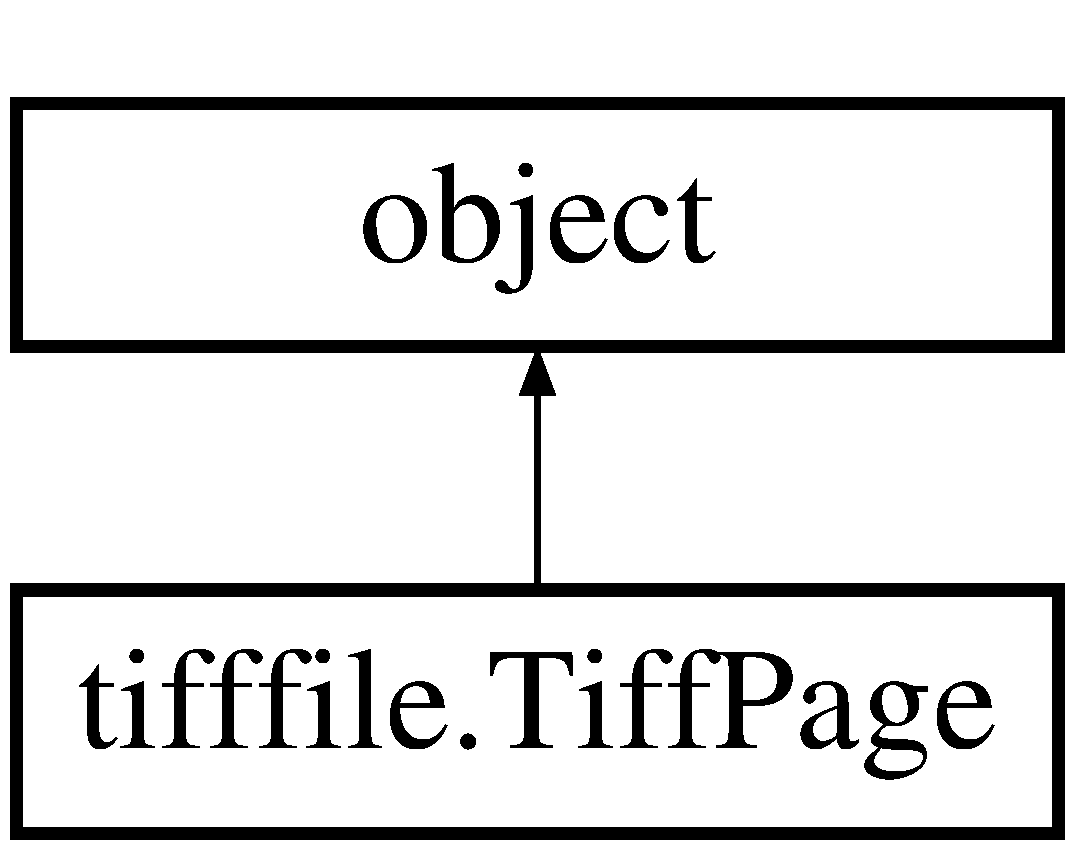
\includegraphics[height=2.000000cm]{classtifffile_1_1_tiff_page}
\end{center}
\end{figure}
\subsection*{Public Member Functions}
\begin{DoxyCompactItemize}
\item 
def \hyperlink{classtifffile_1_1_tiff_page_a91ce69df8f42151984d02d4054908c13}{\-\_\-\-\_\-init\-\_\-\-\_\-}
\item 
def \hyperlink{classtifffile_1_1_tiff_page_a5953a258881256d704bd3d0c34a09bea}{asarray}
\item 
def \hyperlink{classtifffile_1_1_tiff_page_ad0679ea4c15ca29548ae87e4986a7811}{is\-\_\-contiguous}
\item 
def \hyperlink{classtifffile_1_1_tiff_page_af0e5e72edfa67d9f1239b194cbd7a56b}{\-\_\-\-\_\-str\-\_\-\-\_\-}
\item 
def \hyperlink{classtifffile_1_1_tiff_page_a43cd8883f12805d887c2994582110e42}{\-\_\-\-\_\-getattr\-\_\-\-\_\-}
\item 
def \hyperlink{classtifffile_1_1_tiff_page_a56fb86bb7966d84b7b72d1edc297eaed}{uic\-\_\-tags}
\item 
def \hyperlink{classtifffile_1_1_tiff_page_acd582c08af3fc15fa22bbc4f6b7d4a4d}{imagej\-\_\-tags}
\item 
def \hyperlink{classtifffile_1_1_tiff_page_aad80ffe0eb6611da60f78ad2743298a0}{is\-\_\-rgb}
\item 
def \hyperlink{classtifffile_1_1_tiff_page_a1af194b01da49777e8d7585a987f6ccf}{is\-\_\-contig}
\item 
def \hyperlink{classtifffile_1_1_tiff_page_aca723b525070789164837eb2ce3b366f}{is\-\_\-palette}
\item 
def \hyperlink{classtifffile_1_1_tiff_page_afcf12e643a6207d0a02184ab19485489}{is\-\_\-tiled}
\item 
def \hyperlink{classtifffile_1_1_tiff_page_af5f9892583d02082fd1be22ebe653a28}{is\-\_\-reduced}
\item 
def \hyperlink{classtifffile_1_1_tiff_page_a11f2d006bbe32f212252c65a9bb9adcb}{is\-\_\-mdgel}
\item 
def \hyperlink{classtifffile_1_1_tiff_page_a664758db65e7865792cc53dd01946054}{is\-\_\-mediacy}
\item 
def \hyperlink{classtifffile_1_1_tiff_page_a7e17dfd14c887008863f4f800e701df1}{is\-\_\-stk}
\item 
def \hyperlink{classtifffile_1_1_tiff_page_a22c271c0c693e40335409c006dc6fb0b}{is\-\_\-lsm}
\item 
def \hyperlink{classtifffile_1_1_tiff_page_ab0fab509161b423ac295e4e9b1944c86}{is\-\_\-fluoview}
\item 
def \hyperlink{classtifffile_1_1_tiff_page_acb4272f79554d1ca0095eb632b7a6f3b}{is\-\_\-nih}
\item 
def \hyperlink{classtifffile_1_1_tiff_page_a107d6251fcd55df6f56ce4defeeb708d}{is\-\_\-sgi}
\item 
def \hyperlink{classtifffile_1_1_tiff_page_a38427d4854f650021214d82f25618b98}{is\-\_\-ome}
\item 
def \hyperlink{classtifffile_1_1_tiff_page_a81ea5ec5d4571a149c7217b20582873f}{is\-\_\-shaped}
\item 
def \hyperlink{classtifffile_1_1_tiff_page_ada0d8196ba5f814cd827021a7cee5d1f}{is\-\_\-imagej}
\item 
def \hyperlink{classtifffile_1_1_tiff_page_a792d201ffbca69b7324ecb654f0faed2}{is\-\_\-micromanager}
\end{DoxyCompactItemize}
\subsection*{Public Attributes}
\begin{DoxyCompactItemize}
\item 
\hyperlink{classtifffile_1_1_tiff_page_ab448d691bfba9af88ba2658afc1b8607}{parent}
\item 
\hyperlink{classtifffile_1_1_tiff_page_abcdadcc105890e623a2ce56877d74c6d}{index}
\item 
\hyperlink{classtifffile_1_1_tiff_page_af842924ca07e0f250d2ffdcbbf1afee1}{shape}
\item 
\hyperlink{classtifffile_1_1_tiff_page_ad49c26fc7bb2cfa901aa5664879bee65}{dtype}
\item 
\hyperlink{classtifffile_1_1_tiff_page_ac28c18fcf1ee6655eaaaf035a34c9d67}{axes}
\item 
\hyperlink{classtifffile_1_1_tiff_page_aa35f477474445140346421065a4c016b}{tags}
\item 
\hyperlink{classtifffile_1_1_tiff_page_a04d82b99a53cb0b445162c2e5138d136}{bits\-\_\-per\-\_\-sample}
\item 
\hyperlink{classtifffile_1_1_tiff_page_aef04ecb2f6f230925aeb43ac3b89e30d}{sample\-\_\-format}
\item 
\hyperlink{classtifffile_1_1_tiff_page_af115186598b38bc4390942115755f7b6}{photometric}
\item 
\hyperlink{classtifffile_1_1_tiff_page_ac119ed52ce81ef4997ada9444c39562e}{image\-\_\-depth}
\item 
\hyperlink{classtifffile_1_1_tiff_page_a2c728cfc9795dc4bf187308d551cecb1}{strips\-\_\-per\-\_\-image}
\item 
\hyperlink{classtifffile_1_1_tiff_page_aa98d8b1ccceb95ebd19896249f9f4796}{image\-\_\-length}
\item 
\hyperlink{classtifffile_1_1_tiff_page_aa16948ea525cd29705c896e1451290fa}{image\-\_\-width}
\item 
\hyperlink{classtifffile_1_1_tiff_page_aa3c254120ad8e9394ecb5c743ebf7434}{strip\-\_\-offsets}
\item 
\hyperlink{classtifffile_1_1_tiff_page_a58f5c25b8b86eb6c9a5b393e9d43c2f4}{color\-\_\-map}
\item 
\hyperlink{classtifffile_1_1_tiff_page_a376e981b0117a1be89cf336c317fd6cd}{is\-\_\-palette}
\item 
\hyperlink{classtifffile_1_1_tiff_page_ac55af94dba8786edaf1e89d205aed908}{strip\-\_\-byte\-\_\-counts}
\item 
\hyperlink{classtifffile_1_1_tiff_page_af35a60f003687668b066628dc8a1c1b5}{compression}
\item 
\hyperlink{classtifffile_1_1_tiff_page_ad51af99f663803ce6f02e124bb2db690}{predictor}
\end{DoxyCompactItemize}


\subsection{Detailed Description}
\begin{DoxyVerb}A TIFF image file directory (IFD).

Attributes
----------
index : int
    Index of page in file.
dtype : str {TIFF_SAMPLE_DTYPES}
    Data type of image, colormapped if applicable.
shape : tuple
    Dimensions of the image array in TIFF page,
    colormapped and with one alpha channel if applicable.
axes : str
    Axes label codes:
    'X' width, 'Y' height, 'S' sample, 'I' image series|page|plane,
    'Z' depth, 'C' color|em-wavelength|channel, 'E' ex-wavelength|lambda,
    'T' time, 'R' region|tile, 'A' angle, 'P' phase, 'H' lifetime,
    'L' exposure, 'V' event, 'Q' unknown, '_' missing
tags : TiffTags
    Dictionary of tags in page.
    Tag values are also directly accessible as attributes.
color_map : numpy array
    Color look up table, if exists.
cz_lsm_scan_info: Record(dict)
    LSM scan info attributes, if exists.
imagej_tags: Record(dict)
    Consolidated ImageJ description and metadata tags, if exists.
uic_tags: Record(dict)
    Consolidated MetaMorph STK/UIC tags, if exists.

All attributes are read-only.

Notes
-----
The internal, normalized '_shape' attribute is 6 dimensional:

0. number planes  (stk)
1. planar samples_per_pixel
2. image_depth Z  (sgi)
3. image_length Y
4. image_width X
5. contig samples_per_pixel\end{DoxyVerb}
 

\subsection{Constructor \& Destructor Documentation}
\hypertarget{classtifffile_1_1_tiff_page_a91ce69df8f42151984d02d4054908c13}{\index{tifffile\-::\-Tiff\-Page@{tifffile\-::\-Tiff\-Page}!\-\_\-\-\_\-init\-\_\-\-\_\-@{\-\_\-\-\_\-init\-\_\-\-\_\-}}
\index{\-\_\-\-\_\-init\-\_\-\-\_\-@{\-\_\-\-\_\-init\-\_\-\-\_\-}!tifffile::TiffPage@{tifffile\-::\-Tiff\-Page}}
\subsubsection[{\-\_\-\-\_\-init\-\_\-\-\_\-}]{\setlength{\rightskip}{0pt plus 5cm}def tifffile.\-Tiff\-Page.\-\_\-\-\_\-init\-\_\-\-\_\- (
\begin{DoxyParamCaption}
\item[{}]{self, }
\item[{}]{parent}
\end{DoxyParamCaption}
)}}\label{classtifffile_1_1_tiff_page_a91ce69df8f42151984d02d4054908c13}
\begin{DoxyVerb}Initialize instance from file.\end{DoxyVerb}
 

\subsection{Member Function Documentation}
\hypertarget{classtifffile_1_1_tiff_page_a43cd8883f12805d887c2994582110e42}{\index{tifffile\-::\-Tiff\-Page@{tifffile\-::\-Tiff\-Page}!\-\_\-\-\_\-getattr\-\_\-\-\_\-@{\-\_\-\-\_\-getattr\-\_\-\-\_\-}}
\index{\-\_\-\-\_\-getattr\-\_\-\-\_\-@{\-\_\-\-\_\-getattr\-\_\-\-\_\-}!tifffile::TiffPage@{tifffile\-::\-Tiff\-Page}}
\subsubsection[{\-\_\-\-\_\-getattr\-\_\-\-\_\-}]{\setlength{\rightskip}{0pt plus 5cm}def tifffile.\-Tiff\-Page.\-\_\-\-\_\-getattr\-\_\-\-\_\- (
\begin{DoxyParamCaption}
\item[{}]{self, }
\item[{}]{name}
\end{DoxyParamCaption}
)}}\label{classtifffile_1_1_tiff_page_a43cd8883f12805d887c2994582110e42}
\begin{DoxyVerb}Return tag value.\end{DoxyVerb}
 \hypertarget{classtifffile_1_1_tiff_page_af0e5e72edfa67d9f1239b194cbd7a56b}{\index{tifffile\-::\-Tiff\-Page@{tifffile\-::\-Tiff\-Page}!\-\_\-\-\_\-str\-\_\-\-\_\-@{\-\_\-\-\_\-str\-\_\-\-\_\-}}
\index{\-\_\-\-\_\-str\-\_\-\-\_\-@{\-\_\-\-\_\-str\-\_\-\-\_\-}!tifffile::TiffPage@{tifffile\-::\-Tiff\-Page}}
\subsubsection[{\-\_\-\-\_\-str\-\_\-\-\_\-}]{\setlength{\rightskip}{0pt plus 5cm}def tifffile.\-Tiff\-Page.\-\_\-\-\_\-str\-\_\-\-\_\- (
\begin{DoxyParamCaption}
\item[{}]{self}
\end{DoxyParamCaption}
)}}\label{classtifffile_1_1_tiff_page_af0e5e72edfa67d9f1239b194cbd7a56b}
\begin{DoxyVerb}Return string containing information about page.\end{DoxyVerb}
 \hypertarget{classtifffile_1_1_tiff_page_a5953a258881256d704bd3d0c34a09bea}{\index{tifffile\-::\-Tiff\-Page@{tifffile\-::\-Tiff\-Page}!asarray@{asarray}}
\index{asarray@{asarray}!tifffile::TiffPage@{tifffile\-::\-Tiff\-Page}}
\subsubsection[{asarray}]{\setlength{\rightskip}{0pt plus 5cm}def tifffile.\-Tiff\-Page.\-asarray (
\begin{DoxyParamCaption}
\item[{}]{self, }
\item[{}]{squeeze = {\ttfamily True}, }
\item[{}]{colormapped = {\ttfamily True}, }
\item[{}]{rgbonly = {\ttfamily False}, }
\item[{}]{scale\-\_\-mdgel = {\ttfamily False}, }
\item[{}]{memmap = {\ttfamily False}, }
\item[{}]{reopen = {\ttfamily True}}
\end{DoxyParamCaption}
)}}\label{classtifffile_1_1_tiff_page_a5953a258881256d704bd3d0c34a09bea}
\begin{DoxyVerb}Read image data from file and return as numpy array.

Raise ValueError if format is unsupported.
If any of 'squeeze', 'colormapped', or 'rgbonly' are not the default,
the shape of the returned array might be different from the page shape.

Parameters
----------
squeeze : bool
    If True, all length-1 dimensions (except X and Y) are
    squeezed out from result.
colormapped : bool
    If True, color mapping is applied for palette-indexed images.
rgbonly : bool
    If True, return RGB(A) image without additional extra samples.
memmap : bool
    If True, use numpy.memmap to read arrays from file if possible.
    For use on 64 bit systems and files with few huge contiguous data.
reopen : bool
    If True and the parent file handle is closed, the file is
    temporarily re-opened (and closed if no exception occurs).
scale_mdgel : bool
    If True, MD Gel data will be scaled according to the private
    metadata in the second TIFF page. The dtype will be float32.\end{DoxyVerb}
 \hypertarget{classtifffile_1_1_tiff_page_acd582c08af3fc15fa22bbc4f6b7d4a4d}{\index{tifffile\-::\-Tiff\-Page@{tifffile\-::\-Tiff\-Page}!imagej\-\_\-tags@{imagej\-\_\-tags}}
\index{imagej\-\_\-tags@{imagej\-\_\-tags}!tifffile::TiffPage@{tifffile\-::\-Tiff\-Page}}
\subsubsection[{imagej\-\_\-tags}]{\setlength{\rightskip}{0pt plus 5cm}def tifffile.\-Tiff\-Page.\-imagej\-\_\-tags (
\begin{DoxyParamCaption}
\item[{}]{self}
\end{DoxyParamCaption}
)}}\label{classtifffile_1_1_tiff_page_acd582c08af3fc15fa22bbc4f6b7d4a4d}
\begin{DoxyVerb}Consolidate ImageJ metadata.\end{DoxyVerb}
 \hypertarget{classtifffile_1_1_tiff_page_a1af194b01da49777e8d7585a987f6ccf}{\index{tifffile\-::\-Tiff\-Page@{tifffile\-::\-Tiff\-Page}!is\-\_\-contig@{is\-\_\-contig}}
\index{is\-\_\-contig@{is\-\_\-contig}!tifffile::TiffPage@{tifffile\-::\-Tiff\-Page}}
\subsubsection[{is\-\_\-contig}]{\setlength{\rightskip}{0pt plus 5cm}def tifffile.\-Tiff\-Page.\-is\-\_\-contig (
\begin{DoxyParamCaption}
\item[{}]{self}
\end{DoxyParamCaption}
)}}\label{classtifffile_1_1_tiff_page_a1af194b01da49777e8d7585a987f6ccf}
\begin{DoxyVerb}True if page contains a contiguous image.\end{DoxyVerb}
 \hypertarget{classtifffile_1_1_tiff_page_ad0679ea4c15ca29548ae87e4986a7811}{\index{tifffile\-::\-Tiff\-Page@{tifffile\-::\-Tiff\-Page}!is\-\_\-contiguous@{is\-\_\-contiguous}}
\index{is\-\_\-contiguous@{is\-\_\-contiguous}!tifffile::TiffPage@{tifffile\-::\-Tiff\-Page}}
\subsubsection[{is\-\_\-contiguous}]{\setlength{\rightskip}{0pt plus 5cm}def tifffile.\-Tiff\-Page.\-is\-\_\-contiguous (
\begin{DoxyParamCaption}
\item[{}]{self}
\end{DoxyParamCaption}
)}}\label{classtifffile_1_1_tiff_page_ad0679ea4c15ca29548ae87e4986a7811}
\begin{DoxyVerb}Return offset and size of contiguous data, else None.

Excludes prediction and colormapping.\end{DoxyVerb}
 \hypertarget{classtifffile_1_1_tiff_page_ab0fab509161b423ac295e4e9b1944c86}{\index{tifffile\-::\-Tiff\-Page@{tifffile\-::\-Tiff\-Page}!is\-\_\-fluoview@{is\-\_\-fluoview}}
\index{is\-\_\-fluoview@{is\-\_\-fluoview}!tifffile::TiffPage@{tifffile\-::\-Tiff\-Page}}
\subsubsection[{is\-\_\-fluoview}]{\setlength{\rightskip}{0pt plus 5cm}def tifffile.\-Tiff\-Page.\-is\-\_\-fluoview (
\begin{DoxyParamCaption}
\item[{}]{self}
\end{DoxyParamCaption}
)}}\label{classtifffile_1_1_tiff_page_ab0fab509161b423ac295e4e9b1944c86}
\begin{DoxyVerb}True if page contains FluoView MM_STAMP tag.\end{DoxyVerb}
 \hypertarget{classtifffile_1_1_tiff_page_ada0d8196ba5f814cd827021a7cee5d1f}{\index{tifffile\-::\-Tiff\-Page@{tifffile\-::\-Tiff\-Page}!is\-\_\-imagej@{is\-\_\-imagej}}
\index{is\-\_\-imagej@{is\-\_\-imagej}!tifffile::TiffPage@{tifffile\-::\-Tiff\-Page}}
\subsubsection[{is\-\_\-imagej}]{\setlength{\rightskip}{0pt plus 5cm}def tifffile.\-Tiff\-Page.\-is\-\_\-imagej (
\begin{DoxyParamCaption}
\item[{}]{self}
\end{DoxyParamCaption}
)}}\label{classtifffile_1_1_tiff_page_ada0d8196ba5f814cd827021a7cee5d1f}
\begin{DoxyVerb}True if page contains ImageJ description.\end{DoxyVerb}
 \hypertarget{classtifffile_1_1_tiff_page_a22c271c0c693e40335409c006dc6fb0b}{\index{tifffile\-::\-Tiff\-Page@{tifffile\-::\-Tiff\-Page}!is\-\_\-lsm@{is\-\_\-lsm}}
\index{is\-\_\-lsm@{is\-\_\-lsm}!tifffile::TiffPage@{tifffile\-::\-Tiff\-Page}}
\subsubsection[{is\-\_\-lsm}]{\setlength{\rightskip}{0pt plus 5cm}def tifffile.\-Tiff\-Page.\-is\-\_\-lsm (
\begin{DoxyParamCaption}
\item[{}]{self}
\end{DoxyParamCaption}
)}}\label{classtifffile_1_1_tiff_page_a22c271c0c693e40335409c006dc6fb0b}
\begin{DoxyVerb}True if page contains LSM CZ_LSM_INFO tag.\end{DoxyVerb}
 \hypertarget{classtifffile_1_1_tiff_page_a11f2d006bbe32f212252c65a9bb9adcb}{\index{tifffile\-::\-Tiff\-Page@{tifffile\-::\-Tiff\-Page}!is\-\_\-mdgel@{is\-\_\-mdgel}}
\index{is\-\_\-mdgel@{is\-\_\-mdgel}!tifffile::TiffPage@{tifffile\-::\-Tiff\-Page}}
\subsubsection[{is\-\_\-mdgel}]{\setlength{\rightskip}{0pt plus 5cm}def tifffile.\-Tiff\-Page.\-is\-\_\-mdgel (
\begin{DoxyParamCaption}
\item[{}]{self}
\end{DoxyParamCaption}
)}}\label{classtifffile_1_1_tiff_page_a11f2d006bbe32f212252c65a9bb9adcb}
\begin{DoxyVerb}True if page contains md_file_tag tag.\end{DoxyVerb}
 \hypertarget{classtifffile_1_1_tiff_page_a664758db65e7865792cc53dd01946054}{\index{tifffile\-::\-Tiff\-Page@{tifffile\-::\-Tiff\-Page}!is\-\_\-mediacy@{is\-\_\-mediacy}}
\index{is\-\_\-mediacy@{is\-\_\-mediacy}!tifffile::TiffPage@{tifffile\-::\-Tiff\-Page}}
\subsubsection[{is\-\_\-mediacy}]{\setlength{\rightskip}{0pt plus 5cm}def tifffile.\-Tiff\-Page.\-is\-\_\-mediacy (
\begin{DoxyParamCaption}
\item[{}]{self}
\end{DoxyParamCaption}
)}}\label{classtifffile_1_1_tiff_page_a664758db65e7865792cc53dd01946054}
\begin{DoxyVerb}True if page contains Media Cybernetics Id tag.\end{DoxyVerb}
 \hypertarget{classtifffile_1_1_tiff_page_a792d201ffbca69b7324ecb654f0faed2}{\index{tifffile\-::\-Tiff\-Page@{tifffile\-::\-Tiff\-Page}!is\-\_\-micromanager@{is\-\_\-micromanager}}
\index{is\-\_\-micromanager@{is\-\_\-micromanager}!tifffile::TiffPage@{tifffile\-::\-Tiff\-Page}}
\subsubsection[{is\-\_\-micromanager}]{\setlength{\rightskip}{0pt plus 5cm}def tifffile.\-Tiff\-Page.\-is\-\_\-micromanager (
\begin{DoxyParamCaption}
\item[{}]{self}
\end{DoxyParamCaption}
)}}\label{classtifffile_1_1_tiff_page_a792d201ffbca69b7324ecb654f0faed2}
\begin{DoxyVerb}True if page contains Micro-Manager metadata.\end{DoxyVerb}
 \hypertarget{classtifffile_1_1_tiff_page_acb4272f79554d1ca0095eb632b7a6f3b}{\index{tifffile\-::\-Tiff\-Page@{tifffile\-::\-Tiff\-Page}!is\-\_\-nih@{is\-\_\-nih}}
\index{is\-\_\-nih@{is\-\_\-nih}!tifffile::TiffPage@{tifffile\-::\-Tiff\-Page}}
\subsubsection[{is\-\_\-nih}]{\setlength{\rightskip}{0pt plus 5cm}def tifffile.\-Tiff\-Page.\-is\-\_\-nih (
\begin{DoxyParamCaption}
\item[{}]{self}
\end{DoxyParamCaption}
)}}\label{classtifffile_1_1_tiff_page_acb4272f79554d1ca0095eb632b7a6f3b}
\begin{DoxyVerb}True if page contains NIH image header.\end{DoxyVerb}
 \hypertarget{classtifffile_1_1_tiff_page_a38427d4854f650021214d82f25618b98}{\index{tifffile\-::\-Tiff\-Page@{tifffile\-::\-Tiff\-Page}!is\-\_\-ome@{is\-\_\-ome}}
\index{is\-\_\-ome@{is\-\_\-ome}!tifffile::TiffPage@{tifffile\-::\-Tiff\-Page}}
\subsubsection[{is\-\_\-ome}]{\setlength{\rightskip}{0pt plus 5cm}def tifffile.\-Tiff\-Page.\-is\-\_\-ome (
\begin{DoxyParamCaption}
\item[{}]{self}
\end{DoxyParamCaption}
)}}\label{classtifffile_1_1_tiff_page_a38427d4854f650021214d82f25618b98}
\begin{DoxyVerb}True if page contains OME-XML in image_description tag.\end{DoxyVerb}
 \hypertarget{classtifffile_1_1_tiff_page_aca723b525070789164837eb2ce3b366f}{\index{tifffile\-::\-Tiff\-Page@{tifffile\-::\-Tiff\-Page}!is\-\_\-palette@{is\-\_\-palette}}
\index{is\-\_\-palette@{is\-\_\-palette}!tifffile::TiffPage@{tifffile\-::\-Tiff\-Page}}
\subsubsection[{is\-\_\-palette}]{\setlength{\rightskip}{0pt plus 5cm}def tifffile.\-Tiff\-Page.\-is\-\_\-palette (
\begin{DoxyParamCaption}
\item[{}]{self}
\end{DoxyParamCaption}
)}}\label{classtifffile_1_1_tiff_page_aca723b525070789164837eb2ce3b366f}
\begin{DoxyVerb}True if page contains a palette-colored image and not OME or STK.\end{DoxyVerb}
 \hypertarget{classtifffile_1_1_tiff_page_af5f9892583d02082fd1be22ebe653a28}{\index{tifffile\-::\-Tiff\-Page@{tifffile\-::\-Tiff\-Page}!is\-\_\-reduced@{is\-\_\-reduced}}
\index{is\-\_\-reduced@{is\-\_\-reduced}!tifffile::TiffPage@{tifffile\-::\-Tiff\-Page}}
\subsubsection[{is\-\_\-reduced}]{\setlength{\rightskip}{0pt plus 5cm}def tifffile.\-Tiff\-Page.\-is\-\_\-reduced (
\begin{DoxyParamCaption}
\item[{}]{self}
\end{DoxyParamCaption}
)}}\label{classtifffile_1_1_tiff_page_af5f9892583d02082fd1be22ebe653a28}
\begin{DoxyVerb}True if page is a reduced image of another image.\end{DoxyVerb}
 \hypertarget{classtifffile_1_1_tiff_page_aad80ffe0eb6611da60f78ad2743298a0}{\index{tifffile\-::\-Tiff\-Page@{tifffile\-::\-Tiff\-Page}!is\-\_\-rgb@{is\-\_\-rgb}}
\index{is\-\_\-rgb@{is\-\_\-rgb}!tifffile::TiffPage@{tifffile\-::\-Tiff\-Page}}
\subsubsection[{is\-\_\-rgb}]{\setlength{\rightskip}{0pt plus 5cm}def tifffile.\-Tiff\-Page.\-is\-\_\-rgb (
\begin{DoxyParamCaption}
\item[{}]{self}
\end{DoxyParamCaption}
)}}\label{classtifffile_1_1_tiff_page_aad80ffe0eb6611da60f78ad2743298a0}
\begin{DoxyVerb}True if page contains a RGB image.\end{DoxyVerb}
 \hypertarget{classtifffile_1_1_tiff_page_a107d6251fcd55df6f56ce4defeeb708d}{\index{tifffile\-::\-Tiff\-Page@{tifffile\-::\-Tiff\-Page}!is\-\_\-sgi@{is\-\_\-sgi}}
\index{is\-\_\-sgi@{is\-\_\-sgi}!tifffile::TiffPage@{tifffile\-::\-Tiff\-Page}}
\subsubsection[{is\-\_\-sgi}]{\setlength{\rightskip}{0pt plus 5cm}def tifffile.\-Tiff\-Page.\-is\-\_\-sgi (
\begin{DoxyParamCaption}
\item[{}]{self}
\end{DoxyParamCaption}
)}}\label{classtifffile_1_1_tiff_page_a107d6251fcd55df6f56ce4defeeb708d}
\begin{DoxyVerb}True if page contains SGI image and tile depth tags.\end{DoxyVerb}
 \hypertarget{classtifffile_1_1_tiff_page_a81ea5ec5d4571a149c7217b20582873f}{\index{tifffile\-::\-Tiff\-Page@{tifffile\-::\-Tiff\-Page}!is\-\_\-shaped@{is\-\_\-shaped}}
\index{is\-\_\-shaped@{is\-\_\-shaped}!tifffile::TiffPage@{tifffile\-::\-Tiff\-Page}}
\subsubsection[{is\-\_\-shaped}]{\setlength{\rightskip}{0pt plus 5cm}def tifffile.\-Tiff\-Page.\-is\-\_\-shaped (
\begin{DoxyParamCaption}
\item[{}]{self}
\end{DoxyParamCaption}
)}}\label{classtifffile_1_1_tiff_page_a81ea5ec5d4571a149c7217b20582873f}
\begin{DoxyVerb}True if page contains shape in image_description tag.\end{DoxyVerb}
 \hypertarget{classtifffile_1_1_tiff_page_a7e17dfd14c887008863f4f800e701df1}{\index{tifffile\-::\-Tiff\-Page@{tifffile\-::\-Tiff\-Page}!is\-\_\-stk@{is\-\_\-stk}}
\index{is\-\_\-stk@{is\-\_\-stk}!tifffile::TiffPage@{tifffile\-::\-Tiff\-Page}}
\subsubsection[{is\-\_\-stk}]{\setlength{\rightskip}{0pt plus 5cm}def tifffile.\-Tiff\-Page.\-is\-\_\-stk (
\begin{DoxyParamCaption}
\item[{}]{self}
\end{DoxyParamCaption}
)}}\label{classtifffile_1_1_tiff_page_a7e17dfd14c887008863f4f800e701df1}
\begin{DoxyVerb}True if page contains UIC2Tag tag.\end{DoxyVerb}
 \hypertarget{classtifffile_1_1_tiff_page_afcf12e643a6207d0a02184ab19485489}{\index{tifffile\-::\-Tiff\-Page@{tifffile\-::\-Tiff\-Page}!is\-\_\-tiled@{is\-\_\-tiled}}
\index{is\-\_\-tiled@{is\-\_\-tiled}!tifffile::TiffPage@{tifffile\-::\-Tiff\-Page}}
\subsubsection[{is\-\_\-tiled}]{\setlength{\rightskip}{0pt plus 5cm}def tifffile.\-Tiff\-Page.\-is\-\_\-tiled (
\begin{DoxyParamCaption}
\item[{}]{self}
\end{DoxyParamCaption}
)}}\label{classtifffile_1_1_tiff_page_afcf12e643a6207d0a02184ab19485489}
\begin{DoxyVerb}True if page contains tiled image.\end{DoxyVerb}
 \hypertarget{classtifffile_1_1_tiff_page_a56fb86bb7966d84b7b72d1edc297eaed}{\index{tifffile\-::\-Tiff\-Page@{tifffile\-::\-Tiff\-Page}!uic\-\_\-tags@{uic\-\_\-tags}}
\index{uic\-\_\-tags@{uic\-\_\-tags}!tifffile::TiffPage@{tifffile\-::\-Tiff\-Page}}
\subsubsection[{uic\-\_\-tags}]{\setlength{\rightskip}{0pt plus 5cm}def tifffile.\-Tiff\-Page.\-uic\-\_\-tags (
\begin{DoxyParamCaption}
\item[{}]{self}
\end{DoxyParamCaption}
)}}\label{classtifffile_1_1_tiff_page_a56fb86bb7966d84b7b72d1edc297eaed}
\begin{DoxyVerb}Consolidate UIC tags.\end{DoxyVerb}
 

\subsection{Member Data Documentation}
\hypertarget{classtifffile_1_1_tiff_page_ac28c18fcf1ee6655eaaaf035a34c9d67}{\index{tifffile\-::\-Tiff\-Page@{tifffile\-::\-Tiff\-Page}!axes@{axes}}
\index{axes@{axes}!tifffile::TiffPage@{tifffile\-::\-Tiff\-Page}}
\subsubsection[{axes}]{\setlength{\rightskip}{0pt plus 5cm}tifffile.\-Tiff\-Page.\-axes}}\label{classtifffile_1_1_tiff_page_ac28c18fcf1ee6655eaaaf035a34c9d67}
\hypertarget{classtifffile_1_1_tiff_page_a04d82b99a53cb0b445162c2e5138d136}{\index{tifffile\-::\-Tiff\-Page@{tifffile\-::\-Tiff\-Page}!bits\-\_\-per\-\_\-sample@{bits\-\_\-per\-\_\-sample}}
\index{bits\-\_\-per\-\_\-sample@{bits\-\_\-per\-\_\-sample}!tifffile::TiffPage@{tifffile\-::\-Tiff\-Page}}
\subsubsection[{bits\-\_\-per\-\_\-sample}]{\setlength{\rightskip}{0pt plus 5cm}tifffile.\-Tiff\-Page.\-bits\-\_\-per\-\_\-sample}}\label{classtifffile_1_1_tiff_page_a04d82b99a53cb0b445162c2e5138d136}
\hypertarget{classtifffile_1_1_tiff_page_a58f5c25b8b86eb6c9a5b393e9d43c2f4}{\index{tifffile\-::\-Tiff\-Page@{tifffile\-::\-Tiff\-Page}!color\-\_\-map@{color\-\_\-map}}
\index{color\-\_\-map@{color\-\_\-map}!tifffile::TiffPage@{tifffile\-::\-Tiff\-Page}}
\subsubsection[{color\-\_\-map}]{\setlength{\rightskip}{0pt plus 5cm}tifffile.\-Tiff\-Page.\-color\-\_\-map}}\label{classtifffile_1_1_tiff_page_a58f5c25b8b86eb6c9a5b393e9d43c2f4}
\hypertarget{classtifffile_1_1_tiff_page_af35a60f003687668b066628dc8a1c1b5}{\index{tifffile\-::\-Tiff\-Page@{tifffile\-::\-Tiff\-Page}!compression@{compression}}
\index{compression@{compression}!tifffile::TiffPage@{tifffile\-::\-Tiff\-Page}}
\subsubsection[{compression}]{\setlength{\rightskip}{0pt plus 5cm}tifffile.\-Tiff\-Page.\-compression}}\label{classtifffile_1_1_tiff_page_af35a60f003687668b066628dc8a1c1b5}
\hypertarget{classtifffile_1_1_tiff_page_ad49c26fc7bb2cfa901aa5664879bee65}{\index{tifffile\-::\-Tiff\-Page@{tifffile\-::\-Tiff\-Page}!dtype@{dtype}}
\index{dtype@{dtype}!tifffile::TiffPage@{tifffile\-::\-Tiff\-Page}}
\subsubsection[{dtype}]{\setlength{\rightskip}{0pt plus 5cm}tifffile.\-Tiff\-Page.\-dtype}}\label{classtifffile_1_1_tiff_page_ad49c26fc7bb2cfa901aa5664879bee65}
\hypertarget{classtifffile_1_1_tiff_page_ac119ed52ce81ef4997ada9444c39562e}{\index{tifffile\-::\-Tiff\-Page@{tifffile\-::\-Tiff\-Page}!image\-\_\-depth@{image\-\_\-depth}}
\index{image\-\_\-depth@{image\-\_\-depth}!tifffile::TiffPage@{tifffile\-::\-Tiff\-Page}}
\subsubsection[{image\-\_\-depth}]{\setlength{\rightskip}{0pt plus 5cm}tifffile.\-Tiff\-Page.\-image\-\_\-depth}}\label{classtifffile_1_1_tiff_page_ac119ed52ce81ef4997ada9444c39562e}
\hypertarget{classtifffile_1_1_tiff_page_aa98d8b1ccceb95ebd19896249f9f4796}{\index{tifffile\-::\-Tiff\-Page@{tifffile\-::\-Tiff\-Page}!image\-\_\-length@{image\-\_\-length}}
\index{image\-\_\-length@{image\-\_\-length}!tifffile::TiffPage@{tifffile\-::\-Tiff\-Page}}
\subsubsection[{image\-\_\-length}]{\setlength{\rightskip}{0pt plus 5cm}tifffile.\-Tiff\-Page.\-image\-\_\-length}}\label{classtifffile_1_1_tiff_page_aa98d8b1ccceb95ebd19896249f9f4796}
\hypertarget{classtifffile_1_1_tiff_page_aa16948ea525cd29705c896e1451290fa}{\index{tifffile\-::\-Tiff\-Page@{tifffile\-::\-Tiff\-Page}!image\-\_\-width@{image\-\_\-width}}
\index{image\-\_\-width@{image\-\_\-width}!tifffile::TiffPage@{tifffile\-::\-Tiff\-Page}}
\subsubsection[{image\-\_\-width}]{\setlength{\rightskip}{0pt plus 5cm}tifffile.\-Tiff\-Page.\-image\-\_\-width}}\label{classtifffile_1_1_tiff_page_aa16948ea525cd29705c896e1451290fa}
\hypertarget{classtifffile_1_1_tiff_page_abcdadcc105890e623a2ce56877d74c6d}{\index{tifffile\-::\-Tiff\-Page@{tifffile\-::\-Tiff\-Page}!index@{index}}
\index{index@{index}!tifffile::TiffPage@{tifffile\-::\-Tiff\-Page}}
\subsubsection[{index}]{\setlength{\rightskip}{0pt plus 5cm}tifffile.\-Tiff\-Page.\-index}}\label{classtifffile_1_1_tiff_page_abcdadcc105890e623a2ce56877d74c6d}
\hypertarget{classtifffile_1_1_tiff_page_a376e981b0117a1be89cf336c317fd6cd}{\index{tifffile\-::\-Tiff\-Page@{tifffile\-::\-Tiff\-Page}!is\-\_\-palette@{is\-\_\-palette}}
\index{is\-\_\-palette@{is\-\_\-palette}!tifffile::TiffPage@{tifffile\-::\-Tiff\-Page}}
\subsubsection[{is\-\_\-palette}]{\setlength{\rightskip}{0pt plus 5cm}tifffile.\-Tiff\-Page.\-is\-\_\-palette}}\label{classtifffile_1_1_tiff_page_a376e981b0117a1be89cf336c317fd6cd}
\hypertarget{classtifffile_1_1_tiff_page_ab448d691bfba9af88ba2658afc1b8607}{\index{tifffile\-::\-Tiff\-Page@{tifffile\-::\-Tiff\-Page}!parent@{parent}}
\index{parent@{parent}!tifffile::TiffPage@{tifffile\-::\-Tiff\-Page}}
\subsubsection[{parent}]{\setlength{\rightskip}{0pt plus 5cm}tifffile.\-Tiff\-Page.\-parent}}\label{classtifffile_1_1_tiff_page_ab448d691bfba9af88ba2658afc1b8607}
\hypertarget{classtifffile_1_1_tiff_page_af115186598b38bc4390942115755f7b6}{\index{tifffile\-::\-Tiff\-Page@{tifffile\-::\-Tiff\-Page}!photometric@{photometric}}
\index{photometric@{photometric}!tifffile::TiffPage@{tifffile\-::\-Tiff\-Page}}
\subsubsection[{photometric}]{\setlength{\rightskip}{0pt plus 5cm}tifffile.\-Tiff\-Page.\-photometric}}\label{classtifffile_1_1_tiff_page_af115186598b38bc4390942115755f7b6}
\hypertarget{classtifffile_1_1_tiff_page_ad51af99f663803ce6f02e124bb2db690}{\index{tifffile\-::\-Tiff\-Page@{tifffile\-::\-Tiff\-Page}!predictor@{predictor}}
\index{predictor@{predictor}!tifffile::TiffPage@{tifffile\-::\-Tiff\-Page}}
\subsubsection[{predictor}]{\setlength{\rightskip}{0pt plus 5cm}tifffile.\-Tiff\-Page.\-predictor}}\label{classtifffile_1_1_tiff_page_ad51af99f663803ce6f02e124bb2db690}
\hypertarget{classtifffile_1_1_tiff_page_aef04ecb2f6f230925aeb43ac3b89e30d}{\index{tifffile\-::\-Tiff\-Page@{tifffile\-::\-Tiff\-Page}!sample\-\_\-format@{sample\-\_\-format}}
\index{sample\-\_\-format@{sample\-\_\-format}!tifffile::TiffPage@{tifffile\-::\-Tiff\-Page}}
\subsubsection[{sample\-\_\-format}]{\setlength{\rightskip}{0pt plus 5cm}tifffile.\-Tiff\-Page.\-sample\-\_\-format}}\label{classtifffile_1_1_tiff_page_aef04ecb2f6f230925aeb43ac3b89e30d}
\hypertarget{classtifffile_1_1_tiff_page_af842924ca07e0f250d2ffdcbbf1afee1}{\index{tifffile\-::\-Tiff\-Page@{tifffile\-::\-Tiff\-Page}!shape@{shape}}
\index{shape@{shape}!tifffile::TiffPage@{tifffile\-::\-Tiff\-Page}}
\subsubsection[{shape}]{\setlength{\rightskip}{0pt plus 5cm}tifffile.\-Tiff\-Page.\-shape}}\label{classtifffile_1_1_tiff_page_af842924ca07e0f250d2ffdcbbf1afee1}
\hypertarget{classtifffile_1_1_tiff_page_ac55af94dba8786edaf1e89d205aed908}{\index{tifffile\-::\-Tiff\-Page@{tifffile\-::\-Tiff\-Page}!strip\-\_\-byte\-\_\-counts@{strip\-\_\-byte\-\_\-counts}}
\index{strip\-\_\-byte\-\_\-counts@{strip\-\_\-byte\-\_\-counts}!tifffile::TiffPage@{tifffile\-::\-Tiff\-Page}}
\subsubsection[{strip\-\_\-byte\-\_\-counts}]{\setlength{\rightskip}{0pt plus 5cm}tifffile.\-Tiff\-Page.\-strip\-\_\-byte\-\_\-counts}}\label{classtifffile_1_1_tiff_page_ac55af94dba8786edaf1e89d205aed908}
\hypertarget{classtifffile_1_1_tiff_page_aa3c254120ad8e9394ecb5c743ebf7434}{\index{tifffile\-::\-Tiff\-Page@{tifffile\-::\-Tiff\-Page}!strip\-\_\-offsets@{strip\-\_\-offsets}}
\index{strip\-\_\-offsets@{strip\-\_\-offsets}!tifffile::TiffPage@{tifffile\-::\-Tiff\-Page}}
\subsubsection[{strip\-\_\-offsets}]{\setlength{\rightskip}{0pt plus 5cm}tifffile.\-Tiff\-Page.\-strip\-\_\-offsets}}\label{classtifffile_1_1_tiff_page_aa3c254120ad8e9394ecb5c743ebf7434}
\hypertarget{classtifffile_1_1_tiff_page_a2c728cfc9795dc4bf187308d551cecb1}{\index{tifffile\-::\-Tiff\-Page@{tifffile\-::\-Tiff\-Page}!strips\-\_\-per\-\_\-image@{strips\-\_\-per\-\_\-image}}
\index{strips\-\_\-per\-\_\-image@{strips\-\_\-per\-\_\-image}!tifffile::TiffPage@{tifffile\-::\-Tiff\-Page}}
\subsubsection[{strips\-\_\-per\-\_\-image}]{\setlength{\rightskip}{0pt plus 5cm}tifffile.\-Tiff\-Page.\-strips\-\_\-per\-\_\-image}}\label{classtifffile_1_1_tiff_page_a2c728cfc9795dc4bf187308d551cecb1}
\hypertarget{classtifffile_1_1_tiff_page_aa35f477474445140346421065a4c016b}{\index{tifffile\-::\-Tiff\-Page@{tifffile\-::\-Tiff\-Page}!tags@{tags}}
\index{tags@{tags}!tifffile::TiffPage@{tifffile\-::\-Tiff\-Page}}
\subsubsection[{tags}]{\setlength{\rightskip}{0pt plus 5cm}tifffile.\-Tiff\-Page.\-tags}}\label{classtifffile_1_1_tiff_page_aa35f477474445140346421065a4c016b}


The documentation for this class was generated from the following file\-:\begin{DoxyCompactItemize}
\item 
workdir/atrex/\-Software/\hyperlink{tifffile_8py}{tifffile.\-py}\end{DoxyCompactItemize}

\hypertarget{classtifffile_1_1_tiff_sequence}{\section{tifffile.\-Tiff\-Sequence Class Reference}
\label{classtifffile_1_1_tiff_sequence}\index{tifffile.\-Tiff\-Sequence@{tifffile.\-Tiff\-Sequence}}
}
Inheritance diagram for tifffile.\-Tiff\-Sequence\-:\begin{figure}[H]
\begin{center}
\leavevmode
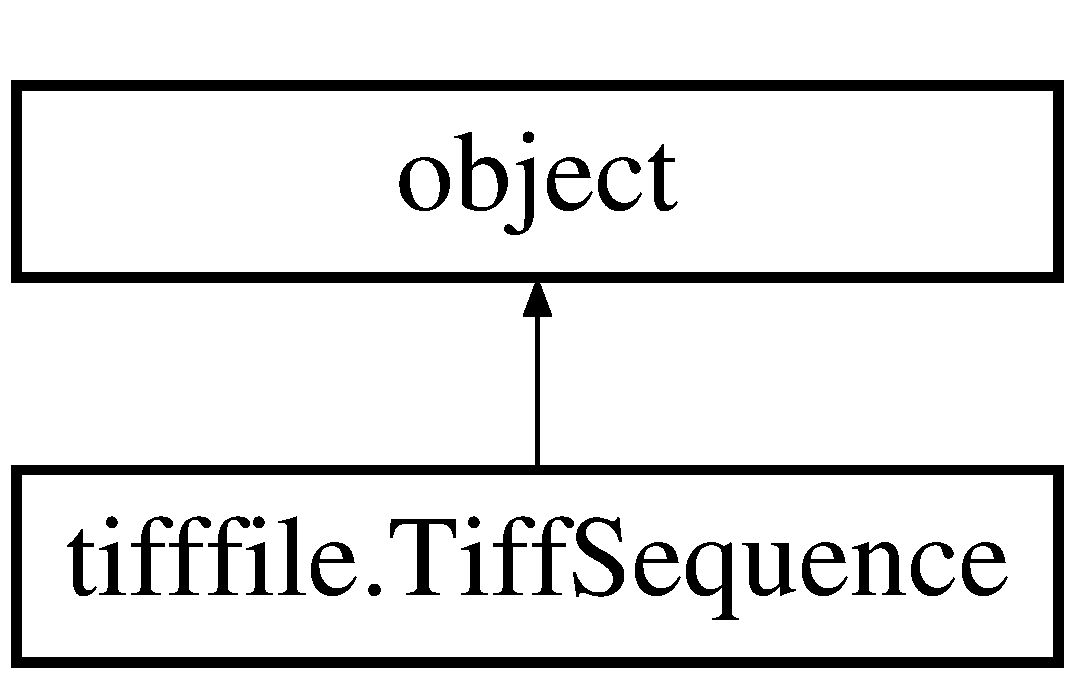
\includegraphics[height=2.000000cm]{classtifffile_1_1_tiff_sequence}
\end{center}
\end{figure}
\subsection*{Classes}
\begin{DoxyCompactItemize}
\item 
class \hyperlink{classtifffile_1_1_tiff_sequence_1_1_parse_error}{Parse\-Error}
\end{DoxyCompactItemize}
\subsection*{Public Member Functions}
\begin{DoxyCompactItemize}
\item 
def \hyperlink{classtifffile_1_1_tiff_sequence_ad2a937998bb0fbb469fd45af3c5b9ee4}{\-\_\-\-\_\-init\-\_\-\-\_\-}
\item 
def \hyperlink{classtifffile_1_1_tiff_sequence_ab271e42b6b0a2d34069c16813b3c6396}{\-\_\-\-\_\-str\-\_\-\-\_\-}
\item 
def \hyperlink{classtifffile_1_1_tiff_sequence_a1e84248e6ff24c50927c27ea3387ae20}{\-\_\-\-\_\-len\-\_\-\-\_\-}
\item 
def \hyperlink{classtifffile_1_1_tiff_sequence_a22f8614649ba8ee39f28db15de453406}{\-\_\-\-\_\-enter\-\_\-\-\_\-}
\item 
def \hyperlink{classtifffile_1_1_tiff_sequence_a5af53397d4d20dc45a6afeafb7798103}{\-\_\-\-\_\-exit\-\_\-\-\_\-}
\item 
def \hyperlink{classtifffile_1_1_tiff_sequence_a66ea3eced1f21205b7fbc4632b7cf41a}{close}
\item 
def \hyperlink{classtifffile_1_1_tiff_sequence_a881cfef0cf4ae0deb1a3fd40b57ff38a}{asarray}
\end{DoxyCompactItemize}
\subsection*{Public Attributes}
\begin{DoxyCompactItemize}
\item 
\hyperlink{classtifffile_1_1_tiff_sequence_a734d6dfdbfbdc2d26c59e7413e9f78d4}{files}
\item 
\hyperlink{classtifffile_1_1_tiff_sequence_a656d87f405cb67c7744470bef749c09d}{imread}
\item 
\hyperlink{classtifffile_1_1_tiff_sequence_a3ced8e56728d8dc84b95cd0e28dd8b29}{pattern}
\item 
\hyperlink{classtifffile_1_1_tiff_sequence_af80218f30eebb11ff3054df126b5e800}{axes}
\item 
\hyperlink{classtifffile_1_1_tiff_sequence_ae581d8715f29b3c6d03df21d139d68c9}{shape}
\end{DoxyCompactItemize}


\subsection{Detailed Description}
\begin{DoxyVerb}Sequence of image files.

The data shape and dtype of all files must match.

Properties
----------
files : list
    List of file names.
shape : tuple
    Shape of image sequence.
axes : str
    Labels of axes in shape.

Examples
--------
>>> tifs = TiffSequence("test.oif.files/*.tif")
>>> tifs.shape, tifs.axes
((2, 100), 'CT')
>>> data = tifs.asarray()
>>> data.shape
(2, 100, 256, 256)\end{DoxyVerb}
 

\subsection{Constructor \& Destructor Documentation}
\hypertarget{classtifffile_1_1_tiff_sequence_ad2a937998bb0fbb469fd45af3c5b9ee4}{\index{tifffile\-::\-Tiff\-Sequence@{tifffile\-::\-Tiff\-Sequence}!\-\_\-\-\_\-init\-\_\-\-\_\-@{\-\_\-\-\_\-init\-\_\-\-\_\-}}
\index{\-\_\-\-\_\-init\-\_\-\-\_\-@{\-\_\-\-\_\-init\-\_\-\-\_\-}!tifffile::TiffSequence@{tifffile\-::\-Tiff\-Sequence}}
\subsubsection[{\-\_\-\-\_\-init\-\_\-\-\_\-}]{\setlength{\rightskip}{0pt plus 5cm}def tifffile.\-Tiff\-Sequence.\-\_\-\-\_\-init\-\_\-\-\_\- (
\begin{DoxyParamCaption}
\item[{}]{self, }
\item[{}]{files, }
\item[{}]{imread = {\ttfamily {\bf Tiff\-File}}, }
\item[{}]{pattern = {\ttfamily '{\bf axes}'}, }
\item[{}]{args, }
\item[{}]{kwargs}
\end{DoxyParamCaption}
)}}\label{classtifffile_1_1_tiff_sequence_ad2a937998bb0fbb469fd45af3c5b9ee4}
\begin{DoxyVerb}Initialize instance from multiple files.

Parameters
----------
files : str, or sequence of str
    Glob pattern or sequence of file names.
imread : function or class
    Image read function or class with asarray function returning numpy
    array from single file.
pattern : str
    Regular expression pattern that matches axes names and sequence
    indices in file names.
    By default this matches Olympus OIF and Leica TIFF series.\end{DoxyVerb}
 

\subsection{Member Function Documentation}
\hypertarget{classtifffile_1_1_tiff_sequence_a22f8614649ba8ee39f28db15de453406}{\index{tifffile\-::\-Tiff\-Sequence@{tifffile\-::\-Tiff\-Sequence}!\-\_\-\-\_\-enter\-\_\-\-\_\-@{\-\_\-\-\_\-enter\-\_\-\-\_\-}}
\index{\-\_\-\-\_\-enter\-\_\-\-\_\-@{\-\_\-\-\_\-enter\-\_\-\-\_\-}!tifffile::TiffSequence@{tifffile\-::\-Tiff\-Sequence}}
\subsubsection[{\-\_\-\-\_\-enter\-\_\-\-\_\-}]{\setlength{\rightskip}{0pt plus 5cm}def tifffile.\-Tiff\-Sequence.\-\_\-\-\_\-enter\-\_\-\-\_\- (
\begin{DoxyParamCaption}
\item[{}]{self}
\end{DoxyParamCaption}
)}}\label{classtifffile_1_1_tiff_sequence_a22f8614649ba8ee39f28db15de453406}
\hypertarget{classtifffile_1_1_tiff_sequence_a5af53397d4d20dc45a6afeafb7798103}{\index{tifffile\-::\-Tiff\-Sequence@{tifffile\-::\-Tiff\-Sequence}!\-\_\-\-\_\-exit\-\_\-\-\_\-@{\-\_\-\-\_\-exit\-\_\-\-\_\-}}
\index{\-\_\-\-\_\-exit\-\_\-\-\_\-@{\-\_\-\-\_\-exit\-\_\-\-\_\-}!tifffile::TiffSequence@{tifffile\-::\-Tiff\-Sequence}}
\subsubsection[{\-\_\-\-\_\-exit\-\_\-\-\_\-}]{\setlength{\rightskip}{0pt plus 5cm}def tifffile.\-Tiff\-Sequence.\-\_\-\-\_\-exit\-\_\-\-\_\- (
\begin{DoxyParamCaption}
\item[{}]{self, }
\item[{}]{exc\-\_\-type, }
\item[{}]{exc\-\_\-value, }
\item[{}]{traceback}
\end{DoxyParamCaption}
)}}\label{classtifffile_1_1_tiff_sequence_a5af53397d4d20dc45a6afeafb7798103}
\hypertarget{classtifffile_1_1_tiff_sequence_a1e84248e6ff24c50927c27ea3387ae20}{\index{tifffile\-::\-Tiff\-Sequence@{tifffile\-::\-Tiff\-Sequence}!\-\_\-\-\_\-len\-\_\-\-\_\-@{\-\_\-\-\_\-len\-\_\-\-\_\-}}
\index{\-\_\-\-\_\-len\-\_\-\-\_\-@{\-\_\-\-\_\-len\-\_\-\-\_\-}!tifffile::TiffSequence@{tifffile\-::\-Tiff\-Sequence}}
\subsubsection[{\-\_\-\-\_\-len\-\_\-\-\_\-}]{\setlength{\rightskip}{0pt plus 5cm}def tifffile.\-Tiff\-Sequence.\-\_\-\-\_\-len\-\_\-\-\_\- (
\begin{DoxyParamCaption}
\item[{}]{self}
\end{DoxyParamCaption}
)}}\label{classtifffile_1_1_tiff_sequence_a1e84248e6ff24c50927c27ea3387ae20}
\hypertarget{classtifffile_1_1_tiff_sequence_ab271e42b6b0a2d34069c16813b3c6396}{\index{tifffile\-::\-Tiff\-Sequence@{tifffile\-::\-Tiff\-Sequence}!\-\_\-\-\_\-str\-\_\-\-\_\-@{\-\_\-\-\_\-str\-\_\-\-\_\-}}
\index{\-\_\-\-\_\-str\-\_\-\-\_\-@{\-\_\-\-\_\-str\-\_\-\-\_\-}!tifffile::TiffSequence@{tifffile\-::\-Tiff\-Sequence}}
\subsubsection[{\-\_\-\-\_\-str\-\_\-\-\_\-}]{\setlength{\rightskip}{0pt plus 5cm}def tifffile.\-Tiff\-Sequence.\-\_\-\-\_\-str\-\_\-\-\_\- (
\begin{DoxyParamCaption}
\item[{}]{self}
\end{DoxyParamCaption}
)}}\label{classtifffile_1_1_tiff_sequence_ab271e42b6b0a2d34069c16813b3c6396}
\begin{DoxyVerb}Return string with information about image sequence.\end{DoxyVerb}
 \hypertarget{classtifffile_1_1_tiff_sequence_a881cfef0cf4ae0deb1a3fd40b57ff38a}{\index{tifffile\-::\-Tiff\-Sequence@{tifffile\-::\-Tiff\-Sequence}!asarray@{asarray}}
\index{asarray@{asarray}!tifffile::TiffSequence@{tifffile\-::\-Tiff\-Sequence}}
\subsubsection[{asarray}]{\setlength{\rightskip}{0pt plus 5cm}def tifffile.\-Tiff\-Sequence.\-asarray (
\begin{DoxyParamCaption}
\item[{}]{self, }
\item[{}]{memmap = {\ttfamily False}, }
\item[{}]{args, }
\item[{}]{kwargs}
\end{DoxyParamCaption}
)}}\label{classtifffile_1_1_tiff_sequence_a881cfef0cf4ae0deb1a3fd40b57ff38a}
\begin{DoxyVerb}Read image data from all files and return as single numpy array.

If memmap is True, return an array stored in a binary file on disk.
The args and kwargs parameters are passed to the imread function.

Raise IndexError or ValueError if image shapes don't match.\end{DoxyVerb}
 \hypertarget{classtifffile_1_1_tiff_sequence_a66ea3eced1f21205b7fbc4632b7cf41a}{\index{tifffile\-::\-Tiff\-Sequence@{tifffile\-::\-Tiff\-Sequence}!close@{close}}
\index{close@{close}!tifffile::TiffSequence@{tifffile\-::\-Tiff\-Sequence}}
\subsubsection[{close}]{\setlength{\rightskip}{0pt plus 5cm}def tifffile.\-Tiff\-Sequence.\-close (
\begin{DoxyParamCaption}
\item[{}]{self}
\end{DoxyParamCaption}
)}}\label{classtifffile_1_1_tiff_sequence_a66ea3eced1f21205b7fbc4632b7cf41a}


\subsection{Member Data Documentation}
\hypertarget{classtifffile_1_1_tiff_sequence_af80218f30eebb11ff3054df126b5e800}{\index{tifffile\-::\-Tiff\-Sequence@{tifffile\-::\-Tiff\-Sequence}!axes@{axes}}
\index{axes@{axes}!tifffile::TiffSequence@{tifffile\-::\-Tiff\-Sequence}}
\subsubsection[{axes}]{\setlength{\rightskip}{0pt plus 5cm}tifffile.\-Tiff\-Sequence.\-axes}}\label{classtifffile_1_1_tiff_sequence_af80218f30eebb11ff3054df126b5e800}
\hypertarget{classtifffile_1_1_tiff_sequence_a734d6dfdbfbdc2d26c59e7413e9f78d4}{\index{tifffile\-::\-Tiff\-Sequence@{tifffile\-::\-Tiff\-Sequence}!files@{files}}
\index{files@{files}!tifffile::TiffSequence@{tifffile\-::\-Tiff\-Sequence}}
\subsubsection[{files}]{\setlength{\rightskip}{0pt plus 5cm}tifffile.\-Tiff\-Sequence.\-files}}\label{classtifffile_1_1_tiff_sequence_a734d6dfdbfbdc2d26c59e7413e9f78d4}
\hypertarget{classtifffile_1_1_tiff_sequence_a656d87f405cb67c7744470bef749c09d}{\index{tifffile\-::\-Tiff\-Sequence@{tifffile\-::\-Tiff\-Sequence}!imread@{imread}}
\index{imread@{imread}!tifffile::TiffSequence@{tifffile\-::\-Tiff\-Sequence}}
\subsubsection[{imread}]{\setlength{\rightskip}{0pt plus 5cm}tifffile.\-Tiff\-Sequence.\-imread}}\label{classtifffile_1_1_tiff_sequence_a656d87f405cb67c7744470bef749c09d}
\hypertarget{classtifffile_1_1_tiff_sequence_a3ced8e56728d8dc84b95cd0e28dd8b29}{\index{tifffile\-::\-Tiff\-Sequence@{tifffile\-::\-Tiff\-Sequence}!pattern@{pattern}}
\index{pattern@{pattern}!tifffile::TiffSequence@{tifffile\-::\-Tiff\-Sequence}}
\subsubsection[{pattern}]{\setlength{\rightskip}{0pt plus 5cm}tifffile.\-Tiff\-Sequence.\-pattern}}\label{classtifffile_1_1_tiff_sequence_a3ced8e56728d8dc84b95cd0e28dd8b29}
\hypertarget{classtifffile_1_1_tiff_sequence_ae581d8715f29b3c6d03df21d139d68c9}{\index{tifffile\-::\-Tiff\-Sequence@{tifffile\-::\-Tiff\-Sequence}!shape@{shape}}
\index{shape@{shape}!tifffile::TiffSequence@{tifffile\-::\-Tiff\-Sequence}}
\subsubsection[{shape}]{\setlength{\rightskip}{0pt plus 5cm}tifffile.\-Tiff\-Sequence.\-shape}}\label{classtifffile_1_1_tiff_sequence_ae581d8715f29b3c6d03df21d139d68c9}


The documentation for this class was generated from the following file\-:\begin{DoxyCompactItemize}
\item 
workdir/atrex/\-Software/\hyperlink{tifffile_8py}{tifffile.\-py}\end{DoxyCompactItemize}

\hypertarget{classtifffile_1_1_tiff_tag}{\section{tifffile.\-Tiff\-Tag Class Reference}
\label{classtifffile_1_1_tiff_tag}\index{tifffile.\-Tiff\-Tag@{tifffile.\-Tiff\-Tag}}
}
Inheritance diagram for tifffile.\-Tiff\-Tag\-:\begin{figure}[H]
\begin{center}
\leavevmode
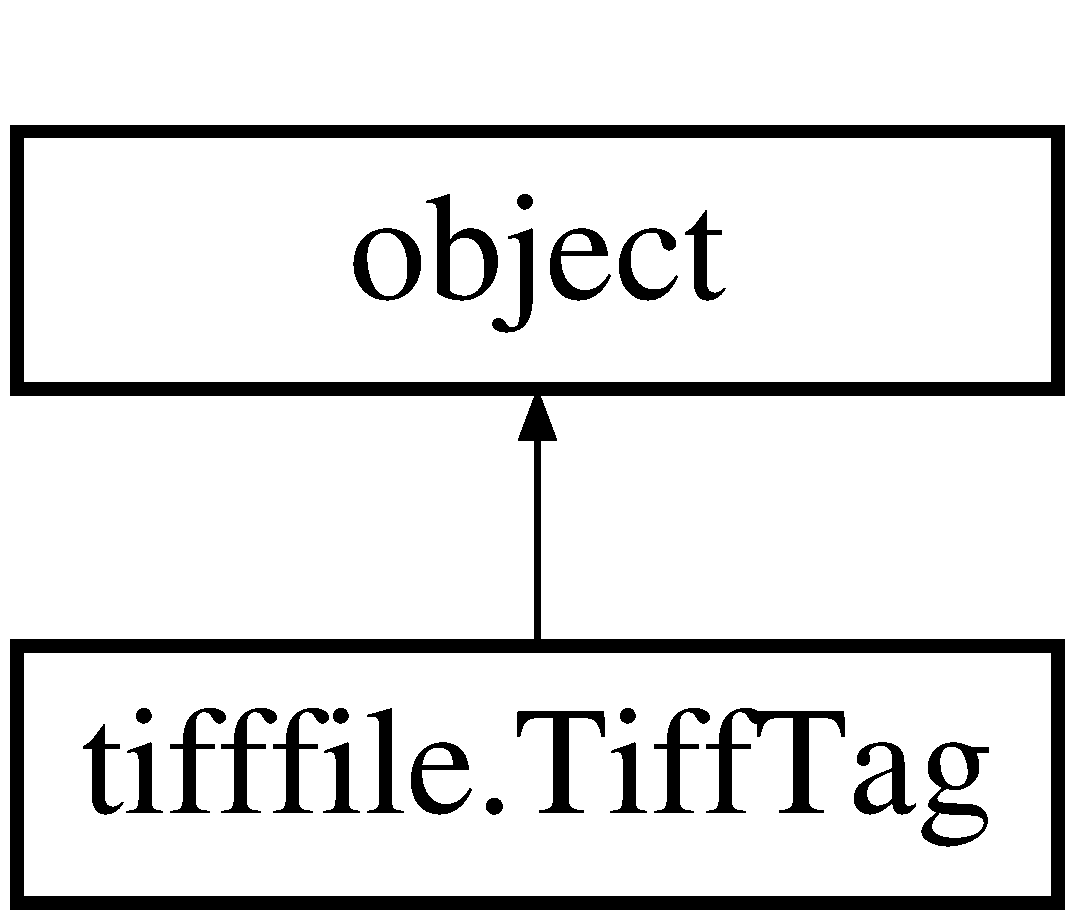
\includegraphics[height=2.000000cm]{classtifffile_1_1_tiff_tag}
\end{center}
\end{figure}
\subsection*{Classes}
\begin{DoxyCompactItemize}
\item 
class \hyperlink{classtifffile_1_1_tiff_tag_1_1_error}{Error}
\end{DoxyCompactItemize}
\subsection*{Public Member Functions}
\begin{DoxyCompactItemize}
\item 
def \hyperlink{classtifffile_1_1_tiff_tag_ace152e86d4dec367306b2aa8c966870a}{\-\_\-\-\_\-init\-\_\-\-\_\-}
\item 
def \hyperlink{classtifffile_1_1_tiff_tag_a6ee3a148b9b7d1233b30a011c0bbcecf}{as\-\_\-str}
\item 
def \hyperlink{classtifffile_1_1_tiff_tag_a3566254292688e9a17f1d71e1506c025}{\-\_\-\-\_\-str\-\_\-\-\_\-}
\end{DoxyCompactItemize}
\subsection*{Public Attributes}
\begin{DoxyCompactItemize}
\item 
\hyperlink{classtifffile_1_1_tiff_tag_a361450aec8540d6ae10e09a51cdd9bee}{code}
\item 
\hyperlink{classtifffile_1_1_tiff_tag_ac34a7b79c29ce864523c939668c5e4f7}{name}
\item 
\hyperlink{classtifffile_1_1_tiff_tag_a31e69f1557e2a9799fdddd2d461c4776}{dtype}
\item 
\hyperlink{classtifffile_1_1_tiff_tag_a20b7fd8e18b9c23e1e55a9bbdc00da3c}{count}
\item 
\hyperlink{classtifffile_1_1_tiff_tag_a0578d5c23f06bde73d1728eb8da3461b}{value}
\item 
\hyperlink{classtifffile_1_1_tiff_tag_ac86aee4a1ef18fc194e4f0c753f74002}{value\-\_\-offset}
\end{DoxyCompactItemize}


\subsection{Detailed Description}
\begin{DoxyVerb}A TIFF tag structure.

Attributes
----------
name : string
    Attribute name of tag.
code : int
    Decimal code of tag.
dtype : str
    Datatype of tag data. One of TIFF_DATA_TYPES.
count : int
    Number of values.
value : various types
    Tag data as Python object.
value_offset : int
    Location of value in file, if any.

All attributes are read-only.\end{DoxyVerb}
 

\subsection{Constructor \& Destructor Documentation}
\hypertarget{classtifffile_1_1_tiff_tag_ace152e86d4dec367306b2aa8c966870a}{\index{tifffile\-::\-Tiff\-Tag@{tifffile\-::\-Tiff\-Tag}!\-\_\-\-\_\-init\-\_\-\-\_\-@{\-\_\-\-\_\-init\-\_\-\-\_\-}}
\index{\-\_\-\-\_\-init\-\_\-\-\_\-@{\-\_\-\-\_\-init\-\_\-\-\_\-}!tifffile::TiffTag@{tifffile\-::\-Tiff\-Tag}}
\subsubsection[{\-\_\-\-\_\-init\-\_\-\-\_\-}]{\setlength{\rightskip}{0pt plus 5cm}def tifffile.\-Tiff\-Tag.\-\_\-\-\_\-init\-\_\-\-\_\- (
\begin{DoxyParamCaption}
\item[{}]{self, }
\item[{}]{arg, }
\item[{}]{kwargs}
\end{DoxyParamCaption}
)}}\label{classtifffile_1_1_tiff_tag_ace152e86d4dec367306b2aa8c966870a}
\begin{DoxyVerb}Initialize instance from file or arguments.\end{DoxyVerb}
 

\subsection{Member Function Documentation}
\hypertarget{classtifffile_1_1_tiff_tag_a3566254292688e9a17f1d71e1506c025}{\index{tifffile\-::\-Tiff\-Tag@{tifffile\-::\-Tiff\-Tag}!\-\_\-\-\_\-str\-\_\-\-\_\-@{\-\_\-\-\_\-str\-\_\-\-\_\-}}
\index{\-\_\-\-\_\-str\-\_\-\-\_\-@{\-\_\-\-\_\-str\-\_\-\-\_\-}!tifffile::TiffTag@{tifffile\-::\-Tiff\-Tag}}
\subsubsection[{\-\_\-\-\_\-str\-\_\-\-\_\-}]{\setlength{\rightskip}{0pt plus 5cm}def tifffile.\-Tiff\-Tag.\-\_\-\-\_\-str\-\_\-\-\_\- (
\begin{DoxyParamCaption}
\item[{}]{self}
\end{DoxyParamCaption}
)}}\label{classtifffile_1_1_tiff_tag_a3566254292688e9a17f1d71e1506c025}
\begin{DoxyVerb}Return string containing information about tag.\end{DoxyVerb}
 \hypertarget{classtifffile_1_1_tiff_tag_a6ee3a148b9b7d1233b30a011c0bbcecf}{\index{tifffile\-::\-Tiff\-Tag@{tifffile\-::\-Tiff\-Tag}!as\-\_\-str@{as\-\_\-str}}
\index{as\-\_\-str@{as\-\_\-str}!tifffile::TiffTag@{tifffile\-::\-Tiff\-Tag}}
\subsubsection[{as\-\_\-str}]{\setlength{\rightskip}{0pt plus 5cm}def tifffile.\-Tiff\-Tag.\-as\-\_\-str (
\begin{DoxyParamCaption}
\item[{}]{self}
\end{DoxyParamCaption}
)}}\label{classtifffile_1_1_tiff_tag_a6ee3a148b9b7d1233b30a011c0bbcecf}
\begin{DoxyVerb}Return value as human readable string.\end{DoxyVerb}
 

\subsection{Member Data Documentation}
\hypertarget{classtifffile_1_1_tiff_tag_a361450aec8540d6ae10e09a51cdd9bee}{\index{tifffile\-::\-Tiff\-Tag@{tifffile\-::\-Tiff\-Tag}!code@{code}}
\index{code@{code}!tifffile::TiffTag@{tifffile\-::\-Tiff\-Tag}}
\subsubsection[{code}]{\setlength{\rightskip}{0pt plus 5cm}tifffile.\-Tiff\-Tag.\-code}}\label{classtifffile_1_1_tiff_tag_a361450aec8540d6ae10e09a51cdd9bee}
\hypertarget{classtifffile_1_1_tiff_tag_a20b7fd8e18b9c23e1e55a9bbdc00da3c}{\index{tifffile\-::\-Tiff\-Tag@{tifffile\-::\-Tiff\-Tag}!count@{count}}
\index{count@{count}!tifffile::TiffTag@{tifffile\-::\-Tiff\-Tag}}
\subsubsection[{count}]{\setlength{\rightskip}{0pt plus 5cm}tifffile.\-Tiff\-Tag.\-count}}\label{classtifffile_1_1_tiff_tag_a20b7fd8e18b9c23e1e55a9bbdc00da3c}
\hypertarget{classtifffile_1_1_tiff_tag_a31e69f1557e2a9799fdddd2d461c4776}{\index{tifffile\-::\-Tiff\-Tag@{tifffile\-::\-Tiff\-Tag}!dtype@{dtype}}
\index{dtype@{dtype}!tifffile::TiffTag@{tifffile\-::\-Tiff\-Tag}}
\subsubsection[{dtype}]{\setlength{\rightskip}{0pt plus 5cm}tifffile.\-Tiff\-Tag.\-dtype}}\label{classtifffile_1_1_tiff_tag_a31e69f1557e2a9799fdddd2d461c4776}
\hypertarget{classtifffile_1_1_tiff_tag_ac34a7b79c29ce864523c939668c5e4f7}{\index{tifffile\-::\-Tiff\-Tag@{tifffile\-::\-Tiff\-Tag}!name@{name}}
\index{name@{name}!tifffile::TiffTag@{tifffile\-::\-Tiff\-Tag}}
\subsubsection[{name}]{\setlength{\rightskip}{0pt plus 5cm}tifffile.\-Tiff\-Tag.\-name}}\label{classtifffile_1_1_tiff_tag_ac34a7b79c29ce864523c939668c5e4f7}
\hypertarget{classtifffile_1_1_tiff_tag_a0578d5c23f06bde73d1728eb8da3461b}{\index{tifffile\-::\-Tiff\-Tag@{tifffile\-::\-Tiff\-Tag}!value@{value}}
\index{value@{value}!tifffile::TiffTag@{tifffile\-::\-Tiff\-Tag}}
\subsubsection[{value}]{\setlength{\rightskip}{0pt plus 5cm}tifffile.\-Tiff\-Tag.\-value}}\label{classtifffile_1_1_tiff_tag_a0578d5c23f06bde73d1728eb8da3461b}
\hypertarget{classtifffile_1_1_tiff_tag_ac86aee4a1ef18fc194e4f0c753f74002}{\index{tifffile\-::\-Tiff\-Tag@{tifffile\-::\-Tiff\-Tag}!value\-\_\-offset@{value\-\_\-offset}}
\index{value\-\_\-offset@{value\-\_\-offset}!tifffile::TiffTag@{tifffile\-::\-Tiff\-Tag}}
\subsubsection[{value\-\_\-offset}]{\setlength{\rightskip}{0pt plus 5cm}tifffile.\-Tiff\-Tag.\-value\-\_\-offset}}\label{classtifffile_1_1_tiff_tag_ac86aee4a1ef18fc194e4f0c753f74002}


The documentation for this class was generated from the following file\-:\begin{DoxyCompactItemize}
\item 
workdir/atrex/\-Software/\hyperlink{tifffile_8py}{tifffile.\-py}\end{DoxyCompactItemize}

\hypertarget{classtifffile_1_1_tiff_tags}{\section{tifffile.\-Tiff\-Tags Class Reference}
\label{classtifffile_1_1_tiff_tags}\index{tifffile.\-Tiff\-Tags@{tifffile.\-Tiff\-Tags}}
}
Inheritance diagram for tifffile.\-Tiff\-Tags\-:\begin{figure}[H]
\begin{center}
\leavevmode
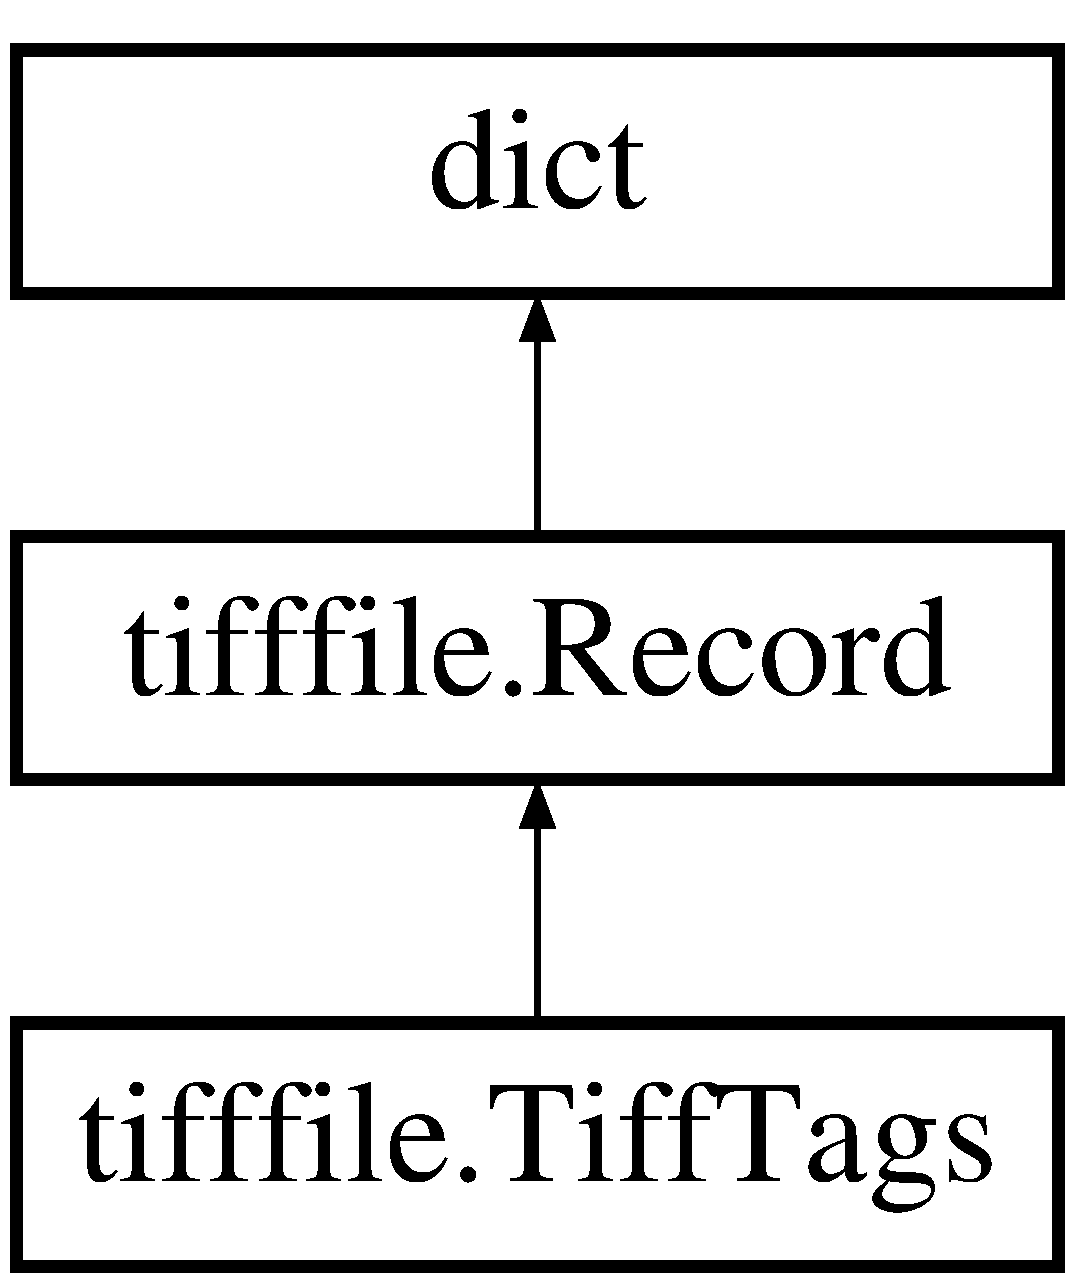
\includegraphics[height=3.000000cm]{classtifffile_1_1_tiff_tags}
\end{center}
\end{figure}
\subsection*{Public Member Functions}
\begin{DoxyCompactItemize}
\item 
def \hyperlink{classtifffile_1_1_tiff_tags_a68afbd2339eb5c7a6c02eea60a16ce65}{\-\_\-\-\_\-str\-\_\-\-\_\-}
\end{DoxyCompactItemize}


\subsection{Detailed Description}
\begin{DoxyVerb}Dictionary of TiffTag with attribute access.\end{DoxyVerb}
 

\subsection{Member Function Documentation}
\hypertarget{classtifffile_1_1_tiff_tags_a68afbd2339eb5c7a6c02eea60a16ce65}{\index{tifffile\-::\-Tiff\-Tags@{tifffile\-::\-Tiff\-Tags}!\-\_\-\-\_\-str\-\_\-\-\_\-@{\-\_\-\-\_\-str\-\_\-\-\_\-}}
\index{\-\_\-\-\_\-str\-\_\-\-\_\-@{\-\_\-\-\_\-str\-\_\-\-\_\-}!tifffile::TiffTags@{tifffile\-::\-Tiff\-Tags}}
\subsubsection[{\-\_\-\-\_\-str\-\_\-\-\_\-}]{\setlength{\rightskip}{0pt plus 5cm}def tifffile.\-Tiff\-Tags.\-\_\-\-\_\-str\-\_\-\-\_\- (
\begin{DoxyParamCaption}
\item[{}]{self}
\end{DoxyParamCaption}
)}}\label{classtifffile_1_1_tiff_tags_a68afbd2339eb5c7a6c02eea60a16ce65}
\begin{DoxyVerb}Return string with information about all tags.\end{DoxyVerb}
 

The documentation for this class was generated from the following file\-:\begin{DoxyCompactItemize}
\item 
workdir/atrex/\-Software/\hyperlink{tifffile_8py}{tifffile.\-py}\end{DoxyCompactItemize}

\hypertarget{classtifffile_1_1_tiff_writer}{\section{tifffile.\-Tiff\-Writer Class Reference}
\label{classtifffile_1_1_tiff_writer}\index{tifffile.\-Tiff\-Writer@{tifffile.\-Tiff\-Writer}}
}
Inheritance diagram for tifffile.\-Tiff\-Writer\-:\begin{figure}[H]
\begin{center}
\leavevmode
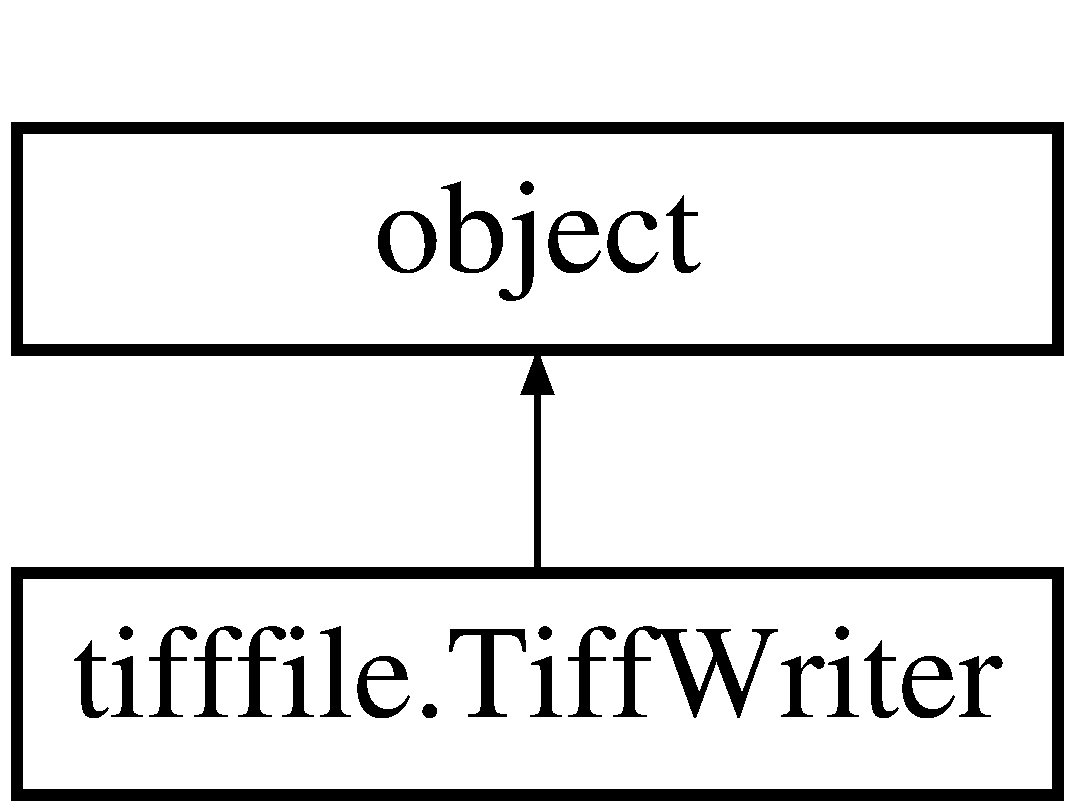
\includegraphics[height=2.000000cm]{classtifffile_1_1_tiff_writer}
\end{center}
\end{figure}
\subsection*{Public Member Functions}
\begin{DoxyCompactItemize}
\item 
def \hyperlink{classtifffile_1_1_tiff_writer_af9fb37461e229375ed0b7c7aa56fcf2a}{\-\_\-\-\_\-init\-\_\-\-\_\-}
\item 
def \hyperlink{classtifffile_1_1_tiff_writer_a7879708dbcc972bda2148374bddbec0d}{save}
\item 
def \hyperlink{classtifffile_1_1_tiff_writer_a579dd794187e65874987990058ba70aa}{close}
\item 
def \hyperlink{classtifffile_1_1_tiff_writer_aeb1a99b0e609acf41b4a96029397724d}{\-\_\-\-\_\-enter\-\_\-\-\_\-}
\item 
def \hyperlink{classtifffile_1_1_tiff_writer_a9a746e2cea3adaab40913a74fb56ca60}{\-\_\-\-\_\-exit\-\_\-\-\_\-}
\end{DoxyCompactItemize}
\subsection*{Static Public Attributes}
\begin{DoxyCompactItemize}
\item 
dictionary \hyperlink{classtifffile_1_1_tiff_writer_aae9c1bc9345c95fe80d2d31188e6e23d}{T\-Y\-P\-E\-S}
\item 
dictionary \hyperlink{classtifffile_1_1_tiff_writer_a59306b1d4123917f8ef19b622932be69}{T\-A\-G\-S}
\end{DoxyCompactItemize}


\subsection{Detailed Description}
\begin{DoxyVerb}Write image data to TIFF file.

TiffWriter instances must be closed using the close method, which is
automatically called when using the 'with' statement.

Examples
--------
>>> data = numpy.random.rand(2, 5, 3, 301, 219)
>>> with TiffWriter('temp.tif', bigtiff=True) as tif:
...     for i in range(data.shape[0]):
...         tif.save(data[i], compress=6)\end{DoxyVerb}
 

\subsection{Constructor \& Destructor Documentation}
\hypertarget{classtifffile_1_1_tiff_writer_af9fb37461e229375ed0b7c7aa56fcf2a}{\index{tifffile\-::\-Tiff\-Writer@{tifffile\-::\-Tiff\-Writer}!\-\_\-\-\_\-init\-\_\-\-\_\-@{\-\_\-\-\_\-init\-\_\-\-\_\-}}
\index{\-\_\-\-\_\-init\-\_\-\-\_\-@{\-\_\-\-\_\-init\-\_\-\-\_\-}!tifffile::TiffWriter@{tifffile\-::\-Tiff\-Writer}}
\subsubsection[{\-\_\-\-\_\-init\-\_\-\-\_\-}]{\setlength{\rightskip}{0pt plus 5cm}def tifffile.\-Tiff\-Writer.\-\_\-\-\_\-init\-\_\-\-\_\- (
\begin{DoxyParamCaption}
\item[{}]{self, }
\item[{}]{filename, }
\item[{}]{bigtiff = {\ttfamily False}, }
\item[{}]{byteorder = {\ttfamily None}, }
\item[{}]{software = {\ttfamily 'tifffile.py'}}
\end{DoxyParamCaption}
)}}\label{classtifffile_1_1_tiff_writer_af9fb37461e229375ed0b7c7aa56fcf2a}
\begin{DoxyVerb}Create a new TIFF file for writing.

Use bigtiff=True when creating files greater than 2 GB.

Parameters
----------
filename : str
    Name of file to write.
bigtiff : bool
    If True, the BigTIFF format is used.
byteorder : {'<', '>'}
    The endianness of the data in the file.
    By default this is the system's native byte order.
software : str
    Name of the software used to create the image.
    Saved with the first page only.\end{DoxyVerb}
 

\subsection{Member Function Documentation}
\hypertarget{classtifffile_1_1_tiff_writer_aeb1a99b0e609acf41b4a96029397724d}{\index{tifffile\-::\-Tiff\-Writer@{tifffile\-::\-Tiff\-Writer}!\-\_\-\-\_\-enter\-\_\-\-\_\-@{\-\_\-\-\_\-enter\-\_\-\-\_\-}}
\index{\-\_\-\-\_\-enter\-\_\-\-\_\-@{\-\_\-\-\_\-enter\-\_\-\-\_\-}!tifffile::TiffWriter@{tifffile\-::\-Tiff\-Writer}}
\subsubsection[{\-\_\-\-\_\-enter\-\_\-\-\_\-}]{\setlength{\rightskip}{0pt plus 5cm}def tifffile.\-Tiff\-Writer.\-\_\-\-\_\-enter\-\_\-\-\_\- (
\begin{DoxyParamCaption}
\item[{}]{self}
\end{DoxyParamCaption}
)}}\label{classtifffile_1_1_tiff_writer_aeb1a99b0e609acf41b4a96029397724d}
\hypertarget{classtifffile_1_1_tiff_writer_a9a746e2cea3adaab40913a74fb56ca60}{\index{tifffile\-::\-Tiff\-Writer@{tifffile\-::\-Tiff\-Writer}!\-\_\-\-\_\-exit\-\_\-\-\_\-@{\-\_\-\-\_\-exit\-\_\-\-\_\-}}
\index{\-\_\-\-\_\-exit\-\_\-\-\_\-@{\-\_\-\-\_\-exit\-\_\-\-\_\-}!tifffile::TiffWriter@{tifffile\-::\-Tiff\-Writer}}
\subsubsection[{\-\_\-\-\_\-exit\-\_\-\-\_\-}]{\setlength{\rightskip}{0pt plus 5cm}def tifffile.\-Tiff\-Writer.\-\_\-\-\_\-exit\-\_\-\-\_\- (
\begin{DoxyParamCaption}
\item[{}]{self, }
\item[{}]{exc\-\_\-type, }
\item[{}]{exc\-\_\-value, }
\item[{}]{traceback}
\end{DoxyParamCaption}
)}}\label{classtifffile_1_1_tiff_writer_a9a746e2cea3adaab40913a74fb56ca60}
\hypertarget{classtifffile_1_1_tiff_writer_a579dd794187e65874987990058ba70aa}{\index{tifffile\-::\-Tiff\-Writer@{tifffile\-::\-Tiff\-Writer}!close@{close}}
\index{close@{close}!tifffile::TiffWriter@{tifffile\-::\-Tiff\-Writer}}
\subsubsection[{close}]{\setlength{\rightskip}{0pt plus 5cm}def tifffile.\-Tiff\-Writer.\-close (
\begin{DoxyParamCaption}
\item[{}]{self}
\end{DoxyParamCaption}
)}}\label{classtifffile_1_1_tiff_writer_a579dd794187e65874987990058ba70aa}
\hypertarget{classtifffile_1_1_tiff_writer_a7879708dbcc972bda2148374bddbec0d}{\index{tifffile\-::\-Tiff\-Writer@{tifffile\-::\-Tiff\-Writer}!save@{save}}
\index{save@{save}!tifffile::TiffWriter@{tifffile\-::\-Tiff\-Writer}}
\subsubsection[{save}]{\setlength{\rightskip}{0pt plus 5cm}def tifffile.\-Tiff\-Writer.\-save (
\begin{DoxyParamCaption}
\item[{}]{self, }
\item[{}]{data, }
\item[{}]{photometric = {\ttfamily None}, }
\item[{}]{planarconfig = {\ttfamily None}, }
\item[{}]{resolution = {\ttfamily None}, }
\item[{}]{description = {\ttfamily None}, }
\item[{}]{volume = {\ttfamily False}, }
\item[{}]{writeshape = {\ttfamily False}, }
\item[{}]{compress = {\ttfamily 0}, }
\item[{}]{extratags = {\ttfamily ()}}
\end{DoxyParamCaption}
)}}\label{classtifffile_1_1_tiff_writer_a7879708dbcc972bda2148374bddbec0d}
\begin{DoxyVerb}Write image data to TIFF file.

Image data are written in one stripe per plane.
Dimensions larger than 2 to 4 (depending on photometric mode, planar
configuration, and SGI mode) are flattened and saved as separate pages.
The 'sample_format' and 'bits_per_sample' TIFF tags are derived from
the data type.

Parameters
----------
data : array_like
    Input image. The last dimensions are assumed to be image depth,
    height, width, and samples.
photometric : {'minisblack', 'miniswhite', 'rgb'}
    The color space of the image data.
    By default this setting is inferred from the data shape.
planarconfig : {'contig', 'planar'}
    Specifies if samples are stored contiguous or in separate planes.
    By default this setting is inferred from the data shape.
    'contig': last dimension contains samples.
    'planar': third last dimension contains samples.
resolution : (float, float) or ((int, int), (int, int))
    X and Y resolution in dots per inch as float or rational numbers.
description : str
    The subject of the image. Saved with the first page only.
compress : int
    Values from 0 to 9 controlling the level of zlib compression.
    If 0, data are written uncompressed (default).
volume : bool
    If True, volume data are stored in one tile (if applicable) using
    the SGI image_depth and tile_depth tags.
    Image width and depth must be multiple of 16.
    Few software can read this format, e.g. MeVisLab.
writeshape : bool
    If True, write the data shape to the image_description tag
    if necessary and no other description is given.
extratags: sequence of tuples
    Additional tags as [(code, dtype, count, value, writeonce)].

    code : int
The TIFF tag Id.
    dtype : str
Data type of items in 'value' in Python struct format.
One of B, s, H, I, 2I, b, h, i, f, d, Q, or q.
    count : int
Number of data values. Not used for string values.
    value : sequence
'Count' values compatible with 'dtype'.
    writeonce : bool
If True, the tag is written to the first page only.\end{DoxyVerb}
 

\subsection{Member Data Documentation}
\hypertarget{classtifffile_1_1_tiff_writer_a59306b1d4123917f8ef19b622932be69}{\index{tifffile\-::\-Tiff\-Writer@{tifffile\-::\-Tiff\-Writer}!T\-A\-G\-S@{T\-A\-G\-S}}
\index{T\-A\-G\-S@{T\-A\-G\-S}!tifffile::TiffWriter@{tifffile\-::\-Tiff\-Writer}}
\subsubsection[{T\-A\-G\-S}]{\setlength{\rightskip}{0pt plus 5cm}dictionary tifffile.\-Tiff\-Writer.\-T\-A\-G\-S\hspace{0.3cm}{\ttfamily [static]}}}\label{classtifffile_1_1_tiff_writer_a59306b1d4123917f8ef19b622932be69}
{\bfseries Initial value\-:}
\begin{DoxyCode}
1 = \{
2         \textcolor{stringliteral}{'new\_subfile\_type'}: 254, \textcolor{stringliteral}{'subfile\_type'}: 255,
3         \textcolor{stringliteral}{'image\_width'}: 256, \textcolor{stringliteral}{'image\_length'}: 257, \textcolor{stringliteral}{'bits\_per\_sample'}: 258,
4         \textcolor{stringliteral}{'compression'}: 259, \textcolor{stringliteral}{'photometric'}: 262, \textcolor{stringliteral}{'fill\_order'}: 266,
5         \textcolor{stringliteral}{'document\_name'}: 269, \textcolor{stringliteral}{'image\_description'}: 270, \textcolor{stringliteral}{'strip\_offsets'}: 273,
6         \textcolor{stringliteral}{'orientation'}: 274, \textcolor{stringliteral}{'samples\_per\_pixel'}: 277, \textcolor{stringliteral}{'rows\_per\_strip'}: 278,
7         \textcolor{stringliteral}{'strip\_byte\_counts'}: 279, \textcolor{stringliteral}{'x\_resolution'}: 282, \textcolor{stringliteral}{'y\_resolution'}: 283,
8         \textcolor{stringliteral}{'planar\_configuration'}: 284, \textcolor{stringliteral}{'page\_name'}: 285, \textcolor{stringliteral}{'resolution\_unit'}: 296,
9         \textcolor{stringliteral}{'software'}: 305, \textcolor{stringliteral}{'datetime'}: 306, \textcolor{stringliteral}{'predictor'}: 317, \textcolor{stringliteral}{'color\_map'}: 320,
10         \textcolor{stringliteral}{'tile\_width'}: 322, \textcolor{stringliteral}{'tile\_length'}: 323, \textcolor{stringliteral}{'tile\_offsets'}: 324,
11         \textcolor{stringliteral}{'tile\_byte\_counts'}: 325, \textcolor{stringliteral}{'extra\_samples'}: 338, \textcolor{stringliteral}{'sample\_format'}: 339,
12         \textcolor{stringliteral}{'image\_depth'}: 32997, \textcolor{stringliteral}{'tile\_depth'}: 32998\}
\end{DoxyCode}
\hypertarget{classtifffile_1_1_tiff_writer_aae9c1bc9345c95fe80d2d31188e6e23d}{\index{tifffile\-::\-Tiff\-Writer@{tifffile\-::\-Tiff\-Writer}!T\-Y\-P\-E\-S@{T\-Y\-P\-E\-S}}
\index{T\-Y\-P\-E\-S@{T\-Y\-P\-E\-S}!tifffile::TiffWriter@{tifffile\-::\-Tiff\-Writer}}
\subsubsection[{T\-Y\-P\-E\-S}]{\setlength{\rightskip}{0pt plus 5cm}dictionary tifffile.\-Tiff\-Writer.\-T\-Y\-P\-E\-S\hspace{0.3cm}{\ttfamily [static]}}}\label{classtifffile_1_1_tiff_writer_aae9c1bc9345c95fe80d2d31188e6e23d}
{\bfseries Initial value\-:}
\begin{DoxyCode}
1 = \{\textcolor{stringliteral}{'B'}: 1, \textcolor{stringliteral}{'s'}: 2, \textcolor{stringliteral}{'H'}: 3, \textcolor{stringliteral}{'I'}: 4, \textcolor{stringliteral}{'2I'}: 5, \textcolor{stringliteral}{'b'}: 6,
2              \textcolor{stringliteral}{'h'}: 8, \textcolor{stringliteral}{'i'}: 9, \textcolor{stringliteral}{'f'}: 11, \textcolor{stringliteral}{'d'}: 12, \textcolor{stringliteral}{'Q'}: 16, \textcolor{stringliteral}{'q'}: 17\}
\end{DoxyCode}


The documentation for this class was generated from the following file\-:\begin{DoxyCompactItemize}
\item 
workdir/atrex/\-Software/\hyperlink{tifffile_8py}{tifffile.\-py}\end{DoxyCompactItemize}

\chapter{File Documentation}
\hypertarget{_atrex_8py}{\section{workdir/atrex/\-Software/\-Atrex.py File Reference}
\label{_atrex_8py}\index{workdir/atrex/\-Software/\-Atrex.\-py@{workdir/atrex/\-Software/\-Atrex.\-py}}
}
\subsection*{Classes}
\begin{DoxyCompactItemize}
\item 
class \hyperlink{class_atrex_1_1_atrex}{Atrex.\-Atrex}
\begin{DoxyCompactList}\small\item\em \hyperlink{class_atrex_1_1_atrex}{Atrex} Top level class of the \hyperlink{class_atrex_1_1_atrex}{Atrex} software package. \end{DoxyCompactList}\end{DoxyCompactItemize}
\subsection*{Namespaces}
\begin{DoxyCompactItemize}
\item 
\hyperlink{namespace_atrex}{Atrex}
\end{DoxyCompactItemize}
\subsection*{Variables}
\begin{DoxyCompactItemize}
\item 
tuple \hyperlink{namespace_atrex_afb58c624b98f7c5df49888bb198f1374}{Atrex.\-app} = Qt\-Gui.\-Q\-Application(sys.\-argv)
\item 
tuple \hyperlink{namespace_atrex_a1af4daf409e7f1e23d2ff5a8352f4da1}{Atrex.\-atrex} = Atrex()
\end{DoxyCompactItemize}

\hypertarget{atrex__utils_8py}{\section{workdir/atrex/\-Software/atrex\-\_\-utils.py File Reference}
\label{atrex__utils_8py}\index{workdir/atrex/\-Software/atrex\-\_\-utils.\-py@{workdir/atrex/\-Software/atrex\-\_\-utils.\-py}}
}
\subsection*{Namespaces}
\begin{DoxyCompactItemize}
\item 
\hyperlink{namespaceatrex__utils}{atrex\-\_\-utils}
\end{DoxyCompactItemize}
\subsection*{Functions}
\begin{DoxyCompactItemize}
\item 
def \hyperlink{namespaceatrex__utils_a9a9c32b8352e0115e6f6c9ab2b8a1b26}{atrex\-\_\-utils.\-my\-Square}
\item 
def \hyperlink{namespaceatrex__utils_a7158daee0e5b25be1fe0a18b082cf86d}{atrex\-\_\-utils.\-get\-Image\-Range}
\end{DoxyCompactItemize}

\hypertarget{congrid_8py}{\section{workdir/atrex/\-Software/congrid.py File Reference}
\label{congrid_8py}\index{workdir/atrex/\-Software/congrid.\-py@{workdir/atrex/\-Software/congrid.\-py}}
}
\subsection*{Namespaces}
\begin{DoxyCompactItemize}
\item 
\hyperlink{namespacecongrid}{congrid}
\end{DoxyCompactItemize}
\subsection*{Functions}
\begin{DoxyCompactItemize}
\item 
def \hyperlink{namespacecongrid_ad23f482f1eb20fb1171adc7f01716d26}{congrid.\-congrid}
\end{DoxyCompactItemize}

\hypertarget{crystallography_8py}{\section{workdir/atrex/\-Software/crystallography.py File Reference}
\label{crystallography_8py}\index{workdir/atrex/\-Software/crystallography.\-py@{workdir/atrex/\-Software/crystallography.\-py}}
}
\subsection*{Namespaces}
\begin{DoxyCompactItemize}
\item 
\hyperlink{namespacecrystallography}{crystallography}
\end{DoxyCompactItemize}
\subsection*{Functions}
\begin{DoxyCompactItemize}
\item 
def \hyperlink{namespacecrystallography_a58171b4824c6f98df0d2200bc258bde2}{crystallography.\-A\-\_\-to\-\_\-kev}
\item 
def \hyperlink{namespacecrystallography_a20e6dff641c1326b0062aabcd924cffd}{crystallography.\-kev\-\_\-to\-\_\-\-A}
\item 
def \hyperlink{namespacecrystallography_ae86fb13e8f363baa1b13639483c01183}{crystallography.\-tth\-\_\-from\-\_\-xyz}
\item 
def \hyperlink{namespacecrystallography_a9efa98c3b1aef1d7beca6fb89086c388}{crystallography.\-en\-\_\-from\-\_\-tth\-\_\-and\-\_\-d}
\item 
def \hyperlink{namespacecrystallography_af940a609cdeb81c339448daa1db7c9a9}{crystallography.\-en\-\_\-from\-\_\-xyz}
\item 
def \hyperlink{namespacecrystallography_a4df51e2fddc4a9c843028a572a645d8a}{crystallography.\-d\-\_\-from\-\_\-tth\-\_\-and\-\_\-en}
\item 
def \hyperlink{namespacecrystallography_aa131e8fb34e0833ceaff1dcdf8337a60}{crystallography.\-tth\-\_\-from\-\_\-en\-\_\-and\-\_\-d}
\item 
def \hyperlink{namespacecrystallography_a797dc74ad0fe257371737f35f5bf44d8}{crystallography.\-tth\-\_\-from\-\_\-hkl\-\_\-and\-\_\-lp}
\item 
def \hyperlink{namespacecrystallography_a5f7e74ec1d11c8cfb020d7ebb515c0c5}{crystallography.\-d\-\_\-from\-\_\-lp\-\_\-and\-\_\-hkl}
\item 
def \hyperlink{namespacecrystallography_a0c041a7a2849ec884fe8bd234b7e04dd}{crystallography.\-equivalent}
\item 
def \hyperlink{namespacecrystallography_a1b5cfcfc56bb0c43e2898b18c2ae0f31}{crystallography.\-b\-\_\-from\-\_\-lp}
\item 
def \hyperlink{namespacecrystallography_a108a8b1c5312871f58ebcbe980b37801}{crystallography.\-dotprod}
\item 
def \hyperlink{namespacecrystallography_aea2c4d89da7b6b57a4d947a51ed67c9e}{crystallography.\-vlength}
\item 
def \hyperlink{namespacecrystallography_aae60d18338e58a21bb9abd24beecbe42}{crystallography.\-ang}
\item 
def \hyperlink{namespacecrystallography_afa94b4aac1d8fd726f31e98915aa3833}{crystallography.\-lp\-\_\-from\-\_\-ub}
\item 
def \hyperlink{namespacecrystallography_a49712413ea299a47440e3db9b0d187cd}{crystallography.\-V\-\_\-from\-\_\-lp}
\item 
def \hyperlink{namespacecrystallography_ace21f698f6a91880ff79b26cce3d44a1}{crystallography.\-V\-\_\-from\-\_\-ub}
\item 
def \hyperlink{namespacecrystallography_a8b7bd586e750f963562e8811b171dc85}{crystallography.\-U\-\_\-from\-\_\-ub}
\item 
def \hyperlink{namespacecrystallography_ade33673c59999578962f7e3574fd66f5}{crystallography.\-hkl\-\_\-from\-\_\-ub\-\_\-and\-\_\-xyz}
\item 
def \hyperlink{namespacecrystallography_a1135eb3d895d4db119f03dfe03b16246}{crystallography.\-find\-\_\-possible\-\_\-hkls}
\item 
def \hyperlink{namespacecrystallography_afc7e18304cb893ba82f482dda7a8203a}{crystallography.\-flags\-\_\-from\-\_\-sym}
\item 
def \hyperlink{namespacecrystallography_a4e57db686b17b444803bf0b345633bcc}{crystallography.\-syst\-\_\-extinction}
\item 
def \hyperlink{namespacecrystallography_a3e5709b266157e0701be4d336c074648}{crystallography.\-apply\-\_\-symmetry\-\_\-to\-\_\-lp}
\item 
def \hyperlink{namespacecrystallography_aceeb721a52e4341dc482f2830ab13c9c}{crystallography.\-angle\-\_\-between\-\_\-hkls}
\item 
def \hyperlink{namespacecrystallography_af905b3d3c9e00d94a3bda5150b55d8bd}{crystallography.\-calc\-\_\-ub\-\_\-from\-\_\-three}
\item 
def \hyperlink{namespacecrystallography_a5c3a3554b9a344670d7ea9126758f76d}{crystallography.\-get\-\_\-omega}
\begin{DoxyCompactList}\small\item\em get\-\_\-omega -- From xyz and energy calculates the omega angle (in deg) at which xyz will come into diffracting position during omega scan at chi 0 if diffraction position inaccessible in omega scan returns \mbox{[}-\/1000,-\/1000\mbox{]} \end{DoxyCompactList}\item 
def \hyperlink{namespacecrystallography_a135f57254d70c8f690eb769d3ad18437}{crystallography.\-general\-\_\-axis}
\item 
def \hyperlink{namespacecrystallography_ada28fca5d9f6fd5ab456edc3e32713e1}{crystallography.\-solve\-\_\-general\-\_\-axis}
\item 
def \hyperlink{namespacecrystallography_a0a424f36ab371104637e16161cbf9b73}{crystallography.\-sincos}
\item 
def \hyperlink{namespacecrystallography_a0da34711a0fdb2fc186eac5a965e35d6}{crystallography.\-open\-\_\-\-U\-B}
\end{DoxyCompactItemize}
\subsection*{Variables}
\begin{DoxyCompactItemize}
\item 
int \hyperlink{namespacecrystallography_ad28d74622030c2011af7636d2657ed99}{crystallography.\-D\-T\-O\-R} = math.\-pi/180
\item 
int \hyperlink{namespacecrystallography_ad0848788e86c4a194771f24fb582c3c8}{crystallography.\-radeg} = 180
\end{DoxyCompactItemize}

\hypertarget{gaussfitter_8py}{\section{workdir/atrex/\-Software/gaussfitter.py File Reference}
\label{gaussfitter_8py}\index{workdir/atrex/\-Software/gaussfitter.\-py@{workdir/atrex/\-Software/gaussfitter.\-py}}
}
\subsection*{Namespaces}
\begin{DoxyCompactItemize}
\item 
\hyperlink{namespacegaussfitter}{gaussfitter}
\end{DoxyCompactItemize}
\subsection*{Functions}
\begin{DoxyCompactItemize}
\item 
def \hyperlink{namespacegaussfitter_abd1c2194b2b4e46cf45ddfad70b03ceb}{gaussfitter.\-moments}
\item 
def \hyperlink{namespacegaussfitter_a5ecea45513967b2a9673f8d484b1659c}{gaussfitter.\-twodgaussian}
\item 
def \hyperlink{namespacegaussfitter_a216f1dc4453e3f52cbb62651be3d53c4}{gaussfitter.\-gaussfit}
\item 
def \hyperlink{namespacegaussfitter_a0105f3835732be908715a64b0d103175}{gaussfitter.\-onedmoments}
\item 
def \hyperlink{namespacegaussfitter_ae1b5c20c3b0c0dd91a2546de6234f4f3}{gaussfitter.\-onedgaussian}
\item 
def \hyperlink{namespacegaussfitter_a1f9aea874228a76d5cb959c0a6cb777f}{gaussfitter.\-onedgaussfit}
\item 
def \hyperlink{namespacegaussfitter_a7ccbf085e35174083d4761487269b4cb}{gaussfitter.\-n\-\_\-gaussian}
\item 
def \hyperlink{namespacegaussfitter_a016a73df3118713791355e1368b0a932}{gaussfitter.\-multigaussfit}
\item 
def \hyperlink{namespacegaussfitter_a90a54f5036afe56b9a3b0d0de0eb52fb}{gaussfitter.\-collapse\-\_\-gaussfit}
\end{DoxyCompactItemize}

\hypertarget{_j_c_p_d_s_8py}{\section{workdir/atrex/\-Software/\-J\-C\-P\-D\-S.py File Reference}
\label{_j_c_p_d_s_8py}\index{workdir/atrex/\-Software/\-J\-C\-P\-D\-S.\-py@{workdir/atrex/\-Software/\-J\-C\-P\-D\-S.\-py}}
}
\subsection*{Classes}
\begin{DoxyCompactItemize}
\item 
class \hyperlink{class_j_c_p_d_s_1_1_reflection}{J\-C\-P\-D\-S.\-Reflection}
\item 
class \hyperlink{class_j_c_p_d_s_1_1_j_c_p_d_s}{J\-C\-P\-D\-S.\-J\-C\-P\-D\-S}
\end{DoxyCompactItemize}
\subsection*{Namespaces}
\begin{DoxyCompactItemize}
\item 
\hyperlink{namespace_j_c_p_d_s}{J\-C\-P\-D\-S}
\end{DoxyCompactItemize}
\subsection*{Variables}
\begin{DoxyCompactItemize}
\item 
string \hyperlink{namespace_j_c_p_d_s_a67b5c176aa3482aa139a8d8bf701a897}{J\-C\-P\-D\-S.\-\_\-\-\_\-author\-\_\-\-\_\-} = 'harold'
\item 
int \hyperlink{namespace_j_c_p_d_s_a8db23d14be42fee4d5f6e1155dc98ee3}{J\-C\-P\-D\-S.\-dtor} = math.\-pi/180
\end{DoxyCompactItemize}

\hypertarget{_main_peaks_8py}{\section{workdir/atrex/\-Software/\-Main\-Peaks.py File Reference}
\label{_main_peaks_8py}\index{workdir/atrex/\-Software/\-Main\-Peaks.\-py@{workdir/atrex/\-Software/\-Main\-Peaks.\-py}}
}
\subsection*{Classes}
\begin{DoxyCompactItemize}
\item 
class \hyperlink{class_main_peaks_1_1_main_peaks}{Main\-Peaks.\-Main\-Peaks}
\end{DoxyCompactItemize}
\subsection*{Namespaces}
\begin{DoxyCompactItemize}
\item 
\hyperlink{namespace_main_peaks}{Main\-Peaks}
\end{DoxyCompactItemize}
\subsection*{Variables}
\begin{DoxyCompactItemize}
\item 
string \hyperlink{namespace_main_peaks_ad57c7bee83fa5c230b83cbfd6cc2b451}{Main\-Peaks.\-testimage} = '/home/harold/workdir/atrex\-\_\-save/Software/Images/F1\-\_\-\-Fs100\-\_\-\-P4\-\_\-\-C2\-\_\-\-D1s\-\_\-004.\-tif'
\item 
tuple \hyperlink{namespace_main_peaks_a7fe1f09edf577573e898a6e51ebfe086}{Main\-Peaks.\-mp} = Main\-Peaks(testimage)
\end{DoxyCompactItemize}

\hypertarget{mpfit_8py}{\section{workdir/atrex/\-Software/mpfit.py File Reference}
\label{mpfit_8py}\index{workdir/atrex/\-Software/mpfit.\-py@{workdir/atrex/\-Software/mpfit.\-py}}
}
\subsection*{Classes}
\begin{DoxyCompactItemize}
\item 
class \hyperlink{classmpfit_1_1mpfit}{mpfit.\-mpfit}
\item 
class \hyperlink{classmpfit_1_1machar}{mpfit.\-machar}
\end{DoxyCompactItemize}
\subsection*{Namespaces}
\begin{DoxyCompactItemize}
\item 
\hyperlink{namespacempfit}{mpfit}
\end{DoxyCompactItemize}

\hypertarget{my_detector_8py}{\section{workdir/atrex/\-Software/my\-Detector.py File Reference}
\label{my_detector_8py}\index{workdir/atrex/\-Software/my\-Detector.\-py@{workdir/atrex/\-Software/my\-Detector.\-py}}
}
\subsection*{Classes}
\begin{DoxyCompactItemize}
\item 
class \hyperlink{classmy_detector_1_1my_detector}{my\-Detector.\-my\-Detector}
\end{DoxyCompactItemize}
\subsection*{Namespaces}
\begin{DoxyCompactItemize}
\item 
\hyperlink{namespacemy_detector}{my\-Detector}
\end{DoxyCompactItemize}

\hypertarget{my_gen_settings_dlg_8py}{\section{workdir/atrex/\-Software/my\-Gen\-Settings\-Dlg.py File Reference}
\label{my_gen_settings_dlg_8py}\index{workdir/atrex/\-Software/my\-Gen\-Settings\-Dlg.\-py@{workdir/atrex/\-Software/my\-Gen\-Settings\-Dlg.\-py}}
}
\subsection*{Classes}
\begin{DoxyCompactItemize}
\item 
class \hyperlink{classmy_gen_settings_dlg_1_1my_gen_settings_dlg}{my\-Gen\-Settings\-Dlg.\-my\-Gen\-Settings\-Dlg}
\end{DoxyCompactItemize}
\subsection*{Namespaces}
\begin{DoxyCompactItemize}
\item 
\hyperlink{namespacemy_gen_settings_dlg}{my\-Gen\-Settings\-Dlg}
\end{DoxyCompactItemize}

\hypertarget{my_image_8py}{\section{workdir/atrex/\-Software/my\-Image.py File Reference}
\label{my_image_8py}\index{workdir/atrex/\-Software/my\-Image.\-py@{workdir/atrex/\-Software/my\-Image.\-py}}
}
\subsection*{Classes}
\begin{DoxyCompactItemize}
\item 
class \hyperlink{classmy_image_1_1my_image}{my\-Image.\-my\-Image}
\end{DoxyCompactItemize}
\subsection*{Namespaces}
\begin{DoxyCompactItemize}
\item 
\hyperlink{namespacemy_image}{my\-Image}
\end{DoxyCompactItemize}

\hypertarget{my_im_display_8py}{\section{workdir/atrex/\-Software/my\-Im\-Display.py File Reference}
\label{my_im_display_8py}\index{workdir/atrex/\-Software/my\-Im\-Display.\-py@{workdir/atrex/\-Software/my\-Im\-Display.\-py}}
}
\subsection*{Classes}
\begin{DoxyCompactItemize}
\item 
class \hyperlink{classmy_im_display_1_1my_im_display}{my\-Im\-Display.\-my\-Im\-Display}
\end{DoxyCompactItemize}
\subsection*{Namespaces}
\begin{DoxyCompactItemize}
\item 
\hyperlink{namespacemy_im_display}{my\-Im\-Display}
\end{DoxyCompactItemize}

\hypertarget{my_mask_8py}{\section{workdir/atrex/\-Software/my\-Mask.py File Reference}
\label{my_mask_8py}\index{workdir/atrex/\-Software/my\-Mask.\-py@{workdir/atrex/\-Software/my\-Mask.\-py}}
}
\subsection*{Classes}
\begin{DoxyCompactItemize}
\item 
class \hyperlink{classmy_mask_1_1my_mask}{my\-Mask.\-my\-Mask}
\end{DoxyCompactItemize}
\subsection*{Namespaces}
\begin{DoxyCompactItemize}
\item 
\hyperlink{namespacemy_mask}{my\-Mask}
\end{DoxyCompactItemize}

\hypertarget{_my_overlay_dlg_8py}{\section{workdir/atrex/\-Software/\-My\-Overlay\-Dlg.py File Reference}
\label{_my_overlay_dlg_8py}\index{workdir/atrex/\-Software/\-My\-Overlay\-Dlg.\-py@{workdir/atrex/\-Software/\-My\-Overlay\-Dlg.\-py}}
}
\subsection*{Classes}
\begin{DoxyCompactItemize}
\item 
class \hyperlink{class_my_overlay_dlg_1_1_my_overlay_dlg}{My\-Overlay\-Dlg.\-My\-Overlay\-Dlg}
\end{DoxyCompactItemize}
\subsection*{Namespaces}
\begin{DoxyCompactItemize}
\item 
\hyperlink{namespace_my_overlay_dlg}{My\-Overlay\-Dlg}
\end{DoxyCompactItemize}

\hypertarget{my_peak_adjust_dlg_8py}{\section{workdir/atrex/\-Software/my\-Peak\-Adjust\-Dlg.py File Reference}
\label{my_peak_adjust_dlg_8py}\index{workdir/atrex/\-Software/my\-Peak\-Adjust\-Dlg.\-py@{workdir/atrex/\-Software/my\-Peak\-Adjust\-Dlg.\-py}}
}
\subsection*{Classes}
\begin{DoxyCompactItemize}
\item 
class \hyperlink{classmy_peak_adjust_dlg_1_1my_peak_adjust_dlg}{my\-Peak\-Adjust\-Dlg.\-my\-Peak\-Adjust\-Dlg}
\end{DoxyCompactItemize}
\subsection*{Namespaces}
\begin{DoxyCompactItemize}
\item 
\hyperlink{namespacemy_peak_adjust_dlg}{my\-Peak\-Adjust\-Dlg}
\end{DoxyCompactItemize}

\hypertarget{my_peaks_8py}{\section{workdir/atrex/\-Software/my\-Peaks.py File Reference}
\label{my_peaks_8py}\index{workdir/atrex/\-Software/my\-Peaks.\-py@{workdir/atrex/\-Software/my\-Peaks.\-py}}
}
\subsection*{Classes}
\begin{DoxyCompactItemize}
\item 
class \hyperlink{classmy_peaks_1_1my_peaks}{my\-Peaks.\-my\-Peaks}
\end{DoxyCompactItemize}
\subsection*{Namespaces}
\begin{DoxyCompactItemize}
\item 
\hyperlink{namespacemy_peaks}{my\-Peaks}
\end{DoxyCompactItemize}

\hypertarget{my_peak_table_8py}{\section{workdir/atrex/\-Software/my\-Peak\-Table.py File Reference}
\label{my_peak_table_8py}\index{workdir/atrex/\-Software/my\-Peak\-Table.\-py@{workdir/atrex/\-Software/my\-Peak\-Table.\-py}}
}
\subsection*{Classes}
\begin{DoxyCompactItemize}
\item 
class \hyperlink{classmy_peak_table_1_1my_peak}{my\-Peak\-Table.\-my\-Peak}
\item 
class \hyperlink{classmy_peak_table_1_1my_peak_table}{my\-Peak\-Table.\-my\-Peak\-Table}
\end{DoxyCompactItemize}
\subsection*{Namespaces}
\begin{DoxyCompactItemize}
\item 
\hyperlink{namespacemy_peak_table}{my\-Peak\-Table}
\end{DoxyCompactItemize}

\hypertarget{my_peak_table_widget_8py}{\section{workdir/atrex/\-Software/my\-Peak\-Table\-Widget.py File Reference}
\label{my_peak_table_widget_8py}\index{workdir/atrex/\-Software/my\-Peak\-Table\-Widget.\-py@{workdir/atrex/\-Software/my\-Peak\-Table\-Widget.\-py}}
}
\subsection*{Classes}
\begin{DoxyCompactItemize}
\item 
class \hyperlink{classmy_peak_table_widget_1_1my_peak_table_widget}{my\-Peak\-Table\-Widget.\-my\-Peak\-Table\-Widget}
\end{DoxyCompactItemize}
\subsection*{Namespaces}
\begin{DoxyCompactItemize}
\item 
\hyperlink{namespacemy_peak_table_widget}{my\-Peak\-Table\-Widget}
\end{DoxyCompactItemize}

\hypertarget{_my_plot_widget_8py}{\section{workdir/atrex/\-Software/\-My\-Plot\-Widget.py File Reference}
\label{_my_plot_widget_8py}\index{workdir/atrex/\-Software/\-My\-Plot\-Widget.\-py@{workdir/atrex/\-Software/\-My\-Plot\-Widget.\-py}}
}
\subsection*{Classes}
\begin{DoxyCompactItemize}
\item 
class \hyperlink{class_my_plot_widget_1_1_my_plot_widget}{My\-Plot\-Widget.\-My\-Plot\-Widget}
\end{DoxyCompactItemize}
\subsection*{Namespaces}
\begin{DoxyCompactItemize}
\item 
\hyperlink{namespace_my_plot_widget}{My\-Plot\-Widget}
\end{DoxyCompactItemize}

\hypertarget{my_predict_8py}{\section{workdir/atrex/\-Software/my\-Predict.py File Reference}
\label{my_predict_8py}\index{workdir/atrex/\-Software/my\-Predict.\-py@{workdir/atrex/\-Software/my\-Predict.\-py}}
}
\subsection*{Classes}
\begin{DoxyCompactItemize}
\item 
class \hyperlink{classmy_predict_1_1my_predict}{my\-Predict.\-my\-Predict}
\end{DoxyCompactItemize}
\subsection*{Namespaces}
\begin{DoxyCompactItemize}
\item 
\hyperlink{namespacemy_predict}{my\-Predict}
\end{DoxyCompactItemize}
\subsection*{Variables}
\begin{DoxyCompactItemize}
\item 
string \hyperlink{namespacemy_predict_aea7dd465fe0aa0c5347e0954c3b99cf0}{my\-Predict.\-\_\-\-\_\-author\-\_\-\-\_\-} = 'harold'
\end{DoxyCompactItemize}

\hypertarget{my_zm_display_8py}{\section{workdir/atrex/\-Software/my\-Zm\-Display.py File Reference}
\label{my_zm_display_8py}\index{workdir/atrex/\-Software/my\-Zm\-Display.\-py@{workdir/atrex/\-Software/my\-Zm\-Display.\-py}}
}
\subsection*{Classes}
\begin{DoxyCompactItemize}
\item 
class \hyperlink{classmy_zm_display_1_1my_zm_display}{my\-Zm\-Display.\-my\-Zm\-Display}
\end{DoxyCompactItemize}
\subsection*{Namespaces}
\begin{DoxyCompactItemize}
\item 
\hyperlink{namespacemy_zm_display}{my\-Zm\-Display}
\end{DoxyCompactItemize}

\hypertarget{my_zm_peak_display_8py}{\section{workdir/atrex/\-Software/my\-Zm\-Peak\-Display.py File Reference}
\label{my_zm_peak_display_8py}\index{workdir/atrex/\-Software/my\-Zm\-Peak\-Display.\-py@{workdir/atrex/\-Software/my\-Zm\-Peak\-Display.\-py}}
}
\subsection*{Classes}
\begin{DoxyCompactItemize}
\item 
class \hyperlink{classmy_zm_peak_display_1_1my_zm_peak_display}{my\-Zm\-Peak\-Display.\-my\-Zm\-Peak\-Display}
\end{DoxyCompactItemize}
\subsection*{Namespaces}
\begin{DoxyCompactItemize}
\item 
\hyperlink{namespacemy_zm_peak_display}{my\-Zm\-Peak\-Display}
\end{DoxyCompactItemize}

\hypertarget{peak_edit_dlg_8py}{\section{workdir/atrex/\-Software/peak\-Edit\-Dlg.py File Reference}
\label{peak_edit_dlg_8py}\index{workdir/atrex/\-Software/peak\-Edit\-Dlg.\-py@{workdir/atrex/\-Software/peak\-Edit\-Dlg.\-py}}
}
\subsection*{Classes}
\begin{DoxyCompactItemize}
\item 
class \hyperlink{classpeak_edit_dlg_1_1peak_edit_dlg}{peak\-Edit\-Dlg.\-peak\-Edit\-Dlg}
\end{DoxyCompactItemize}
\subsection*{Namespaces}
\begin{DoxyCompactItemize}
\item 
\hyperlink{namespacepeak_edit_dlg}{peak\-Edit\-Dlg}
\end{DoxyCompactItemize}

\hypertarget{peak_fit_8py}{\section{workdir/atrex/\-Software/peak\-Fit.py File Reference}
\label{peak_fit_8py}\index{workdir/atrex/\-Software/peak\-Fit.\-py@{workdir/atrex/\-Software/peak\-Fit.\-py}}
}
\subsection*{Classes}
\begin{DoxyCompactItemize}
\item 
class \hyperlink{classpeak_fit_1_1peak_fit}{peak\-Fit.\-peak\-Fit}
\end{DoxyCompactItemize}
\subsection*{Namespaces}
\begin{DoxyCompactItemize}
\item 
\hyperlink{namespacepeak_fit}{peak\-Fit}
\end{DoxyCompactItemize}

\hypertarget{_peak_object_8py}{\section{workdir/atrex/\-Software/\-Peak\-Object.py File Reference}
\label{_peak_object_8py}\index{workdir/atrex/\-Software/\-Peak\-Object.\-py@{workdir/atrex/\-Software/\-Peak\-Object.\-py}}
}
\subsection*{Classes}
\begin{DoxyCompactItemize}
\item 
class \hyperlink{class_peak_object_1_1_peak_object}{Peak\-Object.\-Peak\-Object}
\end{DoxyCompactItemize}
\subsection*{Namespaces}
\begin{DoxyCompactItemize}
\item 
\hyperlink{namespace_peak_object}{Peak\-Object}
\end{DoxyCompactItemize}

\hypertarget{_project_8py}{\section{workdir/atrex/\-Software/\-Project.py File Reference}
\label{_project_8py}\index{workdir/atrex/\-Software/\-Project.\-py@{workdir/atrex/\-Software/\-Project.\-py}}
}
\subsection*{Classes}
\begin{DoxyCompactItemize}
\item 
class \hyperlink{class_project_1_1_project}{Project.\-Project}
\end{DoxyCompactItemize}
\subsection*{Namespaces}
\begin{DoxyCompactItemize}
\item 
\hyperlink{namespace_project}{Project}
\end{DoxyCompactItemize}
\subsection*{Variables}
\begin{DoxyCompactItemize}
\item 
string \hyperlink{namespace_project_a331f28f8219f8f190a6a1f0dbf9b3d54}{Project.\-\_\-\-\_\-author\-\_\-\-\_\-} = 'harold'
\end{DoxyCompactItemize}

\hypertarget{_przemek__testing_8py}{\section{workdir/atrex/\-Software/\-Przemek\-\_\-testing.py File Reference}
\label{_przemek__testing_8py}\index{workdir/atrex/\-Software/\-Przemek\-\_\-testing.\-py@{workdir/atrex/\-Software/\-Przemek\-\_\-testing.\-py}}
}
\subsection*{Classes}
\begin{DoxyCompactItemize}
\item 
class \hyperlink{class_przemek__testing_1_1tester}{Przemek\-\_\-testing.\-tester}
\end{DoxyCompactItemize}
\subsection*{Namespaces}
\begin{DoxyCompactItemize}
\item 
\hyperlink{namespace_przemek__testing}{Przemek\-\_\-testing}
\end{DoxyCompactItemize}

\hypertarget{setup_8py}{\section{workdir/atrex/\-Software/setup.py File Reference}
\label{setup_8py}\index{workdir/atrex/\-Software/setup.\-py@{workdir/atrex/\-Software/setup.\-py}}
}
\subsection*{Namespaces}
\begin{DoxyCompactItemize}
\item 
\hyperlink{namespacesetup}{setup}
\end{DoxyCompactItemize}
\subsection*{Variables}
\begin{DoxyCompactItemize}
\item 
list \hyperlink{namespacesetup_a2bb788a3e756338ebbf6376e6d52e04d}{setup.\-include\-\_\-dirs} = \mbox{[}numpy.\-get\-\_\-include()\mbox{]}
\end{DoxyCompactItemize}

\hypertarget{simulate_dlg_8py}{\section{workdir/atrex/\-Software/simulate\-Dlg.py File Reference}
\label{simulate_dlg_8py}\index{workdir/atrex/\-Software/simulate\-Dlg.\-py@{workdir/atrex/\-Software/simulate\-Dlg.\-py}}
}
\subsection*{Classes}
\begin{DoxyCompactItemize}
\item 
class \hyperlink{classsimulate_dlg_1_1simulate_dlg}{simulate\-Dlg.\-simulate\-Dlg}
\end{DoxyCompactItemize}
\subsection*{Namespaces}
\begin{DoxyCompactItemize}
\item 
\hyperlink{namespacesimulate_dlg}{simulate\-Dlg}
\end{DoxyCompactItemize}

\hypertarget{tifffile_8c}{\section{workdir/atrex/\-Software/tifffile.c File Reference}
\label{tifffile_8c}\index{workdir/atrex/\-Software/tifffile.\-c@{workdir/atrex/\-Software/tifffile.\-c}}
}
{\ttfamily \#include \char`\"{}Python.\-h\char`\"{}}\\*
{\ttfamily \#include \char`\"{}string.\-h\char`\"{}}\\*
{\ttfamily \#include \char`\"{}numpy/arrayobject.\-h\char`\"{}}\\*
\subsection*{Classes}
\begin{DoxyCompactItemize}
\item 
struct \hyperlink{struct_b_y_t_e___s_t_r_i_n_g}{B\-Y\-T\-E\-\_\-\-S\-T\-R\-I\-N\-G}
\end{DoxyCompactItemize}
\subsection*{Macros}
\begin{DoxyCompactItemize}
\item 
\#define \hyperlink{tifffile_8c_a1c8158f4181b6031be30281a24e63011}{\-\_\-\-V\-E\-R\-S\-I\-O\-N\-\_\-}~\char`\"{}2011.\-07.\-07\char`\"{}
\item 
\#define \hyperlink{tifffile_8c_ac7bef5d85e3dcd73eef56ad39ffc84a9}{W\-I\-N32\-\_\-\-L\-E\-A\-N\-\_\-\-A\-N\-D\-\_\-\-M\-E\-A\-N}
\item 
\#define \hyperlink{tifffile_8c_a385cd6dc7dbac5298d54950f45c3f6f8}{S\-W\-A\-P2\-B\-Y\-T\-E\-S}(x)~((((x)$>$$>$8)\&0xff) $|$ (((x)\&0xff)$<$$<$8))
\item 
\#define \hyperlink{tifffile_8c_a4ade12b61e3f74372a7aea54bb7591e1}{S\-W\-A\-P4\-B\-Y\-T\-E\-S}(x)
\item 
\#define \hyperlink{tifffile_8c_a3d94077229c2876134769daeeb28fa8a}{I\-N\-I\-T\-E\-R\-R\-O\-R}~return
\end{DoxyCompactItemize}
\subsection*{Functions}
\begin{DoxyCompactItemize}
\item 
\hyperlink{tifffile_8c_a1c441d7fedd185e48a0c14e5f20084c7}{sprintf} (\hyperlink{tifffile_8c_a7ea52c0c994d7e75db8c3dc0c33dcbec}{doc}, \hyperlink{tifffile_8c_ad2a055c9c36bdbb64a6def7e6002b936}{module\-\_\-doc}, \hyperlink{tifffile_8c_a1c8158f4181b6031be30281a24e63011}{\-\_\-\-V\-E\-R\-S\-I\-O\-N\-\_\-})
\item 
\hyperlink{tifffile_8c_aa994374ebb925b7688feae0d5c891c7a}{Py\-Mem\-\_\-\-Free} (\hyperlink{tifffile_8c_a7ea52c0c994d7e75db8c3dc0c33dcbec}{doc})
\item 
\hyperlink{tifffile_8c_a019edbdf6791f9a52a818296d7e4254a}{if} (\-\_\-import\-\_\-array()$<$ 0)
\item 
\hyperlink{tifffile_8c_acc6553a24e9714f460e704ab3046a7e9}{Py\-Dict\-\_\-\-Set\-Item\-String} (\hyperlink{tifffile_8c_a6b6d87a7bb9712fcdfa0c074a1709038}{dict},\char`\"{}\-\_\-\-\_\-version\-\_\-\-\_\-\char`\"{}, s)
\item 
\hyperlink{tifffile_8c_a4e8b3957d01187e25089b5b3059fbb2c}{Py\-\_\-\-D\-E\-C\-R\-E\-F} (s)
\end{DoxyCompactItemize}
\subsection*{Variables}
\begin{DoxyCompactItemize}
\item 
char \hyperlink{tifffile_8c_a0a4e6d7551c9a8ca50c864000301ba9f}{py\-\_\-decodepackbits\-\_\-doc} \mbox{[}$\,$\mbox{]} = \char`\"{}Return T\-I\-F\-F Pack\-Bits decoded string.\char`\"{}
\item 
char \hyperlink{tifffile_8c_afe24f8a3cc0abcbd43bc1a640afcd9a0}{py\-\_\-decodelzw\-\_\-doc} \mbox{[}$\,$\mbox{]} = \char`\"{}Return T\-I\-F\-F L\-Z\-W decoded string.\char`\"{}
\item 
char \hyperlink{tifffile_8c_ad2a055c9c36bdbb64a6def7e6002b936}{module\-\_\-doc} \mbox{[}$\,$\mbox{]}
\item 
\hyperlink{tifffile_8c_a072b7a80254e9052ba72ccbbbfc2f660}{Py\-M\-O\-D\-I\-N\-I\-T\-\_\-\-F\-U\-N\-C}
\item 
char $\ast$ \hyperlink{tifffile_8c_a7ea52c0c994d7e75db8c3dc0c33dcbec}{doc} = (char $\ast$)Py\-Mem\-\_\-\-Malloc(sizeof(\hyperlink{tifffile_8c_ad2a055c9c36bdbb64a6def7e6002b936}{module\-\_\-doc}) + sizeof(\hyperlink{tifffile_8c_a1c8158f4181b6031be30281a24e63011}{\-\_\-\-V\-E\-R\-S\-I\-O\-N\-\_\-}))
\item 
\hyperlink{tifffile_8c_a96e5f0eca87c2426370e0897ac7b8ca6}{module} = Py\-\_\-\-Init\-Module3(\char`\"{}\-\_\-tifffile\char`\"{}, module\-\_\-methods, \hyperlink{tifffile_8c_a7ea52c0c994d7e75db8c3dc0c33dcbec}{doc})
\item 
\hyperlink{tifffile_8c_a4c1e9912feb48fd38e18fe41446336b8}{I\-N\-I\-T\-E\-R\-R\-O\-R}
\item 
Py\-Object $\ast$ \hyperlink{tifffile_8c_a6b6d87a7bb9712fcdfa0c074a1709038}{dict} = Py\-Module\-\_\-\-Get\-Dict(\hyperlink{tifffile_8c_a96e5f0eca87c2426370e0897ac7b8ca6}{module})
\end{DoxyCompactItemize}


\subsection{Macro Definition Documentation}
\hypertarget{tifffile_8c_a1c8158f4181b6031be30281a24e63011}{\index{tifffile.\-c@{tifffile.\-c}!\-\_\-\-V\-E\-R\-S\-I\-O\-N\-\_\-@{\-\_\-\-V\-E\-R\-S\-I\-O\-N\-\_\-}}
\index{\-\_\-\-V\-E\-R\-S\-I\-O\-N\-\_\-@{\-\_\-\-V\-E\-R\-S\-I\-O\-N\-\_\-}!tifffile.c@{tifffile.\-c}}
\subsubsection[{\-\_\-\-V\-E\-R\-S\-I\-O\-N\-\_\-}]{\setlength{\rightskip}{0pt plus 5cm}\#define \-\_\-\-V\-E\-R\-S\-I\-O\-N\-\_\-~\char`\"{}2011.\-07.\-07\char`\"{}}}\label{tifffile_8c_a1c8158f4181b6031be30281a24e63011}
\hypertarget{tifffile_8c_a3d94077229c2876134769daeeb28fa8a}{\index{tifffile.\-c@{tifffile.\-c}!I\-N\-I\-T\-E\-R\-R\-O\-R@{I\-N\-I\-T\-E\-R\-R\-O\-R}}
\index{I\-N\-I\-T\-E\-R\-R\-O\-R@{I\-N\-I\-T\-E\-R\-R\-O\-R}!tifffile.c@{tifffile.\-c}}
\subsubsection[{I\-N\-I\-T\-E\-R\-R\-O\-R}]{\setlength{\rightskip}{0pt plus 5cm}\#define I\-N\-I\-T\-E\-R\-R\-O\-R~return}}\label{tifffile_8c_a3d94077229c2876134769daeeb28fa8a}
\hypertarget{tifffile_8c_a385cd6dc7dbac5298d54950f45c3f6f8}{\index{tifffile.\-c@{tifffile.\-c}!S\-W\-A\-P2\-B\-Y\-T\-E\-S@{S\-W\-A\-P2\-B\-Y\-T\-E\-S}}
\index{S\-W\-A\-P2\-B\-Y\-T\-E\-S@{S\-W\-A\-P2\-B\-Y\-T\-E\-S}!tifffile.c@{tifffile.\-c}}
\subsubsection[{S\-W\-A\-P2\-B\-Y\-T\-E\-S}]{\setlength{\rightskip}{0pt plus 5cm}\#define S\-W\-A\-P2\-B\-Y\-T\-E\-S(
\begin{DoxyParamCaption}
\item[{}]{x}
\end{DoxyParamCaption}
)~((((x)$>$$>$8)\&0xff) $|$ (((x)\&0xff)$<$$<$8))}}\label{tifffile_8c_a385cd6dc7dbac5298d54950f45c3f6f8}
\hypertarget{tifffile_8c_a4ade12b61e3f74372a7aea54bb7591e1}{\index{tifffile.\-c@{tifffile.\-c}!S\-W\-A\-P4\-B\-Y\-T\-E\-S@{S\-W\-A\-P4\-B\-Y\-T\-E\-S}}
\index{S\-W\-A\-P4\-B\-Y\-T\-E\-S@{S\-W\-A\-P4\-B\-Y\-T\-E\-S}!tifffile.c@{tifffile.\-c}}
\subsubsection[{S\-W\-A\-P4\-B\-Y\-T\-E\-S}]{\setlength{\rightskip}{0pt plus 5cm}\#define S\-W\-A\-P4\-B\-Y\-T\-E\-S(
\begin{DoxyParamCaption}
\item[{}]{x}
\end{DoxyParamCaption}
)}}\label{tifffile_8c_a4ade12b61e3f74372a7aea54bb7591e1}
{\bfseries Value\-:}
\begin{DoxyCode}
((((x)>>24)&0xff) | (((x)&0xff)<<24) | \(\backslash\)
                       (((x)>>8)&0xff00) | (((x)&0xff00)<<8))
\end{DoxyCode}
\hypertarget{tifffile_8c_ac7bef5d85e3dcd73eef56ad39ffc84a9}{\index{tifffile.\-c@{tifffile.\-c}!W\-I\-N32\-\_\-\-L\-E\-A\-N\-\_\-\-A\-N\-D\-\_\-\-M\-E\-A\-N@{W\-I\-N32\-\_\-\-L\-E\-A\-N\-\_\-\-A\-N\-D\-\_\-\-M\-E\-A\-N}}
\index{W\-I\-N32\-\_\-\-L\-E\-A\-N\-\_\-\-A\-N\-D\-\_\-\-M\-E\-A\-N@{W\-I\-N32\-\_\-\-L\-E\-A\-N\-\_\-\-A\-N\-D\-\_\-\-M\-E\-A\-N}!tifffile.c@{tifffile.\-c}}
\subsubsection[{W\-I\-N32\-\_\-\-L\-E\-A\-N\-\_\-\-A\-N\-D\-\_\-\-M\-E\-A\-N}]{\setlength{\rightskip}{0pt plus 5cm}\#define W\-I\-N32\-\_\-\-L\-E\-A\-N\-\_\-\-A\-N\-D\-\_\-\-M\-E\-A\-N}}\label{tifffile_8c_ac7bef5d85e3dcd73eef56ad39ffc84a9}


\subsection{Function Documentation}
\hypertarget{tifffile_8c_a019edbdf6791f9a52a818296d7e4254a}{\index{tifffile.\-c@{tifffile.\-c}!if@{if}}
\index{if@{if}!tifffile.c@{tifffile.\-c}}
\subsubsection[{if}]{\setlength{\rightskip}{0pt plus 5cm}if (
\begin{DoxyParamCaption}
{}
\end{DoxyParamCaption}
)}}\label{tifffile_8c_a019edbdf6791f9a52a818296d7e4254a}
\hypertarget{tifffile_8c_a4e8b3957d01187e25089b5b3059fbb2c}{\index{tifffile.\-c@{tifffile.\-c}!Py\-\_\-\-D\-E\-C\-R\-E\-F@{Py\-\_\-\-D\-E\-C\-R\-E\-F}}
\index{Py\-\_\-\-D\-E\-C\-R\-E\-F@{Py\-\_\-\-D\-E\-C\-R\-E\-F}!tifffile.c@{tifffile.\-c}}
\subsubsection[{Py\-\_\-\-D\-E\-C\-R\-E\-F}]{\setlength{\rightskip}{0pt plus 5cm}Py\-\_\-\-D\-E\-C\-R\-E\-F (
\begin{DoxyParamCaption}
\item[{s}]{}
\end{DoxyParamCaption}
)}}\label{tifffile_8c_a4e8b3957d01187e25089b5b3059fbb2c}
\hypertarget{tifffile_8c_acc6553a24e9714f460e704ab3046a7e9}{\index{tifffile.\-c@{tifffile.\-c}!Py\-Dict\-\_\-\-Set\-Item\-String@{Py\-Dict\-\_\-\-Set\-Item\-String}}
\index{Py\-Dict\-\_\-\-Set\-Item\-String@{Py\-Dict\-\_\-\-Set\-Item\-String}!tifffile.c@{tifffile.\-c}}
\subsubsection[{Py\-Dict\-\_\-\-Set\-Item\-String}]{\setlength{\rightskip}{0pt plus 5cm}Py\-Dict\-\_\-\-Set\-Item\-String (
\begin{DoxyParamCaption}
\item[{{\bf dict}}]{, }
\item[{\char`\"{}\-\_\-\-\_\-version\-\_\-\-\_\-\char`\"{}}]{, }
\item[{s}]{}
\end{DoxyParamCaption}
)}}\label{tifffile_8c_acc6553a24e9714f460e704ab3046a7e9}
\hypertarget{tifffile_8c_aa994374ebb925b7688feae0d5c891c7a}{\index{tifffile.\-c@{tifffile.\-c}!Py\-Mem\-\_\-\-Free@{Py\-Mem\-\_\-\-Free}}
\index{Py\-Mem\-\_\-\-Free@{Py\-Mem\-\_\-\-Free}!tifffile.c@{tifffile.\-c}}
\subsubsection[{Py\-Mem\-\_\-\-Free}]{\setlength{\rightskip}{0pt plus 5cm}Py\-Mem\-\_\-\-Free (
\begin{DoxyParamCaption}
\item[{{\bf doc}}]{}
\end{DoxyParamCaption}
)}}\label{tifffile_8c_aa994374ebb925b7688feae0d5c891c7a}
\hypertarget{tifffile_8c_a1c441d7fedd185e48a0c14e5f20084c7}{\index{tifffile.\-c@{tifffile.\-c}!sprintf@{sprintf}}
\index{sprintf@{sprintf}!tifffile.c@{tifffile.\-c}}
\subsubsection[{sprintf}]{\setlength{\rightskip}{0pt plus 5cm}sprintf (
\begin{DoxyParamCaption}
\item[{{\bf doc}}]{, }
\item[{{\bf module\-\_\-doc}}]{, }
\item[{{\bf \-\_\-\-V\-E\-R\-S\-I\-O\-N\-\_\-}}]{}
\end{DoxyParamCaption}
)}}\label{tifffile_8c_a1c441d7fedd185e48a0c14e5f20084c7}


\subsection{Variable Documentation}
\hypertarget{tifffile_8c_a6b6d87a7bb9712fcdfa0c074a1709038}{\index{tifffile.\-c@{tifffile.\-c}!dict@{dict}}
\index{dict@{dict}!tifffile.c@{tifffile.\-c}}
\subsubsection[{dict}]{\setlength{\rightskip}{0pt plus 5cm}Py\-Object$\ast$ dict = Py\-Module\-\_\-\-Get\-Dict({\bf module})}}\label{tifffile_8c_a6b6d87a7bb9712fcdfa0c074a1709038}
\hypertarget{tifffile_8c_a7ea52c0c994d7e75db8c3dc0c33dcbec}{\index{tifffile.\-c@{tifffile.\-c}!doc@{doc}}
\index{doc@{doc}!tifffile.c@{tifffile.\-c}}
\subsubsection[{doc}]{\setlength{\rightskip}{0pt plus 5cm}char$\ast$ doc = (char $\ast$)Py\-Mem\-\_\-\-Malloc(sizeof({\bf module\-\_\-doc}) + sizeof({\bf \-\_\-\-V\-E\-R\-S\-I\-O\-N\-\_\-}))}}\label{tifffile_8c_a7ea52c0c994d7e75db8c3dc0c33dcbec}
\hypertarget{tifffile_8c_a4c1e9912feb48fd38e18fe41446336b8}{\index{tifffile.\-c@{tifffile.\-c}!I\-N\-I\-T\-E\-R\-R\-O\-R@{I\-N\-I\-T\-E\-R\-R\-O\-R}}
\index{I\-N\-I\-T\-E\-R\-R\-O\-R@{I\-N\-I\-T\-E\-R\-R\-O\-R}!tifffile.c@{tifffile.\-c}}
\subsubsection[{I\-N\-I\-T\-E\-R\-R\-O\-R}]{\setlength{\rightskip}{0pt plus 5cm}I\-N\-I\-T\-E\-R\-R\-O\-R}}\label{tifffile_8c_a4c1e9912feb48fd38e18fe41446336b8}
\hypertarget{tifffile_8c_a96e5f0eca87c2426370e0897ac7b8ca6}{\index{tifffile.\-c@{tifffile.\-c}!module@{module}}
\index{module@{module}!tifffile.c@{tifffile.\-c}}
\subsubsection[{module}]{\setlength{\rightskip}{0pt plus 5cm}module = Py\-\_\-\-Init\-Module3(\char`\"{}\-\_\-tifffile\char`\"{}, module\-\_\-methods, {\bf doc})}}\label{tifffile_8c_a96e5f0eca87c2426370e0897ac7b8ca6}
\hypertarget{tifffile_8c_ad2a055c9c36bdbb64a6def7e6002b936}{\index{tifffile.\-c@{tifffile.\-c}!module\-\_\-doc@{module\-\_\-doc}}
\index{module\-\_\-doc@{module\-\_\-doc}!tifffile.c@{tifffile.\-c}}
\subsubsection[{module\-\_\-doc}]{\setlength{\rightskip}{0pt plus 5cm}char module\-\_\-doc\mbox{[}$\,$\mbox{]}}}\label{tifffile_8c_ad2a055c9c36bdbb64a6def7e6002b936}
{\bfseries Initial value\-:}
\begin{DoxyCode}
=
    \textcolor{stringliteral}{"A Python C extension module for decoding PackBits and LZW encoded "}
    \textcolor{stringliteral}{"TIFF data.\(\backslash\)n\(\backslash\)n"}
    \textcolor{stringliteral}{"Refer to the tifffile.py module for documentation and tests.\(\backslash\)n\(\backslash\)n"}
    \textcolor{stringliteral}{"Authors:\(\backslash\)n  Christoph Gohlke <http://www.lfd.uci.edu/~gohlke/>\(\backslash\)n"}
    \textcolor{stringliteral}{"  Laboratory for Fluorescence Dynamics, University of California, Irvine."}
    \textcolor{stringliteral}{"\(\backslash\)n\(\backslash\)nVersion: %s\(\backslash\)n"}
\end{DoxyCode}
\hypertarget{tifffile_8c_afe24f8a3cc0abcbd43bc1a640afcd9a0}{\index{tifffile.\-c@{tifffile.\-c}!py\-\_\-decodelzw\-\_\-doc@{py\-\_\-decodelzw\-\_\-doc}}
\index{py\-\_\-decodelzw\-\_\-doc@{py\-\_\-decodelzw\-\_\-doc}!tifffile.c@{tifffile.\-c}}
\subsubsection[{py\-\_\-decodelzw\-\_\-doc}]{\setlength{\rightskip}{0pt plus 5cm}char py\-\_\-decodelzw\-\_\-doc\mbox{[}$\,$\mbox{]} = \char`\"{}Return T\-I\-F\-F L\-Z\-W decoded string.\char`\"{}}}\label{tifffile_8c_afe24f8a3cc0abcbd43bc1a640afcd9a0}
\hypertarget{tifffile_8c_a0a4e6d7551c9a8ca50c864000301ba9f}{\index{tifffile.\-c@{tifffile.\-c}!py\-\_\-decodepackbits\-\_\-doc@{py\-\_\-decodepackbits\-\_\-doc}}
\index{py\-\_\-decodepackbits\-\_\-doc@{py\-\_\-decodepackbits\-\_\-doc}!tifffile.c@{tifffile.\-c}}
\subsubsection[{py\-\_\-decodepackbits\-\_\-doc}]{\setlength{\rightskip}{0pt plus 5cm}char py\-\_\-decodepackbits\-\_\-doc\mbox{[}$\,$\mbox{]} = \char`\"{}Return T\-I\-F\-F Pack\-Bits decoded string.\char`\"{}}}\label{tifffile_8c_a0a4e6d7551c9a8ca50c864000301ba9f}
\hypertarget{tifffile_8c_a072b7a80254e9052ba72ccbbbfc2f660}{\index{tifffile.\-c@{tifffile.\-c}!Py\-M\-O\-D\-I\-N\-I\-T\-\_\-\-F\-U\-N\-C@{Py\-M\-O\-D\-I\-N\-I\-T\-\_\-\-F\-U\-N\-C}}
\index{Py\-M\-O\-D\-I\-N\-I\-T\-\_\-\-F\-U\-N\-C@{Py\-M\-O\-D\-I\-N\-I\-T\-\_\-\-F\-U\-N\-C}!tifffile.c@{tifffile.\-c}}
\subsubsection[{Py\-M\-O\-D\-I\-N\-I\-T\-\_\-\-F\-U\-N\-C}]{\setlength{\rightskip}{0pt plus 5cm}Py\-M\-O\-D\-I\-N\-I\-T\-\_\-\-F\-U\-N\-C}}\label{tifffile_8c_a072b7a80254e9052ba72ccbbbfc2f660}
{\bfseries Initial value\-:}
\begin{DoxyCode}
\{
    PyObject *\hyperlink{tifffile_8c_a96e5f0eca87c2426370e0897ac7b8ca6}{module}
\end{DoxyCode}

\hypertarget{tifffile_8py}{\section{workdir/atrex/\-Software/tifffile.py File Reference}
\label{tifffile_8py}\index{workdir/atrex/\-Software/tifffile.\-py@{workdir/atrex/\-Software/tifffile.\-py}}
}
\subsection*{Classes}
\begin{DoxyCompactItemize}
\item 
class \hyperlink{classtifffile_1_1_tiff_writer}{tifffile.\-Tiff\-Writer}
\item 
class \hyperlink{classtifffile_1_1lazyattr}{tifffile.\-lazyattr}
\item 
class \hyperlink{classtifffile_1_1_tiff_file}{tifffile.\-Tiff\-File}
\item 
class \hyperlink{classtifffile_1_1_tiff_page}{tifffile.\-Tiff\-Page}
\item 
class \hyperlink{classtifffile_1_1_tiff_tag}{tifffile.\-Tiff\-Tag}
\item 
class \hyperlink{classtifffile_1_1_tiff_tag_1_1_error}{tifffile.\-Tiff\-Tag.\-Error}
\item 
class \hyperlink{classtifffile_1_1_tiff_sequence}{tifffile.\-Tiff\-Sequence}
\item 
class \hyperlink{classtifffile_1_1_tiff_sequence_1_1_parse_error}{tifffile.\-Tiff\-Sequence.\-Parse\-Error}
\item 
class \hyperlink{classtifffile_1_1_record}{tifffile.\-Record}
\item 
class \hyperlink{classtifffile_1_1_tiff_tags}{tifffile.\-Tiff\-Tags}
\item 
class \hyperlink{classtifffile_1_1_file_handle}{tifffile.\-File\-Handle}
\item 
class \hyperlink{classtifffile_1_1_t_i_f_f___s_u_b_f_i_l_e___t_y_p_e_s}{tifffile.\-T\-I\-F\-F\-\_\-\-S\-U\-B\-F\-I\-L\-E\-\_\-\-T\-Y\-P\-E\-S}
\end{DoxyCompactItemize}
\subsection*{Namespaces}
\begin{DoxyCompactItemize}
\item 
\hyperlink{namespacetifffile}{tifffile}
\end{DoxyCompactItemize}
\subsection*{Functions}
\begin{DoxyCompactItemize}
\item 
def \hyperlink{namespacetifffile_aba209b148018b938b5ccd7110fa378b3}{tifffile.\-imsave}
\item 
def \hyperlink{namespacetifffile_acdfa4ca96f79ffccc635fb93bd43f1b1}{tifffile.\-imread}
\item 
def \hyperlink{namespacetifffile_ab4018f0a52145c56248f1208535adaed}{tifffile.\-read\-\_\-bytes}
\item 
def \hyperlink{namespacetifffile_a20df066ea8329f6b44a312bea64f5551}{tifffile.\-read\-\_\-numpy}
\item 
def \hyperlink{namespacetifffile_a4104367f847259ab871883caebdc8539}{tifffile.\-read\-\_\-json}
\item 
def \hyperlink{namespacetifffile_a73a397a2a2f4bf99333813a3b429ef3d}{tifffile.\-read\-\_\-mm\-\_\-header}
\item 
def \hyperlink{namespacetifffile_a4e133874b3469f1d22971a9497620947}{tifffile.\-read\-\_\-mm\-\_\-stamp}
\item 
def \hyperlink{namespacetifffile_a8e21c2d21671839917fa41c3162a07eb}{tifffile.\-read\-\_\-uic1tag}
\item 
def \hyperlink{namespacetifffile_a7d3d42c242433e466c55fc62298a1d95}{tifffile.\-read\-\_\-uic2tag}
\item 
def \hyperlink{namespacetifffile_ab28d370c4b4ca3a4cc169da4384c0801}{tifffile.\-read\-\_\-uic3tag}
\item 
def \hyperlink{namespacetifffile_a1573446f02ba5849c1b6ca39945e7c63}{tifffile.\-read\-\_\-uic4tag}
\item 
def \hyperlink{namespacetifffile_aa930d750e5fc1d0cab263ff09f4cb636}{tifffile.\-read\-\_\-uic\-\_\-tag}
\item 
def \hyperlink{namespacetifffile_a58f8a9059f2137dab53c9383b84c284f}{tifffile.\-read\-\_\-uic\-\_\-image\-\_\-property}
\item 
def \hyperlink{namespacetifffile_aa98b1f163a2110f389b97771aeebf13a}{tifffile.\-read\-\_\-cz\-\_\-lsm\-\_\-info}
\item 
def \hyperlink{namespacetifffile_acad98afecd0f005b9fa57c0c3c19b1c6}{tifffile.\-read\-\_\-cz\-\_\-lsm\-\_\-floatpairs}
\item 
def \hyperlink{namespacetifffile_a925ba1ed09c746a61b71244d697a0887}{tifffile.\-read\-\_\-cz\-\_\-lsm\-\_\-positions}
\item 
def \hyperlink{namespacetifffile_a04bc44f423e93d401e943b1fed7d8e3d}{tifffile.\-read\-\_\-cz\-\_\-lsm\-\_\-time\-\_\-stamps}
\item 
def \hyperlink{namespacetifffile_a43f0f2d34a16be9065eb50fc3cd3fa63}{tifffile.\-read\-\_\-cz\-\_\-lsm\-\_\-event\-\_\-list}
\item 
def \hyperlink{namespacetifffile_a926f204cc13e5de58febaa9bf995e2c3}{tifffile.\-read\-\_\-cz\-\_\-lsm\-\_\-scan\-\_\-info}
\item 
def \hyperlink{namespacetifffile_a907fd00c94936d82b4aa7e962b0115e3}{tifffile.\-read\-\_\-nih\-\_\-image\-\_\-header}
\item 
def \hyperlink{namespacetifffile_ac60bf0e2043755d8267a67ced0a7063a}{tifffile.\-read\-\_\-micromanager\-\_\-metadata}
\item 
def \hyperlink{namespacetifffile_a92ad3e9d0fc0e838d086588f40a3d4f2}{tifffile.\-imagej\-\_\-metadata}
\item 
def \hyperlink{namespacetifffile_a23a3f2df073b102b1a0522d66355a472}{tifffile.\-imagej\-\_\-description}
\item 
def \hyperlink{namespacetifffile_ae20aaad12fd429f8d0c62b9201bb2521}{tifffile.\-decodejpg}
\item 
def \hyperlink{namespacetifffile_a57e7eb408564ac6f7c8b85167d8cf462}{tifffile.\-decodepackbits}
\item 
def \hyperlink{namespacetifffile_a2376f357e1c0ea59e65706f467b07cad}{tifffile.\-decodelzw}
\item 
def \hyperlink{namespacetifffile_a48184e91218061fed4561e60fd88c2cf}{tifffile.\-unpackints}
\item 
def \hyperlink{namespacetifffile_a692c583f894a70e549de21777c409b99}{tifffile.\-unpackrgb}
\item 
def \hyperlink{namespacetifffile_afe0967c8e313a055a424ce6a99c0d134}{tifffile.\-reorient}
\item 
def \hyperlink{namespacetifffile_a8e1101083059f78981492d856f515f81}{tifffile.\-squeeze\-\_\-axes}
\item 
def \hyperlink{namespacetifffile_a68280735be0c7ed83d0ac3c69bc8ef37}{tifffile.\-transpose\-\_\-axes}
\item 
def \hyperlink{namespacetifffile_a24b23a861083f2e07a3b5f6f12eebe7a}{tifffile.\-stack\-\_\-pages}
\item 
def \hyperlink{namespacetifffile_ae7a94a18cdf3d70fe84d269c80891338}{tifffile.\-stripnull}
\item 
def \hyperlink{namespacetifffile_a94e49403a3c1baad7f5bf9cc7e994e63}{tifffile.\-stripascii}
\item 
def \hyperlink{namespacetifffile_a60d2ec1772fa88fddc525ee3584068e2}{tifffile.\-format\-\_\-size}
\item 
def \hyperlink{namespacetifffile_af4f9f2085a2c89e83baa88a5f372c0f3}{tifffile.\-sequence}
\item 
def \hyperlink{namespacetifffile_a24832f8d5156d2f4ae169811f860cd66}{tifffile.\-product}
\item 
def \hyperlink{namespacetifffile_a9040e18ba8e37f7c0dc4dac09309c0a4}{tifffile.\-natural\-\_\-sorted}
\item 
def \hyperlink{namespacetifffile_a096669d687328bb6f3cd6f95a9718a69}{tifffile.\-excel\-\_\-datetime}
\item 
def \hyperlink{namespacetifffile_adfa6b525444dcec2c4efc962a71e79e5}{tifffile.\-julian\-\_\-datetime}
\item 
def \hyperlink{namespacetifffile_a15a97c94a92dc5a07599fbc547833e78}{tifffile.\-test\-\_\-tifffile}
\item 
def \hyperlink{namespacetifffile_aafa35f03fa40079f38601bb3315babd4}{tifffile.\-imshow}
\item 
def \hyperlink{namespacetifffile_a9aacab37f010a4a288b5b7fa8612ae5f}{tifffile.\-main}
\end{DoxyCompactItemize}
\subsection*{Variables}
\begin{DoxyCompactItemize}
\item 
string \hyperlink{namespacetifffile_ade9492864cbf7aa8ab8df8ccfadcb517}{tifffile.\-\_\-\-\_\-version\-\_\-\-\_\-} = '2014.\-08.\-24'
\item 
string \hyperlink{namespacetifffile_a900bf07922924124a5d8136cf1da827b}{tifffile.\-\_\-\-\_\-docformat\-\_\-\-\_\-} = 'restructuredtext en'
\item 
tuple \hyperlink{namespacetifffile_a12bf597c6d149817843e1a251fea24ac}{tifffile.\-\_\-\-\_\-all\-\_\-\-\_\-}
\item 
dictionary \hyperlink{namespacetifffile_ae97a49fd3f5aa601ea643775cd7a2cc2}{tifffile.\-T\-I\-F\-F\-\_\-\-P\-H\-O\-T\-O\-M\-E\-T\-R\-I\-C\-S}
\item 
dictionary \hyperlink{namespacetifffile_aa116c730a08b223685d7dedb1ba645a7}{tifffile.\-T\-I\-F\-F\-\_\-\-C\-O\-M\-P\-E\-S\-S\-I\-O\-N\-S}
\item 
dictionary \hyperlink{namespacetifffile_aa40dd8260d92bb4ce1e8e23acabd17e0}{tifffile.\-T\-I\-F\-F\-\_\-\-D\-E\-C\-O\-M\-P\-E\-S\-S\-O\-R\-S}
\item 
dictionary \hyperlink{namespacetifffile_ac5fc4c0a03f203af8324b9cfa74982fb}{tifffile.\-T\-I\-F\-F\-\_\-\-D\-A\-T\-A\-\_\-\-T\-Y\-P\-E\-S}
\item 
dictionary \hyperlink{namespacetifffile_a9bcd5aeb8436eb2d98a761a1a6efa5b9}{tifffile.\-T\-I\-F\-F\-\_\-\-S\-A\-M\-P\-L\-E\-\_\-\-F\-O\-R\-M\-A\-T\-S}
\item 
dictionary \hyperlink{namespacetifffile_aa50c5aae5811b01e35a37d838f782915}{tifffile.\-T\-I\-F\-F\-\_\-\-S\-A\-M\-P\-L\-E\-\_\-\-D\-T\-Y\-P\-E\-S}
\item 
dictionary \hyperlink{namespacetifffile_a60b408f3818fcd0952e6c65de17f926e}{tifffile.\-T\-I\-F\-F\-\_\-\-O\-R\-I\-E\-N\-T\-A\-T\-I\-O\-N\-S}
\item 
dictionary \hyperlink{namespacetifffile_af7b2944b3002574b5f1af6c83772dc87}{tifffile.\-A\-X\-E\-S\-\_\-\-L\-A\-B\-E\-L\-S}
\item 
dictionary \hyperlink{namespacetifffile_a74bcdb69b979a5d0a0cf93df6e815ce3}{tifffile.\-O\-M\-E\-\_\-\-P\-I\-X\-E\-L\-\_\-\-T\-Y\-P\-E\-S}
\item 
list \hyperlink{namespacetifffile_acf163877284af58b0c492c308be45006}{tifffile.\-N\-I\-H\-\_\-\-I\-M\-A\-G\-E\-\_\-\-H\-E\-A\-D\-E\-R}
\item 
tuple \hyperlink{namespacetifffile_abe1a6d366c3be01c66a3c9e876a6eec7}{tifffile.\-N\-I\-H\-\_\-\-C\-O\-L\-O\-R\-T\-A\-B\-L\-E\-\_\-\-T\-Y\-P\-E}
\item 
tuple \hyperlink{namespacetifffile_a29b05f1c529c5abd896aec6cee9a1af3}{tifffile.\-N\-I\-H\-\_\-\-L\-U\-T\-M\-O\-D\-E\-\_\-\-T\-Y\-P\-E}
\item 
tuple \hyperlink{namespacetifffile_af09e992d4e37ddf454d4df4e7670902b}{tifffile.\-N\-I\-H\-\_\-\-C\-U\-R\-V\-E\-F\-I\-T\-\_\-\-T\-Y\-P\-E}
\item 
tuple \hyperlink{namespacetifffile_ae5e364e222f33b0da9bf47077e7e20da}{tifffile.\-N\-I\-H\-\_\-\-U\-N\-I\-T\-S\-\_\-\-T\-Y\-P\-E}
\item 
tuple \hyperlink{namespacetifffile_a5c299b8313ca1b50275a0cdf769509ff}{tifffile.\-N\-I\-H\-\_\-\-S\-T\-A\-C\-K\-T\-Y\-P\-E\-\_\-\-T\-Y\-P\-E}
\item 
dictionary \hyperlink{namespacetifffile_af89a61cc64a47325f08da391bce675d2}{tifffile.\-U\-I\-C\-\_\-\-T\-A\-G\-S}
\item 
list \hyperlink{namespacetifffile_a073beeac6dac3b611fc1285512669e33}{tifffile.\-M\-M\-\_\-\-D\-I\-M\-E\-N\-S\-I\-O\-N}
\item 
list \hyperlink{namespacetifffile_abbea883513007cc59d50161a9a0ee053}{tifffile.\-M\-M\-\_\-\-H\-E\-A\-D\-E\-R}
\item 
list \hyperlink{namespacetifffile_a7b9a234cc0e12ba5cd6793933eb68f6a}{tifffile.\-C\-Z\-\_\-\-L\-S\-M\-\_\-\-I\-N\-F\-O}
\item 
dictionary \hyperlink{namespacetifffile_a62f6bd5ddecc587462ec2c4665c1723d}{tifffile.\-C\-Z\-\_\-\-L\-S\-M\-\_\-\-I\-N\-F\-O\-\_\-\-R\-E\-A\-D\-E\-R\-S}
\item 
dictionary \hyperlink{namespacetifffile_a729eeb5a29d1da4cf54f5ddf50e4a01e}{tifffile.\-C\-Z\-\_\-\-S\-C\-A\-N\-\_\-\-T\-Y\-P\-E\-S}
\item 
dictionary \hyperlink{namespacetifffile_abad05e22bf2ebf7ab5ccedf0808acd55}{tifffile.\-C\-Z\-\_\-\-D\-I\-M\-E\-N\-S\-I\-O\-N\-S}
\item 
dictionary \hyperlink{namespacetifffile_aa2835c5edb61189ec63980bca0e1ed72}{tifffile.\-C\-Z\-\_\-\-D\-A\-T\-A\-\_\-\-T\-Y\-P\-E\-S}
\item 
dictionary \hyperlink{namespacetifffile_ac7e3e8843aae0f8ea8127281a91e7f31}{tifffile.\-C\-Z\-\_\-\-T\-Y\-P\-E\-\_\-\-O\-F\-\_\-\-D\-A\-T\-A}
\item 
dictionary \hyperlink{namespacetifffile_a676ccf43128489b9cacc376508ba83c3}{tifffile.\-C\-Z\-\_\-\-L\-S\-M\-\_\-\-S\-C\-A\-N\-\_\-\-I\-N\-F\-O\-\_\-\-A\-R\-R\-A\-Y\-S}
\item 
dictionary \hyperlink{namespacetifffile_a308da713564f561debbd4e6d07500659}{tifffile.\-C\-Z\-\_\-\-L\-S\-M\-\_\-\-S\-C\-A\-N\-\_\-\-I\-N\-F\-O\-\_\-\-S\-T\-R\-U\-C\-T\-S}
\item 
dictionary \hyperlink{namespacetifffile_a9192b12a20198661f7ce2477725a21b6}{tifffile.\-C\-Z\-\_\-\-L\-S\-M\-\_\-\-S\-C\-A\-N\-\_\-\-I\-N\-F\-O\-\_\-\-A\-T\-T\-R\-I\-B\-U\-T\-E\-S}
\item 
dictionary \hyperlink{namespacetifffile_aa57400e0d25c841e817dd0f2b6eaf329}{tifffile.\-T\-I\-F\-F\-\_\-\-T\-A\-G\-S}
\item 
dictionary \hyperlink{namespacetifffile_a4e8177bd7dbfb24e650a49337b5b9b89}{tifffile.\-C\-U\-S\-T\-O\-M\-\_\-\-T\-A\-G\-S}
\item 
int \hyperlink{namespacetifffile_aba60fb8bee718e1ac4434956652c21bb}{tifffile.\-P\-R\-I\-N\-T\-\_\-\-L\-I\-N\-E\-\_\-\-L\-E\-N} = 79
\item 
\hyperlink{namespacetifffile_a2140a736b936d0bea51efb09e345480d}{tifffile.\-T\-I\-F\-Ffile} = Tiff\-File
\item 
\hyperlink{namespacetifffile_af891e253319a06953c5a9efe383b0ca0}{tifffile.\-basestring} = str,bytes
\item 
\hyperlink{namespacetifffile_ad07470becc0badb369bf556d4c40b7d1}{tifffile.\-unicode} = str
\end{DoxyCompactItemize}

\hypertarget{vector__math_8py}{\section{workdir/atrex/\-Software/vector\-\_\-math.py File Reference}
\label{vector__math_8py}\index{workdir/atrex/\-Software/vector\-\_\-math.\-py@{workdir/atrex/\-Software/vector\-\_\-math.\-py}}
}
\subsection*{Namespaces}
\begin{DoxyCompactItemize}
\item 
\hyperlink{namespacevector__math}{vector\-\_\-math}
\end{DoxyCompactItemize}
\subsection*{Functions}
\begin{DoxyCompactItemize}
\item 
def \hyperlink{namespacevector__math_a899b2e7ed6182b63a24b6ce25a73cf97}{vector\-\_\-math.\-generate\-\_\-rot\-\_\-mat}
\item 
def \hyperlink{namespacevector__math_a8c31bca05acf1a3504ee5e380f13eb1f}{vector\-\_\-math.\-ang\-\_\-between\-\_\-vecs}
\item 
def \hyperlink{namespacevector__math_a2470550ad7b87d69dca5b3d5f23b77f0}{vector\-\_\-math.\-line\-\_\-plane\-\_\-intersection}
\begin{DoxyCompactList}\small\item\em Calculate point of intersection define by point P0 and vector line u with a plane defined by a point V0 and vector normal n. \end{DoxyCompactList}\item 
def \hyperlink{namespacevector__math_ac1382d387da395b0fd84ea8f188e4337}{vector\-\_\-math.\-recognize\-\_\-two\-\_\-vectors}
\item 
def \hyperlink{namespacevector__math_a26674a535147589c31445095f0c7fb84}{vector\-\_\-math.\-U\-B\-\_\-from\-\_\-two\-\_\-vecs\-\_\-and\-\_\-lp}
\end{DoxyCompactItemize}

%--- End generated contents ---

% Index
\newpage
\phantomsection
\addcontentsline{toc}{part}{Index}
\printindex

\end{document}
